%%%%%%%%%%%% Possível solução para o problema das referências
% Hi.
% 
% I made it work with biblatex. The tufte-code does not even have to be changed, 
% just the input file needs some tweaking. I attached the patches against r173 
% sample-book.tex and same-handout.tex, but here is (in short words) what I did:
% 
% (1) use the nobib option.
% (2) quick n dirty patch for an error message, \nohyphenations is somehow 
% defined in biblatex
% \usepackage{hyphenat}
% (3) Do use normal bibtex commands (no surprise here), but the biblatex ones
% \usepackage[backend = biber, style = numeric]{biblatex}
% \addbibresource{sample-handout.bib} 
% (4) Make a new cite command. Please note, how much easier things are in 
% biblatex :) I don't know, if it covers all the cases, but it looks very 
% promising. Please note, that you have to look into the biblatex package to 
% change things.
% \renewcommand{\cite}[2][0pt]{\sidenote[][#1]{\fullcite{#2}}}
% (5) same as (3) in the end
%  \printbibliography
% 
% yay.

\documentclass[justified,a4paper]{tufte-book}

\usepackage[T1]{fontenc}
\usepackage[utf8]{inputenc}
\usepackage{amsmath}
\usepackage{tikz}
\usepackage{gnuplot-lua-tikz}
\hypersetup{colorlinks}% uncomment this line if you prefer colored hyperlinks (e.g., for onscreen viewing)
\usepackage[np]{numprint}
\usepackage{slashed}

%%
% Book metadata
\title{Notas de estudo: Pós-doutorado 2016-2017}
\author[Clebson Graeff]{Clebson Abati Graeff}
\publisher{UFSC/UTFPR}

\usepackage{microtype}

%%
% Just some sample text
\usepackage{lipsum}

%%
% For nicely typeset tabular material
\usepackage{booktabs}

%%
% For graphics / images
\usepackage{graphicx}
\setkeys{Gin}{width=\linewidth,totalheight=\textheight,keepaspectratio}
\graphicspath{{graphics/}}

% The fancyvrb package lets us customize the formatting of verbatim
% environments.  We use a slightly smaller font.
\usepackage{fancyvrb}
\fvset{fontsize=\normalsize}

%%
% Prints argument within hanging parentheses (i.e., parentheses that take
% up no horizontal space).  Useful in tabular environments.
\newcommand{\hangp}[1]{\makebox[0pt][r]{(}#1\makebox[0pt][l]{)}}

%%
% Prints an asterisk that takes up no horizontal space.
% Useful in tabular environments.
\newcommand{\hangstar}{\makebox[0pt][l]{*}}

%%
% Prints a trailing space in a smart way.
\usepackage{xspace}

% Prints the month name (e.g., January) and the year (e.g., 2008)
\newcommand{\monthyear}{%
  \ifcase\month\or January\or February\or March\or April\or May\or June\or
  July\or August\or September\or October\or November\or
  December\fi\space\number\year
}


% Inserts a blank page
\newcommand{\blankpage}{\newpage\hbox{}\thispagestyle{empty}\newpage}

\usepackage{units}

% Typesets the font size, leading, and measure in the form of 10/12x26 pc.
\newcommand{\measure}[3]{#1/#2$\times$\unit[#3]{pc}}

% Macros for typesetting the documentation
\newcommand{\hlred}[1]{\textcolor{Maroon}{#1}}% prints in red
\newcommand{\hangleft}[1]{\makebox[0pt][r]{#1}}
\newcommand{\hairsp}{\hspace{1pt}}% hair space
\newcommand{\hquad}{\hskip0.5em\relax}% half quad space
\newcommand{\TODO}{\textcolor{red}{\bf TODO!}\xspace}
\newcommand{\na}{\quad--}% used in tables for N/A cells
\providecommand{\XeLaTeX}{X\lower.5ex\hbox{\kern-0.15em\reflectbox{E}}\kern-0.1em\LaTeX}
\newcommand{\tXeLaTeX}{\XeLaTeX\index{XeLaTeX@\protect\XeLaTeX}}
% \index{\texttt{\textbackslash xyz}@\hangleft{\texttt{\textbackslash}}\texttt{xyz}}
\newcommand{\tuftebs}{\symbol{'134}}% a backslash in tt type in OT1/T1
\newcommand{\doccmdnoindex}[2][]{\texttt{\tuftebs#2}}% command name -- adds backslash automatically (and doesn't add cmd to the index)
\newcommand{\doccmddef}[2][]{%
  \hlred{\texttt{\tuftebs#2}}\label{cmd:#2}%
  \ifthenelse{\isempty{#1}}%
    {% add the command to the index
      \index{#2 command@\protect\hangleft{\texttt{\tuftebs}}\texttt{#2}}% command name
    }%
    {% add the command and package to the index
      \index{#2 command@\protect\hangleft{\texttt{\tuftebs}}\texttt{#2} (\texttt{#1} package)}% command name
      \index{#1 package@\texttt{#1} package}\index{packages!#1@\texttt{#1}}% package name
    }%
}% command name -- adds backslash automatically
\newcommand{\doccmd}[2][]{%
  \texttt{\tuftebs#2}%
  \ifthenelse{\isempty{#1}}%
    {% add the command to the index
      \index{#2 command@\protect\hangleft{\texttt{\tuftebs}}\texttt{#2}}% command name
    }%
    {% add the command and package to the index
      \index{#2 command@\protect\hangleft{\texttt{\tuftebs}}\texttt{#2} (\texttt{#1} package)}% command name
      \index{#1 package@\texttt{#1} package}\index{packages!#1@\texttt{#1}}% package name
    }%
}% command name -- adds backslash automatically
\newcommand{\docopt}[1]{\ensuremath{\langle}\textrm{\textit{#1}}\ensuremath{\rangle}}% optional command argument
\newcommand{\docarg}[1]{\textrm{\textit{#1}}}% (required) command argument
\newenvironment{docspec}{\begin{quotation}\ttfamily\parskip0pt\parindent0pt\ignorespaces}{\end{quotation}}% command specification environment
\newcommand{\docenv}[1]{\texttt{#1}\index{#1 environment@\texttt{#1} environment}\index{environments!#1@\texttt{#1}}}% environment name
\newcommand{\docenvdef}[1]{\hlred{\texttt{#1}}\label{env:#1}\index{#1 environment@\texttt{#1} environment}\index{environments!#1@\texttt{#1}}}% environment name
\newcommand{\docpkg}[1]{\texttt{#1}\index{#1 package@\texttt{#1} package}\index{packages!#1@\texttt{#1}}}% package name
\newcommand{\doccls}[1]{\texttt{#1}}% document class name
\newcommand{\docclsopt}[1]{\texttt{#1}\index{#1 class option@\texttt{#1} class option}\index{class options!#1@\texttt{#1}}}% document class option name
\newcommand{\docclsoptdef}[1]{\hlred{\texttt{#1}}\label{clsopt:#1}\index{#1 class option@\texttt{#1} class option}\index{class options!#1@\texttt{#1}}}% document class option name defined
\newcommand{\docmsg}[2]{\bigskip\begin{fullwidth}\noindent\ttfamily#1\end{fullwidth}\medskip\par\noindent#2}
\newcommand{\docfilehook}[2]{\texttt{#1}\index{file hooks!#2}\index{#1@\texttt{#1}}}
\newcommand{\doccounter}[1]{\texttt{#1}\index{#1 counter@\texttt{#1} counter}}

% Generates the index
\usepackage{makeidx}
\makeindex

\begin{document}

% Front matter
\frontmatter

% r.3 full title page
\renewcommand{\maketitlepage}[0]{%
\cleardoublepage%
{%
\begin{fullwidth}%
\fontsize{18}{20}\selectfont\par\noindent\textcolor{darkgray}{\it{\thanklessauthor}}%
\vspace{11.5pc}%
\fontsize{36}{40}\selectfont\par\noindent\textcolor{darkgray}{\it{\thanklesstitle}}%
\vfill%
\fontsize{14}{16}\selectfont\par\noindent\allcaps{\thanklesspublisher}%
\end{fullwidth}%
}
\thispagestyle{empty}%
\clearpage%
}
\maketitlepage


% v.4 copyright page
\newpage
\begin{fullwidth}
~\vfill
\thispagestyle{empty}
\setlength{\parindent}{0pt}
\setlength{\parskip}{\baselineskip}
Copyright \copyright\ \the\year\ \thanklessauthor

\par\smallcaps{Published by \thanklesspublisher}

\par\smallcaps{cgraeff@utfpr.edu.br}

\par\textit{\monthyear}
\end{fullwidth}

% r.5 contents
\tableofcontents

\listoffigures

\listoftables

% r.9 introduction
\cleardoublepage
\chapter*{Introdução}

Notas de estudo do pós-doutoramento realizado entre 01 de fevereiro de 2016 e 31 de janeiro de 2017.



%%
% Start the main matter (normal chapters)
\mainmatter


\chapter{Projeto: O diagrama de fases da QCD a partir de modelos hadrônicos e de quarks}

\section*{Descrição de interesses científicos}

Pesquisas envolvendo a matéria que interage via força forte vem sendo realizadas há bastante tempo visando o entendimento do comportamento da matéria em núcleos e colisões. Mais recentemente investigações em condições extremas, como estrelas de nêutrons e colisões de íons relativísticos tem sido realizadas com o intuito de verificar as propriedades da matéria formada por quarks, como suas diferentes fases e as condições em que a transição entre elas ocorrem. Nesse sentido, o interesse do presente projeto é o de melhorar o entendimento da física descrita por modelos relativísticos em física de hádrons a altas e baixas densidades.

De um ponto de vista pessoal/profissional o estágio de pós-doutorado visa redirecionar a linha de pesquisa que desenvolvo, procurando formar vínculos com outros pesquisadores que atuam na área. Para atingir tais objetivos, a supervisão por parte da Prof\textordfeminine. Dr\textordfeminine. Débora Perez Menezes dos trabalhos desenvolvidos constitui a situação ideal, visto sua reconhecida experiência no assunto.

\section{Introdução}

% No início da física das partículas, haviam poucas partículas conhecidas. Com o advento de grandes aceleradores, isso começou a mudar, devido a descoberta de diversas outras. Eventualmente, o número de partículas se tornou muito grande e se percebeu que havia um espectro energético (Greiner, Schramm, Stein, Quantum Chromodynamics). Além disso, dados de espalhamento léptons por hádrons eram consistentes com a existência de partículas menores que os formariam denominadas partons (Müller, The QGP).

% As interações entre tais partículas são a eletromagnética, a fraca, a forte, e a gravitacional. Dessas, a primeira e a segunda foram unificadas em uma só, a eletrofraca, sendo que ela é descrita através da Eletrodinâmica Quântica (QED - Quantum Electrodynamics), uma teoria que descreve a interação entre partículas (férmions), através da troca de outras partículas (bósons, especificamente o fóton, W+, W- e Z0). Tal interação descreve, por exemplo, a interação entre partículas carregadas e o decaimento beta. A interação forte é a responsável por manter os núcleos coesos, sendo que ela descreve a interação entre os hádrons, sendo que sua formulação foi feita em analogia à QED. A gravitacional ainda não possui uma teoria quântica.

% A grande quantidade de partículas pôde ser reduzida através da QCD, pois ela prevê que os hádrons são formados por partículas menores, os quarks, que interagem através da troca de outras partículas, os gluons. Os quarks são seis no total (u, d, s, c, b, t; tais tipos são denominados `sabores', pois existem físicos que acham que são engraçados). Cada quark pode ter uma carga denominada `carga de cor' (R, G, B, Anti-R, Anti-G, Anti-B), sendo que partículas formadas por quarks obrigatoriamente têm carga de cor nula (ou `branca').

% Os seis léptons e os seis quarks, juntamente com os mediadores (fóton, gluons, Z0, W+-) e as interações descritas acima, exceto pela gravitação pois ninguém conseguiu descrevê-la em termos de trocas de partículas (mas se conseguirem, o nome da partícula de troca é `gráviton'), formam o que denominamos como Modelo Padrão (da matéria?).

%A cromodinâmica quântica (QCD - Quantum Chromodynamics) se firmou como a teoria que descreve a interação entre os quarks e os glúons. Através dela, toda uma classe de partículas observadas experimentalmente -- os hádrons, que incluem os prótons e nêutrons -- pode ser explicada através de combinações de seis \emph{sabores} de quarks que interagem trocando glúons. O termo \emph{cromo} advém do fato de cada quark possui uma ``carga de cor'', enquanto os glúons possuem duas das possíveis cargas de cor. Os estados ligados (hádrons) sempre têm carga de cor nula\cite{Griffiths}.

Além de explicar de uma maneira relativamente simples a diversidade de partículas observadas, a QCD também é capaz de descrever satisfatoriamente eventos de espalhamento entre dois quarks/glúons e é capaz de descrever a fraca interação dos quarks a curta distância devida ao fato de que o acoplamento entre os quarks e glúons torna-se pequeno \cite{GreinerQCDBook, Gross, Klevansky}. Essa característica é denominada \emph{liberdade assintótica}, e implica em um confinamento dos quarks, formando os hádrons.

Devido à liberdade assintótica, a altas pressões e/ou temperaturas ocorre o desconfinamento dos quarks e glúons, formando um \emph{plasma de quarks e glúons} (QGP - Quark-Gluon Plasma). Acredita-se que esse estado da matéria tenha ocorrido durante um breve período após o Big Bang. No entanto, o tempo disponível para a transição de QGP para hádrons deve ter sido suficiente para que a mudança de fase tenha ocorrido adiabaticamente, excluindo a possibilidade de que traços detectáveis na evolução do universo. No entanto, se algum mecanismo atuou de maneira a impedir que isso aconteça, flutuações consideráveis na densidade podem ser sido criadas, de forma que a transição de fase pode ter importância na compreensão do universo atual \cite{Mueller}.

O QGP também ocorre em colisões de íons pesados, como as realizadas no RHIC/BNL e no LHC/CERN. Os primeiros indícios de formação do QGP foram confirmados em 2005 a partir de resultados obtidos no RHIC~\cite{QGP1}, sendo que resultados semelhantes foram obtidos no LHC em 2010~\cite{QGP2}. Inicialmente, a partir de inferências teóricas, se acreditava que o comportamento do QGP seria análogo ao de um gás, porém a partir dos dados obtidos, se observa que o comportamento se assemelha ao de um líquido cuja viscosidade está muito próxima do mínimo teórico\cite{QGP1}. A detecção experimental do QGP não pode ser feita diretamente, pois após a colisão os quarks e glúons voltam a ser confinados em hádrons, sendo que estas partículas -- além de léptons e fótons -- são então detectadas. Dessa forma, os dados obtidos podem vir de duas fontes: partículas oriundas do próprio QGP ou partículas geradas no início da colisão e que passam pelo QGP, perdendo energia. Tal processo dá origem a ``jatos'' de hádrons que são então detectados~\cite{QGP3, QGP4}.

%Just as charm and beauty quarks probe the QGP, high-energy light quarks (up, down and strange) and gluons can serve as probes of the medium.  When they have very high energy, quarks and gluons will usually end up decaying into a splash of particles, all mostly moving in the same direction, called a jet. But before the parent quark or gluon decays, it has to zip through the QGP and, depending on how strongly it interacts with the plasma’s inner structure, loses energy in a process called jet quenching. The way that the high-energy quarks and gluons decay into a jet of particles can reveal important details about the properties of the plasma. [BNL News \url{https://www.bnl.gov/newsroom/news.php?a=25973#phase}]
%In a collision producing thousands of particles, it can be a challenge to know which particles are part of a jet and which came from the exploding QGP. Generally, if there is a high-energy quark or gluon shooting off in one direction, you’d expect to find one of equally high energy shooting in the opposite direction. STAR exploits this feature and selects cases where a very high-energy particle is observed going in one direction and then studies the characteristics of the jet of particles that must be going in the other direction. The studies look at whether the particles in the jet are getting spread out and if they end up with more or less energy than would be expected for a jet not hindered by the presence of a QGP. STAR shows that the jets they measure lose less energy in the QGP than those measured at the LHC and that there are fewer particles in the jet than had been expected.
%"These tiny droplets of quark-gluon plasma were at first an intriguing surprise," said Berndt Mueller, Associate Laboratory Director for Nuclear and Particle Physics at Brookhaven. "Physicists initially thought that only the nuclei of large atoms such as gold would have enough matter and energy to set free the quark and gluon building blocks that make up protons and neutrons. But the flow patterns detected by RHIC's PHENIX collaboration in collisions of helium-3 nuclei with gold ions now confirm that these smaller particles are creating tiny samples of perfect liquid QGP." \url{https://www.bnl.gov/rhic/news2/news.asp?a=1749&t=pr}

%The discovery of the "perfect" liquid at RHIC, announced definitively in 2005, was largely based on observations of particles flowing in an elliptical pattern from the matter created in RHIC's most energetic gold-gold collisions. This flow was a clear sign that particles emerging from the collisions were behaving in a correlated, or collective, way that contrasted dramatically with the uniformly expanding gas the scientists had expected. Additional experiments confirmed that this liquid is indeed composed of visible matter's most fundamental building blocks, quarks and gluons, no longer confined within individual protons and neutrons, and that the flow occurs with minimal resistance—making it a nearly "perfect" liquid QGP. 
%BLZ! foi detectado: 

Também se espera que o QGP possa ser encontrado na região central de estrelas de nêutrons. Dependendo da massa e da velocidade angular de uma estrela compacta, a força gravitacional é capaz de comprimir a matéria remanescente de forma que ela atinja densidades até mais de dez vezes maiores que a de um núcleo comum. Isso cria um sistema submetido a uma grande pressão e no qual diversos processos podem ocorrer. Os mais notáveis são a criação de híperons, bárions em estados ressonantes, condensados bosônicos (píons, kaons), e o próprio QGP. Outras possibilidades são a de que exista uma região central composta de matéria formada por quarks em estado conhecido como ``supercondutor de cor''~\cite{Weber}, ou mesmo em um estado denominado como matéria estranha --~cuja estabilidade é em teoria maior que a dos núcleos atômicos mais estáveis, comumente considerados como o estado fundamental da matéria formada por quarks~--.
%% P/ ao falar do diagrama de fases, transição para estrelas (mas é de 2005, o que tem de lá pra cá? acho que nada):
%Of course, at present one does not know from experiment at what density
%the expected phase transition to quark matter occurs. Neither do lattice Quantum
%ChromoDynamical (QCD) simulations provide a conclusive guide yet.


Para que seja possível especular sobre a formação ou não do QGP em uma dada situação, é necessário que se conheçam as suas propriedades. Apesar de a QCD ditar os constituintes elementares do QGP e suas interações, para determinar as condições em que que tal fase da matéria se forma, é necessário se verificar as propriedades termodinâmicas da QCD e do QGP. Assim, precisamos determinar o diagrama de fases --~isto é, as linhas de transição de fase e as propriedades das próprias fases~-- para sistemas definidos como uma região infinita e ocupada pela matéria descrita pela QCD, em equilíbrio térmico e químico.

%%%%%%%%%%%%%%%%%%%%%%%%%%%%%%%%%%%%%%%%%%%%%%%%%%%%%%%%%%%%%%%%%%%%%%%%%%%%%%%%%
%\section{Diagrama de fases da QCD}

%A lagrangiana da QCD é dada pela expressão~\cite{Weber}
%\begin{equation}\label{LagQCD}
%	\mathcal{L} = \bar{\psi}_f^a(i\gamma_\mu D_{ab}^\mu - m_f)\psi_{f}^b - \frac{1}{4}F_{\mu\nu}^iF_i^{\mu\nu},
%\end{equation}
%
%onde $\psi_f^a$ são os campos para cada sabor $f$ dos quarks e $m_f$ são as massas dos quarks. No espaço de cor, os campos dos quarks são vetores coluna de três componentes com $a = 1, 2, 3$. A derivada ``color gauge-covariant''\note{Não sei como traduzir isso. Onde está a derivada?} $D_{ab}^\mu$ é dada por
%\begin{equation}
%	D_{ab}^\mu = \delta_{ab} - i\frac{g_s}{2}[\lambda_i]_{ab}G_i^\mu,
%\end{equation}
%
%onde $g_s$ é a constante de acoplamento da interação forte. Os campos dos gluons são descritos por $G_i^\mu$, com índice $i = 1, 2, \dots, 8$ e $\lambda_i$ são as matrizes $\rm{SU}(3)_{\rm{c}}$ de Gell-Mann. O tensor dos campos gluônicos $F_{\mu\nu}^i$ é dado por
%\begin{equation}
%	F_{\mu\nu}^i = \partial_\mu G_\nu^i - \partial_\nu G_\mu^i + g_s f_{ijk}G_\mu^jG_\nu^k,
%\end{equation}
%
%onde $f_{ijk}$ são as constantes de estrutura da $\rm{SU}(3)_{\rm{c}}$.

%Para regimes em que --~devido à liberdade assintótica~-- os quarks e glúons interagem fracamente, podemos resolver as equações de movimento provenientes da lagrangiana acima utilizando as técnicas desenvolvidas para solucionar a Eletrodinâmica Quântica (QED -- Quantum Electrodynamics), isto é utilizamos teoria de perturbação\note{exemplos de regimes, ref}. Para diversos casos\note{como por ex.?}, no entanto, a interação entre as partículas é intensa, o que impossibilita a solução das equações de movimento por métodos perturbativos.

%Para contornar esse problema, uma técnica de cálculo conhecida como \emph{QCD na rede} (LQCD - Lattice QCD) foi desenvolvida \note{refs (reviews), ler as refs} e consiste em tratar as interações entre pontos fixos em uma rede. Ao tomarmos o limite de um grande número de pontos, a uma distância pequena, o resultado obtido se aproxima do contínuo. Isso, no entanto, tem um grande custo computacional e se limita a um subconjunto de casos.

%Para determinar as propriedades termodinâmicas de um regime regido pela QCD\note{A exp. abaixo serve só para lattice?}, devemos determinar a Equação de Estado do sistema (EOS -- Equation of State). Para isso, devemos determinar a função de partição $\mathcal{Z}$ no \emph{ensemble} grande canônico através de \cite{Rischke}
%\begin{equation}
%	\mathcal{Z}(T, V, \mu) = \int \mathcal{D}\bar{\psi}\mathcal{D}\psi\mathcal{D}A_a^\mu \exp\left[\int_X (\mathcal{L} + \mu\mathcal{N}\right].
%\end{equation}
%
%Na equação acima, $\mu$ é o potencial químico associado à conservação do número de quarks, $\mathcal{L}$ é a lagrangiana da QCD dada pela expressão~\eqref{LagQCD} e $\mathcal{N} = \bar{\psi}\gamma_0\psi$ é o operador densidade numérica associado com o número de quarks\note{conserved (net) quark number}. Para um volume finito $V$, com temperatura $T$, a função de partição é então definida --~sem perda de generalidade~-- em um volume de espaço-tempo euclidiano $V \times 1/T$. Em geral tal volume é uma caixa com condições periódicas (ou antiperiódicas) de contorno.

Para determinar as propriedades termodinâmicas em um sistema desse tipo, devemos determinar a Equação de Estado do sistema (EOS -- Equation of State). Para isso, devemos obter a função de partição $\mathcal{Z}$ no \emph{ensemble} grande canônico utilizando a lagrangiana que define a QCD~\cite{Rischke}. Outras variáveis termodinâmicas podem ser determinadas através de derivadas da função de partição $\mathcal{Z}$. A pressão, por exemplo, é dada por $p(T, \mu) = T\;\partial \ln \mathcal{Z} / \partial V$. As transições de fase são determinadas através do estudo das derivadas da pressão com respeito a $T$ e $\mu$, obtendo a densidade de entropia $s = \partial p / \partial T|_\mu$ a densidade numérica de quarks~$n = \partial p / \mu|_T$.

Para uma transição de fase de primeira ordem, as variáveis $s$ e $n$ são descontínuas, enquanto $p$ é contínua. Para transições de fase de segunda ordem, $s$, $n$ e $p$ são contínuas, porém as derivadas segundas em relação a $T$ e $\mu$ são descontínuas. Dessa forma, transições de fase de ordem mais altas podem ser definidas, bastando tomar derivadas descontínuas de ordens mais altas. Também é possível se definir uma transição de fase do tipo \emph{crossover}: nesse caso as derivadas se mantém contínuas, porém as propriedades termodinâmicas variam rapidamente em uma pequena faixa de valores de $T$ e $\mu$. Os valores de $T$ e $\mu$ para os quais as transições de fase ocorrem em geral são contíguos, formando uma linha em um diagrama $T\times\mu$, sendo que elas geralmente iniciam em um dos eixos. Tais linhas separam regiões do diagrama que representam fases diferentes, sendo que sobre a linha ambas as fases coexistem.

A análise das fases não se restringe ao plano $T \times \mu$. Se levarmos em conta as diversas outras propriedades termodinâmicas do sistema, podemos fazer um gráfico multidimensional no qual as linhas de transição de fase passam a formar uma superfície denominada \emph{binodal} (Figura~\ref{Fig:binodal}\cite{MuellerSerot}.). Tal superfície pode ser determinada através das condições de Gibbs, isto é, para a coexistência de fases, os potenciais químicos, temperaturas e pressões de duas fases distintas devem ser iguais. As projeções da superfície binodal em um plano particular geram diagramas de fase como os mostrados na Figura~\ref{FigBuballa}\cite{Buballa}.

Como observamos a existência de hádrons e também a formação do QGP, a possibilidade mais simples de um diagrama de fases e o da Figura~\ref{FigBuballa} \emph{(a)}, onde existem somente duas fases. A transição de fase entre os dois estados pode ser calculada a $T = 0$ e se trata de uma transição de fase de primeira ordem \cite{Stephanov2004}. 

\begin{figure}
%	\centering
	\includegraphics[width=0.5\textwidth]{Figures/binodal_mueller_serot.png}
	\caption{Exemplo de superfície binodal em um diagrama $T \times p \times y$ ($y$ indica a fração de prótons) para uma transição líquido-gás na matéria nuclear.}
	\label{Fig:binodal}
\end{figure}

\begin{figure}
	\includegraphics[width=\textwidth]{Figures/FigBuballa.png}
	\caption{Figura mostrando o diagrama $T\times \mu$ em sua forma conceitualmente mais simples \emph{(a)} e levando em conta resultados teóricos que preveem diversas outras fases da matéria de quarks e glúons, cada uma com propriedades particulares \emph{(b-d)}.}
\label{FigBuballa}
\end{figure}

%% Se for falar de Chiralidade, vai ser aqui ou em lugar próprio, antes de 'Condensados e outras fases'. Vide info que extraí do Stephanov 2004:
%\subsection{Chiralidade}
% * In QCD the two coexisting phases are hadron gas (lower T ), and quark-gluon
% plasma (higher T ). What distinguishes the two phases?
% * As in the case of water and
% vapor, the distinction is only quantitative, and more obviously so as we approach the
% critical point. Rigorously, there is no good order parameter which could distinguish
% the two phases qualitatively.
% * Deconfinement, although a useful concept to discuss the transition
% from hadron to quark-gluon plasma, strictly speaking, does not provide a good order
% parameter.
% * There is an idealization of QCD where the distinction between the hadron gas
% and quark gluon plasma is sharp. It describes the world with massless quarks
% * In this limit of QCD with 2 massless quarks (up and down) the chiral symmetry
% is exact
% * Although interactions respect this symmetry, it is sponta-
% neously broken in the QCD vacuum
% * At sufficiently high T, The chiral symmetry is restored. The two phases must be
% separated by a thermodynamic singularity – a phase transition. (T da transição é T_c)
% * In QCD, lattice calculations show that this singularity is a second order phase
% transition if T c is approached at μ B = 0
% * At other values of
% μ B the critical temperature T c is different, but the line of transitions T c (μ B ) cannot
% terminate, since any path from the vacuum T = μ B = 0 to the high T phase must
% cross a singularity. Somewhere in the midst of the phase diagram the order of the
% transition should change to first order
% * Once the quark mass m q is turned
% back on, the distinction between the
% symmetric and broken phases is blurred,
% and the second order phase transition
% is replaced by a smooth crossover

% Marcus: we concentrate on the high-$\mu$ and low-T with the aim of exploring the expected chiral phase transition which has significant impllications for the possible existencde of quark stars.

%Chiral symmetry breaking/restoring: evidências Quark Matter 2015 \url{https://www.bnl.gov/newsroom/news.php?a=25973#phase} \note{Falar do tratamento em simetria chiral.}

%Dentro do QGP se espera que haja uma restauração da simetria chiral. Pelo que entendi o problema é o seguinte: Se os quarks não tivessem massa, não haveria distinção dos quarks devido à chiralidade. Nos hádrons, eles se vestem de gluons e tem uma massa apreciável, mas dentro do QGP eles ficariam nus e com uma massa que ``tende'' a zero, restaurando a simetria chiral (não lembro onde li isso). Nesse caso dá pra mostrar que, ao se considerar simetria chiral, a região de crossover é uma transição de fase de segunda ordem, mas que ao ``religar'' a massa, a região de transição fica contínua (``blurred'' no Stephanov, arXiv: 0402115). Nesse caso o ponto é tricrítico (ver Stephanov).

%%%%%%%%%%%%%%%%%%%%%%%%%%
%\subsection{Ponto Crítico}

Ao se determinar a transição de fase a $\mu = 0$, fazendo a aproximação de que a massa dos quarks é nula, é possível mostrar que a transição de fases é de segunda ordem. Assim, em algum ponto do diagrama de fases, existe um \emph{ponto crítico} onde ocorre a mudança do tipo de transição de fase \cite{Stephanov2004}. Assim, se compararmos as fases que ocorrem em ambos os lados da linha de transição de fases, iniciando em $T = 0$, à medida que nos deslocamos em direção ao ponto crítico, percebemos que a distinção em primeira ordem entre as fases vai ficando progressivamente menor, até que após o ponto crítico a diferença entre elas deixa de existir. Esse tipo de fenômeno crítico é o mais comum em matéria condensada. Tratando o caso real de massas diferentes de zero, a região em que a transição de fases é de segunda ordem se torna uma transição do tipo \emph{crossover}~\cite{Stephanov2004}.

A determinação do ponto crítico é, a princípio, uma tarefa bem definida, bastando determinar a função de partição $\mathcal{Z}$ e a partir dela determinar o ponto onde a transição de fase deixa de ser de primeira ordem. Para $\mu = 0$, podemos determinar a equação de estado para a QCD como função de $T$ utilizando LQCD, porém para $\mu \neq 0$, ocorrem problemas de cálculo (\emph{sign problem}~\cite{Stephanov2004}).

%Ao se determinar a função de partição para $\mu = 0$, é possível restringir o cálculo a um conjunto relativamente pequeno de configurações escolhidas aleatoriamente, pois a probabilidade de cada estado é proporcional a $e^{-S}$ -- onde $S$ é uma função estritamente positiva dos valores dos campos nos pontos da rede~--. Dessa forma o número necessário de configurações escolhidas aleatoriamente para se atingir um resultado razoável é pequeno se comparado ao número total de configurações. Para $\mu \neq 0$, no entanto, $S$ é complexa, levando a dificuldades em determinar quais são as configurações mais prováveis e qual o número de configurações que devem ser levadas em conta. Para alguns casos específicos --~como, por exemplo, $\mu$ complexo, ou se $m_u = m_d$ e $\mu_u = -\mu_d$~--, $S$ assume valores positivos, eliminando essa dificuldade~\cite{Stephanov2006}.

Em todo caso, experimentalmente o ponto crítico pode ser investigado através de flutuações de observáveis entre diferentes eventos. Esse tipo de investigação é objeto de pesquisa em experimentos no RHIC/BNL, SPS/CERN, e será também investigado no GSI~\cite{Buballa,Stephanov2006}. A Figura~\ref{FigRHIC}\cite{RHIC} mostra a área do diagrama de fases abrangida pelo RHIC e a posição especulada do ponto crítico.

\begin{figure}[!htb]
	\centering
	\includegraphics[width=7cm]{Figures/critical-point.jpg}
	\caption{Figura mostrando o diagrama de fases e as regiões que podem ser exploradas através dos experimentos realizados no RHIC (azul) e no LHC (verde).\label{FigRHIC}}
\end{figure}

%%%%%%%%%%%%%%%%%%%%%%%%%%%%%%%%%%%%%%%
%\subsection{Condensados e outras fases}

Além das fases hadrônica e de QGP, outras fases são esperadas para a matéria da QCD. Dependendo das condições termodinâmicas do sistema, pode ser vantajosa para a minimização da energia a formação de outras fases: para altas densidades e baixas temperaturas, a matéria nuclear deve exibir condensação de píons \cite{Glendenning,Schaefer}. Para densidades de algumas vezes a densidade de saturação da matéria nuclear, deve ocorrer a consação de kaons (quando consideramos também o quark $s$)
%\note{No arXiv:1010.5788v1 diz que devido àqueles pulsares com grande massa (ver PRC 89 055207 2014) essas possibilidades devem ser descartadas (provavelmente tem a ver com a grande massa e o fato de que a EOS fica mais ``soft'' com hyperons, o que não suportaria tal massa. Apesar de que eu acredito que um artigo da Débora dos que eu li que mostrava que dava pra ter uma equação com hyperons que suportava massas maiores.). Deve haver consequências do surgimento para a EOS, falar quais são e que são interessantes.}.

Para densidades altas e a baixas temperaturas, deve ocorrer a formação de uma fase ``supercondutora de cor'' (região sombreada da Figura~\ref{FigBuballa} \emph{(c)}). Isso se deve à formação de pares de quarks devida à intensa interação entre as partículas --~que é muito atrativa em alguns canais~\cite{Weber}~--, em uma situação análoga àquela que ocorre em supercondutores com a formação de pares de elétrons.

Como os quarks existem em sabores e cores diferentes, e possuem massas distintas, o diagrama de fases nessa região deve ser bastante complexo. Na Figura~\ref{FigBuballa}, subfiguras \emph{(b)} a \emph{(d)} temos representações esquemáticas do diagrama de fases incluindo as supercondutoras. As previsões diferentes se devem a suposições diferentes utilizadas ao se determinar as fases da matéria.


%% Outras informações
%``QCD phenomenology at finite temperature and baryon number density is one of te least explored regimes of the theory.'' (Stephanov, arXiv:hep-ph/0402115v1). 
%Apesar de tudo, poucas são as informações concretas que se tem sobre o diagrama de fases da QCD. Atualmente as fontes de informação se limitam à matéria nuclear e mesmo os cálculos teóricos utilizando a lagrangiana da QCD se limita ao eixo $\mu = 0$. Mas e as URHICs e os jatos, o jet-quenching?.\note{needs info}
%Cálculo da equação de estado e determinação do diagrama de fases, explorá-lo para procurar fases interessantes e outras coisas interessantes, como o QGP. Falar que algumas regiões podem ser exploradas através de colisões de íons pesados, outras de estrelas, muitas regiões estão dentro dos limites energéticos dos aceleradores de partículas existentes ou em construção. Falar sobre as linhas de coexistência de fases.
%Falar que outras características do sistema, como o campo magnético a que ele está submetido podem mudar a posição do ponto crítico, inclusive fazendo com que ele deixe de existir (isso quer dizer o que? que a transição de primeira ordem continua até que a linha toque o eixo da temperatura, ou simplesmente toda a linha deixa de existir se tornando um crossover?). Entra a estranheza aqui também, ou em outro lugar?
%Como se espera que haja desconfinamento no centro das estrelas, é importante estudar em quais regiões do diagrama de fases isso ocorre, pra identificar se isso pode ou não ocorrer em uma estrela. A ocorrência pode ser peça chave para explicar a massa de estrelas observadas recentemente (é isso?)

A solução das equações de movimento obtidas à partir da lagrangiana da QCD para o caso do QGP não é simples. Enquanto ao se tratar de quarks confinados podemos utilizar os métodos perturbativos desenvolvidos para a QED devido ao pequeno acoplamento entre quarks e glúons, quando no limite de matéria densa, o acoplamento entre essas partículas cresce e torna os resultados dos métodos perturbativos inadequados. Além disso, devido às dificuldades encontradas utilizando a LQCD para $\mu \neq 0$, uma alternativa para a investigação do diagrama de fases é a de utilizar modelos que tenham propriedades similares à QCD. 

A investigação do diagrama de fases é um exemplo de situação em que o emprego da LQCD não é viável, mas que pode ser explorado através de modelos. Outro resultado importante da aplicação de modelos é o cálculo da equação de estado, que pode então ser utilizada para a elaboração de modelos de propriedades estelares. Por outro lado, o poder preditivo dos modelos é certamente reduzido devido ao emprego de parâmetros e de aproximações, o que leva a uma constante necessidade de comparação com outras fontes de informação~\cite{Buballa}.

%Nesse sentido, três categorias de modelos foram desenvolvidas: modelos fenomenológicos, modelos dinâmicos e modelos autoconsistentes com base na equação de Dyson-Schwinger~\cite{Weber}. Exemplos de modelos amplamente utilizados para substituir a QCD são o \emph{MIT Bag Model} e o Modelo de Nambu--Jona-Lasinio, discutidos adiante.\note{Weber diz que o MIT é fenomenológico, o NJL é dinâmico? Que equação é essa de Dyson-Schwinger?}

%%%%%%%%%%%%%%%%%%%%%%%%%%%%%%%%%%%%%%%%%%%%%%%%%%%%%%%%%%%%%%%%%%%%%%%%%%%%%%%%%
\section{Modelos}

%%%%%%%%%%%%%%%%%%%%%%%%%%
%\subsection{MIT Bag Model}

%O modelo da ``sacola do MIT'' (MIT Bag Model) foi desenvolvido na tentativa de descrever a massa dos hádrons em termos das massas dos quarks que os constituem, sendo também utilizado para descrever a própria matéria de quarks. A premissa básica do modelo é a de assumir que os quarks ficam confinados em uma região (a ``sacola'') e que o movimento dentro de tal região é livre. O confinamento na região da sacola não é dinâmico, mas imposto pelas condições de contorno. Assim, para que exista estabilidade, uma constante $B$ correspondendo a uma contribuição positiva na energia e negativa na pressão é adicionada, sendo que ela é tratada como um parâmetro livre. O valor mais apropriado de tal constante é, para o caso da descrição das massas hadrônicas, $B^{1/4} = \np[MeV]{145}$, mas tal valor não é necessariamente adequado para a descrição da matéria de quarks.

%%%%%%%%%%%%%%%%%%%%%%%%%%%%%%%%%%%%%%%%%%
%\subsection{Modelo de Nambu--Jona-Lasinio}

O modelo de Nambu--Jona-Lasinio (NJL) é um modelo fenomenológico que originalmente tratava da interação de nucleons através de uma interação de dois corpos, em uma analogia à teoria BCS da supercondutividade~\cite{Buballa}. A lagrangiana desse modelo é dada por
\begin{equation}
	\mathcal{L} = \bar{\psi}(i\gamma^\mu\partial_\mu - m)\psi + G[(\bar{\psi}\psi)^2 + (\bar{\psi}i\gamma_5\vec{\tau}\psi)^2],
\end{equation}
%
onde $m$ é a massa do nucleon, $\vec{\tau}$ é uma matriz de Pauli atuando no espaço de isospin, $G$ é uma constante de acoplamento e $\psi$ é o campo associado ao nucleon \cite{Buballa}.

Hoje, no entanto, o modelo é reinterpretado em termos de quarks ($u$ e $d$ em SU(2), e $u$, $d$ e $s$ em SU(3)) com a mesma forma para a lagrangiana -- porém $\psi$ representa o campo associado aos quarks~--. O modelo tem deficiências tanto em suas versões de dois quanto de três quarks, devidas ao uso de uma interação efetiva de contato~\cite{Klevansky}, o que resulta em uma ausência do confinamento observado para os quarks (o que não era um problema já que o modelo foi desenvolvido antes mesmo que a QCD e o seu objetivo original era o de descrever a interação entre nucleons, cujo confinamento não existe). No entanto, em situações onde não há confinamento -- como no caso do QGP --, ou em situações onde tal propriedade não traz contribuições significativas, o modelo pode ser empregado. O ponto forte do modelo é que ele pode ser desenvolvido e forma a incorporar todas as simetrias globais da QCD, permitindo uma análise de mecanismos de quebra de simetria dinâmicos~\cite{Vogl}.

%\note{Se o NJL não descreve a saturação~\cite{japoneses}, dizer nesse §. Confinamento: não entendo essa treta direito, mas agora estou achando que é o seguinte: os quarks hadronizam, isto é, confinam. Até aí, blz, mas o modelo não consegue lidar com isso. Não tem como ele prever que os campos de três quarks vão se ligar de tal formal que se estabeleça um estado ligado. Ou tratamos os campos como sendo de quarks e descrevemos o QGP, ou tratamos os campos como sendo de nucleons. Aí ficamos com uma descrição que é uma merda, pois não consegue nem descrever a saturação da matéria nuclear. Mas, vendo pelo lado bom, é uma merda que tem simetria chiral. Então o negócio é adicionar termos até que o esquema consiga descrever a saturação da matéria nuclear. Pelo que entendo, o termo adicionado é o escalar-vetor. O vetor é adicionado por outras razões.}

O modelo NJL originalmente inclui somente interações escalar e pseudo escalar. A inclusão de um termo escalar-vetorial no modelo NJL é capaz de mudar a dependência da energia de ligação na densidade, e a dependência desta na massa, o que faz com que o modelo NJL consiga descrever a saturação da matéria nuclear adequadamente~\cite{Koch}. Assim, o modelo pode ser empregado na descrição da fase de hádrons, porém com a vantagem de apresentar simetria quiral, diferentemente de modelos que assumem uma massa não nula para os nucleons. 

Outro termo relevante na descrição da matéria formada por quarks é o vetor-isoescalar. A importância de tal interação para a descrição da matéria nuclear a densidades intermediárias é bem conhecida (sendo essencial no modelo de Walecka~\cite{Advances16}, por exemplo) e recentemente vem sendo utilizada como uma extensão do modelo NJL~\cite{Abuki, NJLv}.
%\note{Enumerar brevemente (uma linha ou duas) as razões para a inclusão dessa interação.}.

%composta somente por férmions devido à sua importância na determinação de propriedades a densidades intermediárias da matéria nuclear, e a correta reprodução de medidas de diferenças de fluxo elíptico entre nucleons e anti-nucleons, bem como entre kaons e anti-kaons em experimentos executados no RHIC. 

O efeito de ambas as interações discutidas acima no diagrama de fases da QCD é a de enfraquecer a transição de primeira ordem, sendo que um aumento da interação força o ponto crítico a se deslocar para valores menores de temperatura, bem como para valores mais altos de potencial químico~\cite{NJLv, japoneses}.

Com a inclusão das interações vetorial e escalar-vetorial, o modelo de Nambu--Jona-Lasinio passa a ser descrito em SU(3) pela lagrangiana
\begin{equation}
	\mathcal{L}_{\rm{NLJ}} = \bar{\psi}_i[i\gamma_\mu\partial^\mu - \hat{m}_f]\psi_i + \mathcal{L}_{\textrm{sym}} + \mathcal{L}_{\textrm{det}} + \mathcal{L}_{\textrm{v}} + \mathcal{L}_{\textrm{sv}},
\end{equation}
%
onde
\begin{align}
	\mathcal{L}_{\textrm{sym}} &= G_S\sum_{a=0}^8[(\bar{\psi}_i\lambda_a\psi_i)^2 + (\bar{\psi}_i i\gamma_5\lambda_a\psi_i)^2 \\
	\mathcal{L}_{\textrm{det}} &= -K\{\det[(\bar{\psi}_i(1+\gamma_5)\psi_i] + \det[\bar{\psi}_i(1-\gamma_5)\psi_i]\} \\
	\mathcal{L}_{\textrm{v}} &= -G_V \sum_{a=0}^8[(\bar{\psi}_i\gamma^\mu\lambda_a\psi_i)^2 + (\bar{\psi}_i\gamma^\mu\gamma_5\lambda_a\psi_i)^2] \\
	\mathcal{L}_{\textrm{sv}} &= - G_{sv}^i \left[(\bar{\psi}_i\psi_i)^2 + (\bar{\psi}_i i \gamma_5 \vec{\tau}\psi_i)^2\right](\bar{\psi}_i\gamma^\mu\psi_i)^2.
\end{align}
%
Nas expressões acima, o índice $i$ denota os casos de matéria nuclear ($i = N$) ou matéria de quarks ($i = q$), $\psi_i$ representa os campos fermiônicos de quarks ou nucleons, $\vec{\tau}$ representa as matrizes de Pauli no espaço de isospin, $q$ representa a carga elétrica, e $\hat{m}_f$ é a matriz de massa. Os termos $\mathcal{L}_{\textrm{sym}}$, $\mathcal{L}_{\textrm{det}}$, $\mathcal{L}_{\textrm{v}}$, e $\mathcal{L}_{\textrm{sv}}$ correspondem a uma interação de quatro pontos no espaço de sabor, à interação de t'Hooft (para três sabores equivale a uma interação de seis pontos), à interação vetorial, e à vetor-escalar. 

A lagrangiana $\mathcal{L}_{\textrm{NLJ}}$ acima descreve então tanto a fase de hádrons, quanto a de quarks, porém as constantes assumem valores diferentes, sendo que para hádrons $G_{sv}^N = 0$. Como o modelo NJL é não renormalizável, é necessário realizar a regularização, sendo que ela será feita via \emph{cutoff}, fornecendo um parâmetro $\Lambda$ adicional. Tais constantes são então ajustadas para reproduzir as massas dos mésons $\pi$, $K$ e $\eta'$, além da constante de decaimento do méson $\pi$.

%Apesar de o modelo de Nambu--Jona-Lasinio ter sido desenvolvido para tratar a interação entre nucleons, ele não é capaz de descrever adequadamente a saturação da matéria nuclear simétrica. No entanto, ao se introduzir uma interação do tipo escalar-vetor e isoescalar vetor de oito pontos\note{scalar-vector and isoscalar-vector eight-point interaction}, tal propriedade é bem reproduzida \cite{japoneses}. Dessa forma, tanto a fase de hádrons, quanto a fase de quarks podem ser descritas através da lagrangiana
%\begin{equation}
%\begin{split}
%	\mathcal{L}_i &= \bar{\psi}_i i \gamma^\mu\partial_\mu\psi_i + G_s^i\left[(\bar{\psi}_i\psi_i)^2 + (\bar{\psi}_ii\gamma_5\vec{\tau}\psi_i)^2\right] \\
%	&\phantom{=} - G_v^i(\bar{\psi}_i\gamma^\mu\psi_i)(\bar{\psi}_i\gamma_\mu\psi_i) \\
%	&\phantom{=} - G_{sv}^i\left[(\bar{\psi}_i\psi_i)^2 + (\bar{\psi}_i \gamma_5\vec{\tau}\psi_i)^2\right](\bar{\psi}_i\gamma^\mu\psi_i)(\bar{\psi}_i\gamma_\mu\psi_i),
%\end{split}
%\end{equation}
%
%onde o índice $i$ denota os casos de matéria nuclear ($i = N$) ou matéria de quarks ($i = q$), $\psi_i$ representa os campos fermiônicos de quarks ou nucleons e $\vec{\tau}$ representa as matrizes de Pauli no espaço de isospin. As constantes $G_s^i$, $G_v^i$ e $G_{sv}^i$ representam os acoplamentos dos termos ??\note{o primeiro é o que?}, vetor-vetor, e escalar-vetor e isoescalar-vetor. Os dois primeiros termos na lagrangiana acima são os que aparecem na lagrangiana original do termo de Nambu--Jona-Lasinio.\note{Ver mais observações e condensá-las aqui ou no § anterior.}

%%%%%%%%%%%%%%%%%%%%%%%%%%%%%%%%%%%%%%%%%%%%%%%%%%%%%%%%%%%%%%%%%
%\subsection{Modelo de Nambu--Jona-Lasinio com interação vetorial}

%Um modelo amplamente utilizado para a descrição da matéria nuclear é o Modelo de Walecka. Nesse modelo, os nucleons interagem através da troca de mésons. Em sua versão mais simples, são considerados os mésons $\sigma$ e $\omega$, correspondendo a uma interação escalar-isoescalar e a uma interação vetor-isoescalar. O sucesso de tal modelo em descrever várias propriedades de núcleos e da matéria nuclear é um atestado da importância de ambos os tipos de interação, mesmo que para a descrição adequada de algumas propriedades, seja necessária uma versão mais elaborada do modelo. 


%NJL: In its original form, this model was constructed as a pre-QCD theory of nucleons that interact via an effective two-body interaction. This today is reinterpreted as a theory with quark degrees of freedom. Of primary importance is the fact that the lagrande density of this model is constructed such that the symmetries of QCD that are also observed in nature are part and parcel of it. One of the most important of these is chiral symmetry, which is essential to the understanding of the lightest hadrons. [...] The NJL model int the two-flavors or the appropriate generalization to three-flavors, has shortcomings that are a consequence of the use of and effective contact interaction. Tis interactions is not confining; so it should only be applied to properties for which confining is not expected to be essential. {Como é o caso do QGP} (Klevansky, Rev. Mod. Phys. 64 649 (1992)

%``The Nambu and Jona-lasinio model dates back to the early sixties with the apearance of two pioneering papers [...]. It combines elements of Heisenber's nonlinear spinor theory with the observations of a close analogy between the properties of Dirac particles and the quasi-particle excitations which appear in the BCS theory of superconductivity.

%By that time QCD, the gauge theory of Strong Interactions of quarks and gluons, did not yet exist. When QCD arrived the NJL model was soon critizised and more or less abandoned, mainly because of its non-fundamental nature, and because its non-renormalizability was considered prohibitive by many theorists. It regained popularity when it was realized that the model shares some conceptually important features with low energy QCD. {Mas QGP é high energy pra cacete, não? comofaz?}

%The NJL model is an effective lagrangian of relativistic fermions interacting through local fermion-fermion couplings. [...] The strength of this model is that it can be designed to incorporate all global symmetries of QCD and enables one to `see' dynamical symmetry breaking mechanisms at work.''(Vogl and Weise)



%%%%%%%%%%%%%%%%%%%%%%%%%%%%%%%%%%%%%%%%%%%
\section{Proposta de trabalho e cronograma}

Dada da relevância do conhecimento das propriedades das fases e dos limites entre elas no diagrama de fases da QCD, tanto no que tange ao entendimento das propriedades da matéria constituída por quarks, quanto em suas implicações em colisões, estrelas e no entendimento dos momentos iniciais após o Big Bang, propomos a investigação da transição hádron-QGP em um modelo de duas fases. Para a descrição das fases, utilizamos as duas versões do modelo de Nambu--Jona-Lasinio descritas acima, sendo que a versão que inclui a interação vetorial será utilizada para descrever a fase de hádrons e a versão sem a interação vetorial descreverá a fase de QGP.

Na Referência~\cite{Rafael} o diagrama de fases da QCD e a transição de fase hádrons-QGP para matéria assimétrica são analisados em busca de propriedades que podem ser relevantes para a descrição de colisões de íons pesados. A análise também se dá por meio de um modelo de duas fases, porém a descrição é feita através do modelo MIT Bag Model~\cite{Buballa} --~incluindo glúons~-- para a fase de QGP, enquanto a fase de hádrons é descrita pelo Modelo de Walecka Não-Linear~\cite{Advances16}. A não-linearidade se refere a auto-interação do campo escalar, sendo que o modelo também inclui uma interação vetorial-isovetorial. Nesse modelo é fundamental a presença do canal vetorial. Os cálculos realizados pelos autores trata a possibilidade de matéria assimétrica, já que esse tipo de sistema apresenta propriedades diferentes daquelas de sistemas simétricos (Ref. [25-29,30] em~\cite{Rafael}).

Embora os autores não incluam outras fases na análise (supercondutoras, por exemplo), os efeitos da inclusão de píons, kaons e híperons na fase de hádrons é investigado. Assim, a coexistência de fases (superfície binodal) é determinada em três situações: \emph{(a)} matéria hadrônica constituída por nucleons, \emph{(b)} matéria hadrônica constituída por nucleons e píons, e \emph{(c)} matéria hadrônica constituída por nucleons, híperons, píons e kaons (com estranheza líquida nula), sempre coexistindo com matéria de quarks constituída por quarks $u$ e $d$. Além disso, a população de cada partícula como função da densidade é calculada de maneira a verificar em que condições ocorrem as condensações de píons e kaons.

Com o objetivo de comparar os resultados com os da Referência~\cite{Rafael}, também incluiremos píons e kaons na fase hadrônica, bem como consideraremos a possibilidade de matéria assimétrica a temperatura finita. Também calcularemos a superfície binodal e as populações de partícula. Através disso, seremos capazes de determinar em que condições ocorre a transição de fase hádron-QGP para os modelos empregados, bem como analisaremos a possibilidade de formação de condensados. A obtenção de tais resultados será feita através da determinação das equações de estado para a matéria na fase desejada (energia, pressão, número de partículas), que por sua vez é obtida através do potencial termodinâmico que pode ser calculado a partir da lagrangiana do sistema. Para determinar a coexistência de fases utilizaremos as condições de Gibbs.

\vspace{1cm}

%%%%%%%%%%%%%%%%%%%%%%%
\subsection{Cronograma}

Devido ao fato de que o afastamento para docentes de instituições de ensino superior federais é de no máximo 12 meses, o cronograma abaixo contempla somente tal período. O início das atividades se dará em 01/02/2016, sendo finalizadas em 31/01/2017. As etapas a serem executadas são:
\begin{itemize}
\item Reproduzir os cálculos analíticos existentes.
\item Preparar cálculos numéricos para o modelo em SU(2),
  correspondendo a uma fase hadrônica contendo nucleons e uma fase de
  quarks contendo apenas quarks $u$ e $d$.
\item Introduzir condensados bosônicos e comparar com resultados para
  binodal apresentados em \cite{Rafael}.
\item Realizar cálculos analíticos e numéricos para as versões SU(3)
  dos modelos, contendo nucleons e híperons na fase hadrônica e os 3
  quarks mais leves, $u,d$ e $s$ na fase de quarks.
\item Preparar códigos numéricos para determinar as binodais e o
  diagrama de fases da QCD. 
\end{itemize}

%%%%%%%%%%%%%%%%%%%%%%%%%%%%%%%%%%%%%%%%%%%%%%%%%%%%%%%%%%%%%%%%%%
\section{Inserção no Grupo de Física Nuclear e de Hádrons da UFSC}

O grupo de Física Nuclear e de Hádrons da UFSC, no momento, é um dos grupos
com maior número de pesquisadores dedicando-se a esse tema no Brasil,
constituindo-se de 5 professores do Campus de Florianópolis, um do Campus de
Curitibanos, 1 do Campus de Blumenau, 1 pós-doc, 12 doutorandos, 5 mestrandos e vários alunos de
iniciação científica. O grupo conta com uma ótima infra-estrutura logística e
computacional, incluindo acesso a um cluster de alto desempenho. As áreas
de interesse mais recente têm sido transições de fase líquido-gás,
e hádrons-quarks desconfinados, {\it pasta phase} e matéria de hádrons e de
quarks sujeitas a campos magnéticos fortes. Tais linhas de pesquisa têm sido
aplicadas a astrofísica nuclear e a interpretação de resultados oriundos de
colisões de íons pesados.

O presente projeto adequa-se perfeitamente aos interesses do grupo.


%%%%%%%%%%%%%%%%%%%%%%%%%%%%%%%
%%%%%%%%%%%%%%%%%%%%%%%%%%%%%%%
\chapter{Fase de Hadrons: eNJL}
%%%%%%%%%%%%%%%%%%%%%%%%%%%%%%%

%%%%%%%%%%%%%%%%%%%%%%%%%
\section{Simetria quiral}
%%%%%%%%%%%%%%%%%%%%%%%%%

Ver discussão em Ref.\cite{Vogl}
% Vogl, U., and W. Weise. - Progress in Particle and Nuclear Physics 27 (1991): 195-272 - The Nambu and Jona-Lasinio model: its implications for hadrons and nuclei

\begin{description}
	\item[Limite quiral] No limite quiral, a massa constituinte vai a zero:
		\begin{equation}
			m \to 0.
		\end{equation}
\end{description}

%%%%%%%%%%%%%%%%%%%%%%%
\section{Termodinâmica}
%%%%%%%%%%%%%%%%%%%%%%%

Temos que $dS$ ou $dU$ -- deve ser $dU$, pois o potencial químico é a ``quantidade de energia ganha ao se inserir mais uma partícula no sistema'' -- tem um termo $\mu dN$. Vamos trabalhar com densidade bariônica, mas essa densidade é só o número de partículas $N$ dividido pelo volume (as outras variáveis também serão trabalhadas divididas pelo volume). Logo, temos $\mu d\rho$. Por isso, temos que $\mu = d\epsilon/d\rho$, onde $\epsilon$ é a densidade de energia $\epsilon = E/V$. 

Glendenning\cite{Glendenning}:
Degenerate ideal Fermi gas: ideal pois não tem interações entre as partículas, degenerado pois todos os estados até uma certa energia -- a energia de Fermi -- estão ocupados. Nesse caso, a soma sobre todos os estados ocupados (que são autoestados de momento, pois não há interação) deve se dar sobre o momento. Isso pode ser escrito como a integral
\begin{equation}
	\int_0^{k_f} \frac{d^3k}{(2\pi^3)}.
\end{equation}
%
(pelo que lembro, é um cálculo realizado em um octante, contando quantos estados existem entre $p$ e $p+dp$ levando-se em conta que são ondas estacionárias em uma caixa de lado $L$. Nesse caso $k$ (que está associado ao momento) é um inteiro vezes o comprimento de onda dividido por dois. Tentar achar isso Ref [63] do Glendenning.

O gás pode ser considerado degenerado se $T \ll E_F = \sqrt{k_F^2 + m^2}$.

A densidade é obtida simplesmente somando os estados ocupados. A energia é calculada somando a energia de cada estado ocupado. A pressão eu não sei:
\begin{align}
	\rho &= \\
	\epsilon &= \\
	p &=
\end{align}

In thermodynamics, chemical potential, also known as partial molar free energy, is a form of potential energy that can be absorbed or released during a chemical reaction. It may also change during a phase transition. The chemical potential of a species in a mixture can be defined as the slope of the free energy of the system with respect to a change in the number of moles of just that species. Thus, it is the partial derivative of the free energy with respect to the amount of the species, all other species' concentrations in the mixture remaining constant, and at constant temperature. When pressure is constant, chemical potential is the partial molar Gibbs free energy. At chemical equilibrium or in phase equilibrium the total sum of chemical potentials is zero, as the free energy is at a minimum. \url{https://en.wikipedia.org/wiki/Chemical_potential}

%%%%%%%%%%%%%%%%%%%%%%%%%%%%%%%%%%%%%%%
\section{Modelo de Nambu--Jona-Lasinio}
%%%%%%%%%%%%%%%%%%%%%%%%%%%%%%%%%%%%%%%

Sobre a origem do modelo\cite{Buballa}:
\begin{quote}
Historically, it goes back to two papers by Nambu and Jona-Lasinio in 1961 [...] to a time when QCD and even quarks were still unknown. In its original version, the NJL model was therefore a model of interacting \emph{nucleons}, and obviously, confinement [\dots] was not an issue. On the other hand, even in the pre-QCD era there were already indications for the existence of a (partially) conserved axial vector current (PCAC), i.e., chiral symmetry. Since (approximate) chiral symmetry implies (almost) massless fermions on the Lagrangian level, the problem was to find a mechanism which explains the large nucleon mass without destroying the symmetry.

It was the pioneering idea of Nambu and Jona-Lasinio that the gap in the Dirac spectrum of the nucleon\footnote{\emph{the gap in the Dirac spectrum of the nucleon}, do que se trata?} can be generated quite analogously to the energy gap of a superconductor in BCS theory, which has been developed a few years earlier. To that end they introduced a Lagrangian for a nucleon field $\psi$ with a point-like, chirally symmetric four-fermion interaction\footnote{\emph{point-like}: acho que isto está ligado ao fato de que o termo que corresponderia a um potencial é simplesmente uma constante vezes uma coisa que depende do $\psi$, não algo que saia de uma outra equação que dependa do $\psi$, como a Eq. de Klein-Gordon no modelo de Walecka para o núcleo que eu trabalhei. \emph{chirally symmetric}: imagino que seja por que não há diferenciação entre as duas quiralidaes (helicidades para uma partícula sem massa). \emph{four-fermion interaction}: não tenho ideia de como é possivel ver isso nos termos.},
\begin{equation}\label{Eq:LagOriginalNJL}
	\mathcal{L} = \bar{\psi}(i\slashed{\partial} - m)\psi + G\{(\bar{\psi}i\gamma_5\vec{\tau}\psi)^2\}.
\end{equation}
\end{quote}
%
Na lagrangiana acima,
\begin{itemize}
	\item $m$ é a massa constituinte do nucleon, que deve ser pequena devido ao fato de que se não fosse, não haveria possibilidade de haver simetria quiral. Simetria quiral implica em massa pequena.
	\item $\vec{\tau}$ é a matriz de Pauli atuando no espaço de isospin.
	\item $G$ é uma constante de acoplamento que possui alguma dimensão (termos diferentes tem dimensões diferentes).
\end{itemize}

Ainda temos\cite{Buballa}
\begin{quote}
[T]he self-energy induced by the interaction generates an effective mass $M$ which can be considerably larger than $m$ and stays large, even when $m$ is taken to zero (``chiral limit''). At the same time, there are light collective nucleon-antinucleon excitations which become massless in the chiral limit: The pion emerges as the Goldstone boson of the spontaneously broken chiral symmetry. In fact, this discovery was an important milestone on the way to the general derivation of the Goldstone theorem in the same year.\footnote{\emph{large collective excitatations}: o que é isso? \emph{Goldstone boson}: o que é isso? \emph{spontaneously broken}: o que é isso?}

After the development of QCD, the NJL model was reinterpreted as a schematic quark model. At that point, of course, the lack of confinement became a problem\footnote{Se não ter confinamento é um problema para os quarks, pq temos que adicionar termos ao modelo para a fase de hadrons para poder descrevê-la adequadamente? Não deveria descrever direito pois foi para isso que o modelo foi criado? Ou adicionamos termos só para descrever adequadamente as propriedades da fase de hádrons (principalmente: qual é o papel do termo proporcional a $G_{sv}$?). Na fase de quarks, não tem importância o confinamento pois estamos a uma densidade muito alta, então eles desconfinam de qualquer forma. Devemos tratar as duas separadamente e depois descobrir onde fica a transição usando condições de Gibbs}, severely limiting the applicability of the model. On the other hand, there are many situations where chiral symmetry is the relevant feature of QCD, confinement being less important. The most prominent example is again the Goldstone nature of the pion. In this aspect the NJL model is superior to the MIT bag, which [\dots] fails to explain the low pion mass.\footnote{Qual é a relação entre ser o boson de Goldstone (?) e ter massa pequena? É por que de alguma forma ele está ligado à simetria quiral?}

[\dots]

After the reinterpretation of the NJL model as a quark model, many authors kept the original form of the Lagrangian Eq.~\eqref{Eq:LagOriginalNJL}, with $\psi$ now being a quark field with two flavor and three color degrees of freedom. However, this choice is not unique and we can write down many other chirally symmetric interaction terms.
\end{quote}

%%%%%%%%%%%%%%%%%%%%%%%%%%%%%%%%%%%%%%%%%%%%%%%%%%%%%%%%%%%%%
\section{Artigo: Pais, Menezes, Providência; Fase de Hádrons}
%%%%%%%%%%%%%%%%%%%%%%%%%%%%%%%%%%%%%%%%%%%%%%%%%%%%%%%%%%%%%

Sobre o modelo\cite{Pais}:
\begin{quote}
The NJL model can be extended [...] to yield reasonable saturation properties of nuclear matter, the field $\psi$ being the nucleon field. An effective density dependent coupling constant is obtained if the following extended NJL (eNJL) Lagrangian density, which actually pushes chiral symmetry restoration to higher densities, is considered,
\begin{equation}\label{Eq:Lagrangiana_eNLJ_Pais}
\begin{split}
	\mathcal{L} =&~ \bar{\psi}(i\gamma^\mu\partial_\mu)\psi + G_s[(\bar{\psi}\psi)^2 + (\bar{\psi}i\gamma_5\vec{\tau}\psi)^2] \\
	& - G_v(\bar{\psi}\gamma^\mu\psi)^2 - G_{sv}[(\bar{\psi}\psi)^2 + (\bar{\psi}i\gamma_5\vec{\tau}\psi)^2](\bar{\psi}\gamma^\mu\psi)^2 \\
	& - G_\rho[(\bar{\psi}\gamma^\mu\vec{\tau}\psi)^2 + (\bar{\psi}\gamma_5\gamma^\mu\vec{\tau}\psi)^2] \\
	& - G_{v\rho}(\bar{\psi}\gamma^\mu\psi)^2[(\bar{\psi}\gamma^\mu\vec{\tau}\psi)^2 + (\bar{\psi}\gamma_5\gamma^\mu\vec{\tau}\psi)^2] \\
	& - G_{s\rho} [(\bar{\psi}\psi)^2 + (\bar{\psi}i\gamma_5\vec{\tau}\psi)^2][(\bar{\psi}\gamma^\mu\vec{\tau}\psi)^2 + (\bar{\psi}\gamma_5\gamma^\mu\vec{\tau}\psi)^2].
\end{split}
\end{equation}
\end{quote}

Outras informações relevantes (ainda do artigo):
\begin{itemize}
	\item Para a matéria nuclear, a degenerescência é $2 N_f$;
	\item O \emph{cutoff} $\Lambda$ é tal que a massa do nucleon no vácuo seja de 939 MeV, determinada variacionalmente;
	\item O termo proporcional a $G_v$ simula uma repulsão de curto alcance quiralmente invariante entre dois nucleons;
	\item O termo proporcional a $G_s$ simula uma repulsão de curto alcance entre os nucleons (chiral invariant)\footnote{Acredito que seja em $G_v$, pois é o que consta na última versão do artigo. De qq forma, se um é isso, o outro é o que?};
	\item ``The term in $G_{sv}$ accounts for the density dependence of the scalar coupling. For the nuclear matter, the NJL model leads to binding, but the binding energy per particle does no have a minimum except at a rather high density where the nucleon mass is small or vanishing. The introduction of the $G_{sv}$ coupling term is required to correct this.''
	\item O termo proporcional a $G_\rho$ (isovetor-vetor) é incluido para descrever a matéria nuclear assimétrica (em isospin);
	\item ``The terms $G_{v\rho}$ and $G_{s\rho}$ make the symmetry energy softer.''
\end{itemize}

\begin{table*}
\begin{tabular}{lcccccccc}
\toprule
Model & $G_s$ ($\rm{fm}^2$) & $G_v$ ($\rm{fm}^2$) & $G_{sv}$ ($\rm{fm}^8$) & $G_\rho$ ($\rm{fm}^2$) & $G_{v\rho}$ ($\rm{fm}^8$) & $G_{s\rho}$ ($\rm{fm}^8$) & $\Lambda$ (MeV) & $m$ (MeV) \\
\midrule
eNJL1 & 4.855 & 4.65 & -6.583 & 0.5876 & 0 & 0 & 388.189 & 0 \\
eNJL1$\omega\rho$1 & 4.855 & 4.65 & -6.583 & 0.5976 & -1 & 0 & 388.189 & 0 \\
eNJL1$\omega\rho$2 & 4.855 & 4.65 & -6.583 & 0.6476 & -6 & 0 & 388.189 & 0 \\
eNJL2 & 3.8 & 3.8 & -4.228 & 0.6313 & 0 & 0 & 422.384 & 0 \\
eNJL2$\omega\rho$1 & 3.8 & 3.8 & -4.228 & 0.6413 & -1 & 0 & 422.384 & 0 \\
eNJL3 & 1.93 & 3.0 & -1.8 & 0.65 & 0 & 0 & 534.815 & 0 \\
eNJL3$\sigma\rho$1 & 1.93 & 3.0 & -1.8 & 0.0269 & 0 & 0.5 & 534.815 & 0 \\
eNJL1m & 1.3833 & 1.781 & -2.943 & 0.7 & 0 & 0 & 478.248 & 450 \\
eNJL1m$\sigma\rho$1 & 1.3833 & 1.781 & -2.943 & 0.0739 & 0 & 1 & 478.248 & 450 \\
eNJL2m & 1.078 & 1.955 & -2.74 & 0.75 & 0 & 0 & 502.466 & 450 \\
eNJL2m$\sigma\rho$1 & 1.078 & 1.955 & -2.74 & -0.1114 & 0 & 1 & 502.466 & 450 \\
\bottomrule
\end{tabular}
\caption{Conjuntos de parâmetros para a lagrangiana~\eqref{Eq:Lagrangiana_eNLJ_Pais}}
\end{table*}

A partir da lagrangiana \eqref{Eq:Lagrangiana_eNLJ_Pais}, é possível determinar\footnote{Como? Através de $\omega(T,\mu) = -\frac{T}{V} \ln \mathcal{Z}$?} o potencial termodinâmico\footnote{Potencial Grand-canônico, ou potencial de Landau.} por unidade de volume, dado por
\begin{equation}\label{Eq:potencial_termodinamico}
\begin{split}
	\omega(\mu) =&~ \varepsilon_{\rm{kin}} + m\rho_s - G_s\rho_s^2 + G_v\rho^2 + G_{sv}\rho_s^2\rho^2 + G_\rho\rho_3^2 \\
	&+ G_{v\rho}\rho^2\rho_3^2 + G_{s\rho}\rho_s^2\rho_3^2 - \mu_p\rho_p - \mu_n\rho_n,
\end{split}
\end{equation}
%
onde
\begin{itemize}
	\item $\rho$ é a densidade bariônica, dada pela soma das densidades de nêutron e próton\footnote{São densidades numéricas de partículas, ou seja, representam o número de partículas por unidade de volume.}:
	\begin{equation}
		\rho = \rho_p + \rho_n.
	\end{equation}

	\item As densidades bariônicas de próton e nêutron são dadas por\footnote{De onde vem essa expressão para $\rho_i$. Explicar, explicar o momento de Fermi também.}
	\begin{equation}
		\rho_i = \int_0^{k_F^i}\frac{dp}{\pi^2}p^2; \qquad i = p,n; \quad k_F^i = \textrm{momento de Fermi},
	\end{equation}
	%
	ou, caso $\rho_i$ sejam conhecidos
	\begin{equation}\label{Eq:Mom_Fermi_a_partir_de_rho}
		p_F^i = \sqrt[3]{3\pi^2\rho_i}.
	\end{equation}
	
	\item $\mu_p$ e $\mu_n$ representam os potenciais químicos de próton e nêutron, respectivamente.
\end{itemize}

O termo cinético na expressão acima pode ser calculado através de (primeiro termo da Eq. (1) em \cite{PRC_68_035804_2003}, o resto é energia potencial)\footnote{Degenerescência: O 2 se refere às duas possibilidades de spin; Podemos ter um $N_f$ que representa o número de sabores.}
\begin{align}
	\varepsilon_{\rm{kin}} &= \langle\bar{\psi}(\vec{\gamma}\cdot\vec{p}\psi\rangle \\
	&= 2 N_c\sum_i \int \frac{d^3p}{(2\pi)^3}\frac{p^2 + m_i M_i}{E_i}(n_{i-}-n_{i+})\theta(\Lambda^2 - p^2),
\end{align}
%
onde
\begin{itemize}
	\item A soma se dá sobre as espécies de partículas;
	\item $N_c$ representa o número de cores\footnote{No nosso caso, 1?};
	\item $\theta$ é a função degrau, $\Lambda$ é o \emph{cutoff};
	\item $n_{i\pm}$ são as funções de distribuição de Fermi para estados de energia positiva e negativa (respectivamente), dados por
	\begin{equation}
		n_{i\pm} = \frac{1}{1 + \exp(\pm[\beta(E_i\mp\mu_i)])}
	\end{equation}
	%
	onde $i = p, n$ (no nosso caso, no artigo é $u, d, s$) e $\beta = T^{-1}$
	\item $M_i$ é a massa efetiva do nucleon em questão (quark, no artigo).
	\item $E_i = \sqrt{p^2 + M_i^2}$
	\item $m_i$ são as massas constituintes -- nuas, \emph{bare} --.
\end{itemize}

Se tomarmos $T \to 0$, temos que $n_{i-} \to 1$ e $n_{i+} \to 0$; Além disso, se o integrando só depende do módulo de $\vec{p}$, então (\cite{Glendenning}, p. 92)
\begin{equation}
	\int\frac{d^3p}{(2\pi)^3} \to \frac{1}{2\pi^2}\int p^2dp.
\end{equation}
%
Logo, temos
\begin{align}
	\varepsilon &= 2 N_c \frac{1}{2\pi^2}\sum_i \int p^2 dp \frac{p^2 + m_i M_i}{\sqrt{p^2 + M_i^2}} \theta(\Lambda^2 - p^2) \\
	&= \frac{N_c}{\pi^2}\sum_i\left[\int \frac{p^4dp}{\sqrt{p^2 + M_i^2}}\theta(\Lambda^2 - p^2) + \int m_i M_i \frac{p^2 dp}{\sqrt{p^2 + M_i^2}}\theta(\Lambda^2 - p^2)\right] \label{Eq:Engergia_cin_separada}
\end{align}
%
Podemos utilizar as relações (\cite{Glendenning} p. 94\footnote{Na Ref. o primeiro termo da segunda expressão aparece sem o $k$ multiplicando, o que dimensionalmente está incorreto.})
\begin{align}
	\int \frac{k^4}{\sqrt{k^2 + m^2}} dk &= \frac{1}{4}\left[k^3\epsilon - \frac{3}{2} m^2k\epsilon + \frac{3}{2}m^4\ln\frac{\epsilon + k}{m} \right]\\
	\int \frac{k^2}{\sqrt{k^2 + m^2}} dk &= \frac{1}{2}\left[k\epsilon - \frac{1}{2}m^2\ln\frac{\epsilon + k}{m}\right] \label{Eq:Integ_momento_quad}
\end{align}
%
onde $\epsilon = \sqrt{k^2+m^2}$. Tomando o caso $m_i \to 0$\footnote{No prog. \texttt{eos\_enjl1-dens-assym- clean-rho-vr.f}: $\varepsilon \propto [F_2(M, k_F^i) - F_2(M, \Lambda)]$ ao invés de $\varepsilon \propto [F_2(M_i, \Lambda) - F_2(M_i, 0)]$; Isso se deve à retirada da contribuição do vácuo. Além disso, aparentemente os $M_i$ podem ser diferentes. No prog. são iguais, imagino que seja por considerarmos $m_n = m_p = m_N$.}, obtemos
\begin{equation}\label{Eq:Energia_kin}
	\varepsilon_{\rm{kin}} = \frac{N_c}{\pi^2}\sum_i \Big[\underbrace{\frac{1}{8}\Big((2p^3 - 3M_i^2p)\sqrt{p^2 + M_i^2} + 3M_i^4\ln\frac{p + \sqrt{p^2 + M_i^2}}{M_i}\Big)}_{F_2(m,p)}\Big]_0^\Lambda
\end{equation}

A densidade escalar $\rho_s$ é dada por\footnote{De onde vem essa expressão?}
\begin{equation}\label{Eq:Dens_Escalar}
	\rho_s^i = \frac{M}{\pi^2}[F_0(M, p_F^i) - F_0(M, \Lambda)], \quad i = p, n,
\end{equation}
%
onde
\begin{equation}
	F_0(M, x) = \int_0^x dp\frac{p^2}{\sqrt{M^2 + p^2}} dp.
\end{equation}
%
Utilizando a Equação~\eqref{Eq:Integ_momento_quad}, podemos reescrever a equação acima como
\begin{equation}
	F_0(M, x) = \frac{1}{2}\left[x\sqrt{x^2+M^2} - M^2 \ln \frac{x + \sqrt{x^2+M^2}}{M}\right].
\end{equation}

A massa efetiva $M$ na equação acima é dada por\footnote{Essa equação é conhecida como \emph{gap equation}}
\begin{equation}\label{Eq:Gap}
	M = m - 2G_s\rho_s + 2G_{sv}\rho_s\rho^2 + 2 G_{s\rho}\rho_s\rho_3^2,
\end{equation}
%
com $\rho_s = \rho_s^p + \rho_s^n$. Temos, portanto, uma interdependência entre as equações. Para que seja possível solucionar tais equações, podemos definir uma função $f(M)$ de tal forma que
\begin{equation}\label{Eq:Gap_zero}
	f(M) = M - m + 2G_s\rho_s - 2G_{sv}\rho_s\rho^2 - 2 G_{s\rho}\rho_s\rho_3^2,.
\end{equation}
%
Para solucionarmos a equação acima, basta utilizarmos uma rotina para encontrar zeros de funções, por exemplo biseção ou Newton-Raphson, encontrando o valor de $M$ para o qual $f(M) = 0$. A densidade escalar $\rho_s$ pode ser calculada através da expressão~\eqref{Eq:Dens_Escalar}\footnote{Na prática é mais fácil salvar o último valor de $\rho_s$ calculado pela rotina que tenta encontrar o zero da função $f(M)$.}.

Os potenciais químicos são dados por\footnote{Como essas expressões são calculadas?}
\begin{equation}\label{Eq:Potenciais_Quimicos}
\begin{split}
	\mu_i =&~ E_{p_F}^i + 2G_v\rho + 2G_{sv}\rho\rho_s^2 \pm 2G_\rho\rho_3+2G_{v\rho}\rho_3^2\rho \\
	& \pm 2G_{v\rho}\rho^2\rho_3 \pm 2 G_{s\rho}\rho_3\rho_s^2,
\end{split}
\end{equation}
%
onde $i = p,n$, os sinais superiores se referem ao caso de prótons, e $E_{p_F}^i = \sqrt{M^2 + (p_F^i)^2}$.

As equações de estado para pressão $P$ e densidade de energia $\varepsilon$ são dadas por\footnote{Como são calculadas?}
\begin{align}
	P &= -\omega(\mu) + \epsilon_0 \label{Eq:Pressao}\\
	\varepsilon &= -P + \mu_p\rho_p + \mu_n\rho_n. \label{Eq:Densidade_energia}
\end{align}

%%%%%%%%%%%%%%%%%%%%%%%%%%%%%
\section{Análise dimensional}
%%%%%%%%%%%%%%%%%%%%%%%%%%%%%

Devido ao fato de que $\hbar = c = 1$, adimensionais, e que não carregamos quaisquer unidades, é comum que algumas equações tenham dimensões discrepantes entre os membros esquerdo e direito, ou mesmo entre termos de um mesmo membro. Podemos acertar as dimensões multiplicando por potências de $\hbar c$. Nas unidades usuais em Física Nuclear, temos que $\hbar c = 197.326\rm{MeV}\cdot\rm{fm}$. Logo, todas as grandezas têm dimensões que envolvem MeV ou fm, ou uma combinação de ambos\sidenote{Note que de qualquer forma as unidades são atípicas, pois --~por exemplo~-- a unidade de massa é o eV, que na realidade tem dimensão de energia. Isso pode ser explicado através de $E^2 = p^2 c^2 + m^2 c^4$, onde assumimos que $c = 1$, adimensional.}:

\begin{itemize}
	\item Como $E^2 = p^2c^2 + m^2c^4$, temos $[E] = [m] = [p]$;
	\item Como $\rho = \bar{\psi}\gamma^0\psi$ é o número de partículas por unidade de volume, temos que $[\rho] = \rm{fm}^{-3}$
	\item O item acima implica que $[\psi] = \rm{fm}^{-3/2}$. Consequentemente, $[\rho_s] = [\bar{\psi}\psi] = \rm{fm}^{-3}$. 
	\item Como o potencial químico esta relacionado à variação de energia ao se adicionar ou retirar partículas do sistema, sua unidade é a de energia (MeV).
	\item O potencial termodinâmico $\omega$ é o potencial grande-canônico $\Omega$\footnote{Potencial de Landau} por unidade de volume, portanto tem dimensão de energia por unidade de volume ($\rm{MeV}\cdot\rm{fm}^{-3}$), assim como a densidade de energia $\varepsilon$ e a pressão $P$.
\end{itemize}

Dessa forma, as equações discutidas acima precisam ter suas unidades checadas e --~quando necessário~-- corrigidas, de forma a ficarem consistentes. Temos então:
\begin{fullwidth}
\begin{itemize}

\item O potencial termodinâmico (por unidade de volume) $\omega$ deve ter dimensão energia por volume (no nosso caso, $\rm{MeV}/\rm{fm}^3$):
\begin{equation}
\begin{split}
	\underbrace{\omega}_{\frac{\rm{MeV}}{\rm{fm}^3}} =&~ \underbrace{\varepsilon_{\rm{kin}}}_{\frac{\rm{MeV}}{\rm{fm}^3}} +\underbrace{m}_{\rm{MeV}}\underbrace{\rho_s}_{\rm{fm}^{-3}} - \underbrace{G_s}_{\rm{fm}^2}\underbrace{\rho_s^2}_{\rm{fm}^{-6}} + \underbrace{G_v}_{\rm{fm}^2}\underbrace{\rho^2}_{\rm{fm}^{-6}} + \underbrace{G_{sv}}_{\rm{fm}^8}\underbrace{\rho_s^2\rho^2}_{\rm{fm}^{-12}} \\
&+ \underbrace{G_\rho}_{\rm{fm}^2}\underbrace{\rho_3^2}_{\rm{fm}^{-6}} + \underbrace{G_{v\rho}}_{\rm{fm}^2}\underbrace{\rho^2\rho_3^2}_{\rm{fm}^{-12}} + \underbrace{G_{s\rho}}_{\rm{fm}^8}\underbrace{\rho_s^2\rho_3^2}_{\rm{fm}^{-12}} + \underbrace{\mu_p}_{\rm{MeV}}\underbrace{\rho_p}_{\rm{fm}^{-3}} + \underbrace{\mu_n}_{\rm{MeV}}\underbrace{\rho_n}_{\rm{fm}^{-3}}.
\end{split}
\end{equation}
%
Os termos envolvendo as constantes $G_i$ necessitam ser multiplicados por $\hbar c$, cuja dimensão é $\rm{MeV}\cdot\rm{fm}$, resultando na dimensão $\rm{MeV}/\rm{fm}^3$ para tais termos.

\item A pressão deve ter unidade de energia por unidade de volume ($\rm{MeV}/\rm{fm}^3$):
\begin{equation}
	\underbrace{P}_{\frac{\rm{MeV}}{\rm{fm}^3}} = - \underbrace{\omega}_{\frac{\rm{MeV}}{\rm{fm}^3}} + \underbrace{\varepsilon_0}_{\frac{\rm{MeV}}{\rm{fm}^3}},
\end{equation}
%
assim como a densidade de energia
\begin{equation}
	\underbrace{\varepsilon}_{\frac{\rm{MeV}}{\rm{fm}^3}} = - \underbrace{P}_{\frac{\rm{MeV}}{\rm{fm}^3}} + \underbrace{\mu_p}_{\rm{MeV}}\underbrace{\rho_p}_{\rm{fm}^{-3}} + \underbrace{\mu_n}_{\rm{MeV}}\underbrace{\rho_n}_{\rm{fm}^{-3}},
\end{equation}
%
e podemos ver que ambas estão com todas as dimensões corretas.

\item A equação para o cálculo da massa
\begin{equation}
	\underbrace{M}_{\rm{MeV}} = m - 2 \underbrace{G_s}_{\rm{fm}^2} \underbrace{\rho_s}_{\rm{fm}^{-3}} + 2 \underbrace{G_{sv}}_{\rm{fm}^8}\underbrace{\rho_s\rho^2}_{\rm{fm}^{-9}} + \underbrace{G_{s\rho}}_{\rm{fm}^8}\underbrace{\rho_s\rho_3^2}_{\rm{fm}^{-9}}
\end{equation}
%
necessita ter seus termos proporcionais a $G_i$ multiplicados por $\hbar c$.

\item A equação para a densidade bariônica
\begin{equation}
	\underbrace{\rho_i}_{\rm{fm}^{-3}} = \underbrace{\int_0^{p_F^i} \frac{p^2 dp}{\pi^2}}_{\rm{MeV}^3} = \underbrace{\frac{1}{3\pi^2}p^3\Big|_0^{p_F^i}}_{\rm{MeV}^3},
\end{equation}
%
assim como a equação para a densidade escalar
\begin{equation}
	\underbrace{\rho_s^i}_{\rm{fm}^{-3}} = \underbrace{\frac{M}{\pi^2}[F_0(M,p_F^i) - F_0(M, \Lambda)]}_{\rm{MeV}^3},
\end{equation}
%
onde usamos (vide Eq.~\eqref{Eq:Integ_momento_quad})
\begin{equation}
	F_0(m,p) = \underbrace{\int_0^x \frac{p^2}{\sqrt{p^2 + m^2}}}_{\rm{MeV}^2} dp,
\end{equation}
%
devem ser multiplicadas por $(\hbar c)^{-3}$.

\item Para o potencial químico temos
\begin{equation}
	\underbrace{\mu_i}_{\rm{MeV}} = \underbrace{E_{p_F}^i}_{\rm{MeV}} +~2 \underbrace{G_v}_{\rm{fm}^2}\underbrace{\rho}_{\rm{fm^{-3}}} +~2 \underbrace{G_{sv}}_{\rm{fm}^8}\underbrace{\rho\rho_s^2}_{\rm{fm^{-9}}} \pm~2 \underbrace{G_\rho}_{\rm{fm}^2}\underbrace{\rho_3}_{\rm{fm^{-3}}} +~2 \underbrace{G_{v\rho}}_{\rm{fm}^8}\underbrace{\rho_3^2\rho}_{\rm{fm^{-9}}} \pm~2 \underbrace{G_{v\rho}}_{\rm{fm}^8}\underbrace{\rho^2\rho_3}_{\rm{fm^{-9}}} \pm~2
\underbrace{G_{s\rho}}_{\rm{fm}^8}\underbrace{\rho_3\rho_s^2}_{\rm{fm^{-9}}},
\end{equation}
%
onde
\begin{equation}
	\underbrace{E_{p_F}^i}_{\rm{MeV}} = \sqrt{M^2 + p_F^2}; \quad [M] = [p_F] = \rm{MeV}.
\end{equation}
%
Portanto, verificamos que os termos proporcionais a $G_i$ devem ser multiplicados por $\hbar c$.

\item O termo cinético da energia é dado pela Equação~\eqref{Eq:Energia_kin}. O termo definido como $F_2(m, p)$ tem dimensão de $\rm{MeV}^4$, já que todos as parcelas são produto de $m$, $p$, e $\epsilon = \sqrt{p^2+m_i^2}$. Além disso, o argumento do logarítimo é adimensional. No entanto, como $\varepsilon_{\rm{kin}}$ é uma densidade de energia, a dimensão correta é $\rm{MeV} / \rm{fm}^3$. Portanto, é necessário multiplicar a expressão para $\varepsilon_{\rm{kin}}$ por $(\hbar c)^{-3}$.
\end{itemize}
\end{fullwidth}

%%%%%%%%%%%%%%%%%%%%%%%%%%%%%%%%%%%%%%%%%%%%%%%
\section{Solução da equação para $M$, $\rho_s$}
%%%%%%%%%%%%%%%%%%%%%%%%%%%%%%%%%%%%%%%%%%%%%%%

A solução da Equação~\eqref{Eq:Gap} é encontrada zerando a Equação~\eqref{Eq:Gap_zero}. No entanto, essa última depende de $\rho$ e dos momentos de Fermi para próton e nêutron (o que é uma dependência indireta de $\rho$ e da fração de prótons). Assim, a forma da função pode se alterar de acordo com os valores de tais variáveis. A Figura~\ref{Fig:Gap_zero_graph} mostra curvas de $f(M)$ para diferentes valores de $\rho$.

\begin{figure*}
	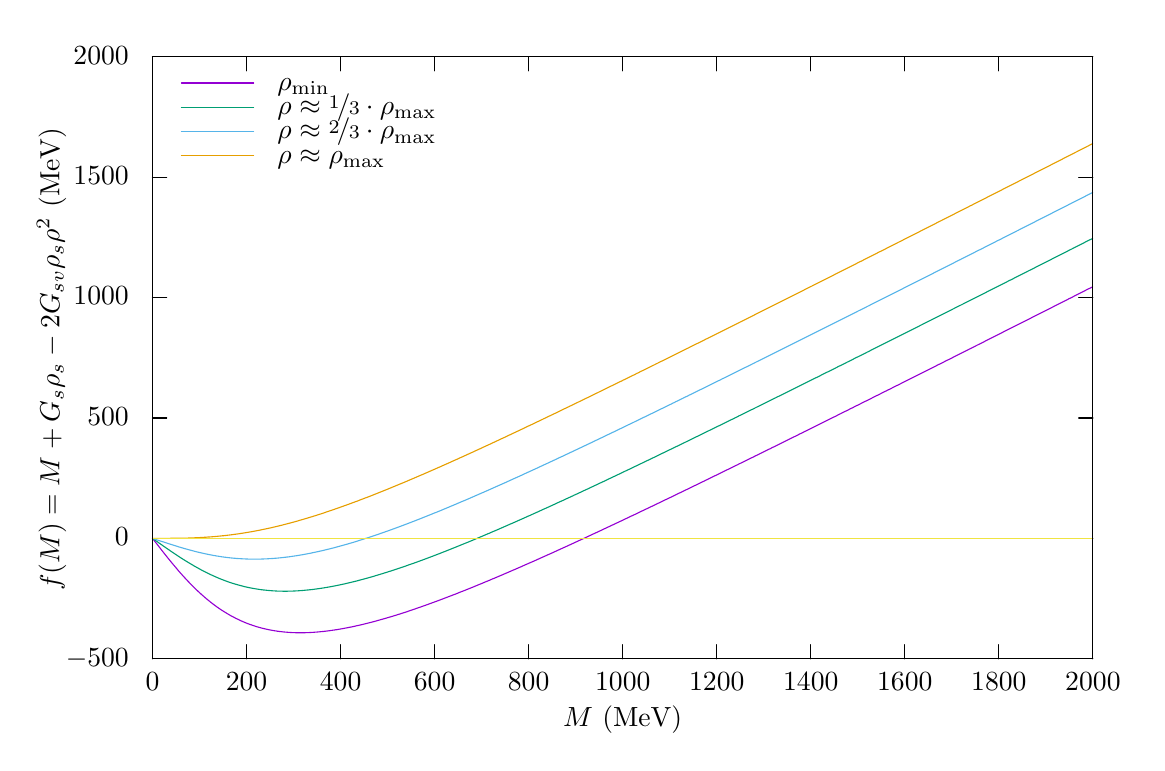
\begin{tikzpicture}[gnuplot]
%% generated with GNUPLOT 5.0p2 (Lua 5.2; terminal rev. 99, script rev. 100)
%% Fri Mar  4 16:19:10 2016
\path (0.000,0.000) rectangle (14.000,9.000);
\gpcolor{color=gp lt color border}
\gpsetlinetype{gp lt border}
\gpsetdashtype{gp dt solid}
\gpsetlinewidth{1.00}
\draw[gp path] (1.504,0.985)--(1.684,0.985);
\draw[gp path] (13.447,0.985)--(13.267,0.985);
\node[gp node right] at (1.320,0.985) {$-500$};
\draw[gp path] (1.504,2.514)--(1.684,2.514);
\draw[gp path] (13.447,2.514)--(13.267,2.514);
\node[gp node right] at (1.320,2.514) {$0$};
\draw[gp path] (1.504,4.043)--(1.684,4.043);
\draw[gp path] (13.447,4.043)--(13.267,4.043);
\node[gp node right] at (1.320,4.043) {$500$};
\draw[gp path] (1.504,5.573)--(1.684,5.573);
\draw[gp path] (13.447,5.573)--(13.267,5.573);
\node[gp node right] at (1.320,5.573) {$1000$};
\draw[gp path] (1.504,7.102)--(1.684,7.102);
\draw[gp path] (13.447,7.102)--(13.267,7.102);
\node[gp node right] at (1.320,7.102) {$1500$};
\draw[gp path] (1.504,8.631)--(1.684,8.631);
\draw[gp path] (13.447,8.631)--(13.267,8.631);
\node[gp node right] at (1.320,8.631) {$2000$};
\draw[gp path] (1.504,0.985)--(1.504,1.165);
\draw[gp path] (1.504,8.631)--(1.504,8.451);
\node[gp node center] at (1.504,0.677) {$0$};
\draw[gp path] (2.698,0.985)--(2.698,1.165);
\draw[gp path] (2.698,8.631)--(2.698,8.451);
\node[gp node center] at (2.698,0.677) {$200$};
\draw[gp path] (3.893,0.985)--(3.893,1.165);
\draw[gp path] (3.893,8.631)--(3.893,8.451);
\node[gp node center] at (3.893,0.677) {$400$};
\draw[gp path] (5.087,0.985)--(5.087,1.165);
\draw[gp path] (5.087,8.631)--(5.087,8.451);
\node[gp node center] at (5.087,0.677) {$600$};
\draw[gp path] (6.281,0.985)--(6.281,1.165);
\draw[gp path] (6.281,8.631)--(6.281,8.451);
\node[gp node center] at (6.281,0.677) {$800$};
\draw[gp path] (7.476,0.985)--(7.476,1.165);
\draw[gp path] (7.476,8.631)--(7.476,8.451);
\node[gp node center] at (7.476,0.677) {$1000$};
\draw[gp path] (8.670,0.985)--(8.670,1.165);
\draw[gp path] (8.670,8.631)--(8.670,8.451);
\node[gp node center] at (8.670,0.677) {$1200$};
\draw[gp path] (9.864,0.985)--(9.864,1.165);
\draw[gp path] (9.864,8.631)--(9.864,8.451);
\node[gp node center] at (9.864,0.677) {$1400$};
\draw[gp path] (11.058,0.985)--(11.058,1.165);
\draw[gp path] (11.058,8.631)--(11.058,8.451);
\node[gp node center] at (11.058,0.677) {$1600$};
\draw[gp path] (12.253,0.985)--(12.253,1.165);
\draw[gp path] (12.253,8.631)--(12.253,8.451);
\node[gp node center] at (12.253,0.677) {$1800$};
\draw[gp path] (13.447,0.985)--(13.447,1.165);
\draw[gp path] (13.447,8.631)--(13.447,8.451);
\node[gp node center] at (13.447,0.677) {$2000$};
\draw[gp path] (1.504,8.631)--(1.504,0.985)--(13.447,0.985)--(13.447,8.631)--cycle;
\node[gp node center,rotate=-270] at (0.246,4.808) {$f(M) = M + G_s\rho_s - 2G_{sv}\rho_s\rho^2$ (MeV)};
\node[gp node center] at (7.475,0.215) {$M$ (MeV)};
\node[gp node left] at (2.972,8.297) {$\rho_{\rm{min}}$};
\gpcolor{rgb color={0.580,0.000,0.827}}
\draw[gp path] (1.872,8.297)--(2.788,8.297);
\draw[gp path] (1.507,2.510)--(1.510,2.506)--(1.513,2.503)--(1.516,2.499)--(1.519,2.495)%
  --(1.522,2.491)--(1.525,2.487)--(1.528,2.483)--(1.531,2.479)--(1.534,2.476)--(1.537,2.472)%
  --(1.540,2.468)--(1.543,2.464)--(1.546,2.460)--(1.549,2.456)--(1.552,2.452)--(1.555,2.449)%
  --(1.558,2.445)--(1.561,2.441)--(1.564,2.437)--(1.567,2.433)--(1.570,2.429)--(1.573,2.425)%
  --(1.576,2.422)--(1.579,2.418)--(1.582,2.414)--(1.585,2.410)--(1.588,2.406)--(1.591,2.402)%
  --(1.594,2.399)--(1.597,2.395)--(1.600,2.391)--(1.603,2.387)--(1.606,2.383)--(1.609,2.380)%
  --(1.611,2.376)--(1.614,2.372)--(1.617,2.368)--(1.620,2.364)--(1.623,2.360)--(1.626,2.357)%
  --(1.629,2.353)--(1.632,2.349)--(1.635,2.345)--(1.638,2.341)--(1.641,2.338)--(1.644,2.334)%
  --(1.647,2.330)--(1.650,2.326)--(1.653,2.323)--(1.656,2.319)--(1.659,2.315)--(1.662,2.311)%
  --(1.665,2.308)--(1.668,2.304)--(1.671,2.300)--(1.674,2.296)--(1.677,2.293)--(1.680,2.289)%
  --(1.683,2.285)--(1.686,2.281)--(1.689,2.278)--(1.692,2.274)--(1.695,2.270)--(1.698,2.266)%
  --(1.701,2.263)--(1.704,2.259)--(1.707,2.255)--(1.710,2.252)--(1.713,2.248)--(1.716,2.244)%
  --(1.719,2.241)--(1.722,2.237)--(1.725,2.233)--(1.728,2.230)--(1.731,2.226)--(1.734,2.222)%
  --(1.737,2.219)--(1.740,2.215)--(1.743,2.211)--(1.746,2.208)--(1.749,2.204)--(1.752,2.200)%
  --(1.755,2.197)--(1.758,2.193)--(1.761,2.190)--(1.764,2.186)--(1.767,2.182)--(1.770,2.179)%
  --(1.773,2.175)--(1.776,2.172)--(1.779,2.168)--(1.782,2.165)--(1.785,2.161)--(1.788,2.157)%
  --(1.791,2.154)--(1.794,2.150)--(1.797,2.147)--(1.800,2.143)--(1.803,2.140)--(1.806,2.136)%
  --(1.809,2.133)--(1.812,2.129)--(1.815,2.126)--(1.818,2.122)--(1.820,2.119)--(1.823,2.115)%
  --(1.826,2.112)--(1.829,2.108)--(1.832,2.105)--(1.835,2.101)--(1.838,2.098)--(1.841,2.095)%
  --(1.844,2.091)--(1.847,2.088)--(1.850,2.084)--(1.853,2.081)--(1.856,2.077)--(1.859,2.074)%
  --(1.862,2.071)--(1.865,2.067)--(1.868,2.064)--(1.871,2.061)--(1.874,2.057)--(1.877,2.054)%
  --(1.880,2.050)--(1.883,2.047)--(1.886,2.044)--(1.889,2.041)--(1.892,2.037)--(1.895,2.034)%
  --(1.898,2.031)--(1.901,2.027)--(1.904,2.024)--(1.907,2.021)--(1.910,2.017)--(1.913,2.014)%
  --(1.916,2.011)--(1.919,2.008)--(1.922,2.004)--(1.925,2.001)--(1.928,1.998)--(1.931,1.995)%
  --(1.934,1.992)--(1.937,1.988)--(1.940,1.985)--(1.943,1.982)--(1.946,1.979)--(1.949,1.976)%
  --(1.952,1.972)--(1.955,1.969)--(1.958,1.966)--(1.961,1.963)--(1.964,1.960)--(1.967,1.957)%
  --(1.970,1.954)--(1.973,1.950)--(1.976,1.947)--(1.979,1.944)--(1.982,1.941)--(1.985,1.938)%
  --(1.988,1.935)--(1.991,1.932)--(1.994,1.929)--(1.997,1.926)--(2.000,1.923)--(2.003,1.920)%
  --(2.006,1.917)--(2.009,1.914)--(2.012,1.911)--(2.015,1.908)--(2.018,1.905)--(2.021,1.902)%
  --(2.024,1.899)--(2.027,1.896)--(2.029,1.893)--(2.032,1.890)--(2.035,1.887)--(2.038,1.884)%
  --(2.041,1.881)--(2.044,1.878)--(2.047,1.875)--(2.050,1.873)--(2.053,1.870)--(2.056,1.867)%
  --(2.059,1.864)--(2.062,1.861)--(2.065,1.858)--(2.068,1.855)--(2.071,1.852)--(2.074,1.850)%
  --(2.077,1.847)--(2.080,1.844)--(2.083,1.841)--(2.086,1.838)--(2.089,1.836)--(2.092,1.833)%
  --(2.095,1.830)--(2.098,1.827)--(2.101,1.825)--(2.104,1.822)--(2.107,1.819)--(2.110,1.816)%
  --(2.113,1.814)--(2.116,1.811)--(2.119,1.808)--(2.122,1.805)--(2.125,1.803)--(2.128,1.800)%
  --(2.131,1.797)--(2.134,1.795)--(2.137,1.792)--(2.140,1.789)--(2.143,1.787)--(2.146,1.784)%
  --(2.149,1.782)--(2.152,1.779)--(2.155,1.776)--(2.158,1.774)--(2.161,1.771)--(2.164,1.769)%
  --(2.167,1.766)--(2.170,1.764)--(2.173,1.761)--(2.176,1.758)--(2.179,1.756)--(2.182,1.753)%
  --(2.185,1.751)--(2.188,1.748)--(2.191,1.746)--(2.194,1.743)--(2.197,1.741)--(2.200,1.738)%
  --(2.203,1.736)--(2.206,1.733)--(2.209,1.731)--(2.212,1.729)--(2.215,1.726)--(2.218,1.724)%
  --(2.221,1.721)--(2.224,1.719)--(2.227,1.716)--(2.230,1.714)--(2.233,1.712)--(2.236,1.709)%
  --(2.238,1.707)--(2.241,1.705)--(2.244,1.702)--(2.247,1.700)--(2.250,1.698)--(2.253,1.695)%
  --(2.256,1.693)--(2.259,1.691)--(2.262,1.688)--(2.265,1.686)--(2.268,1.684)--(2.271,1.682)%
  --(2.274,1.679)--(2.277,1.677)--(2.280,1.675)--(2.283,1.673)--(2.286,1.670)--(2.289,1.668)%
  --(2.292,1.666)--(2.295,1.664)--(2.298,1.661)--(2.301,1.659)--(2.304,1.657)--(2.307,1.655)%
  --(2.310,1.653)--(2.313,1.651)--(2.316,1.648)--(2.319,1.646)--(2.322,1.644)--(2.325,1.642)%
  --(2.328,1.640)--(2.331,1.638)--(2.334,1.636)--(2.337,1.634)--(2.340,1.632)--(2.343,1.629)%
  --(2.346,1.627)--(2.349,1.625)--(2.352,1.623)--(2.355,1.621)--(2.358,1.619)--(2.361,1.617)%
  --(2.364,1.615)--(2.367,1.613)--(2.370,1.611)--(2.373,1.609)--(2.376,1.607)--(2.379,1.605)%
  --(2.382,1.603)--(2.385,1.601)--(2.388,1.599)--(2.391,1.597)--(2.394,1.595)--(2.397,1.594)%
  --(2.400,1.592)--(2.403,1.590)--(2.406,1.588)--(2.409,1.586)--(2.412,1.584)--(2.415,1.582)%
  --(2.418,1.580)--(2.421,1.578)--(2.424,1.577)--(2.427,1.575)--(2.430,1.573)--(2.433,1.571)%
  --(2.436,1.569)--(2.439,1.567)--(2.442,1.566)--(2.445,1.564)--(2.447,1.562)--(2.450,1.560)%
  --(2.453,1.558)--(2.456,1.557)--(2.459,1.555)--(2.462,1.553)--(2.465,1.551)--(2.468,1.550)%
  --(2.471,1.548)--(2.474,1.546)--(2.477,1.544)--(2.480,1.543)--(2.483,1.541)--(2.486,1.539)%
  --(2.489,1.538)--(2.492,1.536)--(2.495,1.534)--(2.498,1.533)--(2.501,1.531)--(2.504,1.529)%
  --(2.507,1.528)--(2.510,1.526)--(2.513,1.524)--(2.516,1.523)--(2.519,1.521)--(2.522,1.520)%
  --(2.525,1.518)--(2.528,1.516)--(2.531,1.515)--(2.534,1.513)--(2.537,1.512)--(2.540,1.510)%
  --(2.543,1.509)--(2.546,1.507)--(2.549,1.506)--(2.552,1.504)--(2.555,1.502)--(2.558,1.501)%
  --(2.561,1.499)--(2.564,1.498)--(2.567,1.496)--(2.570,1.495)--(2.573,1.493)--(2.576,1.492)%
  --(2.579,1.491)--(2.582,1.489)--(2.585,1.488)--(2.588,1.486)--(2.591,1.485)--(2.594,1.483)%
  --(2.597,1.482)--(2.600,1.481)--(2.603,1.479)--(2.606,1.478)--(2.609,1.476)--(2.612,1.475)%
  --(2.615,1.474)--(2.618,1.472)--(2.621,1.471)--(2.624,1.469)--(2.627,1.468)--(2.630,1.467)%
  --(2.633,1.465)--(2.636,1.464)--(2.639,1.463)--(2.642,1.462)--(2.645,1.460)--(2.648,1.459)%
  --(2.651,1.458)--(2.654,1.456)--(2.656,1.455)--(2.659,1.454)--(2.662,1.453)--(2.665,1.451)%
  --(2.668,1.450)--(2.671,1.449)--(2.674,1.448)--(2.677,1.446)--(2.680,1.445)--(2.683,1.444)%
  --(2.686,1.443)--(2.689,1.441)--(2.692,1.440)--(2.695,1.439)--(2.698,1.438)--(2.701,1.437)%
  --(2.704,1.436)--(2.707,1.434)--(2.710,1.433)--(2.713,1.432)--(2.716,1.431)--(2.719,1.430)%
  --(2.722,1.429)--(2.725,1.428)--(2.728,1.426)--(2.731,1.425)--(2.734,1.424)--(2.737,1.423)%
  --(2.740,1.422)--(2.743,1.421)--(2.746,1.420)--(2.749,1.419)--(2.752,1.418)--(2.755,1.417)%
  --(2.758,1.416)--(2.761,1.415)--(2.764,1.414)--(2.767,1.412)--(2.770,1.411)--(2.773,1.410)%
  --(2.776,1.409)--(2.779,1.408)--(2.782,1.407)--(2.785,1.406)--(2.788,1.405)--(2.791,1.404)%
  --(2.794,1.403)--(2.797,1.402)--(2.800,1.402)--(2.803,1.401)--(2.806,1.400)--(2.809,1.399)%
  --(2.812,1.398)--(2.815,1.397)--(2.818,1.396)--(2.821,1.395)--(2.824,1.394)--(2.827,1.393)%
  --(2.830,1.392)--(2.833,1.391)--(2.836,1.390)--(2.839,1.390)--(2.842,1.389)--(2.845,1.388)%
  --(2.848,1.387)--(2.851,1.386)--(2.854,1.385)--(2.857,1.384)--(2.860,1.384)--(2.863,1.383)%
  --(2.866,1.382)--(2.868,1.381)--(2.871,1.380)--(2.874,1.379)--(2.877,1.379)--(2.880,1.378)%
  --(2.883,1.377)--(2.886,1.376)--(2.889,1.375)--(2.892,1.375)--(2.895,1.374)--(2.898,1.373)%
  --(2.901,1.372)--(2.904,1.372)--(2.907,1.371)--(2.910,1.370)--(2.913,1.369)--(2.916,1.369)%
  --(2.919,1.368)--(2.922,1.367)--(2.925,1.366)--(2.928,1.366)--(2.931,1.365)--(2.934,1.364)%
  --(2.937,1.364)--(2.940,1.363)--(2.943,1.362)--(2.946,1.362)--(2.949,1.361)--(2.952,1.360)%
  --(2.955,1.360)--(2.958,1.359)--(2.961,1.358)--(2.964,1.358)--(2.967,1.357)--(2.970,1.356)%
  --(2.973,1.356)--(2.976,1.355)--(2.979,1.355)--(2.982,1.354)--(2.985,1.353)--(2.988,1.353)%
  --(2.991,1.352)--(2.994,1.352)--(2.997,1.351)--(3.000,1.350)--(3.003,1.350)--(3.006,1.349)%
  --(3.009,1.349)--(3.012,1.348)--(3.015,1.348)--(3.018,1.347)--(3.021,1.347)--(3.024,1.346)%
  --(3.027,1.345)--(3.030,1.345)--(3.033,1.344)--(3.036,1.344)--(3.039,1.343)--(3.042,1.343)%
  --(3.045,1.342)--(3.048,1.342)--(3.051,1.341)--(3.054,1.341)--(3.057,1.340)--(3.060,1.340)%
  --(3.063,1.339)--(3.066,1.339)--(3.069,1.339)--(3.072,1.338)--(3.075,1.338)--(3.077,1.337)%
  --(3.080,1.337)--(3.083,1.336)--(3.086,1.336)--(3.089,1.335)--(3.092,1.335)--(3.095,1.335)%
  --(3.098,1.334)--(3.101,1.334)--(3.104,1.333)--(3.107,1.333)--(3.110,1.333)--(3.113,1.332)%
  --(3.116,1.332)--(3.119,1.331)--(3.122,1.331)--(3.125,1.331)--(3.128,1.330)--(3.131,1.330)%
  --(3.134,1.330)--(3.137,1.329)--(3.140,1.329)--(3.143,1.329)--(3.146,1.328)--(3.149,1.328)%
  --(3.152,1.328)--(3.155,1.327)--(3.158,1.327)--(3.161,1.327)--(3.164,1.326)--(3.167,1.326)%
  --(3.170,1.326)--(3.173,1.325)--(3.176,1.325)--(3.179,1.325)--(3.182,1.325)--(3.185,1.324)%
  --(3.188,1.324)--(3.191,1.324)--(3.194,1.324)--(3.197,1.323)--(3.200,1.323)--(3.203,1.323)%
  --(3.206,1.323)--(3.209,1.322)--(3.212,1.322)--(3.215,1.322)--(3.218,1.322)--(3.221,1.321)%
  --(3.224,1.321)--(3.227,1.321)--(3.230,1.321)--(3.233,1.321)--(3.236,1.320)--(3.239,1.320)%
  --(3.242,1.320)--(3.245,1.320)--(3.248,1.320)--(3.251,1.319)--(3.254,1.319)--(3.257,1.319)%
  --(3.260,1.319)--(3.263,1.319)--(3.266,1.319)--(3.269,1.318)--(3.272,1.318)--(3.275,1.318)%
  --(3.278,1.318)--(3.281,1.318)--(3.284,1.318)--(3.286,1.318)--(3.289,1.317)--(3.292,1.317)%
  --(3.295,1.317)--(3.298,1.317)--(3.301,1.317)--(3.304,1.317)--(3.307,1.317)--(3.310,1.317)%
  --(3.313,1.317)--(3.316,1.317)--(3.319,1.316)--(3.322,1.316)--(3.325,1.316)--(3.328,1.316)%
  --(3.331,1.316)--(3.334,1.316)--(3.337,1.316)--(3.340,1.316)--(3.343,1.316)--(3.346,1.316)%
  --(3.349,1.316)--(3.352,1.316)--(3.355,1.316)--(3.358,1.316)--(3.361,1.316)--(3.364,1.316)%
  --(3.367,1.316)--(3.370,1.316)--(3.373,1.316)--(3.376,1.316)--(3.379,1.316)--(3.382,1.316)%
  --(3.385,1.316)--(3.388,1.316)--(3.391,1.316)--(3.394,1.316)--(3.397,1.316)--(3.400,1.316)%
  --(3.403,1.316)--(3.406,1.316)--(3.409,1.316)--(3.412,1.316)--(3.415,1.316)--(3.418,1.316)%
  --(3.421,1.316)--(3.424,1.316)--(3.427,1.316)--(3.430,1.316)--(3.433,1.316)--(3.436,1.316)%
  --(3.439,1.316)--(3.442,1.316)--(3.445,1.316)--(3.448,1.317)--(3.451,1.317)--(3.454,1.317)%
  --(3.457,1.317)--(3.460,1.317)--(3.463,1.317)--(3.466,1.317)--(3.469,1.317)--(3.472,1.317)%
  --(3.475,1.317)--(3.478,1.318)--(3.481,1.318)--(3.484,1.318)--(3.487,1.318)--(3.490,1.318)%
  --(3.493,1.318)--(3.495,1.318)--(3.498,1.318)--(3.501,1.319)--(3.504,1.319)--(3.507,1.319)%
  --(3.510,1.319)--(3.513,1.319)--(3.516,1.319)--(3.519,1.319)--(3.522,1.320)--(3.525,1.320)%
  --(3.528,1.320)--(3.531,1.320)--(3.534,1.320)--(3.537,1.321)--(3.540,1.321)--(3.543,1.321)%
  --(3.546,1.321)--(3.549,1.321)--(3.552,1.321)--(3.555,1.322)--(3.558,1.322)--(3.561,1.322)%
  --(3.564,1.322)--(3.567,1.323)--(3.570,1.323)--(3.573,1.323)--(3.576,1.323)--(3.579,1.323)%
  --(3.582,1.324)--(3.585,1.324)--(3.588,1.324)--(3.591,1.324)--(3.594,1.325)--(3.597,1.325)%
  --(3.600,1.325)--(3.603,1.325)--(3.606,1.326)--(3.609,1.326)--(3.612,1.326)--(3.615,1.326)%
  --(3.618,1.327)--(3.621,1.327)--(3.624,1.327)--(3.627,1.327)--(3.630,1.328)--(3.633,1.328)%
  --(3.636,1.328)--(3.639,1.329)--(3.642,1.329)--(3.645,1.329)--(3.648,1.330)--(3.651,1.330)%
  --(3.654,1.330)--(3.657,1.330)--(3.660,1.331)--(3.663,1.331)--(3.666,1.331)--(3.669,1.332)%
  --(3.672,1.332)--(3.675,1.332)--(3.678,1.333)--(3.681,1.333)--(3.684,1.333)--(3.687,1.334)%
  --(3.690,1.334)--(3.693,1.334)--(3.696,1.335)--(3.699,1.335)--(3.702,1.335)--(3.704,1.336)%
  --(3.707,1.336)--(3.710,1.336)--(3.713,1.337)--(3.716,1.337)--(3.719,1.338)--(3.722,1.338)%
  --(3.725,1.338)--(3.728,1.339)--(3.731,1.339)--(3.734,1.339)--(3.737,1.340)--(3.740,1.340)%
  --(3.743,1.341)--(3.746,1.341)--(3.749,1.341)--(3.752,1.342)--(3.755,1.342)--(3.758,1.343)%
  --(3.761,1.343)--(3.764,1.343)--(3.767,1.344)--(3.770,1.344)--(3.773,1.345)--(3.776,1.345)%
  --(3.779,1.345)--(3.782,1.346)--(3.785,1.346)--(3.788,1.347)--(3.791,1.347)--(3.794,1.348)%
  --(3.797,1.348)--(3.800,1.348)--(3.803,1.349)--(3.806,1.349)--(3.809,1.350)--(3.812,1.350)%
  --(3.815,1.351)--(3.818,1.351)--(3.821,1.352)--(3.824,1.352)--(3.827,1.353)--(3.830,1.353)%
  --(3.833,1.353)--(3.836,1.354)--(3.839,1.354)--(3.842,1.355)--(3.845,1.355)--(3.848,1.356)%
  --(3.851,1.356)--(3.854,1.357)--(3.857,1.357)--(3.860,1.358)--(3.863,1.358)--(3.866,1.359)%
  --(3.869,1.359)--(3.872,1.360)--(3.875,1.360)--(3.878,1.361)--(3.881,1.361)--(3.884,1.362)%
  --(3.887,1.362)--(3.890,1.363)--(3.893,1.363)--(3.896,1.364)--(3.899,1.364)--(3.902,1.365)%
  --(3.905,1.365)--(3.908,1.366)--(3.911,1.366)--(3.914,1.367)--(3.916,1.368)--(3.919,1.368)%
  --(3.922,1.369)--(3.925,1.369)--(3.928,1.370)--(3.931,1.370)--(3.934,1.371)--(3.937,1.371)%
  --(3.940,1.372)--(3.943,1.372)--(3.946,1.373)--(3.949,1.374)--(3.952,1.374)--(3.955,1.375)%
  --(3.958,1.375)--(3.961,1.376)--(3.964,1.376)--(3.967,1.377)--(3.970,1.378)--(3.973,1.378)%
  --(3.976,1.379)--(3.979,1.379)--(3.982,1.380)--(3.985,1.380)--(3.988,1.381)--(3.991,1.382)%
  --(3.994,1.382)--(3.997,1.383)--(4.000,1.383)--(4.003,1.384)--(4.006,1.385)--(4.009,1.385)%
  --(4.012,1.386)--(4.015,1.386)--(4.018,1.387)--(4.021,1.388)--(4.024,1.388)--(4.027,1.389)%
  --(4.030,1.389)--(4.033,1.390)--(4.036,1.391)--(4.039,1.391)--(4.042,1.392)--(4.045,1.393)%
  --(4.048,1.393)--(4.051,1.394)--(4.054,1.395)--(4.057,1.395)--(4.060,1.396)--(4.063,1.396)%
  --(4.066,1.397)--(4.069,1.398)--(4.072,1.398)--(4.075,1.399)--(4.078,1.400)--(4.081,1.400)%
  --(4.084,1.401)--(4.087,1.402)--(4.090,1.402)--(4.093,1.403)--(4.096,1.404)--(4.099,1.404)%
  --(4.102,1.405)--(4.105,1.406)--(4.108,1.406)--(4.111,1.407)--(4.114,1.408)--(4.117,1.408)%
  --(4.120,1.409)--(4.123,1.410)--(4.125,1.410)--(4.128,1.411)--(4.131,1.412)--(4.134,1.412)%
  --(4.137,1.413)--(4.140,1.414)--(4.143,1.414)--(4.146,1.415)--(4.149,1.416)--(4.152,1.417)%
  --(4.155,1.417)--(4.158,1.418)--(4.161,1.419)--(4.164,1.419)--(4.167,1.420)--(4.170,1.421)%
  --(4.173,1.422)--(4.176,1.422)--(4.179,1.423)--(4.182,1.424)--(4.185,1.424)--(4.188,1.425)%
  --(4.191,1.426)--(4.194,1.427)--(4.197,1.427)--(4.200,1.428)--(4.203,1.429)--(4.206,1.429)%
  --(4.209,1.430)--(4.212,1.431)--(4.215,1.432)--(4.218,1.432)--(4.221,1.433)--(4.224,1.434)%
  --(4.227,1.435)--(4.230,1.435)--(4.233,1.436)--(4.236,1.437)--(4.239,1.438)--(4.242,1.438)%
  --(4.245,1.439)--(4.248,1.440)--(4.251,1.441)--(4.254,1.441)--(4.257,1.442)--(4.260,1.443)%
  --(4.263,1.444)--(4.266,1.444)--(4.269,1.445)--(4.272,1.446)--(4.275,1.447)--(4.278,1.448)%
  --(4.281,1.448)--(4.284,1.449)--(4.287,1.450)--(4.290,1.451)--(4.293,1.451)--(4.296,1.452)%
  --(4.299,1.453)--(4.302,1.454)--(4.305,1.455)--(4.308,1.455)--(4.311,1.456)--(4.314,1.457)%
  --(4.317,1.458)--(4.320,1.459)--(4.323,1.459)--(4.326,1.460)--(4.329,1.461)--(4.332,1.462)%
  --(4.334,1.463)--(4.337,1.463)--(4.340,1.464)--(4.343,1.465)--(4.346,1.466)--(4.349,1.467)%
  --(4.352,1.467)--(4.355,1.468)--(4.358,1.469)--(4.361,1.470)--(4.364,1.471)--(4.367,1.472)%
  --(4.370,1.472)--(4.373,1.473)--(4.376,1.474)--(4.379,1.475)--(4.382,1.476)--(4.385,1.477)%
  --(4.388,1.477)--(4.391,1.478)--(4.394,1.479)--(4.397,1.480)--(4.400,1.481)--(4.403,1.482)%
  --(4.406,1.482)--(4.409,1.483)--(4.412,1.484)--(4.415,1.485)--(4.418,1.486)--(4.421,1.487)%
  --(4.424,1.487)--(4.427,1.488)--(4.430,1.489)--(4.433,1.490)--(4.436,1.491)--(4.439,1.492)%
  --(4.442,1.493)--(4.445,1.493)--(4.448,1.494)--(4.451,1.495)--(4.454,1.496)--(4.457,1.497)%
  --(4.460,1.498)--(4.463,1.499)--(4.466,1.500)--(4.469,1.500)--(4.472,1.501)--(4.475,1.502)%
  --(4.478,1.503)--(4.481,1.504)--(4.484,1.505)--(4.487,1.506)--(4.490,1.507)--(4.493,1.507)%
  --(4.496,1.508)--(4.499,1.509)--(4.502,1.510)--(4.505,1.511)--(4.508,1.512)--(4.511,1.513)%
  --(4.514,1.514)--(4.517,1.515)--(4.520,1.515)--(4.523,1.516)--(4.526,1.517)--(4.529,1.518)%
  --(4.532,1.519)--(4.535,1.520)--(4.538,1.521)--(4.541,1.522)--(4.543,1.523)--(4.546,1.524)%
  --(4.549,1.524)--(4.552,1.525)--(4.555,1.526)--(4.558,1.527)--(4.561,1.528)--(4.564,1.529)%
  --(4.567,1.530)--(4.570,1.531)--(4.573,1.532)--(4.576,1.533)--(4.579,1.534)--(4.582,1.535)%
  --(4.585,1.535)--(4.588,1.536)--(4.591,1.537)--(4.594,1.538)--(4.597,1.539)--(4.600,1.540)%
  --(4.603,1.541)--(4.606,1.542)--(4.609,1.543)--(4.612,1.544)--(4.615,1.545)--(4.618,1.546)%
  --(4.621,1.547)--(4.624,1.548)--(4.627,1.549)--(4.630,1.550)--(4.633,1.550)--(4.636,1.551)%
  --(4.639,1.552)--(4.642,1.553)--(4.645,1.554)--(4.648,1.555)--(4.651,1.556)--(4.654,1.557)%
  --(4.657,1.558)--(4.660,1.559)--(4.663,1.560)--(4.666,1.561)--(4.669,1.562)--(4.672,1.563)%
  --(4.675,1.564)--(4.678,1.565)--(4.681,1.566)--(4.684,1.567)--(4.687,1.568)--(4.690,1.569)%
  --(4.693,1.570)--(4.696,1.571)--(4.699,1.572)--(4.702,1.573)--(4.705,1.573)--(4.708,1.574)%
  --(4.711,1.575)--(4.714,1.576)--(4.717,1.577)--(4.720,1.578)--(4.723,1.579)--(4.726,1.580)%
  --(4.729,1.581)--(4.732,1.582)--(4.735,1.583)--(4.738,1.584)--(4.741,1.585)--(4.744,1.586)%
  --(4.747,1.587)--(4.750,1.588)--(4.752,1.589)--(4.755,1.590)--(4.758,1.591)--(4.761,1.592)%
  --(4.764,1.593)--(4.767,1.594)--(4.770,1.595)--(4.773,1.596)--(4.776,1.597)--(4.779,1.598)%
  --(4.782,1.599)--(4.785,1.600)--(4.788,1.601)--(4.791,1.602)--(4.794,1.603)--(4.797,1.604)%
  --(4.800,1.605)--(4.803,1.606)--(4.806,1.607)--(4.809,1.608)--(4.812,1.609)--(4.815,1.610)%
  --(4.818,1.611)--(4.821,1.612)--(4.824,1.613)--(4.827,1.614)--(4.830,1.615)--(4.833,1.616)%
  --(4.836,1.617)--(4.839,1.618)--(4.842,1.619)--(4.845,1.620)--(4.848,1.622)--(4.851,1.623)%
  --(4.854,1.624)--(4.857,1.625)--(4.860,1.626)--(4.863,1.627)--(4.866,1.628)--(4.869,1.629)%
  --(4.872,1.630)--(4.875,1.631)--(4.878,1.632)--(4.881,1.633)--(4.884,1.634)--(4.887,1.635)%
  --(4.890,1.636)--(4.893,1.637)--(4.896,1.638)--(4.899,1.639)--(4.902,1.640)--(4.905,1.641)%
  --(4.908,1.642)--(4.911,1.643)--(4.914,1.644)--(4.917,1.645)--(4.920,1.646)--(4.923,1.647)%
  --(4.926,1.649)--(4.929,1.650)--(4.932,1.651)--(4.935,1.652)--(4.938,1.653)--(4.941,1.654)%
  --(4.944,1.655)--(4.947,1.656)--(4.950,1.657)--(4.953,1.658)--(4.956,1.659)--(4.959,1.660)%
  --(4.961,1.661)--(4.964,1.662)--(4.967,1.663)--(4.970,1.664)--(4.973,1.665)--(4.976,1.667)%
  --(4.979,1.668)--(4.982,1.669)--(4.985,1.670)--(4.988,1.671)--(4.991,1.672)--(4.994,1.673)%
  --(4.997,1.674)--(5.000,1.675)--(5.003,1.676)--(5.006,1.677)--(5.009,1.678)--(5.012,1.679)%
  --(5.015,1.681)--(5.018,1.682)--(5.021,1.683)--(5.024,1.684)--(5.027,1.685)--(5.030,1.686)%
  --(5.033,1.687)--(5.036,1.688)--(5.039,1.689)--(5.042,1.690)--(5.045,1.691)--(5.048,1.692)%
  --(5.051,1.694)--(5.054,1.695)--(5.057,1.696)--(5.060,1.697)--(5.063,1.698)--(5.066,1.699)%
  --(5.069,1.700)--(5.072,1.701)--(5.075,1.702)--(5.078,1.703)--(5.081,1.704)--(5.084,1.706)%
  --(5.087,1.707)--(5.090,1.708)--(5.093,1.709)--(5.096,1.710)--(5.099,1.711)--(5.102,1.712)%
  --(5.105,1.713)--(5.108,1.714)--(5.111,1.715)--(5.114,1.717)--(5.117,1.718)--(5.120,1.719)%
  --(5.123,1.720)--(5.126,1.721)--(5.129,1.722)--(5.132,1.723)--(5.135,1.724)--(5.138,1.725)%
  --(5.141,1.727)--(5.144,1.728)--(5.147,1.729)--(5.150,1.730)--(5.153,1.731)--(5.156,1.732)%
  --(5.159,1.733)--(5.162,1.734)--(5.165,1.736)--(5.168,1.737)--(5.171,1.738)--(5.173,1.739)%
  --(5.176,1.740)--(5.179,1.741)--(5.182,1.742)--(5.185,1.743)--(5.188,1.745)--(5.191,1.746)%
  --(5.194,1.747)--(5.197,1.748)--(5.200,1.749)--(5.203,1.750)--(5.206,1.751)--(5.209,1.752)%
  --(5.212,1.754)--(5.215,1.755)--(5.218,1.756)--(5.221,1.757)--(5.224,1.758)--(5.227,1.759)%
  --(5.230,1.760)--(5.233,1.762)--(5.236,1.763)--(5.239,1.764)--(5.242,1.765)--(5.245,1.766)%
  --(5.248,1.767)--(5.251,1.768)--(5.254,1.770)--(5.257,1.771)--(5.260,1.772)--(5.263,1.773)%
  --(5.266,1.774)--(5.269,1.775)--(5.272,1.776)--(5.275,1.778)--(5.278,1.779)--(5.281,1.780)%
  --(5.284,1.781)--(5.287,1.782)--(5.290,1.783)--(5.293,1.784)--(5.296,1.786)--(5.299,1.787)%
  --(5.302,1.788)--(5.305,1.789)--(5.308,1.790)--(5.311,1.791)--(5.314,1.793)--(5.317,1.794)%
  --(5.320,1.795)--(5.323,1.796)--(5.326,1.797)--(5.329,1.798)--(5.332,1.799)--(5.335,1.801)%
  --(5.338,1.802)--(5.341,1.803)--(5.344,1.804)--(5.347,1.805)--(5.350,1.806)--(5.353,1.808)%
  --(5.356,1.809)--(5.359,1.810)--(5.362,1.811)--(5.365,1.812)--(5.368,1.813)--(5.371,1.815)%
  --(5.374,1.816)--(5.377,1.817)--(5.380,1.818)--(5.382,1.819)--(5.385,1.821)--(5.388,1.822)%
  --(5.391,1.823)--(5.394,1.824)--(5.397,1.825)--(5.400,1.826)--(5.403,1.828)--(5.406,1.829)%
  --(5.409,1.830)--(5.412,1.831)--(5.415,1.832)--(5.418,1.833)--(5.421,1.835)--(5.424,1.836)%
  --(5.427,1.837)--(5.430,1.838)--(5.433,1.839)--(5.436,1.841)--(5.439,1.842)--(5.442,1.843)%
  --(5.445,1.844)--(5.448,1.845)--(5.451,1.847)--(5.454,1.848)--(5.457,1.849)--(5.460,1.850)%
  --(5.463,1.851)--(5.466,1.852)--(5.469,1.854)--(5.472,1.855)--(5.475,1.856)--(5.478,1.857)%
  --(5.481,1.858)--(5.484,1.860)--(5.487,1.861)--(5.490,1.862)--(5.493,1.863)--(5.496,1.864)%
  --(5.499,1.866)--(5.502,1.867)--(5.505,1.868)--(5.508,1.869)--(5.511,1.870)--(5.514,1.872)%
  --(5.517,1.873)--(5.520,1.874)--(5.523,1.875)--(5.526,1.876)--(5.529,1.878)--(5.532,1.879)%
  --(5.535,1.880)--(5.538,1.881)--(5.541,1.882)--(5.544,1.884)--(5.547,1.885)--(5.550,1.886)%
  --(5.553,1.887)--(5.556,1.888)--(5.559,1.890)--(5.562,1.891)--(5.565,1.892)--(5.568,1.893)%
  --(5.571,1.895)--(5.574,1.896)--(5.577,1.897)--(5.580,1.898)--(5.583,1.899)--(5.586,1.901)%
  --(5.589,1.902)--(5.591,1.903)--(5.594,1.904)--(5.597,1.905)--(5.600,1.907)--(5.603,1.908)%
  --(5.606,1.909)--(5.609,1.910)--(5.612,1.912)--(5.615,1.913)--(5.618,1.914)--(5.621,1.915)%
  --(5.624,1.916)--(5.627,1.918)--(5.630,1.919)--(5.633,1.920)--(5.636,1.921)--(5.639,1.923)%
  --(5.642,1.924)--(5.645,1.925)--(5.648,1.926)--(5.651,1.927)--(5.654,1.929)--(5.657,1.930)%
  --(5.660,1.931)--(5.663,1.932)--(5.666,1.934)--(5.669,1.935)--(5.672,1.936)--(5.675,1.937)%
  --(5.678,1.939)--(5.681,1.940)--(5.684,1.941)--(5.687,1.942)--(5.690,1.943)--(5.693,1.945)%
  --(5.696,1.946)--(5.699,1.947)--(5.702,1.948)--(5.705,1.950)--(5.708,1.951)--(5.711,1.952)%
  --(5.714,1.953)--(5.717,1.955)--(5.720,1.956)--(5.723,1.957)--(5.726,1.958)--(5.729,1.960)%
  --(5.732,1.961)--(5.735,1.962)--(5.738,1.963)--(5.741,1.965)--(5.744,1.966)--(5.747,1.967)%
  --(5.750,1.968)--(5.753,1.970)--(5.756,1.971)--(5.759,1.972)--(5.762,1.973)--(5.765,1.974)%
  --(5.768,1.976)--(5.771,1.977)--(5.774,1.978)--(5.777,1.979)--(5.780,1.981)--(5.783,1.982)%
  --(5.786,1.983)--(5.789,1.984)--(5.792,1.986)--(5.795,1.987)--(5.798,1.988)--(5.800,1.989)%
  --(5.803,1.991)--(5.806,1.992)--(5.809,1.993)--(5.812,1.995)--(5.815,1.996)--(5.818,1.997)%
  --(5.821,1.998)--(5.824,2.000)--(5.827,2.001)--(5.830,2.002)--(5.833,2.003)--(5.836,2.005)%
  --(5.839,2.006)--(5.842,2.007)--(5.845,2.008)--(5.848,2.010)--(5.851,2.011)--(5.854,2.012)%
  --(5.857,2.013)--(5.860,2.015)--(5.863,2.016)--(5.866,2.017)--(5.869,2.018)--(5.872,2.020)%
  --(5.875,2.021)--(5.878,2.022)--(5.881,2.023)--(5.884,2.025)--(5.887,2.026)--(5.890,2.027)%
  --(5.893,2.029)--(5.896,2.030)--(5.899,2.031)--(5.902,2.032)--(5.905,2.034)--(5.908,2.035)%
  --(5.911,2.036)--(5.914,2.037)--(5.917,2.039)--(5.920,2.040)--(5.923,2.041)--(5.926,2.043)%
  --(5.929,2.044)--(5.932,2.045)--(5.935,2.046)--(5.938,2.048)--(5.941,2.049)--(5.944,2.050)%
  --(5.947,2.051)--(5.950,2.053)--(5.953,2.054)--(5.956,2.055)--(5.959,2.057)--(5.962,2.058)%
  --(5.965,2.059)--(5.968,2.060)--(5.971,2.062)--(5.974,2.063)--(5.977,2.064)--(5.980,2.065)%
  --(5.983,2.067)--(5.986,2.068)--(5.989,2.069)--(5.992,2.071)--(5.995,2.072)--(5.998,2.073)%
  --(6.001,2.074)--(6.004,2.076)--(6.007,2.077)--(6.009,2.078)--(6.012,2.080)--(6.015,2.081)%
  --(6.018,2.082)--(6.021,2.083)--(6.024,2.085)--(6.027,2.086)--(6.030,2.087)--(6.033,2.089)%
  --(6.036,2.090)--(6.039,2.091)--(6.042,2.092)--(6.045,2.094)--(6.048,2.095)--(6.051,2.096)%
  --(6.054,2.098)--(6.057,2.099)--(6.060,2.100)--(6.063,2.101)--(6.066,2.103)--(6.069,2.104)%
  --(6.072,2.105)--(6.075,2.107)--(6.078,2.108)--(6.081,2.109)--(6.084,2.111)--(6.087,2.112)%
  --(6.090,2.113)--(6.093,2.114)--(6.096,2.116)--(6.099,2.117)--(6.102,2.118)--(6.105,2.120)%
  --(6.108,2.121)--(6.111,2.122)--(6.114,2.123)--(6.117,2.125)--(6.120,2.126)--(6.123,2.127)%
  --(6.126,2.129)--(6.129,2.130)--(6.132,2.131)--(6.135,2.133)--(6.138,2.134)--(6.141,2.135)%
  --(6.144,2.136)--(6.147,2.138)--(6.150,2.139)--(6.153,2.140)--(6.156,2.142)--(6.159,2.143)%
  --(6.162,2.144)--(6.165,2.146)--(6.168,2.147)--(6.171,2.148)--(6.174,2.150)--(6.177,2.151)%
  --(6.180,2.152)--(6.183,2.153)--(6.186,2.155)--(6.189,2.156)--(6.192,2.157)--(6.195,2.159)%
  --(6.198,2.160)--(6.201,2.161)--(6.204,2.163)--(6.207,2.164)--(6.210,2.165)--(6.213,2.167)%
  --(6.216,2.168)--(6.218,2.169)--(6.221,2.170)--(6.224,2.172)--(6.227,2.173)--(6.230,2.174)%
  --(6.233,2.176)--(6.236,2.177)--(6.239,2.178)--(6.242,2.180)--(6.245,2.181)--(6.248,2.182)%
  --(6.251,2.184)--(6.254,2.185)--(6.257,2.186)--(6.260,2.188)--(6.263,2.189)--(6.266,2.190)%
  --(6.269,2.191)--(6.272,2.193)--(6.275,2.194)--(6.278,2.195)--(6.281,2.197)--(6.284,2.198)%
  --(6.287,2.199)--(6.290,2.201)--(6.293,2.202)--(6.296,2.203)--(6.299,2.205)--(6.302,2.206)%
  --(6.305,2.207)--(6.308,2.209)--(6.311,2.210)--(6.314,2.211)--(6.317,2.213)--(6.320,2.214)%
  --(6.323,2.215)--(6.326,2.217)--(6.329,2.218)--(6.332,2.219)--(6.335,2.221)--(6.338,2.222)%
  --(6.341,2.223)--(6.344,2.224)--(6.347,2.226)--(6.350,2.227)--(6.353,2.228)--(6.356,2.230)%
  --(6.359,2.231)--(6.362,2.232)--(6.365,2.234)--(6.368,2.235)--(6.371,2.236)--(6.374,2.238)%
  --(6.377,2.239)--(6.380,2.240)--(6.383,2.242)--(6.386,2.243)--(6.389,2.244)--(6.392,2.246)%
  --(6.395,2.247)--(6.398,2.248)--(6.401,2.250)--(6.404,2.251)--(6.407,2.252)--(6.410,2.254)%
  --(6.413,2.255)--(6.416,2.256)--(6.419,2.258)--(6.422,2.259)--(6.425,2.260)--(6.428,2.262)%
  --(6.430,2.263)--(6.433,2.264)--(6.436,2.266)--(6.439,2.267)--(6.442,2.268)--(6.445,2.270)%
  --(6.448,2.271)--(6.451,2.272)--(6.454,2.274)--(6.457,2.275)--(6.460,2.276)--(6.463,2.278)%
  --(6.466,2.279)--(6.469,2.280)--(6.472,2.282)--(6.475,2.283)--(6.478,2.284)--(6.481,2.286)%
  --(6.484,2.287)--(6.487,2.288)--(6.490,2.290)--(6.493,2.291)--(6.496,2.292)--(6.499,2.294)%
  --(6.502,2.295)--(6.505,2.297)--(6.508,2.298)--(6.511,2.299)--(6.514,2.301)--(6.517,2.302)%
  --(6.520,2.303)--(6.523,2.305)--(6.526,2.306)--(6.529,2.307)--(6.532,2.309)--(6.535,2.310)%
  --(6.538,2.311)--(6.541,2.313)--(6.544,2.314)--(6.547,2.315)--(6.550,2.317)--(6.553,2.318)%
  --(6.556,2.319)--(6.559,2.321)--(6.562,2.322)--(6.565,2.323)--(6.568,2.325)--(6.571,2.326)%
  --(6.574,2.327)--(6.577,2.329)--(6.580,2.330)--(6.583,2.331)--(6.586,2.333)--(6.589,2.334)%
  --(6.592,2.336)--(6.595,2.337)--(6.598,2.338)--(6.601,2.340)--(6.604,2.341)--(6.607,2.342)%
  --(6.610,2.344)--(6.613,2.345)--(6.616,2.346)--(6.619,2.348)--(6.622,2.349)--(6.625,2.350)%
  --(6.628,2.352)--(6.631,2.353)--(6.634,2.354)--(6.637,2.356)--(6.639,2.357)--(6.642,2.359)%
  --(6.645,2.360)--(6.648,2.361)--(6.651,2.363)--(6.654,2.364)--(6.657,2.365)--(6.660,2.367)%
  --(6.663,2.368)--(6.666,2.369)--(6.669,2.371)--(6.672,2.372)--(6.675,2.373)--(6.678,2.375)%
  --(6.681,2.376)--(6.684,2.378)--(6.687,2.379)--(6.690,2.380)--(6.693,2.382)--(6.696,2.383)%
  --(6.699,2.384)--(6.702,2.386)--(6.705,2.387)--(6.708,2.388)--(6.711,2.390)--(6.714,2.391)%
  --(6.717,2.392)--(6.720,2.394)--(6.723,2.395)--(6.726,2.397)--(6.729,2.398)--(6.732,2.399)%
  --(6.735,2.401)--(6.738,2.402)--(6.741,2.403)--(6.744,2.405)--(6.747,2.406)--(6.750,2.407)%
  --(6.753,2.409)--(6.756,2.410)--(6.759,2.412)--(6.762,2.413)--(6.765,2.414)--(6.768,2.416)%
  --(6.771,2.417)--(6.774,2.418)--(6.777,2.420)--(6.780,2.421)--(6.783,2.422)--(6.786,2.424)%
  --(6.789,2.425)--(6.792,2.427)--(6.795,2.428)--(6.798,2.429)--(6.801,2.431)--(6.804,2.432)%
  --(6.807,2.433)--(6.810,2.435)--(6.813,2.436)--(6.816,2.438)--(6.819,2.439)--(6.822,2.440)%
  --(6.825,2.442)--(6.828,2.443)--(6.831,2.444)--(6.834,2.446)--(6.837,2.447)--(6.840,2.448)%
  --(6.843,2.450)--(6.846,2.451)--(6.848,2.453)--(6.851,2.454)--(6.854,2.455)--(6.857,2.457)%
  --(6.860,2.458)--(6.863,2.459)--(6.866,2.461)--(6.869,2.462)--(6.872,2.464)--(6.875,2.465)%
  --(6.878,2.466)--(6.881,2.468)--(6.884,2.469)--(6.887,2.470)--(6.890,2.472)--(6.893,2.473)%
  --(6.896,2.475)--(6.899,2.476)--(6.902,2.477)--(6.905,2.479)--(6.908,2.480)--(6.911,2.481)%
  --(6.914,2.483)--(6.917,2.484)--(6.920,2.486)--(6.923,2.487)--(6.926,2.488)--(6.929,2.490)%
  --(6.932,2.491)--(6.935,2.492)--(6.938,2.494)--(6.941,2.495)--(6.944,2.497)--(6.947,2.498)%
  --(6.950,2.499)--(6.953,2.501)--(6.956,2.502)--(6.959,2.504)--(6.962,2.505)--(6.965,2.506)%
  --(6.968,2.508)--(6.971,2.509)--(6.974,2.510)--(6.977,2.512)--(6.980,2.513)--(6.983,2.515)%
  --(6.986,2.516)--(6.989,2.517)--(6.992,2.519)--(6.995,2.520)--(6.998,2.521)--(7.001,2.523)%
  --(7.004,2.524)--(7.007,2.526)--(7.010,2.527)--(7.013,2.528)--(7.016,2.530)--(7.019,2.531)%
  --(7.022,2.533)--(7.025,2.534)--(7.028,2.535)--(7.031,2.537)--(7.034,2.538)--(7.037,2.539)%
  --(7.040,2.541)--(7.043,2.542)--(7.046,2.544)--(7.049,2.545)--(7.052,2.546)--(7.055,2.548)%
  --(7.057,2.549)--(7.060,2.551)--(7.063,2.552)--(7.066,2.553)--(7.069,2.555)--(7.072,2.556)%
  --(7.075,2.557)--(7.078,2.559)--(7.081,2.560)--(7.084,2.562)--(7.087,2.563)--(7.090,2.564)%
  --(7.093,2.566)--(7.096,2.567)--(7.099,2.569)--(7.102,2.570)--(7.105,2.571)--(7.108,2.573)%
  --(7.111,2.574)--(7.114,2.576)--(7.117,2.577)--(7.120,2.578)--(7.123,2.580)--(7.126,2.581)%
  --(7.129,2.583)--(7.132,2.584)--(7.135,2.585)--(7.138,2.587)--(7.141,2.588)--(7.144,2.589)%
  --(7.147,2.591)--(7.150,2.592)--(7.153,2.594)--(7.156,2.595)--(7.159,2.596)--(7.162,2.598)%
  --(7.165,2.599)--(7.168,2.601)--(7.171,2.602)--(7.174,2.603)--(7.177,2.605)--(7.180,2.606)%
  --(7.183,2.608)--(7.186,2.609)--(7.189,2.610)--(7.192,2.612)--(7.195,2.613)--(7.198,2.615)%
  --(7.201,2.616)--(7.204,2.617)--(7.207,2.619)--(7.210,2.620)--(7.213,2.622)--(7.216,2.623)%
  --(7.219,2.624)--(7.222,2.626)--(7.225,2.627)--(7.228,2.629)--(7.231,2.630)--(7.234,2.631)%
  --(7.237,2.633)--(7.240,2.634)--(7.243,2.636)--(7.246,2.637)--(7.249,2.638)--(7.252,2.640)%
  --(7.255,2.641)--(7.258,2.643)--(7.261,2.644)--(7.264,2.645)--(7.266,2.647)--(7.269,2.648)%
  --(7.272,2.650)--(7.275,2.651)--(7.278,2.652)--(7.281,2.654)--(7.284,2.655)--(7.287,2.657)%
  --(7.290,2.658)--(7.293,2.659)--(7.296,2.661)--(7.299,2.662)--(7.302,2.664)--(7.305,2.665)%
  --(7.308,2.666)--(7.311,2.668)--(7.314,2.669)--(7.317,2.671)--(7.320,2.672)--(7.323,2.673)%
  --(7.326,2.675)--(7.329,2.676)--(7.332,2.678)--(7.335,2.679)--(7.338,2.680)--(7.341,2.682)%
  --(7.344,2.683)--(7.347,2.685)--(7.350,2.686)--(7.353,2.687)--(7.356,2.689)--(7.359,2.690)%
  --(7.362,2.692)--(7.365,2.693)--(7.368,2.694)--(7.371,2.696)--(7.374,2.697)--(7.377,2.699)%
  --(7.380,2.700)--(7.383,2.702)--(7.386,2.703)--(7.389,2.704)--(7.392,2.706)--(7.395,2.707)%
  --(7.398,2.709)--(7.401,2.710)--(7.404,2.711)--(7.407,2.713)--(7.410,2.714)--(7.413,2.716)%
  --(7.416,2.717)--(7.419,2.718)--(7.422,2.720)--(7.425,2.721)--(7.428,2.723)--(7.431,2.724)%
  --(7.434,2.725)--(7.437,2.727)--(7.440,2.728)--(7.443,2.730)--(7.446,2.731)--(7.449,2.733)%
  --(7.452,2.734)--(7.455,2.735)--(7.458,2.737)--(7.461,2.738)--(7.464,2.740)--(7.467,2.741)%
  --(7.470,2.742)--(7.473,2.744)--(7.476,2.745)--(7.478,2.747)--(7.481,2.748)--(7.484,2.749)%
  --(7.487,2.751)--(7.490,2.752)--(7.493,2.754)--(7.496,2.755)--(7.499,2.757)--(7.502,2.758)%
  --(7.505,2.759)--(7.508,2.761)--(7.511,2.762)--(7.514,2.764)--(7.517,2.765)--(7.520,2.766)%
  --(7.523,2.768)--(7.526,2.769)--(7.529,2.771)--(7.532,2.772)--(7.535,2.773)--(7.538,2.775)%
  --(7.541,2.776)--(7.544,2.778)--(7.547,2.779)--(7.550,2.781)--(7.553,2.782)--(7.556,2.783)%
  --(7.559,2.785)--(7.562,2.786)--(7.565,2.788)--(7.568,2.789)--(7.571,2.790)--(7.574,2.792)%
  --(7.577,2.793)--(7.580,2.795)--(7.583,2.796)--(7.586,2.798)--(7.589,2.799)--(7.592,2.800)%
  --(7.595,2.802)--(7.598,2.803)--(7.601,2.805)--(7.604,2.806)--(7.607,2.807)--(7.610,2.809)%
  --(7.613,2.810)--(7.616,2.812)--(7.619,2.813)--(7.622,2.815)--(7.625,2.816)--(7.628,2.817)%
  --(7.631,2.819)--(7.634,2.820)--(7.637,2.822)--(7.640,2.823)--(7.643,2.825)--(7.646,2.826)%
  --(7.649,2.827)--(7.652,2.829)--(7.655,2.830)--(7.658,2.832)--(7.661,2.833)--(7.664,2.834)%
  --(7.667,2.836)--(7.670,2.837)--(7.673,2.839)--(7.676,2.840)--(7.679,2.842)--(7.682,2.843)%
  --(7.685,2.844)--(7.687,2.846)--(7.690,2.847)--(7.693,2.849)--(7.696,2.850)--(7.699,2.852)%
  --(7.702,2.853)--(7.705,2.854)--(7.708,2.856)--(7.711,2.857)--(7.714,2.859)--(7.717,2.860)%
  --(7.720,2.862)--(7.723,2.863)--(7.726,2.864)--(7.729,2.866)--(7.732,2.867)--(7.735,2.869)%
  --(7.738,2.870)--(7.741,2.871)--(7.744,2.873)--(7.747,2.874)--(7.750,2.876)--(7.753,2.877)%
  --(7.756,2.879)--(7.759,2.880)--(7.762,2.881)--(7.765,2.883)--(7.768,2.884)--(7.771,2.886)%
  --(7.774,2.887)--(7.777,2.889)--(7.780,2.890)--(7.783,2.891)--(7.786,2.893)--(7.789,2.894)%
  --(7.792,2.896)--(7.795,2.897)--(7.798,2.899)--(7.801,2.900)--(7.804,2.901)--(7.807,2.903)%
  --(7.810,2.904)--(7.813,2.906)--(7.816,2.907)--(7.819,2.909)--(7.822,2.910)--(7.825,2.911)%
  --(7.828,2.913)--(7.831,2.914)--(7.834,2.916)--(7.837,2.917)--(7.840,2.919)--(7.843,2.920)%
  --(7.846,2.921)--(7.849,2.923)--(7.852,2.924)--(7.855,2.926)--(7.858,2.927)--(7.861,2.929)%
  --(7.864,2.930)--(7.867,2.931)--(7.870,2.933)--(7.873,2.934)--(7.876,2.936)--(7.879,2.937)%
  --(7.882,2.939)--(7.885,2.940)--(7.888,2.942)--(7.891,2.943)--(7.894,2.944)--(7.896,2.946)%
  --(7.899,2.947)--(7.902,2.949)--(7.905,2.950)--(7.908,2.952)--(7.911,2.953)--(7.914,2.954)%
  --(7.917,2.956)--(7.920,2.957)--(7.923,2.959)--(7.926,2.960)--(7.929,2.962)--(7.932,2.963)%
  --(7.935,2.964)--(7.938,2.966)--(7.941,2.967)--(7.944,2.969)--(7.947,2.970)--(7.950,2.972)%
  --(7.953,2.973)--(7.956,2.974)--(7.959,2.976)--(7.962,2.977)--(7.965,2.979)--(7.968,2.980)%
  --(7.971,2.982)--(7.974,2.983)--(7.977,2.985)--(7.980,2.986)--(7.983,2.987)--(7.986,2.989)%
  --(7.989,2.990)--(7.992,2.992)--(7.995,2.993)--(7.998,2.995)--(8.001,2.996)--(8.004,2.997)%
  --(8.007,2.999)--(8.010,3.000)--(8.013,3.002)--(8.016,3.003)--(8.019,3.005)--(8.022,3.006)%
  --(8.025,3.007)--(8.028,3.009)--(8.031,3.010)--(8.034,3.012)--(8.037,3.013)--(8.040,3.015)%
  --(8.043,3.016)--(8.046,3.018)--(8.049,3.019)--(8.052,3.020)--(8.055,3.022)--(8.058,3.023)%
  --(8.061,3.025)--(8.064,3.026)--(8.067,3.028)--(8.070,3.029)--(8.073,3.031)--(8.076,3.032)%
  --(8.079,3.033)--(8.082,3.035)--(8.085,3.036)--(8.088,3.038)--(8.091,3.039)--(8.094,3.041)%
  --(8.097,3.042)--(8.100,3.043)--(8.103,3.045)--(8.105,3.046)--(8.108,3.048)--(8.111,3.049)%
  --(8.114,3.051)--(8.117,3.052)--(8.120,3.054)--(8.123,3.055)--(8.126,3.056)--(8.129,3.058)%
  --(8.132,3.059)--(8.135,3.061)--(8.138,3.062)--(8.141,3.064)--(8.144,3.065)--(8.147,3.067)%
  --(8.150,3.068)--(8.153,3.069)--(8.156,3.071)--(8.159,3.072)--(8.162,3.074)--(8.165,3.075)%
  --(8.168,3.077)--(8.171,3.078)--(8.174,3.080)--(8.177,3.081)--(8.180,3.082)--(8.183,3.084)%
  --(8.186,3.085)--(8.189,3.087)--(8.192,3.088)--(8.195,3.090)--(8.198,3.091)--(8.201,3.092)%
  --(8.204,3.094)--(8.207,3.095)--(8.210,3.097)--(8.213,3.098)--(8.216,3.100)--(8.219,3.101)%
  --(8.222,3.103)--(8.225,3.104)--(8.228,3.105)--(8.231,3.107)--(8.234,3.108)--(8.237,3.110)%
  --(8.240,3.111)--(8.243,3.113)--(8.246,3.114)--(8.249,3.116)--(8.252,3.117)--(8.255,3.118)%
  --(8.258,3.120)--(8.261,3.121)--(8.264,3.123)--(8.267,3.124)--(8.270,3.126)--(8.273,3.127)%
  --(8.276,3.129)--(8.279,3.130)--(8.282,3.132)--(8.285,3.133)--(8.288,3.134)--(8.291,3.136)%
  --(8.294,3.137)--(8.297,3.139)--(8.300,3.140)--(8.303,3.142)--(8.306,3.143)--(8.309,3.145)%
  --(8.312,3.146)--(8.314,3.147)--(8.317,3.149)--(8.320,3.150)--(8.323,3.152)--(8.326,3.153)%
  --(8.329,3.155)--(8.332,3.156)--(8.335,3.158)--(8.338,3.159)--(8.341,3.160)--(8.344,3.162)%
  --(8.347,3.163)--(8.350,3.165)--(8.353,3.166)--(8.356,3.168)--(8.359,3.169)--(8.362,3.171)%
  --(8.365,3.172)--(8.368,3.174)--(8.371,3.175)--(8.374,3.176)--(8.377,3.178)--(8.380,3.179)%
  --(8.383,3.181)--(8.386,3.182)--(8.389,3.184)--(8.392,3.185)--(8.395,3.187)--(8.398,3.188)%
  --(8.401,3.189)--(8.404,3.191)--(8.407,3.192)--(8.410,3.194)--(8.413,3.195)--(8.416,3.197)%
  --(8.419,3.198)--(8.422,3.200)--(8.425,3.201)--(8.428,3.203)--(8.431,3.204)--(8.434,3.205)%
  --(8.437,3.207)--(8.440,3.208)--(8.443,3.210)--(8.446,3.211)--(8.449,3.213)--(8.452,3.214)%
  --(8.455,3.216)--(8.458,3.217)--(8.461,3.218)--(8.464,3.220)--(8.467,3.221)--(8.470,3.223)%
  --(8.473,3.224)--(8.476,3.226)--(8.479,3.227)--(8.482,3.229)--(8.485,3.230)--(8.488,3.232)%
  --(8.491,3.233)--(8.494,3.234)--(8.497,3.236)--(8.500,3.237)--(8.503,3.239)--(8.506,3.240)%
  --(8.509,3.242)--(8.512,3.243)--(8.515,3.245)--(8.518,3.246)--(8.521,3.248)--(8.523,3.249)%
  --(8.526,3.250)--(8.529,3.252)--(8.532,3.253)--(8.535,3.255)--(8.538,3.256)--(8.541,3.258)%
  --(8.544,3.259)--(8.547,3.261)--(8.550,3.262)--(8.553,3.264)--(8.556,3.265)--(8.559,3.266)%
  --(8.562,3.268)--(8.565,3.269)--(8.568,3.271)--(8.571,3.272)--(8.574,3.274)--(8.577,3.275)%
  --(8.580,3.277)--(8.583,3.278)--(8.586,3.280)--(8.589,3.281)--(8.592,3.282)--(8.595,3.284)%
  --(8.598,3.285)--(8.601,3.287)--(8.604,3.288)--(8.607,3.290)--(8.610,3.291)--(8.613,3.293)%
  --(8.616,3.294)--(8.619,3.296)--(8.622,3.297)--(8.625,3.299)--(8.628,3.300)--(8.631,3.301)%
  --(8.634,3.303)--(8.637,3.304)--(8.640,3.306)--(8.643,3.307)--(8.646,3.309)--(8.649,3.310)%
  --(8.652,3.312)--(8.655,3.313)--(8.658,3.315)--(8.661,3.316)--(8.664,3.317)--(8.667,3.319)%
  --(8.670,3.320)--(8.673,3.322)--(8.676,3.323)--(8.679,3.325)--(8.682,3.326)--(8.685,3.328)%
  --(8.688,3.329)--(8.691,3.331)--(8.694,3.332)--(8.697,3.334)--(8.700,3.335)--(8.703,3.336)%
  --(8.706,3.338)--(8.709,3.339)--(8.712,3.341)--(8.715,3.342)--(8.718,3.344)--(8.721,3.345)%
  --(8.724,3.347)--(8.727,3.348)--(8.730,3.350)--(8.733,3.351)--(8.735,3.352)--(8.738,3.354)%
  --(8.741,3.355)--(8.744,3.357)--(8.747,3.358)--(8.750,3.360)--(8.753,3.361)--(8.756,3.363)%
  --(8.759,3.364)--(8.762,3.366)--(8.765,3.367)--(8.768,3.369)--(8.771,3.370)--(8.774,3.371)%
  --(8.777,3.373)--(8.780,3.374)--(8.783,3.376)--(8.786,3.377)--(8.789,3.379)--(8.792,3.380)%
  --(8.795,3.382)--(8.798,3.383)--(8.801,3.385)--(8.804,3.386)--(8.807,3.388)--(8.810,3.389)%
  --(8.813,3.390)--(8.816,3.392)--(8.819,3.393)--(8.822,3.395)--(8.825,3.396)--(8.828,3.398)%
  --(8.831,3.399)--(8.834,3.401)--(8.837,3.402)--(8.840,3.404)--(8.843,3.405)--(8.846,3.407)%
  --(8.849,3.408)--(8.852,3.409)--(8.855,3.411)--(8.858,3.412)--(8.861,3.414)--(8.864,3.415)%
  --(8.867,3.417)--(8.870,3.418)--(8.873,3.420)--(8.876,3.421)--(8.879,3.423)--(8.882,3.424)%
  --(8.885,3.426)--(8.888,3.427)--(8.891,3.429)--(8.894,3.430)--(8.897,3.431)--(8.900,3.433)%
  --(8.903,3.434)--(8.906,3.436)--(8.909,3.437)--(8.912,3.439)--(8.915,3.440)--(8.918,3.442)%
  --(8.921,3.443)--(8.924,3.445)--(8.927,3.446)--(8.930,3.448)--(8.933,3.449)--(8.936,3.450)%
  --(8.939,3.452)--(8.942,3.453)--(8.944,3.455)--(8.947,3.456)--(8.950,3.458)--(8.953,3.459)%
  --(8.956,3.461)--(8.959,3.462)--(8.962,3.464)--(8.965,3.465)--(8.968,3.467)--(8.971,3.468)%
  --(8.974,3.470)--(8.977,3.471)--(8.980,3.472)--(8.983,3.474)--(8.986,3.475)--(8.989,3.477)%
  --(8.992,3.478)--(8.995,3.480)--(8.998,3.481)--(9.001,3.483)--(9.004,3.484)--(9.007,3.486)%
  --(9.010,3.487)--(9.013,3.489)--(9.016,3.490)--(9.019,3.492)--(9.022,3.493)--(9.025,3.494)%
  --(9.028,3.496)--(9.031,3.497)--(9.034,3.499)--(9.037,3.500)--(9.040,3.502)--(9.043,3.503)%
  --(9.046,3.505)--(9.049,3.506)--(9.052,3.508)--(9.055,3.509)--(9.058,3.511)--(9.061,3.512)%
  --(9.064,3.514)--(9.067,3.515)--(9.070,3.517)--(9.073,3.518)--(9.076,3.519)--(9.079,3.521)%
  --(9.082,3.522)--(9.085,3.524)--(9.088,3.525)--(9.091,3.527)--(9.094,3.528)--(9.097,3.530)%
  --(9.100,3.531)--(9.103,3.533)--(9.106,3.534)--(9.109,3.536)--(9.112,3.537)--(9.115,3.539)%
  --(9.118,3.540)--(9.121,3.541)--(9.124,3.543)--(9.127,3.544)--(9.130,3.546)--(9.133,3.547)%
  --(9.136,3.549)--(9.139,3.550)--(9.142,3.552)--(9.145,3.553)--(9.148,3.555)--(9.151,3.556)%
  --(9.153,3.558)--(9.156,3.559)--(9.159,3.561)--(9.162,3.562)--(9.165,3.564)--(9.168,3.565)%
  --(9.171,3.566)--(9.174,3.568)--(9.177,3.569)--(9.180,3.571)--(9.183,3.572)--(9.186,3.574)%
  --(9.189,3.575)--(9.192,3.577)--(9.195,3.578)--(9.198,3.580)--(9.201,3.581)--(9.204,3.583)%
  --(9.207,3.584)--(9.210,3.586)--(9.213,3.587)--(9.216,3.589)--(9.219,3.590)--(9.222,3.591)%
  --(9.225,3.593)--(9.228,3.594)--(9.231,3.596)--(9.234,3.597)--(9.237,3.599)--(9.240,3.600)%
  --(9.243,3.602)--(9.246,3.603)--(9.249,3.605)--(9.252,3.606)--(9.255,3.608)--(9.258,3.609)%
  --(9.261,3.611)--(9.264,3.612)--(9.267,3.614)--(9.270,3.615)--(9.273,3.617)--(9.276,3.618)%
  --(9.279,3.619)--(9.282,3.621)--(9.285,3.622)--(9.288,3.624)--(9.291,3.625)--(9.294,3.627)%
  --(9.297,3.628)--(9.300,3.630)--(9.303,3.631)--(9.306,3.633)--(9.309,3.634)--(9.312,3.636)%
  --(9.315,3.637)--(9.318,3.639)--(9.321,3.640)--(9.324,3.642)--(9.327,3.643)--(9.330,3.645)%
  --(9.333,3.646)--(9.336,3.647)--(9.339,3.649)--(9.342,3.650)--(9.345,3.652)--(9.348,3.653)%
  --(9.351,3.655)--(9.354,3.656)--(9.357,3.658)--(9.360,3.659)--(9.362,3.661)--(9.365,3.662)%
  --(9.368,3.664)--(9.371,3.665)--(9.374,3.667)--(9.377,3.668)--(9.380,3.670)--(9.383,3.671)%
  --(9.386,3.673)--(9.389,3.674)--(9.392,3.675)--(9.395,3.677)--(9.398,3.678)--(9.401,3.680)%
  --(9.404,3.681)--(9.407,3.683)--(9.410,3.684)--(9.413,3.686)--(9.416,3.687)--(9.419,3.689)%
  --(9.422,3.690)--(9.425,3.692)--(9.428,3.693)--(9.431,3.695)--(9.434,3.696)--(9.437,3.698)%
  --(9.440,3.699)--(9.443,3.701)--(9.446,3.702)--(9.449,3.704)--(9.452,3.705)--(9.455,3.706)%
  --(9.458,3.708)--(9.461,3.709)--(9.464,3.711)--(9.467,3.712)--(9.470,3.714)--(9.473,3.715)%
  --(9.476,3.717)--(9.479,3.718)--(9.482,3.720)--(9.485,3.721)--(9.488,3.723)--(9.491,3.724)%
  --(9.494,3.726)--(9.497,3.727)--(9.500,3.729)--(9.503,3.730)--(9.506,3.732)--(9.509,3.733)%
  --(9.512,3.735)--(9.515,3.736)--(9.518,3.737)--(9.521,3.739)--(9.524,3.740)--(9.527,3.742)%
  --(9.530,3.743)--(9.533,3.745)--(9.536,3.746)--(9.539,3.748)--(9.542,3.749)--(9.545,3.751)%
  --(9.548,3.752)--(9.551,3.754)--(9.554,3.755)--(9.557,3.757)--(9.560,3.758)--(9.563,3.760)%
  --(9.566,3.761)--(9.569,3.763)--(9.571,3.764)--(9.574,3.766)--(9.577,3.767)--(9.580,3.769)%
  --(9.583,3.770)--(9.586,3.771)--(9.589,3.773)--(9.592,3.774)--(9.595,3.776)--(9.598,3.777)%
  --(9.601,3.779)--(9.604,3.780)--(9.607,3.782)--(9.610,3.783)--(9.613,3.785)--(9.616,3.786)%
  --(9.619,3.788)--(9.622,3.789)--(9.625,3.791)--(9.628,3.792)--(9.631,3.794)--(9.634,3.795)%
  --(9.637,3.797)--(9.640,3.798)--(9.643,3.800)--(9.646,3.801)--(9.649,3.803)--(9.652,3.804)%
  --(9.655,3.806)--(9.658,3.807)--(9.661,3.808)--(9.664,3.810)--(9.667,3.811)--(9.670,3.813)%
  --(9.673,3.814)--(9.676,3.816)--(9.679,3.817)--(9.682,3.819)--(9.685,3.820)--(9.688,3.822)%
  --(9.691,3.823)--(9.694,3.825)--(9.697,3.826)--(9.700,3.828)--(9.703,3.829)--(9.706,3.831)%
  --(9.709,3.832)--(9.712,3.834)--(9.715,3.835)--(9.718,3.837)--(9.721,3.838)--(9.724,3.840)%
  --(9.727,3.841)--(9.730,3.843)--(9.733,3.844)--(9.736,3.845)--(9.739,3.847)--(9.742,3.848)%
  --(9.745,3.850)--(9.748,3.851)--(9.751,3.853)--(9.754,3.854)--(9.757,3.856)--(9.760,3.857)%
  --(9.763,3.859)--(9.766,3.860)--(9.769,3.862)--(9.772,3.863)--(9.775,3.865)--(9.778,3.866)%
  --(9.780,3.868)--(9.783,3.869)--(9.786,3.871)--(9.789,3.872)--(9.792,3.874)--(9.795,3.875)%
  --(9.798,3.877)--(9.801,3.878)--(9.804,3.880)--(9.807,3.881)--(9.810,3.883)--(9.813,3.884)%
  --(9.816,3.885)--(9.819,3.887)--(9.822,3.888)--(9.825,3.890)--(9.828,3.891)--(9.831,3.893)%
  --(9.834,3.894)--(9.837,3.896)--(9.840,3.897)--(9.843,3.899)--(9.846,3.900)--(9.849,3.902)%
  --(9.852,3.903)--(9.855,3.905)--(9.858,3.906)--(9.861,3.908)--(9.864,3.909)--(9.867,3.911)%
  --(9.870,3.912)--(9.873,3.914)--(9.876,3.915)--(9.879,3.917)--(9.882,3.918)--(9.885,3.920)%
  --(9.888,3.921)--(9.891,3.923)--(9.894,3.924)--(9.897,3.926)--(9.900,3.927)--(9.903,3.929)%
  --(9.906,3.930)--(9.909,3.931)--(9.912,3.933)--(9.915,3.934)--(9.918,3.936)--(9.921,3.937)%
  --(9.924,3.939)--(9.927,3.940)--(9.930,3.942)--(9.933,3.943)--(9.936,3.945)--(9.939,3.946)%
  --(9.942,3.948)--(9.945,3.949)--(9.948,3.951)--(9.951,3.952)--(9.954,3.954)--(9.957,3.955)%
  --(9.960,3.957)--(9.963,3.958)--(9.966,3.960)--(9.969,3.961)--(9.972,3.963)--(9.975,3.964)%
  --(9.978,3.966)--(9.981,3.967)--(9.984,3.969)--(9.987,3.970)--(9.990,3.972)--(9.992,3.973)%
  --(9.995,3.975)--(9.998,3.976)--(10.001,3.978)--(10.004,3.979)--(10.007,3.980)--(10.010,3.982)%
  --(10.013,3.983)--(10.016,3.985)--(10.019,3.986)--(10.022,3.988)--(10.025,3.989)--(10.028,3.991)%
  --(10.031,3.992)--(10.034,3.994)--(10.037,3.995)--(10.040,3.997)--(10.043,3.998)--(10.046,4.000)%
  --(10.049,4.001)--(10.052,4.003)--(10.055,4.004)--(10.058,4.006)--(10.061,4.007)--(10.064,4.009)%
  --(10.067,4.010)--(10.070,4.012)--(10.073,4.013)--(10.076,4.015)--(10.079,4.016)--(10.082,4.018)%
  --(10.085,4.019)--(10.088,4.021)--(10.091,4.022)--(10.094,4.024)--(10.097,4.025)--(10.100,4.027)%
  --(10.103,4.028)--(10.106,4.030)--(10.109,4.031)--(10.112,4.033)--(10.115,4.034)--(10.118,4.035)%
  --(10.121,4.037)--(10.124,4.038)--(10.127,4.040)--(10.130,4.041)--(10.133,4.043)--(10.136,4.044)%
  --(10.139,4.046)--(10.142,4.047)--(10.145,4.049)--(10.148,4.050)--(10.151,4.052)--(10.154,4.053)%
  --(10.157,4.055)--(10.160,4.056)--(10.163,4.058)--(10.166,4.059)--(10.169,4.061)--(10.172,4.062)%
  --(10.175,4.064)--(10.178,4.065)--(10.181,4.067)--(10.184,4.068)--(10.187,4.070)--(10.190,4.071)%
  --(10.193,4.073)--(10.196,4.074)--(10.199,4.076)--(10.201,4.077)--(10.204,4.079)--(10.207,4.080)%
  --(10.210,4.082)--(10.213,4.083)--(10.216,4.085)--(10.219,4.086)--(10.222,4.088)--(10.225,4.089)%
  --(10.228,4.091)--(10.231,4.092)--(10.234,4.094)--(10.237,4.095)--(10.240,4.096)--(10.243,4.098)%
  --(10.246,4.099)--(10.249,4.101)--(10.252,4.102)--(10.255,4.104)--(10.258,4.105)--(10.261,4.107)%
  --(10.264,4.108)--(10.267,4.110)--(10.270,4.111)--(10.273,4.113)--(10.276,4.114)--(10.279,4.116)%
  --(10.282,4.117)--(10.285,4.119)--(10.288,4.120)--(10.291,4.122)--(10.294,4.123)--(10.297,4.125)%
  --(10.300,4.126)--(10.303,4.128)--(10.306,4.129)--(10.309,4.131)--(10.312,4.132)--(10.315,4.134)%
  --(10.318,4.135)--(10.321,4.137)--(10.324,4.138)--(10.327,4.140)--(10.330,4.141)--(10.333,4.143)%
  --(10.336,4.144)--(10.339,4.146)--(10.342,4.147)--(10.345,4.149)--(10.348,4.150)--(10.351,4.152)%
  --(10.354,4.153)--(10.357,4.155)--(10.360,4.156)--(10.363,4.158)--(10.366,4.159)--(10.369,4.161)%
  --(10.372,4.162)--(10.375,4.164)--(10.378,4.165)--(10.381,4.167)--(10.384,4.168)--(10.387,4.169)%
  --(10.390,4.171)--(10.393,4.172)--(10.396,4.174)--(10.399,4.175)--(10.402,4.177)--(10.405,4.178)%
  --(10.408,4.180)--(10.410,4.181)--(10.413,4.183)--(10.416,4.184)--(10.419,4.186)--(10.422,4.187)%
  --(10.425,4.189)--(10.428,4.190)--(10.431,4.192)--(10.434,4.193)--(10.437,4.195)--(10.440,4.196)%
  --(10.443,4.198)--(10.446,4.199)--(10.449,4.201)--(10.452,4.202)--(10.455,4.204)--(10.458,4.205)%
  --(10.461,4.207)--(10.464,4.208)--(10.467,4.210)--(10.470,4.211)--(10.473,4.213)--(10.476,4.214)%
  --(10.479,4.216)--(10.482,4.217)--(10.485,4.219)--(10.488,4.220)--(10.491,4.222)--(10.494,4.223)%
  --(10.497,4.225)--(10.500,4.226)--(10.503,4.228)--(10.506,4.229)--(10.509,4.231)--(10.512,4.232)%
  --(10.515,4.234)--(10.518,4.235)--(10.521,4.237)--(10.524,4.238)--(10.527,4.240)--(10.530,4.241)%
  --(10.533,4.243)--(10.536,4.244)--(10.539,4.246)--(10.542,4.247)--(10.545,4.249)--(10.548,4.250)%
  --(10.551,4.252)--(10.554,4.253)--(10.557,4.255)--(10.560,4.256)--(10.563,4.258)--(10.566,4.259)%
  --(10.569,4.260)--(10.572,4.262)--(10.575,4.263)--(10.578,4.265)--(10.581,4.266)--(10.584,4.268)%
  --(10.587,4.269)--(10.590,4.271)--(10.593,4.272)--(10.596,4.274)--(10.599,4.275)--(10.602,4.277)%
  --(10.605,4.278)--(10.608,4.280)--(10.611,4.281)--(10.614,4.283)--(10.617,4.284)--(10.619,4.286)%
  --(10.622,4.287)--(10.625,4.289)--(10.628,4.290)--(10.631,4.292)--(10.634,4.293)--(10.637,4.295)%
  --(10.640,4.296)--(10.643,4.298)--(10.646,4.299)--(10.649,4.301)--(10.652,4.302)--(10.655,4.304)%
  --(10.658,4.305)--(10.661,4.307)--(10.664,4.308)--(10.667,4.310)--(10.670,4.311)--(10.673,4.313)%
  --(10.676,4.314)--(10.679,4.316)--(10.682,4.317)--(10.685,4.319)--(10.688,4.320)--(10.691,4.322)%
  --(10.694,4.323)--(10.697,4.325)--(10.700,4.326)--(10.703,4.328)--(10.706,4.329)--(10.709,4.331)%
  --(10.712,4.332)--(10.715,4.334)--(10.718,4.335)--(10.721,4.337)--(10.724,4.338)--(10.727,4.340)%
  --(10.730,4.341)--(10.733,4.343)--(10.736,4.344)--(10.739,4.346)--(10.742,4.347)--(10.745,4.349)%
  --(10.748,4.350)--(10.751,4.352)--(10.754,4.353)--(10.757,4.355)--(10.760,4.356)--(10.763,4.358)%
  --(10.766,4.359)--(10.769,4.361)--(10.772,4.362)--(10.775,4.364)--(10.778,4.365)--(10.781,4.367)%
  --(10.784,4.368)--(10.787,4.370)--(10.790,4.371)--(10.793,4.373)--(10.796,4.374)--(10.799,4.376)%
  --(10.802,4.377)--(10.805,4.379)--(10.808,4.380)--(10.811,4.382)--(10.814,4.383)--(10.817,4.385)%
  --(10.820,4.386)--(10.823,4.388)--(10.826,4.389)--(10.828,4.390)--(10.831,4.392)--(10.834,4.393)%
  --(10.837,4.395)--(10.840,4.396)--(10.843,4.398)--(10.846,4.399)--(10.849,4.401)--(10.852,4.402)%
  --(10.855,4.404)--(10.858,4.405)--(10.861,4.407)--(10.864,4.408)--(10.867,4.410)--(10.870,4.411)%
  --(10.873,4.413)--(10.876,4.414)--(10.879,4.416)--(10.882,4.417)--(10.885,4.419)--(10.888,4.420)%
  --(10.891,4.422)--(10.894,4.423)--(10.897,4.425)--(10.900,4.426)--(10.903,4.428)--(10.906,4.429)%
  --(10.909,4.431)--(10.912,4.432)--(10.915,4.434)--(10.918,4.435)--(10.921,4.437)--(10.924,4.438)%
  --(10.927,4.440)--(10.930,4.441)--(10.933,4.443)--(10.936,4.444)--(10.939,4.446)--(10.942,4.447)%
  --(10.945,4.449)--(10.948,4.450)--(10.951,4.452)--(10.954,4.453)--(10.957,4.455)--(10.960,4.456)%
  --(10.963,4.458)--(10.966,4.459)--(10.969,4.461)--(10.972,4.462)--(10.975,4.464)--(10.978,4.465)%
  --(10.981,4.467)--(10.984,4.468)--(10.987,4.470)--(10.990,4.471)--(10.993,4.473)--(10.996,4.474)%
  --(10.999,4.476)--(11.002,4.477)--(11.005,4.479)--(11.008,4.480)--(11.011,4.482)--(11.014,4.483)%
  --(11.017,4.485)--(11.020,4.486)--(11.023,4.488)--(11.026,4.489)--(11.029,4.491)--(11.032,4.492)%
  --(11.035,4.494)--(11.037,4.495)--(11.040,4.497)--(11.043,4.498)--(11.046,4.500)--(11.049,4.501)%
  --(11.052,4.503)--(11.055,4.504)--(11.058,4.506)--(11.061,4.507)--(11.064,4.509)--(11.067,4.510)%
  --(11.070,4.512)--(11.073,4.513)--(11.076,4.515)--(11.079,4.516)--(11.082,4.518)--(11.085,4.519)%
  --(11.088,4.521)--(11.091,4.522)--(11.094,4.524)--(11.097,4.525)--(11.100,4.527)--(11.103,4.528)%
  --(11.106,4.530)--(11.109,4.531)--(11.112,4.533)--(11.115,4.534)--(11.118,4.536)--(11.121,4.537)%
  --(11.124,4.539)--(11.127,4.540)--(11.130,4.542)--(11.133,4.543)--(11.136,4.545)--(11.139,4.546)%
  --(11.142,4.548)--(11.145,4.549)--(11.148,4.551)--(11.151,4.552)--(11.154,4.554)--(11.157,4.555)%
  --(11.160,4.557)--(11.163,4.558)--(11.166,4.560)--(11.169,4.561)--(11.172,4.563)--(11.175,4.564)%
  --(11.178,4.566)--(11.181,4.567)--(11.184,4.569)--(11.187,4.570)--(11.190,4.572)--(11.193,4.573)%
  --(11.196,4.575)--(11.199,4.576)--(11.202,4.578)--(11.205,4.579)--(11.208,4.581)--(11.211,4.582)%
  --(11.214,4.584)--(11.217,4.585)--(11.220,4.587)--(11.223,4.588)--(11.226,4.590)--(11.229,4.591)%
  --(11.232,4.593)--(11.235,4.594)--(11.238,4.596)--(11.241,4.597)--(11.244,4.599)--(11.247,4.600)%
  --(11.249,4.602)--(11.252,4.603)--(11.255,4.605)--(11.258,4.606)--(11.261,4.608)--(11.264,4.609)%
  --(11.267,4.611)--(11.270,4.612)--(11.273,4.614)--(11.276,4.615)--(11.279,4.617)--(11.282,4.618)%
  --(11.285,4.620)--(11.288,4.621)--(11.291,4.623)--(11.294,4.624)--(11.297,4.626)--(11.300,4.627)%
  --(11.303,4.629)--(11.306,4.630)--(11.309,4.632)--(11.312,4.633)--(11.315,4.635)--(11.318,4.636)%
  --(11.321,4.638)--(11.324,4.639)--(11.327,4.641)--(11.330,4.642)--(11.333,4.644)--(11.336,4.645)%
  --(11.339,4.647)--(11.342,4.648)--(11.345,4.650)--(11.348,4.651)--(11.351,4.653)--(11.354,4.654)%
  --(11.357,4.656)--(11.360,4.657)--(11.363,4.659)--(11.366,4.660)--(11.369,4.662)--(11.372,4.663)%
  --(11.375,4.665)--(11.378,4.666)--(11.381,4.668)--(11.384,4.669)--(11.387,4.671)--(11.390,4.672)%
  --(11.393,4.674)--(11.396,4.675)--(11.399,4.677)--(11.402,4.678)--(11.405,4.680)--(11.408,4.681)%
  --(11.411,4.683)--(11.414,4.684)--(11.417,4.686)--(11.420,4.687)--(11.423,4.689)--(11.426,4.690)%
  --(11.429,4.692)--(11.432,4.693)--(11.435,4.695)--(11.438,4.696)--(11.441,4.698)--(11.444,4.699)%
  --(11.447,4.701)--(11.450,4.702)--(11.453,4.704)--(11.456,4.705)--(11.458,4.707)--(11.461,4.708)%
  --(11.464,4.710)--(11.467,4.711)--(11.470,4.713)--(11.473,4.714)--(11.476,4.716)--(11.479,4.717)%
  --(11.482,4.719)--(11.485,4.720)--(11.488,4.722)--(11.491,4.723)--(11.494,4.725)--(11.497,4.726)%
  --(11.500,4.728)--(11.503,4.729)--(11.506,4.731)--(11.509,4.732)--(11.512,4.734)--(11.515,4.735)%
  --(11.518,4.737)--(11.521,4.738)--(11.524,4.740)--(11.527,4.741)--(11.530,4.743)--(11.533,4.744)%
  --(11.536,4.746)--(11.539,4.747)--(11.542,4.749)--(11.545,4.750)--(11.548,4.752)--(11.551,4.753)%
  --(11.554,4.755)--(11.557,4.756)--(11.560,4.758)--(11.563,4.759)--(11.566,4.761)--(11.569,4.762)%
  --(11.572,4.764)--(11.575,4.765)--(11.578,4.767)--(11.581,4.768)--(11.584,4.770)--(11.587,4.771)%
  --(11.590,4.773)--(11.593,4.774)--(11.596,4.776)--(11.599,4.777)--(11.602,4.779)--(11.605,4.780)%
  --(11.608,4.782)--(11.611,4.783)--(11.614,4.785)--(11.617,4.786)--(11.620,4.788)--(11.623,4.789)%
  --(11.626,4.791)--(11.629,4.792)--(11.632,4.794)--(11.635,4.795)--(11.638,4.797)--(11.641,4.798)%
  --(11.644,4.800)--(11.647,4.801)--(11.650,4.803)--(11.653,4.804)--(11.656,4.806)--(11.659,4.807)%
  --(11.662,4.809)--(11.665,4.810)--(11.667,4.812)--(11.670,4.813)--(11.673,4.815)--(11.676,4.816)%
  --(11.679,4.818)--(11.682,4.819)--(11.685,4.821)--(11.688,4.822)--(11.691,4.824)--(11.694,4.825)%
  --(11.697,4.827)--(11.700,4.828)--(11.703,4.830)--(11.706,4.831)--(11.709,4.833)--(11.712,4.834)%
  --(11.715,4.836)--(11.718,4.837)--(11.721,4.839)--(11.724,4.840)--(11.727,4.842)--(11.730,4.843)%
  --(11.733,4.845)--(11.736,4.846)--(11.739,4.848)--(11.742,4.849)--(11.745,4.851)--(11.748,4.852)%
  --(11.751,4.854)--(11.754,4.855)--(11.757,4.857)--(11.760,4.858)--(11.763,4.860)--(11.766,4.861)%
  --(11.769,4.863)--(11.772,4.864)--(11.775,4.866)--(11.778,4.868)--(11.781,4.869)--(11.784,4.871)%
  --(11.787,4.872)--(11.790,4.874)--(11.793,4.875)--(11.796,4.877)--(11.799,4.878)--(11.802,4.880)%
  --(11.805,4.881)--(11.808,4.883)--(11.811,4.884)--(11.814,4.886)--(11.817,4.887)--(11.820,4.889)%
  --(11.823,4.890)--(11.826,4.892)--(11.829,4.893)--(11.832,4.895)--(11.835,4.896)--(11.838,4.898)%
  --(11.841,4.899)--(11.844,4.901)--(11.847,4.902)--(11.850,4.904)--(11.853,4.905)--(11.856,4.907)%
  --(11.859,4.908)--(11.862,4.910)--(11.865,4.911)--(11.868,4.913)--(11.871,4.914)--(11.874,4.916)%
  --(11.876,4.917)--(11.879,4.919)--(11.882,4.920)--(11.885,4.922)--(11.888,4.923)--(11.891,4.925)%
  --(11.894,4.926)--(11.897,4.928)--(11.900,4.929)--(11.903,4.931)--(11.906,4.932)--(11.909,4.934)%
  --(11.912,4.935)--(11.915,4.937)--(11.918,4.938)--(11.921,4.940)--(11.924,4.941)--(11.927,4.943)%
  --(11.930,4.944)--(11.933,4.946)--(11.936,4.947)--(11.939,4.949)--(11.942,4.950)--(11.945,4.952)%
  --(11.948,4.953)--(11.951,4.955)--(11.954,4.956)--(11.957,4.958)--(11.960,4.959)--(11.963,4.961)%
  --(11.966,4.962)--(11.969,4.964)--(11.972,4.965)--(11.975,4.967)--(11.978,4.968)--(11.981,4.970)%
  --(11.984,4.971)--(11.987,4.973)--(11.990,4.974)--(11.993,4.976)--(11.996,4.977)--(11.999,4.979)%
  --(12.002,4.980)--(12.005,4.982)--(12.008,4.983)--(12.011,4.985)--(12.014,4.986)--(12.017,4.988)%
  --(12.020,4.989)--(12.023,4.991)--(12.026,4.992)--(12.029,4.994)--(12.032,4.995)--(12.035,4.997)%
  --(12.038,4.998)--(12.041,5.000)--(12.044,5.001)--(12.047,5.003)--(12.050,5.004)--(12.053,5.006)%
  --(12.056,5.007)--(12.059,5.009)--(12.062,5.010)--(12.065,5.012)--(12.068,5.013)--(12.071,5.015)%
  --(12.074,5.016)--(12.077,5.018)--(12.080,5.020)--(12.083,5.021)--(12.085,5.023)--(12.088,5.024)%
  --(12.091,5.026)--(12.094,5.027)--(12.097,5.029)--(12.100,5.030)--(12.103,5.032)--(12.106,5.033)%
  --(12.109,5.035)--(12.112,5.036)--(12.115,5.038)--(12.118,5.039)--(12.121,5.041)--(12.124,5.042)%
  --(12.127,5.044)--(12.130,5.045)--(12.133,5.047)--(12.136,5.048)--(12.139,5.050)--(12.142,5.051)%
  --(12.145,5.053)--(12.148,5.054)--(12.151,5.056)--(12.154,5.057)--(12.157,5.059)--(12.160,5.060)%
  --(12.163,5.062)--(12.166,5.063)--(12.169,5.065)--(12.172,5.066)--(12.175,5.068)--(12.178,5.069)%
  --(12.181,5.071)--(12.184,5.072)--(12.187,5.074)--(12.190,5.075)--(12.193,5.077)--(12.196,5.078)%
  --(12.199,5.080)--(12.202,5.081)--(12.205,5.083)--(12.208,5.084)--(12.211,5.086)--(12.214,5.087)%
  --(12.217,5.089)--(12.220,5.090)--(12.223,5.092)--(12.226,5.093)--(12.229,5.095)--(12.232,5.096)%
  --(12.235,5.098)--(12.238,5.099)--(12.241,5.101)--(12.244,5.102)--(12.247,5.104)--(12.250,5.105)%
  --(12.253,5.107)--(12.256,5.108)--(12.259,5.110)--(12.262,5.111)--(12.265,5.113)--(12.268,5.114)%
  --(12.271,5.116)--(12.274,5.117)--(12.277,5.119)--(12.280,5.120)--(12.283,5.122)--(12.286,5.123)%
  --(12.289,5.125)--(12.292,5.126)--(12.295,5.128)--(12.297,5.129)--(12.300,5.131)--(12.303,5.132)%
  --(12.306,5.134)--(12.309,5.136)--(12.312,5.137)--(12.315,5.139)--(12.318,5.140)--(12.321,5.142)%
  --(12.324,5.143)--(12.327,5.145)--(12.330,5.146)--(12.333,5.148)--(12.336,5.149)--(12.339,5.151)%
  --(12.342,5.152)--(12.345,5.154)--(12.348,5.155)--(12.351,5.157)--(12.354,5.158)--(12.357,5.160)%
  --(12.360,5.161)--(12.363,5.163)--(12.366,5.164)--(12.369,5.166)--(12.372,5.167)--(12.375,5.169)%
  --(12.378,5.170)--(12.381,5.172)--(12.384,5.173)--(12.387,5.175)--(12.390,5.176)--(12.393,5.178)%
  --(12.396,5.179)--(12.399,5.181)--(12.402,5.182)--(12.405,5.184)--(12.408,5.185)--(12.411,5.187)%
  --(12.414,5.188)--(12.417,5.190)--(12.420,5.191)--(12.423,5.193)--(12.426,5.194)--(12.429,5.196)%
  --(12.432,5.197)--(12.435,5.199)--(12.438,5.200)--(12.441,5.202)--(12.444,5.203)--(12.447,5.205)%
  --(12.450,5.206)--(12.453,5.208)--(12.456,5.209)--(12.459,5.211)--(12.462,5.212)--(12.465,5.214)%
  --(12.468,5.215)--(12.471,5.217)--(12.474,5.218)--(12.477,5.220)--(12.480,5.221)--(12.483,5.223)%
  --(12.486,5.224)--(12.489,5.226)--(12.492,5.227)--(12.495,5.229)--(12.498,5.231)--(12.501,5.232)%
  --(12.504,5.234)--(12.506,5.235)--(12.509,5.237)--(12.512,5.238)--(12.515,5.240)--(12.518,5.241)%
  --(12.521,5.243)--(12.524,5.244)--(12.527,5.246)--(12.530,5.247)--(12.533,5.249)--(12.536,5.250)%
  --(12.539,5.252)--(12.542,5.253)--(12.545,5.255)--(12.548,5.256)--(12.551,5.258)--(12.554,5.259)%
  --(12.557,5.261)--(12.560,5.262)--(12.563,5.264)--(12.566,5.265)--(12.569,5.267)--(12.572,5.268)%
  --(12.575,5.270)--(12.578,5.271)--(12.581,5.273)--(12.584,5.274)--(12.587,5.276)--(12.590,5.277)%
  --(12.593,5.279)--(12.596,5.280)--(12.599,5.282)--(12.602,5.283)--(12.605,5.285)--(12.608,5.286)%
  --(12.611,5.288)--(12.614,5.289)--(12.617,5.291)--(12.620,5.292)--(12.623,5.294)--(12.626,5.295)%
  --(12.629,5.297)--(12.632,5.298)--(12.635,5.300)--(12.638,5.301)--(12.641,5.303)--(12.644,5.304)%
  --(12.647,5.306)--(12.650,5.307)--(12.653,5.309)--(12.656,5.310)--(12.659,5.312)--(12.662,5.313)%
  --(12.665,5.315)--(12.668,5.317)--(12.671,5.318)--(12.674,5.320)--(12.677,5.321)--(12.680,5.323)%
  --(12.683,5.324)--(12.686,5.326)--(12.689,5.327)--(12.692,5.329)--(12.695,5.330)--(12.698,5.332)%
  --(12.701,5.333)--(12.704,5.335)--(12.707,5.336)--(12.710,5.338)--(12.713,5.339)--(12.715,5.341)%
  --(12.718,5.342)--(12.721,5.344)--(12.724,5.345)--(12.727,5.347)--(12.730,5.348)--(12.733,5.350)%
  --(12.736,5.351)--(12.739,5.353)--(12.742,5.354)--(12.745,5.356)--(12.748,5.357)--(12.751,5.359)%
  --(12.754,5.360)--(12.757,5.362)--(12.760,5.363)--(12.763,5.365)--(12.766,5.366)--(12.769,5.368)%
  --(12.772,5.369)--(12.775,5.371)--(12.778,5.372)--(12.781,5.374)--(12.784,5.375)--(12.787,5.377)%
  --(12.790,5.378)--(12.793,5.380)--(12.796,5.381)--(12.799,5.383)--(12.802,5.384)--(12.805,5.386)%
  --(12.808,5.387)--(12.811,5.389)--(12.814,5.390)--(12.817,5.392)--(12.820,5.394)--(12.823,5.395)%
  --(12.826,5.397)--(12.829,5.398)--(12.832,5.400)--(12.835,5.401)--(12.838,5.403)--(12.841,5.404)%
  --(12.844,5.406)--(12.847,5.407)--(12.850,5.409)--(12.853,5.410)--(12.856,5.412)--(12.859,5.413)%
  --(12.862,5.415)--(12.865,5.416)--(12.868,5.418)--(12.871,5.419)--(12.874,5.421)--(12.877,5.422)%
  --(12.880,5.424)--(12.883,5.425)--(12.886,5.427)--(12.889,5.428)--(12.892,5.430)--(12.895,5.431)%
  --(12.898,5.433)--(12.901,5.434)--(12.904,5.436)--(12.907,5.437)--(12.910,5.439)--(12.913,5.440)%
  --(12.916,5.442)--(12.919,5.443)--(12.922,5.445)--(12.924,5.446)--(12.927,5.448)--(12.930,5.449)%
  --(12.933,5.451)--(12.936,5.452)--(12.939,5.454)--(12.942,5.455)--(12.945,5.457)--(12.948,5.458)%
  --(12.951,5.460)--(12.954,5.461)--(12.957,5.463)--(12.960,5.464)--(12.963,5.466)--(12.966,5.468)%
  --(12.969,5.469)--(12.972,5.471)--(12.975,5.472)--(12.978,5.474)--(12.981,5.475)--(12.984,5.477)%
  --(12.987,5.478)--(12.990,5.480)--(12.993,5.481)--(12.996,5.483)--(12.999,5.484)--(13.002,5.486)%
  --(13.005,5.487)--(13.008,5.489)--(13.011,5.490)--(13.014,5.492)--(13.017,5.493)--(13.020,5.495)%
  --(13.023,5.496)--(13.026,5.498)--(13.029,5.499)--(13.032,5.501)--(13.035,5.502)--(13.038,5.504)%
  --(13.041,5.505)--(13.044,5.507)--(13.047,5.508)--(13.050,5.510)--(13.053,5.511)--(13.056,5.513)%
  --(13.059,5.514)--(13.062,5.516)--(13.065,5.517)--(13.068,5.519)--(13.071,5.520)--(13.074,5.522)%
  --(13.077,5.523)--(13.080,5.525)--(13.083,5.526)--(13.086,5.528)--(13.089,5.529)--(13.092,5.531)%
  --(13.095,5.532)--(13.098,5.534)--(13.101,5.536)--(13.104,5.537)--(13.107,5.539)--(13.110,5.540)%
  --(13.113,5.542)--(13.116,5.543)--(13.119,5.545)--(13.122,5.546)--(13.125,5.548)--(13.128,5.549)%
  --(13.131,5.551)--(13.133,5.552)--(13.136,5.554)--(13.139,5.555)--(13.142,5.557)--(13.145,5.558)%
  --(13.148,5.560)--(13.151,5.561)--(13.154,5.563)--(13.157,5.564)--(13.160,5.566)--(13.163,5.567)%
  --(13.166,5.569)--(13.169,5.570)--(13.172,5.572)--(13.175,5.573)--(13.178,5.575)--(13.181,5.576)%
  --(13.184,5.578)--(13.187,5.579)--(13.190,5.581)--(13.193,5.582)--(13.196,5.584)--(13.199,5.585)%
  --(13.202,5.587)--(13.205,5.588)--(13.208,5.590)--(13.211,5.591)--(13.214,5.593)--(13.217,5.594)%
  --(13.220,5.596)--(13.223,5.597)--(13.226,5.599)--(13.229,5.601)--(13.232,5.602)--(13.235,5.604)%
  --(13.238,5.605)--(13.241,5.607)--(13.244,5.608)--(13.247,5.610)--(13.250,5.611)--(13.253,5.613)%
  --(13.256,5.614)--(13.259,5.616)--(13.262,5.617)--(13.265,5.619)--(13.268,5.620)--(13.271,5.622)%
  --(13.274,5.623)--(13.277,5.625)--(13.280,5.626)--(13.283,5.628)--(13.286,5.629)--(13.289,5.631)%
  --(13.292,5.632)--(13.295,5.634)--(13.298,5.635)--(13.301,5.637)--(13.304,5.638)--(13.307,5.640)%
  --(13.310,5.641)--(13.313,5.643)--(13.316,5.644)--(13.319,5.646)--(13.322,5.647)--(13.325,5.649)%
  --(13.328,5.650)--(13.331,5.652)--(13.334,5.653)--(13.337,5.655)--(13.340,5.656)--(13.342,5.658)%
  --(13.345,5.659)--(13.348,5.661)--(13.351,5.663)--(13.354,5.664)--(13.357,5.666)--(13.360,5.667)%
  --(13.363,5.669)--(13.366,5.670)--(13.369,5.672)--(13.372,5.673)--(13.375,5.675)--(13.378,5.676)%
  --(13.381,5.678)--(13.384,5.679)--(13.387,5.681)--(13.390,5.682)--(13.393,5.684)--(13.396,5.685)%
  --(13.399,5.687)--(13.402,5.688)--(13.405,5.690)--(13.408,5.691)--(13.411,5.693)--(13.414,5.694)%
  --(13.417,5.696)--(13.420,5.697)--(13.423,5.699)--(13.426,5.700)--(13.429,5.702)--(13.432,5.703)%
  --(13.435,5.705)--(13.438,5.706)--(13.441,5.708)--(13.444,5.709);
\gpcolor{color=gp lt color border}
\node[gp node left] at (2.972,7.989) {$\rho \approx \nicefrac{1}{3} \cdot \rho_{\rm{max}}$};
\gpcolor{rgb color={0.000,0.620,0.451}}
\draw[gp path] (1.872,7.989)--(2.788,7.989);
\draw[gp path] (1.507,2.512)--(1.510,2.510)--(1.513,2.508)--(1.516,2.506)--(1.519,2.504)%
  --(1.522,2.502)--(1.525,2.499)--(1.528,2.497)--(1.531,2.495)--(1.534,2.493)--(1.537,2.491)%
  --(1.540,2.489)--(1.543,2.487)--(1.546,2.485)--(1.549,2.482)--(1.552,2.480)--(1.555,2.478)%
  --(1.558,2.476)--(1.561,2.474)--(1.564,2.472)--(1.567,2.470)--(1.570,2.468)--(1.573,2.466)%
  --(1.576,2.463)--(1.579,2.461)--(1.582,2.459)--(1.585,2.457)--(1.588,2.455)--(1.591,2.453)%
  --(1.594,2.451)--(1.597,2.449)--(1.600,2.447)--(1.603,2.445)--(1.606,2.442)--(1.609,2.440)%
  --(1.611,2.438)--(1.614,2.436)--(1.617,2.434)--(1.620,2.432)--(1.623,2.430)--(1.626,2.428)%
  --(1.629,2.426)--(1.632,2.424)--(1.635,2.422)--(1.638,2.419)--(1.641,2.417)--(1.644,2.415)%
  --(1.647,2.413)--(1.650,2.411)--(1.653,2.409)--(1.656,2.407)--(1.659,2.405)--(1.662,2.403)%
  --(1.665,2.401)--(1.668,2.399)--(1.671,2.397)--(1.674,2.394)--(1.677,2.392)--(1.680,2.390)%
  --(1.683,2.388)--(1.686,2.386)--(1.689,2.384)--(1.692,2.382)--(1.695,2.380)--(1.698,2.378)%
  --(1.701,2.376)--(1.704,2.374)--(1.707,2.372)--(1.710,2.370)--(1.713,2.368)--(1.716,2.366)%
  --(1.719,2.364)--(1.722,2.362)--(1.725,2.360)--(1.728,2.357)--(1.731,2.355)--(1.734,2.353)%
  --(1.737,2.351)--(1.740,2.349)--(1.743,2.347)--(1.746,2.345)--(1.749,2.343)--(1.752,2.341)%
  --(1.755,2.339)--(1.758,2.337)--(1.761,2.335)--(1.764,2.333)--(1.767,2.331)--(1.770,2.329)%
  --(1.773,2.327)--(1.776,2.325)--(1.779,2.323)--(1.782,2.321)--(1.785,2.319)--(1.788,2.317)%
  --(1.791,2.315)--(1.794,2.313)--(1.797,2.311)--(1.800,2.309)--(1.803,2.307)--(1.806,2.305)%
  --(1.809,2.303)--(1.812,2.301)--(1.815,2.299)--(1.818,2.297)--(1.820,2.295)--(1.823,2.293)%
  --(1.826,2.291)--(1.829,2.290)--(1.832,2.288)--(1.835,2.286)--(1.838,2.284)--(1.841,2.282)%
  --(1.844,2.280)--(1.847,2.278)--(1.850,2.276)--(1.853,2.274)--(1.856,2.272)--(1.859,2.270)%
  --(1.862,2.268)--(1.865,2.266)--(1.868,2.264)--(1.871,2.262)--(1.874,2.261)--(1.877,2.259)%
  --(1.880,2.257)--(1.883,2.255)--(1.886,2.253)--(1.889,2.251)--(1.892,2.249)--(1.895,2.247)%
  --(1.898,2.245)--(1.901,2.243)--(1.904,2.242)--(1.907,2.240)--(1.910,2.238)--(1.913,2.236)%
  --(1.916,2.234)--(1.919,2.232)--(1.922,2.230)--(1.925,2.229)--(1.928,2.227)--(1.931,2.225)%
  --(1.934,2.223)--(1.937,2.221)--(1.940,2.219)--(1.943,2.217)--(1.946,2.216)--(1.949,2.214)%
  --(1.952,2.212)--(1.955,2.210)--(1.958,2.208)--(1.961,2.207)--(1.964,2.205)--(1.967,2.203)%
  --(1.970,2.201)--(1.973,2.199)--(1.976,2.198)--(1.979,2.196)--(1.982,2.194)--(1.985,2.192)%
  --(1.988,2.190)--(1.991,2.189)--(1.994,2.187)--(1.997,2.185)--(2.000,2.183)--(2.003,2.182)%
  --(2.006,2.180)--(2.009,2.178)--(2.012,2.176)--(2.015,2.175)--(2.018,2.173)--(2.021,2.171)%
  --(2.024,2.169)--(2.027,2.168)--(2.029,2.166)--(2.032,2.164)--(2.035,2.162)--(2.038,2.161)%
  --(2.041,2.159)--(2.044,2.157)--(2.047,2.156)--(2.050,2.154)--(2.053,2.152)--(2.056,2.151)%
  --(2.059,2.149)--(2.062,2.147)--(2.065,2.145)--(2.068,2.144)--(2.071,2.142)--(2.074,2.140)%
  --(2.077,2.139)--(2.080,2.137)--(2.083,2.136)--(2.086,2.134)--(2.089,2.132)--(2.092,2.131)%
  --(2.095,2.129)--(2.098,2.127)--(2.101,2.126)--(2.104,2.124)--(2.107,2.122)--(2.110,2.121)%
  --(2.113,2.119)--(2.116,2.118)--(2.119,2.116)--(2.122,2.114)--(2.125,2.113)--(2.128,2.111)%
  --(2.131,2.110)--(2.134,2.108)--(2.137,2.107)--(2.140,2.105)--(2.143,2.103)--(2.146,2.102)%
  --(2.149,2.100)--(2.152,2.099)--(2.155,2.097)--(2.158,2.096)--(2.161,2.094)--(2.164,2.093)%
  --(2.167,2.091)--(2.170,2.090)--(2.173,2.088)--(2.176,2.087)--(2.179,2.085)--(2.182,2.084)%
  --(2.185,2.082)--(2.188,2.081)--(2.191,2.079)--(2.194,2.078)--(2.197,2.076)--(2.200,2.075)%
  --(2.203,2.073)--(2.206,2.072)--(2.209,2.070)--(2.212,2.069)--(2.215,2.067)--(2.218,2.066)%
  --(2.221,2.064)--(2.224,2.063)--(2.227,2.062)--(2.230,2.060)--(2.233,2.059)--(2.236,2.057)%
  --(2.238,2.056)--(2.241,2.054)--(2.244,2.053)--(2.247,2.052)--(2.250,2.050)--(2.253,2.049)%
  --(2.256,2.047)--(2.259,2.046)--(2.262,2.045)--(2.265,2.043)--(2.268,2.042)--(2.271,2.041)%
  --(2.274,2.039)--(2.277,2.038)--(2.280,2.037)--(2.283,2.035)--(2.286,2.034)--(2.289,2.033)%
  --(2.292,2.031)--(2.295,2.030)--(2.298,2.029)--(2.301,2.027)--(2.304,2.026)--(2.307,2.025)%
  --(2.310,2.023)--(2.313,2.022)--(2.316,2.021)--(2.319,2.019)--(2.322,2.018)--(2.325,2.017)%
  --(2.328,2.016)--(2.331,2.014)--(2.334,2.013)--(2.337,2.012)--(2.340,2.011)--(2.343,2.009)%
  --(2.346,2.008)--(2.349,2.007)--(2.352,2.006)--(2.355,2.004)--(2.358,2.003)--(2.361,2.002)%
  --(2.364,2.001)--(2.367,2.000)--(2.370,1.998)--(2.373,1.997)--(2.376,1.996)--(2.379,1.995)%
  --(2.382,1.994)--(2.385,1.992)--(2.388,1.991)--(2.391,1.990)--(2.394,1.989)--(2.397,1.988)%
  --(2.400,1.987)--(2.403,1.985)--(2.406,1.984)--(2.409,1.983)--(2.412,1.982)--(2.415,1.981)%
  --(2.418,1.980)--(2.421,1.979)--(2.424,1.978)--(2.427,1.976)--(2.430,1.975)--(2.433,1.974)%
  --(2.436,1.973)--(2.439,1.972)--(2.442,1.971)--(2.445,1.970)--(2.447,1.969)--(2.450,1.968)%
  --(2.453,1.967)--(2.456,1.966)--(2.459,1.965)--(2.462,1.963)--(2.465,1.962)--(2.468,1.961)%
  --(2.471,1.960)--(2.474,1.959)--(2.477,1.958)--(2.480,1.957)--(2.483,1.956)--(2.486,1.955)%
  --(2.489,1.954)--(2.492,1.953)--(2.495,1.952)--(2.498,1.951)--(2.501,1.950)--(2.504,1.949)%
  --(2.507,1.948)--(2.510,1.947)--(2.513,1.946)--(2.516,1.945)--(2.519,1.944)--(2.522,1.943)%
  --(2.525,1.943)--(2.528,1.942)--(2.531,1.941)--(2.534,1.940)--(2.537,1.939)--(2.540,1.938)%
  --(2.543,1.937)--(2.546,1.936)--(2.549,1.935)--(2.552,1.934)--(2.555,1.933)--(2.558,1.932)%
  --(2.561,1.932)--(2.564,1.931)--(2.567,1.930)--(2.570,1.929)--(2.573,1.928)--(2.576,1.927)%
  --(2.579,1.926)--(2.582,1.925)--(2.585,1.925)--(2.588,1.924)--(2.591,1.923)--(2.594,1.922)%
  --(2.597,1.921)--(2.600,1.920)--(2.603,1.920)--(2.606,1.919)--(2.609,1.918)--(2.612,1.917)%
  --(2.615,1.916)--(2.618,1.915)--(2.621,1.915)--(2.624,1.914)--(2.627,1.913)--(2.630,1.912)%
  --(2.633,1.912)--(2.636,1.911)--(2.639,1.910)--(2.642,1.909)--(2.645,1.909)--(2.648,1.908)%
  --(2.651,1.907)--(2.654,1.906)--(2.656,1.906)--(2.659,1.905)--(2.662,1.904)--(2.665,1.903)%
  --(2.668,1.903)--(2.671,1.902)--(2.674,1.901)--(2.677,1.900)--(2.680,1.900)--(2.683,1.899)%
  --(2.686,1.898)--(2.689,1.898)--(2.692,1.897)--(2.695,1.896)--(2.698,1.896)--(2.701,1.895)%
  --(2.704,1.894)--(2.707,1.894)--(2.710,1.893)--(2.713,1.892)--(2.716,1.892)--(2.719,1.891)%
  --(2.722,1.890)--(2.725,1.890)--(2.728,1.889)--(2.731,1.889)--(2.734,1.888)--(2.737,1.887)%
  --(2.740,1.887)--(2.743,1.886)--(2.746,1.886)--(2.749,1.885)--(2.752,1.884)--(2.755,1.884)%
  --(2.758,1.883)--(2.761,1.883)--(2.764,1.882)--(2.767,1.881)--(2.770,1.881)--(2.773,1.880)%
  --(2.776,1.880)--(2.779,1.879)--(2.782,1.879)--(2.785,1.878)--(2.788,1.878)--(2.791,1.877)%
  --(2.794,1.877)--(2.797,1.876)--(2.800,1.876)--(2.803,1.875)--(2.806,1.875)--(2.809,1.874)%
  --(2.812,1.873)--(2.815,1.873)--(2.818,1.873)--(2.821,1.872)--(2.824,1.872)--(2.827,1.871)%
  --(2.830,1.871)--(2.833,1.870)--(2.836,1.870)--(2.839,1.869)--(2.842,1.869)--(2.845,1.868)%
  --(2.848,1.868)--(2.851,1.867)--(2.854,1.867)--(2.857,1.867)--(2.860,1.866)--(2.863,1.866)%
  --(2.866,1.865)--(2.868,1.865)--(2.871,1.864)--(2.874,1.864)--(2.877,1.864)--(2.880,1.863)%
  --(2.883,1.863)--(2.886,1.862)--(2.889,1.862)--(2.892,1.862)--(2.895,1.861)--(2.898,1.861)%
  --(2.901,1.860)--(2.904,1.860)--(2.907,1.860)--(2.910,1.859)--(2.913,1.859)--(2.916,1.859)%
  --(2.919,1.858)--(2.922,1.858)--(2.925,1.858)--(2.928,1.857)--(2.931,1.857)--(2.934,1.857)%
  --(2.937,1.856)--(2.940,1.856)--(2.943,1.856)--(2.946,1.855)--(2.949,1.855)--(2.952,1.855)%
  --(2.955,1.855)--(2.958,1.854)--(2.961,1.854)--(2.964,1.854)--(2.967,1.853)--(2.970,1.853)%
  --(2.973,1.853)--(2.976,1.853)--(2.979,1.852)--(2.982,1.852)--(2.985,1.852)--(2.988,1.852)%
  --(2.991,1.851)--(2.994,1.851)--(2.997,1.851)--(3.000,1.851)--(3.003,1.850)--(3.006,1.850)%
  --(3.009,1.850)--(3.012,1.850)--(3.015,1.849)--(3.018,1.849)--(3.021,1.849)--(3.024,1.849)%
  --(3.027,1.849)--(3.030,1.848)--(3.033,1.848)--(3.036,1.848)--(3.039,1.848)--(3.042,1.848)%
  --(3.045,1.847)--(3.048,1.847)--(3.051,1.847)--(3.054,1.847)--(3.057,1.847)--(3.060,1.847)%
  --(3.063,1.846)--(3.066,1.846)--(3.069,1.846)--(3.072,1.846)--(3.075,1.846)--(3.077,1.846)%
  --(3.080,1.846)--(3.083,1.845)--(3.086,1.845)--(3.089,1.845)--(3.092,1.845)--(3.095,1.845)%
  --(3.098,1.845)--(3.101,1.845)--(3.104,1.845)--(3.107,1.845)--(3.110,1.845)--(3.113,1.844)%
  --(3.116,1.844)--(3.119,1.844)--(3.122,1.844)--(3.125,1.844)--(3.128,1.844)--(3.131,1.844)%
  --(3.134,1.844)--(3.137,1.844)--(3.140,1.844)--(3.143,1.844)--(3.146,1.844)--(3.149,1.844)%
  --(3.152,1.844)--(3.155,1.844)--(3.158,1.843)--(3.161,1.843)--(3.164,1.843)--(3.167,1.843)%
  --(3.170,1.843)--(3.173,1.843)--(3.176,1.843)--(3.179,1.843)--(3.182,1.843)--(3.185,1.843)%
  --(3.188,1.843)--(3.191,1.843)--(3.194,1.843)--(3.197,1.843)--(3.200,1.843)--(3.203,1.843)%
  --(3.206,1.843)--(3.209,1.843)--(3.212,1.843)--(3.215,1.843)--(3.218,1.843)--(3.221,1.844)%
  --(3.224,1.844)--(3.227,1.844)--(3.230,1.844)--(3.233,1.844)--(3.236,1.844)--(3.239,1.844)%
  --(3.242,1.844)--(3.245,1.844)--(3.248,1.844)--(3.251,1.844)--(3.254,1.844)--(3.257,1.844)%
  --(3.260,1.844)--(3.263,1.844)--(3.266,1.844)--(3.269,1.845)--(3.272,1.845)--(3.275,1.845)%
  --(3.278,1.845)--(3.281,1.845)--(3.284,1.845)--(3.286,1.845)--(3.289,1.845)--(3.292,1.845)%
  --(3.295,1.846)--(3.298,1.846)--(3.301,1.846)--(3.304,1.846)--(3.307,1.846)--(3.310,1.846)%
  --(3.313,1.846)--(3.316,1.846)--(3.319,1.847)--(3.322,1.847)--(3.325,1.847)--(3.328,1.847)%
  --(3.331,1.847)--(3.334,1.847)--(3.337,1.848)--(3.340,1.848)--(3.343,1.848)--(3.346,1.848)%
  --(3.349,1.848)--(3.352,1.848)--(3.355,1.849)--(3.358,1.849)--(3.361,1.849)--(3.364,1.849)%
  --(3.367,1.849)--(3.370,1.850)--(3.373,1.850)--(3.376,1.850)--(3.379,1.850)--(3.382,1.850)%
  --(3.385,1.851)--(3.388,1.851)--(3.391,1.851)--(3.394,1.851)--(3.397,1.851)--(3.400,1.852)%
  --(3.403,1.852)--(3.406,1.852)--(3.409,1.852)--(3.412,1.853)--(3.415,1.853)--(3.418,1.853)%
  --(3.421,1.853)--(3.424,1.854)--(3.427,1.854)--(3.430,1.854)--(3.433,1.854)--(3.436,1.855)%
  --(3.439,1.855)--(3.442,1.855)--(3.445,1.856)--(3.448,1.856)--(3.451,1.856)--(3.454,1.856)%
  --(3.457,1.857)--(3.460,1.857)--(3.463,1.857)--(3.466,1.858)--(3.469,1.858)--(3.472,1.858)%
  --(3.475,1.858)--(3.478,1.859)--(3.481,1.859)--(3.484,1.859)--(3.487,1.860)--(3.490,1.860)%
  --(3.493,1.860)--(3.495,1.861)--(3.498,1.861)--(3.501,1.861)--(3.504,1.862)--(3.507,1.862)%
  --(3.510,1.862)--(3.513,1.863)--(3.516,1.863)--(3.519,1.863)--(3.522,1.864)--(3.525,1.864)%
  --(3.528,1.864)--(3.531,1.865)--(3.534,1.865)--(3.537,1.865)--(3.540,1.866)--(3.543,1.866)%
  --(3.546,1.866)--(3.549,1.867)--(3.552,1.867)--(3.555,1.868)--(3.558,1.868)--(3.561,1.868)%
  --(3.564,1.869)--(3.567,1.869)--(3.570,1.870)--(3.573,1.870)--(3.576,1.870)--(3.579,1.871)%
  --(3.582,1.871)--(3.585,1.871)--(3.588,1.872)--(3.591,1.872)--(3.594,1.873)--(3.597,1.873)%
  --(3.600,1.874)--(3.603,1.874)--(3.606,1.874)--(3.609,1.875)--(3.612,1.875)--(3.615,1.876)%
  --(3.618,1.876)--(3.621,1.876)--(3.624,1.877)--(3.627,1.877)--(3.630,1.878)--(3.633,1.878)%
  --(3.636,1.879)--(3.639,1.879)--(3.642,1.880)--(3.645,1.880)--(3.648,1.880)--(3.651,1.881)%
  --(3.654,1.881)--(3.657,1.882)--(3.660,1.882)--(3.663,1.883)--(3.666,1.883)--(3.669,1.884)%
  --(3.672,1.884)--(3.675,1.885)--(3.678,1.885)--(3.681,1.886)--(3.684,1.886)--(3.687,1.887)%
  --(3.690,1.887)--(3.693,1.888)--(3.696,1.888)--(3.699,1.889)--(3.702,1.889)--(3.704,1.890)%
  --(3.707,1.890)--(3.710,1.891)--(3.713,1.891)--(3.716,1.892)--(3.719,1.892)--(3.722,1.893)%
  --(3.725,1.893)--(3.728,1.894)--(3.731,1.894)--(3.734,1.895)--(3.737,1.895)--(3.740,1.896)%
  --(3.743,1.896)--(3.746,1.897)--(3.749,1.897)--(3.752,1.898)--(3.755,1.898)--(3.758,1.899)%
  --(3.761,1.900)--(3.764,1.900)--(3.767,1.901)--(3.770,1.901)--(3.773,1.902)--(3.776,1.902)%
  --(3.779,1.903)--(3.782,1.903)--(3.785,1.904)--(3.788,1.905)--(3.791,1.905)--(3.794,1.906)%
  --(3.797,1.906)--(3.800,1.907)--(3.803,1.907)--(3.806,1.908)--(3.809,1.909)--(3.812,1.909)%
  --(3.815,1.910)--(3.818,1.910)--(3.821,1.911)--(3.824,1.911)--(3.827,1.912)--(3.830,1.913)%
  --(3.833,1.913)--(3.836,1.914)--(3.839,1.914)--(3.842,1.915)--(3.845,1.916)--(3.848,1.916)%
  --(3.851,1.917)--(3.854,1.917)--(3.857,1.918)--(3.860,1.919)--(3.863,1.919)--(3.866,1.920)%
  --(3.869,1.921)--(3.872,1.921)--(3.875,1.922)--(3.878,1.922)--(3.881,1.923)--(3.884,1.924)%
  --(3.887,1.924)--(3.890,1.925)--(3.893,1.926)--(3.896,1.926)--(3.899,1.927)--(3.902,1.927)%
  --(3.905,1.928)--(3.908,1.929)--(3.911,1.929)--(3.914,1.930)--(3.916,1.931)--(3.919,1.931)%
  --(3.922,1.932)--(3.925,1.933)--(3.928,1.933)--(3.931,1.934)--(3.934,1.935)--(3.937,1.935)%
  --(3.940,1.936)--(3.943,1.937)--(3.946,1.937)--(3.949,1.938)--(3.952,1.939)--(3.955,1.939)%
  --(3.958,1.940)--(3.961,1.941)--(3.964,1.941)--(3.967,1.942)--(3.970,1.943)--(3.973,1.943)%
  --(3.976,1.944)--(3.979,1.945)--(3.982,1.946)--(3.985,1.946)--(3.988,1.947)--(3.991,1.948)%
  --(3.994,1.948)--(3.997,1.949)--(4.000,1.950)--(4.003,1.950)--(4.006,1.951)--(4.009,1.952)%
  --(4.012,1.953)--(4.015,1.953)--(4.018,1.954)--(4.021,1.955)--(4.024,1.955)--(4.027,1.956)%
  --(4.030,1.957)--(4.033,1.958)--(4.036,1.958)--(4.039,1.959)--(4.042,1.960)--(4.045,1.961)%
  --(4.048,1.961)--(4.051,1.962)--(4.054,1.963)--(4.057,1.963)--(4.060,1.964)--(4.063,1.965)%
  --(4.066,1.966)--(4.069,1.966)--(4.072,1.967)--(4.075,1.968)--(4.078,1.969)--(4.081,1.969)%
  --(4.084,1.970)--(4.087,1.971)--(4.090,1.972)--(4.093,1.972)--(4.096,1.973)--(4.099,1.974)%
  --(4.102,1.975)--(4.105,1.976)--(4.108,1.976)--(4.111,1.977)--(4.114,1.978)--(4.117,1.979)%
  --(4.120,1.979)--(4.123,1.980)--(4.125,1.981)--(4.128,1.982)--(4.131,1.982)--(4.134,1.983)%
  --(4.137,1.984)--(4.140,1.985)--(4.143,1.986)--(4.146,1.986)--(4.149,1.987)--(4.152,1.988)%
  --(4.155,1.989)--(4.158,1.990)--(4.161,1.990)--(4.164,1.991)--(4.167,1.992)--(4.170,1.993)%
  --(4.173,1.994)--(4.176,1.994)--(4.179,1.995)--(4.182,1.996)--(4.185,1.997)--(4.188,1.998)%
  --(4.191,1.998)--(4.194,1.999)--(4.197,2.000)--(4.200,2.001)--(4.203,2.002)--(4.206,2.003)%
  --(4.209,2.003)--(4.212,2.004)--(4.215,2.005)--(4.218,2.006)--(4.221,2.007)--(4.224,2.007)%
  --(4.227,2.008)--(4.230,2.009)--(4.233,2.010)--(4.236,2.011)--(4.239,2.012)--(4.242,2.012)%
  --(4.245,2.013)--(4.248,2.014)--(4.251,2.015)--(4.254,2.016)--(4.257,2.017)--(4.260,2.018)%
  --(4.263,2.018)--(4.266,2.019)--(4.269,2.020)--(4.272,2.021)--(4.275,2.022)--(4.278,2.023)%
  --(4.281,2.024)--(4.284,2.024)--(4.287,2.025)--(4.290,2.026)--(4.293,2.027)--(4.296,2.028)%
  --(4.299,2.029)--(4.302,2.030)--(4.305,2.030)--(4.308,2.031)--(4.311,2.032)--(4.314,2.033)%
  --(4.317,2.034)--(4.320,2.035)--(4.323,2.036)--(4.326,2.037)--(4.329,2.037)--(4.332,2.038)%
  --(4.334,2.039)--(4.337,2.040)--(4.340,2.041)--(4.343,2.042)--(4.346,2.043)--(4.349,2.044)%
  --(4.352,2.045)--(4.355,2.045)--(4.358,2.046)--(4.361,2.047)--(4.364,2.048)--(4.367,2.049)%
  --(4.370,2.050)--(4.373,2.051)--(4.376,2.052)--(4.379,2.053)--(4.382,2.054)--(4.385,2.054)%
  --(4.388,2.055)--(4.391,2.056)--(4.394,2.057)--(4.397,2.058)--(4.400,2.059)--(4.403,2.060)%
  --(4.406,2.061)--(4.409,2.062)--(4.412,2.063)--(4.415,2.064)--(4.418,2.064)--(4.421,2.065)%
  --(4.424,2.066)--(4.427,2.067)--(4.430,2.068)--(4.433,2.069)--(4.436,2.070)--(4.439,2.071)%
  --(4.442,2.072)--(4.445,2.073)--(4.448,2.074)--(4.451,2.075)--(4.454,2.076)--(4.457,2.077)%
  --(4.460,2.077)--(4.463,2.078)--(4.466,2.079)--(4.469,2.080)--(4.472,2.081)--(4.475,2.082)%
  --(4.478,2.083)--(4.481,2.084)--(4.484,2.085)--(4.487,2.086)--(4.490,2.087)--(4.493,2.088)%
  --(4.496,2.089)--(4.499,2.090)--(4.502,2.091)--(4.505,2.092)--(4.508,2.093)--(4.511,2.094)%
  --(4.514,2.095)--(4.517,2.096)--(4.520,2.096)--(4.523,2.097)--(4.526,2.098)--(4.529,2.099)%
  --(4.532,2.100)--(4.535,2.101)--(4.538,2.102)--(4.541,2.103)--(4.543,2.104)--(4.546,2.105)%
  --(4.549,2.106)--(4.552,2.107)--(4.555,2.108)--(4.558,2.109)--(4.561,2.110)--(4.564,2.111)%
  --(4.567,2.112)--(4.570,2.113)--(4.573,2.114)--(4.576,2.115)--(4.579,2.116)--(4.582,2.117)%
  --(4.585,2.118)--(4.588,2.119)--(4.591,2.120)--(4.594,2.121)--(4.597,2.122)--(4.600,2.123)%
  --(4.603,2.124)--(4.606,2.125)--(4.609,2.126)--(4.612,2.127)--(4.615,2.128)--(4.618,2.129)%
  --(4.621,2.130)--(4.624,2.131)--(4.627,2.132)--(4.630,2.133)--(4.633,2.134)--(4.636,2.135)%
  --(4.639,2.136)--(4.642,2.137)--(4.645,2.138)--(4.648,2.139)--(4.651,2.140)--(4.654,2.141)%
  --(4.657,2.142)--(4.660,2.143)--(4.663,2.144)--(4.666,2.145)--(4.669,2.146)--(4.672,2.147)%
  --(4.675,2.148)--(4.678,2.149)--(4.681,2.150)--(4.684,2.151)--(4.687,2.152)--(4.690,2.153)%
  --(4.693,2.154)--(4.696,2.155)--(4.699,2.156)--(4.702,2.157)--(4.705,2.158)--(4.708,2.159)%
  --(4.711,2.160)--(4.714,2.161)--(4.717,2.162)--(4.720,2.163)--(4.723,2.164)--(4.726,2.166)%
  --(4.729,2.167)--(4.732,2.168)--(4.735,2.169)--(4.738,2.170)--(4.741,2.171)--(4.744,2.172)%
  --(4.747,2.173)--(4.750,2.174)--(4.752,2.175)--(4.755,2.176)--(4.758,2.177)--(4.761,2.178)%
  --(4.764,2.179)--(4.767,2.180)--(4.770,2.181)--(4.773,2.182)--(4.776,2.183)--(4.779,2.184)%
  --(4.782,2.185)--(4.785,2.186)--(4.788,2.188)--(4.791,2.189)--(4.794,2.190)--(4.797,2.191)%
  --(4.800,2.192)--(4.803,2.193)--(4.806,2.194)--(4.809,2.195)--(4.812,2.196)--(4.815,2.197)%
  --(4.818,2.198)--(4.821,2.199)--(4.824,2.200)--(4.827,2.201)--(4.830,2.202)--(4.833,2.203)%
  --(4.836,2.205)--(4.839,2.206)--(4.842,2.207)--(4.845,2.208)--(4.848,2.209)--(4.851,2.210)%
  --(4.854,2.211)--(4.857,2.212)--(4.860,2.213)--(4.863,2.214)--(4.866,2.215)--(4.869,2.216)%
  --(4.872,2.217)--(4.875,2.219)--(4.878,2.220)--(4.881,2.221)--(4.884,2.222)--(4.887,2.223)%
  --(4.890,2.224)--(4.893,2.225)--(4.896,2.226)--(4.899,2.227)--(4.902,2.228)--(4.905,2.229)%
  --(4.908,2.231)--(4.911,2.232)--(4.914,2.233)--(4.917,2.234)--(4.920,2.235)--(4.923,2.236)%
  --(4.926,2.237)--(4.929,2.238)--(4.932,2.239)--(4.935,2.240)--(4.938,2.242)--(4.941,2.243)%
  --(4.944,2.244)--(4.947,2.245)--(4.950,2.246)--(4.953,2.247)--(4.956,2.248)--(4.959,2.249)%
  --(4.961,2.250)--(4.964,2.251)--(4.967,2.253)--(4.970,2.254)--(4.973,2.255)--(4.976,2.256)%
  --(4.979,2.257)--(4.982,2.258)--(4.985,2.259)--(4.988,2.260)--(4.991,2.261)--(4.994,2.263)%
  --(4.997,2.264)--(5.000,2.265)--(5.003,2.266)--(5.006,2.267)--(5.009,2.268)--(5.012,2.269)%
  --(5.015,2.270)--(5.018,2.272)--(5.021,2.273)--(5.024,2.274)--(5.027,2.275)--(5.030,2.276)%
  --(5.033,2.277)--(5.036,2.278)--(5.039,2.279)--(5.042,2.281)--(5.045,2.282)--(5.048,2.283)%
  --(5.051,2.284)--(5.054,2.285)--(5.057,2.286)--(5.060,2.287)--(5.063,2.289)--(5.066,2.290)%
  --(5.069,2.291)--(5.072,2.292)--(5.075,2.293)--(5.078,2.294)--(5.081,2.295)--(5.084,2.296)%
  --(5.087,2.298)--(5.090,2.299)--(5.093,2.300)--(5.096,2.301)--(5.099,2.302)--(5.102,2.303)%
  --(5.105,2.304)--(5.108,2.306)--(5.111,2.307)--(5.114,2.308)--(5.117,2.309)--(5.120,2.310)%
  --(5.123,2.311)--(5.126,2.313)--(5.129,2.314)--(5.132,2.315)--(5.135,2.316)--(5.138,2.317)%
  --(5.141,2.318)--(5.144,2.319)--(5.147,2.321)--(5.150,2.322)--(5.153,2.323)--(5.156,2.324)%
  --(5.159,2.325)--(5.162,2.326)--(5.165,2.328)--(5.168,2.329)--(5.171,2.330)--(5.173,2.331)%
  --(5.176,2.332)--(5.179,2.333)--(5.182,2.335)--(5.185,2.336)--(5.188,2.337)--(5.191,2.338)%
  --(5.194,2.339)--(5.197,2.340)--(5.200,2.342)--(5.203,2.343)--(5.206,2.344)--(5.209,2.345)%
  --(5.212,2.346)--(5.215,2.347)--(5.218,2.349)--(5.221,2.350)--(5.224,2.351)--(5.227,2.352)%
  --(5.230,2.353)--(5.233,2.354)--(5.236,2.356)--(5.239,2.357)--(5.242,2.358)--(5.245,2.359)%
  --(5.248,2.360)--(5.251,2.361)--(5.254,2.363)--(5.257,2.364)--(5.260,2.365)--(5.263,2.366)%
  --(5.266,2.367)--(5.269,2.369)--(5.272,2.370)--(5.275,2.371)--(5.278,2.372)--(5.281,2.373)%
  --(5.284,2.374)--(5.287,2.376)--(5.290,2.377)--(5.293,2.378)--(5.296,2.379)--(5.299,2.380)%
  --(5.302,2.382)--(5.305,2.383)--(5.308,2.384)--(5.311,2.385)--(5.314,2.386)--(5.317,2.388)%
  --(5.320,2.389)--(5.323,2.390)--(5.326,2.391)--(5.329,2.392)--(5.332,2.394)--(5.335,2.395)%
  --(5.338,2.396)--(5.341,2.397)--(5.344,2.398)--(5.347,2.400)--(5.350,2.401)--(5.353,2.402)%
  --(5.356,2.403)--(5.359,2.404)--(5.362,2.406)--(5.365,2.407)--(5.368,2.408)--(5.371,2.409)%
  --(5.374,2.410)--(5.377,2.412)--(5.380,2.413)--(5.382,2.414)--(5.385,2.415)--(5.388,2.416)%
  --(5.391,2.418)--(5.394,2.419)--(5.397,2.420)--(5.400,2.421)--(5.403,2.422)--(5.406,2.424)%
  --(5.409,2.425)--(5.412,2.426)--(5.415,2.427)--(5.418,2.428)--(5.421,2.430)--(5.424,2.431)%
  --(5.427,2.432)--(5.430,2.433)--(5.433,2.435)--(5.436,2.436)--(5.439,2.437)--(5.442,2.438)%
  --(5.445,2.439)--(5.448,2.441)--(5.451,2.442)--(5.454,2.443)--(5.457,2.444)--(5.460,2.446)%
  --(5.463,2.447)--(5.466,2.448)--(5.469,2.449)--(5.472,2.450)--(5.475,2.452)--(5.478,2.453)%
  --(5.481,2.454)--(5.484,2.455)--(5.487,2.457)--(5.490,2.458)--(5.493,2.459)--(5.496,2.460)%
  --(5.499,2.461)--(5.502,2.463)--(5.505,2.464)--(5.508,2.465)--(5.511,2.466)--(5.514,2.468)%
  --(5.517,2.469)--(5.520,2.470)--(5.523,2.471)--(5.526,2.473)--(5.529,2.474)--(5.532,2.475)%
  --(5.535,2.476)--(5.538,2.477)--(5.541,2.479)--(5.544,2.480)--(5.547,2.481)--(5.550,2.482)%
  --(5.553,2.484)--(5.556,2.485)--(5.559,2.486)--(5.562,2.487)--(5.565,2.489)--(5.568,2.490)%
  --(5.571,2.491)--(5.574,2.492)--(5.577,2.494)--(5.580,2.495)--(5.583,2.496)--(5.586,2.497)%
  --(5.589,2.499)--(5.591,2.500)--(5.594,2.501)--(5.597,2.502)--(5.600,2.504)--(5.603,2.505)%
  --(5.606,2.506)--(5.609,2.507)--(5.612,2.509)--(5.615,2.510)--(5.618,2.511)--(5.621,2.512)%
  --(5.624,2.514)--(5.627,2.515)--(5.630,2.516)--(5.633,2.517)--(5.636,2.519)--(5.639,2.520)%
  --(5.642,2.521)--(5.645,2.522)--(5.648,2.524)--(5.651,2.525)--(5.654,2.526)--(5.657,2.527)%
  --(5.660,2.529)--(5.663,2.530)--(5.666,2.531)--(5.669,2.532)--(5.672,2.534)--(5.675,2.535)%
  --(5.678,2.536)--(5.681,2.537)--(5.684,2.539)--(5.687,2.540)--(5.690,2.541)--(5.693,2.542)%
  --(5.696,2.544)--(5.699,2.545)--(5.702,2.546)--(5.705,2.547)--(5.708,2.549)--(5.711,2.550)%
  --(5.714,2.551)--(5.717,2.553)--(5.720,2.554)--(5.723,2.555)--(5.726,2.556)--(5.729,2.558)%
  --(5.732,2.559)--(5.735,2.560)--(5.738,2.561)--(5.741,2.563)--(5.744,2.564)--(5.747,2.565)%
  --(5.750,2.566)--(5.753,2.568)--(5.756,2.569)--(5.759,2.570)--(5.762,2.572)--(5.765,2.573)%
  --(5.768,2.574)--(5.771,2.575)--(5.774,2.577)--(5.777,2.578)--(5.780,2.579)--(5.783,2.580)%
  --(5.786,2.582)--(5.789,2.583)--(5.792,2.584)--(5.795,2.586)--(5.798,2.587)--(5.800,2.588)%
  --(5.803,2.589)--(5.806,2.591)--(5.809,2.592)--(5.812,2.593)--(5.815,2.594)--(5.818,2.596)%
  --(5.821,2.597)--(5.824,2.598)--(5.827,2.600)--(5.830,2.601)--(5.833,2.602)--(5.836,2.603)%
  --(5.839,2.605)--(5.842,2.606)--(5.845,2.607)--(5.848,2.609)--(5.851,2.610)--(5.854,2.611)%
  --(5.857,2.612)--(5.860,2.614)--(5.863,2.615)--(5.866,2.616)--(5.869,2.618)--(5.872,2.619)%
  --(5.875,2.620)--(5.878,2.621)--(5.881,2.623)--(5.884,2.624)--(5.887,2.625)--(5.890,2.627)%
  --(5.893,2.628)--(5.896,2.629)--(5.899,2.630)--(5.902,2.632)--(5.905,2.633)--(5.908,2.634)%
  --(5.911,2.636)--(5.914,2.637)--(5.917,2.638)--(5.920,2.640)--(5.923,2.641)--(5.926,2.642)%
  --(5.929,2.643)--(5.932,2.645)--(5.935,2.646)--(5.938,2.647)--(5.941,2.649)--(5.944,2.650)%
  --(5.947,2.651)--(5.950,2.652)--(5.953,2.654)--(5.956,2.655)--(5.959,2.656)--(5.962,2.658)%
  --(5.965,2.659)--(5.968,2.660)--(5.971,2.662)--(5.974,2.663)--(5.977,2.664)--(5.980,2.665)%
  --(5.983,2.667)--(5.986,2.668)--(5.989,2.669)--(5.992,2.671)--(5.995,2.672)--(5.998,2.673)%
  --(6.001,2.675)--(6.004,2.676)--(6.007,2.677)--(6.009,2.679)--(6.012,2.680)--(6.015,2.681)%
  --(6.018,2.682)--(6.021,2.684)--(6.024,2.685)--(6.027,2.686)--(6.030,2.688)--(6.033,2.689)%
  --(6.036,2.690)--(6.039,2.692)--(6.042,2.693)--(6.045,2.694)--(6.048,2.696)--(6.051,2.697)%
  --(6.054,2.698)--(6.057,2.699)--(6.060,2.701)--(6.063,2.702)--(6.066,2.703)--(6.069,2.705)%
  --(6.072,2.706)--(6.075,2.707)--(6.078,2.709)--(6.081,2.710)--(6.084,2.711)--(6.087,2.713)%
  --(6.090,2.714)--(6.093,2.715)--(6.096,2.717)--(6.099,2.718)--(6.102,2.719)--(6.105,2.720)%
  --(6.108,2.722)--(6.111,2.723)--(6.114,2.724)--(6.117,2.726)--(6.120,2.727)--(6.123,2.728)%
  --(6.126,2.730)--(6.129,2.731)--(6.132,2.732)--(6.135,2.734)--(6.138,2.735)--(6.141,2.736)%
  --(6.144,2.738)--(6.147,2.739)--(6.150,2.740)--(6.153,2.742)--(6.156,2.743)--(6.159,2.744)%
  --(6.162,2.746)--(6.165,2.747)--(6.168,2.748)--(6.171,2.750)--(6.174,2.751)--(6.177,2.752)%
  --(6.180,2.754)--(6.183,2.755)--(6.186,2.756)--(6.189,2.758)--(6.192,2.759)--(6.195,2.760)%
  --(6.198,2.761)--(6.201,2.763)--(6.204,2.764)--(6.207,2.765)--(6.210,2.767)--(6.213,2.768)%
  --(6.216,2.769)--(6.218,2.771)--(6.221,2.772)--(6.224,2.773)--(6.227,2.775)--(6.230,2.776)%
  --(6.233,2.777)--(6.236,2.779)--(6.239,2.780)--(6.242,2.781)--(6.245,2.783)--(6.248,2.784)%
  --(6.251,2.785)--(6.254,2.787)--(6.257,2.788)--(6.260,2.789)--(6.263,2.791)--(6.266,2.792)%
  --(6.269,2.793)--(6.272,2.795)--(6.275,2.796)--(6.278,2.797)--(6.281,2.799)--(6.284,2.800)%
  --(6.287,2.801)--(6.290,2.803)--(6.293,2.804)--(6.296,2.805)--(6.299,2.807)--(6.302,2.808)%
  --(6.305,2.809)--(6.308,2.811)--(6.311,2.812)--(6.314,2.813)--(6.317,2.815)--(6.320,2.816)%
  --(6.323,2.818)--(6.326,2.819)--(6.329,2.820)--(6.332,2.822)--(6.335,2.823)--(6.338,2.824)%
  --(6.341,2.826)--(6.344,2.827)--(6.347,2.828)--(6.350,2.830)--(6.353,2.831)--(6.356,2.832)%
  --(6.359,2.834)--(6.362,2.835)--(6.365,2.836)--(6.368,2.838)--(6.371,2.839)--(6.374,2.840)%
  --(6.377,2.842)--(6.380,2.843)--(6.383,2.844)--(6.386,2.846)--(6.389,2.847)--(6.392,2.848)%
  --(6.395,2.850)--(6.398,2.851)--(6.401,2.852)--(6.404,2.854)--(6.407,2.855)--(6.410,2.857)%
  --(6.413,2.858)--(6.416,2.859)--(6.419,2.861)--(6.422,2.862)--(6.425,2.863)--(6.428,2.865)%
  --(6.430,2.866)--(6.433,2.867)--(6.436,2.869)--(6.439,2.870)--(6.442,2.871)--(6.445,2.873)%
  --(6.448,2.874)--(6.451,2.875)--(6.454,2.877)--(6.457,2.878)--(6.460,2.879)--(6.463,2.881)%
  --(6.466,2.882)--(6.469,2.884)--(6.472,2.885)--(6.475,2.886)--(6.478,2.888)--(6.481,2.889)%
  --(6.484,2.890)--(6.487,2.892)--(6.490,2.893)--(6.493,2.894)--(6.496,2.896)--(6.499,2.897)%
  --(6.502,2.898)--(6.505,2.900)--(6.508,2.901)--(6.511,2.903)--(6.514,2.904)--(6.517,2.905)%
  --(6.520,2.907)--(6.523,2.908)--(6.526,2.909)--(6.529,2.911)--(6.532,2.912)--(6.535,2.913)%
  --(6.538,2.915)--(6.541,2.916)--(6.544,2.917)--(6.547,2.919)--(6.550,2.920)--(6.553,2.922)%
  --(6.556,2.923)--(6.559,2.924)--(6.562,2.926)--(6.565,2.927)--(6.568,2.928)--(6.571,2.930)%
  --(6.574,2.931)--(6.577,2.932)--(6.580,2.934)--(6.583,2.935)--(6.586,2.937)--(6.589,2.938)%
  --(6.592,2.939)--(6.595,2.941)--(6.598,2.942)--(6.601,2.943)--(6.604,2.945)--(6.607,2.946)%
  --(6.610,2.948)--(6.613,2.949)--(6.616,2.950)--(6.619,2.952)--(6.622,2.953)--(6.625,2.954)%
  --(6.628,2.956)--(6.631,2.957)--(6.634,2.958)--(6.637,2.960)--(6.639,2.961)--(6.642,2.963)%
  --(6.645,2.964)--(6.648,2.965)--(6.651,2.967)--(6.654,2.968)--(6.657,2.969)--(6.660,2.971)%
  --(6.663,2.972)--(6.666,2.974)--(6.669,2.975)--(6.672,2.976)--(6.675,2.978)--(6.678,2.979)%
  --(6.681,2.980)--(6.684,2.982)--(6.687,2.983)--(6.690,2.984)--(6.693,2.986)--(6.696,2.987)%
  --(6.699,2.989)--(6.702,2.990)--(6.705,2.991)--(6.708,2.993)--(6.711,2.994)--(6.714,2.995)%
  --(6.717,2.997)--(6.720,2.998)--(6.723,3.000)--(6.726,3.001)--(6.729,3.002)--(6.732,3.004)%
  --(6.735,3.005)--(6.738,3.006)--(6.741,3.008)--(6.744,3.009)--(6.747,3.011)--(6.750,3.012)%
  --(6.753,3.013)--(6.756,3.015)--(6.759,3.016)--(6.762,3.018)--(6.765,3.019)--(6.768,3.020)%
  --(6.771,3.022)--(6.774,3.023)--(6.777,3.024)--(6.780,3.026)--(6.783,3.027)--(6.786,3.029)%
  --(6.789,3.030)--(6.792,3.031)--(6.795,3.033)--(6.798,3.034)--(6.801,3.035)--(6.804,3.037)%
  --(6.807,3.038)--(6.810,3.040)--(6.813,3.041)--(6.816,3.042)--(6.819,3.044)--(6.822,3.045)%
  --(6.825,3.047)--(6.828,3.048)--(6.831,3.049)--(6.834,3.051)--(6.837,3.052)--(6.840,3.053)%
  --(6.843,3.055)--(6.846,3.056)--(6.848,3.058)--(6.851,3.059)--(6.854,3.060)--(6.857,3.062)%
  --(6.860,3.063)--(6.863,3.065)--(6.866,3.066)--(6.869,3.067)--(6.872,3.069)--(6.875,3.070)%
  --(6.878,3.071)--(6.881,3.073)--(6.884,3.074)--(6.887,3.076)--(6.890,3.077)--(6.893,3.078)%
  --(6.896,3.080)--(6.899,3.081)--(6.902,3.083)--(6.905,3.084)--(6.908,3.085)--(6.911,3.087)%
  --(6.914,3.088)--(6.917,3.089)--(6.920,3.091)--(6.923,3.092)--(6.926,3.094)--(6.929,3.095)%
  --(6.932,3.096)--(6.935,3.098)--(6.938,3.099)--(6.941,3.101)--(6.944,3.102)--(6.947,3.103)%
  --(6.950,3.105)--(6.953,3.106)--(6.956,3.108)--(6.959,3.109)--(6.962,3.110)--(6.965,3.112)%
  --(6.968,3.113)--(6.971,3.115)--(6.974,3.116)--(6.977,3.117)--(6.980,3.119)--(6.983,3.120)%
  --(6.986,3.122)--(6.989,3.123)--(6.992,3.124)--(6.995,3.126)--(6.998,3.127)--(7.001,3.128)%
  --(7.004,3.130)--(7.007,3.131)--(7.010,3.133)--(7.013,3.134)--(7.016,3.135)--(7.019,3.137)%
  --(7.022,3.138)--(7.025,3.140)--(7.028,3.141)--(7.031,3.142)--(7.034,3.144)--(7.037,3.145)%
  --(7.040,3.147)--(7.043,3.148)--(7.046,3.149)--(7.049,3.151)--(7.052,3.152)--(7.055,3.154)%
  --(7.057,3.155)--(7.060,3.156)--(7.063,3.158)--(7.066,3.159)--(7.069,3.161)--(7.072,3.162)%
  --(7.075,3.163)--(7.078,3.165)--(7.081,3.166)--(7.084,3.168)--(7.087,3.169)--(7.090,3.170)%
  --(7.093,3.172)--(7.096,3.173)--(7.099,3.175)--(7.102,3.176)--(7.105,3.177)--(7.108,3.179)%
  --(7.111,3.180)--(7.114,3.182)--(7.117,3.183)--(7.120,3.184)--(7.123,3.186)--(7.126,3.187)%
  --(7.129,3.189)--(7.132,3.190)--(7.135,3.191)--(7.138,3.193)--(7.141,3.194)--(7.144,3.196)%
  --(7.147,3.197)--(7.150,3.198)--(7.153,3.200)--(7.156,3.201)--(7.159,3.203)--(7.162,3.204)%
  --(7.165,3.206)--(7.168,3.207)--(7.171,3.208)--(7.174,3.210)--(7.177,3.211)--(7.180,3.213)%
  --(7.183,3.214)--(7.186,3.215)--(7.189,3.217)--(7.192,3.218)--(7.195,3.220)--(7.198,3.221)%
  --(7.201,3.222)--(7.204,3.224)--(7.207,3.225)--(7.210,3.227)--(7.213,3.228)--(7.216,3.229)%
  --(7.219,3.231)--(7.222,3.232)--(7.225,3.234)--(7.228,3.235)--(7.231,3.236)--(7.234,3.238)%
  --(7.237,3.239)--(7.240,3.241)--(7.243,3.242)--(7.246,3.244)--(7.249,3.245)--(7.252,3.246)%
  --(7.255,3.248)--(7.258,3.249)--(7.261,3.251)--(7.264,3.252)--(7.266,3.253)--(7.269,3.255)%
  --(7.272,3.256)--(7.275,3.258)--(7.278,3.259)--(7.281,3.260)--(7.284,3.262)--(7.287,3.263)%
  --(7.290,3.265)--(7.293,3.266)--(7.296,3.268)--(7.299,3.269)--(7.302,3.270)--(7.305,3.272)%
  --(7.308,3.273)--(7.311,3.275)--(7.314,3.276)--(7.317,3.277)--(7.320,3.279)--(7.323,3.280)%
  --(7.326,3.282)--(7.329,3.283)--(7.332,3.284)--(7.335,3.286)--(7.338,3.287)--(7.341,3.289)%
  --(7.344,3.290)--(7.347,3.292)--(7.350,3.293)--(7.353,3.294)--(7.356,3.296)--(7.359,3.297)%
  --(7.362,3.299)--(7.365,3.300)--(7.368,3.301)--(7.371,3.303)--(7.374,3.304)--(7.377,3.306)%
  --(7.380,3.307)--(7.383,3.309)--(7.386,3.310)--(7.389,3.311)--(7.392,3.313)--(7.395,3.314)%
  --(7.398,3.316)--(7.401,3.317)--(7.404,3.318)--(7.407,3.320)--(7.410,3.321)--(7.413,3.323)%
  --(7.416,3.324)--(7.419,3.326)--(7.422,3.327)--(7.425,3.328)--(7.428,3.330)--(7.431,3.331)%
  --(7.434,3.333)--(7.437,3.334)--(7.440,3.336)--(7.443,3.337)--(7.446,3.338)--(7.449,3.340)%
  --(7.452,3.341)--(7.455,3.343)--(7.458,3.344)--(7.461,3.345)--(7.464,3.347)--(7.467,3.348)%
  --(7.470,3.350)--(7.473,3.351)--(7.476,3.353)--(7.478,3.354)--(7.481,3.355)--(7.484,3.357)%
  --(7.487,3.358)--(7.490,3.360)--(7.493,3.361)--(7.496,3.363)--(7.499,3.364)--(7.502,3.365)%
  --(7.505,3.367)--(7.508,3.368)--(7.511,3.370)--(7.514,3.371)--(7.517,3.372)--(7.520,3.374)%
  --(7.523,3.375)--(7.526,3.377)--(7.529,3.378)--(7.532,3.380)--(7.535,3.381)--(7.538,3.382)%
  --(7.541,3.384)--(7.544,3.385)--(7.547,3.387)--(7.550,3.388)--(7.553,3.390)--(7.556,3.391)%
  --(7.559,3.392)--(7.562,3.394)--(7.565,3.395)--(7.568,3.397)--(7.571,3.398)--(7.574,3.400)%
  --(7.577,3.401)--(7.580,3.402)--(7.583,3.404)--(7.586,3.405)--(7.589,3.407)--(7.592,3.408)%
  --(7.595,3.410)--(7.598,3.411)--(7.601,3.412)--(7.604,3.414)--(7.607,3.415)--(7.610,3.417)%
  --(7.613,3.418)--(7.616,3.420)--(7.619,3.421)--(7.622,3.422)--(7.625,3.424)--(7.628,3.425)%
  --(7.631,3.427)--(7.634,3.428)--(7.637,3.430)--(7.640,3.431)--(7.643,3.432)--(7.646,3.434)%
  --(7.649,3.435)--(7.652,3.437)--(7.655,3.438)--(7.658,3.440)--(7.661,3.441)--(7.664,3.442)%
  --(7.667,3.444)--(7.670,3.445)--(7.673,3.447)--(7.676,3.448)--(7.679,3.450)--(7.682,3.451)%
  --(7.685,3.452)--(7.687,3.454)--(7.690,3.455)--(7.693,3.457)--(7.696,3.458)--(7.699,3.460)%
  --(7.702,3.461)--(7.705,3.462)--(7.708,3.464)--(7.711,3.465)--(7.714,3.467)--(7.717,3.468)%
  --(7.720,3.470)--(7.723,3.471)--(7.726,3.472)--(7.729,3.474)--(7.732,3.475)--(7.735,3.477)%
  --(7.738,3.478)--(7.741,3.480)--(7.744,3.481)--(7.747,3.483)--(7.750,3.484)--(7.753,3.485)%
  --(7.756,3.487)--(7.759,3.488)--(7.762,3.490)--(7.765,3.491)--(7.768,3.493)--(7.771,3.494)%
  --(7.774,3.495)--(7.777,3.497)--(7.780,3.498)--(7.783,3.500)--(7.786,3.501)--(7.789,3.503)%
  --(7.792,3.504)--(7.795,3.505)--(7.798,3.507)--(7.801,3.508)--(7.804,3.510)--(7.807,3.511)%
  --(7.810,3.513)--(7.813,3.514)--(7.816,3.516)--(7.819,3.517)--(7.822,3.518)--(7.825,3.520)%
  --(7.828,3.521)--(7.831,3.523)--(7.834,3.524)--(7.837,3.526)--(7.840,3.527)--(7.843,3.528)%
  --(7.846,3.530)--(7.849,3.531)--(7.852,3.533)--(7.855,3.534)--(7.858,3.536)--(7.861,3.537)%
  --(7.864,3.539)--(7.867,3.540)--(7.870,3.541)--(7.873,3.543)--(7.876,3.544)--(7.879,3.546)%
  --(7.882,3.547)--(7.885,3.549)--(7.888,3.550)--(7.891,3.551)--(7.894,3.553)--(7.896,3.554)%
  --(7.899,3.556)--(7.902,3.557)--(7.905,3.559)--(7.908,3.560)--(7.911,3.562)--(7.914,3.563)%
  --(7.917,3.564)--(7.920,3.566)--(7.923,3.567)--(7.926,3.569)--(7.929,3.570)--(7.932,3.572)%
  --(7.935,3.573)--(7.938,3.575)--(7.941,3.576)--(7.944,3.577)--(7.947,3.579)--(7.950,3.580)%
  --(7.953,3.582)--(7.956,3.583)--(7.959,3.585)--(7.962,3.586)--(7.965,3.588)--(7.968,3.589)%
  --(7.971,3.590)--(7.974,3.592)--(7.977,3.593)--(7.980,3.595)--(7.983,3.596)--(7.986,3.598)%
  --(7.989,3.599)--(7.992,3.601)--(7.995,3.602)--(7.998,3.603)--(8.001,3.605)--(8.004,3.606)%
  --(8.007,3.608)--(8.010,3.609)--(8.013,3.611)--(8.016,3.612)--(8.019,3.614)--(8.022,3.615)%
  --(8.025,3.616)--(8.028,3.618)--(8.031,3.619)--(8.034,3.621)--(8.037,3.622)--(8.040,3.624)%
  --(8.043,3.625)--(8.046,3.627)--(8.049,3.628)--(8.052,3.629)--(8.055,3.631)--(8.058,3.632)%
  --(8.061,3.634)--(8.064,3.635)--(8.067,3.637)--(8.070,3.638)--(8.073,3.640)--(8.076,3.641)%
  --(8.079,3.642)--(8.082,3.644)--(8.085,3.645)--(8.088,3.647)--(8.091,3.648)--(8.094,3.650)%
  --(8.097,3.651)--(8.100,3.653)--(8.103,3.654)--(8.105,3.655)--(8.108,3.657)--(8.111,3.658)%
  --(8.114,3.660)--(8.117,3.661)--(8.120,3.663)--(8.123,3.664)--(8.126,3.666)--(8.129,3.667)%
  --(8.132,3.668)--(8.135,3.670)--(8.138,3.671)--(8.141,3.673)--(8.144,3.674)--(8.147,3.676)%
  --(8.150,3.677)--(8.153,3.679)--(8.156,3.680)--(8.159,3.682)--(8.162,3.683)--(8.165,3.684)%
  --(8.168,3.686)--(8.171,3.687)--(8.174,3.689)--(8.177,3.690)--(8.180,3.692)--(8.183,3.693)%
  --(8.186,3.695)--(8.189,3.696)--(8.192,3.697)--(8.195,3.699)--(8.198,3.700)--(8.201,3.702)%
  --(8.204,3.703)--(8.207,3.705)--(8.210,3.706)--(8.213,3.708)--(8.216,3.709)--(8.219,3.711)%
  --(8.222,3.712)--(8.225,3.713)--(8.228,3.715)--(8.231,3.716)--(8.234,3.718)--(8.237,3.719)%
  --(8.240,3.721)--(8.243,3.722)--(8.246,3.724)--(8.249,3.725)--(8.252,3.726)--(8.255,3.728)%
  --(8.258,3.729)--(8.261,3.731)--(8.264,3.732)--(8.267,3.734)--(8.270,3.735)--(8.273,3.737)%
  --(8.276,3.738)--(8.279,3.740)--(8.282,3.741)--(8.285,3.742)--(8.288,3.744)--(8.291,3.745)%
  --(8.294,3.747)--(8.297,3.748)--(8.300,3.750)--(8.303,3.751)--(8.306,3.753)--(8.309,3.754)%
  --(8.312,3.756)--(8.314,3.757)--(8.317,3.758)--(8.320,3.760)--(8.323,3.761)--(8.326,3.763)%
  --(8.329,3.764)--(8.332,3.766)--(8.335,3.767)--(8.338,3.769)--(8.341,3.770)--(8.344,3.772)%
  --(8.347,3.773)--(8.350,3.774)--(8.353,3.776)--(8.356,3.777)--(8.359,3.779)--(8.362,3.780)%
  --(8.365,3.782)--(8.368,3.783)--(8.371,3.785)--(8.374,3.786)--(8.377,3.788)--(8.380,3.789)%
  --(8.383,3.790)--(8.386,3.792)--(8.389,3.793)--(8.392,3.795)--(8.395,3.796)--(8.398,3.798)%
  --(8.401,3.799)--(8.404,3.801)--(8.407,3.802)--(8.410,3.804)--(8.413,3.805)--(8.416,3.806)%
  --(8.419,3.808)--(8.422,3.809)--(8.425,3.811)--(8.428,3.812)--(8.431,3.814)--(8.434,3.815)%
  --(8.437,3.817)--(8.440,3.818)--(8.443,3.820)--(8.446,3.821)--(8.449,3.823)--(8.452,3.824)%
  --(8.455,3.825)--(8.458,3.827)--(8.461,3.828)--(8.464,3.830)--(8.467,3.831)--(8.470,3.833)%
  --(8.473,3.834)--(8.476,3.836)--(8.479,3.837)--(8.482,3.839)--(8.485,3.840)--(8.488,3.841)%
  --(8.491,3.843)--(8.494,3.844)--(8.497,3.846)--(8.500,3.847)--(8.503,3.849)--(8.506,3.850)%
  --(8.509,3.852)--(8.512,3.853)--(8.515,3.855)--(8.518,3.856)--(8.521,3.858)--(8.523,3.859)%
  --(8.526,3.860)--(8.529,3.862)--(8.532,3.863)--(8.535,3.865)--(8.538,3.866)--(8.541,3.868)%
  --(8.544,3.869)--(8.547,3.871)--(8.550,3.872)--(8.553,3.874)--(8.556,3.875)--(8.559,3.877)%
  --(8.562,3.878)--(8.565,3.879)--(8.568,3.881)--(8.571,3.882)--(8.574,3.884)--(8.577,3.885)%
  --(8.580,3.887)--(8.583,3.888)--(8.586,3.890)--(8.589,3.891)--(8.592,3.893)--(8.595,3.894)%
  --(8.598,3.896)--(8.601,3.897)--(8.604,3.898)--(8.607,3.900)--(8.610,3.901)--(8.613,3.903)%
  --(8.616,3.904)--(8.619,3.906)--(8.622,3.907)--(8.625,3.909)--(8.628,3.910)--(8.631,3.912)%
  --(8.634,3.913)--(8.637,3.915)--(8.640,3.916)--(8.643,3.917)--(8.646,3.919)--(8.649,3.920)%
  --(8.652,3.922)--(8.655,3.923)--(8.658,3.925)--(8.661,3.926)--(8.664,3.928)--(8.667,3.929)%
  --(8.670,3.931)--(8.673,3.932)--(8.676,3.934)--(8.679,3.935)--(8.682,3.937)--(8.685,3.938)%
  --(8.688,3.939)--(8.691,3.941)--(8.694,3.942)--(8.697,3.944)--(8.700,3.945)--(8.703,3.947)%
  --(8.706,3.948)--(8.709,3.950)--(8.712,3.951)--(8.715,3.953)--(8.718,3.954)--(8.721,3.956)%
  --(8.724,3.957)--(8.727,3.958)--(8.730,3.960)--(8.733,3.961)--(8.735,3.963)--(8.738,3.964)%
  --(8.741,3.966)--(8.744,3.967)--(8.747,3.969)--(8.750,3.970)--(8.753,3.972)--(8.756,3.973)%
  --(8.759,3.975)--(8.762,3.976)--(8.765,3.978)--(8.768,3.979)--(8.771,3.980)--(8.774,3.982)%
  --(8.777,3.983)--(8.780,3.985)--(8.783,3.986)--(8.786,3.988)--(8.789,3.989)--(8.792,3.991)%
  --(8.795,3.992)--(8.798,3.994)--(8.801,3.995)--(8.804,3.997)--(8.807,3.998)--(8.810,4.000)%
  --(8.813,4.001)--(8.816,4.002)--(8.819,4.004)--(8.822,4.005)--(8.825,4.007)--(8.828,4.008)%
  --(8.831,4.010)--(8.834,4.011)--(8.837,4.013)--(8.840,4.014)--(8.843,4.016)--(8.846,4.017)%
  --(8.849,4.019)--(8.852,4.020)--(8.855,4.022)--(8.858,4.023)--(8.861,4.025)--(8.864,4.026)%
  --(8.867,4.027)--(8.870,4.029)--(8.873,4.030)--(8.876,4.032)--(8.879,4.033)--(8.882,4.035)%
  --(8.885,4.036)--(8.888,4.038)--(8.891,4.039)--(8.894,4.041)--(8.897,4.042)--(8.900,4.044)%
  --(8.903,4.045)--(8.906,4.047)--(8.909,4.048)--(8.912,4.049)--(8.915,4.051)--(8.918,4.052)%
  --(8.921,4.054)--(8.924,4.055)--(8.927,4.057)--(8.930,4.058)--(8.933,4.060)--(8.936,4.061)%
  --(8.939,4.063)--(8.942,4.064)--(8.944,4.066)--(8.947,4.067)--(8.950,4.069)--(8.953,4.070)%
  --(8.956,4.072)--(8.959,4.073)--(8.962,4.074)--(8.965,4.076)--(8.968,4.077)--(8.971,4.079)%
  --(8.974,4.080)--(8.977,4.082)--(8.980,4.083)--(8.983,4.085)--(8.986,4.086)--(8.989,4.088)%
  --(8.992,4.089)--(8.995,4.091)--(8.998,4.092)--(9.001,4.094)--(9.004,4.095)--(9.007,4.097)%
  --(9.010,4.098)--(9.013,4.100)--(9.016,4.101)--(9.019,4.102)--(9.022,4.104)--(9.025,4.105)%
  --(9.028,4.107)--(9.031,4.108)--(9.034,4.110)--(9.037,4.111)--(9.040,4.113)--(9.043,4.114)%
  --(9.046,4.116)--(9.049,4.117)--(9.052,4.119)--(9.055,4.120)--(9.058,4.122)--(9.061,4.123)%
  --(9.064,4.125)--(9.067,4.126)--(9.070,4.127)--(9.073,4.129)--(9.076,4.130)--(9.079,4.132)%
  --(9.082,4.133)--(9.085,4.135)--(9.088,4.136)--(9.091,4.138)--(9.094,4.139)--(9.097,4.141)%
  --(9.100,4.142)--(9.103,4.144)--(9.106,4.145)--(9.109,4.147)--(9.112,4.148)--(9.115,4.150)%
  --(9.118,4.151)--(9.121,4.153)--(9.124,4.154)--(9.127,4.155)--(9.130,4.157)--(9.133,4.158)%
  --(9.136,4.160)--(9.139,4.161)--(9.142,4.163)--(9.145,4.164)--(9.148,4.166)--(9.151,4.167)%
  --(9.153,4.169)--(9.156,4.170)--(9.159,4.172)--(9.162,4.173)--(9.165,4.175)--(9.168,4.176)%
  --(9.171,4.178)--(9.174,4.179)--(9.177,4.181)--(9.180,4.182)--(9.183,4.184)--(9.186,4.185)%
  --(9.189,4.186)--(9.192,4.188)--(9.195,4.189)--(9.198,4.191)--(9.201,4.192)--(9.204,4.194)%
  --(9.207,4.195)--(9.210,4.197)--(9.213,4.198)--(9.216,4.200)--(9.219,4.201)--(9.222,4.203)%
  --(9.225,4.204)--(9.228,4.206)--(9.231,4.207)--(9.234,4.209)--(9.237,4.210)--(9.240,4.212)%
  --(9.243,4.213)--(9.246,4.215)--(9.249,4.216)--(9.252,4.217)--(9.255,4.219)--(9.258,4.220)%
  --(9.261,4.222)--(9.264,4.223)--(9.267,4.225)--(9.270,4.226)--(9.273,4.228)--(9.276,4.229)%
  --(9.279,4.231)--(9.282,4.232)--(9.285,4.234)--(9.288,4.235)--(9.291,4.237)--(9.294,4.238)%
  --(9.297,4.240)--(9.300,4.241)--(9.303,4.243)--(9.306,4.244)--(9.309,4.246)--(9.312,4.247)%
  --(9.315,4.248)--(9.318,4.250)--(9.321,4.251)--(9.324,4.253)--(9.327,4.254)--(9.330,4.256)%
  --(9.333,4.257)--(9.336,4.259)--(9.339,4.260)--(9.342,4.262)--(9.345,4.263)--(9.348,4.265)%
  --(9.351,4.266)--(9.354,4.268)--(9.357,4.269)--(9.360,4.271)--(9.362,4.272)--(9.365,4.274)%
  --(9.368,4.275)--(9.371,4.277)--(9.374,4.278)--(9.377,4.280)--(9.380,4.281)--(9.383,4.282)%
  --(9.386,4.284)--(9.389,4.285)--(9.392,4.287)--(9.395,4.288)--(9.398,4.290)--(9.401,4.291)%
  --(9.404,4.293)--(9.407,4.294)--(9.410,4.296)--(9.413,4.297)--(9.416,4.299)--(9.419,4.300)%
  --(9.422,4.302)--(9.425,4.303)--(9.428,4.305)--(9.431,4.306)--(9.434,4.308)--(9.437,4.309)%
  --(9.440,4.311)--(9.443,4.312)--(9.446,4.314)--(9.449,4.315)--(9.452,4.317)--(9.455,4.318)%
  --(9.458,4.319)--(9.461,4.321)--(9.464,4.322)--(9.467,4.324)--(9.470,4.325)--(9.473,4.327)%
  --(9.476,4.328)--(9.479,4.330)--(9.482,4.331)--(9.485,4.333)--(9.488,4.334)--(9.491,4.336)%
  --(9.494,4.337)--(9.497,4.339)--(9.500,4.340)--(9.503,4.342)--(9.506,4.343)--(9.509,4.345)%
  --(9.512,4.346)--(9.515,4.348)--(9.518,4.349)--(9.521,4.351)--(9.524,4.352)--(9.527,4.354)%
  --(9.530,4.355)--(9.533,4.357)--(9.536,4.358)--(9.539,4.359)--(9.542,4.361)--(9.545,4.362)%
  --(9.548,4.364)--(9.551,4.365)--(9.554,4.367)--(9.557,4.368)--(9.560,4.370)--(9.563,4.371)%
  --(9.566,4.373)--(9.569,4.374)--(9.571,4.376)--(9.574,4.377)--(9.577,4.379)--(9.580,4.380)%
  --(9.583,4.382)--(9.586,4.383)--(9.589,4.385)--(9.592,4.386)--(9.595,4.388)--(9.598,4.389)%
  --(9.601,4.391)--(9.604,4.392)--(9.607,4.394)--(9.610,4.395)--(9.613,4.397)--(9.616,4.398)%
  --(9.619,4.400)--(9.622,4.401)--(9.625,4.402)--(9.628,4.404)--(9.631,4.405)--(9.634,4.407)%
  --(9.637,4.408)--(9.640,4.410)--(9.643,4.411)--(9.646,4.413)--(9.649,4.414)--(9.652,4.416)%
  --(9.655,4.417)--(9.658,4.419)--(9.661,4.420)--(9.664,4.422)--(9.667,4.423)--(9.670,4.425)%
  --(9.673,4.426)--(9.676,4.428)--(9.679,4.429)--(9.682,4.431)--(9.685,4.432)--(9.688,4.434)%
  --(9.691,4.435)--(9.694,4.437)--(9.697,4.438)--(9.700,4.440)--(9.703,4.441)--(9.706,4.443)%
  --(9.709,4.444)--(9.712,4.446)--(9.715,4.447)--(9.718,4.448)--(9.721,4.450)--(9.724,4.451)%
  --(9.727,4.453)--(9.730,4.454)--(9.733,4.456)--(9.736,4.457)--(9.739,4.459)--(9.742,4.460)%
  --(9.745,4.462)--(9.748,4.463)--(9.751,4.465)--(9.754,4.466)--(9.757,4.468)--(9.760,4.469)%
  --(9.763,4.471)--(9.766,4.472)--(9.769,4.474)--(9.772,4.475)--(9.775,4.477)--(9.778,4.478)%
  --(9.780,4.480)--(9.783,4.481)--(9.786,4.483)--(9.789,4.484)--(9.792,4.486)--(9.795,4.487)%
  --(9.798,4.489)--(9.801,4.490)--(9.804,4.492)--(9.807,4.493)--(9.810,4.495)--(9.813,4.496)%
  --(9.816,4.498)--(9.819,4.499)--(9.822,4.500)--(9.825,4.502)--(9.828,4.503)--(9.831,4.505)%
  --(9.834,4.506)--(9.837,4.508)--(9.840,4.509)--(9.843,4.511)--(9.846,4.512)--(9.849,4.514)%
  --(9.852,4.515)--(9.855,4.517)--(9.858,4.518)--(9.861,4.520)--(9.864,4.521)--(9.867,4.523)%
  --(9.870,4.524)--(9.873,4.526)--(9.876,4.527)--(9.879,4.529)--(9.882,4.530)--(9.885,4.532)%
  --(9.888,4.533)--(9.891,4.535)--(9.894,4.536)--(9.897,4.538)--(9.900,4.539)--(9.903,4.541)%
  --(9.906,4.542)--(9.909,4.544)--(9.912,4.545)--(9.915,4.547)--(9.918,4.548)--(9.921,4.550)%
  --(9.924,4.551)--(9.927,4.553)--(9.930,4.554)--(9.933,4.556)--(9.936,4.557)--(9.939,4.558)%
  --(9.942,4.560)--(9.945,4.561)--(9.948,4.563)--(9.951,4.564)--(9.954,4.566)--(9.957,4.567)%
  --(9.960,4.569)--(9.963,4.570)--(9.966,4.572)--(9.969,4.573)--(9.972,4.575)--(9.975,4.576)%
  --(9.978,4.578)--(9.981,4.579)--(9.984,4.581)--(9.987,4.582)--(9.990,4.584)--(9.992,4.585)%
  --(9.995,4.587)--(9.998,4.588)--(10.001,4.590)--(10.004,4.591)--(10.007,4.593)--(10.010,4.594)%
  --(10.013,4.596)--(10.016,4.597)--(10.019,4.599)--(10.022,4.600)--(10.025,4.602)--(10.028,4.603)%
  --(10.031,4.605)--(10.034,4.606)--(10.037,4.608)--(10.040,4.609)--(10.043,4.611)--(10.046,4.612)%
  --(10.049,4.614)--(10.052,4.615)--(10.055,4.617)--(10.058,4.618)--(10.061,4.620)--(10.064,4.621)%
  --(10.067,4.623)--(10.070,4.624)--(10.073,4.625)--(10.076,4.627)--(10.079,4.628)--(10.082,4.630)%
  --(10.085,4.631)--(10.088,4.633)--(10.091,4.634)--(10.094,4.636)--(10.097,4.637)--(10.100,4.639)%
  --(10.103,4.640)--(10.106,4.642)--(10.109,4.643)--(10.112,4.645)--(10.115,4.646)--(10.118,4.648)%
  --(10.121,4.649)--(10.124,4.651)--(10.127,4.652)--(10.130,4.654)--(10.133,4.655)--(10.136,4.657)%
  --(10.139,4.658)--(10.142,4.660)--(10.145,4.661)--(10.148,4.663)--(10.151,4.664)--(10.154,4.666)%
  --(10.157,4.667)--(10.160,4.669)--(10.163,4.670)--(10.166,4.672)--(10.169,4.673)--(10.172,4.675)%
  --(10.175,4.676)--(10.178,4.678)--(10.181,4.679)--(10.184,4.681)--(10.187,4.682)--(10.190,4.684)%
  --(10.193,4.685)--(10.196,4.687)--(10.199,4.688)--(10.201,4.690)--(10.204,4.691)--(10.207,4.693)%
  --(10.210,4.694)--(10.213,4.696)--(10.216,4.697)--(10.219,4.699)--(10.222,4.700)--(10.225,4.702)%
  --(10.228,4.703)--(10.231,4.705)--(10.234,4.706)--(10.237,4.707)--(10.240,4.709)--(10.243,4.710)%
  --(10.246,4.712)--(10.249,4.713)--(10.252,4.715)--(10.255,4.716)--(10.258,4.718)--(10.261,4.719)%
  --(10.264,4.721)--(10.267,4.722)--(10.270,4.724)--(10.273,4.725)--(10.276,4.727)--(10.279,4.728)%
  --(10.282,4.730)--(10.285,4.731)--(10.288,4.733)--(10.291,4.734)--(10.294,4.736)--(10.297,4.737)%
  --(10.300,4.739)--(10.303,4.740)--(10.306,4.742)--(10.309,4.743)--(10.312,4.745)--(10.315,4.746)%
  --(10.318,4.748)--(10.321,4.749)--(10.324,4.751)--(10.327,4.752)--(10.330,4.754)--(10.333,4.755)%
  --(10.336,4.757)--(10.339,4.758)--(10.342,4.760)--(10.345,4.761)--(10.348,4.763)--(10.351,4.764)%
  --(10.354,4.766)--(10.357,4.767)--(10.360,4.769)--(10.363,4.770)--(10.366,4.772)--(10.369,4.773)%
  --(10.372,4.775)--(10.375,4.776)--(10.378,4.778)--(10.381,4.779)--(10.384,4.781)--(10.387,4.782)%
  --(10.390,4.784)--(10.393,4.785)--(10.396,4.787)--(10.399,4.788)--(10.402,4.790)--(10.405,4.791)%
  --(10.408,4.793)--(10.410,4.794)--(10.413,4.796)--(10.416,4.797)--(10.419,4.799)--(10.422,4.800)%
  --(10.425,4.802)--(10.428,4.803)--(10.431,4.805)--(10.434,4.806)--(10.437,4.808)--(10.440,4.809)%
  --(10.443,4.811)--(10.446,4.812)--(10.449,4.814)--(10.452,4.815)--(10.455,4.816)--(10.458,4.818)%
  --(10.461,4.819)--(10.464,4.821)--(10.467,4.822)--(10.470,4.824)--(10.473,4.825)--(10.476,4.827)%
  --(10.479,4.828)--(10.482,4.830)--(10.485,4.831)--(10.488,4.833)--(10.491,4.834)--(10.494,4.836)%
  --(10.497,4.837)--(10.500,4.839)--(10.503,4.840)--(10.506,4.842)--(10.509,4.843)--(10.512,4.845)%
  --(10.515,4.846)--(10.518,4.848)--(10.521,4.849)--(10.524,4.851)--(10.527,4.852)--(10.530,4.854)%
  --(10.533,4.855)--(10.536,4.857)--(10.539,4.858)--(10.542,4.860)--(10.545,4.861)--(10.548,4.863)%
  --(10.551,4.864)--(10.554,4.866)--(10.557,4.867)--(10.560,4.869)--(10.563,4.870)--(10.566,4.872)%
  --(10.569,4.873)--(10.572,4.875)--(10.575,4.876)--(10.578,4.878)--(10.581,4.879)--(10.584,4.881)%
  --(10.587,4.882)--(10.590,4.884)--(10.593,4.885)--(10.596,4.887)--(10.599,4.888)--(10.602,4.890)%
  --(10.605,4.891)--(10.608,4.893)--(10.611,4.894)--(10.614,4.896)--(10.617,4.897)--(10.619,4.899)%
  --(10.622,4.900)--(10.625,4.902)--(10.628,4.903)--(10.631,4.905)--(10.634,4.906)--(10.637,4.908)%
  --(10.640,4.909)--(10.643,4.911)--(10.646,4.912)--(10.649,4.914)--(10.652,4.915)--(10.655,4.917)%
  --(10.658,4.918)--(10.661,4.920)--(10.664,4.921)--(10.667,4.923)--(10.670,4.924)--(10.673,4.926)%
  --(10.676,4.927)--(10.679,4.929)--(10.682,4.930)--(10.685,4.932)--(10.688,4.933)--(10.691,4.935)%
  --(10.694,4.936)--(10.697,4.938)--(10.700,4.939)--(10.703,4.941)--(10.706,4.942)--(10.709,4.944)%
  --(10.712,4.945)--(10.715,4.947)--(10.718,4.948)--(10.721,4.950)--(10.724,4.951)--(10.727,4.953)%
  --(10.730,4.954)--(10.733,4.956)--(10.736,4.957)--(10.739,4.959)--(10.742,4.960)--(10.745,4.962)%
  --(10.748,4.963)--(10.751,4.965)--(10.754,4.966)--(10.757,4.968)--(10.760,4.969)--(10.763,4.971)%
  --(10.766,4.972)--(10.769,4.974)--(10.772,4.975)--(10.775,4.977)--(10.778,4.978)--(10.781,4.980)%
  --(10.784,4.981)--(10.787,4.983)--(10.790,4.984)--(10.793,4.986)--(10.796,4.987)--(10.799,4.989)%
  --(10.802,4.990)--(10.805,4.992)--(10.808,4.993)--(10.811,4.995)--(10.814,4.996)--(10.817,4.998)%
  --(10.820,4.999)--(10.823,5.001)--(10.826,5.002)--(10.828,5.004)--(10.831,5.005)--(10.834,5.007)%
  --(10.837,5.008)--(10.840,5.010)--(10.843,5.011)--(10.846,5.013)--(10.849,5.014)--(10.852,5.016)%
  --(10.855,5.017)--(10.858,5.019)--(10.861,5.020)--(10.864,5.022)--(10.867,5.023)--(10.870,5.025)%
  --(10.873,5.026)--(10.876,5.028)--(10.879,5.029)--(10.882,5.031)--(10.885,5.032)--(10.888,5.034)%
  --(10.891,5.035)--(10.894,5.037)--(10.897,5.038)--(10.900,5.040)--(10.903,5.041)--(10.906,5.043)%
  --(10.909,5.044)--(10.912,5.046)--(10.915,5.047)--(10.918,5.049)--(10.921,5.050)--(10.924,5.052)%
  --(10.927,5.053)--(10.930,5.055)--(10.933,5.056)--(10.936,5.058)--(10.939,5.059)--(10.942,5.060)%
  --(10.945,5.062)--(10.948,5.063)--(10.951,5.065)--(10.954,5.066)--(10.957,5.068)--(10.960,5.069)%
  --(10.963,5.071)--(10.966,5.072)--(10.969,5.074)--(10.972,5.075)--(10.975,5.077)--(10.978,5.078)%
  --(10.981,5.080)--(10.984,5.081)--(10.987,5.083)--(10.990,5.084)--(10.993,5.086)--(10.996,5.087)%
  --(10.999,5.089)--(11.002,5.090)--(11.005,5.092)--(11.008,5.093)--(11.011,5.095)--(11.014,5.096)%
  --(11.017,5.098)--(11.020,5.099)--(11.023,5.101)--(11.026,5.102)--(11.029,5.104)--(11.032,5.105)%
  --(11.035,5.107)--(11.037,5.108)--(11.040,5.110)--(11.043,5.111)--(11.046,5.113)--(11.049,5.114)%
  --(11.052,5.116)--(11.055,5.117)--(11.058,5.119)--(11.061,5.120)--(11.064,5.122)--(11.067,5.123)%
  --(11.070,5.125)--(11.073,5.126)--(11.076,5.128)--(11.079,5.129)--(11.082,5.131)--(11.085,5.132)%
  --(11.088,5.134)--(11.091,5.135)--(11.094,5.137)--(11.097,5.138)--(11.100,5.140)--(11.103,5.142)%
  --(11.106,5.143)--(11.109,5.145)--(11.112,5.146)--(11.115,5.148)--(11.118,5.149)--(11.121,5.151)%
  --(11.124,5.152)--(11.127,5.154)--(11.130,5.155)--(11.133,5.157)--(11.136,5.158)--(11.139,5.160)%
  --(11.142,5.161)--(11.145,5.163)--(11.148,5.164)--(11.151,5.166)--(11.154,5.167)--(11.157,5.169)%
  --(11.160,5.170)--(11.163,5.172)--(11.166,5.173)--(11.169,5.175)--(11.172,5.176)--(11.175,5.178)%
  --(11.178,5.179)--(11.181,5.181)--(11.184,5.182)--(11.187,5.184)--(11.190,5.185)--(11.193,5.187)%
  --(11.196,5.188)--(11.199,5.190)--(11.202,5.191)--(11.205,5.193)--(11.208,5.194)--(11.211,5.196)%
  --(11.214,5.197)--(11.217,5.199)--(11.220,5.200)--(11.223,5.202)--(11.226,5.203)--(11.229,5.205)%
  --(11.232,5.206)--(11.235,5.208)--(11.238,5.209)--(11.241,5.211)--(11.244,5.212)--(11.247,5.214)%
  --(11.249,5.215)--(11.252,5.217)--(11.255,5.218)--(11.258,5.220)--(11.261,5.221)--(11.264,5.223)%
  --(11.267,5.224)--(11.270,5.226)--(11.273,5.227)--(11.276,5.229)--(11.279,5.230)--(11.282,5.232)%
  --(11.285,5.233)--(11.288,5.235)--(11.291,5.236)--(11.294,5.238)--(11.297,5.239)--(11.300,5.241)%
  --(11.303,5.242)--(11.306,5.244)--(11.309,5.245)--(11.312,5.247)--(11.315,5.248)--(11.318,5.250)%
  --(11.321,5.251)--(11.324,5.253)--(11.327,5.254)--(11.330,5.256)--(11.333,5.257)--(11.336,5.259)%
  --(11.339,5.260)--(11.342,5.262)--(11.345,5.263)--(11.348,5.265)--(11.351,5.266)--(11.354,5.268)%
  --(11.357,5.269)--(11.360,5.271)--(11.363,5.272)--(11.366,5.274)--(11.369,5.275)--(11.372,5.277)%
  --(11.375,5.278)--(11.378,5.280)--(11.381,5.281)--(11.384,5.283)--(11.387,5.284)--(11.390,5.286)%
  --(11.393,5.287)--(11.396,5.289)--(11.399,5.290)--(11.402,5.292)--(11.405,5.293)--(11.408,5.295)%
  --(11.411,5.296)--(11.414,5.298)--(11.417,5.299)--(11.420,5.301)--(11.423,5.302)--(11.426,5.304)%
  --(11.429,5.305)--(11.432,5.307)--(11.435,5.308)--(11.438,5.310)--(11.441,5.311)--(11.444,5.313)%
  --(11.447,5.314)--(11.450,5.316)--(11.453,5.317)--(11.456,5.319)--(11.458,5.320)--(11.461,5.322)%
  --(11.464,5.323)--(11.467,5.325)--(11.470,5.326)--(11.473,5.328)--(11.476,5.329)--(11.479,5.331)%
  --(11.482,5.332)--(11.485,5.334)--(11.488,5.335)--(11.491,5.337)--(11.494,5.338)--(11.497,5.340)%
  --(11.500,5.341)--(11.503,5.343)--(11.506,5.344)--(11.509,5.346)--(11.512,5.347)--(11.515,5.349)%
  --(11.518,5.350)--(11.521,5.352)--(11.524,5.353)--(11.527,5.355)--(11.530,5.356)--(11.533,5.358)%
  --(11.536,5.359)--(11.539,5.361)--(11.542,5.362)--(11.545,5.364)--(11.548,5.365)--(11.551,5.367)%
  --(11.554,5.368)--(11.557,5.370)--(11.560,5.371)--(11.563,5.373)--(11.566,5.374)--(11.569,5.376)%
  --(11.572,5.377)--(11.575,5.379)--(11.578,5.380)--(11.581,5.382)--(11.584,5.383)--(11.587,5.385)%
  --(11.590,5.386)--(11.593,5.388)--(11.596,5.389)--(11.599,5.391)--(11.602,5.392)--(11.605,5.394)%
  --(11.608,5.395)--(11.611,5.397)--(11.614,5.398)--(11.617,5.400)--(11.620,5.401)--(11.623,5.403)%
  --(11.626,5.404)--(11.629,5.406)--(11.632,5.408)--(11.635,5.409)--(11.638,5.411)--(11.641,5.412)%
  --(11.644,5.414)--(11.647,5.415)--(11.650,5.417)--(11.653,5.418)--(11.656,5.420)--(11.659,5.421)%
  --(11.662,5.423)--(11.665,5.424)--(11.667,5.426)--(11.670,5.427)--(11.673,5.429)--(11.676,5.430)%
  --(11.679,5.432)--(11.682,5.433)--(11.685,5.435)--(11.688,5.436)--(11.691,5.438)--(11.694,5.439)%
  --(11.697,5.441)--(11.700,5.442)--(11.703,5.444)--(11.706,5.445)--(11.709,5.447)--(11.712,5.448)%
  --(11.715,5.450)--(11.718,5.451)--(11.721,5.453)--(11.724,5.454)--(11.727,5.456)--(11.730,5.457)%
  --(11.733,5.459)--(11.736,5.460)--(11.739,5.462)--(11.742,5.463)--(11.745,5.465)--(11.748,5.466)%
  --(11.751,5.468)--(11.754,5.469)--(11.757,5.471)--(11.760,5.472)--(11.763,5.474)--(11.766,5.475)%
  --(11.769,5.477)--(11.772,5.478)--(11.775,5.480)--(11.778,5.481)--(11.781,5.483)--(11.784,5.484)%
  --(11.787,5.486)--(11.790,5.487)--(11.793,5.489)--(11.796,5.490)--(11.799,5.492)--(11.802,5.493)%
  --(11.805,5.495)--(11.808,5.496)--(11.811,5.498)--(11.814,5.499)--(11.817,5.501)--(11.820,5.502)%
  --(11.823,5.504)--(11.826,5.505)--(11.829,5.507)--(11.832,5.508)--(11.835,5.510)--(11.838,5.511)%
  --(11.841,5.513)--(11.844,5.514)--(11.847,5.516)--(11.850,5.517)--(11.853,5.519)--(11.856,5.520)%
  --(11.859,5.522)--(11.862,5.523)--(11.865,5.525)--(11.868,5.526)--(11.871,5.528)--(11.874,5.529)%
  --(11.876,5.531)--(11.879,5.532)--(11.882,5.534)--(11.885,5.535)--(11.888,5.537)--(11.891,5.538)%
  --(11.894,5.540)--(11.897,5.542)--(11.900,5.543)--(11.903,5.545)--(11.906,5.546)--(11.909,5.548)%
  --(11.912,5.549)--(11.915,5.551)--(11.918,5.552)--(11.921,5.554)--(11.924,5.555)--(11.927,5.557)%
  --(11.930,5.558)--(11.933,5.560)--(11.936,5.561)--(11.939,5.563)--(11.942,5.564)--(11.945,5.566)%
  --(11.948,5.567)--(11.951,5.569)--(11.954,5.570)--(11.957,5.572)--(11.960,5.573)--(11.963,5.575)%
  --(11.966,5.576)--(11.969,5.578)--(11.972,5.579)--(11.975,5.581)--(11.978,5.582)--(11.981,5.584)%
  --(11.984,5.585)--(11.987,5.587)--(11.990,5.588)--(11.993,5.590)--(11.996,5.591)--(11.999,5.593)%
  --(12.002,5.594)--(12.005,5.596)--(12.008,5.597)--(12.011,5.599)--(12.014,5.600)--(12.017,5.602)%
  --(12.020,5.603)--(12.023,5.605)--(12.026,5.606)--(12.029,5.608)--(12.032,5.609)--(12.035,5.611)%
  --(12.038,5.612)--(12.041,5.614)--(12.044,5.615)--(12.047,5.617)--(12.050,5.618)--(12.053,5.620)%
  --(12.056,5.621)--(12.059,5.623)--(12.062,5.624)--(12.065,5.626)--(12.068,5.627)--(12.071,5.629)%
  --(12.074,5.630)--(12.077,5.632)--(12.080,5.633)--(12.083,5.635)--(12.085,5.636)--(12.088,5.638)%
  --(12.091,5.639)--(12.094,5.641)--(12.097,5.642)--(12.100,5.644)--(12.103,5.646)--(12.106,5.647)%
  --(12.109,5.649)--(12.112,5.650)--(12.115,5.652)--(12.118,5.653)--(12.121,5.655)--(12.124,5.656)%
  --(12.127,5.658)--(12.130,5.659)--(12.133,5.661)--(12.136,5.662)--(12.139,5.664)--(12.142,5.665)%
  --(12.145,5.667)--(12.148,5.668)--(12.151,5.670)--(12.154,5.671)--(12.157,5.673)--(12.160,5.674)%
  --(12.163,5.676)--(12.166,5.677)--(12.169,5.679)--(12.172,5.680)--(12.175,5.682)--(12.178,5.683)%
  --(12.181,5.685)--(12.184,5.686)--(12.187,5.688)--(12.190,5.689)--(12.193,5.691)--(12.196,5.692)%
  --(12.199,5.694)--(12.202,5.695)--(12.205,5.697)--(12.208,5.698)--(12.211,5.700)--(12.214,5.701)%
  --(12.217,5.703)--(12.220,5.704)--(12.223,5.706)--(12.226,5.707)--(12.229,5.709)--(12.232,5.710)%
  --(12.235,5.712)--(12.238,5.713)--(12.241,5.715)--(12.244,5.716)--(12.247,5.718)--(12.250,5.719)%
  --(12.253,5.721)--(12.256,5.722)--(12.259,5.724)--(12.262,5.725)--(12.265,5.727)--(12.268,5.728)%
  --(12.271,5.730)--(12.274,5.731)--(12.277,5.733)--(12.280,5.735)--(12.283,5.736)--(12.286,5.738)%
  --(12.289,5.739)--(12.292,5.741)--(12.295,5.742)--(12.297,5.744)--(12.300,5.745)--(12.303,5.747)%
  --(12.306,5.748)--(12.309,5.750)--(12.312,5.751)--(12.315,5.753)--(12.318,5.754)--(12.321,5.756)%
  --(12.324,5.757)--(12.327,5.759)--(12.330,5.760)--(12.333,5.762)--(12.336,5.763)--(12.339,5.765)%
  --(12.342,5.766)--(12.345,5.768)--(12.348,5.769)--(12.351,5.771)--(12.354,5.772)--(12.357,5.774)%
  --(12.360,5.775)--(12.363,5.777)--(12.366,5.778)--(12.369,5.780)--(12.372,5.781)--(12.375,5.783)%
  --(12.378,5.784)--(12.381,5.786)--(12.384,5.787)--(12.387,5.789)--(12.390,5.790)--(12.393,5.792)%
  --(12.396,5.793)--(12.399,5.795)--(12.402,5.796)--(12.405,5.798)--(12.408,5.799)--(12.411,5.801)%
  --(12.414,5.802)--(12.417,5.804)--(12.420,5.805)--(12.423,5.807)--(12.426,5.808)--(12.429,5.810)%
  --(12.432,5.811)--(12.435,5.813)--(12.438,5.814)--(12.441,5.816)--(12.444,5.818)--(12.447,5.819)%
  --(12.450,5.821)--(12.453,5.822)--(12.456,5.824)--(12.459,5.825)--(12.462,5.827)--(12.465,5.828)%
  --(12.468,5.830)--(12.471,5.831)--(12.474,5.833)--(12.477,5.834)--(12.480,5.836)--(12.483,5.837)%
  --(12.486,5.839)--(12.489,5.840)--(12.492,5.842)--(12.495,5.843)--(12.498,5.845)--(12.501,5.846)%
  --(12.504,5.848)--(12.506,5.849)--(12.509,5.851)--(12.512,5.852)--(12.515,5.854)--(12.518,5.855)%
  --(12.521,5.857)--(12.524,5.858)--(12.527,5.860)--(12.530,5.861)--(12.533,5.863)--(12.536,5.864)%
  --(12.539,5.866)--(12.542,5.867)--(12.545,5.869)--(12.548,5.870)--(12.551,5.872)--(12.554,5.873)%
  --(12.557,5.875)--(12.560,5.876)--(12.563,5.878)--(12.566,5.879)--(12.569,5.881)--(12.572,5.882)%
  --(12.575,5.884)--(12.578,5.885)--(12.581,5.887)--(12.584,5.888)--(12.587,5.890)--(12.590,5.892)%
  --(12.593,5.893)--(12.596,5.895)--(12.599,5.896)--(12.602,5.898)--(12.605,5.899)--(12.608,5.901)%
  --(12.611,5.902)--(12.614,5.904)--(12.617,5.905)--(12.620,5.907)--(12.623,5.908)--(12.626,5.910)%
  --(12.629,5.911)--(12.632,5.913)--(12.635,5.914)--(12.638,5.916)--(12.641,5.917)--(12.644,5.919)%
  --(12.647,5.920)--(12.650,5.922)--(12.653,5.923)--(12.656,5.925)--(12.659,5.926)--(12.662,5.928)%
  --(12.665,5.929)--(12.668,5.931)--(12.671,5.932)--(12.674,5.934)--(12.677,5.935)--(12.680,5.937)%
  --(12.683,5.938)--(12.686,5.940)--(12.689,5.941)--(12.692,5.943)--(12.695,5.944)--(12.698,5.946)%
  --(12.701,5.947)--(12.704,5.949)--(12.707,5.950)--(12.710,5.952)--(12.713,5.953)--(12.715,5.955)%
  --(12.718,5.956)--(12.721,5.958)--(12.724,5.959)--(12.727,5.961)--(12.730,5.963)--(12.733,5.964)%
  --(12.736,5.966)--(12.739,5.967)--(12.742,5.969)--(12.745,5.970)--(12.748,5.972)--(12.751,5.973)%
  --(12.754,5.975)--(12.757,5.976)--(12.760,5.978)--(12.763,5.979)--(12.766,5.981)--(12.769,5.982)%
  --(12.772,5.984)--(12.775,5.985)--(12.778,5.987)--(12.781,5.988)--(12.784,5.990)--(12.787,5.991)%
  --(12.790,5.993)--(12.793,5.994)--(12.796,5.996)--(12.799,5.997)--(12.802,5.999)--(12.805,6.000)%
  --(12.808,6.002)--(12.811,6.003)--(12.814,6.005)--(12.817,6.006)--(12.820,6.008)--(12.823,6.009)%
  --(12.826,6.011)--(12.829,6.012)--(12.832,6.014)--(12.835,6.015)--(12.838,6.017)--(12.841,6.018)%
  --(12.844,6.020)--(12.847,6.021)--(12.850,6.023)--(12.853,6.024)--(12.856,6.026)--(12.859,6.027)%
  --(12.862,6.029)--(12.865,6.031)--(12.868,6.032)--(12.871,6.034)--(12.874,6.035)--(12.877,6.037)%
  --(12.880,6.038)--(12.883,6.040)--(12.886,6.041)--(12.889,6.043)--(12.892,6.044)--(12.895,6.046)%
  --(12.898,6.047)--(12.901,6.049)--(12.904,6.050)--(12.907,6.052)--(12.910,6.053)--(12.913,6.055)%
  --(12.916,6.056)--(12.919,6.058)--(12.922,6.059)--(12.924,6.061)--(12.927,6.062)--(12.930,6.064)%
  --(12.933,6.065)--(12.936,6.067)--(12.939,6.068)--(12.942,6.070)--(12.945,6.071)--(12.948,6.073)%
  --(12.951,6.074)--(12.954,6.076)--(12.957,6.077)--(12.960,6.079)--(12.963,6.080)--(12.966,6.082)%
  --(12.969,6.083)--(12.972,6.085)--(12.975,6.086)--(12.978,6.088)--(12.981,6.089)--(12.984,6.091)%
  --(12.987,6.093)--(12.990,6.094)--(12.993,6.096)--(12.996,6.097)--(12.999,6.099)--(13.002,6.100)%
  --(13.005,6.102)--(13.008,6.103)--(13.011,6.105)--(13.014,6.106)--(13.017,6.108)--(13.020,6.109)%
  --(13.023,6.111)--(13.026,6.112)--(13.029,6.114)--(13.032,6.115)--(13.035,6.117)--(13.038,6.118)%
  --(13.041,6.120)--(13.044,6.121)--(13.047,6.123)--(13.050,6.124)--(13.053,6.126)--(13.056,6.127)%
  --(13.059,6.129)--(13.062,6.130)--(13.065,6.132)--(13.068,6.133)--(13.071,6.135)--(13.074,6.136)%
  --(13.077,6.138)--(13.080,6.139)--(13.083,6.141)--(13.086,6.142)--(13.089,6.144)--(13.092,6.145)%
  --(13.095,6.147)--(13.098,6.148)--(13.101,6.150)--(13.104,6.152)--(13.107,6.153)--(13.110,6.155)%
  --(13.113,6.156)--(13.116,6.158)--(13.119,6.159)--(13.122,6.161)--(13.125,6.162)--(13.128,6.164)%
  --(13.131,6.165)--(13.133,6.167)--(13.136,6.168)--(13.139,6.170)--(13.142,6.171)--(13.145,6.173)%
  --(13.148,6.174)--(13.151,6.176)--(13.154,6.177)--(13.157,6.179)--(13.160,6.180)--(13.163,6.182)%
  --(13.166,6.183)--(13.169,6.185)--(13.172,6.186)--(13.175,6.188)--(13.178,6.189)--(13.181,6.191)%
  --(13.184,6.192)--(13.187,6.194)--(13.190,6.195)--(13.193,6.197)--(13.196,6.198)--(13.199,6.200)%
  --(13.202,6.201)--(13.205,6.203)--(13.208,6.204)--(13.211,6.206)--(13.214,6.207)--(13.217,6.209)%
  --(13.220,6.211)--(13.223,6.212)--(13.226,6.214)--(13.229,6.215)--(13.232,6.217)--(13.235,6.218)%
  --(13.238,6.220)--(13.241,6.221)--(13.244,6.223)--(13.247,6.224)--(13.250,6.226)--(13.253,6.227)%
  --(13.256,6.229)--(13.259,6.230)--(13.262,6.232)--(13.265,6.233)--(13.268,6.235)--(13.271,6.236)%
  --(13.274,6.238)--(13.277,6.239)--(13.280,6.241)--(13.283,6.242)--(13.286,6.244)--(13.289,6.245)%
  --(13.292,6.247)--(13.295,6.248)--(13.298,6.250)--(13.301,6.251)--(13.304,6.253)--(13.307,6.254)%
  --(13.310,6.256)--(13.313,6.257)--(13.316,6.259)--(13.319,6.260)--(13.322,6.262)--(13.325,6.263)%
  --(13.328,6.265)--(13.331,6.267)--(13.334,6.268)--(13.337,6.270)--(13.340,6.271)--(13.342,6.273)%
  --(13.345,6.274)--(13.348,6.276)--(13.351,6.277)--(13.354,6.279)--(13.357,6.280)--(13.360,6.282)%
  --(13.363,6.283)--(13.366,6.285)--(13.369,6.286)--(13.372,6.288)--(13.375,6.289)--(13.378,6.291)%
  --(13.381,6.292)--(13.384,6.294)--(13.387,6.295)--(13.390,6.297)--(13.393,6.298)--(13.396,6.300)%
  --(13.399,6.301)--(13.402,6.303)--(13.405,6.304)--(13.408,6.306)--(13.411,6.307)--(13.414,6.309)%
  --(13.417,6.310)--(13.420,6.312)--(13.423,6.313)--(13.426,6.315)--(13.429,6.316)--(13.432,6.318)%
  --(13.435,6.319)--(13.438,6.321)--(13.441,6.323)--(13.444,6.324);
\gpcolor{color=gp lt color border}
\node[gp node left] at (2.972,7.681) {$\rho \approx \nicefrac{2}{3} \cdot \rho_{\rm{max}}$};
\gpcolor{rgb color={0.337,0.706,0.914}}
\draw[gp path] (1.872,7.681)--(2.788,7.681);
\draw[gp path] (1.507,2.513)--(1.510,2.512)--(1.513,2.511)--(1.516,2.510)--(1.519,2.509)%
  --(1.522,2.508)--(1.525,2.507)--(1.528,2.506)--(1.531,2.505)--(1.534,2.504)--(1.537,2.503)%
  --(1.540,2.502)--(1.543,2.501)--(1.546,2.500)--(1.549,2.499)--(1.552,2.498)--(1.555,2.497)%
  --(1.558,2.496)--(1.561,2.495)--(1.564,2.494)--(1.567,2.493)--(1.570,2.492)--(1.573,2.491)%
  --(1.576,2.490)--(1.579,2.489)--(1.582,2.488)--(1.585,2.487)--(1.588,2.486)--(1.591,2.485)%
  --(1.594,2.484)--(1.597,2.483)--(1.600,2.482)--(1.603,2.481)--(1.606,2.480)--(1.609,2.479)%
  --(1.611,2.478)--(1.614,2.477)--(1.617,2.476)--(1.620,2.475)--(1.623,2.474)--(1.626,2.473)%
  --(1.629,2.472)--(1.632,2.471)--(1.635,2.471)--(1.638,2.470)--(1.641,2.469)--(1.644,2.468)%
  --(1.647,2.467)--(1.650,2.466)--(1.653,2.465)--(1.656,2.464)--(1.659,2.463)--(1.662,2.462)%
  --(1.665,2.461)--(1.668,2.460)--(1.671,2.459)--(1.674,2.458)--(1.677,2.457)--(1.680,2.456)%
  --(1.683,2.455)--(1.686,2.454)--(1.689,2.453)--(1.692,2.452)--(1.695,2.451)--(1.698,2.450)%
  --(1.701,2.449)--(1.704,2.448)--(1.707,2.447)--(1.710,2.446)--(1.713,2.445)--(1.716,2.444)%
  --(1.719,2.443)--(1.722,2.442)--(1.725,2.441)--(1.728,2.440)--(1.731,2.440)--(1.734,2.439)%
  --(1.737,2.438)--(1.740,2.437)--(1.743,2.436)--(1.746,2.435)--(1.749,2.434)--(1.752,2.433)%
  --(1.755,2.432)--(1.758,2.431)--(1.761,2.430)--(1.764,2.429)--(1.767,2.428)--(1.770,2.427)%
  --(1.773,2.426)--(1.776,2.425)--(1.779,2.424)--(1.782,2.424)--(1.785,2.423)--(1.788,2.422)%
  --(1.791,2.421)--(1.794,2.420)--(1.797,2.419)--(1.800,2.418)--(1.803,2.417)--(1.806,2.416)%
  --(1.809,2.415)--(1.812,2.414)--(1.815,2.413)--(1.818,2.412)--(1.820,2.412)--(1.823,2.411)%
  --(1.826,2.410)--(1.829,2.409)--(1.832,2.408)--(1.835,2.407)--(1.838,2.406)--(1.841,2.405)%
  --(1.844,2.404)--(1.847,2.403)--(1.850,2.403)--(1.853,2.402)--(1.856,2.401)--(1.859,2.400)%
  --(1.862,2.399)--(1.865,2.398)--(1.868,2.397)--(1.871,2.396)--(1.874,2.395)--(1.877,2.395)%
  --(1.880,2.394)--(1.883,2.393)--(1.886,2.392)--(1.889,2.391)--(1.892,2.390)--(1.895,2.389)%
  --(1.898,2.388)--(1.901,2.388)--(1.904,2.387)--(1.907,2.386)--(1.910,2.385)--(1.913,2.384)%
  --(1.916,2.383)--(1.919,2.382)--(1.922,2.382)--(1.925,2.381)--(1.928,2.380)--(1.931,2.379)%
  --(1.934,2.378)--(1.937,2.377)--(1.940,2.377)--(1.943,2.376)--(1.946,2.375)--(1.949,2.374)%
  --(1.952,2.373)--(1.955,2.372)--(1.958,2.372)--(1.961,2.371)--(1.964,2.370)--(1.967,2.369)%
  --(1.970,2.368)--(1.973,2.367)--(1.976,2.367)--(1.979,2.366)--(1.982,2.365)--(1.985,2.364)%
  --(1.988,2.363)--(1.991,2.363)--(1.994,2.362)--(1.997,2.361)--(2.000,2.360)--(2.003,2.359)%
  --(2.006,2.359)--(2.009,2.358)--(2.012,2.357)--(2.015,2.356)--(2.018,2.356)--(2.021,2.355)%
  --(2.024,2.354)--(2.027,2.353)--(2.029,2.352)--(2.032,2.352)--(2.035,2.351)--(2.038,2.350)%
  --(2.041,2.349)--(2.044,2.349)--(2.047,2.348)--(2.050,2.347)--(2.053,2.346)--(2.056,2.346)%
  --(2.059,2.345)--(2.062,2.344)--(2.065,2.343)--(2.068,2.343)--(2.071,2.342)--(2.074,2.341)%
  --(2.077,2.340)--(2.080,2.340)--(2.083,2.339)--(2.086,2.338)--(2.089,2.338)--(2.092,2.337)%
  --(2.095,2.336)--(2.098,2.335)--(2.101,2.335)--(2.104,2.334)--(2.107,2.333)--(2.110,2.333)%
  --(2.113,2.332)--(2.116,2.331)--(2.119,2.331)--(2.122,2.330)--(2.125,2.329)--(2.128,2.328)%
  --(2.131,2.328)--(2.134,2.327)--(2.137,2.326)--(2.140,2.326)--(2.143,2.325)--(2.146,2.324)%
  --(2.149,2.324)--(2.152,2.323)--(2.155,2.322)--(2.158,2.322)--(2.161,2.321)--(2.164,2.320)%
  --(2.167,2.320)--(2.170,2.319)--(2.173,2.319)--(2.176,2.318)--(2.179,2.317)--(2.182,2.317)%
  --(2.185,2.316)--(2.188,2.315)--(2.191,2.315)--(2.194,2.314)--(2.197,2.313)--(2.200,2.313)%
  --(2.203,2.312)--(2.206,2.312)--(2.209,2.311)--(2.212,2.310)--(2.215,2.310)--(2.218,2.309)%
  --(2.221,2.309)--(2.224,2.308)--(2.227,2.307)--(2.230,2.307)--(2.233,2.306)--(2.236,2.306)%
  --(2.238,2.305)--(2.241,2.304)--(2.244,2.304)--(2.247,2.303)--(2.250,2.303)--(2.253,2.302)%
  --(2.256,2.302)--(2.259,2.301)--(2.262,2.301)--(2.265,2.300)--(2.268,2.299)--(2.271,2.299)%
  --(2.274,2.298)--(2.277,2.298)--(2.280,2.297)--(2.283,2.297)--(2.286,2.296)--(2.289,2.296)%
  --(2.292,2.295)--(2.295,2.295)--(2.298,2.294)--(2.301,2.294)--(2.304,2.293)--(2.307,2.293)%
  --(2.310,2.292)--(2.313,2.291)--(2.316,2.291)--(2.319,2.290)--(2.322,2.290)--(2.325,2.289)%
  --(2.328,2.289)--(2.331,2.289)--(2.334,2.288)--(2.337,2.288)--(2.340,2.287)--(2.343,2.287)%
  --(2.346,2.286)--(2.349,2.286)--(2.352,2.285)--(2.355,2.285)--(2.358,2.284)--(2.361,2.284)%
  --(2.364,2.283)--(2.367,2.283)--(2.370,2.282)--(2.373,2.282)--(2.376,2.282)--(2.379,2.281)%
  --(2.382,2.281)--(2.385,2.280)--(2.388,2.280)--(2.391,2.279)--(2.394,2.279)--(2.397,2.279)%
  --(2.400,2.278)--(2.403,2.278)--(2.406,2.277)--(2.409,2.277)--(2.412,2.276)--(2.415,2.276)%
  --(2.418,2.276)--(2.421,2.275)--(2.424,2.275)--(2.427,2.274)--(2.430,2.274)--(2.433,2.274)%
  --(2.436,2.273)--(2.439,2.273)--(2.442,2.273)--(2.445,2.272)--(2.447,2.272)--(2.450,2.271)%
  --(2.453,2.271)--(2.456,2.271)--(2.459,2.270)--(2.462,2.270)--(2.465,2.270)--(2.468,2.269)%
  --(2.471,2.269)--(2.474,2.269)--(2.477,2.268)--(2.480,2.268)--(2.483,2.268)--(2.486,2.267)%
  --(2.489,2.267)--(2.492,2.267)--(2.495,2.266)--(2.498,2.266)--(2.501,2.266)--(2.504,2.265)%
  --(2.507,2.265)--(2.510,2.265)--(2.513,2.265)--(2.516,2.264)--(2.519,2.264)--(2.522,2.264)%
  --(2.525,2.263)--(2.528,2.263)--(2.531,2.263)--(2.534,2.263)--(2.537,2.262)--(2.540,2.262)%
  --(2.543,2.262)--(2.546,2.261)--(2.549,2.261)--(2.552,2.261)--(2.555,2.261)--(2.558,2.260)%
  --(2.561,2.260)--(2.564,2.260)--(2.567,2.260)--(2.570,2.259)--(2.573,2.259)--(2.576,2.259)%
  --(2.579,2.259)--(2.582,2.258)--(2.585,2.258)--(2.588,2.258)--(2.591,2.258)--(2.594,2.258)%
  --(2.597,2.257)--(2.600,2.257)--(2.603,2.257)--(2.606,2.257)--(2.609,2.257)--(2.612,2.256)%
  --(2.615,2.256)--(2.618,2.256)--(2.621,2.256)--(2.624,2.256)--(2.627,2.255)--(2.630,2.255)%
  --(2.633,2.255)--(2.636,2.255)--(2.639,2.255)--(2.642,2.255)--(2.645,2.254)--(2.648,2.254)%
  --(2.651,2.254)--(2.654,2.254)--(2.656,2.254)--(2.659,2.254)--(2.662,2.254)--(2.665,2.253)%
  --(2.668,2.253)--(2.671,2.253)--(2.674,2.253)--(2.677,2.253)--(2.680,2.253)--(2.683,2.253)%
  --(2.686,2.252)--(2.689,2.252)--(2.692,2.252)--(2.695,2.252)--(2.698,2.252)--(2.701,2.252)%
  --(2.704,2.252)--(2.707,2.252)--(2.710,2.252)--(2.713,2.252)--(2.716,2.251)--(2.719,2.251)%
  --(2.722,2.251)--(2.725,2.251)--(2.728,2.251)--(2.731,2.251)--(2.734,2.251)--(2.737,2.251)%
  --(2.740,2.251)--(2.743,2.251)--(2.746,2.251)--(2.749,2.251)--(2.752,2.251)--(2.755,2.251)%
  --(2.758,2.251)--(2.761,2.251)--(2.764,2.250)--(2.767,2.250)--(2.770,2.250)--(2.773,2.250)%
  --(2.776,2.250)--(2.779,2.250)--(2.782,2.250)--(2.785,2.250)--(2.788,2.250)--(2.791,2.250)%
  --(2.794,2.250)--(2.797,2.250)--(2.800,2.250)--(2.803,2.250)--(2.806,2.250)--(2.809,2.250)%
  --(2.812,2.250)--(2.815,2.250)--(2.818,2.250)--(2.821,2.250)--(2.824,2.250)--(2.827,2.250)%
  --(2.830,2.250)--(2.833,2.250)--(2.836,2.250)--(2.839,2.250)--(2.842,2.251)--(2.845,2.251)%
  --(2.848,2.251)--(2.851,2.251)--(2.854,2.251)--(2.857,2.251)--(2.860,2.251)--(2.863,2.251)%
  --(2.866,2.251)--(2.868,2.251)--(2.871,2.251)--(2.874,2.251)--(2.877,2.251)--(2.880,2.251)%
  --(2.883,2.251)--(2.886,2.251)--(2.889,2.252)--(2.892,2.252)--(2.895,2.252)--(2.898,2.252)%
  --(2.901,2.252)--(2.904,2.252)--(2.907,2.252)--(2.910,2.252)--(2.913,2.252)--(2.916,2.252)%
  --(2.919,2.253)--(2.922,2.253)--(2.925,2.253)--(2.928,2.253)--(2.931,2.253)--(2.934,2.253)%
  --(2.937,2.253)--(2.940,2.253)--(2.943,2.254)--(2.946,2.254)--(2.949,2.254)--(2.952,2.254)%
  --(2.955,2.254)--(2.958,2.254)--(2.961,2.254)--(2.964,2.255)--(2.967,2.255)--(2.970,2.255)%
  --(2.973,2.255)--(2.976,2.255)--(2.979,2.255)--(2.982,2.256)--(2.985,2.256)--(2.988,2.256)%
  --(2.991,2.256)--(2.994,2.256)--(2.997,2.256)--(3.000,2.257)--(3.003,2.257)--(3.006,2.257)%
  --(3.009,2.257)--(3.012,2.257)--(3.015,2.258)--(3.018,2.258)--(3.021,2.258)--(3.024,2.258)%
  --(3.027,2.259)--(3.030,2.259)--(3.033,2.259)--(3.036,2.259)--(3.039,2.259)--(3.042,2.260)%
  --(3.045,2.260)--(3.048,2.260)--(3.051,2.260)--(3.054,2.261)--(3.057,2.261)--(3.060,2.261)%
  --(3.063,2.261)--(3.066,2.262)--(3.069,2.262)--(3.072,2.262)--(3.075,2.262)--(3.077,2.263)%
  --(3.080,2.263)--(3.083,2.263)--(3.086,2.263)--(3.089,2.264)--(3.092,2.264)--(3.095,2.264)%
  --(3.098,2.264)--(3.101,2.265)--(3.104,2.265)--(3.107,2.265)--(3.110,2.266)--(3.113,2.266)%
  --(3.116,2.266)--(3.119,2.266)--(3.122,2.267)--(3.125,2.267)--(3.128,2.267)--(3.131,2.268)%
  --(3.134,2.268)--(3.137,2.268)--(3.140,2.269)--(3.143,2.269)--(3.146,2.269)--(3.149,2.270)%
  --(3.152,2.270)--(3.155,2.270)--(3.158,2.271)--(3.161,2.271)--(3.164,2.271)--(3.167,2.272)%
  --(3.170,2.272)--(3.173,2.272)--(3.176,2.273)--(3.179,2.273)--(3.182,2.273)--(3.185,2.274)%
  --(3.188,2.274)--(3.191,2.274)--(3.194,2.275)--(3.197,2.275)--(3.200,2.275)--(3.203,2.276)%
  --(3.206,2.276)--(3.209,2.277)--(3.212,2.277)--(3.215,2.277)--(3.218,2.278)--(3.221,2.278)%
  --(3.224,2.278)--(3.227,2.279)--(3.230,2.279)--(3.233,2.280)--(3.236,2.280)--(3.239,2.280)%
  --(3.242,2.281)--(3.245,2.281)--(3.248,2.282)--(3.251,2.282)--(3.254,2.282)--(3.257,2.283)%
  --(3.260,2.283)--(3.263,2.284)--(3.266,2.284)--(3.269,2.285)--(3.272,2.285)--(3.275,2.285)%
  --(3.278,2.286)--(3.281,2.286)--(3.284,2.287)--(3.286,2.287)--(3.289,2.288)--(3.292,2.288)%
  --(3.295,2.288)--(3.298,2.289)--(3.301,2.289)--(3.304,2.290)--(3.307,2.290)--(3.310,2.291)%
  --(3.313,2.291)--(3.316,2.292)--(3.319,2.292)--(3.322,2.292)--(3.325,2.293)--(3.328,2.293)%
  --(3.331,2.294)--(3.334,2.294)--(3.337,2.295)--(3.340,2.295)--(3.343,2.296)--(3.346,2.296)%
  --(3.349,2.297)--(3.352,2.297)--(3.355,2.298)--(3.358,2.298)--(3.361,2.299)--(3.364,2.299)%
  --(3.367,2.300)--(3.370,2.300)--(3.373,2.301)--(3.376,2.301)--(3.379,2.302)--(3.382,2.302)%
  --(3.385,2.303)--(3.388,2.303)--(3.391,2.304)--(3.394,2.304)--(3.397,2.305)--(3.400,2.305)%
  --(3.403,2.306)--(3.406,2.306)--(3.409,2.307)--(3.412,2.307)--(3.415,2.308)--(3.418,2.308)%
  --(3.421,2.309)--(3.424,2.310)--(3.427,2.310)--(3.430,2.311)--(3.433,2.311)--(3.436,2.312)%
  --(3.439,2.312)--(3.442,2.313)--(3.445,2.313)--(3.448,2.314)--(3.451,2.314)--(3.454,2.315)%
  --(3.457,2.316)--(3.460,2.316)--(3.463,2.317)--(3.466,2.317)--(3.469,2.318)--(3.472,2.318)%
  --(3.475,2.319)--(3.478,2.320)--(3.481,2.320)--(3.484,2.321)--(3.487,2.321)--(3.490,2.322)%
  --(3.493,2.322)--(3.495,2.323)--(3.498,2.324)--(3.501,2.324)--(3.504,2.325)--(3.507,2.325)%
  --(3.510,2.326)--(3.513,2.327)--(3.516,2.327)--(3.519,2.328)--(3.522,2.328)--(3.525,2.329)%
  --(3.528,2.330)--(3.531,2.330)--(3.534,2.331)--(3.537,2.332)--(3.540,2.332)--(3.543,2.333)%
  --(3.546,2.333)--(3.549,2.334)--(3.552,2.335)--(3.555,2.335)--(3.558,2.336)--(3.561,2.337)%
  --(3.564,2.337)--(3.567,2.338)--(3.570,2.338)--(3.573,2.339)--(3.576,2.340)--(3.579,2.340)%
  --(3.582,2.341)--(3.585,2.342)--(3.588,2.342)--(3.591,2.343)--(3.594,2.344)--(3.597,2.344)%
  --(3.600,2.345)--(3.603,2.346)--(3.606,2.346)--(3.609,2.347)--(3.612,2.348)--(3.615,2.348)%
  --(3.618,2.349)--(3.621,2.350)--(3.624,2.350)--(3.627,2.351)--(3.630,2.352)--(3.633,2.352)%
  --(3.636,2.353)--(3.639,2.354)--(3.642,2.354)--(3.645,2.355)--(3.648,2.356)--(3.651,2.356)%
  --(3.654,2.357)--(3.657,2.358)--(3.660,2.358)--(3.663,2.359)--(3.666,2.360)--(3.669,2.360)%
  --(3.672,2.361)--(3.675,2.362)--(3.678,2.363)--(3.681,2.363)--(3.684,2.364)--(3.687,2.365)%
  --(3.690,2.365)--(3.693,2.366)--(3.696,2.367)--(3.699,2.368)--(3.702,2.368)--(3.704,2.369)%
  --(3.707,2.370)--(3.710,2.370)--(3.713,2.371)--(3.716,2.372)--(3.719,2.373)--(3.722,2.373)%
  --(3.725,2.374)--(3.728,2.375)--(3.731,2.376)--(3.734,2.376)--(3.737,2.377)--(3.740,2.378)%
  --(3.743,2.378)--(3.746,2.379)--(3.749,2.380)--(3.752,2.381)--(3.755,2.381)--(3.758,2.382)%
  --(3.761,2.383)--(3.764,2.384)--(3.767,2.384)--(3.770,2.385)--(3.773,2.386)--(3.776,2.387)%
  --(3.779,2.388)--(3.782,2.388)--(3.785,2.389)--(3.788,2.390)--(3.791,2.391)--(3.794,2.391)%
  --(3.797,2.392)--(3.800,2.393)--(3.803,2.394)--(3.806,2.394)--(3.809,2.395)--(3.812,2.396)%
  --(3.815,2.397)--(3.818,2.398)--(3.821,2.398)--(3.824,2.399)--(3.827,2.400)--(3.830,2.401)%
  --(3.833,2.402)--(3.836,2.402)--(3.839,2.403)--(3.842,2.404)--(3.845,2.405)--(3.848,2.405)%
  --(3.851,2.406)--(3.854,2.407)--(3.857,2.408)--(3.860,2.409)--(3.863,2.410)--(3.866,2.410)%
  --(3.869,2.411)--(3.872,2.412)--(3.875,2.413)--(3.878,2.414)--(3.881,2.414)--(3.884,2.415)%
  --(3.887,2.416)--(3.890,2.417)--(3.893,2.418)--(3.896,2.418)--(3.899,2.419)--(3.902,2.420)%
  --(3.905,2.421)--(3.908,2.422)--(3.911,2.423)--(3.914,2.423)--(3.916,2.424)--(3.919,2.425)%
  --(3.922,2.426)--(3.925,2.427)--(3.928,2.428)--(3.931,2.428)--(3.934,2.429)--(3.937,2.430)%
  --(3.940,2.431)--(3.943,2.432)--(3.946,2.433)--(3.949,2.434)--(3.952,2.434)--(3.955,2.435)%
  --(3.958,2.436)--(3.961,2.437)--(3.964,2.438)--(3.967,2.439)--(3.970,2.440)--(3.973,2.440)%
  --(3.976,2.441)--(3.979,2.442)--(3.982,2.443)--(3.985,2.444)--(3.988,2.445)--(3.991,2.446)%
  --(3.994,2.446)--(3.997,2.447)--(4.000,2.448)--(4.003,2.449)--(4.006,2.450)--(4.009,2.451)%
  --(4.012,2.452)--(4.015,2.453)--(4.018,2.453)--(4.021,2.454)--(4.024,2.455)--(4.027,2.456)%
  --(4.030,2.457)--(4.033,2.458)--(4.036,2.459)--(4.039,2.460)--(4.042,2.461)--(4.045,2.461)%
  --(4.048,2.462)--(4.051,2.463)--(4.054,2.464)--(4.057,2.465)--(4.060,2.466)--(4.063,2.467)%
  --(4.066,2.468)--(4.069,2.469)--(4.072,2.470)--(4.075,2.470)--(4.078,2.471)--(4.081,2.472)%
  --(4.084,2.473)--(4.087,2.474)--(4.090,2.475)--(4.093,2.476)--(4.096,2.477)--(4.099,2.478)%
  --(4.102,2.479)--(4.105,2.480)--(4.108,2.481)--(4.111,2.481)--(4.114,2.482)--(4.117,2.483)%
  --(4.120,2.484)--(4.123,2.485)--(4.125,2.486)--(4.128,2.487)--(4.131,2.488)--(4.134,2.489)%
  --(4.137,2.490)--(4.140,2.491)--(4.143,2.492)--(4.146,2.493)--(4.149,2.494)--(4.152,2.495)%
  --(4.155,2.495)--(4.158,2.496)--(4.161,2.497)--(4.164,2.498)--(4.167,2.499)--(4.170,2.500)%
  --(4.173,2.501)--(4.176,2.502)--(4.179,2.503)--(4.182,2.504)--(4.185,2.505)--(4.188,2.506)%
  --(4.191,2.507)--(4.194,2.508)--(4.197,2.509)--(4.200,2.510)--(4.203,2.511)--(4.206,2.512)%
  --(4.209,2.513)--(4.212,2.514)--(4.215,2.515)--(4.218,2.516)--(4.221,2.516)--(4.224,2.517)%
  --(4.227,2.518)--(4.230,2.519)--(4.233,2.520)--(4.236,2.521)--(4.239,2.522)--(4.242,2.523)%
  --(4.245,2.524)--(4.248,2.525)--(4.251,2.526)--(4.254,2.527)--(4.257,2.528)--(4.260,2.529)%
  --(4.263,2.530)--(4.266,2.531)--(4.269,2.532)--(4.272,2.533)--(4.275,2.534)--(4.278,2.535)%
  --(4.281,2.536)--(4.284,2.537)--(4.287,2.538)--(4.290,2.539)--(4.293,2.540)--(4.296,2.541)%
  --(4.299,2.542)--(4.302,2.543)--(4.305,2.544)--(4.308,2.545)--(4.311,2.546)--(4.314,2.547)%
  --(4.317,2.548)--(4.320,2.549)--(4.323,2.550)--(4.326,2.551)--(4.329,2.552)--(4.332,2.553)%
  --(4.334,2.554)--(4.337,2.555)--(4.340,2.556)--(4.343,2.557)--(4.346,2.558)--(4.349,2.559)%
  --(4.352,2.560)--(4.355,2.561)--(4.358,2.562)--(4.361,2.563)--(4.364,2.564)--(4.367,2.565)%
  --(4.370,2.566)--(4.373,2.567)--(4.376,2.568)--(4.379,2.569)--(4.382,2.570)--(4.385,2.571)%
  --(4.388,2.572)--(4.391,2.573)--(4.394,2.575)--(4.397,2.576)--(4.400,2.577)--(4.403,2.578)%
  --(4.406,2.579)--(4.409,2.580)--(4.412,2.581)--(4.415,2.582)--(4.418,2.583)--(4.421,2.584)%
  --(4.424,2.585)--(4.427,2.586)--(4.430,2.587)--(4.433,2.588)--(4.436,2.589)--(4.439,2.590)%
  --(4.442,2.591)--(4.445,2.592)--(4.448,2.593)--(4.451,2.594)--(4.454,2.595)--(4.457,2.596)%
  --(4.460,2.597)--(4.463,2.599)--(4.466,2.600)--(4.469,2.601)--(4.472,2.602)--(4.475,2.603)%
  --(4.478,2.604)--(4.481,2.605)--(4.484,2.606)--(4.487,2.607)--(4.490,2.608)--(4.493,2.609)%
  --(4.496,2.610)--(4.499,2.611)--(4.502,2.612)--(4.505,2.613)--(4.508,2.614)--(4.511,2.616)%
  --(4.514,2.617)--(4.517,2.618)--(4.520,2.619)--(4.523,2.620)--(4.526,2.621)--(4.529,2.622)%
  --(4.532,2.623)--(4.535,2.624)--(4.538,2.625)--(4.541,2.626)--(4.543,2.627)--(4.546,2.628)%
  --(4.549,2.629)--(4.552,2.631)--(4.555,2.632)--(4.558,2.633)--(4.561,2.634)--(4.564,2.635)%
  --(4.567,2.636)--(4.570,2.637)--(4.573,2.638)--(4.576,2.639)--(4.579,2.640)--(4.582,2.641)%
  --(4.585,2.643)--(4.588,2.644)--(4.591,2.645)--(4.594,2.646)--(4.597,2.647)--(4.600,2.648)%
  --(4.603,2.649)--(4.606,2.650)--(4.609,2.651)--(4.612,2.652)--(4.615,2.653)--(4.618,2.655)%
  --(4.621,2.656)--(4.624,2.657)--(4.627,2.658)--(4.630,2.659)--(4.633,2.660)--(4.636,2.661)%
  --(4.639,2.662)--(4.642,2.663)--(4.645,2.665)--(4.648,2.666)--(4.651,2.667)--(4.654,2.668)%
  --(4.657,2.669)--(4.660,2.670)--(4.663,2.671)--(4.666,2.672)--(4.669,2.673)--(4.672,2.675)%
  --(4.675,2.676)--(4.678,2.677)--(4.681,2.678)--(4.684,2.679)--(4.687,2.680)--(4.690,2.681)%
  --(4.693,2.682)--(4.696,2.683)--(4.699,2.685)--(4.702,2.686)--(4.705,2.687)--(4.708,2.688)%
  --(4.711,2.689)--(4.714,2.690)--(4.717,2.691)--(4.720,2.693)--(4.723,2.694)--(4.726,2.695)%
  --(4.729,2.696)--(4.732,2.697)--(4.735,2.698)--(4.738,2.699)--(4.741,2.700)--(4.744,2.702)%
  --(4.747,2.703)--(4.750,2.704)--(4.752,2.705)--(4.755,2.706)--(4.758,2.707)--(4.761,2.708)%
  --(4.764,2.710)--(4.767,2.711)--(4.770,2.712)--(4.773,2.713)--(4.776,2.714)--(4.779,2.715)%
  --(4.782,2.716)--(4.785,2.718)--(4.788,2.719)--(4.791,2.720)--(4.794,2.721)--(4.797,2.722)%
  --(4.800,2.723)--(4.803,2.724)--(4.806,2.726)--(4.809,2.727)--(4.812,2.728)--(4.815,2.729)%
  --(4.818,2.730)--(4.821,2.731)--(4.824,2.732)--(4.827,2.734)--(4.830,2.735)--(4.833,2.736)%
  --(4.836,2.737)--(4.839,2.738)--(4.842,2.739)--(4.845,2.741)--(4.848,2.742)--(4.851,2.743)%
  --(4.854,2.744)--(4.857,2.745)--(4.860,2.746)--(4.863,2.748)--(4.866,2.749)--(4.869,2.750)%
  --(4.872,2.751)--(4.875,2.752)--(4.878,2.753)--(4.881,2.755)--(4.884,2.756)--(4.887,2.757)%
  --(4.890,2.758)--(4.893,2.759)--(4.896,2.760)--(4.899,2.762)--(4.902,2.763)--(4.905,2.764)%
  --(4.908,2.765)--(4.911,2.766)--(4.914,2.767)--(4.917,2.769)--(4.920,2.770)--(4.923,2.771)%
  --(4.926,2.772)--(4.929,2.773)--(4.932,2.775)--(4.935,2.776)--(4.938,2.777)--(4.941,2.778)%
  --(4.944,2.779)--(4.947,2.780)--(4.950,2.782)--(4.953,2.783)--(4.956,2.784)--(4.959,2.785)%
  --(4.961,2.786)--(4.964,2.788)--(4.967,2.789)--(4.970,2.790)--(4.973,2.791)--(4.976,2.792)%
  --(4.979,2.793)--(4.982,2.795)--(4.985,2.796)--(4.988,2.797)--(4.991,2.798)--(4.994,2.799)%
  --(4.997,2.801)--(5.000,2.802)--(5.003,2.803)--(5.006,2.804)--(5.009,2.805)--(5.012,2.807)%
  --(5.015,2.808)--(5.018,2.809)--(5.021,2.810)--(5.024,2.811)--(5.027,2.813)--(5.030,2.814)%
  --(5.033,2.815)--(5.036,2.816)--(5.039,2.817)--(5.042,2.819)--(5.045,2.820)--(5.048,2.821)%
  --(5.051,2.822)--(5.054,2.823)--(5.057,2.825)--(5.060,2.826)--(5.063,2.827)--(5.066,2.828)%
  --(5.069,2.830)--(5.072,2.831)--(5.075,2.832)--(5.078,2.833)--(5.081,2.834)--(5.084,2.836)%
  --(5.087,2.837)--(5.090,2.838)--(5.093,2.839)--(5.096,2.840)--(5.099,2.842)--(5.102,2.843)%
  --(5.105,2.844)--(5.108,2.845)--(5.111,2.846)--(5.114,2.848)--(5.117,2.849)--(5.120,2.850)%
  --(5.123,2.851)--(5.126,2.853)--(5.129,2.854)--(5.132,2.855)--(5.135,2.856)--(5.138,2.857)%
  --(5.141,2.859)--(5.144,2.860)--(5.147,2.861)--(5.150,2.862)--(5.153,2.864)--(5.156,2.865)%
  --(5.159,2.866)--(5.162,2.867)--(5.165,2.868)--(5.168,2.870)--(5.171,2.871)--(5.173,2.872)%
  --(5.176,2.873)--(5.179,2.875)--(5.182,2.876)--(5.185,2.877)--(5.188,2.878)--(5.191,2.880)%
  --(5.194,2.881)--(5.197,2.882)--(5.200,2.883)--(5.203,2.885)--(5.206,2.886)--(5.209,2.887)%
  --(5.212,2.888)--(5.215,2.889)--(5.218,2.891)--(5.221,2.892)--(5.224,2.893)--(5.227,2.894)%
  --(5.230,2.896)--(5.233,2.897)--(5.236,2.898)--(5.239,2.899)--(5.242,2.901)--(5.245,2.902)%
  --(5.248,2.903)--(5.251,2.904)--(5.254,2.906)--(5.257,2.907)--(5.260,2.908)--(5.263,2.909)%
  --(5.266,2.911)--(5.269,2.912)--(5.272,2.913)--(5.275,2.914)--(5.278,2.916)--(5.281,2.917)%
  --(5.284,2.918)--(5.287,2.919)--(5.290,2.921)--(5.293,2.922)--(5.296,2.923)--(5.299,2.924)%
  --(5.302,2.926)--(5.305,2.927)--(5.308,2.928)--(5.311,2.929)--(5.314,2.931)--(5.317,2.932)%
  --(5.320,2.933)--(5.323,2.934)--(5.326,2.936)--(5.329,2.937)--(5.332,2.938)--(5.335,2.939)%
  --(5.338,2.941)--(5.341,2.942)--(5.344,2.943)--(5.347,2.944)--(5.350,2.946)--(5.353,2.947)%
  --(5.356,2.948)--(5.359,2.949)--(5.362,2.951)--(5.365,2.952)--(5.368,2.953)--(5.371,2.954)%
  --(5.374,2.956)--(5.377,2.957)--(5.380,2.958)--(5.382,2.960)--(5.385,2.961)--(5.388,2.962)%
  --(5.391,2.963)--(5.394,2.965)--(5.397,2.966)--(5.400,2.967)--(5.403,2.968)--(5.406,2.970)%
  --(5.409,2.971)--(5.412,2.972)--(5.415,2.973)--(5.418,2.975)--(5.421,2.976)--(5.424,2.977)%
  --(5.427,2.979)--(5.430,2.980)--(5.433,2.981)--(5.436,2.982)--(5.439,2.984)--(5.442,2.985)%
  --(5.445,2.986)--(5.448,2.987)--(5.451,2.989)--(5.454,2.990)--(5.457,2.991)--(5.460,2.993)%
  --(5.463,2.994)--(5.466,2.995)--(5.469,2.996)--(5.472,2.998)--(5.475,2.999)--(5.478,3.000)%
  --(5.481,3.002)--(5.484,3.003)--(5.487,3.004)--(5.490,3.005)--(5.493,3.007)--(5.496,3.008)%
  --(5.499,3.009)--(5.502,3.011)--(5.505,3.012)--(5.508,3.013)--(5.511,3.014)--(5.514,3.016)%
  --(5.517,3.017)--(5.520,3.018)--(5.523,3.019)--(5.526,3.021)--(5.529,3.022)--(5.532,3.023)%
  --(5.535,3.025)--(5.538,3.026)--(5.541,3.027)--(5.544,3.029)--(5.547,3.030)--(5.550,3.031)%
  --(5.553,3.032)--(5.556,3.034)--(5.559,3.035)--(5.562,3.036)--(5.565,3.038)--(5.568,3.039)%
  --(5.571,3.040)--(5.574,3.041)--(5.577,3.043)--(5.580,3.044)--(5.583,3.045)--(5.586,3.047)%
  --(5.589,3.048)--(5.591,3.049)--(5.594,3.050)--(5.597,3.052)--(5.600,3.053)--(5.603,3.054)%
  --(5.606,3.056)--(5.609,3.057)--(5.612,3.058)--(5.615,3.060)--(5.618,3.061)--(5.621,3.062)%
  --(5.624,3.063)--(5.627,3.065)--(5.630,3.066)--(5.633,3.067)--(5.636,3.069)--(5.639,3.070)%
  --(5.642,3.071)--(5.645,3.073)--(5.648,3.074)--(5.651,3.075)--(5.654,3.076)--(5.657,3.078)%
  --(5.660,3.079)--(5.663,3.080)--(5.666,3.082)--(5.669,3.083)--(5.672,3.084)--(5.675,3.086)%
  --(5.678,3.087)--(5.681,3.088)--(5.684,3.090)--(5.687,3.091)--(5.690,3.092)--(5.693,3.093)%
  --(5.696,3.095)--(5.699,3.096)--(5.702,3.097)--(5.705,3.099)--(5.708,3.100)--(5.711,3.101)%
  --(5.714,3.103)--(5.717,3.104)--(5.720,3.105)--(5.723,3.107)--(5.726,3.108)--(5.729,3.109)%
  --(5.732,3.111)--(5.735,3.112)--(5.738,3.113)--(5.741,3.114)--(5.744,3.116)--(5.747,3.117)%
  --(5.750,3.118)--(5.753,3.120)--(5.756,3.121)--(5.759,3.122)--(5.762,3.124)--(5.765,3.125)%
  --(5.768,3.126)--(5.771,3.128)--(5.774,3.129)--(5.777,3.130)--(5.780,3.132)--(5.783,3.133)%
  --(5.786,3.134)--(5.789,3.136)--(5.792,3.137)--(5.795,3.138)--(5.798,3.140)--(5.800,3.141)%
  --(5.803,3.142)--(5.806,3.143)--(5.809,3.145)--(5.812,3.146)--(5.815,3.147)--(5.818,3.149)%
  --(5.821,3.150)--(5.824,3.151)--(5.827,3.153)--(5.830,3.154)--(5.833,3.155)--(5.836,3.157)%
  --(5.839,3.158)--(5.842,3.159)--(5.845,3.161)--(5.848,3.162)--(5.851,3.163)--(5.854,3.165)%
  --(5.857,3.166)--(5.860,3.167)--(5.863,3.169)--(5.866,3.170)--(5.869,3.171)--(5.872,3.173)%
  --(5.875,3.174)--(5.878,3.175)--(5.881,3.177)--(5.884,3.178)--(5.887,3.179)--(5.890,3.181)%
  --(5.893,3.182)--(5.896,3.183)--(5.899,3.185)--(5.902,3.186)--(5.905,3.187)--(5.908,3.189)%
  --(5.911,3.190)--(5.914,3.191)--(5.917,3.193)--(5.920,3.194)--(5.923,3.195)--(5.926,3.197)%
  --(5.929,3.198)--(5.932,3.199)--(5.935,3.201)--(5.938,3.202)--(5.941,3.203)--(5.944,3.205)%
  --(5.947,3.206)--(5.950,3.207)--(5.953,3.209)--(5.956,3.210)--(5.959,3.211)--(5.962,3.213)%
  --(5.965,3.214)--(5.968,3.215)--(5.971,3.217)--(5.974,3.218)--(5.977,3.219)--(5.980,3.221)%
  --(5.983,3.222)--(5.986,3.223)--(5.989,3.225)--(5.992,3.226)--(5.995,3.227)--(5.998,3.229)%
  --(6.001,3.230)--(6.004,3.232)--(6.007,3.233)--(6.009,3.234)--(6.012,3.236)--(6.015,3.237)%
  --(6.018,3.238)--(6.021,3.240)--(6.024,3.241)--(6.027,3.242)--(6.030,3.244)--(6.033,3.245)%
  --(6.036,3.246)--(6.039,3.248)--(6.042,3.249)--(6.045,3.250)--(6.048,3.252)--(6.051,3.253)%
  --(6.054,3.254)--(6.057,3.256)--(6.060,3.257)--(6.063,3.258)--(6.066,3.260)--(6.069,3.261)%
  --(6.072,3.263)--(6.075,3.264)--(6.078,3.265)--(6.081,3.267)--(6.084,3.268)--(6.087,3.269)%
  --(6.090,3.271)--(6.093,3.272)--(6.096,3.273)--(6.099,3.275)--(6.102,3.276)--(6.105,3.277)%
  --(6.108,3.279)--(6.111,3.280)--(6.114,3.281)--(6.117,3.283)--(6.120,3.284)--(6.123,3.286)%
  --(6.126,3.287)--(6.129,3.288)--(6.132,3.290)--(6.135,3.291)--(6.138,3.292)--(6.141,3.294)%
  --(6.144,3.295)--(6.147,3.296)--(6.150,3.298)--(6.153,3.299)--(6.156,3.300)--(6.159,3.302)%
  --(6.162,3.303)--(6.165,3.305)--(6.168,3.306)--(6.171,3.307)--(6.174,3.309)--(6.177,3.310)%
  --(6.180,3.311)--(6.183,3.313)--(6.186,3.314)--(6.189,3.315)--(6.192,3.317)--(6.195,3.318)%
  --(6.198,3.320)--(6.201,3.321)--(6.204,3.322)--(6.207,3.324)--(6.210,3.325)--(6.213,3.326)%
  --(6.216,3.328)--(6.218,3.329)--(6.221,3.330)--(6.224,3.332)--(6.227,3.333)--(6.230,3.335)%
  --(6.233,3.336)--(6.236,3.337)--(6.239,3.339)--(6.242,3.340)--(6.245,3.341)--(6.248,3.343)%
  --(6.251,3.344)--(6.254,3.345)--(6.257,3.347)--(6.260,3.348)--(6.263,3.350)--(6.266,3.351)%
  --(6.269,3.352)--(6.272,3.354)--(6.275,3.355)--(6.278,3.356)--(6.281,3.358)--(6.284,3.359)%
  --(6.287,3.361)--(6.290,3.362)--(6.293,3.363)--(6.296,3.365)--(6.299,3.366)--(6.302,3.367)%
  --(6.305,3.369)--(6.308,3.370)--(6.311,3.371)--(6.314,3.373)--(6.317,3.374)--(6.320,3.376)%
  --(6.323,3.377)--(6.326,3.378)--(6.329,3.380)--(6.332,3.381)--(6.335,3.382)--(6.338,3.384)%
  --(6.341,3.385)--(6.344,3.387)--(6.347,3.388)--(6.350,3.389)--(6.353,3.391)--(6.356,3.392)%
  --(6.359,3.393)--(6.362,3.395)--(6.365,3.396)--(6.368,3.398)--(6.371,3.399)--(6.374,3.400)%
  --(6.377,3.402)--(6.380,3.403)--(6.383,3.404)--(6.386,3.406)--(6.389,3.407)--(6.392,3.409)%
  --(6.395,3.410)--(6.398,3.411)--(6.401,3.413)--(6.404,3.414)--(6.407,3.416)--(6.410,3.417)%
  --(6.413,3.418)--(6.416,3.420)--(6.419,3.421)--(6.422,3.422)--(6.425,3.424)--(6.428,3.425)%
  --(6.430,3.427)--(6.433,3.428)--(6.436,3.429)--(6.439,3.431)--(6.442,3.432)--(6.445,3.433)%
  --(6.448,3.435)--(6.451,3.436)--(6.454,3.438)--(6.457,3.439)--(6.460,3.440)--(6.463,3.442)%
  --(6.466,3.443)--(6.469,3.445)--(6.472,3.446)--(6.475,3.447)--(6.478,3.449)--(6.481,3.450)%
  --(6.484,3.451)--(6.487,3.453)--(6.490,3.454)--(6.493,3.456)--(6.496,3.457)--(6.499,3.458)%
  --(6.502,3.460)--(6.505,3.461)--(6.508,3.463)--(6.511,3.464)--(6.514,3.465)--(6.517,3.467)%
  --(6.520,3.468)--(6.523,3.470)--(6.526,3.471)--(6.529,3.472)--(6.532,3.474)--(6.535,3.475)%
  --(6.538,3.476)--(6.541,3.478)--(6.544,3.479)--(6.547,3.481)--(6.550,3.482)--(6.553,3.483)%
  --(6.556,3.485)--(6.559,3.486)--(6.562,3.488)--(6.565,3.489)--(6.568,3.490)--(6.571,3.492)%
  --(6.574,3.493)--(6.577,3.495)--(6.580,3.496)--(6.583,3.497)--(6.586,3.499)--(6.589,3.500)%
  --(6.592,3.502)--(6.595,3.503)--(6.598,3.504)--(6.601,3.506)--(6.604,3.507)--(6.607,3.508)%
  --(6.610,3.510)--(6.613,3.511)--(6.616,3.513)--(6.619,3.514)--(6.622,3.515)--(6.625,3.517)%
  --(6.628,3.518)--(6.631,3.520)--(6.634,3.521)--(6.637,3.522)--(6.639,3.524)--(6.642,3.525)%
  --(6.645,3.527)--(6.648,3.528)--(6.651,3.529)--(6.654,3.531)--(6.657,3.532)--(6.660,3.534)%
  --(6.663,3.535)--(6.666,3.536)--(6.669,3.538)--(6.672,3.539)--(6.675,3.541)--(6.678,3.542)%
  --(6.681,3.543)--(6.684,3.545)--(6.687,3.546)--(6.690,3.548)--(6.693,3.549)--(6.696,3.550)%
  --(6.699,3.552)--(6.702,3.553)--(6.705,3.555)--(6.708,3.556)--(6.711,3.557)--(6.714,3.559)%
  --(6.717,3.560)--(6.720,3.562)--(6.723,3.563)--(6.726,3.564)--(6.729,3.566)--(6.732,3.567)%
  --(6.735,3.569)--(6.738,3.570)--(6.741,3.571)--(6.744,3.573)--(6.747,3.574)--(6.750,3.576)%
  --(6.753,3.577)--(6.756,3.578)--(6.759,3.580)--(6.762,3.581)--(6.765,3.583)--(6.768,3.584)%
  --(6.771,3.585)--(6.774,3.587)--(6.777,3.588)--(6.780,3.590)--(6.783,3.591)--(6.786,3.592)%
  --(6.789,3.594)--(6.792,3.595)--(6.795,3.597)--(6.798,3.598)--(6.801,3.600)--(6.804,3.601)%
  --(6.807,3.602)--(6.810,3.604)--(6.813,3.605)--(6.816,3.607)--(6.819,3.608)--(6.822,3.609)%
  --(6.825,3.611)--(6.828,3.612)--(6.831,3.614)--(6.834,3.615)--(6.837,3.616)--(6.840,3.618)%
  --(6.843,3.619)--(6.846,3.621)--(6.848,3.622)--(6.851,3.623)--(6.854,3.625)--(6.857,3.626)%
  --(6.860,3.628)--(6.863,3.629)--(6.866,3.631)--(6.869,3.632)--(6.872,3.633)--(6.875,3.635)%
  --(6.878,3.636)--(6.881,3.638)--(6.884,3.639)--(6.887,3.640)--(6.890,3.642)--(6.893,3.643)%
  --(6.896,3.645)--(6.899,3.646)--(6.902,3.647)--(6.905,3.649)--(6.908,3.650)--(6.911,3.652)%
  --(6.914,3.653)--(6.917,3.655)--(6.920,3.656)--(6.923,3.657)--(6.926,3.659)--(6.929,3.660)%
  --(6.932,3.662)--(6.935,3.663)--(6.938,3.664)--(6.941,3.666)--(6.944,3.667)--(6.947,3.669)%
  --(6.950,3.670)--(6.953,3.672)--(6.956,3.673)--(6.959,3.674)--(6.962,3.676)--(6.965,3.677)%
  --(6.968,3.679)--(6.971,3.680)--(6.974,3.681)--(6.977,3.683)--(6.980,3.684)--(6.983,3.686)%
  --(6.986,3.687)--(6.989,3.688)--(6.992,3.690)--(6.995,3.691)--(6.998,3.693)--(7.001,3.694)%
  --(7.004,3.696)--(7.007,3.697)--(7.010,3.698)--(7.013,3.700)--(7.016,3.701)--(7.019,3.703)%
  --(7.022,3.704)--(7.025,3.706)--(7.028,3.707)--(7.031,3.708)--(7.034,3.710)--(7.037,3.711)%
  --(7.040,3.713)--(7.043,3.714)--(7.046,3.715)--(7.049,3.717)--(7.052,3.718)--(7.055,3.720)%
  --(7.057,3.721)--(7.060,3.723)--(7.063,3.724)--(7.066,3.725)--(7.069,3.727)--(7.072,3.728)%
  --(7.075,3.730)--(7.078,3.731)--(7.081,3.733)--(7.084,3.734)--(7.087,3.735)--(7.090,3.737)%
  --(7.093,3.738)--(7.096,3.740)--(7.099,3.741)--(7.102,3.742)--(7.105,3.744)--(7.108,3.745)%
  --(7.111,3.747)--(7.114,3.748)--(7.117,3.750)--(7.120,3.751)--(7.123,3.752)--(7.126,3.754)%
  --(7.129,3.755)--(7.132,3.757)--(7.135,3.758)--(7.138,3.760)--(7.141,3.761)--(7.144,3.762)%
  --(7.147,3.764)--(7.150,3.765)--(7.153,3.767)--(7.156,3.768)--(7.159,3.770)--(7.162,3.771)%
  --(7.165,3.772)--(7.168,3.774)--(7.171,3.775)--(7.174,3.777)--(7.177,3.778)--(7.180,3.780)%
  --(7.183,3.781)--(7.186,3.782)--(7.189,3.784)--(7.192,3.785)--(7.195,3.787)--(7.198,3.788)%
  --(7.201,3.790)--(7.204,3.791)--(7.207,3.792)--(7.210,3.794)--(7.213,3.795)--(7.216,3.797)%
  --(7.219,3.798)--(7.222,3.800)--(7.225,3.801)--(7.228,3.802)--(7.231,3.804)--(7.234,3.805)%
  --(7.237,3.807)--(7.240,3.808)--(7.243,3.810)--(7.246,3.811)--(7.249,3.812)--(7.252,3.814)%
  --(7.255,3.815)--(7.258,3.817)--(7.261,3.818)--(7.264,3.820)--(7.266,3.821)--(7.269,3.822)%
  --(7.272,3.824)--(7.275,3.825)--(7.278,3.827)--(7.281,3.828)--(7.284,3.830)--(7.287,3.831)%
  --(7.290,3.832)--(7.293,3.834)--(7.296,3.835)--(7.299,3.837)--(7.302,3.838)--(7.305,3.840)%
  --(7.308,3.841)--(7.311,3.842)--(7.314,3.844)--(7.317,3.845)--(7.320,3.847)--(7.323,3.848)%
  --(7.326,3.850)--(7.329,3.851)--(7.332,3.852)--(7.335,3.854)--(7.338,3.855)--(7.341,3.857)%
  --(7.344,3.858)--(7.347,3.860)--(7.350,3.861)--(7.353,3.863)--(7.356,3.864)--(7.359,3.865)%
  --(7.362,3.867)--(7.365,3.868)--(7.368,3.870)--(7.371,3.871)--(7.374,3.873)--(7.377,3.874)%
  --(7.380,3.875)--(7.383,3.877)--(7.386,3.878)--(7.389,3.880)--(7.392,3.881)--(7.395,3.883)%
  --(7.398,3.884)--(7.401,3.886)--(7.404,3.887)--(7.407,3.888)--(7.410,3.890)--(7.413,3.891)%
  --(7.416,3.893)--(7.419,3.894)--(7.422,3.896)--(7.425,3.897)--(7.428,3.898)--(7.431,3.900)%
  --(7.434,3.901)--(7.437,3.903)--(7.440,3.904)--(7.443,3.906)--(7.446,3.907)--(7.449,3.909)%
  --(7.452,3.910)--(7.455,3.911)--(7.458,3.913)--(7.461,3.914)--(7.464,3.916)--(7.467,3.917)%
  --(7.470,3.919)--(7.473,3.920)--(7.476,3.921)--(7.478,3.923)--(7.481,3.924)--(7.484,3.926)%
  --(7.487,3.927)--(7.490,3.929)--(7.493,3.930)--(7.496,3.932)--(7.499,3.933)--(7.502,3.934)%
  --(7.505,3.936)--(7.508,3.937)--(7.511,3.939)--(7.514,3.940)--(7.517,3.942)--(7.520,3.943)%
  --(7.523,3.945)--(7.526,3.946)--(7.529,3.947)--(7.532,3.949)--(7.535,3.950)--(7.538,3.952)%
  --(7.541,3.953)--(7.544,3.955)--(7.547,3.956)--(7.550,3.958)--(7.553,3.959)--(7.556,3.960)%
  --(7.559,3.962)--(7.562,3.963)--(7.565,3.965)--(7.568,3.966)--(7.571,3.968)--(7.574,3.969)%
  --(7.577,3.970)--(7.580,3.972)--(7.583,3.973)--(7.586,3.975)--(7.589,3.976)--(7.592,3.978)%
  --(7.595,3.979)--(7.598,3.981)--(7.601,3.982)--(7.604,3.983)--(7.607,3.985)--(7.610,3.986)%
  --(7.613,3.988)--(7.616,3.989)--(7.619,3.991)--(7.622,3.992)--(7.625,3.994)--(7.628,3.995)%
  --(7.631,3.997)--(7.634,3.998)--(7.637,3.999)--(7.640,4.001)--(7.643,4.002)--(7.646,4.004)%
  --(7.649,4.005)--(7.652,4.007)--(7.655,4.008)--(7.658,4.010)--(7.661,4.011)--(7.664,4.012)%
  --(7.667,4.014)--(7.670,4.015)--(7.673,4.017)--(7.676,4.018)--(7.679,4.020)--(7.682,4.021)%
  --(7.685,4.023)--(7.687,4.024)--(7.690,4.025)--(7.693,4.027)--(7.696,4.028)--(7.699,4.030)%
  --(7.702,4.031)--(7.705,4.033)--(7.708,4.034)--(7.711,4.036)--(7.714,4.037)--(7.717,4.038)%
  --(7.720,4.040)--(7.723,4.041)--(7.726,4.043)--(7.729,4.044)--(7.732,4.046)--(7.735,4.047)%
  --(7.738,4.049)--(7.741,4.050)--(7.744,4.052)--(7.747,4.053)--(7.750,4.054)--(7.753,4.056)%
  --(7.756,4.057)--(7.759,4.059)--(7.762,4.060)--(7.765,4.062)--(7.768,4.063)--(7.771,4.065)%
  --(7.774,4.066)--(7.777,4.067)--(7.780,4.069)--(7.783,4.070)--(7.786,4.072)--(7.789,4.073)%
  --(7.792,4.075)--(7.795,4.076)--(7.798,4.078)--(7.801,4.079)--(7.804,4.081)--(7.807,4.082)%
  --(7.810,4.083)--(7.813,4.085)--(7.816,4.086)--(7.819,4.088)--(7.822,4.089)--(7.825,4.091)%
  --(7.828,4.092)--(7.831,4.094)--(7.834,4.095)--(7.837,4.097)--(7.840,4.098)--(7.843,4.099)%
  --(7.846,4.101)--(7.849,4.102)--(7.852,4.104)--(7.855,4.105)--(7.858,4.107)--(7.861,4.108)%
  --(7.864,4.110)--(7.867,4.111)--(7.870,4.113)--(7.873,4.114)--(7.876,4.115)--(7.879,4.117)%
  --(7.882,4.118)--(7.885,4.120)--(7.888,4.121)--(7.891,4.123)--(7.894,4.124)--(7.896,4.126)%
  --(7.899,4.127)--(7.902,4.129)--(7.905,4.130)--(7.908,4.131)--(7.911,4.133)--(7.914,4.134)%
  --(7.917,4.136)--(7.920,4.137)--(7.923,4.139)--(7.926,4.140)--(7.929,4.142)--(7.932,4.143)%
  --(7.935,4.145)--(7.938,4.146)--(7.941,4.147)--(7.944,4.149)--(7.947,4.150)--(7.950,4.152)%
  --(7.953,4.153)--(7.956,4.155)--(7.959,4.156)--(7.962,4.158)--(7.965,4.159)--(7.968,4.161)%
  --(7.971,4.162)--(7.974,4.163)--(7.977,4.165)--(7.980,4.166)--(7.983,4.168)--(7.986,4.169)%
  --(7.989,4.171)--(7.992,4.172)--(7.995,4.174)--(7.998,4.175)--(8.001,4.177)--(8.004,4.178)%
  --(8.007,4.179)--(8.010,4.181)--(8.013,4.182)--(8.016,4.184)--(8.019,4.185)--(8.022,4.187)%
  --(8.025,4.188)--(8.028,4.190)--(8.031,4.191)--(8.034,4.193)--(8.037,4.194)--(8.040,4.196)%
  --(8.043,4.197)--(8.046,4.198)--(8.049,4.200)--(8.052,4.201)--(8.055,4.203)--(8.058,4.204)%
  --(8.061,4.206)--(8.064,4.207)--(8.067,4.209)--(8.070,4.210)--(8.073,4.212)--(8.076,4.213)%
  --(8.079,4.215)--(8.082,4.216)--(8.085,4.217)--(8.088,4.219)--(8.091,4.220)--(8.094,4.222)%
  --(8.097,4.223)--(8.100,4.225)--(8.103,4.226)--(8.105,4.228)--(8.108,4.229)--(8.111,4.231)%
  --(8.114,4.232)--(8.117,4.234)--(8.120,4.235)--(8.123,4.236)--(8.126,4.238)--(8.129,4.239)%
  --(8.132,4.241)--(8.135,4.242)--(8.138,4.244)--(8.141,4.245)--(8.144,4.247)--(8.147,4.248)%
  --(8.150,4.250)--(8.153,4.251)--(8.156,4.253)--(8.159,4.254)--(8.162,4.255)--(8.165,4.257)%
  --(8.168,4.258)--(8.171,4.260)--(8.174,4.261)--(8.177,4.263)--(8.180,4.264)--(8.183,4.266)%
  --(8.186,4.267)--(8.189,4.269)--(8.192,4.270)--(8.195,4.272)--(8.198,4.273)--(8.201,4.274)%
  --(8.204,4.276)--(8.207,4.277)--(8.210,4.279)--(8.213,4.280)--(8.216,4.282)--(8.219,4.283)%
  --(8.222,4.285)--(8.225,4.286)--(8.228,4.288)--(8.231,4.289)--(8.234,4.291)--(8.237,4.292)%
  --(8.240,4.293)--(8.243,4.295)--(8.246,4.296)--(8.249,4.298)--(8.252,4.299)--(8.255,4.301)%
  --(8.258,4.302)--(8.261,4.304)--(8.264,4.305)--(8.267,4.307)--(8.270,4.308)--(8.273,4.310)%
  --(8.276,4.311)--(8.279,4.313)--(8.282,4.314)--(8.285,4.315)--(8.288,4.317)--(8.291,4.318)%
  --(8.294,4.320)--(8.297,4.321)--(8.300,4.323)--(8.303,4.324)--(8.306,4.326)--(8.309,4.327)%
  --(8.312,4.329)--(8.314,4.330)--(8.317,4.332)--(8.320,4.333)--(8.323,4.335)--(8.326,4.336)%
  --(8.329,4.337)--(8.332,4.339)--(8.335,4.340)--(8.338,4.342)--(8.341,4.343)--(8.344,4.345)%
  --(8.347,4.346)--(8.350,4.348)--(8.353,4.349)--(8.356,4.351)--(8.359,4.352)--(8.362,4.354)%
  --(8.365,4.355)--(8.368,4.357)--(8.371,4.358)--(8.374,4.359)--(8.377,4.361)--(8.380,4.362)%
  --(8.383,4.364)--(8.386,4.365)--(8.389,4.367)--(8.392,4.368)--(8.395,4.370)--(8.398,4.371)%
  --(8.401,4.373)--(8.404,4.374)--(8.407,4.376)--(8.410,4.377)--(8.413,4.379)--(8.416,4.380)%
  --(8.419,4.382)--(8.422,4.383)--(8.425,4.384)--(8.428,4.386)--(8.431,4.387)--(8.434,4.389)%
  --(8.437,4.390)--(8.440,4.392)--(8.443,4.393)--(8.446,4.395)--(8.449,4.396)--(8.452,4.398)%
  --(8.455,4.399)--(8.458,4.401)--(8.461,4.402)--(8.464,4.404)--(8.467,4.405)--(8.470,4.407)%
  --(8.473,4.408)--(8.476,4.409)--(8.479,4.411)--(8.482,4.412)--(8.485,4.414)--(8.488,4.415)%
  --(8.491,4.417)--(8.494,4.418)--(8.497,4.420)--(8.500,4.421)--(8.503,4.423)--(8.506,4.424)%
  --(8.509,4.426)--(8.512,4.427)--(8.515,4.429)--(8.518,4.430)--(8.521,4.432)--(8.523,4.433)%
  --(8.526,4.434)--(8.529,4.436)--(8.532,4.437)--(8.535,4.439)--(8.538,4.440)--(8.541,4.442)%
  --(8.544,4.443)--(8.547,4.445)--(8.550,4.446)--(8.553,4.448)--(8.556,4.449)--(8.559,4.451)%
  --(8.562,4.452)--(8.565,4.454)--(8.568,4.455)--(8.571,4.457)--(8.574,4.458)--(8.577,4.459)%
  --(8.580,4.461)--(8.583,4.462)--(8.586,4.464)--(8.589,4.465)--(8.592,4.467)--(8.595,4.468)%
  --(8.598,4.470)--(8.601,4.471)--(8.604,4.473)--(8.607,4.474)--(8.610,4.476)--(8.613,4.477)%
  --(8.616,4.479)--(8.619,4.480)--(8.622,4.482)--(8.625,4.483)--(8.628,4.485)--(8.631,4.486)%
  --(8.634,4.487)--(8.637,4.489)--(8.640,4.490)--(8.643,4.492)--(8.646,4.493)--(8.649,4.495)%
  --(8.652,4.496)--(8.655,4.498)--(8.658,4.499)--(8.661,4.501)--(8.664,4.502)--(8.667,4.504)%
  --(8.670,4.505)--(8.673,4.507)--(8.676,4.508)--(8.679,4.510)--(8.682,4.511)--(8.685,4.513)%
  --(8.688,4.514)--(8.691,4.516)--(8.694,4.517)--(8.697,4.518)--(8.700,4.520)--(8.703,4.521)%
  --(8.706,4.523)--(8.709,4.524)--(8.712,4.526)--(8.715,4.527)--(8.718,4.529)--(8.721,4.530)%
  --(8.724,4.532)--(8.727,4.533)--(8.730,4.535)--(8.733,4.536)--(8.735,4.538)--(8.738,4.539)%
  --(8.741,4.541)--(8.744,4.542)--(8.747,4.544)--(8.750,4.545)--(8.753,4.546)--(8.756,4.548)%
  --(8.759,4.549)--(8.762,4.551)--(8.765,4.552)--(8.768,4.554)--(8.771,4.555)--(8.774,4.557)%
  --(8.777,4.558)--(8.780,4.560)--(8.783,4.561)--(8.786,4.563)--(8.789,4.564)--(8.792,4.566)%
  --(8.795,4.567)--(8.798,4.569)--(8.801,4.570)--(8.804,4.572)--(8.807,4.573)--(8.810,4.575)%
  --(8.813,4.576)--(8.816,4.578)--(8.819,4.579)--(8.822,4.580)--(8.825,4.582)--(8.828,4.583)%
  --(8.831,4.585)--(8.834,4.586)--(8.837,4.588)--(8.840,4.589)--(8.843,4.591)--(8.846,4.592)%
  --(8.849,4.594)--(8.852,4.595)--(8.855,4.597)--(8.858,4.598)--(8.861,4.600)--(8.864,4.601)%
  --(8.867,4.603)--(8.870,4.604)--(8.873,4.606)--(8.876,4.607)--(8.879,4.609)--(8.882,4.610)%
  --(8.885,4.612)--(8.888,4.613)--(8.891,4.614)--(8.894,4.616)--(8.897,4.617)--(8.900,4.619)%
  --(8.903,4.620)--(8.906,4.622)--(8.909,4.623)--(8.912,4.625)--(8.915,4.626)--(8.918,4.628)%
  --(8.921,4.629)--(8.924,4.631)--(8.927,4.632)--(8.930,4.634)--(8.933,4.635)--(8.936,4.637)%
  --(8.939,4.638)--(8.942,4.640)--(8.944,4.641)--(8.947,4.643)--(8.950,4.644)--(8.953,4.646)%
  --(8.956,4.647)--(8.959,4.649)--(8.962,4.650)--(8.965,4.651)--(8.968,4.653)--(8.971,4.654)%
  --(8.974,4.656)--(8.977,4.657)--(8.980,4.659)--(8.983,4.660)--(8.986,4.662)--(8.989,4.663)%
  --(8.992,4.665)--(8.995,4.666)--(8.998,4.668)--(9.001,4.669)--(9.004,4.671)--(9.007,4.672)%
  --(9.010,4.674)--(9.013,4.675)--(9.016,4.677)--(9.019,4.678)--(9.022,4.680)--(9.025,4.681)%
  --(9.028,4.683)--(9.031,4.684)--(9.034,4.686)--(9.037,4.687)--(9.040,4.689)--(9.043,4.690)%
  --(9.046,4.691)--(9.049,4.693)--(9.052,4.694)--(9.055,4.696)--(9.058,4.697)--(9.061,4.699)%
  --(9.064,4.700)--(9.067,4.702)--(9.070,4.703)--(9.073,4.705)--(9.076,4.706)--(9.079,4.708)%
  --(9.082,4.709)--(9.085,4.711)--(9.088,4.712)--(9.091,4.714)--(9.094,4.715)--(9.097,4.717)%
  --(9.100,4.718)--(9.103,4.720)--(9.106,4.721)--(9.109,4.723)--(9.112,4.724)--(9.115,4.726)%
  --(9.118,4.727)--(9.121,4.729)--(9.124,4.730)--(9.127,4.732)--(9.130,4.733)--(9.133,4.734)%
  --(9.136,4.736)--(9.139,4.737)--(9.142,4.739)--(9.145,4.740)--(9.148,4.742)--(9.151,4.743)%
  --(9.153,4.745)--(9.156,4.746)--(9.159,4.748)--(9.162,4.749)--(9.165,4.751)--(9.168,4.752)%
  --(9.171,4.754)--(9.174,4.755)--(9.177,4.757)--(9.180,4.758)--(9.183,4.760)--(9.186,4.761)%
  --(9.189,4.763)--(9.192,4.764)--(9.195,4.766)--(9.198,4.767)--(9.201,4.769)--(9.204,4.770)%
  --(9.207,4.772)--(9.210,4.773)--(9.213,4.775)--(9.216,4.776)--(9.219,4.778)--(9.222,4.779)%
  --(9.225,4.780)--(9.228,4.782)--(9.231,4.783)--(9.234,4.785)--(9.237,4.786)--(9.240,4.788)%
  --(9.243,4.789)--(9.246,4.791)--(9.249,4.792)--(9.252,4.794)--(9.255,4.795)--(9.258,4.797)%
  --(9.261,4.798)--(9.264,4.800)--(9.267,4.801)--(9.270,4.803)--(9.273,4.804)--(9.276,4.806)%
  --(9.279,4.807)--(9.282,4.809)--(9.285,4.810)--(9.288,4.812)--(9.291,4.813)--(9.294,4.815)%
  --(9.297,4.816)--(9.300,4.818)--(9.303,4.819)--(9.306,4.821)--(9.309,4.822)--(9.312,4.824)%
  --(9.315,4.825)--(9.318,4.827)--(9.321,4.828)--(9.324,4.830)--(9.327,4.831)--(9.330,4.832)%
  --(9.333,4.834)--(9.336,4.835)--(9.339,4.837)--(9.342,4.838)--(9.345,4.840)--(9.348,4.841)%
  --(9.351,4.843)--(9.354,4.844)--(9.357,4.846)--(9.360,4.847)--(9.362,4.849)--(9.365,4.850)%
  --(9.368,4.852)--(9.371,4.853)--(9.374,4.855)--(9.377,4.856)--(9.380,4.858)--(9.383,4.859)%
  --(9.386,4.861)--(9.389,4.862)--(9.392,4.864)--(9.395,4.865)--(9.398,4.867)--(9.401,4.868)%
  --(9.404,4.870)--(9.407,4.871)--(9.410,4.873)--(9.413,4.874)--(9.416,4.876)--(9.419,4.877)%
  --(9.422,4.879)--(9.425,4.880)--(9.428,4.882)--(9.431,4.883)--(9.434,4.885)--(9.437,4.886)%
  --(9.440,4.888)--(9.443,4.889)--(9.446,4.891)--(9.449,4.892)--(9.452,4.893)--(9.455,4.895)%
  --(9.458,4.896)--(9.461,4.898)--(9.464,4.899)--(9.467,4.901)--(9.470,4.902)--(9.473,4.904)%
  --(9.476,4.905)--(9.479,4.907)--(9.482,4.908)--(9.485,4.910)--(9.488,4.911)--(9.491,4.913)%
  --(9.494,4.914)--(9.497,4.916)--(9.500,4.917)--(9.503,4.919)--(9.506,4.920)--(9.509,4.922)%
  --(9.512,4.923)--(9.515,4.925)--(9.518,4.926)--(9.521,4.928)--(9.524,4.929)--(9.527,4.931)%
  --(9.530,4.932)--(9.533,4.934)--(9.536,4.935)--(9.539,4.937)--(9.542,4.938)--(9.545,4.940)%
  --(9.548,4.941)--(9.551,4.943)--(9.554,4.944)--(9.557,4.946)--(9.560,4.947)--(9.563,4.949)%
  --(9.566,4.950)--(9.569,4.952)--(9.571,4.953)--(9.574,4.955)--(9.577,4.956)--(9.580,4.958)%
  --(9.583,4.959)--(9.586,4.961)--(9.589,4.962)--(9.592,4.963)--(9.595,4.965)--(9.598,4.966)%
  --(9.601,4.968)--(9.604,4.969)--(9.607,4.971)--(9.610,4.972)--(9.613,4.974)--(9.616,4.975)%
  --(9.619,4.977)--(9.622,4.978)--(9.625,4.980)--(9.628,4.981)--(9.631,4.983)--(9.634,4.984)%
  --(9.637,4.986)--(9.640,4.987)--(9.643,4.989)--(9.646,4.990)--(9.649,4.992)--(9.652,4.993)%
  --(9.655,4.995)--(9.658,4.996)--(9.661,4.998)--(9.664,4.999)--(9.667,5.001)--(9.670,5.002)%
  --(9.673,5.004)--(9.676,5.005)--(9.679,5.007)--(9.682,5.008)--(9.685,5.010)--(9.688,5.011)%
  --(9.691,5.013)--(9.694,5.014)--(9.697,5.016)--(9.700,5.017)--(9.703,5.019)--(9.706,5.020)%
  --(9.709,5.022)--(9.712,5.023)--(9.715,5.025)--(9.718,5.026)--(9.721,5.028)--(9.724,5.029)%
  --(9.727,5.031)--(9.730,5.032)--(9.733,5.034)--(9.736,5.035)--(9.739,5.037)--(9.742,5.038)%
  --(9.745,5.040)--(9.748,5.041)--(9.751,5.043)--(9.754,5.044)--(9.757,5.046)--(9.760,5.047)%
  --(9.763,5.049)--(9.766,5.050)--(9.769,5.051)--(9.772,5.053)--(9.775,5.054)--(9.778,5.056)%
  --(9.780,5.057)--(9.783,5.059)--(9.786,5.060)--(9.789,5.062)--(9.792,5.063)--(9.795,5.065)%
  --(9.798,5.066)--(9.801,5.068)--(9.804,5.069)--(9.807,5.071)--(9.810,5.072)--(9.813,5.074)%
  --(9.816,5.075)--(9.819,5.077)--(9.822,5.078)--(9.825,5.080)--(9.828,5.081)--(9.831,5.083)%
  --(9.834,5.084)--(9.837,5.086)--(9.840,5.087)--(9.843,5.089)--(9.846,5.090)--(9.849,5.092)%
  --(9.852,5.093)--(9.855,5.095)--(9.858,5.096)--(9.861,5.098)--(9.864,5.099)--(9.867,5.101)%
  --(9.870,5.102)--(9.873,5.104)--(9.876,5.105)--(9.879,5.107)--(9.882,5.108)--(9.885,5.110)%
  --(9.888,5.111)--(9.891,5.113)--(9.894,5.114)--(9.897,5.116)--(9.900,5.117)--(9.903,5.119)%
  --(9.906,5.120)--(9.909,5.122)--(9.912,5.123)--(9.915,5.125)--(9.918,5.126)--(9.921,5.128)%
  --(9.924,5.129)--(9.927,5.131)--(9.930,5.132)--(9.933,5.134)--(9.936,5.135)--(9.939,5.137)%
  --(9.942,5.138)--(9.945,5.140)--(9.948,5.141)--(9.951,5.143)--(9.954,5.144)--(9.957,5.146)%
  --(9.960,5.147)--(9.963,5.149)--(9.966,5.150)--(9.969,5.152)--(9.972,5.153)--(9.975,5.155)%
  --(9.978,5.156)--(9.981,5.158)--(9.984,5.159)--(9.987,5.161)--(9.990,5.162)--(9.992,5.164)%
  --(9.995,5.165)--(9.998,5.167)--(10.001,5.168)--(10.004,5.170)--(10.007,5.171)--(10.010,5.173)%
  --(10.013,5.174)--(10.016,5.176)--(10.019,5.177)--(10.022,5.179)--(10.025,5.180)--(10.028,5.181)%
  --(10.031,5.183)--(10.034,5.184)--(10.037,5.186)--(10.040,5.187)--(10.043,5.189)--(10.046,5.190)%
  --(10.049,5.192)--(10.052,5.193)--(10.055,5.195)--(10.058,5.196)--(10.061,5.198)--(10.064,5.199)%
  --(10.067,5.201)--(10.070,5.202)--(10.073,5.204)--(10.076,5.205)--(10.079,5.207)--(10.082,5.208)%
  --(10.085,5.210)--(10.088,5.211)--(10.091,5.213)--(10.094,5.214)--(10.097,5.216)--(10.100,5.217)%
  --(10.103,5.219)--(10.106,5.220)--(10.109,5.222)--(10.112,5.223)--(10.115,5.225)--(10.118,5.226)%
  --(10.121,5.228)--(10.124,5.229)--(10.127,5.231)--(10.130,5.232)--(10.133,5.234)--(10.136,5.235)%
  --(10.139,5.237)--(10.142,5.238)--(10.145,5.240)--(10.148,5.241)--(10.151,5.243)--(10.154,5.244)%
  --(10.157,5.246)--(10.160,5.247)--(10.163,5.249)--(10.166,5.250)--(10.169,5.252)--(10.172,5.253)%
  --(10.175,5.255)--(10.178,5.256)--(10.181,5.258)--(10.184,5.259)--(10.187,5.261)--(10.190,5.262)%
  --(10.193,5.264)--(10.196,5.265)--(10.199,5.267)--(10.201,5.268)--(10.204,5.270)--(10.207,5.271)%
  --(10.210,5.273)--(10.213,5.274)--(10.216,5.276)--(10.219,5.277)--(10.222,5.279)--(10.225,5.280)%
  --(10.228,5.282)--(10.231,5.283)--(10.234,5.285)--(10.237,5.286)--(10.240,5.288)--(10.243,5.289)%
  --(10.246,5.291)--(10.249,5.292)--(10.252,5.294)--(10.255,5.295)--(10.258,5.297)--(10.261,5.298)%
  --(10.264,5.300)--(10.267,5.301)--(10.270,5.303)--(10.273,5.304)--(10.276,5.306)--(10.279,5.307)%
  --(10.282,5.309)--(10.285,5.310)--(10.288,5.312)--(10.291,5.313)--(10.294,5.315)--(10.297,5.316)%
  --(10.300,5.318)--(10.303,5.319)--(10.306,5.321)--(10.309,5.322)--(10.312,5.324)--(10.315,5.325)%
  --(10.318,5.327)--(10.321,5.328)--(10.324,5.330)--(10.327,5.331)--(10.330,5.333)--(10.333,5.334)%
  --(10.336,5.336)--(10.339,5.337)--(10.342,5.339)--(10.345,5.340)--(10.348,5.342)--(10.351,5.343)%
  --(10.354,5.345)--(10.357,5.346)--(10.360,5.348)--(10.363,5.349)--(10.366,5.351)--(10.369,5.352)%
  --(10.372,5.354)--(10.375,5.355)--(10.378,5.357)--(10.381,5.358)--(10.384,5.360)--(10.387,5.361)%
  --(10.390,5.363)--(10.393,5.364)--(10.396,5.366)--(10.399,5.367)--(10.402,5.369)--(10.405,5.370)%
  --(10.408,5.372)--(10.410,5.373)--(10.413,5.375)--(10.416,5.376)--(10.419,5.378)--(10.422,5.379)%
  --(10.425,5.381)--(10.428,5.382)--(10.431,5.384)--(10.434,5.385)--(10.437,5.387)--(10.440,5.388)%
  --(10.443,5.390)--(10.446,5.391)--(10.449,5.393)--(10.452,5.394)--(10.455,5.396)--(10.458,5.397)%
  --(10.461,5.399)--(10.464,5.400)--(10.467,5.402)--(10.470,5.403)--(10.473,5.405)--(10.476,5.406)%
  --(10.479,5.408)--(10.482,5.409)--(10.485,5.411)--(10.488,5.412)--(10.491,5.414)--(10.494,5.415)%
  --(10.497,5.417)--(10.500,5.418)--(10.503,5.420)--(10.506,5.421)--(10.509,5.423)--(10.512,5.424)%
  --(10.515,5.426)--(10.518,5.427)--(10.521,5.429)--(10.524,5.430)--(10.527,5.432)--(10.530,5.433)%
  --(10.533,5.435)--(10.536,5.436)--(10.539,5.438)--(10.542,5.439)--(10.545,5.441)--(10.548,5.442)%
  --(10.551,5.444)--(10.554,5.445)--(10.557,5.447)--(10.560,5.448)--(10.563,5.450)--(10.566,5.451)%
  --(10.569,5.453)--(10.572,5.454)--(10.575,5.456)--(10.578,5.457)--(10.581,5.459)--(10.584,5.460)%
  --(10.587,5.462)--(10.590,5.463)--(10.593,5.465)--(10.596,5.466)--(10.599,5.468)--(10.602,5.469)%
  --(10.605,5.471)--(10.608,5.472)--(10.611,5.474)--(10.614,5.475)--(10.617,5.477)--(10.619,5.478)%
  --(10.622,5.480)--(10.625,5.481)--(10.628,5.483)--(10.631,5.484)--(10.634,5.486)--(10.637,5.487)%
  --(10.640,5.489)--(10.643,5.490)--(10.646,5.492)--(10.649,5.493)--(10.652,5.495)--(10.655,5.496)%
  --(10.658,5.498)--(10.661,5.499)--(10.664,5.501)--(10.667,5.502)--(10.670,5.504)--(10.673,5.505)%
  --(10.676,5.507)--(10.679,5.508)--(10.682,5.510)--(10.685,5.511)--(10.688,5.513)--(10.691,5.514)%
  --(10.694,5.516)--(10.697,5.517)--(10.700,5.519)--(10.703,5.520)--(10.706,5.522)--(10.709,5.523)%
  --(10.712,5.525)--(10.715,5.526)--(10.718,5.528)--(10.721,5.529)--(10.724,5.531)--(10.727,5.532)%
  --(10.730,5.534)--(10.733,5.535)--(10.736,5.537)--(10.739,5.538)--(10.742,5.540)--(10.745,5.541)%
  --(10.748,5.543)--(10.751,5.544)--(10.754,5.546)--(10.757,5.547)--(10.760,5.549)--(10.763,5.550)%
  --(10.766,5.552)--(10.769,5.553)--(10.772,5.555)--(10.775,5.556)--(10.778,5.558)--(10.781,5.559)%
  --(10.784,5.561)--(10.787,5.562)--(10.790,5.564)--(10.793,5.565)--(10.796,5.567)--(10.799,5.568)%
  --(10.802,5.570)--(10.805,5.571)--(10.808,5.573)--(10.811,5.574)--(10.814,5.576)--(10.817,5.577)%
  --(10.820,5.579)--(10.823,5.580)--(10.826,5.582)--(10.828,5.583)--(10.831,5.585)--(10.834,5.586)%
  --(10.837,5.588)--(10.840,5.589)--(10.843,5.591)--(10.846,5.592)--(10.849,5.594)--(10.852,5.595)%
  --(10.855,5.597)--(10.858,5.598)--(10.861,5.600)--(10.864,5.601)--(10.867,5.603)--(10.870,5.604)%
  --(10.873,5.606)--(10.876,5.607)--(10.879,5.609)--(10.882,5.610)--(10.885,5.612)--(10.888,5.613)%
  --(10.891,5.615)--(10.894,5.616)--(10.897,5.618)--(10.900,5.620)--(10.903,5.621)--(10.906,5.623)%
  --(10.909,5.624)--(10.912,5.626)--(10.915,5.627)--(10.918,5.629)--(10.921,5.630)--(10.924,5.632)%
  --(10.927,5.633)--(10.930,5.635)--(10.933,5.636)--(10.936,5.638)--(10.939,5.639)--(10.942,5.641)%
  --(10.945,5.642)--(10.948,5.644)--(10.951,5.645)--(10.954,5.647)--(10.957,5.648)--(10.960,5.650)%
  --(10.963,5.651)--(10.966,5.653)--(10.969,5.654)--(10.972,5.656)--(10.975,5.657)--(10.978,5.659)%
  --(10.981,5.660)--(10.984,5.662)--(10.987,5.663)--(10.990,5.665)--(10.993,5.666)--(10.996,5.668)%
  --(10.999,5.669)--(11.002,5.671)--(11.005,5.672)--(11.008,5.674)--(11.011,5.675)--(11.014,5.677)%
  --(11.017,5.678)--(11.020,5.680)--(11.023,5.681)--(11.026,5.683)--(11.029,5.684)--(11.032,5.686)%
  --(11.035,5.687)--(11.037,5.689)--(11.040,5.690)--(11.043,5.692)--(11.046,5.693)--(11.049,5.695)%
  --(11.052,5.696)--(11.055,5.698)--(11.058,5.699)--(11.061,5.701)--(11.064,5.702)--(11.067,5.704)%
  --(11.070,5.705)--(11.073,5.707)--(11.076,5.708)--(11.079,5.710)--(11.082,5.711)--(11.085,5.713)%
  --(11.088,5.714)--(11.091,5.716)--(11.094,5.717)--(11.097,5.719)--(11.100,5.720)--(11.103,5.722)%
  --(11.106,5.723)--(11.109,5.725)--(11.112,5.726)--(11.115,5.728)--(11.118,5.729)--(11.121,5.731)%
  --(11.124,5.732)--(11.127,5.734)--(11.130,5.735)--(11.133,5.737)--(11.136,5.738)--(11.139,5.740)%
  --(11.142,5.741)--(11.145,5.743)--(11.148,5.744)--(11.151,5.746)--(11.154,5.747)--(11.157,5.749)%
  --(11.160,5.750)--(11.163,5.752)--(11.166,5.753)--(11.169,5.755)--(11.172,5.756)--(11.175,5.758)%
  --(11.178,5.759)--(11.181,5.761)--(11.184,5.762)--(11.187,5.764)--(11.190,5.765)--(11.193,5.767)%
  --(11.196,5.768)--(11.199,5.770)--(11.202,5.772)--(11.205,5.773)--(11.208,5.775)--(11.211,5.776)%
  --(11.214,5.778)--(11.217,5.779)--(11.220,5.781)--(11.223,5.782)--(11.226,5.784)--(11.229,5.785)%
  --(11.232,5.787)--(11.235,5.788)--(11.238,5.790)--(11.241,5.791)--(11.244,5.793)--(11.247,5.794)%
  --(11.249,5.796)--(11.252,5.797)--(11.255,5.799)--(11.258,5.800)--(11.261,5.802)--(11.264,5.803)%
  --(11.267,5.805)--(11.270,5.806)--(11.273,5.808)--(11.276,5.809)--(11.279,5.811)--(11.282,5.812)%
  --(11.285,5.814)--(11.288,5.815)--(11.291,5.817)--(11.294,5.818)--(11.297,5.820)--(11.300,5.821)%
  --(11.303,5.823)--(11.306,5.824)--(11.309,5.826)--(11.312,5.827)--(11.315,5.829)--(11.318,5.830)%
  --(11.321,5.832)--(11.324,5.833)--(11.327,5.835)--(11.330,5.836)--(11.333,5.838)--(11.336,5.839)%
  --(11.339,5.841)--(11.342,5.842)--(11.345,5.844)--(11.348,5.845)--(11.351,5.847)--(11.354,5.848)%
  --(11.357,5.850)--(11.360,5.851)--(11.363,5.853)--(11.366,5.854)--(11.369,5.856)--(11.372,5.857)%
  --(11.375,5.859)--(11.378,5.860)--(11.381,5.862)--(11.384,5.863)--(11.387,5.865)--(11.390,5.866)%
  --(11.393,5.868)--(11.396,5.869)--(11.399,5.871)--(11.402,5.872)--(11.405,5.874)--(11.408,5.875)%
  --(11.411,5.877)--(11.414,5.878)--(11.417,5.880)--(11.420,5.881)--(11.423,5.883)--(11.426,5.885)%
  --(11.429,5.886)--(11.432,5.888)--(11.435,5.889)--(11.438,5.891)--(11.441,5.892)--(11.444,5.894)%
  --(11.447,5.895)--(11.450,5.897)--(11.453,5.898)--(11.456,5.900)--(11.458,5.901)--(11.461,5.903)%
  --(11.464,5.904)--(11.467,5.906)--(11.470,5.907)--(11.473,5.909)--(11.476,5.910)--(11.479,5.912)%
  --(11.482,5.913)--(11.485,5.915)--(11.488,5.916)--(11.491,5.918)--(11.494,5.919)--(11.497,5.921)%
  --(11.500,5.922)--(11.503,5.924)--(11.506,5.925)--(11.509,5.927)--(11.512,5.928)--(11.515,5.930)%
  --(11.518,5.931)--(11.521,5.933)--(11.524,5.934)--(11.527,5.936)--(11.530,5.937)--(11.533,5.939)%
  --(11.536,5.940)--(11.539,5.942)--(11.542,5.943)--(11.545,5.945)--(11.548,5.946)--(11.551,5.948)%
  --(11.554,5.949)--(11.557,5.951)--(11.560,5.952)--(11.563,5.954)--(11.566,5.955)--(11.569,5.957)%
  --(11.572,5.958)--(11.575,5.960)--(11.578,5.961)--(11.581,5.963)--(11.584,5.964)--(11.587,5.966)%
  --(11.590,5.967)--(11.593,5.969)--(11.596,5.970)--(11.599,5.972)--(11.602,5.973)--(11.605,5.975)%
  --(11.608,5.977)--(11.611,5.978)--(11.614,5.980)--(11.617,5.981)--(11.620,5.983)--(11.623,5.984)%
  --(11.626,5.986)--(11.629,5.987)--(11.632,5.989)--(11.635,5.990)--(11.638,5.992)--(11.641,5.993)%
  --(11.644,5.995)--(11.647,5.996)--(11.650,5.998)--(11.653,5.999)--(11.656,6.001)--(11.659,6.002)%
  --(11.662,6.004)--(11.665,6.005)--(11.667,6.007)--(11.670,6.008)--(11.673,6.010)--(11.676,6.011)%
  --(11.679,6.013)--(11.682,6.014)--(11.685,6.016)--(11.688,6.017)--(11.691,6.019)--(11.694,6.020)%
  --(11.697,6.022)--(11.700,6.023)--(11.703,6.025)--(11.706,6.026)--(11.709,6.028)--(11.712,6.029)%
  --(11.715,6.031)--(11.718,6.032)--(11.721,6.034)--(11.724,6.035)--(11.727,6.037)--(11.730,6.038)%
  --(11.733,6.040)--(11.736,6.041)--(11.739,6.043)--(11.742,6.044)--(11.745,6.046)--(11.748,6.047)%
  --(11.751,6.049)--(11.754,6.050)--(11.757,6.052)--(11.760,6.053)--(11.763,6.055)--(11.766,6.056)%
  --(11.769,6.058)--(11.772,6.060)--(11.775,6.061)--(11.778,6.063)--(11.781,6.064)--(11.784,6.066)%
  --(11.787,6.067)--(11.790,6.069)--(11.793,6.070)--(11.796,6.072)--(11.799,6.073)--(11.802,6.075)%
  --(11.805,6.076)--(11.808,6.078)--(11.811,6.079)--(11.814,6.081)--(11.817,6.082)--(11.820,6.084)%
  --(11.823,6.085)--(11.826,6.087)--(11.829,6.088)--(11.832,6.090)--(11.835,6.091)--(11.838,6.093)%
  --(11.841,6.094)--(11.844,6.096)--(11.847,6.097)--(11.850,6.099)--(11.853,6.100)--(11.856,6.102)%
  --(11.859,6.103)--(11.862,6.105)--(11.865,6.106)--(11.868,6.108)--(11.871,6.109)--(11.874,6.111)%
  --(11.876,6.112)--(11.879,6.114)--(11.882,6.115)--(11.885,6.117)--(11.888,6.118)--(11.891,6.120)%
  --(11.894,6.121)--(11.897,6.123)--(11.900,6.124)--(11.903,6.126)--(11.906,6.127)--(11.909,6.129)%
  --(11.912,6.130)--(11.915,6.132)--(11.918,6.133)--(11.921,6.135)--(11.924,6.137)--(11.927,6.138)%
  --(11.930,6.140)--(11.933,6.141)--(11.936,6.143)--(11.939,6.144)--(11.942,6.146)--(11.945,6.147)%
  --(11.948,6.149)--(11.951,6.150)--(11.954,6.152)--(11.957,6.153)--(11.960,6.155)--(11.963,6.156)%
  --(11.966,6.158)--(11.969,6.159)--(11.972,6.161)--(11.975,6.162)--(11.978,6.164)--(11.981,6.165)%
  --(11.984,6.167)--(11.987,6.168)--(11.990,6.170)--(11.993,6.171)--(11.996,6.173)--(11.999,6.174)%
  --(12.002,6.176)--(12.005,6.177)--(12.008,6.179)--(12.011,6.180)--(12.014,6.182)--(12.017,6.183)%
  --(12.020,6.185)--(12.023,6.186)--(12.026,6.188)--(12.029,6.189)--(12.032,6.191)--(12.035,6.192)%
  --(12.038,6.194)--(12.041,6.195)--(12.044,6.197)--(12.047,6.198)--(12.050,6.200)--(12.053,6.201)%
  --(12.056,6.203)--(12.059,6.204)--(12.062,6.206)--(12.065,6.208)--(12.068,6.209)--(12.071,6.211)%
  --(12.074,6.212)--(12.077,6.214)--(12.080,6.215)--(12.083,6.217)--(12.085,6.218)--(12.088,6.220)%
  --(12.091,6.221)--(12.094,6.223)--(12.097,6.224)--(12.100,6.226)--(12.103,6.227)--(12.106,6.229)%
  --(12.109,6.230)--(12.112,6.232)--(12.115,6.233)--(12.118,6.235)--(12.121,6.236)--(12.124,6.238)%
  --(12.127,6.239)--(12.130,6.241)--(12.133,6.242)--(12.136,6.244)--(12.139,6.245)--(12.142,6.247)%
  --(12.145,6.248)--(12.148,6.250)--(12.151,6.251)--(12.154,6.253)--(12.157,6.254)--(12.160,6.256)%
  --(12.163,6.257)--(12.166,6.259)--(12.169,6.260)--(12.172,6.262)--(12.175,6.263)--(12.178,6.265)%
  --(12.181,6.266)--(12.184,6.268)--(12.187,6.269)--(12.190,6.271)--(12.193,6.273)--(12.196,6.274)%
  --(12.199,6.276)--(12.202,6.277)--(12.205,6.279)--(12.208,6.280)--(12.211,6.282)--(12.214,6.283)%
  --(12.217,6.285)--(12.220,6.286)--(12.223,6.288)--(12.226,6.289)--(12.229,6.291)--(12.232,6.292)%
  --(12.235,6.294)--(12.238,6.295)--(12.241,6.297)--(12.244,6.298)--(12.247,6.300)--(12.250,6.301)%
  --(12.253,6.303)--(12.256,6.304)--(12.259,6.306)--(12.262,6.307)--(12.265,6.309)--(12.268,6.310)%
  --(12.271,6.312)--(12.274,6.313)--(12.277,6.315)--(12.280,6.316)--(12.283,6.318)--(12.286,6.319)%
  --(12.289,6.321)--(12.292,6.322)--(12.295,6.324)--(12.297,6.325)--(12.300,6.327)--(12.303,6.328)%
  --(12.306,6.330)--(12.309,6.331)--(12.312,6.333)--(12.315,6.334)--(12.318,6.336)--(12.321,6.338)%
  --(12.324,6.339)--(12.327,6.341)--(12.330,6.342)--(12.333,6.344)--(12.336,6.345)--(12.339,6.347)%
  --(12.342,6.348)--(12.345,6.350)--(12.348,6.351)--(12.351,6.353)--(12.354,6.354)--(12.357,6.356)%
  --(12.360,6.357)--(12.363,6.359)--(12.366,6.360)--(12.369,6.362)--(12.372,6.363)--(12.375,6.365)%
  --(12.378,6.366)--(12.381,6.368)--(12.384,6.369)--(12.387,6.371)--(12.390,6.372)--(12.393,6.374)%
  --(12.396,6.375)--(12.399,6.377)--(12.402,6.378)--(12.405,6.380)--(12.408,6.381)--(12.411,6.383)%
  --(12.414,6.384)--(12.417,6.386)--(12.420,6.387)--(12.423,6.389)--(12.426,6.390)--(12.429,6.392)%
  --(12.432,6.393)--(12.435,6.395)--(12.438,6.397)--(12.441,6.398)--(12.444,6.400)--(12.447,6.401)%
  --(12.450,6.403)--(12.453,6.404)--(12.456,6.406)--(12.459,6.407)--(12.462,6.409)--(12.465,6.410)%
  --(12.468,6.412)--(12.471,6.413)--(12.474,6.415)--(12.477,6.416)--(12.480,6.418)--(12.483,6.419)%
  --(12.486,6.421)--(12.489,6.422)--(12.492,6.424)--(12.495,6.425)--(12.498,6.427)--(12.501,6.428)%
  --(12.504,6.430)--(12.506,6.431)--(12.509,6.433)--(12.512,6.434)--(12.515,6.436)--(12.518,6.437)%
  --(12.521,6.439)--(12.524,6.440)--(12.527,6.442)--(12.530,6.443)--(12.533,6.445)--(12.536,6.446)%
  --(12.539,6.448)--(12.542,6.449)--(12.545,6.451)--(12.548,6.452)--(12.551,6.454)--(12.554,6.456)%
  --(12.557,6.457)--(12.560,6.459)--(12.563,6.460)--(12.566,6.462)--(12.569,6.463)--(12.572,6.465)%
  --(12.575,6.466)--(12.578,6.468)--(12.581,6.469)--(12.584,6.471)--(12.587,6.472)--(12.590,6.474)%
  --(12.593,6.475)--(12.596,6.477)--(12.599,6.478)--(12.602,6.480)--(12.605,6.481)--(12.608,6.483)%
  --(12.611,6.484)--(12.614,6.486)--(12.617,6.487)--(12.620,6.489)--(12.623,6.490)--(12.626,6.492)%
  --(12.629,6.493)--(12.632,6.495)--(12.635,6.496)--(12.638,6.498)--(12.641,6.499)--(12.644,6.501)%
  --(12.647,6.502)--(12.650,6.504)--(12.653,6.505)--(12.656,6.507)--(12.659,6.508)--(12.662,6.510)%
  --(12.665,6.512)--(12.668,6.513)--(12.671,6.515)--(12.674,6.516)--(12.677,6.518)--(12.680,6.519)%
  --(12.683,6.521)--(12.686,6.522)--(12.689,6.524)--(12.692,6.525)--(12.695,6.527)--(12.698,6.528)%
  --(12.701,6.530)--(12.704,6.531)--(12.707,6.533)--(12.710,6.534)--(12.713,6.536)--(12.715,6.537)%
  --(12.718,6.539)--(12.721,6.540)--(12.724,6.542)--(12.727,6.543)--(12.730,6.545)--(12.733,6.546)%
  --(12.736,6.548)--(12.739,6.549)--(12.742,6.551)--(12.745,6.552)--(12.748,6.554)--(12.751,6.555)%
  --(12.754,6.557)--(12.757,6.558)--(12.760,6.560)--(12.763,6.561)--(12.766,6.563)--(12.769,6.565)%
  --(12.772,6.566)--(12.775,6.568)--(12.778,6.569)--(12.781,6.571)--(12.784,6.572)--(12.787,6.574)%
  --(12.790,6.575)--(12.793,6.577)--(12.796,6.578)--(12.799,6.580)--(12.802,6.581)--(12.805,6.583)%
  --(12.808,6.584)--(12.811,6.586)--(12.814,6.587)--(12.817,6.589)--(12.820,6.590)--(12.823,6.592)%
  --(12.826,6.593)--(12.829,6.595)--(12.832,6.596)--(12.835,6.598)--(12.838,6.599)--(12.841,6.601)%
  --(12.844,6.602)--(12.847,6.604)--(12.850,6.605)--(12.853,6.607)--(12.856,6.608)--(12.859,6.610)%
  --(12.862,6.611)--(12.865,6.613)--(12.868,6.614)--(12.871,6.616)--(12.874,6.618)--(12.877,6.619)%
  --(12.880,6.621)--(12.883,6.622)--(12.886,6.624)--(12.889,6.625)--(12.892,6.627)--(12.895,6.628)%
  --(12.898,6.630)--(12.901,6.631)--(12.904,6.633)--(12.907,6.634)--(12.910,6.636)--(12.913,6.637)%
  --(12.916,6.639)--(12.919,6.640)--(12.922,6.642)--(12.924,6.643)--(12.927,6.645)--(12.930,6.646)%
  --(12.933,6.648)--(12.936,6.649)--(12.939,6.651)--(12.942,6.652)--(12.945,6.654)--(12.948,6.655)%
  --(12.951,6.657)--(12.954,6.658)--(12.957,6.660)--(12.960,6.661)--(12.963,6.663)--(12.966,6.664)%
  --(12.969,6.666)--(12.972,6.667)--(12.975,6.669)--(12.978,6.671)--(12.981,6.672)--(12.984,6.674)%
  --(12.987,6.675)--(12.990,6.677)--(12.993,6.678)--(12.996,6.680)--(12.999,6.681)--(13.002,6.683)%
  --(13.005,6.684)--(13.008,6.686)--(13.011,6.687)--(13.014,6.689)--(13.017,6.690)--(13.020,6.692)%
  --(13.023,6.693)--(13.026,6.695)--(13.029,6.696)--(13.032,6.698)--(13.035,6.699)--(13.038,6.701)%
  --(13.041,6.702)--(13.044,6.704)--(13.047,6.705)--(13.050,6.707)--(13.053,6.708)--(13.056,6.710)%
  --(13.059,6.711)--(13.062,6.713)--(13.065,6.714)--(13.068,6.716)--(13.071,6.717)--(13.074,6.719)%
  --(13.077,6.721)--(13.080,6.722)--(13.083,6.724)--(13.086,6.725)--(13.089,6.727)--(13.092,6.728)%
  --(13.095,6.730)--(13.098,6.731)--(13.101,6.733)--(13.104,6.734)--(13.107,6.736)--(13.110,6.737)%
  --(13.113,6.739)--(13.116,6.740)--(13.119,6.742)--(13.122,6.743)--(13.125,6.745)--(13.128,6.746)%
  --(13.131,6.748)--(13.133,6.749)--(13.136,6.751)--(13.139,6.752)--(13.142,6.754)--(13.145,6.755)%
  --(13.148,6.757)--(13.151,6.758)--(13.154,6.760)--(13.157,6.761)--(13.160,6.763)--(13.163,6.764)%
  --(13.166,6.766)--(13.169,6.768)--(13.172,6.769)--(13.175,6.771)--(13.178,6.772)--(13.181,6.774)%
  --(13.184,6.775)--(13.187,6.777)--(13.190,6.778)--(13.193,6.780)--(13.196,6.781)--(13.199,6.783)%
  --(13.202,6.784)--(13.205,6.786)--(13.208,6.787)--(13.211,6.789)--(13.214,6.790)--(13.217,6.792)%
  --(13.220,6.793)--(13.223,6.795)--(13.226,6.796)--(13.229,6.798)--(13.232,6.799)--(13.235,6.801)%
  --(13.238,6.802)--(13.241,6.804)--(13.244,6.805)--(13.247,6.807)--(13.250,6.808)--(13.253,6.810)%
  --(13.256,6.811)--(13.259,6.813)--(13.262,6.814)--(13.265,6.816)--(13.268,6.818)--(13.271,6.819)%
  --(13.274,6.821)--(13.277,6.822)--(13.280,6.824)--(13.283,6.825)--(13.286,6.827)--(13.289,6.828)%
  --(13.292,6.830)--(13.295,6.831)--(13.298,6.833)--(13.301,6.834)--(13.304,6.836)--(13.307,6.837)%
  --(13.310,6.839)--(13.313,6.840)--(13.316,6.842)--(13.319,6.843)--(13.322,6.845)--(13.325,6.846)%
  --(13.328,6.848)--(13.331,6.849)--(13.334,6.851)--(13.337,6.852)--(13.340,6.854)--(13.342,6.855)%
  --(13.345,6.857)--(13.348,6.858)--(13.351,6.860)--(13.354,6.861)--(13.357,6.863)--(13.360,6.865)%
  --(13.363,6.866)--(13.366,6.868)--(13.369,6.869)--(13.372,6.871)--(13.375,6.872)--(13.378,6.874)%
  --(13.381,6.875)--(13.384,6.877)--(13.387,6.878)--(13.390,6.880)--(13.393,6.881)--(13.396,6.883)%
  --(13.399,6.884)--(13.402,6.886)--(13.405,6.887)--(13.408,6.889)--(13.411,6.890)--(13.414,6.892)%
  --(13.417,6.893)--(13.420,6.895)--(13.423,6.896)--(13.426,6.898)--(13.429,6.899)--(13.432,6.901)%
  --(13.435,6.902)--(13.438,6.904)--(13.441,6.905)--(13.444,6.907);
\gpcolor{color=gp lt color border}
\node[gp node left] at (2.972,7.373) {$\rho \approx \rho_{\rm{max}}$};
\gpcolor{rgb color={0.902,0.624,0.000}}
\draw[gp path] (1.872,7.373)--(2.788,7.373);
\draw[gp path] (1.507,2.514)--(1.510,2.514)--(1.513,2.514)--(1.516,2.514)--(1.519,2.514)%
  --(1.522,2.514)--(1.525,2.514)--(1.528,2.514)--(1.531,2.514)--(1.534,2.514)--(1.537,2.514)%
  --(1.540,2.514)--(1.543,2.514)--(1.546,2.514)--(1.549,2.514)--(1.552,2.514)--(1.555,2.514)%
  --(1.558,2.514)--(1.561,2.514)--(1.564,2.514)--(1.567,2.514)--(1.570,2.514)--(1.573,2.514)%
  --(1.576,2.514)--(1.579,2.514)--(1.582,2.514)--(1.585,2.514)--(1.588,2.514)--(1.591,2.514)%
  --(1.594,2.514)--(1.597,2.514)--(1.600,2.514)--(1.603,2.514)--(1.606,2.514)--(1.609,2.514)%
  --(1.611,2.514)--(1.614,2.514)--(1.617,2.514)--(1.620,2.514)--(1.623,2.514)--(1.626,2.514)%
  --(1.629,2.514)--(1.632,2.514)--(1.635,2.514)--(1.638,2.514)--(1.641,2.514)--(1.644,2.514)%
  --(1.647,2.514)--(1.650,2.514)--(1.653,2.514)--(1.656,2.514)--(1.659,2.514)--(1.662,2.514)%
  --(1.665,2.514)--(1.668,2.514)--(1.671,2.514)--(1.674,2.514)--(1.677,2.514)--(1.680,2.514)%
  --(1.683,2.514)--(1.686,2.514)--(1.689,2.514)--(1.692,2.514)--(1.695,2.514)--(1.698,2.514)%
  --(1.701,2.514)--(1.704,2.514)--(1.707,2.514)--(1.710,2.514)--(1.713,2.514)--(1.716,2.514)%
  --(1.719,2.514)--(1.722,2.514)--(1.725,2.514)--(1.728,2.514)--(1.731,2.515)--(1.734,2.515)%
  --(1.737,2.515)--(1.740,2.515)--(1.743,2.515)--(1.746,2.515)--(1.749,2.515)--(1.752,2.515)%
  --(1.755,2.515)--(1.758,2.515)--(1.761,2.515)--(1.764,2.515)--(1.767,2.515)--(1.770,2.515)%
  --(1.773,2.515)--(1.776,2.515)--(1.779,2.515)--(1.782,2.515)--(1.785,2.515)--(1.788,2.515)%
  --(1.791,2.515)--(1.794,2.515)--(1.797,2.515)--(1.800,2.515)--(1.803,2.515)--(1.806,2.515)%
  --(1.809,2.515)--(1.812,2.515)--(1.815,2.515)--(1.818,2.515)--(1.820,2.515)--(1.823,2.515)%
  --(1.826,2.516)--(1.829,2.516)--(1.832,2.516)--(1.835,2.516)--(1.838,2.516)--(1.841,2.516)%
  --(1.844,2.516)--(1.847,2.516)--(1.850,2.516)--(1.853,2.516)--(1.856,2.516)--(1.859,2.516)%
  --(1.862,2.516)--(1.865,2.516)--(1.868,2.516)--(1.871,2.516)--(1.874,2.516)--(1.877,2.516)%
  --(1.880,2.517)--(1.883,2.517)--(1.886,2.517)--(1.889,2.517)--(1.892,2.517)--(1.895,2.517)%
  --(1.898,2.517)--(1.901,2.517)--(1.904,2.517)--(1.907,2.517)--(1.910,2.517)--(1.913,2.517)%
  --(1.916,2.517)--(1.919,2.517)--(1.922,2.517)--(1.925,2.518)--(1.928,2.518)--(1.931,2.518)%
  --(1.934,2.518)--(1.937,2.518)--(1.940,2.518)--(1.943,2.518)--(1.946,2.518)--(1.949,2.518)%
  --(1.952,2.518)--(1.955,2.518)--(1.958,2.518)--(1.961,2.519)--(1.964,2.519)--(1.967,2.519)%
  --(1.970,2.519)--(1.973,2.519)--(1.976,2.519)--(1.979,2.519)--(1.982,2.519)--(1.985,2.519)%
  --(1.988,2.519)--(1.991,2.520)--(1.994,2.520)--(1.997,2.520)--(2.000,2.520)--(2.003,2.520)%
  --(2.006,2.520)--(2.009,2.520)--(2.012,2.520)--(2.015,2.520)--(2.018,2.521)--(2.021,2.521)%
  --(2.024,2.521)--(2.027,2.521)--(2.029,2.521)--(2.032,2.521)--(2.035,2.521)--(2.038,2.521)%
  --(2.041,2.522)--(2.044,2.522)--(2.047,2.522)--(2.050,2.522)--(2.053,2.522)--(2.056,2.522)%
  --(2.059,2.522)--(2.062,2.522)--(2.065,2.523)--(2.068,2.523)--(2.071,2.523)--(2.074,2.523)%
  --(2.077,2.523)--(2.080,2.523)--(2.083,2.523)--(2.086,2.524)--(2.089,2.524)--(2.092,2.524)%
  --(2.095,2.524)--(2.098,2.524)--(2.101,2.524)--(2.104,2.524)--(2.107,2.525)--(2.110,2.525)%
  --(2.113,2.525)--(2.116,2.525)--(2.119,2.525)--(2.122,2.525)--(2.125,2.526)--(2.128,2.526)%
  --(2.131,2.526)--(2.134,2.526)--(2.137,2.526)--(2.140,2.526)--(2.143,2.527)--(2.146,2.527)%
  --(2.149,2.527)--(2.152,2.527)--(2.155,2.527)--(2.158,2.527)--(2.161,2.528)--(2.164,2.528)%
  --(2.167,2.528)--(2.170,2.528)--(2.173,2.528)--(2.176,2.529)--(2.179,2.529)--(2.182,2.529)%
  --(2.185,2.529)--(2.188,2.529)--(2.191,2.530)--(2.194,2.530)--(2.197,2.530)--(2.200,2.530)%
  --(2.203,2.530)--(2.206,2.531)--(2.209,2.531)--(2.212,2.531)--(2.215,2.531)--(2.218,2.531)%
  --(2.221,2.532)--(2.224,2.532)--(2.227,2.532)--(2.230,2.532)--(2.233,2.533)--(2.236,2.533)%
  --(2.238,2.533)--(2.241,2.533)--(2.244,2.533)--(2.247,2.534)--(2.250,2.534)--(2.253,2.534)%
  --(2.256,2.534)--(2.259,2.535)--(2.262,2.535)--(2.265,2.535)--(2.268,2.535)--(2.271,2.536)%
  --(2.274,2.536)--(2.277,2.536)--(2.280,2.536)--(2.283,2.537)--(2.286,2.537)--(2.289,2.537)%
  --(2.292,2.537)--(2.295,2.538)--(2.298,2.538)--(2.301,2.538)--(2.304,2.538)--(2.307,2.539)%
  --(2.310,2.539)--(2.313,2.539)--(2.316,2.539)--(2.319,2.540)--(2.322,2.540)--(2.325,2.540)%
  --(2.328,2.540)--(2.331,2.541)--(2.334,2.541)--(2.337,2.541)--(2.340,2.542)--(2.343,2.542)%
  --(2.346,2.542)--(2.349,2.542)--(2.352,2.543)--(2.355,2.543)--(2.358,2.543)--(2.361,2.544)%
  --(2.364,2.544)--(2.367,2.544)--(2.370,2.544)--(2.373,2.545)--(2.376,2.545)--(2.379,2.545)%
  --(2.382,2.546)--(2.385,2.546)--(2.388,2.546)--(2.391,2.547)--(2.394,2.547)--(2.397,2.547)%
  --(2.400,2.548)--(2.403,2.548)--(2.406,2.548)--(2.409,2.548)--(2.412,2.549)--(2.415,2.549)%
  --(2.418,2.549)--(2.421,2.550)--(2.424,2.550)--(2.427,2.550)--(2.430,2.551)--(2.433,2.551)%
  --(2.436,2.551)--(2.439,2.552)--(2.442,2.552)--(2.445,2.552)--(2.447,2.553)--(2.450,2.553)%
  --(2.453,2.554)--(2.456,2.554)--(2.459,2.554)--(2.462,2.555)--(2.465,2.555)--(2.468,2.555)%
  --(2.471,2.556)--(2.474,2.556)--(2.477,2.556)--(2.480,2.557)--(2.483,2.557)--(2.486,2.557)%
  --(2.489,2.558)--(2.492,2.558)--(2.495,2.559)--(2.498,2.559)--(2.501,2.559)--(2.504,2.560)%
  --(2.507,2.560)--(2.510,2.560)--(2.513,2.561)--(2.516,2.561)--(2.519,2.562)--(2.522,2.562)%
  --(2.525,2.562)--(2.528,2.563)--(2.531,2.563)--(2.534,2.564)--(2.537,2.564)--(2.540,2.564)%
  --(2.543,2.565)--(2.546,2.565)--(2.549,2.566)--(2.552,2.566)--(2.555,2.566)--(2.558,2.567)%
  --(2.561,2.567)--(2.564,2.568)--(2.567,2.568)--(2.570,2.568)--(2.573,2.569)--(2.576,2.569)%
  --(2.579,2.570)--(2.582,2.570)--(2.585,2.571)--(2.588,2.571)--(2.591,2.571)--(2.594,2.572)%
  --(2.597,2.572)--(2.600,2.573)--(2.603,2.573)--(2.606,2.574)--(2.609,2.574)--(2.612,2.574)%
  --(2.615,2.575)--(2.618,2.575)--(2.621,2.576)--(2.624,2.576)--(2.627,2.577)--(2.630,2.577)%
  --(2.633,2.578)--(2.636,2.578)--(2.639,2.579)--(2.642,2.579)--(2.645,2.579)--(2.648,2.580)%
  --(2.651,2.580)--(2.654,2.581)--(2.656,2.581)--(2.659,2.582)--(2.662,2.582)--(2.665,2.583)%
  --(2.668,2.583)--(2.671,2.584)--(2.674,2.584)--(2.677,2.585)--(2.680,2.585)--(2.683,2.586)%
  --(2.686,2.586)--(2.689,2.587)--(2.692,2.587)--(2.695,2.588)--(2.698,2.588)--(2.701,2.589)%
  --(2.704,2.589)--(2.707,2.590)--(2.710,2.590)--(2.713,2.591)--(2.716,2.591)--(2.719,2.592)%
  --(2.722,2.592)--(2.725,2.593)--(2.728,2.593)--(2.731,2.594)--(2.734,2.594)--(2.737,2.595)%
  --(2.740,2.595)--(2.743,2.596)--(2.746,2.596)--(2.749,2.597)--(2.752,2.597)--(2.755,2.598)%
  --(2.758,2.598)--(2.761,2.599)--(2.764,2.599)--(2.767,2.600)--(2.770,2.600)--(2.773,2.601)%
  --(2.776,2.602)--(2.779,2.602)--(2.782,2.603)--(2.785,2.603)--(2.788,2.604)--(2.791,2.604)%
  --(2.794,2.605)--(2.797,2.605)--(2.800,2.606)--(2.803,2.607)--(2.806,2.607)--(2.809,2.608)%
  --(2.812,2.608)--(2.815,2.609)--(2.818,2.609)--(2.821,2.610)--(2.824,2.610)--(2.827,2.611)%
  --(2.830,2.612)--(2.833,2.612)--(2.836,2.613)--(2.839,2.613)--(2.842,2.614)--(2.845,2.614)%
  --(2.848,2.615)--(2.851,2.616)--(2.854,2.616)--(2.857,2.617)--(2.860,2.617)--(2.863,2.618)%
  --(2.866,2.619)--(2.868,2.619)--(2.871,2.620)--(2.874,2.620)--(2.877,2.621)--(2.880,2.622)%
  --(2.883,2.622)--(2.886,2.623)--(2.889,2.623)--(2.892,2.624)--(2.895,2.625)--(2.898,2.625)%
  --(2.901,2.626)--(2.904,2.626)--(2.907,2.627)--(2.910,2.628)--(2.913,2.628)--(2.916,2.629)%
  --(2.919,2.630)--(2.922,2.630)--(2.925,2.631)--(2.928,2.631)--(2.931,2.632)--(2.934,2.633)%
  --(2.937,2.633)--(2.940,2.634)--(2.943,2.635)--(2.946,2.635)--(2.949,2.636)--(2.952,2.637)%
  --(2.955,2.637)--(2.958,2.638)--(2.961,2.638)--(2.964,2.639)--(2.967,2.640)--(2.970,2.640)%
  --(2.973,2.641)--(2.976,2.642)--(2.979,2.642)--(2.982,2.643)--(2.985,2.644)--(2.988,2.644)%
  --(2.991,2.645)--(2.994,2.646)--(2.997,2.646)--(3.000,2.647)--(3.003,2.648)--(3.006,2.648)%
  --(3.009,2.649)--(3.012,2.650)--(3.015,2.650)--(3.018,2.651)--(3.021,2.652)--(3.024,2.652)%
  --(3.027,2.653)--(3.030,2.654)--(3.033,2.655)--(3.036,2.655)--(3.039,2.656)--(3.042,2.657)%
  --(3.045,2.657)--(3.048,2.658)--(3.051,2.659)--(3.054,2.659)--(3.057,2.660)--(3.060,2.661)%
  --(3.063,2.661)--(3.066,2.662)--(3.069,2.663)--(3.072,2.664)--(3.075,2.664)--(3.077,2.665)%
  --(3.080,2.666)--(3.083,2.666)--(3.086,2.667)--(3.089,2.668)--(3.092,2.669)--(3.095,2.669)%
  --(3.098,2.670)--(3.101,2.671)--(3.104,2.671)--(3.107,2.672)--(3.110,2.673)--(3.113,2.674)%
  --(3.116,2.674)--(3.119,2.675)--(3.122,2.676)--(3.125,2.677)--(3.128,2.677)--(3.131,2.678)%
  --(3.134,2.679)--(3.137,2.680)--(3.140,2.680)--(3.143,2.681)--(3.146,2.682)--(3.149,2.683)%
  --(3.152,2.683)--(3.155,2.684)--(3.158,2.685)--(3.161,2.686)--(3.164,2.686)--(3.167,2.687)%
  --(3.170,2.688)--(3.173,2.689)--(3.176,2.689)--(3.179,2.690)--(3.182,2.691)--(3.185,2.692)%
  --(3.188,2.692)--(3.191,2.693)--(3.194,2.694)--(3.197,2.695)--(3.200,2.695)--(3.203,2.696)%
  --(3.206,2.697)--(3.209,2.698)--(3.212,2.699)--(3.215,2.699)--(3.218,2.700)--(3.221,2.701)%
  --(3.224,2.702)--(3.227,2.703)--(3.230,2.703)--(3.233,2.704)--(3.236,2.705)--(3.239,2.706)%
  --(3.242,2.706)--(3.245,2.707)--(3.248,2.708)--(3.251,2.709)--(3.254,2.710)--(3.257,2.710)%
  --(3.260,2.711)--(3.263,2.712)--(3.266,2.713)--(3.269,2.714)--(3.272,2.715)--(3.275,2.715)%
  --(3.278,2.716)--(3.281,2.717)--(3.284,2.718)--(3.286,2.719)--(3.289,2.719)--(3.292,2.720)%
  --(3.295,2.721)--(3.298,2.722)--(3.301,2.723)--(3.304,2.724)--(3.307,2.724)--(3.310,2.725)%
  --(3.313,2.726)--(3.316,2.727)--(3.319,2.728)--(3.322,2.729)--(3.325,2.729)--(3.328,2.730)%
  --(3.331,2.731)--(3.334,2.732)--(3.337,2.733)--(3.340,2.734)--(3.343,2.734)--(3.346,2.735)%
  --(3.349,2.736)--(3.352,2.737)--(3.355,2.738)--(3.358,2.739)--(3.361,2.739)--(3.364,2.740)%
  --(3.367,2.741)--(3.370,2.742)--(3.373,2.743)--(3.376,2.744)--(3.379,2.745)--(3.382,2.745)%
  --(3.385,2.746)--(3.388,2.747)--(3.391,2.748)--(3.394,2.749)--(3.397,2.750)--(3.400,2.751)%
  --(3.403,2.752)--(3.406,2.752)--(3.409,2.753)--(3.412,2.754)--(3.415,2.755)--(3.418,2.756)%
  --(3.421,2.757)--(3.424,2.758)--(3.427,2.759)--(3.430,2.759)--(3.433,2.760)--(3.436,2.761)%
  --(3.439,2.762)--(3.442,2.763)--(3.445,2.764)--(3.448,2.765)--(3.451,2.766)--(3.454,2.767)%
  --(3.457,2.767)--(3.460,2.768)--(3.463,2.769)--(3.466,2.770)--(3.469,2.771)--(3.472,2.772)%
  --(3.475,2.773)--(3.478,2.774)--(3.481,2.775)--(3.484,2.776)--(3.487,2.776)--(3.490,2.777)%
  --(3.493,2.778)--(3.495,2.779)--(3.498,2.780)--(3.501,2.781)--(3.504,2.782)--(3.507,2.783)%
  --(3.510,2.784)--(3.513,2.785)--(3.516,2.786)--(3.519,2.787)--(3.522,2.787)--(3.525,2.788)%
  --(3.528,2.789)--(3.531,2.790)--(3.534,2.791)--(3.537,2.792)--(3.540,2.793)--(3.543,2.794)%
  --(3.546,2.795)--(3.549,2.796)--(3.552,2.797)--(3.555,2.798)--(3.558,2.799)--(3.561,2.800)%
  --(3.564,2.800)--(3.567,2.801)--(3.570,2.802)--(3.573,2.803)--(3.576,2.804)--(3.579,2.805)%
  --(3.582,2.806)--(3.585,2.807)--(3.588,2.808)--(3.591,2.809)--(3.594,2.810)--(3.597,2.811)%
  --(3.600,2.812)--(3.603,2.813)--(3.606,2.814)--(3.609,2.815)--(3.612,2.816)--(3.615,2.817)%
  --(3.618,2.818)--(3.621,2.819)--(3.624,2.820)--(3.627,2.821)--(3.630,2.821)--(3.633,2.822)%
  --(3.636,2.823)--(3.639,2.824)--(3.642,2.825)--(3.645,2.826)--(3.648,2.827)--(3.651,2.828)%
  --(3.654,2.829)--(3.657,2.830)--(3.660,2.831)--(3.663,2.832)--(3.666,2.833)--(3.669,2.834)%
  --(3.672,2.835)--(3.675,2.836)--(3.678,2.837)--(3.681,2.838)--(3.684,2.839)--(3.687,2.840)%
  --(3.690,2.841)--(3.693,2.842)--(3.696,2.843)--(3.699,2.844)--(3.702,2.845)--(3.704,2.846)%
  --(3.707,2.847)--(3.710,2.848)--(3.713,2.849)--(3.716,2.850)--(3.719,2.851)--(3.722,2.852)%
  --(3.725,2.853)--(3.728,2.854)--(3.731,2.855)--(3.734,2.856)--(3.737,2.857)--(3.740,2.858)%
  --(3.743,2.859)--(3.746,2.860)--(3.749,2.861)--(3.752,2.862)--(3.755,2.863)--(3.758,2.864)%
  --(3.761,2.865)--(3.764,2.866)--(3.767,2.867)--(3.770,2.868)--(3.773,2.869)--(3.776,2.870)%
  --(3.779,2.871)--(3.782,2.872)--(3.785,2.873)--(3.788,2.874)--(3.791,2.875)--(3.794,2.876)%
  --(3.797,2.877)--(3.800,2.878)--(3.803,2.879)--(3.806,2.880)--(3.809,2.881)--(3.812,2.882)%
  --(3.815,2.883)--(3.818,2.885)--(3.821,2.886)--(3.824,2.887)--(3.827,2.888)--(3.830,2.889)%
  --(3.833,2.890)--(3.836,2.891)--(3.839,2.892)--(3.842,2.893)--(3.845,2.894)--(3.848,2.895)%
  --(3.851,2.896)--(3.854,2.897)--(3.857,2.898)--(3.860,2.899)--(3.863,2.900)--(3.866,2.901)%
  --(3.869,2.902)--(3.872,2.903)--(3.875,2.904)--(3.878,2.905)--(3.881,2.906)--(3.884,2.908)%
  --(3.887,2.909)--(3.890,2.910)--(3.893,2.911)--(3.896,2.912)--(3.899,2.913)--(3.902,2.914)%
  --(3.905,2.915)--(3.908,2.916)--(3.911,2.917)--(3.914,2.918)--(3.916,2.919)--(3.919,2.920)%
  --(3.922,2.921)--(3.925,2.922)--(3.928,2.923)--(3.931,2.925)--(3.934,2.926)--(3.937,2.927)%
  --(3.940,2.928)--(3.943,2.929)--(3.946,2.930)--(3.949,2.931)--(3.952,2.932)--(3.955,2.933)%
  --(3.958,2.934)--(3.961,2.935)--(3.964,2.936)--(3.967,2.937)--(3.970,2.939)--(3.973,2.940)%
  --(3.976,2.941)--(3.979,2.942)--(3.982,2.943)--(3.985,2.944)--(3.988,2.945)--(3.991,2.946)%
  --(3.994,2.947)--(3.997,2.948)--(4.000,2.949)--(4.003,2.951)--(4.006,2.952)--(4.009,2.953)%
  --(4.012,2.954)--(4.015,2.955)--(4.018,2.956)--(4.021,2.957)--(4.024,2.958)--(4.027,2.959)%
  --(4.030,2.960)--(4.033,2.961)--(4.036,2.963)--(4.039,2.964)--(4.042,2.965)--(4.045,2.966)%
  --(4.048,2.967)--(4.051,2.968)--(4.054,2.969)--(4.057,2.970)--(4.060,2.971)--(4.063,2.973)%
  --(4.066,2.974)--(4.069,2.975)--(4.072,2.976)--(4.075,2.977)--(4.078,2.978)--(4.081,2.979)%
  --(4.084,2.980)--(4.087,2.981)--(4.090,2.983)--(4.093,2.984)--(4.096,2.985)--(4.099,2.986)%
  --(4.102,2.987)--(4.105,2.988)--(4.108,2.989)--(4.111,2.990)--(4.114,2.992)--(4.117,2.993)%
  --(4.120,2.994)--(4.123,2.995)--(4.125,2.996)--(4.128,2.997)--(4.131,2.998)--(4.134,2.999)%
  --(4.137,3.001)--(4.140,3.002)--(4.143,3.003)--(4.146,3.004)--(4.149,3.005)--(4.152,3.006)%
  --(4.155,3.007)--(4.158,3.009)--(4.161,3.010)--(4.164,3.011)--(4.167,3.012)--(4.170,3.013)%
  --(4.173,3.014)--(4.176,3.015)--(4.179,3.016)--(4.182,3.018)--(4.185,3.019)--(4.188,3.020)%
  --(4.191,3.021)--(4.194,3.022)--(4.197,3.023)--(4.200,3.025)--(4.203,3.026)--(4.206,3.027)%
  --(4.209,3.028)--(4.212,3.029)--(4.215,3.030)--(4.218,3.031)--(4.221,3.033)--(4.224,3.034)%
  --(4.227,3.035)--(4.230,3.036)--(4.233,3.037)--(4.236,3.038)--(4.239,3.039)--(4.242,3.041)%
  --(4.245,3.042)--(4.248,3.043)--(4.251,3.044)--(4.254,3.045)--(4.257,3.046)--(4.260,3.048)%
  --(4.263,3.049)--(4.266,3.050)--(4.269,3.051)--(4.272,3.052)--(4.275,3.053)--(4.278,3.055)%
  --(4.281,3.056)--(4.284,3.057)--(4.287,3.058)--(4.290,3.059)--(4.293,3.060)--(4.296,3.062)%
  --(4.299,3.063)--(4.302,3.064)--(4.305,3.065)--(4.308,3.066)--(4.311,3.067)--(4.314,3.069)%
  --(4.317,3.070)--(4.320,3.071)--(4.323,3.072)--(4.326,3.073)--(4.329,3.075)--(4.332,3.076)%
  --(4.334,3.077)--(4.337,3.078)--(4.340,3.079)--(4.343,3.080)--(4.346,3.082)--(4.349,3.083)%
  --(4.352,3.084)--(4.355,3.085)--(4.358,3.086)--(4.361,3.088)--(4.364,3.089)--(4.367,3.090)%
  --(4.370,3.091)--(4.373,3.092)--(4.376,3.093)--(4.379,3.095)--(4.382,3.096)--(4.385,3.097)%
  --(4.388,3.098)--(4.391,3.099)--(4.394,3.101)--(4.397,3.102)--(4.400,3.103)--(4.403,3.104)%
  --(4.406,3.105)--(4.409,3.107)--(4.412,3.108)--(4.415,3.109)--(4.418,3.110)--(4.421,3.111)%
  --(4.424,3.113)--(4.427,3.114)--(4.430,3.115)--(4.433,3.116)--(4.436,3.117)--(4.439,3.119)%
  --(4.442,3.120)--(4.445,3.121)--(4.448,3.122)--(4.451,3.123)--(4.454,3.125)--(4.457,3.126)%
  --(4.460,3.127)--(4.463,3.128)--(4.466,3.129)--(4.469,3.131)--(4.472,3.132)--(4.475,3.133)%
  --(4.478,3.134)--(4.481,3.136)--(4.484,3.137)--(4.487,3.138)--(4.490,3.139)--(4.493,3.140)%
  --(4.496,3.142)--(4.499,3.143)--(4.502,3.144)--(4.505,3.145)--(4.508,3.146)--(4.511,3.148)%
  --(4.514,3.149)--(4.517,3.150)--(4.520,3.151)--(4.523,3.153)--(4.526,3.154)--(4.529,3.155)%
  --(4.532,3.156)--(4.535,3.157)--(4.538,3.159)--(4.541,3.160)--(4.543,3.161)--(4.546,3.162)%
  --(4.549,3.164)--(4.552,3.165)--(4.555,3.166)--(4.558,3.167)--(4.561,3.168)--(4.564,3.170)%
  --(4.567,3.171)--(4.570,3.172)--(4.573,3.173)--(4.576,3.175)--(4.579,3.176)--(4.582,3.177)%
  --(4.585,3.178)--(4.588,3.180)--(4.591,3.181)--(4.594,3.182)--(4.597,3.183)--(4.600,3.184)%
  --(4.603,3.186)--(4.606,3.187)--(4.609,3.188)--(4.612,3.189)--(4.615,3.191)--(4.618,3.192)%
  --(4.621,3.193)--(4.624,3.194)--(4.627,3.196)--(4.630,3.197)--(4.633,3.198)--(4.636,3.199)%
  --(4.639,3.201)--(4.642,3.202)--(4.645,3.203)--(4.648,3.204)--(4.651,3.206)--(4.654,3.207)%
  --(4.657,3.208)--(4.660,3.209)--(4.663,3.211)--(4.666,3.212)--(4.669,3.213)--(4.672,3.214)%
  --(4.675,3.216)--(4.678,3.217)--(4.681,3.218)--(4.684,3.219)--(4.687,3.221)--(4.690,3.222)%
  --(4.693,3.223)--(4.696,3.224)--(4.699,3.226)--(4.702,3.227)--(4.705,3.228)--(4.708,3.229)%
  --(4.711,3.231)--(4.714,3.232)--(4.717,3.233)--(4.720,3.234)--(4.723,3.236)--(4.726,3.237)%
  --(4.729,3.238)--(4.732,3.239)--(4.735,3.241)--(4.738,3.242)--(4.741,3.243)--(4.744,3.244)%
  --(4.747,3.246)--(4.750,3.247)--(4.752,3.248)--(4.755,3.250)--(4.758,3.251)--(4.761,3.252)%
  --(4.764,3.253)--(4.767,3.255)--(4.770,3.256)--(4.773,3.257)--(4.776,3.258)--(4.779,3.260)%
  --(4.782,3.261)--(4.785,3.262)--(4.788,3.263)--(4.791,3.265)--(4.794,3.266)--(4.797,3.267)%
  --(4.800,3.269)--(4.803,3.270)--(4.806,3.271)--(4.809,3.272)--(4.812,3.274)--(4.815,3.275)%
  --(4.818,3.276)--(4.821,3.277)--(4.824,3.279)--(4.827,3.280)--(4.830,3.281)--(4.833,3.283)%
  --(4.836,3.284)--(4.839,3.285)--(4.842,3.286)--(4.845,3.288)--(4.848,3.289)--(4.851,3.290)%
  --(4.854,3.291)--(4.857,3.293)--(4.860,3.294)--(4.863,3.295)--(4.866,3.297)--(4.869,3.298)%
  --(4.872,3.299)--(4.875,3.300)--(4.878,3.302)--(4.881,3.303)--(4.884,3.304)--(4.887,3.306)%
  --(4.890,3.307)--(4.893,3.308)--(4.896,3.309)--(4.899,3.311)--(4.902,3.312)--(4.905,3.313)%
  --(4.908,3.315)--(4.911,3.316)--(4.914,3.317)--(4.917,3.318)--(4.920,3.320)--(4.923,3.321)%
  --(4.926,3.322)--(4.929,3.324)--(4.932,3.325)--(4.935,3.326)--(4.938,3.327)--(4.941,3.329)%
  --(4.944,3.330)--(4.947,3.331)--(4.950,3.333)--(4.953,3.334)--(4.956,3.335)--(4.959,3.337)%
  --(4.961,3.338)--(4.964,3.339)--(4.967,3.340)--(4.970,3.342)--(4.973,3.343)--(4.976,3.344)%
  --(4.979,3.346)--(4.982,3.347)--(4.985,3.348)--(4.988,3.350)--(4.991,3.351)--(4.994,3.352)%
  --(4.997,3.353)--(5.000,3.355)--(5.003,3.356)--(5.006,3.357)--(5.009,3.359)--(5.012,3.360)%
  --(5.015,3.361)--(5.018,3.363)--(5.021,3.364)--(5.024,3.365)--(5.027,3.366)--(5.030,3.368)%
  --(5.033,3.369)--(5.036,3.370)--(5.039,3.372)--(5.042,3.373)--(5.045,3.374)--(5.048,3.376)%
  --(5.051,3.377)--(5.054,3.378)--(5.057,3.380)--(5.060,3.381)--(5.063,3.382)--(5.066,3.383)%
  --(5.069,3.385)--(5.072,3.386)--(5.075,3.387)--(5.078,3.389)--(5.081,3.390)--(5.084,3.391)%
  --(5.087,3.393)--(5.090,3.394)--(5.093,3.395)--(5.096,3.397)--(5.099,3.398)--(5.102,3.399)%
  --(5.105,3.401)--(5.108,3.402)--(5.111,3.403)--(5.114,3.404)--(5.117,3.406)--(5.120,3.407)%
  --(5.123,3.408)--(5.126,3.410)--(5.129,3.411)--(5.132,3.412)--(5.135,3.414)--(5.138,3.415)%
  --(5.141,3.416)--(5.144,3.418)--(5.147,3.419)--(5.150,3.420)--(5.153,3.422)--(5.156,3.423)%
  --(5.159,3.424)--(5.162,3.426)--(5.165,3.427)--(5.168,3.428)--(5.171,3.430)--(5.173,3.431)%
  --(5.176,3.432)--(5.179,3.434)--(5.182,3.435)--(5.185,3.436)--(5.188,3.438)--(5.191,3.439)%
  --(5.194,3.440)--(5.197,3.441)--(5.200,3.443)--(5.203,3.444)--(5.206,3.445)--(5.209,3.447)%
  --(5.212,3.448)--(5.215,3.449)--(5.218,3.451)--(5.221,3.452)--(5.224,3.453)--(5.227,3.455)%
  --(5.230,3.456)--(5.233,3.457)--(5.236,3.459)--(5.239,3.460)--(5.242,3.461)--(5.245,3.463)%
  --(5.248,3.464)--(5.251,3.465)--(5.254,3.467)--(5.257,3.468)--(5.260,3.469)--(5.263,3.471)%
  --(5.266,3.472)--(5.269,3.473)--(5.272,3.475)--(5.275,3.476)--(5.278,3.477)--(5.281,3.479)%
  --(5.284,3.480)--(5.287,3.481)--(5.290,3.483)--(5.293,3.484)--(5.296,3.485)--(5.299,3.487)%
  --(5.302,3.488)--(5.305,3.490)--(5.308,3.491)--(5.311,3.492)--(5.314,3.494)--(5.317,3.495)%
  --(5.320,3.496)--(5.323,3.498)--(5.326,3.499)--(5.329,3.500)--(5.332,3.502)--(5.335,3.503)%
  --(5.338,3.504)--(5.341,3.506)--(5.344,3.507)--(5.347,3.508)--(5.350,3.510)--(5.353,3.511)%
  --(5.356,3.512)--(5.359,3.514)--(5.362,3.515)--(5.365,3.516)--(5.368,3.518)--(5.371,3.519)%
  --(5.374,3.520)--(5.377,3.522)--(5.380,3.523)--(5.382,3.524)--(5.385,3.526)--(5.388,3.527)%
  --(5.391,3.528)--(5.394,3.530)--(5.397,3.531)--(5.400,3.533)--(5.403,3.534)--(5.406,3.535)%
  --(5.409,3.537)--(5.412,3.538)--(5.415,3.539)--(5.418,3.541)--(5.421,3.542)--(5.424,3.543)%
  --(5.427,3.545)--(5.430,3.546)--(5.433,3.547)--(5.436,3.549)--(5.439,3.550)--(5.442,3.551)%
  --(5.445,3.553)--(5.448,3.554)--(5.451,3.556)--(5.454,3.557)--(5.457,3.558)--(5.460,3.560)%
  --(5.463,3.561)--(5.466,3.562)--(5.469,3.564)--(5.472,3.565)--(5.475,3.566)--(5.478,3.568)%
  --(5.481,3.569)--(5.484,3.570)--(5.487,3.572)--(5.490,3.573)--(5.493,3.575)--(5.496,3.576)%
  --(5.499,3.577)--(5.502,3.579)--(5.505,3.580)--(5.508,3.581)--(5.511,3.583)--(5.514,3.584)%
  --(5.517,3.585)--(5.520,3.587)--(5.523,3.588)--(5.526,3.590)--(5.529,3.591)--(5.532,3.592)%
  --(5.535,3.594)--(5.538,3.595)--(5.541,3.596)--(5.544,3.598)--(5.547,3.599)--(5.550,3.600)%
  --(5.553,3.602)--(5.556,3.603)--(5.559,3.605)--(5.562,3.606)--(5.565,3.607)--(5.568,3.609)%
  --(5.571,3.610)--(5.574,3.611)--(5.577,3.613)--(5.580,3.614)--(5.583,3.615)--(5.586,3.617)%
  --(5.589,3.618)--(5.591,3.620)--(5.594,3.621)--(5.597,3.622)--(5.600,3.624)--(5.603,3.625)%
  --(5.606,3.626)--(5.609,3.628)--(5.612,3.629)--(5.615,3.631)--(5.618,3.632)--(5.621,3.633)%
  --(5.624,3.635)--(5.627,3.636)--(5.630,3.637)--(5.633,3.639)--(5.636,3.640)--(5.639,3.642)%
  --(5.642,3.643)--(5.645,3.644)--(5.648,3.646)--(5.651,3.647)--(5.654,3.648)--(5.657,3.650)%
  --(5.660,3.651)--(5.663,3.652)--(5.666,3.654)--(5.669,3.655)--(5.672,3.657)--(5.675,3.658)%
  --(5.678,3.659)--(5.681,3.661)--(5.684,3.662)--(5.687,3.664)--(5.690,3.665)--(5.693,3.666)%
  --(5.696,3.668)--(5.699,3.669)--(5.702,3.670)--(5.705,3.672)--(5.708,3.673)--(5.711,3.675)%
  --(5.714,3.676)--(5.717,3.677)--(5.720,3.679)--(5.723,3.680)--(5.726,3.681)--(5.729,3.683)%
  --(5.732,3.684)--(5.735,3.686)--(5.738,3.687)--(5.741,3.688)--(5.744,3.690)--(5.747,3.691)%
  --(5.750,3.692)--(5.753,3.694)--(5.756,3.695)--(5.759,3.697)--(5.762,3.698)--(5.765,3.699)%
  --(5.768,3.701)--(5.771,3.702)--(5.774,3.704)--(5.777,3.705)--(5.780,3.706)--(5.783,3.708)%
  --(5.786,3.709)--(5.789,3.710)--(5.792,3.712)--(5.795,3.713)--(5.798,3.715)--(5.800,3.716)%
  --(5.803,3.717)--(5.806,3.719)--(5.809,3.720)--(5.812,3.722)--(5.815,3.723)--(5.818,3.724)%
  --(5.821,3.726)--(5.824,3.727)--(5.827,3.729)--(5.830,3.730)--(5.833,3.731)--(5.836,3.733)%
  --(5.839,3.734)--(5.842,3.735)--(5.845,3.737)--(5.848,3.738)--(5.851,3.740)--(5.854,3.741)%
  --(5.857,3.742)--(5.860,3.744)--(5.863,3.745)--(5.866,3.747)--(5.869,3.748)--(5.872,3.749)%
  --(5.875,3.751)--(5.878,3.752)--(5.881,3.754)--(5.884,3.755)--(5.887,3.756)--(5.890,3.758)%
  --(5.893,3.759)--(5.896,3.761)--(5.899,3.762)--(5.902,3.763)--(5.905,3.765)--(5.908,3.766)%
  --(5.911,3.767)--(5.914,3.769)--(5.917,3.770)--(5.920,3.772)--(5.923,3.773)--(5.926,3.774)%
  --(5.929,3.776)--(5.932,3.777)--(5.935,3.779)--(5.938,3.780)--(5.941,3.781)--(5.944,3.783)%
  --(5.947,3.784)--(5.950,3.786)--(5.953,3.787)--(5.956,3.788)--(5.959,3.790)--(5.962,3.791)%
  --(5.965,3.793)--(5.968,3.794)--(5.971,3.795)--(5.974,3.797)--(5.977,3.798)--(5.980,3.800)%
  --(5.983,3.801)--(5.986,3.802)--(5.989,3.804)--(5.992,3.805)--(5.995,3.807)--(5.998,3.808)%
  --(6.001,3.809)--(6.004,3.811)--(6.007,3.812)--(6.009,3.814)--(6.012,3.815)--(6.015,3.816)%
  --(6.018,3.818)--(6.021,3.819)--(6.024,3.821)--(6.027,3.822)--(6.030,3.823)--(6.033,3.825)%
  --(6.036,3.826)--(6.039,3.828)--(6.042,3.829)--(6.045,3.830)--(6.048,3.832)--(6.051,3.833)%
  --(6.054,3.835)--(6.057,3.836)--(6.060,3.838)--(6.063,3.839)--(6.066,3.840)--(6.069,3.842)%
  --(6.072,3.843)--(6.075,3.845)--(6.078,3.846)--(6.081,3.847)--(6.084,3.849)--(6.087,3.850)%
  --(6.090,3.852)--(6.093,3.853)--(6.096,3.854)--(6.099,3.856)--(6.102,3.857)--(6.105,3.859)%
  --(6.108,3.860)--(6.111,3.861)--(6.114,3.863)--(6.117,3.864)--(6.120,3.866)--(6.123,3.867)%
  --(6.126,3.868)--(6.129,3.870)--(6.132,3.871)--(6.135,3.873)--(6.138,3.874)--(6.141,3.876)%
  --(6.144,3.877)--(6.147,3.878)--(6.150,3.880)--(6.153,3.881)--(6.156,3.883)--(6.159,3.884)%
  --(6.162,3.885)--(6.165,3.887)--(6.168,3.888)--(6.171,3.890)--(6.174,3.891)--(6.177,3.892)%
  --(6.180,3.894)--(6.183,3.895)--(6.186,3.897)--(6.189,3.898)--(6.192,3.900)--(6.195,3.901)%
  --(6.198,3.902)--(6.201,3.904)--(6.204,3.905)--(6.207,3.907)--(6.210,3.908)--(6.213,3.909)%
  --(6.216,3.911)--(6.218,3.912)--(6.221,3.914)--(6.224,3.915)--(6.227,3.917)--(6.230,3.918)%
  --(6.233,3.919)--(6.236,3.921)--(6.239,3.922)--(6.242,3.924)--(6.245,3.925)--(6.248,3.926)%
  --(6.251,3.928)--(6.254,3.929)--(6.257,3.931)--(6.260,3.932)--(6.263,3.934)--(6.266,3.935)%
  --(6.269,3.936)--(6.272,3.938)--(6.275,3.939)--(6.278,3.941)--(6.281,3.942)--(6.284,3.943)%
  --(6.287,3.945)--(6.290,3.946)--(6.293,3.948)--(6.296,3.949)--(6.299,3.951)--(6.302,3.952)%
  --(6.305,3.953)--(6.308,3.955)--(6.311,3.956)--(6.314,3.958)--(6.317,3.959)--(6.320,3.960)%
  --(6.323,3.962)--(6.326,3.963)--(6.329,3.965)--(6.332,3.966)--(6.335,3.968)--(6.338,3.969)%
  --(6.341,3.970)--(6.344,3.972)--(6.347,3.973)--(6.350,3.975)--(6.353,3.976)--(6.356,3.978)%
  --(6.359,3.979)--(6.362,3.980)--(6.365,3.982)--(6.368,3.983)--(6.371,3.985)--(6.374,3.986)%
  --(6.377,3.988)--(6.380,3.989)--(6.383,3.990)--(6.386,3.992)--(6.389,3.993)--(6.392,3.995)%
  --(6.395,3.996)--(6.398,3.997)--(6.401,3.999)--(6.404,4.000)--(6.407,4.002)--(6.410,4.003)%
  --(6.413,4.005)--(6.416,4.006)--(6.419,4.007)--(6.422,4.009)--(6.425,4.010)--(6.428,4.012)%
  --(6.430,4.013)--(6.433,4.015)--(6.436,4.016)--(6.439,4.017)--(6.442,4.019)--(6.445,4.020)%
  --(6.448,4.022)--(6.451,4.023)--(6.454,4.025)--(6.457,4.026)--(6.460,4.027)--(6.463,4.029)%
  --(6.466,4.030)--(6.469,4.032)--(6.472,4.033)--(6.475,4.035)--(6.478,4.036)--(6.481,4.037)%
  --(6.484,4.039)--(6.487,4.040)--(6.490,4.042)--(6.493,4.043)--(6.496,4.045)--(6.499,4.046)%
  --(6.502,4.047)--(6.505,4.049)--(6.508,4.050)--(6.511,4.052)--(6.514,4.053)--(6.517,4.055)%
  --(6.520,4.056)--(6.523,4.058)--(6.526,4.059)--(6.529,4.060)--(6.532,4.062)--(6.535,4.063)%
  --(6.538,4.065)--(6.541,4.066)--(6.544,4.068)--(6.547,4.069)--(6.550,4.070)--(6.553,4.072)%
  --(6.556,4.073)--(6.559,4.075)--(6.562,4.076)--(6.565,4.078)--(6.568,4.079)--(6.571,4.080)%
  --(6.574,4.082)--(6.577,4.083)--(6.580,4.085)--(6.583,4.086)--(6.586,4.088)--(6.589,4.089)%
  --(6.592,4.090)--(6.595,4.092)--(6.598,4.093)--(6.601,4.095)--(6.604,4.096)--(6.607,4.098)%
  --(6.610,4.099)--(6.613,4.101)--(6.616,4.102)--(6.619,4.103)--(6.622,4.105)--(6.625,4.106)%
  --(6.628,4.108)--(6.631,4.109)--(6.634,4.111)--(6.637,4.112)--(6.639,4.113)--(6.642,4.115)%
  --(6.645,4.116)--(6.648,4.118)--(6.651,4.119)--(6.654,4.121)--(6.657,4.122)--(6.660,4.124)%
  --(6.663,4.125)--(6.666,4.126)--(6.669,4.128)--(6.672,4.129)--(6.675,4.131)--(6.678,4.132)%
  --(6.681,4.134)--(6.684,4.135)--(6.687,4.136)--(6.690,4.138)--(6.693,4.139)--(6.696,4.141)%
  --(6.699,4.142)--(6.702,4.144)--(6.705,4.145)--(6.708,4.147)--(6.711,4.148)--(6.714,4.149)%
  --(6.717,4.151)--(6.720,4.152)--(6.723,4.154)--(6.726,4.155)--(6.729,4.157)--(6.732,4.158)%
  --(6.735,4.160)--(6.738,4.161)--(6.741,4.162)--(6.744,4.164)--(6.747,4.165)--(6.750,4.167)%
  --(6.753,4.168)--(6.756,4.170)--(6.759,4.171)--(6.762,4.172)--(6.765,4.174)--(6.768,4.175)%
  --(6.771,4.177)--(6.774,4.178)--(6.777,4.180)--(6.780,4.181)--(6.783,4.183)--(6.786,4.184)%
  --(6.789,4.185)--(6.792,4.187)--(6.795,4.188)--(6.798,4.190)--(6.801,4.191)--(6.804,4.193)%
  --(6.807,4.194)--(6.810,4.196)--(6.813,4.197)--(6.816,4.198)--(6.819,4.200)--(6.822,4.201)%
  --(6.825,4.203)--(6.828,4.204)--(6.831,4.206)--(6.834,4.207)--(6.837,4.209)--(6.840,4.210)%
  --(6.843,4.211)--(6.846,4.213)--(6.848,4.214)--(6.851,4.216)--(6.854,4.217)--(6.857,4.219)%
  --(6.860,4.220)--(6.863,4.222)--(6.866,4.223)--(6.869,4.225)--(6.872,4.226)--(6.875,4.227)%
  --(6.878,4.229)--(6.881,4.230)--(6.884,4.232)--(6.887,4.233)--(6.890,4.235)--(6.893,4.236)%
  --(6.896,4.238)--(6.899,4.239)--(6.902,4.240)--(6.905,4.242)--(6.908,4.243)--(6.911,4.245)%
  --(6.914,4.246)--(6.917,4.248)--(6.920,4.249)--(6.923,4.251)--(6.926,4.252)--(6.929,4.253)%
  --(6.932,4.255)--(6.935,4.256)--(6.938,4.258)--(6.941,4.259)--(6.944,4.261)--(6.947,4.262)%
  --(6.950,4.264)--(6.953,4.265)--(6.956,4.267)--(6.959,4.268)--(6.962,4.269)--(6.965,4.271)%
  --(6.968,4.272)--(6.971,4.274)--(6.974,4.275)--(6.977,4.277)--(6.980,4.278)--(6.983,4.280)%
  --(6.986,4.281)--(6.989,4.282)--(6.992,4.284)--(6.995,4.285)--(6.998,4.287)--(7.001,4.288)%
  --(7.004,4.290)--(7.007,4.291)--(7.010,4.293)--(7.013,4.294)--(7.016,4.296)--(7.019,4.297)%
  --(7.022,4.298)--(7.025,4.300)--(7.028,4.301)--(7.031,4.303)--(7.034,4.304)--(7.037,4.306)%
  --(7.040,4.307)--(7.043,4.309)--(7.046,4.310)--(7.049,4.312)--(7.052,4.313)--(7.055,4.314)%
  --(7.057,4.316)--(7.060,4.317)--(7.063,4.319)--(7.066,4.320)--(7.069,4.322)--(7.072,4.323)%
  --(7.075,4.325)--(7.078,4.326)--(7.081,4.328)--(7.084,4.329)--(7.087,4.330)--(7.090,4.332)%
  --(7.093,4.333)--(7.096,4.335)--(7.099,4.336)--(7.102,4.338)--(7.105,4.339)--(7.108,4.341)%
  --(7.111,4.342)--(7.114,4.344)--(7.117,4.345)--(7.120,4.346)--(7.123,4.348)--(7.126,4.349)%
  --(7.129,4.351)--(7.132,4.352)--(7.135,4.354)--(7.138,4.355)--(7.141,4.357)--(7.144,4.358)%
  --(7.147,4.360)--(7.150,4.361)--(7.153,4.362)--(7.156,4.364)--(7.159,4.365)--(7.162,4.367)%
  --(7.165,4.368)--(7.168,4.370)--(7.171,4.371)--(7.174,4.373)--(7.177,4.374)--(7.180,4.376)%
  --(7.183,4.377)--(7.186,4.379)--(7.189,4.380)--(7.192,4.381)--(7.195,4.383)--(7.198,4.384)%
  --(7.201,4.386)--(7.204,4.387)--(7.207,4.389)--(7.210,4.390)--(7.213,4.392)--(7.216,4.393)%
  --(7.219,4.395)--(7.222,4.396)--(7.225,4.397)--(7.228,4.399)--(7.231,4.400)--(7.234,4.402)%
  --(7.237,4.403)--(7.240,4.405)--(7.243,4.406)--(7.246,4.408)--(7.249,4.409)--(7.252,4.411)%
  --(7.255,4.412)--(7.258,4.414)--(7.261,4.415)--(7.264,4.416)--(7.266,4.418)--(7.269,4.419)%
  --(7.272,4.421)--(7.275,4.422)--(7.278,4.424)--(7.281,4.425)--(7.284,4.427)--(7.287,4.428)%
  --(7.290,4.430)--(7.293,4.431)--(7.296,4.433)--(7.299,4.434)--(7.302,4.435)--(7.305,4.437)%
  --(7.308,4.438)--(7.311,4.440)--(7.314,4.441)--(7.317,4.443)--(7.320,4.444)--(7.323,4.446)%
  --(7.326,4.447)--(7.329,4.449)--(7.332,4.450)--(7.335,4.452)--(7.338,4.453)--(7.341,4.454)%
  --(7.344,4.456)--(7.347,4.457)--(7.350,4.459)--(7.353,4.460)--(7.356,4.462)--(7.359,4.463)%
  --(7.362,4.465)--(7.365,4.466)--(7.368,4.468)--(7.371,4.469)--(7.374,4.471)--(7.377,4.472)%
  --(7.380,4.474)--(7.383,4.475)--(7.386,4.476)--(7.389,4.478)--(7.392,4.479)--(7.395,4.481)%
  --(7.398,4.482)--(7.401,4.484)--(7.404,4.485)--(7.407,4.487)--(7.410,4.488)--(7.413,4.490)%
  --(7.416,4.491)--(7.419,4.493)--(7.422,4.494)--(7.425,4.495)--(7.428,4.497)--(7.431,4.498)%
  --(7.434,4.500)--(7.437,4.501)--(7.440,4.503)--(7.443,4.504)--(7.446,4.506)--(7.449,4.507)%
  --(7.452,4.509)--(7.455,4.510)--(7.458,4.512)--(7.461,4.513)--(7.464,4.515)--(7.467,4.516)%
  --(7.470,4.517)--(7.473,4.519)--(7.476,4.520)--(7.478,4.522)--(7.481,4.523)--(7.484,4.525)%
  --(7.487,4.526)--(7.490,4.528)--(7.493,4.529)--(7.496,4.531)--(7.499,4.532)--(7.502,4.534)%
  --(7.505,4.535)--(7.508,4.537)--(7.511,4.538)--(7.514,4.539)--(7.517,4.541)--(7.520,4.542)%
  --(7.523,4.544)--(7.526,4.545)--(7.529,4.547)--(7.532,4.548)--(7.535,4.550)--(7.538,4.551)%
  --(7.541,4.553)--(7.544,4.554)--(7.547,4.556)--(7.550,4.557)--(7.553,4.559)--(7.556,4.560)%
  --(7.559,4.562)--(7.562,4.563)--(7.565,4.564)--(7.568,4.566)--(7.571,4.567)--(7.574,4.569)%
  --(7.577,4.570)--(7.580,4.572)--(7.583,4.573)--(7.586,4.575)--(7.589,4.576)--(7.592,4.578)%
  --(7.595,4.579)--(7.598,4.581)--(7.601,4.582)--(7.604,4.584)--(7.607,4.585)--(7.610,4.587)%
  --(7.613,4.588)--(7.616,4.589)--(7.619,4.591)--(7.622,4.592)--(7.625,4.594)--(7.628,4.595)%
  --(7.631,4.597)--(7.634,4.598)--(7.637,4.600)--(7.640,4.601)--(7.643,4.603)--(7.646,4.604)%
  --(7.649,4.606)--(7.652,4.607)--(7.655,4.609)--(7.658,4.610)--(7.661,4.612)--(7.664,4.613)%
  --(7.667,4.614)--(7.670,4.616)--(7.673,4.617)--(7.676,4.619)--(7.679,4.620)--(7.682,4.622)%
  --(7.685,4.623)--(7.687,4.625)--(7.690,4.626)--(7.693,4.628)--(7.696,4.629)--(7.699,4.631)%
  --(7.702,4.632)--(7.705,4.634)--(7.708,4.635)--(7.711,4.637)--(7.714,4.638)--(7.717,4.640)%
  --(7.720,4.641)--(7.723,4.642)--(7.726,4.644)--(7.729,4.645)--(7.732,4.647)--(7.735,4.648)%
  --(7.738,4.650)--(7.741,4.651)--(7.744,4.653)--(7.747,4.654)--(7.750,4.656)--(7.753,4.657)%
  --(7.756,4.659)--(7.759,4.660)--(7.762,4.662)--(7.765,4.663)--(7.768,4.665)--(7.771,4.666)%
  --(7.774,4.668)--(7.777,4.669)--(7.780,4.670)--(7.783,4.672)--(7.786,4.673)--(7.789,4.675)%
  --(7.792,4.676)--(7.795,4.678)--(7.798,4.679)--(7.801,4.681)--(7.804,4.682)--(7.807,4.684)%
  --(7.810,4.685)--(7.813,4.687)--(7.816,4.688)--(7.819,4.690)--(7.822,4.691)--(7.825,4.693)%
  --(7.828,4.694)--(7.831,4.696)--(7.834,4.697)--(7.837,4.698)--(7.840,4.700)--(7.843,4.701)%
  --(7.846,4.703)--(7.849,4.704)--(7.852,4.706)--(7.855,4.707)--(7.858,4.709)--(7.861,4.710)%
  --(7.864,4.712)--(7.867,4.713)--(7.870,4.715)--(7.873,4.716)--(7.876,4.718)--(7.879,4.719)%
  --(7.882,4.721)--(7.885,4.722)--(7.888,4.724)--(7.891,4.725)--(7.894,4.727)--(7.896,4.728)%
  --(7.899,4.730)--(7.902,4.731)--(7.905,4.732)--(7.908,4.734)--(7.911,4.735)--(7.914,4.737)%
  --(7.917,4.738)--(7.920,4.740)--(7.923,4.741)--(7.926,4.743)--(7.929,4.744)--(7.932,4.746)%
  --(7.935,4.747)--(7.938,4.749)--(7.941,4.750)--(7.944,4.752)--(7.947,4.753)--(7.950,4.755)%
  --(7.953,4.756)--(7.956,4.758)--(7.959,4.759)--(7.962,4.761)--(7.965,4.762)--(7.968,4.764)%
  --(7.971,4.765)--(7.974,4.766)--(7.977,4.768)--(7.980,4.769)--(7.983,4.771)--(7.986,4.772)%
  --(7.989,4.774)--(7.992,4.775)--(7.995,4.777)--(7.998,4.778)--(8.001,4.780)--(8.004,4.781)%
  --(8.007,4.783)--(8.010,4.784)--(8.013,4.786)--(8.016,4.787)--(8.019,4.789)--(8.022,4.790)%
  --(8.025,4.792)--(8.028,4.793)--(8.031,4.795)--(8.034,4.796)--(8.037,4.798)--(8.040,4.799)%
  --(8.043,4.800)--(8.046,4.802)--(8.049,4.803)--(8.052,4.805)--(8.055,4.806)--(8.058,4.808)%
  --(8.061,4.809)--(8.064,4.811)--(8.067,4.812)--(8.070,4.814)--(8.073,4.815)--(8.076,4.817)%
  --(8.079,4.818)--(8.082,4.820)--(8.085,4.821)--(8.088,4.823)--(8.091,4.824)--(8.094,4.826)%
  --(8.097,4.827)--(8.100,4.829)--(8.103,4.830)--(8.105,4.832)--(8.108,4.833)--(8.111,4.835)%
  --(8.114,4.836)--(8.117,4.838)--(8.120,4.839)--(8.123,4.840)--(8.126,4.842)--(8.129,4.843)%
  --(8.132,4.845)--(8.135,4.846)--(8.138,4.848)--(8.141,4.849)--(8.144,4.851)--(8.147,4.852)%
  --(8.150,4.854)--(8.153,4.855)--(8.156,4.857)--(8.159,4.858)--(8.162,4.860)--(8.165,4.861)%
  --(8.168,4.863)--(8.171,4.864)--(8.174,4.866)--(8.177,4.867)--(8.180,4.869)--(8.183,4.870)%
  --(8.186,4.872)--(8.189,4.873)--(8.192,4.875)--(8.195,4.876)--(8.198,4.878)--(8.201,4.879)%
  --(8.204,4.881)--(8.207,4.882)--(8.210,4.883)--(8.213,4.885)--(8.216,4.886)--(8.219,4.888)%
  --(8.222,4.889)--(8.225,4.891)--(8.228,4.892)--(8.231,4.894)--(8.234,4.895)--(8.237,4.897)%
  --(8.240,4.898)--(8.243,4.900)--(8.246,4.901)--(8.249,4.903)--(8.252,4.904)--(8.255,4.906)%
  --(8.258,4.907)--(8.261,4.909)--(8.264,4.910)--(8.267,4.912)--(8.270,4.913)--(8.273,4.915)%
  --(8.276,4.916)--(8.279,4.918)--(8.282,4.919)--(8.285,4.921)--(8.288,4.922)--(8.291,4.924)%
  --(8.294,4.925)--(8.297,4.927)--(8.300,4.928)--(8.303,4.930)--(8.306,4.931)--(8.309,4.932)%
  --(8.312,4.934)--(8.314,4.935)--(8.317,4.937)--(8.320,4.938)--(8.323,4.940)--(8.326,4.941)%
  --(8.329,4.943)--(8.332,4.944)--(8.335,4.946)--(8.338,4.947)--(8.341,4.949)--(8.344,4.950)%
  --(8.347,4.952)--(8.350,4.953)--(8.353,4.955)--(8.356,4.956)--(8.359,4.958)--(8.362,4.959)%
  --(8.365,4.961)--(8.368,4.962)--(8.371,4.964)--(8.374,4.965)--(8.377,4.967)--(8.380,4.968)%
  --(8.383,4.970)--(8.386,4.971)--(8.389,4.973)--(8.392,4.974)--(8.395,4.976)--(8.398,4.977)%
  --(8.401,4.979)--(8.404,4.980)--(8.407,4.982)--(8.410,4.983)--(8.413,4.985)--(8.416,4.986)%
  --(8.419,4.987)--(8.422,4.989)--(8.425,4.990)--(8.428,4.992)--(8.431,4.993)--(8.434,4.995)%
  --(8.437,4.996)--(8.440,4.998)--(8.443,4.999)--(8.446,5.001)--(8.449,5.002)--(8.452,5.004)%
  --(8.455,5.005)--(8.458,5.007)--(8.461,5.008)--(8.464,5.010)--(8.467,5.011)--(8.470,5.013)%
  --(8.473,5.014)--(8.476,5.016)--(8.479,5.017)--(8.482,5.019)--(8.485,5.020)--(8.488,5.022)%
  --(8.491,5.023)--(8.494,5.025)--(8.497,5.026)--(8.500,5.028)--(8.503,5.029)--(8.506,5.031)%
  --(8.509,5.032)--(8.512,5.034)--(8.515,5.035)--(8.518,5.037)--(8.521,5.038)--(8.523,5.040)%
  --(8.526,5.041)--(8.529,5.043)--(8.532,5.044)--(8.535,5.046)--(8.538,5.047)--(8.541,5.048)%
  --(8.544,5.050)--(8.547,5.051)--(8.550,5.053)--(8.553,5.054)--(8.556,5.056)--(8.559,5.057)%
  --(8.562,5.059)--(8.565,5.060)--(8.568,5.062)--(8.571,5.063)--(8.574,5.065)--(8.577,5.066)%
  --(8.580,5.068)--(8.583,5.069)--(8.586,5.071)--(8.589,5.072)--(8.592,5.074)--(8.595,5.075)%
  --(8.598,5.077)--(8.601,5.078)--(8.604,5.080)--(8.607,5.081)--(8.610,5.083)--(8.613,5.084)%
  --(8.616,5.086)--(8.619,5.087)--(8.622,5.089)--(8.625,5.090)--(8.628,5.092)--(8.631,5.093)%
  --(8.634,5.095)--(8.637,5.096)--(8.640,5.098)--(8.643,5.099)--(8.646,5.101)--(8.649,5.102)%
  --(8.652,5.104)--(8.655,5.105)--(8.658,5.107)--(8.661,5.108)--(8.664,5.110)--(8.667,5.111)%
  --(8.670,5.113)--(8.673,5.114)--(8.676,5.116)--(8.679,5.117)--(8.682,5.119)--(8.685,5.120)%
  --(8.688,5.122)--(8.691,5.123)--(8.694,5.125)--(8.697,5.126)--(8.700,5.127)--(8.703,5.129)%
  --(8.706,5.130)--(8.709,5.132)--(8.712,5.133)--(8.715,5.135)--(8.718,5.136)--(8.721,5.138)%
  --(8.724,5.139)--(8.727,5.141)--(8.730,5.142)--(8.733,5.144)--(8.735,5.145)--(8.738,5.147)%
  --(8.741,5.148)--(8.744,5.150)--(8.747,5.151)--(8.750,5.153)--(8.753,5.154)--(8.756,5.156)%
  --(8.759,5.157)--(8.762,5.159)--(8.765,5.160)--(8.768,5.162)--(8.771,5.163)--(8.774,5.165)%
  --(8.777,5.166)--(8.780,5.168)--(8.783,5.169)--(8.786,5.171)--(8.789,5.172)--(8.792,5.174)%
  --(8.795,5.175)--(8.798,5.177)--(8.801,5.178)--(8.804,5.180)--(8.807,5.181)--(8.810,5.183)%
  --(8.813,5.184)--(8.816,5.186)--(8.819,5.187)--(8.822,5.189)--(8.825,5.190)--(8.828,5.192)%
  --(8.831,5.193)--(8.834,5.195)--(8.837,5.196)--(8.840,5.198)--(8.843,5.199)--(8.846,5.201)%
  --(8.849,5.202)--(8.852,5.204)--(8.855,5.205)--(8.858,5.207)--(8.861,5.208)--(8.864,5.210)%
  --(8.867,5.211)--(8.870,5.213)--(8.873,5.214)--(8.876,5.216)--(8.879,5.217)--(8.882,5.219)%
  --(8.885,5.220)--(8.888,5.222)--(8.891,5.223)--(8.894,5.225)--(8.897,5.226)--(8.900,5.228)%
  --(8.903,5.229)--(8.906,5.231)--(8.909,5.232)--(8.912,5.234)--(8.915,5.235)--(8.918,5.236)%
  --(8.921,5.238)--(8.924,5.239)--(8.927,5.241)--(8.930,5.242)--(8.933,5.244)--(8.936,5.245)%
  --(8.939,5.247)--(8.942,5.248)--(8.944,5.250)--(8.947,5.251)--(8.950,5.253)--(8.953,5.254)%
  --(8.956,5.256)--(8.959,5.257)--(8.962,5.259)--(8.965,5.260)--(8.968,5.262)--(8.971,5.263)%
  --(8.974,5.265)--(8.977,5.266)--(8.980,5.268)--(8.983,5.269)--(8.986,5.271)--(8.989,5.272)%
  --(8.992,5.274)--(8.995,5.275)--(8.998,5.277)--(9.001,5.278)--(9.004,5.280)--(9.007,5.281)%
  --(9.010,5.283)--(9.013,5.284)--(9.016,5.286)--(9.019,5.287)--(9.022,5.289)--(9.025,5.290)%
  --(9.028,5.292)--(9.031,5.293)--(9.034,5.295)--(9.037,5.296)--(9.040,5.298)--(9.043,5.299)%
  --(9.046,5.301)--(9.049,5.302)--(9.052,5.304)--(9.055,5.305)--(9.058,5.307)--(9.061,5.308)%
  --(9.064,5.310)--(9.067,5.311)--(9.070,5.313)--(9.073,5.314)--(9.076,5.316)--(9.079,5.317)%
  --(9.082,5.319)--(9.085,5.320)--(9.088,5.322)--(9.091,5.323)--(9.094,5.325)--(9.097,5.326)%
  --(9.100,5.328)--(9.103,5.329)--(9.106,5.331)--(9.109,5.332)--(9.112,5.334)--(9.115,5.335)%
  --(9.118,5.337)--(9.121,5.338)--(9.124,5.340)--(9.127,5.341)--(9.130,5.343)--(9.133,5.344)%
  --(9.136,5.346)--(9.139,5.347)--(9.142,5.349)--(9.145,5.350)--(9.148,5.352)--(9.151,5.353)%
  --(9.153,5.355)--(9.156,5.356)--(9.159,5.358)--(9.162,5.359)--(9.165,5.361)--(9.168,5.362)%
  --(9.171,5.364)--(9.174,5.365)--(9.177,5.367)--(9.180,5.368)--(9.183,5.370)--(9.186,5.371)%
  --(9.189,5.373)--(9.192,5.374)--(9.195,5.376)--(9.198,5.377)--(9.201,5.379)--(9.204,5.380)%
  --(9.207,5.382)--(9.210,5.383)--(9.213,5.385)--(9.216,5.386)--(9.219,5.388)--(9.222,5.389)%
  --(9.225,5.391)--(9.228,5.392)--(9.231,5.394)--(9.234,5.395)--(9.237,5.397)--(9.240,5.398)%
  --(9.243,5.400)--(9.246,5.401)--(9.249,5.403)--(9.252,5.404)--(9.255,5.406)--(9.258,5.407)%
  --(9.261,5.409)--(9.264,5.410)--(9.267,5.412)--(9.270,5.413)--(9.273,5.415)--(9.276,5.416)%
  --(9.279,5.418)--(9.282,5.419)--(9.285,5.421)--(9.288,5.422)--(9.291,5.424)--(9.294,5.425)%
  --(9.297,5.427)--(9.300,5.428)--(9.303,5.430)--(9.306,5.431)--(9.309,5.433)--(9.312,5.434)%
  --(9.315,5.436)--(9.318,5.437)--(9.321,5.439)--(9.324,5.440)--(9.327,5.442)--(9.330,5.443)%
  --(9.333,5.445)--(9.336,5.446)--(9.339,5.448)--(9.342,5.449)--(9.345,5.451)--(9.348,5.452)%
  --(9.351,5.454)--(9.354,5.455)--(9.357,5.457)--(9.360,5.458)--(9.362,5.460)--(9.365,5.461)%
  --(9.368,5.463)--(9.371,5.464)--(9.374,5.466)--(9.377,5.467)--(9.380,5.469)--(9.383,5.470)%
  --(9.386,5.472)--(9.389,5.473)--(9.392,5.475)--(9.395,5.476)--(9.398,5.478)--(9.401,5.479)%
  --(9.404,5.481)--(9.407,5.482)--(9.410,5.484)--(9.413,5.485)--(9.416,5.487)--(9.419,5.488)%
  --(9.422,5.490)--(9.425,5.491)--(9.428,5.493)--(9.431,5.494)--(9.434,5.496)--(9.437,5.497)%
  --(9.440,5.499)--(9.443,5.500)--(9.446,5.502)--(9.449,5.503)--(9.452,5.505)--(9.455,5.506)%
  --(9.458,5.508)--(9.461,5.509)--(9.464,5.511)--(9.467,5.512)--(9.470,5.514)--(9.473,5.515)%
  --(9.476,5.517)--(9.479,5.518)--(9.482,5.520)--(9.485,5.521)--(9.488,5.523)--(9.491,5.524)%
  --(9.494,5.526)--(9.497,5.527)--(9.500,5.529)--(9.503,5.530)--(9.506,5.532)--(9.509,5.533)%
  --(9.512,5.535)--(9.515,5.536)--(9.518,5.538)--(9.521,5.539)--(9.524,5.541)--(9.527,5.542)%
  --(9.530,5.544)--(9.533,5.545)--(9.536,5.547)--(9.539,5.548)--(9.542,5.550)--(9.545,5.551)%
  --(9.548,5.553)--(9.551,5.554)--(9.554,5.556)--(9.557,5.557)--(9.560,5.559)--(9.563,5.560)%
  --(9.566,5.562)--(9.569,5.563)--(9.571,5.565)--(9.574,5.566)--(9.577,5.568)--(9.580,5.569)%
  --(9.583,5.571)--(9.586,5.572)--(9.589,5.574)--(9.592,5.575)--(9.595,5.577)--(9.598,5.578)%
  --(9.601,5.580)--(9.604,5.581)--(9.607,5.583)--(9.610,5.584)--(9.613,5.586)--(9.616,5.587)%
  --(9.619,5.589)--(9.622,5.590)--(9.625,5.592)--(9.628,5.593)--(9.631,5.595)--(9.634,5.596)%
  --(9.637,5.598)--(9.640,5.599)--(9.643,5.601)--(9.646,5.602)--(9.649,5.604)--(9.652,5.605)%
  --(9.655,5.607)--(9.658,5.608)--(9.661,5.610)--(9.664,5.611)--(9.667,5.613)--(9.670,5.614)%
  --(9.673,5.616)--(9.676,5.617)--(9.679,5.619)--(9.682,5.620)--(9.685,5.622)--(9.688,5.623)%
  --(9.691,5.625)--(9.694,5.626)--(9.697,5.628)--(9.700,5.629)--(9.703,5.631)--(9.706,5.632)%
  --(9.709,5.634)--(9.712,5.635)--(9.715,5.637)--(9.718,5.638)--(9.721,5.640)--(9.724,5.641)%
  --(9.727,5.643)--(9.730,5.644)--(9.733,5.646)--(9.736,5.647)--(9.739,5.649)--(9.742,5.650)%
  --(9.745,5.652)--(9.748,5.653)--(9.751,5.655)--(9.754,5.656)--(9.757,5.658)--(9.760,5.659)%
  --(9.763,5.661)--(9.766,5.662)--(9.769,5.664)--(9.772,5.665)--(9.775,5.667)--(9.778,5.668)%
  --(9.780,5.670)--(9.783,5.671)--(9.786,5.673)--(9.789,5.674)--(9.792,5.676)--(9.795,5.677)%
  --(9.798,5.679)--(9.801,5.680)--(9.804,5.682)--(9.807,5.683)--(9.810,5.685)--(9.813,5.686)%
  --(9.816,5.688)--(9.819,5.689)--(9.822,5.691)--(9.825,5.692)--(9.828,5.694)--(9.831,5.695)%
  --(9.834,5.697)--(9.837,5.698)--(9.840,5.700)--(9.843,5.701)--(9.846,5.703)--(9.849,5.704)%
  --(9.852,5.706)--(9.855,5.707)--(9.858,5.709)--(9.861,5.710)--(9.864,5.712)--(9.867,5.713)%
  --(9.870,5.715)--(9.873,5.716)--(9.876,5.718)--(9.879,5.719)--(9.882,5.721)--(9.885,5.722)%
  --(9.888,5.724)--(9.891,5.725)--(9.894,5.727)--(9.897,5.728)--(9.900,5.730)--(9.903,5.732)%
  --(9.906,5.733)--(9.909,5.735)--(9.912,5.736)--(9.915,5.738)--(9.918,5.739)--(9.921,5.741)%
  --(9.924,5.742)--(9.927,5.744)--(9.930,5.745)--(9.933,5.747)--(9.936,5.748)--(9.939,5.750)%
  --(9.942,5.751)--(9.945,5.753)--(9.948,5.754)--(9.951,5.756)--(9.954,5.757)--(9.957,5.759)%
  --(9.960,5.760)--(9.963,5.762)--(9.966,5.763)--(9.969,5.765)--(9.972,5.766)--(9.975,5.768)%
  --(9.978,5.769)--(9.981,5.771)--(9.984,5.772)--(9.987,5.774)--(9.990,5.775)--(9.992,5.777)%
  --(9.995,5.778)--(9.998,5.780)--(10.001,5.781)--(10.004,5.783)--(10.007,5.784)--(10.010,5.786)%
  --(10.013,5.787)--(10.016,5.789)--(10.019,5.790)--(10.022,5.792)--(10.025,5.793)--(10.028,5.795)%
  --(10.031,5.796)--(10.034,5.798)--(10.037,5.799)--(10.040,5.801)--(10.043,5.802)--(10.046,5.804)%
  --(10.049,5.805)--(10.052,5.807)--(10.055,5.808)--(10.058,5.810)--(10.061,5.811)--(10.064,5.813)%
  --(10.067,5.814)--(10.070,5.816)--(10.073,5.817)--(10.076,5.819)--(10.079,5.820)--(10.082,5.822)%
  --(10.085,5.823)--(10.088,5.825)--(10.091,5.826)--(10.094,5.828)--(10.097,5.829)--(10.100,5.831)%
  --(10.103,5.832)--(10.106,5.834)--(10.109,5.835)--(10.112,5.837)--(10.115,5.838)--(10.118,5.840)%
  --(10.121,5.841)--(10.124,5.843)--(10.127,5.844)--(10.130,5.846)--(10.133,5.847)--(10.136,5.849)%
  --(10.139,5.850)--(10.142,5.852)--(10.145,5.853)--(10.148,5.855)--(10.151,5.856)--(10.154,5.858)%
  --(10.157,5.859)--(10.160,5.861)--(10.163,5.863)--(10.166,5.864)--(10.169,5.866)--(10.172,5.867)%
  --(10.175,5.869)--(10.178,5.870)--(10.181,5.872)--(10.184,5.873)--(10.187,5.875)--(10.190,5.876)%
  --(10.193,5.878)--(10.196,5.879)--(10.199,5.881)--(10.201,5.882)--(10.204,5.884)--(10.207,5.885)%
  --(10.210,5.887)--(10.213,5.888)--(10.216,5.890)--(10.219,5.891)--(10.222,5.893)--(10.225,5.894)%
  --(10.228,5.896)--(10.231,5.897)--(10.234,5.899)--(10.237,5.900)--(10.240,5.902)--(10.243,5.903)%
  --(10.246,5.905)--(10.249,5.906)--(10.252,5.908)--(10.255,5.909)--(10.258,5.911)--(10.261,5.912)%
  --(10.264,5.914)--(10.267,5.915)--(10.270,5.917)--(10.273,5.918)--(10.276,5.920)--(10.279,5.921)%
  --(10.282,5.923)--(10.285,5.924)--(10.288,5.926)--(10.291,5.927)--(10.294,5.929)--(10.297,5.930)%
  --(10.300,5.932)--(10.303,5.933)--(10.306,5.935)--(10.309,5.936)--(10.312,5.938)--(10.315,5.939)%
  --(10.318,5.941)--(10.321,5.942)--(10.324,5.944)--(10.327,5.945)--(10.330,5.947)--(10.333,5.948)%
  --(10.336,5.950)--(10.339,5.951)--(10.342,5.953)--(10.345,5.954)--(10.348,5.956)--(10.351,5.957)%
  --(10.354,5.959)--(10.357,5.960)--(10.360,5.962)--(10.363,5.964)--(10.366,5.965)--(10.369,5.967)%
  --(10.372,5.968)--(10.375,5.970)--(10.378,5.971)--(10.381,5.973)--(10.384,5.974)--(10.387,5.976)%
  --(10.390,5.977)--(10.393,5.979)--(10.396,5.980)--(10.399,5.982)--(10.402,5.983)--(10.405,5.985)%
  --(10.408,5.986)--(10.410,5.988)--(10.413,5.989)--(10.416,5.991)--(10.419,5.992)--(10.422,5.994)%
  --(10.425,5.995)--(10.428,5.997)--(10.431,5.998)--(10.434,6.000)--(10.437,6.001)--(10.440,6.003)%
  --(10.443,6.004)--(10.446,6.006)--(10.449,6.007)--(10.452,6.009)--(10.455,6.010)--(10.458,6.012)%
  --(10.461,6.013)--(10.464,6.015)--(10.467,6.016)--(10.470,6.018)--(10.473,6.019)--(10.476,6.021)%
  --(10.479,6.022)--(10.482,6.024)--(10.485,6.025)--(10.488,6.027)--(10.491,6.028)--(10.494,6.030)%
  --(10.497,6.031)--(10.500,6.033)--(10.503,6.034)--(10.506,6.036)--(10.509,6.037)--(10.512,6.039)%
  --(10.515,6.040)--(10.518,6.042)--(10.521,6.043)--(10.524,6.045)--(10.527,6.046)--(10.530,6.048)%
  --(10.533,6.050)--(10.536,6.051)--(10.539,6.053)--(10.542,6.054)--(10.545,6.056)--(10.548,6.057)%
  --(10.551,6.059)--(10.554,6.060)--(10.557,6.062)--(10.560,6.063)--(10.563,6.065)--(10.566,6.066)%
  --(10.569,6.068)--(10.572,6.069)--(10.575,6.071)--(10.578,6.072)--(10.581,6.074)--(10.584,6.075)%
  --(10.587,6.077)--(10.590,6.078)--(10.593,6.080)--(10.596,6.081)--(10.599,6.083)--(10.602,6.084)%
  --(10.605,6.086)--(10.608,6.087)--(10.611,6.089)--(10.614,6.090)--(10.617,6.092)--(10.619,6.093)%
  --(10.622,6.095)--(10.625,6.096)--(10.628,6.098)--(10.631,6.099)--(10.634,6.101)--(10.637,6.102)%
  --(10.640,6.104)--(10.643,6.105)--(10.646,6.107)--(10.649,6.108)--(10.652,6.110)--(10.655,6.111)%
  --(10.658,6.113)--(10.661,6.114)--(10.664,6.116)--(10.667,6.117)--(10.670,6.119)--(10.673,6.120)%
  --(10.676,6.122)--(10.679,6.123)--(10.682,6.125)--(10.685,6.127)--(10.688,6.128)--(10.691,6.130)%
  --(10.694,6.131)--(10.697,6.133)--(10.700,6.134)--(10.703,6.136)--(10.706,6.137)--(10.709,6.139)%
  --(10.712,6.140)--(10.715,6.142)--(10.718,6.143)--(10.721,6.145)--(10.724,6.146)--(10.727,6.148)%
  --(10.730,6.149)--(10.733,6.151)--(10.736,6.152)--(10.739,6.154)--(10.742,6.155)--(10.745,6.157)%
  --(10.748,6.158)--(10.751,6.160)--(10.754,6.161)--(10.757,6.163)--(10.760,6.164)--(10.763,6.166)%
  --(10.766,6.167)--(10.769,6.169)--(10.772,6.170)--(10.775,6.172)--(10.778,6.173)--(10.781,6.175)%
  --(10.784,6.176)--(10.787,6.178)--(10.790,6.179)--(10.793,6.181)--(10.796,6.182)--(10.799,6.184)%
  --(10.802,6.185)--(10.805,6.187)--(10.808,6.188)--(10.811,6.190)--(10.814,6.191)--(10.817,6.193)%
  --(10.820,6.194)--(10.823,6.196)--(10.826,6.198)--(10.828,6.199)--(10.831,6.201)--(10.834,6.202)%
  --(10.837,6.204)--(10.840,6.205)--(10.843,6.207)--(10.846,6.208)--(10.849,6.210)--(10.852,6.211)%
  --(10.855,6.213)--(10.858,6.214)--(10.861,6.216)--(10.864,6.217)--(10.867,6.219)--(10.870,6.220)%
  --(10.873,6.222)--(10.876,6.223)--(10.879,6.225)--(10.882,6.226)--(10.885,6.228)--(10.888,6.229)%
  --(10.891,6.231)--(10.894,6.232)--(10.897,6.234)--(10.900,6.235)--(10.903,6.237)--(10.906,6.238)%
  --(10.909,6.240)--(10.912,6.241)--(10.915,6.243)--(10.918,6.244)--(10.921,6.246)--(10.924,6.247)%
  --(10.927,6.249)--(10.930,6.250)--(10.933,6.252)--(10.936,6.253)--(10.939,6.255)--(10.942,6.256)%
  --(10.945,6.258)--(10.948,6.259)--(10.951,6.261)--(10.954,6.262)--(10.957,6.264)--(10.960,6.266)%
  --(10.963,6.267)--(10.966,6.269)--(10.969,6.270)--(10.972,6.272)--(10.975,6.273)--(10.978,6.275)%
  --(10.981,6.276)--(10.984,6.278)--(10.987,6.279)--(10.990,6.281)--(10.993,6.282)--(10.996,6.284)%
  --(10.999,6.285)--(11.002,6.287)--(11.005,6.288)--(11.008,6.290)--(11.011,6.291)--(11.014,6.293)%
  --(11.017,6.294)--(11.020,6.296)--(11.023,6.297)--(11.026,6.299)--(11.029,6.300)--(11.032,6.302)%
  --(11.035,6.303)--(11.037,6.305)--(11.040,6.306)--(11.043,6.308)--(11.046,6.309)--(11.049,6.311)%
  --(11.052,6.312)--(11.055,6.314)--(11.058,6.315)--(11.061,6.317)--(11.064,6.318)--(11.067,6.320)%
  --(11.070,6.321)--(11.073,6.323)--(11.076,6.324)--(11.079,6.326)--(11.082,6.328)--(11.085,6.329)%
  --(11.088,6.331)--(11.091,6.332)--(11.094,6.334)--(11.097,6.335)--(11.100,6.337)--(11.103,6.338)%
  --(11.106,6.340)--(11.109,6.341)--(11.112,6.343)--(11.115,6.344)--(11.118,6.346)--(11.121,6.347)%
  --(11.124,6.349)--(11.127,6.350)--(11.130,6.352)--(11.133,6.353)--(11.136,6.355)--(11.139,6.356)%
  --(11.142,6.358)--(11.145,6.359)--(11.148,6.361)--(11.151,6.362)--(11.154,6.364)--(11.157,6.365)%
  --(11.160,6.367)--(11.163,6.368)--(11.166,6.370)--(11.169,6.371)--(11.172,6.373)--(11.175,6.374)%
  --(11.178,6.376)--(11.181,6.377)--(11.184,6.379)--(11.187,6.380)--(11.190,6.382)--(11.193,6.383)%
  --(11.196,6.385)--(11.199,6.386)--(11.202,6.388)--(11.205,6.390)--(11.208,6.391)--(11.211,6.393)%
  --(11.214,6.394)--(11.217,6.396)--(11.220,6.397)--(11.223,6.399)--(11.226,6.400)--(11.229,6.402)%
  --(11.232,6.403)--(11.235,6.405)--(11.238,6.406)--(11.241,6.408)--(11.244,6.409)--(11.247,6.411)%
  --(11.249,6.412)--(11.252,6.414)--(11.255,6.415)--(11.258,6.417)--(11.261,6.418)--(11.264,6.420)%
  --(11.267,6.421)--(11.270,6.423)--(11.273,6.424)--(11.276,6.426)--(11.279,6.427)--(11.282,6.429)%
  --(11.285,6.430)--(11.288,6.432)--(11.291,6.433)--(11.294,6.435)--(11.297,6.436)--(11.300,6.438)%
  --(11.303,6.439)--(11.306,6.441)--(11.309,6.442)--(11.312,6.444)--(11.315,6.446)--(11.318,6.447)%
  --(11.321,6.449)--(11.324,6.450)--(11.327,6.452)--(11.330,6.453)--(11.333,6.455)--(11.336,6.456)%
  --(11.339,6.458)--(11.342,6.459)--(11.345,6.461)--(11.348,6.462)--(11.351,6.464)--(11.354,6.465)%
  --(11.357,6.467)--(11.360,6.468)--(11.363,6.470)--(11.366,6.471)--(11.369,6.473)--(11.372,6.474)%
  --(11.375,6.476)--(11.378,6.477)--(11.381,6.479)--(11.384,6.480)--(11.387,6.482)--(11.390,6.483)%
  --(11.393,6.485)--(11.396,6.486)--(11.399,6.488)--(11.402,6.489)--(11.405,6.491)--(11.408,6.492)%
  --(11.411,6.494)--(11.414,6.495)--(11.417,6.497)--(11.420,6.498)--(11.423,6.500)--(11.426,6.502)%
  --(11.429,6.503)--(11.432,6.505)--(11.435,6.506)--(11.438,6.508)--(11.441,6.509)--(11.444,6.511)%
  --(11.447,6.512)--(11.450,6.514)--(11.453,6.515)--(11.456,6.517)--(11.458,6.518)--(11.461,6.520)%
  --(11.464,6.521)--(11.467,6.523)--(11.470,6.524)--(11.473,6.526)--(11.476,6.527)--(11.479,6.529)%
  --(11.482,6.530)--(11.485,6.532)--(11.488,6.533)--(11.491,6.535)--(11.494,6.536)--(11.497,6.538)%
  --(11.500,6.539)--(11.503,6.541)--(11.506,6.542)--(11.509,6.544)--(11.512,6.545)--(11.515,6.547)%
  --(11.518,6.548)--(11.521,6.550)--(11.524,6.551)--(11.527,6.553)--(11.530,6.555)--(11.533,6.556)%
  --(11.536,6.558)--(11.539,6.559)--(11.542,6.561)--(11.545,6.562)--(11.548,6.564)--(11.551,6.565)%
  --(11.554,6.567)--(11.557,6.568)--(11.560,6.570)--(11.563,6.571)--(11.566,6.573)--(11.569,6.574)%
  --(11.572,6.576)--(11.575,6.577)--(11.578,6.579)--(11.581,6.580)--(11.584,6.582)--(11.587,6.583)%
  --(11.590,6.585)--(11.593,6.586)--(11.596,6.588)--(11.599,6.589)--(11.602,6.591)--(11.605,6.592)%
  --(11.608,6.594)--(11.611,6.595)--(11.614,6.597)--(11.617,6.598)--(11.620,6.600)--(11.623,6.601)%
  --(11.626,6.603)--(11.629,6.605)--(11.632,6.606)--(11.635,6.608)--(11.638,6.609)--(11.641,6.611)%
  --(11.644,6.612)--(11.647,6.614)--(11.650,6.615)--(11.653,6.617)--(11.656,6.618)--(11.659,6.620)%
  --(11.662,6.621)--(11.665,6.623)--(11.667,6.624)--(11.670,6.626)--(11.673,6.627)--(11.676,6.629)%
  --(11.679,6.630)--(11.682,6.632)--(11.685,6.633)--(11.688,6.635)--(11.691,6.636)--(11.694,6.638)%
  --(11.697,6.639)--(11.700,6.641)--(11.703,6.642)--(11.706,6.644)--(11.709,6.645)--(11.712,6.647)%
  --(11.715,6.648)--(11.718,6.650)--(11.721,6.651)--(11.724,6.653)--(11.727,6.654)--(11.730,6.656)%
  --(11.733,6.658)--(11.736,6.659)--(11.739,6.661)--(11.742,6.662)--(11.745,6.664)--(11.748,6.665)%
  --(11.751,6.667)--(11.754,6.668)--(11.757,6.670)--(11.760,6.671)--(11.763,6.673)--(11.766,6.674)%
  --(11.769,6.676)--(11.772,6.677)--(11.775,6.679)--(11.778,6.680)--(11.781,6.682)--(11.784,6.683)%
  --(11.787,6.685)--(11.790,6.686)--(11.793,6.688)--(11.796,6.689)--(11.799,6.691)--(11.802,6.692)%
  --(11.805,6.694)--(11.808,6.695)--(11.811,6.697)--(11.814,6.698)--(11.817,6.700)--(11.820,6.701)%
  --(11.823,6.703)--(11.826,6.705)--(11.829,6.706)--(11.832,6.708)--(11.835,6.709)--(11.838,6.711)%
  --(11.841,6.712)--(11.844,6.714)--(11.847,6.715)--(11.850,6.717)--(11.853,6.718)--(11.856,6.720)%
  --(11.859,6.721)--(11.862,6.723)--(11.865,6.724)--(11.868,6.726)--(11.871,6.727)--(11.874,6.729)%
  --(11.876,6.730)--(11.879,6.732)--(11.882,6.733)--(11.885,6.735)--(11.888,6.736)--(11.891,6.738)%
  --(11.894,6.739)--(11.897,6.741)--(11.900,6.742)--(11.903,6.744)--(11.906,6.745)--(11.909,6.747)%
  --(11.912,6.748)--(11.915,6.750)--(11.918,6.751)--(11.921,6.753)--(11.924,6.755)--(11.927,6.756)%
  --(11.930,6.758)--(11.933,6.759)--(11.936,6.761)--(11.939,6.762)--(11.942,6.764)--(11.945,6.765)%
  --(11.948,6.767)--(11.951,6.768)--(11.954,6.770)--(11.957,6.771)--(11.960,6.773)--(11.963,6.774)%
  --(11.966,6.776)--(11.969,6.777)--(11.972,6.779)--(11.975,6.780)--(11.978,6.782)--(11.981,6.783)%
  --(11.984,6.785)--(11.987,6.786)--(11.990,6.788)--(11.993,6.789)--(11.996,6.791)--(11.999,6.792)%
  --(12.002,6.794)--(12.005,6.795)--(12.008,6.797)--(12.011,6.798)--(12.014,6.800)--(12.017,6.802)%
  --(12.020,6.803)--(12.023,6.805)--(12.026,6.806)--(12.029,6.808)--(12.032,6.809)--(12.035,6.811)%
  --(12.038,6.812)--(12.041,6.814)--(12.044,6.815)--(12.047,6.817)--(12.050,6.818)--(12.053,6.820)%
  --(12.056,6.821)--(12.059,6.823)--(12.062,6.824)--(12.065,6.826)--(12.068,6.827)--(12.071,6.829)%
  --(12.074,6.830)--(12.077,6.832)--(12.080,6.833)--(12.083,6.835)--(12.085,6.836)--(12.088,6.838)%
  --(12.091,6.839)--(12.094,6.841)--(12.097,6.842)--(12.100,6.844)--(12.103,6.846)--(12.106,6.847)%
  --(12.109,6.849)--(12.112,6.850)--(12.115,6.852)--(12.118,6.853)--(12.121,6.855)--(12.124,6.856)%
  --(12.127,6.858)--(12.130,6.859)--(12.133,6.861)--(12.136,6.862)--(12.139,6.864)--(12.142,6.865)%
  --(12.145,6.867)--(12.148,6.868)--(12.151,6.870)--(12.154,6.871)--(12.157,6.873)--(12.160,6.874)%
  --(12.163,6.876)--(12.166,6.877)--(12.169,6.879)--(12.172,6.880)--(12.175,6.882)--(12.178,6.883)%
  --(12.181,6.885)--(12.184,6.886)--(12.187,6.888)--(12.190,6.889)--(12.193,6.891)--(12.196,6.893)%
  --(12.199,6.894)--(12.202,6.896)--(12.205,6.897)--(12.208,6.899)--(12.211,6.900)--(12.214,6.902)%
  --(12.217,6.903)--(12.220,6.905)--(12.223,6.906)--(12.226,6.908)--(12.229,6.909)--(12.232,6.911)%
  --(12.235,6.912)--(12.238,6.914)--(12.241,6.915)--(12.244,6.917)--(12.247,6.918)--(12.250,6.920)%
  --(12.253,6.921)--(12.256,6.923)--(12.259,6.924)--(12.262,6.926)--(12.265,6.927)--(12.268,6.929)%
  --(12.271,6.930)--(12.274,6.932)--(12.277,6.933)--(12.280,6.935)--(12.283,6.937)--(12.286,6.938)%
  --(12.289,6.940)--(12.292,6.941)--(12.295,6.943)--(12.297,6.944)--(12.300,6.946)--(12.303,6.947)%
  --(12.306,6.949)--(12.309,6.950)--(12.312,6.952)--(12.315,6.953)--(12.318,6.955)--(12.321,6.956)%
  --(12.324,6.958)--(12.327,6.959)--(12.330,6.961)--(12.333,6.962)--(12.336,6.964)--(12.339,6.965)%
  --(12.342,6.967)--(12.345,6.968)--(12.348,6.970)--(12.351,6.971)--(12.354,6.973)--(12.357,6.974)%
  --(12.360,6.976)--(12.363,6.977)--(12.366,6.979)--(12.369,6.981)--(12.372,6.982)--(12.375,6.984)%
  --(12.378,6.985)--(12.381,6.987)--(12.384,6.988)--(12.387,6.990)--(12.390,6.991)--(12.393,6.993)%
  --(12.396,6.994)--(12.399,6.996)--(12.402,6.997)--(12.405,6.999)--(12.408,7.000)--(12.411,7.002)%
  --(12.414,7.003)--(12.417,7.005)--(12.420,7.006)--(12.423,7.008)--(12.426,7.009)--(12.429,7.011)%
  --(12.432,7.012)--(12.435,7.014)--(12.438,7.015)--(12.441,7.017)--(12.444,7.018)--(12.447,7.020)%
  --(12.450,7.021)--(12.453,7.023)--(12.456,7.025)--(12.459,7.026)--(12.462,7.028)--(12.465,7.029)%
  --(12.468,7.031)--(12.471,7.032)--(12.474,7.034)--(12.477,7.035)--(12.480,7.037)--(12.483,7.038)%
  --(12.486,7.040)--(12.489,7.041)--(12.492,7.043)--(12.495,7.044)--(12.498,7.046)--(12.501,7.047)%
  --(12.504,7.049)--(12.506,7.050)--(12.509,7.052)--(12.512,7.053)--(12.515,7.055)--(12.518,7.056)%
  --(12.521,7.058)--(12.524,7.059)--(12.527,7.061)--(12.530,7.062)--(12.533,7.064)--(12.536,7.066)%
  --(12.539,7.067)--(12.542,7.069)--(12.545,7.070)--(12.548,7.072)--(12.551,7.073)--(12.554,7.075)%
  --(12.557,7.076)--(12.560,7.078)--(12.563,7.079)--(12.566,7.081)--(12.569,7.082)--(12.572,7.084)%
  --(12.575,7.085)--(12.578,7.087)--(12.581,7.088)--(12.584,7.090)--(12.587,7.091)--(12.590,7.093)%
  --(12.593,7.094)--(12.596,7.096)--(12.599,7.097)--(12.602,7.099)--(12.605,7.100)--(12.608,7.102)%
  --(12.611,7.103)--(12.614,7.105)--(12.617,7.106)--(12.620,7.108)--(12.623,7.110)--(12.626,7.111)%
  --(12.629,7.113)--(12.632,7.114)--(12.635,7.116)--(12.638,7.117)--(12.641,7.119)--(12.644,7.120)%
  --(12.647,7.122)--(12.650,7.123)--(12.653,7.125)--(12.656,7.126)--(12.659,7.128)--(12.662,7.129)%
  --(12.665,7.131)--(12.668,7.132)--(12.671,7.134)--(12.674,7.135)--(12.677,7.137)--(12.680,7.138)%
  --(12.683,7.140)--(12.686,7.141)--(12.689,7.143)--(12.692,7.144)--(12.695,7.146)--(12.698,7.147)%
  --(12.701,7.149)--(12.704,7.151)--(12.707,7.152)--(12.710,7.154)--(12.713,7.155)--(12.715,7.157)%
  --(12.718,7.158)--(12.721,7.160)--(12.724,7.161)--(12.727,7.163)--(12.730,7.164)--(12.733,7.166)%
  --(12.736,7.167)--(12.739,7.169)--(12.742,7.170)--(12.745,7.172)--(12.748,7.173)--(12.751,7.175)%
  --(12.754,7.176)--(12.757,7.178)--(12.760,7.179)--(12.763,7.181)--(12.766,7.182)--(12.769,7.184)%
  --(12.772,7.185)--(12.775,7.187)--(12.778,7.188)--(12.781,7.190)--(12.784,7.192)--(12.787,7.193)%
  --(12.790,7.195)--(12.793,7.196)--(12.796,7.198)--(12.799,7.199)--(12.802,7.201)--(12.805,7.202)%
  --(12.808,7.204)--(12.811,7.205)--(12.814,7.207)--(12.817,7.208)--(12.820,7.210)--(12.823,7.211)%
  --(12.826,7.213)--(12.829,7.214)--(12.832,7.216)--(12.835,7.217)--(12.838,7.219)--(12.841,7.220)%
  --(12.844,7.222)--(12.847,7.223)--(12.850,7.225)--(12.853,7.226)--(12.856,7.228)--(12.859,7.229)%
  --(12.862,7.231)--(12.865,7.233)--(12.868,7.234)--(12.871,7.236)--(12.874,7.237)--(12.877,7.239)%
  --(12.880,7.240)--(12.883,7.242)--(12.886,7.243)--(12.889,7.245)--(12.892,7.246)--(12.895,7.248)%
  --(12.898,7.249)--(12.901,7.251)--(12.904,7.252)--(12.907,7.254)--(12.910,7.255)--(12.913,7.257)%
  --(12.916,7.258)--(12.919,7.260)--(12.922,7.261)--(12.924,7.263)--(12.927,7.264)--(12.930,7.266)%
  --(12.933,7.267)--(12.936,7.269)--(12.939,7.271)--(12.942,7.272)--(12.945,7.274)--(12.948,7.275)%
  --(12.951,7.277)--(12.954,7.278)--(12.957,7.280)--(12.960,7.281)--(12.963,7.283)--(12.966,7.284)%
  --(12.969,7.286)--(12.972,7.287)--(12.975,7.289)--(12.978,7.290)--(12.981,7.292)--(12.984,7.293)%
  --(12.987,7.295)--(12.990,7.296)--(12.993,7.298)--(12.996,7.299)--(12.999,7.301)--(13.002,7.302)%
  --(13.005,7.304)--(13.008,7.305)--(13.011,7.307)--(13.014,7.308)--(13.017,7.310)--(13.020,7.312)%
  --(13.023,7.313)--(13.026,7.315)--(13.029,7.316)--(13.032,7.318)--(13.035,7.319)--(13.038,7.321)%
  --(13.041,7.322)--(13.044,7.324)--(13.047,7.325)--(13.050,7.327)--(13.053,7.328)--(13.056,7.330)%
  --(13.059,7.331)--(13.062,7.333)--(13.065,7.334)--(13.068,7.336)--(13.071,7.337)--(13.074,7.339)%
  --(13.077,7.340)--(13.080,7.342)--(13.083,7.343)--(13.086,7.345)--(13.089,7.346)--(13.092,7.348)%
  --(13.095,7.350)--(13.098,7.351)--(13.101,7.353)--(13.104,7.354)--(13.107,7.356)--(13.110,7.357)%
  --(13.113,7.359)--(13.116,7.360)--(13.119,7.362)--(13.122,7.363)--(13.125,7.365)--(13.128,7.366)%
  --(13.131,7.368)--(13.133,7.369)--(13.136,7.371)--(13.139,7.372)--(13.142,7.374)--(13.145,7.375)%
  --(13.148,7.377)--(13.151,7.378)--(13.154,7.380)--(13.157,7.381)--(13.160,7.383)--(13.163,7.384)%
  --(13.166,7.386)--(13.169,7.388)--(13.172,7.389)--(13.175,7.391)--(13.178,7.392)--(13.181,7.394)%
  --(13.184,7.395)--(13.187,7.397)--(13.190,7.398)--(13.193,7.400)--(13.196,7.401)--(13.199,7.403)%
  --(13.202,7.404)--(13.205,7.406)--(13.208,7.407)--(13.211,7.409)--(13.214,7.410)--(13.217,7.412)%
  --(13.220,7.413)--(13.223,7.415)--(13.226,7.416)--(13.229,7.418)--(13.232,7.419)--(13.235,7.421)%
  --(13.238,7.422)--(13.241,7.424)--(13.244,7.425)--(13.247,7.427)--(13.250,7.429)--(13.253,7.430)%
  --(13.256,7.432)--(13.259,7.433)--(13.262,7.435)--(13.265,7.436)--(13.268,7.438)--(13.271,7.439)%
  --(13.274,7.441)--(13.277,7.442)--(13.280,7.444)--(13.283,7.445)--(13.286,7.447)--(13.289,7.448)%
  --(13.292,7.450)--(13.295,7.451)--(13.298,7.453)--(13.301,7.454)--(13.304,7.456)--(13.307,7.457)%
  --(13.310,7.459)--(13.313,7.460)--(13.316,7.462)--(13.319,7.463)--(13.322,7.465)--(13.325,7.467)%
  --(13.328,7.468)--(13.331,7.470)--(13.334,7.471)--(13.337,7.473)--(13.340,7.474)--(13.342,7.476)%
  --(13.345,7.477)--(13.348,7.479)--(13.351,7.480)--(13.354,7.482)--(13.357,7.483)--(13.360,7.485)%
  --(13.363,7.486)--(13.366,7.488)--(13.369,7.489)--(13.372,7.491)--(13.375,7.492)--(13.378,7.494)%
  --(13.381,7.495)--(13.384,7.497)--(13.387,7.498)--(13.390,7.500)--(13.393,7.501)--(13.396,7.503)%
  --(13.399,7.505)--(13.402,7.506)--(13.405,7.508)--(13.408,7.509)--(13.411,7.511)--(13.414,7.512)%
  --(13.417,7.514)--(13.420,7.515)--(13.423,7.517)--(13.426,7.518)--(13.429,7.520)--(13.432,7.521)%
  --(13.435,7.523)--(13.438,7.524)--(13.441,7.526)--(13.444,7.527);
\gpcolor{rgb color={0.941,0.894,0.259}}
\draw[gp path] (1.504,2.514)--(1.625,2.514)--(1.745,2.514)--(1.866,2.514)--(1.986,2.514)%
  --(2.107,2.514)--(2.228,2.514)--(2.348,2.514)--(2.469,2.514)--(2.589,2.514)--(2.710,2.514)%
  --(2.831,2.514)--(2.951,2.514)--(3.072,2.514)--(3.192,2.514)--(3.313,2.514)--(3.434,2.514)%
  --(3.554,2.514)--(3.675,2.514)--(3.796,2.514)--(3.916,2.514)--(4.037,2.514)--(4.157,2.514)%
  --(4.278,2.514)--(4.399,2.514)--(4.519,2.514)--(4.640,2.514)--(4.760,2.514)--(4.881,2.514)%
  --(5.002,2.514)--(5.122,2.514)--(5.243,2.514)--(5.363,2.514)--(5.484,2.514)--(5.605,2.514)%
  --(5.725,2.514)--(5.846,2.514)--(5.966,2.514)--(6.087,2.514)--(6.208,2.514)--(6.328,2.514)%
  --(6.449,2.514)--(6.569,2.514)--(6.690,2.514)--(6.811,2.514)--(6.931,2.514)--(7.052,2.514)%
  --(7.172,2.514)--(7.293,2.514)--(7.414,2.514)--(7.534,2.514)--(7.655,2.514)--(7.776,2.514)%
  --(7.896,2.514)--(8.017,2.514)--(8.137,2.514)--(8.258,2.514)--(8.379,2.514)--(8.499,2.514)%
  --(8.620,2.514)--(8.740,2.514)--(8.861,2.514)--(8.982,2.514)--(9.102,2.514)--(9.223,2.514)%
  --(9.343,2.514)--(9.464,2.514)--(9.585,2.514)--(9.705,2.514)--(9.826,2.514)--(9.946,2.514)%
  --(10.067,2.514)--(10.188,2.514)--(10.308,2.514)--(10.429,2.514)--(10.549,2.514)--(10.670,2.514)%
  --(10.791,2.514)--(10.911,2.514)--(11.032,2.514)--(11.152,2.514)--(11.273,2.514)--(11.394,2.514)%
  --(11.514,2.514)--(11.635,2.514)--(11.756,2.514)--(11.876,2.514)--(11.997,2.514)--(12.117,2.514)%
  --(12.238,2.514)--(12.359,2.514)--(12.479,2.514)--(12.600,2.514)--(12.720,2.514)--(12.841,2.514)%
  --(12.962,2.514)--(13.082,2.514)--(13.203,2.514)--(13.323,2.514)--(13.444,2.514);
\gpcolor{color=gp lt color border}
\draw[gp path] (1.504,8.631)--(1.504,0.985)--(13.447,0.985)--(13.447,8.631)--cycle;
%% coordinates of the plot area
\gpdefrectangularnode{gp plot 1}{\pgfpoint{1.504cm}{0.985cm}}{\pgfpoint{13.447cm}{8.631cm}}
\end{tikzpicture}
%% gnuplot variables

	\caption{Exemplos de formas diferentes para $f(M)$ para valores diferentes de $\rho$. Os momentos de Fermi foram determinados a partir de \eqref{Eq:Mom_Fermi_a_partir_de_rho} com fração de prótons 1/2. \protect[Parameters: eNJL1; Proton fraction: 1/2] }
	\label{Fig:Gap_zero_graph}
\end{figure*}

Portanto, ao se utilizar um método qualquer para se determinar o zero da função, são necessários parâmetros que tornem possível encontrar o zero da função. Como a função só tem um zero\footnote{Desprezando a solução trivial $M = 0$.}, temos uma situação mais simples, pois não há risco de que tenhamos que encontrar mais que um mínimo (se esse fosse o caso, teríamos que encontrar aquele que minimiza alguma energia\cite{Buballa}. Verificar.). Adotando o método da biseção, que é o mais simples, só precisamos de dois pontos que devem estar à esquerda e à direita do zero. Adotamos os valores \np{1.0e-3} e 1500 (em MeV), sendo o primeiro bastante próximo de zero e o segundo aparentemente se posiciona à direita do zero para vários valores de densidade. Não podemos adotar zero para o valor à esquerda pois $f(M=0) = 0$. A Fig.~\ref{Fig:mass_graph} mostra os valores de $M$ obtidos de acordo com o acima exposto, enquanto a Fig.~\ref{Fig:scalar_density_graph} mostra a curva das densidades escalares correspondentes, ambos para o caso $m = 0$.

\begin{figure*}
	\begin{tikzpicture}[gnuplot]
%% generated with GNUPLOT 5.0p4 (Lua 5.2; terminal rev. 99, script rev. 100)
%% Wed Oct 26 17:31:53 2016
\path (0.000,0.000) rectangle (14.000,9.000);
\gpcolor{color=gp lt color border}
\gpsetlinetype{gp lt border}
\gpsetdashtype{gp dt solid}
\gpsetlinewidth{1.00}
\draw[gp path] (1.504,0.985)--(1.684,0.985);
\draw[gp path] (13.447,0.985)--(13.267,0.985);
\node[gp node right] at (1.320,0.985) {$0$};
\draw[gp path] (1.504,1.750)--(1.684,1.750);
\draw[gp path] (13.447,1.750)--(13.267,1.750);
\node[gp node right] at (1.320,1.750) {$100$};
\draw[gp path] (1.504,2.514)--(1.684,2.514);
\draw[gp path] (13.447,2.514)--(13.267,2.514);
\node[gp node right] at (1.320,2.514) {$200$};
\draw[gp path] (1.504,3.279)--(1.684,3.279);
\draw[gp path] (13.447,3.279)--(13.267,3.279);
\node[gp node right] at (1.320,3.279) {$300$};
\draw[gp path] (1.504,4.043)--(1.684,4.043);
\draw[gp path] (13.447,4.043)--(13.267,4.043);
\node[gp node right] at (1.320,4.043) {$400$};
\draw[gp path] (1.504,4.808)--(1.684,4.808);
\draw[gp path] (13.447,4.808)--(13.267,4.808);
\node[gp node right] at (1.320,4.808) {$500$};
\draw[gp path] (1.504,5.573)--(1.684,5.573);
\draw[gp path] (13.447,5.573)--(13.267,5.573);
\node[gp node right] at (1.320,5.573) {$600$};
\draw[gp path] (1.504,6.337)--(1.684,6.337);
\draw[gp path] (13.447,6.337)--(13.267,6.337);
\node[gp node right] at (1.320,6.337) {$700$};
\draw[gp path] (1.504,7.102)--(1.684,7.102);
\draw[gp path] (13.447,7.102)--(13.267,7.102);
\node[gp node right] at (1.320,7.102) {$800$};
\draw[gp path] (1.504,7.866)--(1.684,7.866);
\draw[gp path] (13.447,7.866)--(13.267,7.866);
\node[gp node right] at (1.320,7.866) {$900$};
\draw[gp path] (1.504,8.631)--(1.684,8.631);
\draw[gp path] (13.447,8.631)--(13.267,8.631);
\node[gp node right] at (1.320,8.631) {$1000$};
\draw[gp path] (1.504,0.985)--(1.504,1.165);
\draw[gp path] (1.504,8.631)--(1.504,8.451);
\node[gp node center] at (1.504,0.677) {$0$};
\draw[gp path] (2.698,0.985)--(2.698,1.165);
\draw[gp path] (2.698,8.631)--(2.698,8.451);
\node[gp node center] at (2.698,0.677) {$0.2$};
\draw[gp path] (3.893,0.985)--(3.893,1.165);
\draw[gp path] (3.893,8.631)--(3.893,8.451);
\node[gp node center] at (3.893,0.677) {$0.4$};
\draw[gp path] (5.087,0.985)--(5.087,1.165);
\draw[gp path] (5.087,8.631)--(5.087,8.451);
\node[gp node center] at (5.087,0.677) {$0.6$};
\draw[gp path] (6.281,0.985)--(6.281,1.165);
\draw[gp path] (6.281,8.631)--(6.281,8.451);
\node[gp node center] at (6.281,0.677) {$0.8$};
\draw[gp path] (7.476,0.985)--(7.476,1.165);
\draw[gp path] (7.476,8.631)--(7.476,8.451);
\node[gp node center] at (7.476,0.677) {$1$};
\draw[gp path] (8.670,0.985)--(8.670,1.165);
\draw[gp path] (8.670,8.631)--(8.670,8.451);
\node[gp node center] at (8.670,0.677) {$1.2$};
\draw[gp path] (9.864,0.985)--(9.864,1.165);
\draw[gp path] (9.864,8.631)--(9.864,8.451);
\node[gp node center] at (9.864,0.677) {$1.4$};
\draw[gp path] (11.058,0.985)--(11.058,1.165);
\draw[gp path] (11.058,8.631)--(11.058,8.451);
\node[gp node center] at (11.058,0.677) {$1.6$};
\draw[gp path] (12.253,0.985)--(12.253,1.165);
\draw[gp path] (12.253,8.631)--(12.253,8.451);
\node[gp node center] at (12.253,0.677) {$1.8$};
\draw[gp path] (13.447,0.985)--(13.447,1.165);
\draw[gp path] (13.447,8.631)--(13.447,8.451);
\node[gp node center] at (13.447,0.677) {$2$};
\draw[gp path] (1.504,8.631)--(1.504,0.985)--(13.447,0.985)--(13.447,8.631)--cycle;
\node[gp node center,rotate=-270] at (0.246,4.808) {$m$ (MeV)};
\node[gp node center] at (7.475,0.215) {$\rho_B$ ($\rm{fm}^{-3}$)};
\gpcolor{rgb color={0.580,0.000,0.827}}
\draw[gp path] (1.510,8.148)--(1.514,8.138)--(1.518,8.127)--(1.522,8.116)--(1.526,8.106)%
  --(1.530,8.095)--(1.534,8.084)--(1.538,8.074)--(1.542,8.063)--(1.546,8.052)--(1.550,8.042)%
  --(1.554,8.031)--(1.558,8.021)--(1.562,8.010)--(1.566,7.999)--(1.570,7.989)--(1.574,7.978)%
  --(1.578,7.968)--(1.582,7.957)--(1.586,7.946)--(1.590,7.936)--(1.594,7.925)--(1.598,7.915)%
  --(1.602,7.904)--(1.605,7.894)--(1.609,7.883)--(1.613,7.873)--(1.617,7.862)--(1.621,7.852)%
  --(1.625,7.841)--(1.629,7.831)--(1.633,7.820)--(1.637,7.810)--(1.641,7.799)--(1.645,7.789)%
  --(1.649,7.778)--(1.653,7.768)--(1.657,7.758)--(1.661,7.747)--(1.665,7.737)--(1.669,7.726)%
  --(1.673,7.716)--(1.677,7.706)--(1.681,7.695)--(1.685,7.685)--(1.689,7.674)--(1.693,7.664)%
  --(1.697,7.654)--(1.701,7.643)--(1.705,7.633)--(1.709,7.622)--(1.713,7.612)--(1.717,7.602)%
  --(1.721,7.591)--(1.725,7.581)--(1.729,7.571)--(1.733,7.560)--(1.737,7.550)--(1.741,7.540)%
  --(1.745,7.530)--(1.749,7.519)--(1.753,7.509)--(1.757,7.499)--(1.761,7.488)--(1.765,7.478)%
  --(1.769,7.468)--(1.773,7.457)--(1.777,7.447)--(1.781,7.437)--(1.785,7.427)--(1.789,7.416)%
  --(1.793,7.406)--(1.797,7.396)--(1.801,7.386)--(1.805,7.375)--(1.808,7.365)--(1.812,7.355)%
  --(1.816,7.345)--(1.820,7.334)--(1.824,7.324)--(1.828,7.314)--(1.832,7.304)--(1.836,7.294)%
  --(1.840,7.283)--(1.844,7.273)--(1.848,7.263)--(1.852,7.253)--(1.856,7.243)--(1.860,7.232)%
  --(1.864,7.222)--(1.868,7.212)--(1.872,7.202)--(1.876,7.192)--(1.880,7.182)--(1.884,7.171)%
  --(1.888,7.161)--(1.892,7.151)--(1.896,7.141)--(1.900,7.131)--(1.904,7.121)--(1.908,7.110)%
  --(1.912,7.100)--(1.916,7.090)--(1.920,7.080)--(1.924,7.070)--(1.928,7.060)--(1.932,7.050)%
  --(1.936,7.040)--(1.940,7.029)--(1.944,7.019)--(1.948,7.009)--(1.952,6.999)--(1.956,6.989)%
  --(1.960,6.979)--(1.964,6.969)--(1.968,6.959)--(1.972,6.948)--(1.976,6.938)--(1.980,6.928)%
  --(1.984,6.918)--(1.988,6.908)--(1.992,6.898)--(1.996,6.888)--(2.000,6.878)--(2.004,6.868)%
  --(2.008,6.858)--(2.011,6.847)--(2.015,6.837)--(2.019,6.827)--(2.023,6.817)--(2.027,6.807)%
  --(2.031,6.797)--(2.035,6.787)--(2.039,6.777)--(2.043,6.767)--(2.047,6.757)--(2.051,6.747)%
  --(2.055,6.737)--(2.059,6.727)--(2.063,6.716)--(2.067,6.706)--(2.071,6.696)--(2.075,6.686)%
  --(2.079,6.676)--(2.083,6.666)--(2.087,6.656)--(2.091,6.646)--(2.095,6.636)--(2.099,6.626)%
  --(2.103,6.616)--(2.107,6.606)--(2.111,6.596)--(2.115,6.586)--(2.119,6.576)--(2.123,6.565)%
  --(2.127,6.555)--(2.131,6.545)--(2.135,6.535)--(2.139,6.525)--(2.143,6.515)--(2.147,6.505)%
  --(2.151,6.495)--(2.155,6.485)--(2.159,6.475)--(2.163,6.465)--(2.167,6.455)--(2.171,6.445)%
  --(2.175,6.435)--(2.179,6.425)--(2.183,6.414)--(2.187,6.404)--(2.191,6.394)--(2.195,6.384)%
  --(2.199,6.374)--(2.203,6.364)--(2.207,6.354)--(2.211,6.344)--(2.214,6.334)--(2.218,6.324)%
  --(2.222,6.314)--(2.226,6.304)--(2.230,6.294)--(2.234,6.283)--(2.238,6.273)--(2.242,6.263)%
  --(2.246,6.253)--(2.250,6.243)--(2.254,6.233)--(2.258,6.223)--(2.262,6.213)--(2.266,6.203)%
  --(2.270,6.193)--(2.274,6.182)--(2.278,6.172)--(2.282,6.162)--(2.286,6.152)--(2.290,6.142)%
  --(2.294,6.132)--(2.298,6.122)--(2.302,6.112)--(2.306,6.102)--(2.310,6.091)--(2.314,6.081)%
  --(2.318,6.071)--(2.322,6.061)--(2.326,6.051)--(2.330,6.041)--(2.334,6.031)--(2.338,6.020)%
  --(2.342,6.010)--(2.346,6.000)--(2.350,5.990)--(2.354,5.980)--(2.358,5.970)--(2.362,5.959)%
  --(2.366,5.949)--(2.370,5.939)--(2.374,5.929)--(2.378,5.919)--(2.382,5.908)--(2.386,5.898)%
  --(2.390,5.888)--(2.394,5.878)--(2.398,5.868)--(2.402,5.857)--(2.406,5.847)--(2.410,5.837)%
  --(2.414,5.827)--(2.417,5.817)--(2.421,5.806)--(2.425,5.796)--(2.429,5.786)--(2.433,5.776)%
  --(2.437,5.765)--(2.441,5.755)--(2.445,5.745)--(2.449,5.734)--(2.453,5.724)--(2.457,5.714)%
  --(2.461,5.704)--(2.465,5.693)--(2.469,5.683)--(2.473,5.673)--(2.477,5.662)--(2.481,5.652)%
  --(2.485,5.642)--(2.489,5.631)--(2.493,5.621)--(2.497,5.611)--(2.501,5.600)--(2.505,5.590)%
  --(2.509,5.580)--(2.513,5.569)--(2.517,5.559)--(2.521,5.548)--(2.525,5.538)--(2.529,5.528)%
  --(2.533,5.517)--(2.537,5.507)--(2.541,5.496)--(2.545,5.486)--(2.549,5.476)--(2.553,5.465)%
  --(2.557,5.455)--(2.561,5.444)--(2.565,5.434)--(2.569,5.423)--(2.573,5.413)--(2.577,5.402)%
  --(2.581,5.392)--(2.585,5.381)--(2.589,5.371)--(2.593,5.360)--(2.597,5.350)--(2.601,5.339)%
  --(2.605,5.329)--(2.609,5.318)--(2.613,5.307)--(2.617,5.297)--(2.620,5.286)--(2.624,5.276)%
  --(2.628,5.265)--(2.632,5.254)--(2.636,5.244)--(2.640,5.233)--(2.644,5.222)--(2.648,5.212)%
  --(2.652,5.201)--(2.656,5.190)--(2.660,5.180)--(2.664,5.169)--(2.668,5.158)--(2.672,5.148)%
  --(2.676,5.137)--(2.680,5.126)--(2.684,5.115)--(2.688,5.105)--(2.692,5.094)--(2.696,5.083)%
  --(2.700,5.072)--(2.704,5.061)--(2.708,5.051)--(2.712,5.040)--(2.716,5.029)--(2.720,5.018)%
  --(2.724,5.007)--(2.728,4.996)--(2.732,4.985)--(2.736,4.974)--(2.740,4.964)--(2.744,4.953)%
  --(2.748,4.942)--(2.752,4.931)--(2.756,4.920)--(2.760,4.909)--(2.764,4.898)--(2.768,4.887)%
  --(2.772,4.876)--(2.776,4.865)--(2.780,4.853)--(2.784,4.842)--(2.788,4.831)--(2.792,4.820)%
  --(2.796,4.809)--(2.800,4.798)--(2.804,4.787)--(2.808,4.776)--(2.812,4.764)--(2.816,4.753)%
  --(2.820,4.742)--(2.823,4.731)--(2.827,4.719)--(2.831,4.708)--(2.835,4.697)--(2.839,4.686)%
  --(2.843,4.674)--(2.847,4.663)--(2.851,4.652)--(2.855,4.640)--(2.859,4.629)--(2.863,4.617)%
  --(2.867,4.606)--(2.871,4.595)--(2.875,4.583)--(2.879,4.572)--(2.883,4.560)--(2.887,4.549)%
  --(2.891,4.537)--(2.895,4.525)--(2.899,4.514)--(2.903,4.502)--(2.907,4.491)--(2.911,4.479)%
  --(2.915,4.467)--(2.919,4.456)--(2.923,4.444)--(2.927,4.432)--(2.931,4.421)--(2.935,4.409)%
  --(2.939,4.397)--(2.943,4.385)--(2.947,4.373)--(2.951,4.361)--(2.955,4.350)--(2.959,4.338)%
  --(2.963,4.326)--(2.967,4.314)--(2.971,4.302)--(2.975,4.290)--(2.979,4.278)--(2.983,4.266)%
  --(2.987,4.254)--(2.991,4.241)--(2.995,4.229)--(2.999,4.217)--(3.003,4.205)--(3.007,4.193)%
  --(3.011,4.181)--(3.015,4.168)--(3.019,4.156)--(3.022,4.144)--(3.026,4.131)--(3.030,4.119)%
  --(3.034,4.107)--(3.038,4.094)--(3.042,4.082)--(3.046,4.069)--(3.050,4.057)--(3.054,4.044)%
  --(3.058,4.031)--(3.062,4.019)--(3.066,4.006)--(3.070,3.993)--(3.074,3.981)--(3.078,3.968)%
  --(3.082,3.955)--(3.086,3.942)--(3.090,3.929)--(3.094,3.917)--(3.098,3.904)--(3.102,3.891)%
  --(3.106,3.878)--(3.110,3.865)--(3.114,3.852)--(3.118,3.838)--(3.122,3.825)--(3.126,3.812)%
  --(3.130,3.799)--(3.134,3.785)--(3.138,3.772)--(3.142,3.759)--(3.146,3.745)--(3.150,3.732)%
  --(3.154,3.718)--(3.158,3.705)--(3.162,3.691)--(3.166,3.678)--(3.170,3.664)--(3.174,3.650)%
  --(3.178,3.637)--(3.182,3.623)--(3.186,3.609)--(3.190,3.595)--(3.194,3.581)--(3.198,3.567)%
  --(3.202,3.553)--(3.206,3.539)--(3.210,3.525)--(3.214,3.510)--(3.218,3.496)--(3.222,3.482)%
  --(3.225,3.467)--(3.229,3.453)--(3.233,3.438)--(3.237,3.424)--(3.241,3.409)--(3.245,3.394)%
  --(3.249,3.379)--(3.253,3.365)--(3.257,3.350)--(3.261,3.335)--(3.265,3.320)--(3.269,3.305)%
  --(3.273,3.289)--(3.277,3.274)--(3.281,3.259)--(3.285,3.243)--(3.289,3.228)--(3.293,3.212)%
  --(3.297,3.197)--(3.301,3.181)--(3.305,3.165)--(3.309,3.149)--(3.313,3.133)--(3.317,3.117)%
  --(3.321,3.101)--(3.325,3.085)--(3.329,3.068)--(3.333,3.052)--(3.337,3.035)--(3.341,3.018)%
  --(3.345,3.002)--(3.349,2.985)--(3.353,2.968)--(3.357,2.951)--(3.361,2.933)--(3.365,2.916)%
  --(3.369,2.898)--(3.373,2.881)--(3.377,2.863)--(3.381,2.845)--(3.385,2.827)--(3.389,2.809)%
  --(3.393,2.791)--(3.397,2.772)--(3.401,2.754)--(3.405,2.735)--(3.409,2.716)--(3.413,2.697)%
  --(3.417,2.678)--(3.421,2.658)--(3.425,2.638)--(3.428,2.619)--(3.432,2.598)--(3.436,2.578)%
  --(3.440,2.558)--(3.444,2.537)--(3.448,2.516)--(3.452,2.495)--(3.456,2.473)--(3.460,2.452)%
  --(3.464,2.430)--(3.468,2.407)--(3.472,2.385)--(3.476,2.362)--(3.480,2.338)--(3.484,2.315)%
  --(3.488,2.291)--(3.492,2.266)--(3.496,2.241)--(3.500,2.216)--(3.504,2.190)--(3.508,2.164)%
  --(3.512,2.137)--(3.516,2.110)--(3.520,2.082)--(3.524,2.053)--(3.528,2.024)--(3.532,1.994)%
  --(3.536,1.963)--(3.540,1.931)--(3.544,1.898)--(3.548,1.863)--(3.552,1.828)--(3.556,1.791)%
  --(3.560,1.752)--(3.564,1.712)--(3.568,1.669)--(3.572,1.623)--(3.576,1.574)--(3.580,1.520)%
  --(3.584,1.461)--(3.588,1.393)--(3.592,1.312)--(3.596,1.203)--(3.600,0.985)--(3.604,0.985)%
  --(3.608,0.985)--(3.612,0.985)--(3.616,0.985)--(3.620,0.985)--(3.624,0.985)--(3.628,0.985)%
  --(3.631,0.985)--(3.635,0.985)--(3.639,0.985)--(3.643,0.985)--(3.647,0.985)--(3.651,0.985)%
  --(3.655,0.985)--(3.659,0.985)--(3.663,0.985)--(3.667,0.985)--(3.671,0.985)--(3.675,0.985)%
  --(3.679,0.985)--(3.683,0.985)--(3.687,0.985)--(3.691,0.985)--(3.695,0.985)--(3.699,0.985)%
  --(3.703,0.985)--(3.707,0.985)--(3.711,0.985)--(3.715,0.985)--(3.719,0.985)--(3.723,0.985)%
  --(3.727,0.985)--(3.731,0.985)--(3.735,0.985)--(3.739,0.985)--(3.743,0.985)--(3.747,0.985)%
  --(3.751,0.985)--(3.755,0.985)--(3.759,0.985)--(3.763,0.985)--(3.767,0.985)--(3.771,0.985)%
  --(3.775,0.985)--(3.779,0.985)--(3.783,0.985)--(3.787,0.985)--(3.791,0.985)--(3.795,0.985)%
  --(3.799,0.985)--(3.803,0.985)--(3.807,0.985)--(3.811,0.985)--(3.815,0.985)--(3.819,0.985)%
  --(3.823,0.985)--(3.827,0.985)--(3.831,0.985)--(3.834,0.985)--(3.838,0.985)--(3.842,0.985)%
  --(3.846,0.985)--(3.850,0.985)--(3.854,0.985)--(3.858,0.985)--(3.862,0.985)--(3.866,0.985)%
  --(3.870,0.985)--(3.874,0.985)--(3.878,0.985)--(3.882,0.985)--(3.886,0.985)--(3.890,0.985)%
  --(3.894,0.985)--(3.898,0.985)--(3.902,0.985)--(3.906,0.985)--(3.910,0.985)--(3.914,0.985)%
  --(3.918,0.985)--(3.922,0.985)--(3.926,0.985)--(3.930,0.985)--(3.934,0.985)--(3.938,0.985)%
  --(3.942,0.985)--(3.946,0.985)--(3.950,0.985)--(3.954,0.985)--(3.958,0.985)--(3.962,0.985)%
  --(3.966,0.985)--(3.970,0.985)--(3.974,0.985)--(3.978,0.985)--(3.982,0.985)--(3.986,0.985)%
  --(3.990,0.985)--(3.994,0.985)--(3.998,0.985)--(4.002,0.985)--(4.006,0.985)--(4.010,0.985)%
  --(4.014,0.985)--(4.018,0.985)--(4.022,0.985)--(4.026,0.985)--(4.030,0.985)--(4.034,0.985)%
  --(4.037,0.985)--(4.041,0.985)--(4.045,0.985)--(4.049,0.985)--(4.053,0.985)--(4.057,0.985)%
  --(4.061,0.985)--(4.065,0.985)--(4.069,0.985)--(4.073,0.985)--(4.077,0.985)--(4.081,0.985)%
  --(4.085,0.985)--(4.089,0.985)--(4.093,0.985)--(4.097,0.985)--(4.101,0.985)--(4.105,0.985)%
  --(4.109,0.985)--(4.113,0.985)--(4.117,0.985)--(4.121,0.985)--(4.125,0.985)--(4.129,0.985)%
  --(4.133,0.985)--(4.137,0.985)--(4.141,0.985)--(4.145,0.985)--(4.149,0.985)--(4.153,0.985)%
  --(4.157,0.985)--(4.161,0.985)--(4.165,0.985)--(4.169,0.985)--(4.173,0.985)--(4.177,0.985)%
  --(4.181,0.985)--(4.185,0.985)--(4.189,0.985)--(4.193,0.985)--(4.197,0.985)--(4.201,0.985)%
  --(4.205,0.985)--(4.209,0.985)--(4.213,0.985)--(4.217,0.985)--(4.221,0.985)--(4.225,0.985)%
  --(4.229,0.985)--(4.233,0.985)--(4.237,0.985)--(4.240,0.985)--(4.244,0.985)--(4.248,0.985)%
  --(4.252,0.985)--(4.256,0.985)--(4.260,0.985)--(4.264,0.985)--(4.268,0.985)--(4.272,0.985)%
  --(4.276,0.985)--(4.280,0.985)--(4.284,0.985)--(4.288,0.985)--(4.292,0.985)--(4.296,0.985)%
  --(4.300,0.985)--(4.304,0.985)--(4.308,0.985)--(4.312,0.985)--(4.316,0.985)--(4.320,0.985)%
  --(4.324,0.985)--(4.328,0.985)--(4.332,0.985)--(4.336,0.985)--(4.340,0.985)--(4.344,0.985)%
  --(4.348,0.985)--(4.352,0.985)--(4.356,0.985)--(4.360,0.985)--(4.364,0.985)--(4.368,0.985)%
  --(4.372,0.985)--(4.376,0.985)--(4.380,0.985)--(4.384,0.985)--(4.388,0.985)--(4.392,0.985)%
  --(4.396,0.985)--(4.400,0.985)--(4.404,0.985)--(4.408,0.985)--(4.412,0.985)--(4.416,0.985)%
  --(4.420,0.985)--(4.424,0.985)--(4.428,0.985)--(4.432,0.985)--(4.436,0.985)--(4.439,0.985)%
  --(4.443,0.985)--(4.447,0.985)--(4.451,0.985)--(4.455,0.985)--(4.459,0.985)--(4.463,0.985)%
  --(4.467,0.985)--(4.471,0.985)--(4.475,0.985)--(4.479,0.985)--(4.483,0.985)--(4.487,0.985)%
  --(4.491,0.985)--(4.495,0.985)--(4.499,0.985)--(4.503,0.985)--(4.507,0.985)--(4.511,0.985)%
  --(4.515,0.985)--(4.519,0.985)--(4.523,0.985)--(4.527,0.985)--(4.531,0.985)--(4.535,0.985)%
  --(4.539,0.985)--(4.543,0.985)--(4.547,0.985)--(4.551,0.985)--(4.555,0.985)--(4.559,0.985)%
  --(4.563,0.985)--(4.567,0.985)--(4.571,0.985)--(4.575,0.985)--(4.579,0.985)--(4.583,0.985)%
  --(4.587,0.985)--(4.591,0.985)--(4.595,0.985)--(4.599,0.985)--(4.603,0.985)--(4.607,0.985)%
  --(4.611,0.985)--(4.615,0.985)--(4.619,0.985)--(4.623,0.985)--(4.627,0.985)--(4.631,0.985)%
  --(4.635,0.985)--(4.639,0.985)--(4.642,0.985)--(4.646,0.985)--(4.650,0.985)--(4.654,0.985)%
  --(4.658,0.985)--(4.662,0.985)--(4.666,0.985)--(4.670,0.985)--(4.674,0.985)--(4.678,0.985)%
  --(4.682,0.985)--(4.686,0.985)--(4.690,0.985)--(4.694,0.985)--(4.698,0.985)--(4.702,0.985)%
  --(4.706,0.985)--(4.710,0.985)--(4.714,0.985)--(4.718,0.985)--(4.722,0.985)--(4.726,0.985)%
  --(4.730,0.985)--(4.734,0.985)--(4.738,0.985)--(4.742,0.985)--(4.746,0.985)--(4.750,0.985)%
  --(4.754,0.985)--(4.758,0.985)--(4.762,0.985)--(4.766,0.985)--(4.770,0.985)--(4.774,0.985)%
  --(4.778,0.985)--(4.782,0.985)--(4.786,0.985)--(4.790,0.985)--(4.794,0.985)--(4.798,0.985)%
  --(4.802,0.985)--(4.806,0.985)--(4.810,0.985)--(4.814,0.985)--(4.818,0.985)--(4.822,0.985)%
  --(4.826,0.985)--(4.830,0.985)--(4.834,0.985)--(4.838,0.985)--(4.842,0.985)--(4.845,0.985)%
  --(4.849,0.985)--(4.853,0.985)--(4.857,0.985)--(4.861,0.985)--(4.865,0.985)--(4.869,0.985)%
  --(4.873,0.985)--(4.877,0.985)--(4.881,0.985)--(4.885,0.985)--(4.889,0.985)--(4.893,0.985)%
  --(4.897,0.985)--(4.901,0.985)--(4.905,0.985)--(4.909,0.985)--(4.913,0.985)--(4.917,0.985)%
  --(4.921,0.985)--(4.925,0.985)--(4.929,0.985)--(4.933,0.985)--(4.937,0.985)--(4.941,0.985)%
  --(4.945,0.985)--(4.949,0.985)--(4.953,0.985)--(4.957,0.985)--(4.961,0.985)--(4.965,0.985)%
  --(4.969,0.985)--(4.973,0.985)--(4.977,0.985)--(4.981,0.985)--(4.985,0.985)--(4.989,0.985)%
  --(4.993,0.985)--(4.997,0.985)--(5.001,0.985)--(5.005,0.985)--(5.009,0.985)--(5.013,0.985)%
  --(5.017,0.985)--(5.021,0.985)--(5.025,0.985)--(5.029,0.985)--(5.033,0.985)--(5.037,0.985)%
  --(5.041,0.985)--(5.045,0.985)--(5.048,0.985)--(5.052,0.985)--(5.056,0.985)--(5.060,0.985)%
  --(5.064,0.985)--(5.068,0.985)--(5.072,0.985)--(5.076,0.985)--(5.080,0.985)--(5.084,0.985)%
  --(5.088,0.985)--(5.092,0.985)--(5.096,0.985)--(5.100,0.985)--(5.104,0.985)--(5.108,0.985)%
  --(5.112,0.985)--(5.116,0.985)--(5.120,0.985)--(5.124,0.985)--(5.128,0.985)--(5.132,0.985)%
  --(5.136,0.985)--(5.140,0.985)--(5.144,0.985)--(5.148,0.985)--(5.152,0.985)--(5.156,0.985)%
  --(5.160,0.985)--(5.164,0.985)--(5.168,0.985)--(5.172,0.985)--(5.176,0.985)--(5.180,0.985)%
  --(5.184,0.985)--(5.188,0.985)--(5.192,0.985)--(5.196,0.985)--(5.200,0.985)--(5.204,0.985)%
  --(5.208,0.985)--(5.212,0.985)--(5.216,0.985)--(5.220,0.985)--(5.224,0.985)--(5.228,0.985)%
  --(5.232,0.985)--(5.236,0.985)--(5.240,0.985)--(5.244,0.985)--(5.248,0.985)--(5.251,0.985)%
  --(5.255,0.985)--(5.259,0.985)--(5.263,0.985)--(5.267,0.985)--(5.271,0.985)--(5.275,0.985)%
  --(5.279,0.985)--(5.283,0.985)--(5.287,0.985)--(5.291,0.985)--(5.295,0.985)--(5.299,0.985)%
  --(5.303,0.985)--(5.307,0.985)--(5.311,0.985)--(5.315,0.985)--(5.319,0.985)--(5.323,0.985)%
  --(5.327,0.985)--(5.331,0.985)--(5.335,0.985)--(5.339,0.985)--(5.343,0.985)--(5.347,0.985)%
  --(5.351,0.985)--(5.355,0.985)--(5.359,0.985)--(5.363,0.985)--(5.367,0.985)--(5.371,0.985)%
  --(5.375,0.985)--(5.379,0.985)--(5.383,0.985)--(5.387,0.985)--(5.391,0.985)--(5.395,0.985)%
  --(5.399,0.985)--(5.403,0.985)--(5.407,0.985)--(5.411,0.985)--(5.415,0.985)--(5.419,0.985)%
  --(5.423,0.985)--(5.427,0.985)--(5.431,0.985)--(5.435,0.985)--(5.439,0.985)--(5.443,0.985)%
  --(5.447,0.985)--(5.451,0.985)--(5.454,0.985)--(5.458,0.985)--(5.462,0.985)--(5.466,0.985)%
  --(5.470,0.985)--(5.474,0.985)--(5.478,0.985)--(5.482,0.985)--(5.486,0.985)--(5.490,0.985)%
  --(5.494,0.985)--(5.498,0.985)--(5.502,0.985)--(5.506,0.985)--(5.510,0.985)--(5.514,0.985)%
  --(5.518,0.985)--(5.522,0.985)--(5.526,0.985)--(5.530,0.985)--(5.534,0.985)--(5.538,0.985)%
  --(5.542,0.985)--(5.546,0.985)--(5.550,0.985)--(5.554,0.985)--(5.558,0.985)--(5.562,0.985)%
  --(5.566,0.985)--(5.570,0.985)--(5.574,0.985)--(5.578,0.985)--(5.582,0.985)--(5.586,0.985)%
  --(5.590,0.985)--(5.594,0.985)--(5.598,0.985)--(5.602,0.985)--(5.606,0.985)--(5.610,0.985)%
  --(5.614,0.985)--(5.618,0.985)--(5.622,0.985)--(5.626,0.985)--(5.630,0.985)--(5.634,0.985)%
  --(5.638,0.985)--(5.642,0.985)--(5.646,0.985)--(5.650,0.985)--(5.654,0.985)--(5.657,0.985)%
  --(5.661,0.985)--(5.665,0.985)--(5.669,0.985)--(5.673,0.985)--(5.677,0.985)--(5.681,0.985)%
  --(5.685,0.985)--(5.689,0.985)--(5.693,0.985)--(5.697,0.985)--(5.701,0.985)--(5.705,0.985)%
  --(5.709,0.985)--(5.713,0.985)--(5.717,0.985)--(5.721,0.985)--(5.725,0.985)--(5.729,0.985)%
  --(5.733,0.985)--(5.737,0.985)--(5.741,0.985)--(5.745,0.985)--(5.749,0.985)--(5.753,0.985)%
  --(5.757,0.985)--(5.761,0.985)--(5.765,0.985)--(5.769,0.985)--(5.773,0.985)--(5.777,0.985)%
  --(5.781,0.985)--(5.785,0.985)--(5.789,0.985)--(5.793,0.985)--(5.797,0.985)--(5.801,0.985)%
  --(5.805,0.985)--(5.809,0.985)--(5.813,0.985)--(5.817,0.985)--(5.821,0.985)--(5.825,0.985)%
  --(5.829,0.985)--(5.833,0.985)--(5.837,0.985)--(5.841,0.985)--(5.845,0.985)--(5.849,0.985)%
  --(5.853,0.985)--(5.856,0.985)--(5.860,0.985)--(5.864,0.985)--(5.868,0.985)--(5.872,0.985)%
  --(5.876,0.985)--(5.880,0.985)--(5.884,0.985)--(5.888,0.985)--(5.892,0.985)--(5.896,0.985)%
  --(5.900,0.985)--(5.904,0.985)--(5.908,0.985)--(5.912,0.985)--(5.916,0.985)--(5.920,0.985)%
  --(5.924,0.985)--(5.928,0.985)--(5.932,0.985)--(5.936,0.985)--(5.940,0.985)--(5.944,0.985)%
  --(5.948,0.985)--(5.952,0.985)--(5.956,0.985)--(5.960,0.985)--(5.964,0.985)--(5.968,0.985)%
  --(5.972,0.985)--(5.976,0.985)--(5.980,0.985)--(5.984,0.985)--(5.988,0.985)--(5.992,0.985)%
  --(5.996,0.985)--(6.000,0.985)--(6.004,0.985)--(6.008,0.985)--(6.012,0.985)--(6.016,0.985)%
  --(6.020,0.985)--(6.024,0.985)--(6.028,0.985)--(6.032,0.985)--(6.036,0.985)--(6.040,0.985)%
  --(6.044,0.985)--(6.048,0.985)--(6.052,0.985)--(6.056,0.985)--(6.059,0.985)--(6.063,0.985)%
  --(6.067,0.985)--(6.071,0.985)--(6.075,0.985)--(6.079,0.985)--(6.083,0.985)--(6.087,0.985)%
  --(6.091,0.985)--(6.095,0.985)--(6.099,0.985)--(6.103,0.985)--(6.107,0.985)--(6.111,0.985)%
  --(6.115,0.985)--(6.119,0.985)--(6.123,0.985)--(6.127,0.985)--(6.131,0.985)--(6.135,0.985)%
  --(6.139,0.985)--(6.143,0.985)--(6.147,0.985)--(6.151,0.985)--(6.155,0.985)--(6.159,0.985)%
  --(6.163,0.985)--(6.167,0.985)--(6.171,0.985)--(6.175,0.985)--(6.179,0.985)--(6.183,0.985)%
  --(6.187,0.985)--(6.191,0.985)--(6.195,0.985)--(6.199,0.985)--(6.203,0.985)--(6.207,0.985)%
  --(6.211,0.985)--(6.215,0.985)--(6.219,0.985)--(6.223,0.985)--(6.227,0.985)--(6.231,0.985)%
  --(6.235,0.985)--(6.239,0.985)--(6.243,0.985)--(6.247,0.985)--(6.251,0.985)--(6.255,0.985)%
  --(6.259,0.985)--(6.262,0.985)--(6.266,0.985)--(6.270,0.985)--(6.274,0.985)--(6.278,0.985)%
  --(6.282,0.985)--(6.286,0.985)--(6.290,0.985)--(6.294,0.985)--(6.298,0.985)--(6.302,0.985)%
  --(6.306,0.985)--(6.310,0.985)--(6.314,0.985)--(6.318,0.985)--(6.322,0.985)--(6.326,0.985)%
  --(6.330,0.985)--(6.334,0.985)--(6.338,0.985)--(6.342,0.985)--(6.346,0.985)--(6.350,0.985)%
  --(6.354,0.985)--(6.358,0.985)--(6.362,0.985)--(6.366,0.985)--(6.370,0.985)--(6.374,0.985)%
  --(6.378,0.985)--(6.382,0.985)--(6.386,0.985)--(6.390,0.985)--(6.394,0.985)--(6.398,0.985)%
  --(6.402,0.985)--(6.406,0.985)--(6.410,0.985)--(6.414,0.985)--(6.418,0.985)--(6.422,0.985)%
  --(6.426,0.985)--(6.430,0.985)--(6.434,0.985)--(6.438,0.985)--(6.442,0.985)--(6.446,0.985)%
  --(6.450,0.985)--(6.454,0.985)--(6.458,0.985)--(6.462,0.985)--(6.465,0.985)--(6.469,0.985)%
  --(6.473,0.985)--(6.477,0.985)--(6.481,0.985)--(6.485,0.985)--(6.489,0.985)--(6.493,0.985)%
  --(6.497,0.985)--(6.501,0.985)--(6.505,0.985)--(6.509,0.985)--(6.513,0.985)--(6.517,0.985)%
  --(6.521,0.985)--(6.525,0.985)--(6.529,0.985)--(6.533,0.985)--(6.537,0.985)--(6.541,0.985)%
  --(6.545,0.985)--(6.549,0.985)--(6.553,0.985)--(6.557,0.985)--(6.561,0.985)--(6.565,0.985)%
  --(6.569,0.985)--(6.573,0.985)--(6.577,0.985)--(6.581,0.985)--(6.585,0.985)--(6.589,0.985)%
  --(6.593,0.985)--(6.597,0.985)--(6.601,0.985)--(6.605,0.985)--(6.609,0.985)--(6.613,0.985)%
  --(6.617,0.985)--(6.621,0.985)--(6.625,0.985)--(6.629,0.985)--(6.633,0.985)--(6.637,0.985)%
  --(6.641,0.985)--(6.645,0.985)--(6.649,0.985)--(6.653,0.985)--(6.657,0.985)--(6.661,0.985)%
  --(6.665,0.985)--(6.668,0.985)--(6.672,0.985)--(6.676,0.985)--(6.680,0.985)--(6.684,0.985)%
  --(6.688,0.985)--(6.692,0.985)--(6.696,0.985)--(6.700,0.985)--(6.704,0.985)--(6.708,0.985)%
  --(6.712,0.985)--(6.716,0.985)--(6.720,0.985)--(6.724,0.985)--(6.728,0.985)--(6.732,0.985)%
  --(6.736,0.985)--(6.740,0.985)--(6.744,0.985)--(6.748,0.985)--(6.752,0.985)--(6.756,0.985)%
  --(6.760,0.985)--(6.764,0.985)--(6.768,0.985)--(6.772,0.985)--(6.776,0.985)--(6.780,0.985)%
  --(6.784,0.985)--(6.788,0.985)--(6.792,0.985)--(6.796,0.985)--(6.800,0.985)--(6.804,0.985)%
  --(6.808,0.985)--(6.812,0.985)--(6.816,0.985)--(6.820,0.985)--(6.824,0.985)--(6.828,0.985)%
  --(6.832,0.985)--(6.836,0.985)--(6.840,0.985)--(6.844,0.985)--(6.848,0.985)--(6.852,0.985)%
  --(6.856,0.985)--(6.860,0.985)--(6.864,0.985)--(6.868,0.985)--(6.871,0.985)--(6.875,0.985)%
  --(6.879,0.985)--(6.883,0.985)--(6.887,0.985)--(6.891,0.985)--(6.895,0.985)--(6.899,0.985)%
  --(6.903,0.985)--(6.907,0.985)--(6.911,0.985)--(6.915,0.985)--(6.919,0.985)--(6.923,0.985)%
  --(6.927,0.985)--(6.931,0.985)--(6.935,0.985)--(6.939,0.985)--(6.943,0.985)--(6.947,0.985)%
  --(6.951,0.985)--(6.955,0.985)--(6.959,0.985)--(6.963,0.985)--(6.967,0.985)--(6.971,0.985)%
  --(6.975,0.985)--(6.979,0.985)--(6.983,0.985)--(6.987,0.985)--(6.991,0.985)--(6.995,0.985)%
  --(6.999,0.985)--(7.003,0.985)--(7.007,0.985)--(7.011,0.985)--(7.015,0.985)--(7.019,0.985)%
  --(7.023,0.985)--(7.027,0.985)--(7.031,0.985)--(7.035,0.985)--(7.039,0.985)--(7.043,0.985)%
  --(7.047,0.985)--(7.051,0.985)--(7.055,0.985)--(7.059,0.985)--(7.063,0.985)--(7.067,0.985)%
  --(7.071,0.985)--(7.074,0.985)--(7.078,0.985)--(7.082,0.985)--(7.086,0.985)--(7.090,0.985)%
  --(7.094,0.985)--(7.098,0.985)--(7.102,0.985)--(7.106,0.985)--(7.110,0.985)--(7.114,0.985)%
  --(7.118,0.985)--(7.122,0.985)--(7.126,0.985)--(7.130,0.985)--(7.134,0.985)--(7.138,0.985)%
  --(7.142,0.985)--(7.146,0.985)--(7.150,0.985)--(7.154,0.985)--(7.158,0.985)--(7.162,0.985)%
  --(7.166,0.985)--(7.170,0.985)--(7.174,0.985)--(7.178,0.985)--(7.182,0.985)--(7.186,0.985)%
  --(7.190,0.985)--(7.194,0.985)--(7.198,0.985)--(7.202,0.985)--(7.206,0.985)--(7.210,0.985)%
  --(7.214,0.985)--(7.218,0.985)--(7.222,0.985)--(7.226,0.985)--(7.230,0.985)--(7.234,0.985)%
  --(7.238,0.985)--(7.242,0.985)--(7.246,0.985)--(7.250,0.985)--(7.254,0.985)--(7.258,0.985)%
  --(7.262,0.985)--(7.266,0.985)--(7.270,0.985)--(7.273,0.985)--(7.277,0.985)--(7.281,0.985)%
  --(7.285,0.985)--(7.289,0.985)--(7.293,0.985)--(7.297,0.985)--(7.301,0.985)--(7.305,0.985)%
  --(7.309,0.985)--(7.313,0.985)--(7.317,0.985)--(7.321,0.985)--(7.325,0.985)--(7.329,0.985)%
  --(7.333,0.985)--(7.337,0.985)--(7.341,0.985)--(7.345,0.985)--(7.349,0.985)--(7.353,0.985)%
  --(7.357,0.985)--(7.361,0.985)--(7.365,0.985)--(7.369,0.985)--(7.373,0.985)--(7.377,0.985)%
  --(7.381,0.985)--(7.385,0.985)--(7.389,0.985)--(7.393,0.985)--(7.397,0.985)--(7.401,0.985)%
  --(7.405,0.985)--(7.409,0.985)--(7.413,0.985)--(7.417,0.985)--(7.421,0.985)--(7.425,0.985)%
  --(7.429,0.985)--(7.433,0.985)--(7.437,0.985)--(7.441,0.985)--(7.445,0.985)--(7.449,0.985)%
  --(7.453,0.985)--(7.457,0.985)--(7.461,0.985)--(7.465,0.985)--(7.469,0.985)--(7.473,0.985)%
  --(7.476,0.985)--(7.480,0.985)--(7.484,0.985)--(7.488,0.985)--(7.492,0.985)--(7.496,0.985)%
  --(7.500,0.985)--(7.504,0.985)--(7.508,0.985)--(7.512,0.985)--(7.516,0.985)--(7.520,0.985)%
  --(7.524,0.985)--(7.528,0.985)--(7.532,0.985)--(7.536,0.985)--(7.540,0.985)--(7.544,0.985)%
  --(7.548,0.985)--(7.552,0.985)--(7.556,0.985)--(7.560,0.985)--(7.564,0.985)--(7.568,0.985)%
  --(7.572,0.985)--(7.576,0.985)--(7.580,0.985)--(7.584,0.985)--(7.588,0.985)--(7.592,0.985)%
  --(7.596,0.985)--(7.600,0.985)--(7.604,0.985)--(7.608,0.985)--(7.612,0.985)--(7.616,0.985)%
  --(7.620,0.985)--(7.624,0.985)--(7.628,0.985)--(7.632,0.985)--(7.636,0.985)--(7.640,0.985)%
  --(7.644,0.985)--(7.648,0.985)--(7.652,0.985)--(7.656,0.985)--(7.660,0.985)--(7.664,0.985)%
  --(7.668,0.985)--(7.672,0.985)--(7.676,0.985)--(7.679,0.985)--(7.683,0.985)--(7.687,0.985)%
  --(7.691,0.985)--(7.695,0.985)--(7.699,0.985)--(7.703,0.985)--(7.707,0.985)--(7.711,0.985)%
  --(7.715,0.985)--(7.719,0.985)--(7.723,0.985)--(7.727,0.985)--(7.731,0.985)--(7.735,0.985)%
  --(7.739,0.985)--(7.743,0.985)--(7.747,0.985)--(7.751,0.985)--(7.755,0.985)--(7.759,0.985)%
  --(7.763,0.985)--(7.767,0.985)--(7.771,0.985)--(7.775,0.985)--(7.779,0.985)--(7.783,0.985)%
  --(7.787,0.985)--(7.791,0.985)--(7.795,0.985)--(7.799,0.985)--(7.803,0.985)--(7.807,0.985)%
  --(7.811,0.985)--(7.815,0.985)--(7.819,0.985)--(7.823,0.985)--(7.827,0.985)--(7.831,0.985)%
  --(7.835,0.985)--(7.839,0.985)--(7.843,0.985)--(7.847,0.985)--(7.851,0.985)--(7.855,0.985)%
  --(7.859,0.985)--(7.863,0.985)--(7.867,0.985)--(7.871,0.985)--(7.875,0.985)--(7.879,0.985)%
  --(7.882,0.985)--(7.886,0.985)--(7.890,0.985)--(7.894,0.985)--(7.898,0.985)--(7.902,0.985)%
  --(7.906,0.985)--(7.910,0.985)--(7.914,0.985)--(7.918,0.985)--(7.922,0.985)--(7.926,0.985)%
  --(7.930,0.985)--(7.934,0.985)--(7.938,0.985)--(7.942,0.985)--(7.946,0.985)--(7.950,0.985)%
  --(7.954,0.985)--(7.958,0.985)--(7.962,0.985)--(7.966,0.985)--(7.970,0.985)--(7.974,0.985)%
  --(7.978,0.985)--(7.982,0.985)--(7.986,0.985)--(7.990,0.985)--(7.994,0.985)--(7.998,0.985)%
  --(8.002,0.985)--(8.006,0.985)--(8.010,0.985)--(8.014,0.985)--(8.018,0.985)--(8.022,0.985)%
  --(8.026,0.985)--(8.030,0.985)--(8.034,0.985)--(8.038,0.985)--(8.042,0.985)--(8.046,0.985)%
  --(8.050,0.985)--(8.054,0.985)--(8.058,0.985)--(8.062,0.985)--(8.066,0.985)--(8.070,0.985)%
  --(8.074,0.985)--(8.078,0.985)--(8.082,0.985)--(8.085,0.985)--(8.089,0.985)--(8.093,0.985)%
  --(8.097,0.985)--(8.101,0.985)--(8.105,0.985)--(8.109,0.985)--(8.113,0.985)--(8.117,0.985)%
  --(8.121,0.985)--(8.125,0.985)--(8.129,0.985)--(8.133,0.985)--(8.137,0.985)--(8.141,0.985)%
  --(8.145,0.985)--(8.149,0.985)--(8.153,0.985)--(8.157,0.985)--(8.161,0.985)--(8.165,0.985)%
  --(8.169,0.985)--(8.173,0.985)--(8.177,0.985)--(8.181,0.985)--(8.185,0.985)--(8.189,0.985)%
  --(8.193,0.985)--(8.197,0.985)--(8.201,0.985)--(8.205,0.985)--(8.209,0.985)--(8.213,0.985)%
  --(8.217,0.985)--(8.221,0.985)--(8.225,0.985)--(8.229,0.985)--(8.233,0.985)--(8.237,0.985)%
  --(8.241,0.985)--(8.245,0.985)--(8.249,0.985)--(8.253,0.985)--(8.257,0.985)--(8.261,0.985)%
  --(8.265,0.985)--(8.269,0.985)--(8.273,0.985)--(8.277,0.985)--(8.281,0.985)--(8.285,0.985)%
  --(8.288,0.985)--(8.292,0.985)--(8.296,0.985)--(8.300,0.985)--(8.304,0.985)--(8.308,0.985)%
  --(8.312,0.985)--(8.316,0.985)--(8.320,0.985)--(8.324,0.985)--(8.328,0.985)--(8.332,0.985)%
  --(8.336,0.985)--(8.340,0.985)--(8.344,0.985)--(8.348,0.985)--(8.352,0.985)--(8.356,0.985)%
  --(8.360,0.985)--(8.364,0.985)--(8.368,0.985)--(8.372,0.985)--(8.376,0.985)--(8.380,0.985)%
  --(8.384,0.985)--(8.388,0.985)--(8.392,0.985)--(8.396,0.985)--(8.400,0.985)--(8.404,0.985)%
  --(8.408,0.985)--(8.412,0.985)--(8.416,0.985)--(8.420,0.985)--(8.424,0.985)--(8.428,0.985)%
  --(8.432,0.985)--(8.436,0.985)--(8.440,0.985)--(8.444,0.985)--(8.448,0.985)--(8.452,0.985)%
  --(8.456,0.985)--(8.460,0.985)--(8.464,0.985)--(8.468,0.985)--(8.472,0.985)--(8.476,0.985)%
  --(8.480,0.985)--(8.484,0.985)--(8.488,0.985)--(8.491,0.985)--(8.495,0.985)--(8.499,0.985)%
  --(8.503,0.985)--(8.507,0.985)--(8.511,0.985)--(8.515,0.985)--(8.519,0.985)--(8.523,0.985)%
  --(8.527,0.985)--(8.531,0.985)--(8.535,0.985)--(8.539,0.985)--(8.543,0.985)--(8.547,0.985)%
  --(8.551,0.985)--(8.555,0.985)--(8.559,0.985)--(8.563,0.985)--(8.567,0.985)--(8.571,0.985)%
  --(8.575,0.985)--(8.579,0.985)--(8.583,0.985)--(8.587,0.985)--(8.591,0.985)--(8.595,0.985)%
  --(8.599,0.985)--(8.603,0.985)--(8.607,0.985)--(8.611,0.985)--(8.615,0.985)--(8.619,0.985)%
  --(8.623,0.985)--(8.627,0.985)--(8.631,0.985)--(8.635,0.985)--(8.639,0.985)--(8.643,0.985)%
  --(8.647,0.985)--(8.651,0.985)--(8.655,0.985)--(8.659,0.985)--(8.663,0.985)--(8.667,0.985)%
  --(8.671,0.985)--(8.675,0.985)--(8.679,0.985)--(8.683,0.985)--(8.687,0.985)--(8.690,0.985)%
  --(8.694,0.985)--(8.698,0.985)--(8.702,0.985)--(8.706,0.985)--(8.710,0.985)--(8.714,0.985)%
  --(8.718,0.985)--(8.722,0.985)--(8.726,0.985)--(8.730,0.985)--(8.734,0.985)--(8.738,0.985)%
  --(8.742,0.985)--(8.746,0.985)--(8.750,0.985)--(8.754,0.985)--(8.758,0.985)--(8.762,0.985)%
  --(8.766,0.985)--(8.770,0.985)--(8.774,0.985)--(8.778,0.985)--(8.782,0.985)--(8.786,0.985)%
  --(8.790,0.985)--(8.794,0.985)--(8.798,0.985)--(8.802,0.985)--(8.806,0.985)--(8.810,0.985)%
  --(8.814,0.985)--(8.818,0.985)--(8.822,0.985)--(8.826,0.985)--(8.830,0.985)--(8.834,0.985)%
  --(8.838,0.985)--(8.842,0.985)--(8.846,0.985)--(8.850,0.985)--(8.854,0.985)--(8.858,0.985)%
  --(8.862,0.985)--(8.866,0.985)--(8.870,0.985)--(8.874,0.985)--(8.878,0.985)--(8.882,0.985)%
  --(8.886,0.985)--(8.890,0.985)--(8.893,0.985)--(8.897,0.985)--(8.901,0.985)--(8.905,0.985)%
  --(8.909,0.985)--(8.913,0.985)--(8.917,0.985)--(8.921,0.985)--(8.925,0.985)--(8.929,0.985)%
  --(8.933,0.985)--(8.937,0.985)--(8.941,0.985)--(8.945,0.985)--(8.949,0.985)--(8.953,0.985)%
  --(8.957,0.985)--(8.961,0.985)--(8.965,0.985)--(8.969,0.985)--(8.973,0.985)--(8.977,0.985)%
  --(8.981,0.985)--(8.985,0.985)--(8.989,0.985)--(8.993,0.985)--(8.997,0.985)--(9.001,0.985)%
  --(9.005,0.985)--(9.009,0.985)--(9.013,0.985)--(9.017,0.985)--(9.021,0.985)--(9.025,0.985)%
  --(9.029,0.985)--(9.033,0.985)--(9.037,0.985)--(9.041,0.985)--(9.045,0.985)--(9.049,0.985)%
  --(9.053,0.985)--(9.057,0.985)--(9.061,0.985)--(9.065,0.985)--(9.069,0.985)--(9.073,0.985)%
  --(9.077,0.985)--(9.081,0.985)--(9.085,0.985)--(9.089,0.985)--(9.093,0.985)--(9.096,0.985)%
  --(9.100,0.985)--(9.104,0.985)--(9.108,0.985)--(9.112,0.985)--(9.116,0.985)--(9.120,0.985)%
  --(9.124,0.985)--(9.128,0.985)--(9.132,0.985)--(9.136,0.985)--(9.140,0.985)--(9.144,0.985)%
  --(9.148,0.985)--(9.152,0.985)--(9.156,0.985)--(9.160,0.985)--(9.164,0.985)--(9.168,0.985)%
  --(9.172,0.985)--(9.176,0.985)--(9.180,0.985)--(9.184,0.985)--(9.188,0.985)--(9.192,0.985)%
  --(9.196,0.985)--(9.200,0.985)--(9.204,0.985)--(9.208,0.985)--(9.212,0.985)--(9.216,0.985)%
  --(9.220,0.985)--(9.224,0.985)--(9.228,0.985)--(9.232,0.985)--(9.236,0.985)--(9.240,0.985)%
  --(9.244,0.985)--(9.248,0.985)--(9.252,0.985)--(9.256,0.985)--(9.260,0.985)--(9.264,0.985)%
  --(9.268,0.985)--(9.272,0.985)--(9.276,0.985)--(9.280,0.985)--(9.284,0.985)--(9.288,0.985)%
  --(9.292,0.985)--(9.296,0.985)--(9.299,0.985)--(9.303,0.985)--(9.307,0.985)--(9.311,0.985)%
  --(9.315,0.985)--(9.319,0.985)--(9.323,0.985)--(9.327,0.985)--(9.331,0.985)--(9.335,0.985)%
  --(9.339,0.985)--(9.343,0.985)--(9.347,0.985)--(9.351,0.985)--(9.355,0.985)--(9.359,0.985)%
  --(9.363,0.985)--(9.367,0.985)--(9.371,0.985)--(9.375,0.985)--(9.379,0.985)--(9.383,0.985)%
  --(9.387,0.985)--(9.391,0.985)--(9.395,0.985)--(9.399,0.985)--(9.403,0.985)--(9.407,0.985)%
  --(9.411,0.985)--(9.415,0.985)--(9.419,0.985)--(9.423,0.985)--(9.427,0.985)--(9.431,0.985)%
  --(9.435,0.985)--(9.439,0.985)--(9.443,0.985)--(9.447,0.985)--(9.451,0.985)--(9.455,0.985)%
  --(9.459,0.985)--(9.463,0.985)--(9.467,0.985)--(9.471,0.985)--(9.475,0.985)--(9.479,0.985)%
  --(9.483,0.985)--(9.487,0.985)--(9.491,0.985)--(9.495,0.985)--(9.499,0.985)--(9.502,0.985)%
  --(9.506,0.985)--(9.510,0.985)--(9.514,0.985)--(9.518,0.985)--(9.522,0.985)--(9.526,0.985)%
  --(9.530,0.985)--(9.534,0.985)--(9.538,0.985)--(9.542,0.985)--(9.546,0.985)--(9.550,0.985)%
  --(9.554,0.985)--(9.558,0.985)--(9.562,0.985)--(9.566,0.985)--(9.570,0.985)--(9.574,0.985)%
  --(9.578,0.985)--(9.582,0.985)--(9.586,0.985)--(9.590,0.985)--(9.594,0.985)--(9.598,0.985)%
  --(9.602,0.985)--(9.606,0.985)--(9.610,0.985)--(9.614,0.985)--(9.618,0.985)--(9.622,0.985)%
  --(9.626,0.985)--(9.630,0.985)--(9.634,0.985)--(9.638,0.985)--(9.642,0.985)--(9.646,0.985)%
  --(9.650,0.985)--(9.654,0.985)--(9.658,0.985)--(9.662,0.985)--(9.666,0.985)--(9.670,0.985)%
  --(9.674,0.985)--(9.678,0.985)--(9.682,0.985)--(9.686,0.985)--(9.690,0.985)--(9.694,0.985)%
  --(9.698,0.985)--(9.702,0.985)--(9.705,0.985)--(9.709,0.985)--(9.713,0.985)--(9.717,0.985)%
  --(9.721,0.985)--(9.725,0.985)--(9.729,0.985)--(9.733,0.985)--(9.737,0.985)--(9.741,0.985)%
  --(9.745,0.985)--(9.749,0.985)--(9.753,0.985)--(9.757,0.985)--(9.761,0.985)--(9.765,0.985)%
  --(9.769,0.985)--(9.773,0.985)--(9.777,0.985)--(9.781,0.985)--(9.785,0.985)--(9.789,0.985)%
  --(9.793,0.985)--(9.797,0.985)--(9.801,0.985)--(9.805,0.985)--(9.809,0.985)--(9.813,0.985)%
  --(9.817,0.985)--(9.821,0.985)--(9.825,0.985)--(9.829,0.985)--(9.833,0.985)--(9.837,0.985)%
  --(9.841,0.985)--(9.845,0.985)--(9.849,0.985)--(9.853,0.985)--(9.857,0.985)--(9.861,0.985)%
  --(9.865,0.985)--(9.869,0.985)--(9.873,0.985)--(9.877,0.985)--(9.881,0.985)--(9.885,0.985)%
  --(9.889,0.985)--(9.893,0.985)--(9.897,0.985)--(9.901,0.985)--(9.905,0.985)--(9.908,0.985)%
  --(9.912,0.985)--(9.916,0.985)--(9.920,0.985)--(9.924,0.985)--(9.928,0.985)--(9.932,0.985)%
  --(9.936,0.985)--(9.940,0.985)--(9.944,0.985)--(9.948,0.985)--(9.952,0.985)--(9.956,0.985)%
  --(9.960,0.985)--(9.964,0.985)--(9.968,0.985)--(9.972,0.985)--(9.976,0.985)--(9.980,0.985)%
  --(9.984,0.985)--(9.988,0.985)--(9.992,0.985)--(9.996,0.985)--(10.000,0.985)--(10.004,0.985)%
  --(10.008,0.985)--(10.012,0.985)--(10.016,0.985)--(10.020,0.985)--(10.024,0.985)--(10.028,0.985)%
  --(10.032,0.985)--(10.036,0.985)--(10.040,0.985)--(10.044,0.985)--(10.048,0.985)--(10.052,0.985)%
  --(10.056,0.985)--(10.060,0.985)--(10.064,0.985)--(10.068,0.985)--(10.072,0.985)--(10.076,0.985)%
  --(10.080,0.985)--(10.084,0.985)--(10.088,0.985)--(10.092,0.985)--(10.096,0.985)--(10.100,0.985)%
  --(10.104,0.985)--(10.107,0.985)--(10.111,0.985)--(10.115,0.985)--(10.119,0.985)--(10.123,0.985)%
  --(10.127,0.985)--(10.131,0.985)--(10.135,0.985)--(10.139,0.985)--(10.143,0.985)--(10.147,0.985)%
  --(10.151,0.985)--(10.155,0.985)--(10.159,0.985)--(10.163,0.985)--(10.167,0.985)--(10.171,0.985)%
  --(10.175,0.985)--(10.179,0.985)--(10.183,0.985)--(10.187,0.985)--(10.191,0.985)--(10.195,0.985)%
  --(10.199,0.985)--(10.203,0.985)--(10.207,0.985)--(10.211,0.985)--(10.215,0.985)--(10.219,0.985)%
  --(10.223,0.985)--(10.227,0.985)--(10.231,0.985)--(10.235,0.985)--(10.239,0.985)--(10.243,0.985)%
  --(10.247,0.985)--(10.251,0.985)--(10.255,0.985)--(10.259,0.985)--(10.263,0.985)--(10.267,0.985)%
  --(10.271,0.985)--(10.275,0.985)--(10.279,0.985)--(10.283,0.985)--(10.287,0.985)--(10.291,0.985)%
  --(10.295,0.985)--(10.299,0.985)--(10.303,0.985)--(10.307,0.985)--(10.310,0.985)--(10.314,0.985)%
  --(10.318,0.985)--(10.322,0.985)--(10.326,0.985)--(10.330,0.985)--(10.334,0.985)--(10.338,0.985)%
  --(10.342,0.985)--(10.346,0.985)--(10.350,0.985)--(10.354,0.985)--(10.358,0.985)--(10.362,0.985)%
  --(10.366,0.985)--(10.370,0.985)--(10.374,0.985)--(10.378,0.985)--(10.382,0.985)--(10.386,0.985)%
  --(10.390,0.985)--(10.394,0.985)--(10.398,0.985)--(10.402,0.985)--(10.406,0.985)--(10.410,0.985)%
  --(10.414,0.985)--(10.418,0.985)--(10.422,0.985)--(10.426,0.985)--(10.430,0.985)--(10.434,0.985)%
  --(10.438,0.985)--(10.442,0.985)--(10.446,0.985)--(10.450,0.985)--(10.454,0.985)--(10.458,0.985)%
  --(10.462,0.985)--(10.466,0.985)--(10.470,0.985)--(10.474,0.985)--(10.478,0.985)--(10.482,0.985)%
  --(10.486,0.985)--(10.490,0.985)--(10.494,0.985)--(10.498,0.985)--(10.502,0.985)--(10.506,0.985)%
  --(10.510,0.985)--(10.513,0.985)--(10.517,0.985)--(10.521,0.985)--(10.525,0.985)--(10.529,0.985)%
  --(10.533,0.985)--(10.537,0.985)--(10.541,0.985)--(10.545,0.985)--(10.549,0.985)--(10.553,0.985)%
  --(10.557,0.985)--(10.561,0.985)--(10.565,0.985)--(10.569,0.985)--(10.573,0.985)--(10.577,0.985)%
  --(10.581,0.985)--(10.585,0.985)--(10.589,0.985)--(10.593,0.985)--(10.597,0.985)--(10.601,0.985)%
  --(10.605,0.985)--(10.609,0.985)--(10.613,0.985)--(10.617,0.985)--(10.621,0.985)--(10.625,0.985)%
  --(10.629,0.985)--(10.633,0.985)--(10.637,0.985)--(10.641,0.985)--(10.645,0.985)--(10.649,0.985)%
  --(10.653,0.985)--(10.657,0.985)--(10.661,0.985)--(10.665,0.985)--(10.669,0.985)--(10.673,0.985)%
  --(10.677,0.985)--(10.681,0.985)--(10.685,0.985)--(10.689,0.985)--(10.693,0.985)--(10.697,0.985)%
  --(10.701,0.985)--(10.705,0.985)--(10.709,0.985)--(10.713,0.985)--(10.716,0.985)--(10.720,0.985)%
  --(10.724,0.985)--(10.728,0.985)--(10.732,0.985)--(10.736,0.985)--(10.740,0.985)--(10.744,0.985)%
  --(10.748,0.985)--(10.752,0.985)--(10.756,0.985)--(10.760,0.985)--(10.764,0.985)--(10.768,0.985)%
  --(10.772,0.985)--(10.776,0.985)--(10.780,0.985)--(10.784,0.985)--(10.788,0.985)--(10.792,0.985)%
  --(10.796,0.985)--(10.800,0.985)--(10.804,0.985)--(10.808,0.985)--(10.812,0.985)--(10.816,0.985)%
  --(10.820,0.985)--(10.824,0.985)--(10.828,0.985)--(10.832,0.985)--(10.836,0.985)--(10.840,0.985)%
  --(10.844,0.985)--(10.848,0.985)--(10.852,0.985)--(10.856,0.985)--(10.860,0.985)--(10.864,0.985)%
  --(10.868,0.985)--(10.872,0.985)--(10.876,0.985)--(10.880,0.985)--(10.884,0.985)--(10.888,0.985)%
  --(10.892,0.985)--(10.896,0.985)--(10.900,0.985)--(10.904,0.985)--(10.908,0.985)--(10.912,0.985)%
  --(10.916,0.985)--(10.919,0.985)--(10.923,0.985)--(10.927,0.985)--(10.931,0.985)--(10.935,0.985)%
  --(10.939,0.985)--(10.943,0.985)--(10.947,0.985)--(10.951,0.985)--(10.955,0.985)--(10.959,0.985)%
  --(10.963,0.985)--(10.967,0.985)--(10.971,0.985)--(10.975,0.985)--(10.979,0.985)--(10.983,0.985)%
  --(10.987,0.985)--(10.991,0.985)--(10.995,0.985)--(10.999,0.985)--(11.003,0.985)--(11.007,0.985)%
  --(11.011,0.985)--(11.015,0.985)--(11.019,0.985)--(11.023,0.985)--(11.027,0.985)--(11.031,0.985)%
  --(11.035,0.985)--(11.039,0.985)--(11.043,0.985)--(11.047,0.985)--(11.051,0.985)--(11.055,0.985)%
  --(11.059,0.985)--(11.063,0.985)--(11.067,0.985)--(11.071,0.985)--(11.075,0.985)--(11.079,0.985)%
  --(11.083,0.985)--(11.087,0.985)--(11.091,0.985)--(11.095,0.985)--(11.099,0.985)--(11.103,0.985)%
  --(11.107,0.985)--(11.111,0.985)--(11.115,0.985)--(11.119,0.985)--(11.122,0.985)--(11.126,0.985)%
  --(11.130,0.985)--(11.134,0.985)--(11.138,0.985)--(11.142,0.985)--(11.146,0.985)--(11.150,0.985)%
  --(11.154,0.985)--(11.158,0.985)--(11.162,0.985)--(11.166,0.985)--(11.170,0.985)--(11.174,0.985)%
  --(11.178,0.985)--(11.182,0.985)--(11.186,0.985)--(11.190,0.985)--(11.194,0.985)--(11.198,0.985)%
  --(11.202,0.985)--(11.206,0.985)--(11.210,0.985)--(11.214,0.985)--(11.218,0.985)--(11.222,0.985)%
  --(11.226,0.985)--(11.230,0.985)--(11.234,0.985)--(11.238,0.985)--(11.242,0.985)--(11.246,0.985)%
  --(11.250,0.985)--(11.254,0.985)--(11.258,0.985)--(11.262,0.985)--(11.266,0.985)--(11.270,0.985)%
  --(11.274,0.985)--(11.278,0.985)--(11.282,0.985)--(11.286,0.985)--(11.290,0.985)--(11.294,0.985)%
  --(11.298,0.985)--(11.302,0.985)--(11.306,0.985)--(11.310,0.985)--(11.314,0.985)--(11.318,0.985)%
  --(11.322,0.985)--(11.325,0.985)--(11.329,0.985)--(11.333,0.985)--(11.337,0.985)--(11.341,0.985)%
  --(11.345,0.985)--(11.349,0.985)--(11.353,0.985)--(11.357,0.985)--(11.361,0.985)--(11.365,0.985)%
  --(11.369,0.985)--(11.373,0.985)--(11.377,0.985)--(11.381,0.985)--(11.385,0.985)--(11.389,0.985)%
  --(11.393,0.985)--(11.397,0.985)--(11.401,0.985)--(11.405,0.985)--(11.409,0.985)--(11.413,0.985)%
  --(11.417,0.985)--(11.421,0.985)--(11.425,0.985)--(11.429,0.985)--(11.433,0.985)--(11.437,0.985)%
  --(11.441,0.985)--(11.445,0.985)--(11.449,0.985)--(11.453,0.985)--(11.457,0.985)--(11.461,0.985)%
  --(11.465,0.985)--(11.469,0.985)--(11.473,0.985)--(11.477,0.985)--(11.481,0.985)--(11.485,0.985)%
  --(11.489,0.985)--(11.493,0.985)--(11.497,0.985)--(11.501,0.985)--(11.505,0.985)--(11.509,0.985)%
  --(11.513,0.985)--(11.517,0.985)--(11.521,0.985)--(11.524,0.985)--(11.528,0.985)--(11.532,0.985)%
  --(11.536,0.985)--(11.540,0.985)--(11.544,0.985)--(11.548,0.985)--(11.552,0.985)--(11.556,0.985)%
  --(11.560,0.985)--(11.564,0.985)--(11.568,0.985)--(11.572,0.985)--(11.576,0.985)--(11.580,0.985)%
  --(11.584,0.985)--(11.588,0.985)--(11.592,0.985)--(11.596,0.985)--(11.600,0.985)--(11.604,0.985)%
  --(11.608,0.985)--(11.612,0.985)--(11.616,0.985)--(11.620,0.985)--(11.624,0.985)--(11.628,0.985)%
  --(11.632,0.985)--(11.636,0.985)--(11.640,0.985)--(11.644,0.985)--(11.648,0.985)--(11.652,0.985)%
  --(11.656,0.985)--(11.660,0.985)--(11.664,0.985)--(11.668,0.985)--(11.672,0.985)--(11.676,0.985)%
  --(11.680,0.985)--(11.684,0.985)--(11.688,0.985)--(11.692,0.985)--(11.696,0.985)--(11.700,0.985)%
  --(11.704,0.985)--(11.708,0.985)--(11.712,0.985)--(11.716,0.985)--(11.720,0.985)--(11.724,0.985)%
  --(11.727,0.985)--(11.731,0.985)--(11.735,0.985)--(11.739,0.985)--(11.743,0.985)--(11.747,0.985)%
  --(11.751,0.985)--(11.755,0.985)--(11.759,0.985)--(11.763,0.985)--(11.767,0.985)--(11.771,0.985)%
  --(11.775,0.985)--(11.779,0.985)--(11.783,0.985)--(11.787,0.985)--(11.791,0.985)--(11.795,0.985)%
  --(11.799,0.985)--(11.803,0.985)--(11.807,0.985)--(11.811,0.985)--(11.815,0.985)--(11.819,0.985)%
  --(11.823,0.985)--(11.827,0.985)--(11.831,0.985)--(11.835,0.985)--(11.839,0.985)--(11.843,0.985)%
  --(11.847,0.985)--(11.851,0.985)--(11.855,0.985)--(11.859,0.985)--(11.863,0.985)--(11.867,0.985)%
  --(11.871,0.985)--(11.875,0.985)--(11.879,0.985)--(11.883,0.985)--(11.887,0.985)--(11.891,0.985)%
  --(11.895,0.985)--(11.899,0.985)--(11.903,0.985)--(11.907,0.985)--(11.911,0.985)--(11.915,0.985)%
  --(11.919,0.985)--(11.923,0.985)--(11.927,0.985)--(11.930,0.985)--(11.934,0.985)--(11.938,0.985)%
  --(11.942,0.985)--(11.946,0.985)--(11.950,0.985)--(11.954,0.985)--(11.958,0.985)--(11.962,0.985)%
  --(11.966,0.985)--(11.970,0.985)--(11.974,0.985)--(11.978,0.985)--(11.982,0.985)--(11.986,0.985)%
  --(11.990,0.985)--(11.994,0.985)--(11.998,0.985)--(12.002,0.985)--(12.006,0.985)--(12.010,0.985)%
  --(12.014,0.985)--(12.018,0.985)--(12.022,0.985)--(12.026,0.985)--(12.030,0.985)--(12.034,0.985)%
  --(12.038,0.985)--(12.042,0.985)--(12.046,0.985)--(12.050,0.985)--(12.054,0.985)--(12.058,0.985)%
  --(12.062,0.985)--(12.066,0.985)--(12.070,0.985)--(12.074,0.985)--(12.078,0.985)--(12.082,0.985)%
  --(12.086,0.985)--(12.090,0.985)--(12.094,0.985)--(12.098,0.985)--(12.102,0.985)--(12.106,0.985)%
  --(12.110,0.985)--(12.114,0.985)--(12.118,0.985)--(12.122,0.985)--(12.126,0.985)--(12.130,0.985)%
  --(12.133,0.985)--(12.137,0.985)--(12.141,0.985)--(12.145,0.985)--(12.149,0.985)--(12.153,0.985)%
  --(12.157,0.985)--(12.161,0.985)--(12.165,0.985)--(12.169,0.985)--(12.173,0.985)--(12.177,0.985)%
  --(12.181,0.985)--(12.185,0.985)--(12.189,0.985)--(12.193,0.985)--(12.197,0.985)--(12.201,0.985)%
  --(12.205,0.985)--(12.209,0.985)--(12.213,0.985)--(12.217,0.985)--(12.221,0.985)--(12.225,0.985)%
  --(12.229,0.985)--(12.233,0.985)--(12.237,0.985)--(12.241,0.985)--(12.245,0.985)--(12.249,0.985)%
  --(12.253,0.985)--(12.257,0.985)--(12.261,0.985)--(12.265,0.985)--(12.269,0.985)--(12.273,0.985)%
  --(12.277,0.985)--(12.281,0.985)--(12.285,0.985)--(12.289,0.985)--(12.293,0.985)--(12.297,0.985)%
  --(12.301,0.985)--(12.305,0.985)--(12.309,0.985)--(12.313,0.985)--(12.317,0.985)--(12.321,0.985)%
  --(12.325,0.985)--(12.329,0.985)--(12.333,0.985)--(12.336,0.985)--(12.340,0.985)--(12.344,0.985)%
  --(12.348,0.985)--(12.352,0.985)--(12.356,0.985)--(12.360,0.985)--(12.364,0.985)--(12.368,0.985)%
  --(12.372,0.985)--(12.376,0.985)--(12.380,0.985)--(12.384,0.985)--(12.388,0.985)--(12.392,0.985)%
  --(12.396,0.985)--(12.400,0.985)--(12.404,0.985)--(12.408,0.985)--(12.412,0.985)--(12.416,0.985)%
  --(12.420,0.985)--(12.424,0.985)--(12.428,0.985)--(12.432,0.985)--(12.436,0.985)--(12.440,0.985)%
  --(12.444,0.985)--(12.448,0.985)--(12.452,0.985)--(12.456,0.985)--(12.460,0.985)--(12.464,0.985)%
  --(12.468,0.985)--(12.472,0.985)--(12.476,0.985)--(12.480,0.985)--(12.484,0.985)--(12.488,0.985)%
  --(12.492,0.985)--(12.496,0.985)--(12.500,0.985)--(12.504,0.985)--(12.508,0.985)--(12.512,0.985)%
  --(12.516,0.985)--(12.520,0.985)--(12.524,0.985)--(12.528,0.985)--(12.532,0.985)--(12.536,0.985)%
  --(12.539,0.985)--(12.543,0.985)--(12.547,0.985)--(12.551,0.985)--(12.555,0.985)--(12.559,0.985)%
  --(12.563,0.985)--(12.567,0.985)--(12.571,0.985)--(12.575,0.985)--(12.579,0.985)--(12.583,0.985)%
  --(12.587,0.985)--(12.591,0.985)--(12.595,0.985)--(12.599,0.985)--(12.603,0.985)--(12.607,0.985)%
  --(12.611,0.985)--(12.615,0.985)--(12.619,0.985)--(12.623,0.985)--(12.627,0.985)--(12.631,0.985)%
  --(12.635,0.985)--(12.639,0.985)--(12.643,0.985)--(12.647,0.985)--(12.651,0.985)--(12.655,0.985)%
  --(12.659,0.985)--(12.663,0.985)--(12.667,0.985)--(12.671,0.985)--(12.675,0.985)--(12.679,0.985)%
  --(12.683,0.985)--(12.687,0.985)--(12.691,0.985)--(12.695,0.985)--(12.699,0.985)--(12.703,0.985)%
  --(12.707,0.985)--(12.711,0.985)--(12.715,0.985)--(12.719,0.985)--(12.723,0.985)--(12.727,0.985)%
  --(12.731,0.985)--(12.735,0.985)--(12.739,0.985)--(12.742,0.985)--(12.746,0.985)--(12.750,0.985)%
  --(12.754,0.985)--(12.758,0.985)--(12.762,0.985)--(12.766,0.985)--(12.770,0.985)--(12.774,0.985)%
  --(12.778,0.985)--(12.782,0.985)--(12.786,0.985)--(12.790,0.985)--(12.794,0.985)--(12.798,0.985)%
  --(12.802,0.985)--(12.806,0.985)--(12.810,0.985)--(12.814,0.985)--(12.818,0.985)--(12.822,0.985)%
  --(12.826,0.985)--(12.830,0.985)--(12.834,0.985)--(12.838,0.985)--(12.842,0.985)--(12.846,0.985)%
  --(12.850,0.985)--(12.854,0.985)--(12.858,0.985)--(12.862,0.985)--(12.866,0.985)--(12.870,0.985)%
  --(12.874,0.985)--(12.878,0.985)--(12.882,0.985)--(12.886,0.985)--(12.890,0.985)--(12.894,0.985)%
  --(12.898,0.985)--(12.902,0.985)--(12.906,0.985)--(12.910,0.985)--(12.914,0.985)--(12.918,0.985)%
  --(12.922,0.985)--(12.926,0.985)--(12.930,0.985)--(12.934,0.985)--(12.938,0.985)--(12.941,0.985)%
  --(12.945,0.985)--(12.949,0.985)--(12.953,0.985)--(12.957,0.985)--(12.961,0.985)--(12.965,0.985)%
  --(12.969,0.985)--(12.973,0.985)--(12.977,0.985)--(12.981,0.985)--(12.985,0.985)--(12.989,0.985)%
  --(12.993,0.985)--(12.997,0.985)--(13.001,0.985)--(13.005,0.985)--(13.009,0.985)--(13.013,0.985)%
  --(13.017,0.985)--(13.021,0.985)--(13.025,0.985)--(13.029,0.985)--(13.033,0.985)--(13.037,0.985)%
  --(13.041,0.985)--(13.045,0.985)--(13.049,0.985)--(13.053,0.985)--(13.057,0.985)--(13.061,0.985)%
  --(13.065,0.985)--(13.069,0.985)--(13.073,0.985)--(13.077,0.985)--(13.081,0.985)--(13.085,0.985)%
  --(13.089,0.985)--(13.093,0.985)--(13.097,0.985)--(13.101,0.985)--(13.105,0.985)--(13.109,0.985)%
  --(13.113,0.985)--(13.117,0.985)--(13.121,0.985)--(13.125,0.985)--(13.129,0.985)--(13.133,0.985)%
  --(13.137,0.985)--(13.141,0.985)--(13.144,0.985)--(13.148,0.985)--(13.152,0.985)--(13.156,0.985)%
  --(13.160,0.985)--(13.164,0.985)--(13.168,0.985)--(13.172,0.985)--(13.176,0.985)--(13.180,0.985)%
  --(13.184,0.985)--(13.188,0.985)--(13.192,0.985)--(13.196,0.985)--(13.200,0.985)--(13.204,0.985)%
  --(13.208,0.985)--(13.212,0.985)--(13.216,0.985)--(13.220,0.985)--(13.224,0.985)--(13.228,0.985)%
  --(13.232,0.985)--(13.236,0.985)--(13.240,0.985)--(13.244,0.985)--(13.248,0.985)--(13.252,0.985)%
  --(13.256,0.985)--(13.260,0.985)--(13.264,0.985)--(13.268,0.985)--(13.272,0.985)--(13.276,0.985)%
  --(13.280,0.985)--(13.284,0.985)--(13.288,0.985)--(13.292,0.985)--(13.296,0.985)--(13.300,0.985)%
  --(13.304,0.985)--(13.308,0.985)--(13.312,0.985)--(13.316,0.985)--(13.320,0.985)--(13.324,0.985)%
  --(13.328,0.985)--(13.332,0.985)--(13.336,0.985)--(13.340,0.985)--(13.344,0.985)--(13.347,0.985)%
  --(13.351,0.985)--(13.355,0.985)--(13.359,0.985)--(13.363,0.985)--(13.367,0.985)--(13.371,0.985)%
  --(13.375,0.985)--(13.379,0.985)--(13.383,0.985)--(13.387,0.985)--(13.391,0.985)--(13.395,0.985)%
  --(13.399,0.985)--(13.403,0.985)--(13.407,0.985)--(13.411,0.985)--(13.415,0.985)--(13.419,0.985)%
  --(13.423,0.985)--(13.427,0.985)--(13.431,0.985)--(13.435,0.985)--(13.439,0.985)--(13.443,0.985)%
  --(13.447,0.985);
\gpcolor{color=gp lt color border}
\draw[gp path] (1.504,8.631)--(1.504,0.985)--(13.447,0.985)--(13.447,8.631)--cycle;
%% coordinates of the plot area
\gpdefrectangularnode{gp plot 1}{\pgfpoint{1.504cm}{0.985cm}}{\pgfpoint{13.447cm}{8.631cm}}
\end{tikzpicture}
%% gnuplot variables

	\caption{Gráfico mostrando a massa em função da densidade bariônica para fração de prótons 1/2. Note que $M$ diminui até zero em $\rho \approx 0.35$. Nesse ponto ocorre a restauração da simetria quiral. \protect[Parameters: eNJL1; Proton fraction: 1/2] }
	\label{Fig:mass_graph}
\end{figure*}

\begin{figure*}
	\begin{tikzpicture}[gnuplot]
%% generated with GNUPLOT 5.0p2 (Lua 5.2; terminal rev. 99, script rev. 100)
%% Mon Mar  7 16:54:51 2016
\path (0.000,0.000) rectangle (14.000,9.000);
\gpcolor{color=gp lt color border}
\gpsetlinetype{gp lt border}
\gpsetdashtype{gp dt solid}
\gpsetlinewidth{1.00}
\draw[gp path] (1.688,0.985)--(1.868,0.985);
\draw[gp path] (13.447,0.985)--(13.267,0.985);
\node[gp node right] at (1.504,0.985) {$-0.9$};
\draw[gp path] (1.688,1.941)--(1.868,1.941);
\draw[gp path] (13.447,1.941)--(13.267,1.941);
\node[gp node right] at (1.504,1.941) {$-0.85$};
\draw[gp path] (1.688,2.897)--(1.868,2.897);
\draw[gp path] (13.447,2.897)--(13.267,2.897);
\node[gp node right] at (1.504,2.897) {$-0.8$};
\draw[gp path] (1.688,3.852)--(1.868,3.852);
\draw[gp path] (13.447,3.852)--(13.267,3.852);
\node[gp node right] at (1.504,3.852) {$-0.75$};
\draw[gp path] (1.688,4.808)--(1.868,4.808);
\draw[gp path] (13.447,4.808)--(13.267,4.808);
\node[gp node right] at (1.504,4.808) {$-0.7$};
\draw[gp path] (1.688,5.764)--(1.868,5.764);
\draw[gp path] (13.447,5.764)--(13.267,5.764);
\node[gp node right] at (1.504,5.764) {$-0.65$};
\draw[gp path] (1.688,6.720)--(1.868,6.720);
\draw[gp path] (13.447,6.720)--(13.267,6.720);
\node[gp node right] at (1.504,6.720) {$-0.6$};
\draw[gp path] (1.688,7.675)--(1.868,7.675);
\draw[gp path] (13.447,7.675)--(13.267,7.675);
\node[gp node right] at (1.504,7.675) {$-0.55$};
\draw[gp path] (1.688,8.631)--(1.868,8.631);
\draw[gp path] (13.447,8.631)--(13.267,8.631);
\node[gp node right] at (1.504,8.631) {$-0.5$};
\draw[gp path] (1.688,0.985)--(1.688,1.165);
\draw[gp path] (1.688,8.631)--(1.688,8.451);
\node[gp node center] at (1.688,0.677) {$0$};
\draw[gp path] (3.158,0.985)--(3.158,1.165);
\draw[gp path] (3.158,8.631)--(3.158,8.451);
\node[gp node center] at (3.158,0.677) {$0.05$};
\draw[gp path] (4.628,0.985)--(4.628,1.165);
\draw[gp path] (4.628,8.631)--(4.628,8.451);
\node[gp node center] at (4.628,0.677) {$0.1$};
\draw[gp path] (6.098,0.985)--(6.098,1.165);
\draw[gp path] (6.098,8.631)--(6.098,8.451);
\node[gp node center] at (6.098,0.677) {$0.15$};
\draw[gp path] (7.568,0.985)--(7.568,1.165);
\draw[gp path] (7.568,8.631)--(7.568,8.451);
\node[gp node center] at (7.568,0.677) {$0.2$};
\draw[gp path] (9.037,0.985)--(9.037,1.165);
\draw[gp path] (9.037,8.631)--(9.037,8.451);
\node[gp node center] at (9.037,0.677) {$0.25$};
\draw[gp path] (10.507,0.985)--(10.507,1.165);
\draw[gp path] (10.507,8.631)--(10.507,8.451);
\node[gp node center] at (10.507,0.677) {$0.3$};
\draw[gp path] (11.977,0.985)--(11.977,1.165);
\draw[gp path] (11.977,8.631)--(11.977,8.451);
\node[gp node center] at (11.977,0.677) {$0.35$};
\draw[gp path] (13.447,0.985)--(13.447,1.165);
\draw[gp path] (13.447,8.631)--(13.447,8.451);
\node[gp node center] at (13.447,0.677) {$0.4$};
\draw[gp path] (1.688,8.631)--(1.688,0.985)--(13.447,0.985)--(13.447,8.631)--cycle;
\node[gp node center,rotate=-270] at (0.246,4.808) {$\rho_s$ ($\rm{fm}^{-3}$)};
\node[gp node center] at (7.567,0.215) {$\rho$ ($\rm{fm}^{-3}$)};
\gpcolor{rgb color={0.580,0.000,0.827}}
\draw[gp path] (1.992,1.278)--(2.002,1.284)--(2.012,1.292)--(2.022,1.298)--(2.032,1.306)%
  --(2.042,1.312)--(2.052,1.319)--(2.062,1.326)--(2.072,1.333)--(2.082,1.340)--(2.092,1.347)%
  --(2.102,1.353)--(2.112,1.361)--(2.122,1.367)--(2.132,1.375)--(2.142,1.381)--(2.152,1.388)%
  --(2.162,1.395)--(2.172,1.402)--(2.182,1.409)--(2.192,1.416)--(2.202,1.422)--(2.212,1.430)%
  --(2.222,1.436)--(2.232,1.444)--(2.242,1.450)--(2.252,1.457)--(2.262,1.464)--(2.272,1.471)%
  --(2.282,1.478)--(2.292,1.485)--(2.302,1.491)--(2.312,1.499)--(2.322,1.505)--(2.332,1.512)%
  --(2.342,1.519)--(2.352,1.526)--(2.362,1.533)--(2.372,1.540)--(2.382,1.546)--(2.392,1.554)%
  --(2.402,1.560)--(2.412,1.567)--(2.422,1.574)--(2.432,1.581)--(2.442,1.588)--(2.452,1.595)%
  --(2.462,1.601)--(2.472,1.609)--(2.482,1.615)--(2.492,1.623)--(2.502,1.629)--(2.512,1.636)%
  --(2.522,1.643)--(2.532,1.650)--(2.542,1.656)--(2.552,1.664)--(2.562,1.670)--(2.572,1.678)%
  --(2.582,1.684)--(2.592,1.690)--(2.602,1.698)--(2.612,1.704)--(2.622,1.711)--(2.632,1.718)%
  --(2.642,1.725)--(2.652,1.732)--(2.662,1.739)--(2.672,1.745)--(2.682,1.753)--(2.692,1.759)%
  --(2.702,1.766)--(2.712,1.773)--(2.722,1.780)--(2.732,1.787)--(2.742,1.794)--(2.752,1.800)%
  --(2.762,1.808)--(2.772,1.814)--(2.782,1.820)--(2.792,1.828)--(2.802,1.834)--(2.812,1.841)%
  --(2.822,1.848)--(2.832,1.855)--(2.842,1.862)--(2.852,1.869)--(2.862,1.875)--(2.872,1.883)%
  --(2.882,1.889)--(2.892,1.896)--(2.902,1.903)--(2.912,1.909)--(2.922,1.916)--(2.932,1.923)%
  --(2.942,1.930)--(2.952,1.937)--(2.962,1.944)--(2.972,1.950)--(2.982,1.958)--(2.992,1.964)%
  --(3.003,1.971)--(3.013,1.978)--(3.023,1.984)--(3.033,1.991)--(3.043,1.998)--(3.053,2.005)%
  --(3.063,2.011)--(3.073,2.019)--(3.083,2.025)--(3.093,2.032)--(3.103,2.039)--(3.113,2.045)%
  --(3.123,2.053)--(3.133,2.059)--(3.143,2.066)--(3.153,2.073)--(3.163,2.080)--(3.173,2.086)%
  --(3.183,2.094)--(3.193,2.100)--(3.203,2.106)--(3.213,2.114)--(3.223,2.120)--(3.233,2.127)%
  --(3.243,2.134)--(3.253,2.141)--(3.263,2.147)--(3.273,2.155)--(3.283,2.161)--(3.293,2.168)%
  --(3.303,2.175)--(3.313,2.181)--(3.323,2.189)--(3.333,2.195)--(3.343,2.202)--(3.353,2.209)%
  --(3.363,2.215)--(3.373,2.222)--(3.383,2.229)--(3.393,2.236)--(3.403,2.242)--(3.413,2.250)%
  --(3.423,2.256)--(3.433,2.262)--(3.443,2.270)--(3.453,2.276)--(3.463,2.283)--(3.473,2.290)%
  --(3.483,2.296)--(3.493,2.303)--(3.503,2.310)--(3.513,2.317)--(3.523,2.323)--(3.533,2.331)%
  --(3.543,2.337)--(3.553,2.343)--(3.563,2.351)--(3.573,2.357)--(3.583,2.364)--(3.593,2.371)%
  --(3.603,2.378)--(3.613,2.384)--(3.623,2.391)--(3.633,2.398)--(3.643,2.404)--(3.653,2.412)%
  --(3.663,2.418)--(3.673,2.424)--(3.683,2.432)--(3.693,2.438)--(3.703,2.445)--(3.713,2.452)%
  --(3.723,2.458)--(3.733,2.465)--(3.743,2.472)--(3.753,2.479)--(3.763,2.485)--(3.773,2.492)%
  --(3.783,2.499)--(3.793,2.505)--(3.803,2.513)--(3.813,2.519)--(3.823,2.526)--(3.833,2.533)%
  --(3.843,2.539)--(3.853,2.546)--(3.863,2.553)--(3.873,2.560)--(3.883,2.566)--(3.893,2.573)%
  --(3.903,2.580)--(3.913,2.586)--(3.923,2.593)--(3.933,2.600)--(3.943,2.606)--(3.953,2.613)%
  --(3.963,2.620)--(3.973,2.626)--(3.983,2.633)--(3.993,2.640)--(4.003,2.647)--(4.013,2.653)%
  --(4.023,2.660)--(4.033,2.667)--(4.043,2.673)--(4.053,2.681)--(4.063,2.687)--(4.073,2.693)%
  --(4.083,2.701)--(4.093,2.707)--(4.103,2.714)--(4.113,2.721)--(4.123,2.727)--(4.133,2.734)%
  --(4.143,2.741)--(4.153,2.747)--(4.163,2.754)--(4.173,2.760)--(4.183,2.768)--(4.193,2.774)%
  --(4.203,2.780)--(4.213,2.788)--(4.223,2.794)--(4.233,2.801)--(4.243,2.808)--(4.253,2.814)%
  --(4.263,2.821)--(4.273,2.828)--(4.283,2.834)--(4.293,2.841)--(4.303,2.848)--(4.313,2.855)%
  --(4.323,2.861)--(4.333,2.867)--(4.343,2.875)--(4.353,2.881)--(4.363,2.887)--(4.373,2.895)%
  --(4.383,2.901)--(4.393,2.908)--(4.403,2.915)--(4.413,2.921)--(4.423,2.928)--(4.433,2.934)%
  --(4.443,2.941)--(4.453,2.948)--(4.463,2.954)--(4.473,2.961)--(4.483,2.968)--(4.493,2.974)%
  --(4.503,2.982)--(4.513,2.988)--(4.523,2.994)--(4.533,3.001)--(4.543,3.008)--(4.553,3.014)%
  --(4.563,3.021)--(4.573,3.028)--(4.583,3.034)--(4.593,3.041)--(4.603,3.048)--(4.613,3.055)%
  --(4.623,3.061)--(4.633,3.067)--(4.643,3.075)--(4.653,3.081)--(4.663,3.087)--(4.673,3.095)%
  --(4.683,3.101)--(4.693,3.107)--(4.703,3.114)--(4.713,3.121)--(4.723,3.127)--(4.733,3.134)%
  --(4.743,3.141)--(4.753,3.148)--(4.763,3.154)--(4.773,3.161)--(4.783,3.168)--(4.793,3.174)%
  --(4.803,3.180)--(4.813,3.188)--(4.823,3.194)--(4.833,3.200)--(4.843,3.208)--(4.853,3.214)%
  --(4.863,3.220)--(4.873,3.227)--(4.883,3.234)--(4.893,3.240)--(4.903,3.247)--(4.913,3.254)%
  --(4.923,3.260)--(4.933,3.267)--(4.944,3.273)--(4.954,3.281)--(4.964,3.287)--(4.974,3.293)%
  --(4.984,3.300)--(4.994,3.307)--(5.004,3.313)--(5.014,3.320)--(5.024,3.327)--(5.034,3.333)%
  --(5.044,3.340)--(5.054,3.346)--(5.064,3.353)--(5.074,3.360)--(5.084,3.366)--(5.094,3.373)%
  --(5.104,3.380)--(5.114,3.386)--(5.124,3.392)--(5.134,3.400)--(5.144,3.406)--(5.154,3.412)%
  --(5.164,3.419)--(5.174,3.426)--(5.184,3.432)--(5.194,3.439)--(5.204,3.446)--(5.214,3.452)%
  --(5.224,3.459)--(5.234,3.465)--(5.244,3.472)--(5.254,3.479)--(5.264,3.485)--(5.274,3.491)%
  --(5.284,3.499)--(5.294,3.505)--(5.304,3.511)--(5.314,3.519)--(5.324,3.525)--(5.334,3.531)%
  --(5.344,3.538)--(5.354,3.545)--(5.364,3.551)--(5.374,3.558)--(5.384,3.564)--(5.394,3.571)%
  --(5.404,3.577)--(5.414,3.584)--(5.424,3.590)--(5.434,3.597)--(5.444,3.604)--(5.454,3.610)%
  --(5.464,3.617)--(5.474,3.624)--(5.484,3.630)--(5.494,3.636)--(5.504,3.644)--(5.514,3.650)%
  --(5.524,3.656)--(5.534,3.663)--(5.544,3.670)--(5.554,3.676)--(5.564,3.683)--(5.574,3.689)%
  --(5.584,3.696)--(5.594,3.703)--(5.604,3.709)--(5.614,3.715)--(5.624,3.722)--(5.634,3.729)%
  --(5.644,3.735)--(5.654,3.741)--(5.664,3.749)--(5.674,3.755)--(5.684,3.761)--(5.694,3.768)%
  --(5.704,3.775)--(5.714,3.781)--(5.724,3.788)--(5.734,3.794)--(5.744,3.801)--(5.754,3.808)%
  --(5.764,3.814)--(5.774,3.820)--(5.784,3.827)--(5.794,3.834)--(5.804,3.840)--(5.814,3.846)%
  --(5.824,3.854)--(5.834,3.860)--(5.844,3.866)--(5.854,3.873)--(5.864,3.880)--(5.874,3.886)%
  --(5.884,3.892)--(5.894,3.899)--(5.904,3.906)--(5.914,3.912)--(5.924,3.919)--(5.934,3.925)%
  --(5.944,3.932)--(5.954,3.939)--(5.964,3.945)--(5.974,3.951)--(5.984,3.958)--(5.994,3.965)%
  --(6.004,3.971)--(6.014,3.977)--(6.024,3.984)--(6.034,3.991)--(6.044,3.997)--(6.054,4.004)%
  --(6.064,4.010)--(6.074,4.017)--(6.084,4.023)--(6.094,4.030)--(6.104,4.036)--(6.114,4.043)%
  --(6.124,4.050)--(6.134,4.056)--(6.144,4.062)--(6.154,4.069)--(6.164,4.076)--(6.174,4.082)%
  --(6.184,4.088)--(6.194,4.095)--(6.204,4.102)--(6.214,4.108)--(6.224,4.115)--(6.234,4.121)%
  --(6.244,4.128)--(6.254,4.134)--(6.264,4.141)--(6.274,4.147)--(6.284,4.154)--(6.294,4.161)%
  --(6.304,4.167)--(6.314,4.173)--(6.324,4.179)--(6.334,4.187)--(6.344,4.193)--(6.354,4.199)%
  --(6.364,4.206)--(6.374,4.213)--(6.384,4.219)--(6.394,4.225)--(6.404,4.232)--(6.414,4.238)%
  --(6.424,4.245)--(6.434,4.252)--(6.444,4.258)--(6.454,4.264)--(6.464,4.271)--(6.474,4.278)%
  --(6.484,4.284)--(6.494,4.290)--(6.504,4.296)--(6.514,4.304)--(6.524,4.310)--(6.534,4.316)%
  --(6.544,4.323)--(6.554,4.330)--(6.564,4.336)--(6.574,4.342)--(6.584,4.349)--(6.594,4.355)%
  --(6.604,4.362)--(6.614,4.369)--(6.624,4.375)--(6.634,4.381)--(6.644,4.388)--(6.654,4.395)%
  --(6.664,4.401)--(6.674,4.407)--(6.684,4.413)--(6.694,4.421)--(6.704,4.427)--(6.714,4.433)%
  --(6.724,4.440)--(6.734,4.446)--(6.744,4.453)--(6.754,4.459)--(6.764,4.466)--(6.774,4.472)%
  --(6.784,4.478)--(6.794,4.485)--(6.804,4.492)--(6.814,4.498)--(6.824,4.504)--(6.834,4.510)%
  --(6.844,4.518)--(6.854,4.524)--(6.864,4.530)--(6.874,4.537)--(6.885,4.544)--(6.895,4.550)%
  --(6.905,4.556)--(6.915,4.563)--(6.925,4.569)--(6.935,4.576)--(6.945,4.582)--(6.955,4.589)%
  --(6.965,4.595)--(6.975,4.601)--(6.985,4.608)--(6.995,4.615)--(7.005,4.621)--(7.015,4.627)%
  --(7.025,4.633)--(7.035,4.641)--(7.045,4.647)--(7.055,4.653)--(7.065,4.660)--(7.075,4.666)%
  --(7.085,4.673)--(7.095,4.679)--(7.105,4.686)--(7.115,4.692)--(7.125,4.698)--(7.135,4.704)%
  --(7.145,4.712)--(7.155,4.718)--(7.165,4.724)--(7.175,4.730)--(7.185,4.737)--(7.195,4.744)%
  --(7.205,4.750)--(7.215,4.756)--(7.225,4.763)--(7.235,4.769)--(7.245,4.776)--(7.255,4.782)%
  --(7.265,4.789)--(7.275,4.795)--(7.285,4.801)--(7.295,4.808)--(7.305,4.815)--(7.315,4.821)%
  --(7.325,4.827)--(7.335,4.833)--(7.345,4.840)--(7.355,4.847)--(7.365,4.853)--(7.375,4.859)%
  --(7.385,4.866)--(7.395,4.872)--(7.405,4.879)--(7.415,4.885)--(7.425,4.892)--(7.435,4.898)%
  --(7.445,4.904)--(7.455,4.910)--(7.465,4.918)--(7.475,4.924)--(7.485,4.930)--(7.495,4.936)%
  --(7.505,4.943)--(7.515,4.950)--(7.525,4.956)--(7.535,4.962)--(7.545,4.969)--(7.555,4.975)%
  --(7.565,4.981)--(7.575,4.988)--(7.585,4.995)--(7.595,5.001)--(7.605,5.007)--(7.615,5.013)%
  --(7.625,5.020)--(7.635,5.027)--(7.645,5.033)--(7.655,5.039)--(7.665,5.046)--(7.675,5.052)%
  --(7.685,5.058)--(7.695,5.065)--(7.705,5.072)--(7.715,5.078)--(7.725,5.084)--(7.735,5.090)%
  --(7.745,5.098)--(7.755,5.104)--(7.765,5.110)--(7.775,5.116)--(7.785,5.122)--(7.795,5.129)%
  --(7.805,5.136)--(7.815,5.142)--(7.825,5.148)--(7.835,5.155)--(7.845,5.161)--(7.855,5.167)%
  --(7.865,5.174)--(7.875,5.181)--(7.885,5.187)--(7.895,5.193)--(7.905,5.199)--(7.915,5.206)%
  --(7.925,5.212)--(7.935,5.219)--(7.945,5.225)--(7.955,5.232)--(7.965,5.238)--(7.975,5.244)%
  --(7.985,5.250)--(7.995,5.257)--(8.005,5.264)--(8.015,5.270)--(8.025,5.276)--(8.035,5.282)%
  --(8.045,5.289)--(8.055,5.296)--(8.065,5.302)--(8.075,5.308)--(8.085,5.315)--(8.095,5.321)%
  --(8.105,5.327)--(8.115,5.333)--(8.125,5.340)--(8.135,5.347)--(8.145,5.353)--(8.155,5.359)%
  --(8.165,5.365)--(8.175,5.372)--(8.185,5.379)--(8.195,5.385)--(8.205,5.391)--(8.215,5.398)%
  --(8.225,5.404)--(8.235,5.410)--(8.245,5.416)--(8.255,5.423)--(8.265,5.430)--(8.275,5.436)%
  --(8.285,5.442)--(8.295,5.448)--(8.305,5.455)--(8.315,5.461)--(8.325,5.468)--(8.335,5.474)%
  --(8.345,5.480)--(8.355,5.487)--(8.365,5.493)--(8.375,5.499)--(8.385,5.505)--(8.395,5.513)%
  --(8.405,5.519)--(8.415,5.525)--(8.425,5.531)--(8.435,5.538)--(8.445,5.544)--(8.455,5.550)%
  --(8.465,5.557)--(8.475,5.563)--(8.485,5.570)--(8.495,5.576)--(8.505,5.582)--(8.515,5.588)%
  --(8.525,5.595)--(8.535,5.602)--(8.545,5.608)--(8.555,5.614)--(8.565,5.620)--(8.575,5.627)%
  --(8.585,5.633)--(8.595,5.639)--(8.605,5.646)--(8.615,5.653)--(8.625,5.659)--(8.635,5.665)%
  --(8.645,5.671)--(8.655,5.677)--(8.665,5.684)--(8.675,5.690)--(8.685,5.697)--(8.695,5.703)%
  --(8.705,5.710)--(8.715,5.716)--(8.725,5.722)--(8.735,5.728)--(8.745,5.734)--(8.755,5.741)%
  --(8.765,5.748)--(8.775,5.754)--(8.785,5.760)--(8.795,5.766)--(8.805,5.773)--(8.815,5.779)%
  --(8.826,5.785)--(8.836,5.792)--(8.846,5.799)--(8.856,5.805)--(8.866,5.811)--(8.876,5.817)%
  --(8.886,5.823)--(8.896,5.830)--(8.906,5.836)--(8.916,5.842)--(8.926,5.849)--(8.936,5.855)%
  --(8.946,5.862)--(8.956,5.868)--(8.966,5.874)--(8.976,5.880)--(8.986,5.887)--(8.996,5.893)%
  --(9.006,5.900)--(9.016,5.906)--(9.026,5.912)--(9.036,5.919)--(9.046,5.925)--(9.056,5.931)%
  --(9.066,5.937)--(9.076,5.943)--(9.086,5.951)--(9.096,5.957)--(9.106,5.963)--(9.116,5.969)%
  --(9.126,5.976)--(9.136,5.982)--(9.146,5.988)--(9.156,5.994)--(9.166,6.000)--(9.176,6.008)%
  --(9.186,6.014)--(9.196,6.020)--(9.206,6.026)--(9.216,6.032)--(9.226,6.039)--(9.236,6.045)%
  --(9.246,6.051)--(9.256,6.057)--(9.266,6.064)--(9.276,6.071)--(9.286,6.077)--(9.296,6.083)%
  --(9.306,6.089)--(9.316,6.096)--(9.326,6.102)--(9.336,6.108)--(9.346,6.114)--(9.356,6.120)%
  --(9.366,6.128)--(9.376,6.134)--(9.386,6.140)--(9.396,6.146)--(9.406,6.152)--(9.416,6.159)%
  --(9.426,6.165)--(9.436,6.171)--(9.446,6.177)--(9.456,6.183)--(9.466,6.191)--(9.476,6.197)%
  --(9.486,6.203)--(9.496,6.209)--(9.506,6.215)--(9.516,6.222)--(9.526,6.228)--(9.536,6.234)%
  --(9.546,6.240)--(9.556,6.246)--(9.566,6.254)--(9.576,6.260)--(9.586,6.266)--(9.596,6.272)%
  --(9.606,6.279)--(9.616,6.285)--(9.626,6.291)--(9.636,6.297)--(9.646,6.303)--(9.656,6.310)%
  --(9.666,6.316)--(9.676,6.323)--(9.686,6.329)--(9.696,6.335)--(9.706,6.342)--(9.716,6.348)%
  --(9.726,6.354)--(9.736,6.360)--(9.746,6.366)--(9.756,6.373)--(9.766,6.379)--(9.776,6.385)%
  --(9.786,6.392)--(9.796,6.398)--(9.806,6.405)--(9.816,6.411)--(9.826,6.417)--(9.836,6.423)%
  --(9.846,6.429)--(9.856,6.436)--(9.866,6.442)--(9.876,6.448)--(9.886,6.454)--(9.896,6.461)%
  --(9.906,6.468)--(9.916,6.474)--(9.926,6.480)--(9.936,6.486)--(9.946,6.492)--(9.956,6.499)%
  --(9.966,6.505)--(9.976,6.511)--(9.986,6.517)--(9.996,6.523)--(10.006,6.530)--(10.016,6.536)%
  --(10.026,6.543)--(10.036,6.549)--(10.046,6.555)--(10.056,6.562)--(10.066,6.568)--(10.076,6.574)%
  --(10.086,6.580)--(10.096,6.586)--(10.106,6.593)--(10.116,6.599)--(10.126,6.605)--(10.136,6.611)%
  --(10.146,6.617)--(10.156,6.625)--(10.166,6.631)--(10.176,6.637)--(10.186,6.643)--(10.196,6.649)%
  --(10.206,6.656)--(10.216,6.662)--(10.226,6.668)--(10.236,6.674)--(10.246,6.680)--(10.256,6.687)%
  --(10.266,6.693)--(10.276,6.699)--(10.286,6.705)--(10.296,6.712)--(10.306,6.719)--(10.316,6.725)%
  --(10.326,6.731)--(10.336,6.737)--(10.346,6.743)--(10.356,6.750)--(10.366,6.756)--(10.376,6.762)%
  --(10.386,6.768)--(10.396,6.774)--(10.406,6.781)--(10.416,6.787)--(10.426,6.793)--(10.436,6.799)%
  --(10.446,6.805)--(10.456,6.812)--(10.466,6.819)--(10.476,6.825)--(10.486,6.831)--(10.496,6.837)%
  --(10.506,6.844)--(10.516,6.850)--(10.526,6.856)--(10.536,6.862)--(10.546,6.868)--(10.556,6.875)%
  --(10.566,6.881)--(10.576,6.887)--(10.586,6.893)--(10.596,6.899)--(10.606,6.906)--(10.616,6.912)%
  --(10.626,6.918)--(10.636,6.925)--(10.646,6.931)--(10.656,6.937)--(10.666,6.944)--(10.676,6.950)%
  --(10.686,6.956)--(10.696,6.962)--(10.706,6.968)--(10.716,6.975)--(10.726,6.981)--(10.736,6.987)%
  --(10.746,6.993)--(10.756,6.999)--(10.767,7.006)--(10.777,7.012)--(10.787,7.018)--(10.797,7.024)%
  --(10.807,7.030)--(10.817,7.037)--(10.827,7.043)--(10.837,7.050)--(10.847,7.056)--(10.857,7.062)%
  --(10.867,7.069)--(10.877,7.075)--(10.887,7.081)--(10.897,7.087)--(10.907,7.093)--(10.917,7.100)%
  --(10.927,7.106)--(10.937,7.112)--(10.947,7.118)--(10.957,7.124)--(10.967,7.131)--(10.977,7.137)%
  --(10.987,7.143)--(10.997,7.149)--(11.007,7.155)--(11.017,7.162)--(11.027,7.168)--(11.037,7.174)%
  --(11.047,7.180)--(11.057,7.186)--(11.067,7.193)--(11.077,7.199)--(11.087,7.206)--(11.097,7.212)%
  --(11.107,7.218)--(11.117,7.224)--(11.127,7.231)--(11.137,7.237)--(11.147,7.243)--(11.157,7.249)%
  --(11.167,7.255)--(11.177,7.262)--(11.187,7.268)--(11.197,7.274)--(11.207,7.280)--(11.217,7.286)%
  --(11.227,7.293)--(11.237,7.299)--(11.247,7.305)--(11.257,7.311)--(11.267,7.317)--(11.277,7.324)%
  --(11.287,7.330)--(11.297,7.336)--(11.307,7.342)--(11.317,7.348)--(11.327,7.355)--(11.337,7.361)%
  --(11.347,7.367)--(11.357,7.373)--(11.367,7.379)--(11.377,7.386)--(11.387,7.392)--(11.397,7.398)%
  --(11.407,7.404)--(11.417,7.411)--(11.427,7.417)--(11.437,7.424)--(11.447,7.430)--(11.457,7.436)%
  --(11.467,7.442)--(11.477,7.448)--(11.487,7.455)--(11.497,7.461)--(11.507,7.467)--(11.517,7.473)%
  --(11.527,7.479)--(11.537,7.486)--(11.547,7.492)--(11.557,7.498)--(11.567,7.504)--(11.577,7.510)%
  --(11.587,7.517)--(11.597,7.523)--(11.607,7.529)--(11.617,7.535)--(11.627,7.541)--(11.637,7.548)%
  --(11.647,7.554)--(11.657,7.560)--(11.667,7.566)--(11.677,7.572)--(11.687,7.579)--(11.697,7.585)%
  --(11.707,7.591)--(11.717,7.597)--(11.727,7.603)--(11.737,7.610)--(11.747,7.616)--(11.757,7.622)%
  --(11.767,7.628)--(11.777,7.634)--(11.787,7.641)--(11.797,7.647)--(11.807,7.653)--(11.817,7.659)%
  --(11.827,7.665)--(11.837,7.672)--(11.847,7.678)--(11.857,7.684)--(11.867,7.690)--(11.877,7.696)%
  --(11.887,7.703)--(11.897,7.709)--(11.907,7.715)--(11.917,7.721)--(11.927,7.727)--(11.937,7.734)%
  --(11.947,7.740)--(11.957,7.746)--(11.967,7.752)--(11.977,7.758)--(11.987,7.764);
\gpcolor{color=gp lt color border}
\draw[gp path] (1.688,8.631)--(1.688,0.985)--(13.447,0.985)--(13.447,8.631)--cycle;
%% coordinates of the plot area
\gpdefrectangularnode{gp plot 1}{\pgfpoint{1.688cm}{0.985cm}}{\pgfpoint{13.447cm}{8.631cm}}
\end{tikzpicture}
%% gnuplot variables

	\caption{Gráfico da densidade escalar em função da densidade bariônica para fração de prótons 1/2. O resultado mostrado nesse gráfico é obtido juntamente com os resultados mostrados na Fig.~\ref{Fig:mass_graph} através da solução da Equação~\ref{Eq:Gap_zero}. \protect[Parameters: eNJL1; Proton fraction: 1/2] }
	\label{Fig:scalar_density_graph}
\end{figure*}

\FloatBarrier
%%%%%%%%%%%%%%%%%%%%%%%%%%%%%%%%%%%%%%%%%%%%%%%%%%%%%%%%%%%%%%%%%%%%%%%%%%%%%
\section{Potenciais químicos, termodinâmico, pressão, e densidade de energia}
%%%%%%%%%%%%%%%%%%%%%%%%%%%%%%%%%%%%%%%%%%%%%%%%%%%%%%%%%%%%%%%%%%%%%%%%%%%%%

As figuras abaixo mostram os resultados obtidos através das massas e densidades escalares obtidas na seção anterior, utilizando as Equações~\eqref{Eq:Potenciais_Quimicos}, \eqref{Eq:potencial_termodinamico}, \eqref{Eq:Pressao} e~\eqref{Eq:Densidade_energia}. Para a correta reprodução dos resultados para a pressão e para a densidade de energia, é essencial que o valor de $\varepsilon_0$ seja calculado. Podemos fazê-lo através de\footnote{Não sei de onde isso vem.}
\begin{equation}\label{Eq:Def_dens_energia_vacuo}
	\varepsilon_0 = (\varepsilon_{\rm{kin}})_0 - G_s [(\rho_s)_0]^2
\end{equation}
%
onde\footnote{As somas são sobre prótons e nêutrons, mas como os resultados são idênticos, podemos só multiplicar por 2.}
\begin{align}
	(\varepsilon_{\rm{kin}})_0 &= \sum_i \frac{N_c}{\pi^2} (F_2(m_N,0) - F_2(m_N, \Lambda)) \label{Eq:Def_dens_energia_cin_vacuo}\\
	(\rho_s)_0 &= \sum_i \frac{m_N}{\pi^2} (F_0(m_N, 0) - F_0(m_N, \Lambda)) \label{Eq:Def_dens_escalar_vacuo}
\end{align}

Para que as dimensões fiquem corretas
\begin{itemize}
	\item O segundo termo da Equação~\eqref{Eq:Def_dens_energia_vacuo} deve ser multiplicado por $\hbar c$.
	\item O lado direito das Equações~\eqref{Eq:Def_dens_energia_cin_vacuo} e \eqref{Eq:Def_dens_escalar_vacuo} deve ser multiplicado por $(\hbar c)^{-3}$
\end{itemize}

\begin{figure*}
	\begin{tikzpicture}[gnuplot]
%% generated with GNUPLOT 5.0p2 (Lua 5.2; terminal rev. 99, script rev. 100)
%% Fri Mar  4 16:19:10 2016
\path (0.000,0.000) rectangle (14.000,9.000);
\gpcolor{color=gp lt color border}
\gpsetlinetype{gp lt border}
\gpsetdashtype{gp dt solid}
\gpsetlinewidth{1.00}
\draw[gp path] (1.320,0.985)--(1.500,0.985);
\draw[gp path] (13.447,0.985)--(13.267,0.985);
\node[gp node right] at (1.136,0.985) {$910$};
\draw[gp path] (1.320,1.941)--(1.500,1.941);
\draw[gp path] (13.447,1.941)--(13.267,1.941);
\node[gp node right] at (1.136,1.941) {$920$};
\draw[gp path] (1.320,2.897)--(1.500,2.897);
\draw[gp path] (13.447,2.897)--(13.267,2.897);
\node[gp node right] at (1.136,2.897) {$930$};
\draw[gp path] (1.320,3.852)--(1.500,3.852);
\draw[gp path] (13.447,3.852)--(13.267,3.852);
\node[gp node right] at (1.136,3.852) {$940$};
\draw[gp path] (1.320,4.808)--(1.500,4.808);
\draw[gp path] (13.447,4.808)--(13.267,4.808);
\node[gp node right] at (1.136,4.808) {$950$};
\draw[gp path] (1.320,5.764)--(1.500,5.764);
\draw[gp path] (13.447,5.764)--(13.267,5.764);
\node[gp node right] at (1.136,5.764) {$960$};
\draw[gp path] (1.320,6.720)--(1.500,6.720);
\draw[gp path] (13.447,6.720)--(13.267,6.720);
\node[gp node right] at (1.136,6.720) {$970$};
\draw[gp path] (1.320,7.675)--(1.500,7.675);
\draw[gp path] (13.447,7.675)--(13.267,7.675);
\node[gp node right] at (1.136,7.675) {$980$};
\draw[gp path] (1.320,8.631)--(1.500,8.631);
\draw[gp path] (13.447,8.631)--(13.267,8.631);
\node[gp node right] at (1.136,8.631) {$990$};
\draw[gp path] (1.320,0.985)--(1.320,1.165);
\draw[gp path] (1.320,8.631)--(1.320,8.451);
\node[gp node center] at (1.320,0.677) {$0$};
\draw[gp path] (2.836,0.985)--(2.836,1.165);
\draw[gp path] (2.836,8.631)--(2.836,8.451);
\node[gp node center] at (2.836,0.677) {$0.05$};
\draw[gp path] (4.352,0.985)--(4.352,1.165);
\draw[gp path] (4.352,8.631)--(4.352,8.451);
\node[gp node center] at (4.352,0.677) {$0.1$};
\draw[gp path] (5.868,0.985)--(5.868,1.165);
\draw[gp path] (5.868,8.631)--(5.868,8.451);
\node[gp node center] at (5.868,0.677) {$0.15$};
\draw[gp path] (7.384,0.985)--(7.384,1.165);
\draw[gp path] (7.384,8.631)--(7.384,8.451);
\node[gp node center] at (7.384,0.677) {$0.2$};
\draw[gp path] (8.899,0.985)--(8.899,1.165);
\draw[gp path] (8.899,8.631)--(8.899,8.451);
\node[gp node center] at (8.899,0.677) {$0.25$};
\draw[gp path] (10.415,0.985)--(10.415,1.165);
\draw[gp path] (10.415,8.631)--(10.415,8.451);
\node[gp node center] at (10.415,0.677) {$0.3$};
\draw[gp path] (11.931,0.985)--(11.931,1.165);
\draw[gp path] (11.931,8.631)--(11.931,8.451);
\node[gp node center] at (11.931,0.677) {$0.35$};
\draw[gp path] (13.447,0.985)--(13.447,1.165);
\draw[gp path] (13.447,8.631)--(13.447,8.451);
\node[gp node center] at (13.447,0.677) {$0.4$};
\draw[gp path] (1.320,8.631)--(1.320,0.985)--(13.447,0.985)--(13.447,8.631)--cycle;
\node[gp node center,rotate=-270] at (0.246,4.808) {$\mu$ (MeV)};
\node[gp node center] at (7.383,0.215) {$\rho$ ($\rm{fm}^{-3}$)};
\node[gp node left] at (2.788,8.297) {$\mu_p$};
\gpcolor{rgb color={0.580,0.000,0.827}}
\draw[gp path] (1.688,8.297)--(2.604,8.297);
\draw[gp path] (1.644,3.494)--(1.654,3.478)--(1.664,3.462)--(1.675,3.446)--(1.685,3.431)%
  --(1.695,3.415)--(1.706,3.399)--(1.716,3.383)--(1.726,3.367)--(1.737,3.351)--(1.747,3.335)%
  --(1.757,3.319)--(1.768,3.303)--(1.778,3.321)--(1.788,3.305)--(1.799,3.289)--(1.809,3.273)%
  --(1.819,3.257)--(1.830,3.241)--(1.840,3.225)--(1.850,3.209)--(1.860,3.193)--(1.871,3.177)%
  --(1.881,3.161)--(1.891,3.144)--(1.902,3.163)--(1.912,3.147)--(1.922,3.131)--(1.933,3.115)%
  --(1.943,3.099)--(1.953,3.083)--(1.964,3.067)--(1.974,3.051)--(1.984,3.035)--(1.995,3.019)%
  --(2.005,3.003)--(2.015,3.022)--(2.026,3.006)--(2.036,2.991)--(2.046,2.975)--(2.057,2.959)%
  --(2.067,2.943)--(2.077,2.928)--(2.087,2.912)--(2.098,2.896)--(2.108,2.881)--(2.118,2.865)%
  --(2.129,2.884)--(2.139,2.869)--(2.149,2.853)--(2.160,2.838)--(2.170,2.822)--(2.180,2.807)%
  --(2.191,2.792)--(2.201,2.776)--(2.211,2.761)--(2.222,2.746)--(2.232,2.765)--(2.242,2.750)%
  --(2.253,2.735)--(2.263,2.720)--(2.273,2.705)--(2.284,2.689)--(2.294,2.675)--(2.304,2.660)%
  --(2.314,2.645)--(2.325,2.664)--(2.335,2.649)--(2.345,2.635)--(2.356,2.620)--(2.366,2.605)%
  --(2.376,2.591)--(2.387,2.576)--(2.397,2.561)--(2.407,2.547)--(2.418,2.567)--(2.428,2.552)%
  --(2.438,2.538)--(2.449,2.523)--(2.459,2.509)--(2.469,2.495)--(2.480,2.481)--(2.490,2.466)%
  --(2.500,2.486)--(2.511,2.472)--(2.521,2.458)--(2.531,2.444)--(2.542,2.430)--(2.552,2.416)%
  --(2.562,2.403)--(2.572,2.389)--(2.583,2.375)--(2.593,2.395)--(2.603,2.382)--(2.614,2.368)%
  --(2.624,2.354)--(2.634,2.341)--(2.645,2.327)--(2.655,2.314)--(2.665,2.301)--(2.676,2.321)%
  --(2.686,2.308)--(2.696,2.295)--(2.707,2.281)--(2.717,2.268)--(2.727,2.255)--(2.738,2.242)%
  --(2.748,2.229)--(2.758,2.250)--(2.769,2.237)--(2.779,2.224)--(2.789,2.211)--(2.799,2.199)%
  --(2.810,2.186)--(2.820,2.173)--(2.830,2.195)--(2.841,2.182)--(2.851,2.169)--(2.861,2.157)%
  --(2.872,2.145)--(2.882,2.132)--(2.892,2.120)--(2.903,2.107)--(2.913,2.129)--(2.923,2.117)%
  --(2.934,2.105)--(2.944,2.093)--(2.954,2.081)--(2.965,2.069)--(2.975,2.057)--(2.985,2.079)%
  --(2.996,2.067)--(3.006,2.055)--(3.016,2.043)--(3.026,2.032)--(3.037,2.020)--(3.047,2.008)%
  --(3.057,2.031)--(3.068,2.019)--(3.078,2.008)--(3.088,1.996)--(3.099,1.985)--(3.109,1.974)%
  --(3.119,1.962)--(3.130,1.985)--(3.140,1.974)--(3.150,1.963)--(3.161,1.952)--(3.171,1.941)%
  --(3.181,1.930)--(3.192,1.919)--(3.202,1.942)--(3.212,1.931)--(3.223,1.920)--(3.233,1.910)%
  --(3.243,1.899)--(3.253,1.888)--(3.264,1.878)--(3.274,1.901)--(3.284,1.891)--(3.295,1.880)%
  --(3.305,1.870)--(3.315,1.860)--(3.326,1.849)--(3.336,1.839)--(3.346,1.863)--(3.357,1.853)%
  --(3.367,1.843)--(3.377,1.833)--(3.388,1.823)--(3.398,1.813)--(3.408,1.803)--(3.419,1.827)%
  --(3.429,1.817)--(3.439,1.807)--(3.450,1.798)--(3.460,1.788)--(3.470,1.779)--(3.480,1.803)%
  --(3.491,1.793)--(3.501,1.784)--(3.511,1.775)--(3.522,1.766)--(3.532,1.756)--(3.542,1.747)%
  --(3.553,1.772)--(3.563,1.763)--(3.573,1.754)--(3.584,1.745)--(3.594,1.736)--(3.604,1.727)%
  --(3.615,1.752)--(3.625,1.743)--(3.635,1.734)--(3.646,1.726)--(3.656,1.717)--(3.666,1.709)%
  --(3.677,1.700)--(3.687,1.725)--(3.697,1.717)--(3.707,1.708)--(3.718,1.700)--(3.728,1.692)%
  --(3.738,1.684)--(3.749,1.709)--(3.759,1.701)--(3.769,1.693)--(3.780,1.685)--(3.790,1.677)%
  --(3.800,1.669)--(3.811,1.695)--(3.821,1.687)--(3.831,1.679)--(3.842,1.672)--(3.852,1.664)%
  --(3.862,1.657)--(3.873,1.649)--(3.883,1.675)--(3.893,1.668)--(3.904,1.660)--(3.914,1.653)%
  --(3.924,1.646)--(3.934,1.639)--(3.945,1.665)--(3.955,1.658)--(3.965,1.651)--(3.976,1.644)%
  --(3.986,1.637)--(3.996,1.630)--(4.007,1.656)--(4.017,1.649)--(4.027,1.643)--(4.038,1.636)%
  --(4.048,1.630)--(4.058,1.623)--(4.069,1.650)--(4.079,1.643)--(4.089,1.637)--(4.100,1.630)%
  --(4.110,1.624)--(4.120,1.618)--(4.131,1.645)--(4.141,1.639)--(4.151,1.633)--(4.161,1.627)%
  --(4.172,1.621)--(4.182,1.615)--(4.192,1.642)--(4.203,1.636)--(4.213,1.630)--(4.223,1.624)%
  --(4.234,1.619)--(4.244,1.613)--(4.254,1.608)--(4.265,1.635)--(4.275,1.630)--(4.285,1.624)%
  --(4.296,1.619)--(4.306,1.614)--(4.316,1.608)--(4.327,1.636)--(4.337,1.631)--(4.347,1.626)%
  --(4.358,1.621)--(4.368,1.616)--(4.378,1.611)--(4.388,1.639)--(4.399,1.634)--(4.409,1.629)%
  --(4.419,1.624)--(4.430,1.620)--(4.440,1.615)--(4.450,1.643)--(4.461,1.639)--(4.471,1.634)%
  --(4.481,1.630)--(4.492,1.626)--(4.502,1.621)--(4.512,1.650)--(4.523,1.646)--(4.533,1.641)%
  --(4.543,1.637)--(4.554,1.633)--(4.564,1.629)--(4.574,1.658)--(4.585,1.654)--(4.595,1.650)%
  --(4.605,1.646)--(4.615,1.643)--(4.626,1.639)--(4.636,1.668)--(4.646,1.664)--(4.657,1.661)%
  --(4.667,1.657)--(4.677,1.654)--(4.688,1.650)--(4.698,1.680)--(4.708,1.676)--(4.719,1.673)%
  --(4.729,1.670)--(4.739,1.667)--(4.750,1.664)--(4.760,1.693)--(4.770,1.690)--(4.781,1.687)%
  --(4.791,1.685)--(4.801,1.682)--(4.812,1.679)--(4.822,1.709)--(4.832,1.706)--(4.842,1.703)%
  --(4.853,1.701)--(4.863,1.698)--(4.873,1.696)--(4.884,1.726)--(4.894,1.724)--(4.904,1.721)%
  --(4.915,1.719)--(4.925,1.717)--(4.935,1.715)--(4.946,1.712)--(4.956,1.743)--(4.966,1.741)%
  --(4.977,1.739)--(4.987,1.737)--(4.997,1.735)--(5.008,1.733)--(5.018,1.764)--(5.028,1.762)%
  --(5.039,1.760)--(5.049,1.759)--(5.059,1.757)--(5.069,1.756)--(5.080,1.787)--(5.090,1.785)%
  --(5.100,1.784)--(5.111,1.783)--(5.121,1.781)--(5.131,1.780)--(5.142,1.811)--(5.152,1.810)%
  --(5.162,1.809)--(5.173,1.808)--(5.183,1.807)--(5.193,1.806)--(5.204,1.805)--(5.214,1.837)%
  --(5.224,1.836)--(5.235,1.835)--(5.245,1.835)--(5.255,1.834)--(5.266,1.833)--(5.276,1.865)%
  --(5.286,1.865)--(5.296,1.864)--(5.307,1.864)--(5.317,1.864)--(5.327,1.863)--(5.338,1.863)%
  --(5.348,1.895)--(5.358,1.895)--(5.369,1.895)--(5.379,1.895)--(5.389,1.895)--(5.400,1.895)%
  --(5.410,1.927)--(5.420,1.928)--(5.431,1.928)--(5.441,1.928)--(5.451,1.928)--(5.462,1.929)%
  --(5.472,1.929)--(5.482,1.962)--(5.493,1.962)--(5.503,1.963)--(5.513,1.964)--(5.523,1.964)%
  --(5.534,1.965)--(5.544,1.998)--(5.554,1.999)--(5.565,2.000)--(5.575,2.001)--(5.585,2.002)%
  --(5.596,2.003)--(5.606,2.004)--(5.616,2.037)--(5.627,2.038)--(5.637,2.039)--(5.647,2.040)%
  --(5.658,2.042)--(5.668,2.043)--(5.678,2.045)--(5.689,2.078)--(5.699,2.080)--(5.709,2.081)%
  --(5.720,2.083)--(5.730,2.085)--(5.740,2.086)--(5.750,2.088)--(5.761,2.122)--(5.771,2.124)%
  --(5.781,2.126)--(5.792,2.128)--(5.802,2.130)--(5.812,2.132)--(5.823,2.134)--(5.833,2.168)%
  --(5.843,2.170)--(5.854,2.172)--(5.864,2.175)--(5.874,2.177)--(5.885,2.180)--(5.895,2.182)%
  --(5.905,2.216)--(5.916,2.219)--(5.926,2.221)--(5.936,2.224)--(5.947,2.227)--(5.957,2.238)%
  --(5.967,2.240)--(5.977,2.243)--(5.988,2.262)--(5.998,2.265)--(6.008,2.268)--(6.019,2.271)%
  --(6.029,2.290)--(6.039,2.293)--(6.050,2.297)--(6.060,2.300)--(6.070,2.319)--(6.081,2.322)%
  --(6.091,2.326)--(6.101,2.345)--(6.112,2.348)--(6.122,2.352)--(6.132,2.356)--(6.143,2.375)%
  --(6.153,2.379)--(6.163,2.383)--(6.174,2.387)--(6.184,2.390)--(6.194,2.410)--(6.204,2.414)%
  --(6.215,2.418)--(6.225,2.422)--(6.235,2.442)--(6.246,2.446)--(6.256,2.450)--(6.266,2.455)%
  --(6.277,2.475)--(6.287,2.479)--(6.297,2.483)--(6.308,2.488)--(6.318,2.508)--(6.328,2.513)%
  --(6.339,2.517)--(6.349,2.522)--(6.359,2.527)--(6.370,2.547)--(6.380,2.552)--(6.390,2.557)%
  --(6.401,2.562)--(6.411,2.582)--(6.421,2.587)--(6.431,2.592)--(6.442,2.598)--(6.452,2.603)%
  --(6.462,2.623)--(6.473,2.629)--(6.483,2.634)--(6.493,2.640)--(6.504,2.660)--(6.514,2.666)%
  --(6.524,2.671)--(6.535,2.677)--(6.545,2.683)--(6.555,2.704)--(6.566,2.710)--(6.576,2.715)%
  --(6.586,2.721)--(6.597,2.727)--(6.607,2.748)--(6.617,2.754)--(6.628,2.760)--(6.638,2.767)%
  --(6.648,2.773)--(6.658,2.779)--(6.669,2.800)--(6.679,2.807)--(6.689,2.813)--(6.700,2.819)%
  --(6.710,2.826)--(6.720,2.848)--(6.731,2.854)--(6.741,2.861)--(6.751,2.867)--(6.762,2.874)%
  --(6.772,2.881)--(6.782,2.903)--(6.793,2.910)--(6.803,2.917)--(6.813,2.924)--(6.824,2.931)%
  --(6.834,2.938)--(6.844,2.960)--(6.855,2.967)--(6.865,2.974)--(6.875,2.981)--(6.885,2.989)%
  --(6.896,2.996)--(6.906,3.019)--(6.916,3.026)--(6.927,3.034)--(6.937,3.041)--(6.947,3.049)%
  --(6.958,3.056)--(6.968,3.064)--(6.978,3.087)--(6.989,3.095)--(6.999,3.103)--(7.009,3.110)%
  --(7.020,3.118)--(7.030,3.126)--(7.040,3.134)--(7.051,3.143)--(7.061,3.166)--(7.071,3.174)%
  --(7.082,3.182)--(7.092,3.190)--(7.102,3.199)--(7.112,3.207)--(7.123,3.216)--(7.133,3.224)%
  --(7.143,3.233)--(7.154,3.256)--(7.164,3.265)--(7.174,3.274)--(7.185,3.282)--(7.195,3.291)%
  --(7.205,3.300)--(7.216,3.309)--(7.226,3.318)--(7.236,3.327)--(7.247,3.336)--(7.257,3.360)%
  --(7.267,3.369)--(7.278,3.378)--(7.288,3.387)--(7.298,3.397)--(7.309,3.406)--(7.319,3.415)%
  --(7.329,3.425)--(7.339,3.434)--(7.350,3.444)--(7.360,3.454)--(7.370,3.463)--(7.381,3.473)%
  --(7.391,3.483)--(7.401,3.507)--(7.412,3.517)--(7.422,3.527)--(7.432,3.537)--(7.443,3.547)%
  --(7.453,3.557)--(7.463,3.567)--(7.474,3.577)--(7.484,3.588)--(7.494,3.598)--(7.505,3.608)%
  --(7.515,3.619)--(7.525,3.629)--(7.536,3.639)--(7.546,3.650)--(7.556,3.660)--(7.566,3.671)%
  --(7.577,3.682)--(7.587,3.693)--(7.597,3.703)--(7.608,3.714)--(7.618,3.725)--(7.628,3.736)%
  --(7.639,3.747)--(7.649,3.758)--(7.659,3.769)--(7.670,3.780)--(7.680,3.791)--(7.690,3.803)%
  --(7.701,3.814)--(7.711,3.825)--(7.721,3.837)--(7.732,3.848)--(7.742,3.860)--(7.752,3.871)%
  --(7.763,3.883)--(7.773,3.894)--(7.783,3.906)--(7.793,3.918)--(7.804,3.930)--(7.814,3.942)%
  --(7.824,3.953)--(7.835,3.965)--(7.845,3.977)--(7.855,3.989)--(7.866,4.002)--(7.876,4.014)%
  --(7.886,4.012)--(7.897,4.024)--(7.907,4.036)--(7.917,4.049)--(7.928,4.061)--(7.938,4.074)%
  --(7.948,4.086)--(7.959,4.099)--(7.969,4.111)--(7.979,4.124)--(7.990,4.137)--(8.000,4.150)%
  --(8.010,4.162)--(8.021,4.161)--(8.031,4.174)--(8.041,4.187)--(8.051,4.200)--(8.062,4.213)%
  --(8.072,4.226)--(8.082,4.240)--(8.093,4.253)--(8.103,4.252)--(8.113,4.266)--(8.124,4.279)%
  --(8.134,4.292)--(8.144,4.306)--(8.155,4.320)--(8.165,4.333)--(8.175,4.347)--(8.186,4.347)%
  --(8.196,4.361)--(8.206,4.374)--(8.217,4.388)--(8.227,4.402)--(8.237,4.416)--(8.248,4.416)%
  --(8.258,4.431)--(8.268,4.445)--(8.278,4.459)--(8.289,4.473)--(8.299,4.474)--(8.309,4.488)%
  --(8.320,4.503)--(8.330,4.517)--(8.340,4.532)--(8.351,4.532)--(8.361,4.547)--(8.371,4.562)%
  --(8.382,4.577)--(8.392,4.592)--(8.402,4.593)--(8.413,4.608)--(8.423,4.623)--(8.433,4.638)%
  --(8.444,4.639)--(8.454,4.654)--(8.464,4.669)--(8.475,4.685)--(8.485,4.686)--(8.495,4.702)%
  --(8.505,4.717)--(8.516,4.733)--(8.526,4.735)--(8.536,4.750)--(8.547,4.766)--(8.557,4.782)%
  --(8.567,4.784)--(8.578,4.800)--(8.588,4.816)--(8.598,4.818)--(8.609,4.834)--(8.619,4.850)%
  --(8.629,4.853)--(8.640,4.869)--(8.650,4.885)--(8.660,4.888)--(8.671,4.904)--(8.681,4.921)%
  --(8.691,4.924)--(8.702,4.940)--(8.712,4.957)--(8.722,4.960)--(8.732,4.977)--(8.743,4.994)%
  --(8.753,4.997)--(8.763,5.014)--(8.774,5.031)--(8.784,5.034)--(8.794,5.052)--(8.805,5.055)%
  --(8.815,5.073)--(8.825,5.090)--(8.836,5.094)--(8.846,5.111)--(8.856,5.115)--(8.867,5.133)%
  --(8.877,5.150)--(8.887,5.155)--(8.898,5.172)--(8.908,5.177)--(8.918,5.195)--(8.929,5.199)%
  --(8.939,5.217)--(8.949,5.235)--(8.959,5.240)--(8.970,5.258)--(8.980,5.263)--(8.990,5.281)%
  --(9.001,5.286)--(9.011,5.305)--(9.021,5.310)--(9.032,5.328)--(9.042,5.334)--(9.052,5.352)%
  --(9.063,5.358)--(9.073,5.377)--(9.083,5.383)--(9.094,5.401)--(9.104,5.407)--(9.114,5.413)%
  --(9.125,5.432)--(9.135,5.438)--(9.145,5.458)--(9.156,5.464)--(9.166,5.483)--(9.176,5.490)%
  --(9.186,5.509)--(9.197,5.516)--(9.207,5.522)--(9.217,5.542)--(9.228,5.549)--(9.238,5.568)%
  --(9.248,5.575)--(9.259,5.582)--(9.269,5.602)--(9.279,5.610)--(9.290,5.617)--(9.300,5.637)%
  --(9.310,5.645)--(9.321,5.652)--(9.331,5.672)--(9.341,5.680)--(9.352,5.688)--(9.362,5.709)%
  --(9.372,5.716)--(9.383,5.725)--(9.393,5.745)--(9.403,5.753)--(9.413,5.762)--(9.424,5.770)%
  --(9.434,5.791)--(9.444,5.800)--(9.455,5.808)--(9.465,5.817)--(9.475,5.838)--(9.486,5.847)%
  --(9.496,5.856)--(9.506,5.865)--(9.517,5.887)--(9.527,5.896)--(9.537,5.905)--(9.548,5.915)%
  --(9.558,5.924)--(9.568,5.946)--(9.579,5.956)--(9.589,5.966)--(9.599,5.976)--(9.610,5.986)%
  --(9.620,5.996)--(9.630,6.006)--(9.640,6.028)--(9.651,6.038)--(9.661,6.049)--(9.671,6.059)%
  --(9.682,6.070)--(9.692,6.081)--(9.702,6.091)--(9.713,6.102)--(9.723,6.113)--(9.733,6.124)%
  --(9.744,6.135)--(9.754,6.147)--(9.764,6.158)--(9.775,6.169)--(9.785,6.181)--(9.795,6.192)%
  --(9.806,6.204)--(9.816,6.216)--(9.826,6.228)--(9.837,6.240)--(9.847,6.252)--(9.857,6.264)%
  --(9.867,6.276)--(9.878,6.289)--(9.888,6.301)--(9.898,6.314)--(9.909,6.327)--(9.919,6.328)%
  --(9.929,6.340)--(9.940,6.353)--(9.950,6.367)--(9.960,6.380)--(9.971,6.393)--(9.981,6.406)%
  --(9.991,6.408)--(10.002,6.422)--(10.012,6.436)--(10.022,6.450)--(10.033,6.452)--(10.043,6.466)%
  --(10.053,6.480)--(10.064,6.494)--(10.074,6.497)--(10.084,6.512)--(10.094,6.526)--(10.105,6.541)%
  --(10.115,6.544)--(10.125,6.559)--(10.136,6.574)--(10.146,6.578)--(10.156,6.593)--(10.167,6.597)%
  --(10.177,6.613)--(10.187,6.628)--(10.198,6.633)--(10.208,6.649)--(10.218,6.654)--(10.229,6.670)%
  --(10.239,6.675)--(10.249,6.691)--(10.260,6.696)--(10.270,6.713)--(10.280,6.718)--(10.291,6.735)%
  --(10.301,6.741)--(10.311,6.758)--(10.321,6.764)--(10.332,6.781)--(10.342,6.788)--(10.352,6.795)%
  --(10.363,6.812)--(10.373,6.819)--(10.383,6.837)--(10.394,6.844)--(10.404,6.852)--(10.414,6.859)%
  --(10.425,6.877)--(10.435,6.885)--(10.445,6.893)--(10.456,6.901)--(10.466,6.920)--(10.476,6.929)%
  --(10.487,6.937)--(10.497,6.946)--(10.507,6.955)--(10.518,6.975)--(10.528,6.984)--(10.538,6.993)%
  --(10.548,7.003)--(10.559,7.013)--(10.569,7.023)--(10.579,7.033)--(10.590,7.043)--(10.600,7.054)%
  --(10.610,7.064)--(10.621,7.075)--(10.631,7.086)--(10.641,7.097)--(10.652,7.106)--(10.662,7.117)%
  --(10.672,7.124)--(10.683,7.136)--(10.693,7.148)--(10.703,7.155)--(10.714,7.168)--(10.724,7.175)%
  --(10.734,7.188)--(10.745,7.196)--(10.755,7.204)--(10.765,7.218)--(10.775,7.226)--(10.786,7.235)%
  --(10.796,7.244)--(10.806,7.258)--(10.817,7.268)--(10.827,7.278)--(10.837,7.288)--(10.848,7.298)%
  --(10.858,7.304)--(10.868,7.314)--(10.879,7.325)--(10.889,7.336)--(10.899,7.343)--(10.910,7.354)%
  --(10.920,7.366)--(10.930,7.373)--(10.941,7.386)--(10.951,7.393)--(10.961,7.402)--(10.972,7.415)%
  --(10.982,7.423)--(10.992,7.432)--(11.002,7.441)--(11.013,7.451)--(11.023,7.461)--(11.033,7.471)%
  --(11.044,7.481)--(11.054,7.487)--(11.064,7.498)--(11.075,7.509)--(11.085,7.516)--(11.095,7.524)%
  --(11.106,7.536)--(11.116,7.544)--(11.126,7.552)--(11.137,7.561)--(11.147,7.574)--(11.157,7.579)%
  --(11.168,7.589)--(11.178,7.599)--(11.188,7.609)--(11.199,7.615)--(11.209,7.626)--(11.219,7.634)%
  --(11.229,7.645)--(11.240,7.654)--(11.250,7.662)--(11.260,7.671)--(11.271,7.680)--(11.281,7.690)%
  --(11.291,7.696)--(11.302,7.706)--(11.312,7.713)--(11.322,7.725)--(11.333,7.732)--(11.343,7.741)%
  --(11.353,7.750)--(11.364,7.759)--(11.374,7.769)--(11.384,7.775)--(11.395,7.782)--(11.405,7.793)%
  --(11.415,7.801)--(11.426,7.810)--(11.436,7.819)--(11.446,7.826)--(11.456,7.836)--(11.467,7.843)%
  --(11.477,7.851)--(11.487,7.860)--(11.498,7.866)--(11.508,7.876)--(11.518,7.883)--(11.529,7.891)%
  --(11.539,7.900)--(11.549,7.909)--(11.560,7.916)--(11.570,7.923)--(11.580,7.932)--(11.591,7.941)%
  --(11.601,7.948)--(11.611,7.956)--(11.622,7.965)--(11.632,7.972)--(11.642,7.980)--(11.653,7.988)%
  --(11.663,7.995)--(11.673,8.004)--(11.683,8.010)--(11.694,8.018)--(11.704,8.027)--(11.714,8.034)%
  --(11.725,8.041)--(11.735,8.048)--(11.745,8.055)--(11.756,8.064)--(11.766,8.071)--(11.776,8.078)%
  --(11.787,8.085)--(11.797,8.092)--(11.807,8.101)--(11.818,8.107)--(11.828,8.114)--(11.838,8.122)%
  --(11.849,8.129)--(11.859,8.136)--(11.869,8.143)--(11.880,8.150)--(11.890,8.157)--(11.900,8.164)%
  --(11.910,8.171)--(11.921,8.178)--(11.931,8.184)--(11.941,8.192);
\gpcolor{color=gp lt color border}
\node[gp node left] at (2.788,7.989) {$\mu_n$};
\gpcolor{rgb color={0.000,0.620,0.451}}
\draw[gp path] (1.688,7.989)--(2.604,7.989);
\draw[gp path] (1.644,3.494)--(1.654,3.478)--(1.664,3.462)--(1.675,3.446)--(1.685,3.431)%
  --(1.695,3.415)--(1.706,3.399)--(1.716,3.383)--(1.726,3.367)--(1.737,3.351)--(1.747,3.335)%
  --(1.757,3.319)--(1.768,3.303)--(1.778,3.321)--(1.788,3.305)--(1.799,3.289)--(1.809,3.273)%
  --(1.819,3.257)--(1.830,3.241)--(1.840,3.225)--(1.850,3.209)--(1.860,3.193)--(1.871,3.177)%
  --(1.881,3.161)--(1.891,3.144)--(1.902,3.163)--(1.912,3.147)--(1.922,3.131)--(1.933,3.115)%
  --(1.943,3.099)--(1.953,3.083)--(1.964,3.067)--(1.974,3.051)--(1.984,3.035)--(1.995,3.019)%
  --(2.005,3.003)--(2.015,3.022)--(2.026,3.006)--(2.036,2.991)--(2.046,2.975)--(2.057,2.959)%
  --(2.067,2.943)--(2.077,2.928)--(2.087,2.912)--(2.098,2.896)--(2.108,2.881)--(2.118,2.865)%
  --(2.129,2.884)--(2.139,2.869)--(2.149,2.853)--(2.160,2.838)--(2.170,2.822)--(2.180,2.807)%
  --(2.191,2.792)--(2.201,2.776)--(2.211,2.761)--(2.222,2.746)--(2.232,2.765)--(2.242,2.750)%
  --(2.253,2.735)--(2.263,2.720)--(2.273,2.705)--(2.284,2.689)--(2.294,2.675)--(2.304,2.660)%
  --(2.314,2.645)--(2.325,2.664)--(2.335,2.649)--(2.345,2.635)--(2.356,2.620)--(2.366,2.605)%
  --(2.376,2.591)--(2.387,2.576)--(2.397,2.561)--(2.407,2.547)--(2.418,2.567)--(2.428,2.552)%
  --(2.438,2.538)--(2.449,2.523)--(2.459,2.509)--(2.469,2.495)--(2.480,2.481)--(2.490,2.466)%
  --(2.500,2.486)--(2.511,2.472)--(2.521,2.458)--(2.531,2.444)--(2.542,2.430)--(2.552,2.416)%
  --(2.562,2.403)--(2.572,2.389)--(2.583,2.375)--(2.593,2.395)--(2.603,2.382)--(2.614,2.368)%
  --(2.624,2.354)--(2.634,2.341)--(2.645,2.327)--(2.655,2.314)--(2.665,2.301)--(2.676,2.321)%
  --(2.686,2.308)--(2.696,2.295)--(2.707,2.281)--(2.717,2.268)--(2.727,2.255)--(2.738,2.242)%
  --(2.748,2.229)--(2.758,2.250)--(2.769,2.237)--(2.779,2.224)--(2.789,2.211)--(2.799,2.199)%
  --(2.810,2.186)--(2.820,2.173)--(2.830,2.195)--(2.841,2.182)--(2.851,2.169)--(2.861,2.157)%
  --(2.872,2.145)--(2.882,2.132)--(2.892,2.120)--(2.903,2.107)--(2.913,2.129)--(2.923,2.117)%
  --(2.934,2.105)--(2.944,2.093)--(2.954,2.081)--(2.965,2.069)--(2.975,2.057)--(2.985,2.079)%
  --(2.996,2.067)--(3.006,2.055)--(3.016,2.043)--(3.026,2.032)--(3.037,2.020)--(3.047,2.008)%
  --(3.057,2.031)--(3.068,2.019)--(3.078,2.008)--(3.088,1.996)--(3.099,1.985)--(3.109,1.974)%
  --(3.119,1.962)--(3.130,1.985)--(3.140,1.974)--(3.150,1.963)--(3.161,1.952)--(3.171,1.941)%
  --(3.181,1.930)--(3.192,1.919)--(3.202,1.942)--(3.212,1.931)--(3.223,1.920)--(3.233,1.910)%
  --(3.243,1.899)--(3.253,1.888)--(3.264,1.878)--(3.274,1.901)--(3.284,1.891)--(3.295,1.880)%
  --(3.305,1.870)--(3.315,1.860)--(3.326,1.849)--(3.336,1.839)--(3.346,1.863)--(3.357,1.853)%
  --(3.367,1.843)--(3.377,1.833)--(3.388,1.823)--(3.398,1.813)--(3.408,1.803)--(3.419,1.827)%
  --(3.429,1.817)--(3.439,1.807)--(3.450,1.798)--(3.460,1.788)--(3.470,1.779)--(3.480,1.803)%
  --(3.491,1.793)--(3.501,1.784)--(3.511,1.775)--(3.522,1.766)--(3.532,1.756)--(3.542,1.747)%
  --(3.553,1.772)--(3.563,1.763)--(3.573,1.754)--(3.584,1.745)--(3.594,1.736)--(3.604,1.727)%
  --(3.615,1.752)--(3.625,1.743)--(3.635,1.734)--(3.646,1.726)--(3.656,1.717)--(3.666,1.709)%
  --(3.677,1.700)--(3.687,1.725)--(3.697,1.717)--(3.707,1.708)--(3.718,1.700)--(3.728,1.692)%
  --(3.738,1.684)--(3.749,1.709)--(3.759,1.701)--(3.769,1.693)--(3.780,1.685)--(3.790,1.677)%
  --(3.800,1.669)--(3.811,1.695)--(3.821,1.687)--(3.831,1.679)--(3.842,1.672)--(3.852,1.664)%
  --(3.862,1.657)--(3.873,1.649)--(3.883,1.675)--(3.893,1.668)--(3.904,1.660)--(3.914,1.653)%
  --(3.924,1.646)--(3.934,1.639)--(3.945,1.665)--(3.955,1.658)--(3.965,1.651)--(3.976,1.644)%
  --(3.986,1.637)--(3.996,1.630)--(4.007,1.656)--(4.017,1.649)--(4.027,1.643)--(4.038,1.636)%
  --(4.048,1.630)--(4.058,1.623)--(4.069,1.650)--(4.079,1.643)--(4.089,1.637)--(4.100,1.630)%
  --(4.110,1.624)--(4.120,1.618)--(4.131,1.645)--(4.141,1.639)--(4.151,1.633)--(4.161,1.627)%
  --(4.172,1.621)--(4.182,1.615)--(4.192,1.642)--(4.203,1.636)--(4.213,1.630)--(4.223,1.624)%
  --(4.234,1.619)--(4.244,1.613)--(4.254,1.608)--(4.265,1.635)--(4.275,1.630)--(4.285,1.624)%
  --(4.296,1.619)--(4.306,1.614)--(4.316,1.608)--(4.327,1.636)--(4.337,1.631)--(4.347,1.626)%
  --(4.358,1.621)--(4.368,1.616)--(4.378,1.611)--(4.388,1.639)--(4.399,1.634)--(4.409,1.629)%
  --(4.419,1.624)--(4.430,1.620)--(4.440,1.615)--(4.450,1.643)--(4.461,1.639)--(4.471,1.634)%
  --(4.481,1.630)--(4.492,1.626)--(4.502,1.621)--(4.512,1.650)--(4.523,1.646)--(4.533,1.641)%
  --(4.543,1.637)--(4.554,1.633)--(4.564,1.629)--(4.574,1.658)--(4.585,1.654)--(4.595,1.650)%
  --(4.605,1.646)--(4.615,1.643)--(4.626,1.639)--(4.636,1.668)--(4.646,1.664)--(4.657,1.661)%
  --(4.667,1.657)--(4.677,1.654)--(4.688,1.650)--(4.698,1.680)--(4.708,1.676)--(4.719,1.673)%
  --(4.729,1.670)--(4.739,1.667)--(4.750,1.664)--(4.760,1.693)--(4.770,1.690)--(4.781,1.687)%
  --(4.791,1.685)--(4.801,1.682)--(4.812,1.679)--(4.822,1.709)--(4.832,1.706)--(4.842,1.703)%
  --(4.853,1.701)--(4.863,1.698)--(4.873,1.696)--(4.884,1.726)--(4.894,1.724)--(4.904,1.721)%
  --(4.915,1.719)--(4.925,1.717)--(4.935,1.715)--(4.946,1.712)--(4.956,1.743)--(4.966,1.741)%
  --(4.977,1.739)--(4.987,1.737)--(4.997,1.735)--(5.008,1.733)--(5.018,1.764)--(5.028,1.762)%
  --(5.039,1.760)--(5.049,1.759)--(5.059,1.757)--(5.069,1.756)--(5.080,1.787)--(5.090,1.785)%
  --(5.100,1.784)--(5.111,1.783)--(5.121,1.781)--(5.131,1.780)--(5.142,1.811)--(5.152,1.810)%
  --(5.162,1.809)--(5.173,1.808)--(5.183,1.807)--(5.193,1.806)--(5.204,1.805)--(5.214,1.837)%
  --(5.224,1.836)--(5.235,1.835)--(5.245,1.835)--(5.255,1.834)--(5.266,1.833)--(5.276,1.865)%
  --(5.286,1.865)--(5.296,1.864)--(5.307,1.864)--(5.317,1.864)--(5.327,1.863)--(5.338,1.863)%
  --(5.348,1.895)--(5.358,1.895)--(5.369,1.895)--(5.379,1.895)--(5.389,1.895)--(5.400,1.895)%
  --(5.410,1.927)--(5.420,1.928)--(5.431,1.928)--(5.441,1.928)--(5.451,1.928)--(5.462,1.929)%
  --(5.472,1.929)--(5.482,1.962)--(5.493,1.962)--(5.503,1.963)--(5.513,1.964)--(5.523,1.964)%
  --(5.534,1.965)--(5.544,1.998)--(5.554,1.999)--(5.565,2.000)--(5.575,2.001)--(5.585,2.002)%
  --(5.596,2.003)--(5.606,2.004)--(5.616,2.037)--(5.627,2.038)--(5.637,2.039)--(5.647,2.040)%
  --(5.658,2.042)--(5.668,2.043)--(5.678,2.045)--(5.689,2.078)--(5.699,2.080)--(5.709,2.081)%
  --(5.720,2.083)--(5.730,2.085)--(5.740,2.086)--(5.750,2.088)--(5.761,2.122)--(5.771,2.124)%
  --(5.781,2.126)--(5.792,2.128)--(5.802,2.130)--(5.812,2.132)--(5.823,2.134)--(5.833,2.168)%
  --(5.843,2.170)--(5.854,2.172)--(5.864,2.175)--(5.874,2.177)--(5.885,2.180)--(5.895,2.182)%
  --(5.905,2.216)--(5.916,2.219)--(5.926,2.221)--(5.936,2.224)--(5.947,2.227)--(5.957,2.238)%
  --(5.967,2.240)--(5.977,2.243)--(5.988,2.262)--(5.998,2.265)--(6.008,2.268)--(6.019,2.271)%
  --(6.029,2.290)--(6.039,2.293)--(6.050,2.297)--(6.060,2.300)--(6.070,2.319)--(6.081,2.322)%
  --(6.091,2.326)--(6.101,2.345)--(6.112,2.348)--(6.122,2.352)--(6.132,2.356)--(6.143,2.375)%
  --(6.153,2.379)--(6.163,2.383)--(6.174,2.387)--(6.184,2.390)--(6.194,2.410)--(6.204,2.414)%
  --(6.215,2.418)--(6.225,2.422)--(6.235,2.442)--(6.246,2.446)--(6.256,2.450)--(6.266,2.455)%
  --(6.277,2.475)--(6.287,2.479)--(6.297,2.483)--(6.308,2.488)--(6.318,2.508)--(6.328,2.513)%
  --(6.339,2.517)--(6.349,2.522)--(6.359,2.527)--(6.370,2.547)--(6.380,2.552)--(6.390,2.557)%
  --(6.401,2.562)--(6.411,2.582)--(6.421,2.587)--(6.431,2.592)--(6.442,2.598)--(6.452,2.603)%
  --(6.462,2.623)--(6.473,2.629)--(6.483,2.634)--(6.493,2.640)--(6.504,2.660)--(6.514,2.666)%
  --(6.524,2.671)--(6.535,2.677)--(6.545,2.683)--(6.555,2.704)--(6.566,2.710)--(6.576,2.715)%
  --(6.586,2.721)--(6.597,2.727)--(6.607,2.748)--(6.617,2.754)--(6.628,2.760)--(6.638,2.767)%
  --(6.648,2.773)--(6.658,2.779)--(6.669,2.800)--(6.679,2.807)--(6.689,2.813)--(6.700,2.819)%
  --(6.710,2.826)--(6.720,2.848)--(6.731,2.854)--(6.741,2.861)--(6.751,2.867)--(6.762,2.874)%
  --(6.772,2.881)--(6.782,2.903)--(6.793,2.910)--(6.803,2.917)--(6.813,2.924)--(6.824,2.931)%
  --(6.834,2.938)--(6.844,2.960)--(6.855,2.967)--(6.865,2.974)--(6.875,2.981)--(6.885,2.989)%
  --(6.896,2.996)--(6.906,3.019)--(6.916,3.026)--(6.927,3.034)--(6.937,3.041)--(6.947,3.049)%
  --(6.958,3.056)--(6.968,3.064)--(6.978,3.087)--(6.989,3.095)--(6.999,3.103)--(7.009,3.110)%
  --(7.020,3.118)--(7.030,3.126)--(7.040,3.134)--(7.051,3.143)--(7.061,3.166)--(7.071,3.174)%
  --(7.082,3.182)--(7.092,3.190)--(7.102,3.199)--(7.112,3.207)--(7.123,3.216)--(7.133,3.224)%
  --(7.143,3.233)--(7.154,3.256)--(7.164,3.265)--(7.174,3.274)--(7.185,3.282)--(7.195,3.291)%
  --(7.205,3.300)--(7.216,3.309)--(7.226,3.318)--(7.236,3.327)--(7.247,3.336)--(7.257,3.360)%
  --(7.267,3.369)--(7.278,3.378)--(7.288,3.387)--(7.298,3.397)--(7.309,3.406)--(7.319,3.415)%
  --(7.329,3.425)--(7.339,3.434)--(7.350,3.444)--(7.360,3.454)--(7.370,3.463)--(7.381,3.473)%
  --(7.391,3.483)--(7.401,3.507)--(7.412,3.517)--(7.422,3.527)--(7.432,3.537)--(7.443,3.547)%
  --(7.453,3.557)--(7.463,3.567)--(7.474,3.577)--(7.484,3.588)--(7.494,3.598)--(7.505,3.608)%
  --(7.515,3.619)--(7.525,3.629)--(7.536,3.639)--(7.546,3.650)--(7.556,3.660)--(7.566,3.671)%
  --(7.577,3.682)--(7.587,3.693)--(7.597,3.703)--(7.608,3.714)--(7.618,3.725)--(7.628,3.736)%
  --(7.639,3.747)--(7.649,3.758)--(7.659,3.769)--(7.670,3.780)--(7.680,3.791)--(7.690,3.803)%
  --(7.701,3.814)--(7.711,3.825)--(7.721,3.837)--(7.732,3.848)--(7.742,3.860)--(7.752,3.871)%
  --(7.763,3.883)--(7.773,3.894)--(7.783,3.906)--(7.793,3.918)--(7.804,3.930)--(7.814,3.942)%
  --(7.824,3.953)--(7.835,3.965)--(7.845,3.977)--(7.855,3.989)--(7.866,4.002)--(7.876,4.014)%
  --(7.886,4.012)--(7.897,4.024)--(7.907,4.036)--(7.917,4.049)--(7.928,4.061)--(7.938,4.074)%
  --(7.948,4.086)--(7.959,4.099)--(7.969,4.111)--(7.979,4.124)--(7.990,4.137)--(8.000,4.150)%
  --(8.010,4.162)--(8.021,4.161)--(8.031,4.174)--(8.041,4.187)--(8.051,4.200)--(8.062,4.213)%
  --(8.072,4.226)--(8.082,4.240)--(8.093,4.253)--(8.103,4.252)--(8.113,4.266)--(8.124,4.279)%
  --(8.134,4.292)--(8.144,4.306)--(8.155,4.320)--(8.165,4.333)--(8.175,4.347)--(8.186,4.347)%
  --(8.196,4.361)--(8.206,4.374)--(8.217,4.388)--(8.227,4.402)--(8.237,4.416)--(8.248,4.416)%
  --(8.258,4.431)--(8.268,4.445)--(8.278,4.459)--(8.289,4.473)--(8.299,4.474)--(8.309,4.488)%
  --(8.320,4.503)--(8.330,4.517)--(8.340,4.532)--(8.351,4.532)--(8.361,4.547)--(8.371,4.562)%
  --(8.382,4.577)--(8.392,4.592)--(8.402,4.593)--(8.413,4.608)--(8.423,4.623)--(8.433,4.638)%
  --(8.444,4.639)--(8.454,4.654)--(8.464,4.669)--(8.475,4.685)--(8.485,4.686)--(8.495,4.702)%
  --(8.505,4.717)--(8.516,4.733)--(8.526,4.735)--(8.536,4.750)--(8.547,4.766)--(8.557,4.782)%
  --(8.567,4.784)--(8.578,4.800)--(8.588,4.816)--(8.598,4.818)--(8.609,4.834)--(8.619,4.850)%
  --(8.629,4.853)--(8.640,4.869)--(8.650,4.885)--(8.660,4.888)--(8.671,4.904)--(8.681,4.921)%
  --(8.691,4.924)--(8.702,4.940)--(8.712,4.957)--(8.722,4.960)--(8.732,4.977)--(8.743,4.994)%
  --(8.753,4.997)--(8.763,5.014)--(8.774,5.031)--(8.784,5.034)--(8.794,5.052)--(8.805,5.055)%
  --(8.815,5.073)--(8.825,5.090)--(8.836,5.094)--(8.846,5.111)--(8.856,5.115)--(8.867,5.133)%
  --(8.877,5.150)--(8.887,5.155)--(8.898,5.172)--(8.908,5.177)--(8.918,5.195)--(8.929,5.199)%
  --(8.939,5.217)--(8.949,5.235)--(8.959,5.240)--(8.970,5.258)--(8.980,5.263)--(8.990,5.281)%
  --(9.001,5.286)--(9.011,5.305)--(9.021,5.310)--(9.032,5.328)--(9.042,5.334)--(9.052,5.352)%
  --(9.063,5.358)--(9.073,5.377)--(9.083,5.383)--(9.094,5.401)--(9.104,5.407)--(9.114,5.413)%
  --(9.125,5.432)--(9.135,5.438)--(9.145,5.458)--(9.156,5.464)--(9.166,5.483)--(9.176,5.490)%
  --(9.186,5.509)--(9.197,5.516)--(9.207,5.522)--(9.217,5.542)--(9.228,5.549)--(9.238,5.568)%
  --(9.248,5.575)--(9.259,5.582)--(9.269,5.602)--(9.279,5.610)--(9.290,5.617)--(9.300,5.637)%
  --(9.310,5.645)--(9.321,5.652)--(9.331,5.672)--(9.341,5.680)--(9.352,5.688)--(9.362,5.709)%
  --(9.372,5.716)--(9.383,5.725)--(9.393,5.745)--(9.403,5.753)--(9.413,5.762)--(9.424,5.770)%
  --(9.434,5.791)--(9.444,5.800)--(9.455,5.808)--(9.465,5.817)--(9.475,5.838)--(9.486,5.847)%
  --(9.496,5.856)--(9.506,5.865)--(9.517,5.887)--(9.527,5.896)--(9.537,5.905)--(9.548,5.915)%
  --(9.558,5.924)--(9.568,5.946)--(9.579,5.956)--(9.589,5.966)--(9.599,5.976)--(9.610,5.986)%
  --(9.620,5.996)--(9.630,6.006)--(9.640,6.028)--(9.651,6.038)--(9.661,6.049)--(9.671,6.059)%
  --(9.682,6.070)--(9.692,6.081)--(9.702,6.091)--(9.713,6.102)--(9.723,6.113)--(9.733,6.124)%
  --(9.744,6.135)--(9.754,6.147)--(9.764,6.158)--(9.775,6.169)--(9.785,6.181)--(9.795,6.192)%
  --(9.806,6.204)--(9.816,6.216)--(9.826,6.228)--(9.837,6.240)--(9.847,6.252)--(9.857,6.264)%
  --(9.867,6.276)--(9.878,6.289)--(9.888,6.301)--(9.898,6.314)--(9.909,6.327)--(9.919,6.328)%
  --(9.929,6.340)--(9.940,6.353)--(9.950,6.367)--(9.960,6.380)--(9.971,6.393)--(9.981,6.406)%
  --(9.991,6.408)--(10.002,6.422)--(10.012,6.436)--(10.022,6.450)--(10.033,6.452)--(10.043,6.466)%
  --(10.053,6.480)--(10.064,6.494)--(10.074,6.497)--(10.084,6.512)--(10.094,6.526)--(10.105,6.541)%
  --(10.115,6.544)--(10.125,6.559)--(10.136,6.574)--(10.146,6.578)--(10.156,6.593)--(10.167,6.597)%
  --(10.177,6.613)--(10.187,6.628)--(10.198,6.633)--(10.208,6.649)--(10.218,6.654)--(10.229,6.670)%
  --(10.239,6.675)--(10.249,6.691)--(10.260,6.696)--(10.270,6.713)--(10.280,6.718)--(10.291,6.735)%
  --(10.301,6.741)--(10.311,6.758)--(10.321,6.764)--(10.332,6.781)--(10.342,6.788)--(10.352,6.795)%
  --(10.363,6.812)--(10.373,6.819)--(10.383,6.837)--(10.394,6.844)--(10.404,6.852)--(10.414,6.859)%
  --(10.425,6.877)--(10.435,6.885)--(10.445,6.893)--(10.456,6.901)--(10.466,6.920)--(10.476,6.929)%
  --(10.487,6.937)--(10.497,6.946)--(10.507,6.955)--(10.518,6.975)--(10.528,6.984)--(10.538,6.993)%
  --(10.548,7.003)--(10.559,7.013)--(10.569,7.023)--(10.579,7.033)--(10.590,7.043)--(10.600,7.054)%
  --(10.610,7.064)--(10.621,7.075)--(10.631,7.086)--(10.641,7.097)--(10.652,7.106)--(10.662,7.117)%
  --(10.672,7.124)--(10.683,7.136)--(10.693,7.148)--(10.703,7.155)--(10.714,7.168)--(10.724,7.175)%
  --(10.734,7.188)--(10.745,7.196)--(10.755,7.204)--(10.765,7.218)--(10.775,7.226)--(10.786,7.235)%
  --(10.796,7.244)--(10.806,7.258)--(10.817,7.268)--(10.827,7.278)--(10.837,7.288)--(10.848,7.298)%
  --(10.858,7.304)--(10.868,7.314)--(10.879,7.325)--(10.889,7.336)--(10.899,7.343)--(10.910,7.354)%
  --(10.920,7.366)--(10.930,7.373)--(10.941,7.386)--(10.951,7.393)--(10.961,7.402)--(10.972,7.415)%
  --(10.982,7.423)--(10.992,7.432)--(11.002,7.441)--(11.013,7.451)--(11.023,7.461)--(11.033,7.471)%
  --(11.044,7.481)--(11.054,7.487)--(11.064,7.498)--(11.075,7.509)--(11.085,7.516)--(11.095,7.524)%
  --(11.106,7.536)--(11.116,7.544)--(11.126,7.552)--(11.137,7.561)--(11.147,7.574)--(11.157,7.579)%
  --(11.168,7.589)--(11.178,7.599)--(11.188,7.609)--(11.199,7.615)--(11.209,7.626)--(11.219,7.634)%
  --(11.229,7.645)--(11.240,7.654)--(11.250,7.662)--(11.260,7.671)--(11.271,7.680)--(11.281,7.690)%
  --(11.291,7.696)--(11.302,7.706)--(11.312,7.713)--(11.322,7.725)--(11.333,7.732)--(11.343,7.741)%
  --(11.353,7.750)--(11.364,7.759)--(11.374,7.769)--(11.384,7.775)--(11.395,7.782)--(11.405,7.793)%
  --(11.415,7.801)--(11.426,7.810)--(11.436,7.819)--(11.446,7.826)--(11.456,7.836)--(11.467,7.843)%
  --(11.477,7.851)--(11.487,7.860)--(11.498,7.866)--(11.508,7.876)--(11.518,7.883)--(11.529,7.891)%
  --(11.539,7.900)--(11.549,7.909)--(11.560,7.916)--(11.570,7.923)--(11.580,7.932)--(11.591,7.941)%
  --(11.601,7.948)--(11.611,7.956)--(11.622,7.965)--(11.632,7.972)--(11.642,7.980)--(11.653,7.988)%
  --(11.663,7.995)--(11.673,8.004)--(11.683,8.010)--(11.694,8.018)--(11.704,8.027)--(11.714,8.034)%
  --(11.725,8.041)--(11.735,8.048)--(11.745,8.055)--(11.756,8.064)--(11.766,8.071)--(11.776,8.078)%
  --(11.787,8.085)--(11.797,8.092)--(11.807,8.101)--(11.818,8.107)--(11.828,8.114)--(11.838,8.122)%
  --(11.849,8.129)--(11.859,8.136)--(11.869,8.143)--(11.880,8.150)--(11.890,8.157)--(11.900,8.164)%
  --(11.910,8.171)--(11.921,8.178)--(11.931,8.184)--(11.941,8.192);
\gpcolor{color=gp lt color border}
\draw[gp path] (1.320,8.631)--(1.320,0.985)--(13.447,0.985)--(13.447,8.631)--cycle;
%% coordinates of the plot area
\gpdefrectangularnode{gp plot 1}{\pgfpoint{1.320cm}{0.985cm}}{\pgfpoint{13.447cm}{8.631cm}}
\end{tikzpicture}
%% gnuplot variables

	\caption{Gráfico dos potenciais químicos de próton e nêutron calculados a partir da Equação~\eqref{Eq:Potenciais_Quimicos}. Como a fração de próton é 1/2, ambos os potenciais tem o mesmo valor. \protect[Parameters: eNJL1; Proton fraction: 1/2] }
	\label{Fig:chemical_potential_graph}
\end{figure*}

\begin{figure*}
	\begin{tikzpicture}[gnuplot]
%% generated with GNUPLOT 5.0p2 (Lua 5.2; terminal rev. 99, script rev. 100)
%% Fri Mar  4 16:19:36 2016
\path (0.000,0.000) rectangle (14.000,9.000);
\gpcolor{color=gp lt color border}
\gpsetlinetype{gp lt border}
\gpsetdashtype{gp dt solid}
\gpsetlinewidth{1.00}
\draw[gp path] (1.688,0.985)--(1.868,0.985);
\draw[gp path] (13.447,0.985)--(13.267,0.985);
\node[gp node right] at (1.504,0.985) {$-4500$};
\draw[gp path] (1.688,1.835)--(1.868,1.835);
\draw[gp path] (13.447,1.835)--(13.267,1.835);
\node[gp node right] at (1.504,1.835) {$-4000$};
\draw[gp path] (1.688,2.684)--(1.868,2.684);
\draw[gp path] (13.447,2.684)--(13.267,2.684);
\node[gp node right] at (1.504,2.684) {$-3500$};
\draw[gp path] (1.688,3.534)--(1.868,3.534);
\draw[gp path] (13.447,3.534)--(13.267,3.534);
\node[gp node right] at (1.504,3.534) {$-3000$};
\draw[gp path] (1.688,4.383)--(1.868,4.383);
\draw[gp path] (13.447,4.383)--(13.267,4.383);
\node[gp node right] at (1.504,4.383) {$-2500$};
\draw[gp path] (1.688,5.233)--(1.868,5.233);
\draw[gp path] (13.447,5.233)--(13.267,5.233);
\node[gp node right] at (1.504,5.233) {$-2000$};
\draw[gp path] (1.688,6.082)--(1.868,6.082);
\draw[gp path] (13.447,6.082)--(13.267,6.082);
\node[gp node right] at (1.504,6.082) {$-1500$};
\draw[gp path] (1.688,6.932)--(1.868,6.932);
\draw[gp path] (13.447,6.932)--(13.267,6.932);
\node[gp node right] at (1.504,6.932) {$-1000$};
\draw[gp path] (1.688,7.781)--(1.868,7.781);
\draw[gp path] (13.447,7.781)--(13.267,7.781);
\node[gp node right] at (1.504,7.781) {$-500$};
\draw[gp path] (1.688,8.631)--(1.868,8.631);
\draw[gp path] (13.447,8.631)--(13.267,8.631);
\node[gp node right] at (1.504,8.631) {$0$};
\draw[gp path] (1.688,0.985)--(1.688,1.165);
\draw[gp path] (1.688,8.631)--(1.688,8.451);
\node[gp node center] at (1.688,0.677) {$0$};
\draw[gp path] (3.368,0.985)--(3.368,1.165);
\draw[gp path] (3.368,8.631)--(3.368,8.451);
\node[gp node center] at (3.368,0.677) {$0.5$};
\draw[gp path] (5.048,0.985)--(5.048,1.165);
\draw[gp path] (5.048,8.631)--(5.048,8.451);
\node[gp node center] at (5.048,0.677) {$1$};
\draw[gp path] (6.728,0.985)--(6.728,1.165);
\draw[gp path] (6.728,8.631)--(6.728,8.451);
\node[gp node center] at (6.728,0.677) {$1.5$};
\draw[gp path] (8.407,0.985)--(8.407,1.165);
\draw[gp path] (8.407,8.631)--(8.407,8.451);
\node[gp node center] at (8.407,0.677) {$2$};
\draw[gp path] (10.087,0.985)--(10.087,1.165);
\draw[gp path] (10.087,8.631)--(10.087,8.451);
\node[gp node center] at (10.087,0.677) {$2.5$};
\draw[gp path] (11.767,0.985)--(11.767,1.165);
\draw[gp path] (11.767,8.631)--(11.767,8.451);
\node[gp node center] at (11.767,0.677) {$3$};
\draw[gp path] (13.447,0.985)--(13.447,1.165);
\draw[gp path] (13.447,8.631)--(13.447,8.451);
\node[gp node center] at (13.447,0.677) {$3.5$};
\draw[gp path] (1.688,8.631)--(1.688,0.985)--(13.447,0.985)--(13.447,8.631)--cycle;
\node[gp node center,rotate=-270] at (0.246,4.808) {$\omega$ ($\rm{MeV}/\rm{fm}^{3}$)};
\node[gp node center] at (7.567,0.215) {$\rho$ ($\rm{fm}^{-3}$)};
\gpcolor{rgb color={0.580,0.000,0.827}}
\draw[gp path] (1.732,8.029)--(1.742,8.026)--(1.752,8.024)--(1.762,8.022)--(1.772,8.019)%
  --(1.782,8.017)--(1.792,8.015)--(1.802,8.012)--(1.812,8.010)--(1.822,8.007)--(1.832,8.005)%
  --(1.842,8.003)--(1.852,8.000)--(1.862,7.998)--(1.872,7.996)--(1.882,7.994)--(1.893,7.991)%
  --(1.903,7.989)--(1.913,7.987)--(1.923,7.984)--(1.933,7.982)--(1.943,7.980)--(1.953,7.977)%
  --(1.963,7.975)--(1.973,7.973)--(1.983,7.970)--(1.993,7.968)--(2.003,7.966)--(2.013,7.963)%
  --(2.023,7.961)--(2.033,7.959)--(2.043,7.956)--(2.053,7.954)--(2.063,7.952)--(2.074,7.949)%
  --(2.084,7.947)--(2.094,7.945)--(2.104,7.942)--(2.114,7.940)--(2.124,7.938)--(2.134,7.935)%
  --(2.144,7.933)--(2.154,7.930)--(2.164,7.928)--(2.174,7.926)--(2.184,7.923)--(2.194,7.921)%
  --(2.204,7.918)--(2.214,7.916)--(2.224,7.913)--(2.234,7.911)--(2.244,7.908)--(2.255,7.906)%
  --(2.265,7.903)--(2.275,7.901)--(2.285,7.898)--(2.295,7.896)--(2.305,7.893)--(2.315,7.891)%
  --(2.325,7.888)--(2.335,7.886)--(2.345,7.883)--(2.355,7.880)--(2.365,7.878)--(2.375,7.875)%
  --(2.385,7.872)--(2.395,7.870)--(2.405,7.867)--(2.415,7.864)--(2.425,7.862)--(2.436,7.859)%
  --(2.446,7.856)--(2.456,7.853)--(2.466,7.851)--(2.476,7.848)--(2.486,7.845)--(2.496,7.842)%
  --(2.506,7.839)--(2.516,7.837)--(2.526,7.834)--(2.536,7.831)--(2.546,7.828)--(2.556,7.825)%
  --(2.566,7.822)--(2.576,7.819)--(2.586,7.816)--(2.596,7.813)--(2.606,7.810)--(2.617,7.807)%
  --(2.627,7.804)--(2.637,7.801)--(2.647,7.798)--(2.657,7.795)--(2.667,7.792)--(2.677,7.789)%
  --(2.687,7.786)--(2.697,7.783)--(2.707,7.779)--(2.717,7.776)--(2.727,7.773)--(2.737,7.770)%
  --(2.747,7.767)--(2.757,7.763)--(2.767,7.760)--(2.777,7.757)--(2.787,7.753)--(2.798,7.750)%
  --(2.808,7.747)--(2.818,7.743)--(2.828,7.740)--(2.838,7.737)--(2.848,7.733)--(2.858,7.730)%
  --(2.868,7.726)--(2.878,7.723)--(2.888,7.719)--(2.898,7.716)--(2.908,7.713)--(2.918,7.709)%
  --(2.928,7.705)--(2.938,7.702)--(2.948,7.698)--(2.958,7.695)--(2.968,7.691)--(2.979,7.687)%
  --(2.989,7.684)--(2.999,7.680)--(3.009,7.677)--(3.019,7.673)--(3.029,7.669)--(3.039,7.666)%
  --(3.049,7.662)--(3.059,7.658)--(3.069,7.654)--(3.079,7.650)--(3.089,7.647)--(3.099,7.643)%
  --(3.109,7.639)--(3.119,7.635)--(3.129,7.631)--(3.139,7.627)--(3.149,7.624)--(3.160,7.620)%
  --(3.170,7.616)--(3.180,7.612)--(3.190,7.608)--(3.200,7.604)--(3.210,7.600)--(3.220,7.596)%
  --(3.230,7.592)--(3.240,7.588)--(3.250,7.584)--(3.260,7.580)--(3.270,7.576)--(3.280,7.572)%
  --(3.290,7.568)--(3.300,7.564)--(3.310,7.560)--(3.320,7.556)--(3.330,7.551)--(3.341,7.547)%
  --(3.351,7.543)--(3.361,7.539)--(3.371,7.535)--(3.381,7.531)--(3.391,7.527)--(3.401,7.523)%
  --(3.411,7.518)--(3.421,7.514)--(3.431,7.510)--(3.441,7.506)--(3.451,7.502)--(3.461,7.498)%
  --(3.471,7.493)--(3.481,7.489)--(3.491,7.485)--(3.501,7.481)--(3.511,7.477)--(3.522,7.472)%
  --(3.532,7.468)--(3.542,7.464)--(3.552,7.460)--(3.562,7.455)--(3.572,7.451)--(3.582,7.447)%
  --(3.592,7.443)--(3.602,7.438)--(3.612,7.434)--(3.622,7.430)--(3.632,7.425)--(3.642,7.421)%
  --(3.652,7.417)--(3.662,7.413)--(3.672,7.409)--(3.682,7.404)--(3.692,7.400)--(3.703,7.396)%
  --(3.713,7.391)--(3.723,7.387)--(3.733,7.383)--(3.743,7.379)--(3.753,7.374)--(3.763,7.370)%
  --(3.773,7.366)--(3.783,7.362)--(3.793,7.358)--(3.803,7.354)--(3.813,7.349)--(3.823,7.345)%
  --(3.833,7.341)--(3.843,7.337)--(3.853,7.332)--(3.863,7.328)--(3.873,7.324)--(3.884,7.320)%
  --(3.894,7.316)--(3.904,7.312)--(3.914,7.308)--(3.924,7.304)--(3.934,7.299)--(3.944,7.295)%
  --(3.954,7.291)--(3.964,7.287)--(3.974,7.283)--(3.984,7.279)--(3.994,7.275)--(4.004,7.271)%
  --(4.014,7.267)--(4.024,7.263)--(4.034,7.259)--(4.044,7.255)--(4.054,7.251)--(4.065,7.248)%
  --(4.075,7.244)--(4.085,7.240)--(4.095,7.236)--(4.105,7.232)--(4.115,7.228)--(4.125,7.225)%
  --(4.135,7.221)--(4.145,7.217)--(4.155,7.213)--(4.165,7.210)--(4.175,7.206)--(4.185,7.202)%
  --(4.195,7.199)--(4.205,7.195)--(4.215,7.191)--(4.225,7.188)--(4.235,7.184)--(4.246,7.181)%
  --(4.256,7.177)--(4.266,7.174)--(4.276,7.171)--(4.286,7.167)--(4.296,7.164)--(4.306,7.160)%
  --(4.316,7.157)--(4.326,7.154)--(4.336,7.150)--(4.346,7.147)--(4.356,7.144)--(4.366,7.141)%
  --(4.376,7.137)--(4.386,7.134)--(4.396,7.131)--(4.406,7.128)--(4.416,7.125)--(4.427,7.122)%
  --(4.437,7.119)--(4.447,7.116)--(4.457,7.113)--(4.467,7.110)--(4.477,7.107)--(4.487,7.104)%
  --(4.497,7.101)--(4.507,7.099)--(4.517,7.096)--(4.527,7.093)--(4.537,7.090)--(4.547,7.088)%
  --(4.557,7.085)--(4.567,7.082)--(4.577,7.080)--(4.587,7.077)--(4.597,7.075)--(4.608,7.072)%
  --(4.618,7.070)--(4.628,7.067)--(4.638,7.065)--(4.648,7.062)--(4.658,7.060)--(4.668,7.058)%
  --(4.678,7.055)--(4.688,7.053)--(4.698,7.051)--(4.708,7.048)--(4.718,7.046)--(4.728,7.044)%
  --(4.738,7.042)--(4.748,7.040)--(4.758,7.037)--(4.768,7.035)--(4.778,7.033)--(4.789,7.031)%
  --(4.799,7.029)--(4.809,7.027)--(4.819,7.025)--(4.829,7.023)--(4.839,7.021)--(4.849,7.019)%
  --(4.859,7.017)--(4.869,7.015)--(4.879,7.013)--(4.889,7.011)--(4.899,7.009)--(4.909,7.008)%
  --(4.919,7.006)--(4.929,7.004)--(4.939,7.002)--(4.949,7.000)--(4.960,6.998)--(4.970,6.996)%
  --(4.980,6.995)--(4.990,6.993)--(5.000,6.991)--(5.010,6.989)--(5.020,6.987)--(5.030,6.985)%
  --(5.040,6.984)--(5.050,6.982)--(5.060,6.980)--(5.070,6.978)--(5.080,6.976)--(5.090,6.974)%
  --(5.100,6.973)--(5.110,6.971)--(5.120,6.969)--(5.130,6.967)--(5.141,6.965)--(5.151,6.963)%
  --(5.161,6.961)--(5.171,6.959)--(5.181,6.957)--(5.191,6.955)--(5.201,6.953)--(5.211,6.951)%
  --(5.221,6.949)--(5.231,6.947)--(5.241,6.945)--(5.251,6.943)--(5.261,6.941)--(5.271,6.939)%
  --(5.281,6.937)--(5.291,6.935)--(5.301,6.932)--(5.311,6.930)--(5.322,6.928)--(5.332,6.926)%
  --(5.342,6.923)--(5.352,6.921)--(5.362,6.919)--(5.372,6.916)--(5.382,6.914)--(5.392,6.911)%
  --(5.402,6.909)--(5.412,6.906)--(5.422,6.904)--(5.432,6.901)--(5.442,6.899)--(5.452,6.896)%
  --(5.462,6.894)--(5.472,6.891)--(5.482,6.888)--(5.492,6.885)--(5.503,6.883)--(5.513,6.880)%
  --(5.523,6.877)--(5.533,6.874)--(5.543,6.871)--(5.553,6.868)--(5.563,6.865)--(5.573,6.862)%
  --(5.583,6.859)--(5.593,6.856)--(5.603,6.853)--(5.613,6.850)--(5.623,6.847)--(5.633,6.843)%
  --(5.643,6.840)--(5.653,6.837)--(5.663,6.834)--(5.673,6.830)--(5.684,6.827)--(5.694,6.824)%
  --(5.704,6.820)--(5.714,6.817)--(5.724,6.813)--(5.734,6.810)--(5.744,6.806)--(5.754,6.803)%
  --(5.764,6.799)--(5.774,6.795)--(5.784,6.792)--(5.794,6.788)--(5.804,6.784)--(5.814,6.780)%
  --(5.824,6.777)--(5.834,6.773)--(5.844,6.769)--(5.854,6.765)--(5.865,6.761)--(5.875,6.757)%
  --(5.885,6.753)--(5.895,6.749)--(5.905,6.745)--(5.915,6.741)--(5.925,6.737)--(5.935,6.733)%
  --(5.945,6.729)--(5.955,6.725)--(5.965,6.720)--(5.975,6.716)--(5.985,6.712)--(5.995,6.708)%
  --(6.005,6.703)--(6.015,6.699)--(6.025,6.695)--(6.035,6.690)--(6.046,6.686)--(6.056,6.681)%
  --(6.066,6.677)--(6.076,6.672)--(6.086,6.668)--(6.096,6.663)--(6.106,6.659)--(6.116,6.654)%
  --(6.126,6.649)--(6.136,6.645)--(6.146,6.640)--(6.156,6.635)--(6.166,6.631)--(6.176,6.626)%
  --(6.186,6.621)--(6.196,6.616)--(6.206,6.612)--(6.216,6.607)--(6.227,6.602)--(6.237,6.597)%
  --(6.247,6.592)--(6.257,6.587)--(6.267,6.582)--(6.277,6.577)--(6.287,6.572)--(6.297,6.567)%
  --(6.307,6.562)--(6.317,6.557)--(6.327,6.552)--(6.337,6.547)--(6.347,6.542)--(6.357,6.537)%
  --(6.367,6.531)--(6.377,6.526)--(6.387,6.521)--(6.397,6.516)--(6.408,6.510)--(6.418,6.505)%
  --(6.428,6.500)--(6.438,6.495)--(6.448,6.489)--(6.458,6.484)--(6.468,6.479)--(6.478,6.473)%
  --(6.488,6.468)--(6.498,6.462)--(6.508,6.457)--(6.518,6.451)--(6.528,6.446)--(6.538,6.440)%
  --(6.548,6.435)--(6.558,6.429)--(6.568,6.424)--(6.578,6.418)--(6.589,6.413)--(6.599,6.407)%
  --(6.609,6.401)--(6.619,6.396)--(6.629,6.390)--(6.639,6.384)--(6.649,6.378)--(6.659,6.373)%
  --(6.669,6.367)--(6.679,6.361)--(6.689,6.355)--(6.699,6.350)--(6.709,6.344)--(6.719,6.338)%
  --(6.729,6.332)--(6.739,6.326)--(6.749,6.320)--(6.759,6.314)--(6.770,6.308)--(6.780,6.303)%
  --(6.790,6.297)--(6.800,6.291)--(6.810,6.285)--(6.820,6.279)--(6.830,6.273)--(6.840,6.267)%
  --(6.850,6.260)--(6.860,6.254)--(6.870,6.248)--(6.880,6.242)--(6.890,6.236)--(6.900,6.230)%
  --(6.910,6.224)--(6.920,6.218)--(6.930,6.211)--(6.940,6.205)--(6.951,6.199)--(6.961,6.193)%
  --(6.971,6.187)--(6.981,6.180)--(6.991,6.174)--(7.001,6.168)--(7.011,6.161)--(7.021,6.155)%
  --(7.031,6.149)--(7.041,6.142)--(7.051,6.136)--(7.061,6.130)--(7.071,6.123)--(7.081,6.117)%
  --(7.091,6.110)--(7.101,6.104)--(7.111,6.097)--(7.121,6.091)--(7.132,6.084)--(7.142,6.078)%
  --(7.152,6.071)--(7.162,6.065)--(7.172,6.058)--(7.182,6.052)--(7.192,6.045)--(7.202,6.039)%
  --(7.212,6.032)--(7.222,6.025)--(7.232,6.019)--(7.242,6.012)--(7.252,6.005)--(7.262,5.999)%
  --(7.272,5.992)--(7.282,5.985)--(7.292,5.979)--(7.302,5.972)--(7.313,5.965)--(7.323,5.958)%
  --(7.333,5.952)--(7.343,5.945)--(7.353,5.938)--(7.363,5.931)--(7.373,5.924)--(7.383,5.917)%
  --(7.393,5.911)--(7.403,5.904)--(7.413,5.897)--(7.423,5.890)--(7.433,5.883)--(7.443,5.876)%
  --(7.453,5.869)--(7.463,5.862)--(7.473,5.855)--(7.483,5.848)--(7.494,5.841)--(7.504,5.834)%
  --(7.514,5.827)--(7.524,5.820)--(7.534,5.813)--(7.544,5.806)--(7.554,5.799)--(7.564,5.792)%
  --(7.574,5.785)--(7.584,5.778)--(7.594,5.770)--(7.604,5.763)--(7.614,5.756)--(7.624,5.749)%
  --(7.634,5.742)--(7.644,5.735)--(7.654,5.727)--(7.664,5.720)--(7.675,5.713)--(7.685,5.706)%
  --(7.695,5.698)--(7.705,5.691)--(7.715,5.684)--(7.725,5.677)--(7.735,5.669)--(7.745,5.662)%
  --(7.755,5.655)--(7.765,5.647)--(7.775,5.640)--(7.785,5.633)--(7.795,5.625)--(7.805,5.618)%
  --(7.815,5.610)--(7.825,5.603)--(7.835,5.595)--(7.845,5.588)--(7.856,5.581)--(7.866,5.573)%
  --(7.876,5.566)--(7.886,5.558)--(7.896,5.551)--(7.906,5.543)--(7.916,5.535)--(7.926,5.528)%
  --(7.936,5.520)--(7.946,5.513)--(7.956,5.505)--(7.966,5.498)--(7.976,5.490)--(7.986,5.482)%
  --(7.996,5.475)--(8.006,5.467)--(8.016,5.459)--(8.026,5.452)--(8.037,5.444)--(8.047,5.436)%
  --(8.057,5.429)--(8.067,5.421)--(8.077,5.413)--(8.087,5.405)--(8.097,5.398)--(8.107,5.390)%
  --(8.117,5.382)--(8.127,5.374)--(8.137,5.366)--(8.147,5.359)--(8.157,5.351)--(8.167,5.343)%
  --(8.177,5.335)--(8.187,5.327)--(8.197,5.319)--(8.207,5.311)--(8.218,5.303)--(8.228,5.296)%
  --(8.238,5.288)--(8.248,5.280)--(8.258,5.272)--(8.268,5.264)--(8.278,5.256)--(8.288,5.248)%
  --(8.298,5.240)--(8.308,5.232)--(8.318,5.224)--(8.328,5.216)--(8.338,5.208)--(8.348,5.200)%
  --(8.358,5.191)--(8.368,5.183)--(8.378,5.175)--(8.388,5.167)--(8.399,5.159)--(8.409,5.151)%
  --(8.419,5.143)--(8.429,5.135)--(8.439,5.126)--(8.449,5.118)--(8.459,5.110)--(8.469,5.102)%
  --(8.479,5.094)--(8.489,5.085)--(8.499,5.077)--(8.509,5.069)--(8.519,5.061)--(8.529,5.052)%
  --(8.539,5.044)--(8.549,5.036)--(8.559,5.027)--(8.569,5.019)--(8.580,5.011)--(8.590,5.002)%
  --(8.600,4.994)--(8.610,4.986)--(8.620,4.977)--(8.630,4.969)--(8.640,4.960)--(8.650,4.952)%
  --(8.660,4.943)--(8.670,4.935)--(8.680,4.927)--(8.690,4.918)--(8.700,4.910)--(8.710,4.901)%
  --(8.720,4.893)--(8.730,4.884)--(8.740,4.876)--(8.750,4.867)--(8.761,4.858)--(8.771,4.850)%
  --(8.781,4.841)--(8.791,4.833)--(8.801,4.824)--(8.811,4.816)--(8.821,4.807)--(8.831,4.798)%
  --(8.841,4.790)--(8.851,4.781)--(8.861,4.772)--(8.871,4.764)--(8.881,4.755)--(8.891,4.746)%
  --(8.901,4.738)--(8.911,4.729)--(8.921,4.720)--(8.931,4.711)--(8.942,4.703)--(8.952,4.694)%
  --(8.962,4.685)--(8.972,4.676)--(8.982,4.667)--(8.992,4.659)--(9.002,4.650)--(9.012,4.641)%
  --(9.022,4.632)--(9.032,4.623)--(9.042,4.614)--(9.052,4.605)--(9.062,4.597)--(9.072,4.588)%
  --(9.082,4.579)--(9.092,4.570)--(9.102,4.561)--(9.112,4.552)--(9.123,4.543)--(9.133,4.534)%
  --(9.143,4.525)--(9.153,4.516)--(9.163,4.507)--(9.173,4.498)--(9.183,4.489)--(9.193,4.480)%
  --(9.203,4.471)--(9.213,4.462)--(9.223,4.453)--(9.233,4.443)--(9.243,4.434)--(9.253,4.425)%
  --(9.263,4.416)--(9.273,4.407)--(9.283,4.398)--(9.293,4.389)--(9.304,4.379)--(9.314,4.370)%
  --(9.324,4.361)--(9.334,4.352)--(9.344,4.343)--(9.354,4.333)--(9.364,4.324)--(9.374,4.315)%
  --(9.384,4.306)--(9.394,4.296)--(9.404,4.287)--(9.414,4.278)--(9.424,4.268)--(9.434,4.259)%
  --(9.444,4.250)--(9.454,4.240)--(9.464,4.231)--(9.474,4.222)--(9.485,4.212)--(9.495,4.203)%
  --(9.505,4.194)--(9.515,4.184)--(9.525,4.175)--(9.535,4.165)--(9.545,4.156)--(9.555,4.146)%
  --(9.565,4.137)--(9.575,4.127)--(9.585,4.118)--(9.595,4.108)--(9.605,4.099)--(9.615,4.089)%
  --(9.625,4.080)--(9.635,4.070)--(9.645,4.061)--(9.655,4.051)--(9.666,4.042)--(9.676,4.032)%
  --(9.686,4.022)--(9.696,4.013)--(9.706,4.003)--(9.716,3.994)--(9.726,3.984)--(9.736,3.974)%
  --(9.746,3.965)--(9.756,3.955)--(9.766,3.945)--(9.776,3.935)--(9.786,3.926)--(9.796,3.916)%
  --(9.806,3.906)--(9.816,3.897)--(9.826,3.887)--(9.836,3.877)--(9.847,3.867)--(9.857,3.857)%
  --(9.867,3.848)--(9.877,3.838)--(9.887,3.828)--(9.897,3.818)--(9.907,3.808)--(9.917,3.798)%
  --(9.927,3.788)--(9.937,3.779)--(9.947,3.769)--(9.957,3.759)--(9.967,3.749)--(9.977,3.739)%
  --(9.987,3.729)--(9.997,3.719)--(10.007,3.709)--(10.017,3.699)--(10.028,3.689)--(10.038,3.679)%
  --(10.048,3.669)--(10.058,3.659)--(10.068,3.649)--(10.078,3.639)--(10.088,3.629)--(10.098,3.619)%
  --(10.108,3.609)--(10.118,3.599)--(10.128,3.589)--(10.138,3.578)--(10.148,3.568)--(10.158,3.558)%
  --(10.168,3.548)--(10.178,3.538)--(10.188,3.528)--(10.198,3.518)--(10.209,3.507)--(10.219,3.497)%
  --(10.229,3.487)--(10.239,3.477)--(10.249,3.466)--(10.259,3.456)--(10.269,3.446)--(10.279,3.436)%
  --(10.289,3.425)--(10.299,3.415)--(10.309,3.405)--(10.319,3.395)--(10.329,3.384)--(10.339,3.374)%
  --(10.349,3.363)--(10.359,3.353)--(10.369,3.343)--(10.379,3.332)--(10.390,3.322)--(10.400,3.312)%
  --(10.410,3.301)--(10.420,3.291)--(10.430,3.280)--(10.440,3.270)--(10.450,3.259)--(10.460,3.249)%
  --(10.470,3.238)--(10.480,3.228)--(10.490,3.217)--(10.500,3.207)--(10.510,3.196)--(10.520,3.186)%
  --(10.530,3.175)--(10.540,3.165)--(10.550,3.154)--(10.560,3.144)--(10.571,3.133)--(10.581,3.122)%
  --(10.591,3.112)--(10.601,3.101)--(10.611,3.090)--(10.621,3.080)--(10.631,3.069)--(10.641,3.058)%
  --(10.651,3.048)--(10.661,3.037)--(10.671,3.026)--(10.681,3.016)--(10.691,3.005)--(10.701,2.994)%
  --(10.711,2.984)--(10.721,2.973)--(10.731,2.962)--(10.741,2.951)--(10.752,2.940)--(10.762,2.930)%
  --(10.772,2.919)--(10.782,2.908)--(10.792,2.897)--(10.802,2.886)--(10.812,2.875)--(10.822,2.864)%
  --(10.832,2.854)--(10.842,2.843)--(10.852,2.832)--(10.862,2.821)--(10.872,2.810)--(10.882,2.799)%
  --(10.892,2.788)--(10.902,2.777)--(10.912,2.766)--(10.922,2.755)--(10.933,2.744)--(10.943,2.733)%
  --(10.953,2.722)--(10.963,2.711)--(10.973,2.700)--(10.983,2.689)--(10.993,2.678)--(11.003,2.667)%
  --(11.013,2.656)--(11.023,2.645)--(11.033,2.634)--(11.043,2.622)--(11.053,2.611)--(11.063,2.600)%
  --(11.073,2.589)--(11.083,2.578)--(11.093,2.567)--(11.103,2.555)--(11.114,2.544)--(11.124,2.533)%
  --(11.134,2.522)--(11.144,2.511)--(11.154,2.499)--(11.164,2.488)--(11.174,2.477)--(11.184,2.466)%
  --(11.194,2.454)--(11.204,2.443)--(11.214,2.432)--(11.224,2.420)--(11.234,2.409)--(11.244,2.398)%
  --(11.254,2.386)--(11.264,2.375)--(11.274,2.364)--(11.284,2.352)--(11.295,2.341)--(11.305,2.329)%
  --(11.315,2.318)--(11.325,2.307)--(11.335,2.295)--(11.345,2.284)--(11.355,2.272)--(11.365,2.261)%
  --(11.375,2.249)--(11.385,2.238)--(11.395,2.226)--(11.405,2.215)--(11.415,2.203)--(11.425,2.192)%
  --(11.435,2.180)--(11.445,2.169)--(11.455,2.157)--(11.465,2.145)--(11.476,2.134)--(11.486,2.122)%
  --(11.496,2.111)--(11.506,2.099)--(11.516,2.087)--(11.526,2.076)--(11.536,2.064)--(11.546,2.052)%
  --(11.556,2.041)--(11.566,2.029)--(11.576,2.017)--(11.586,2.006)--(11.596,1.994)--(11.606,1.982)%
  --(11.616,1.970)--(11.626,1.959)--(11.636,1.947)--(11.646,1.935)--(11.657,1.923)--(11.667,1.911)%
  --(11.677,1.900)--(11.687,1.888)--(11.697,1.876)--(11.707,1.864)--(11.717,1.852)--(11.727,1.840)%
  --(11.737,1.828)--(11.747,1.816)--(11.757,1.805)--(11.767,1.793)--(11.777,1.781);
\gpcolor{color=gp lt color border}
\draw[gp path] (1.688,8.631)--(1.688,0.985)--(13.447,0.985)--(13.447,8.631)--cycle;
%% coordinates of the plot area
\gpdefrectangularnode{gp plot 1}{\pgfpoint{1.688cm}{0.985cm}}{\pgfpoint{13.447cm}{8.631cm}}
\end{tikzpicture}
%% gnuplot variables

	\caption{Gráfico do potencial grand canônico por unidade de volume obtido através da Equação~\eqref{Eq:potencial_termodinamico}. \protect[Parameters: eNJL1; Proton fraction: 1/2] }
	\label{Fig:thermodynamic_potential_graph}
\end{figure*}

\begin{figure*}
	\begin{tikzpicture}[gnuplot]
%% generated with GNUPLOT 5.0p2 (Lua 5.2; terminal rev. 99, script rev. 100)
%% Mon Mar  7 16:54:51 2016
\path (0.000,0.000) rectangle (14.000,9.000);
\gpcolor{color=gp lt color border}
\gpsetlinetype{gp lt border}
\gpsetdashtype{gp dt solid}
\gpsetlinewidth{1.00}
\draw[gp path] (1.320,0.985)--(1.500,0.985);
\draw[gp path] (13.447,0.985)--(13.267,0.985);
\node[gp node right] at (1.136,0.985) {$400$};
\draw[gp path] (1.320,2.259)--(1.500,2.259);
\draw[gp path] (13.447,2.259)--(13.267,2.259);
\node[gp node right] at (1.136,2.259) {$405$};
\draw[gp path] (1.320,3.534)--(1.500,3.534);
\draw[gp path] (13.447,3.534)--(13.267,3.534);
\node[gp node right] at (1.136,3.534) {$410$};
\draw[gp path] (1.320,4.808)--(1.500,4.808);
\draw[gp path] (13.447,4.808)--(13.267,4.808);
\node[gp node right] at (1.136,4.808) {$415$};
\draw[gp path] (1.320,6.082)--(1.500,6.082);
\draw[gp path] (13.447,6.082)--(13.267,6.082);
\node[gp node right] at (1.136,6.082) {$420$};
\draw[gp path] (1.320,7.357)--(1.500,7.357);
\draw[gp path] (13.447,7.357)--(13.267,7.357);
\node[gp node right] at (1.136,7.357) {$425$};
\draw[gp path] (1.320,8.631)--(1.500,8.631);
\draw[gp path] (13.447,8.631)--(13.267,8.631);
\node[gp node right] at (1.136,8.631) {$430$};
\draw[gp path] (1.320,0.985)--(1.320,1.165);
\draw[gp path] (1.320,8.631)--(1.320,8.451);
\node[gp node center] at (1.320,0.677) {$0$};
\draw[gp path] (2.836,0.985)--(2.836,1.165);
\draw[gp path] (2.836,8.631)--(2.836,8.451);
\node[gp node center] at (2.836,0.677) {$0.05$};
\draw[gp path] (4.352,0.985)--(4.352,1.165);
\draw[gp path] (4.352,8.631)--(4.352,8.451);
\node[gp node center] at (4.352,0.677) {$0.1$};
\draw[gp path] (5.868,0.985)--(5.868,1.165);
\draw[gp path] (5.868,8.631)--(5.868,8.451);
\node[gp node center] at (5.868,0.677) {$0.15$};
\draw[gp path] (7.384,0.985)--(7.384,1.165);
\draw[gp path] (7.384,8.631)--(7.384,8.451);
\node[gp node center] at (7.384,0.677) {$0.2$};
\draw[gp path] (8.899,0.985)--(8.899,1.165);
\draw[gp path] (8.899,8.631)--(8.899,8.451);
\node[gp node center] at (8.899,0.677) {$0.25$};
\draw[gp path] (10.415,0.985)--(10.415,1.165);
\draw[gp path] (10.415,8.631)--(10.415,8.451);
\node[gp node center] at (10.415,0.677) {$0.3$};
\draw[gp path] (11.931,0.985)--(11.931,1.165);
\draw[gp path] (11.931,8.631)--(11.931,8.451);
\node[gp node center] at (11.931,0.677) {$0.35$};
\draw[gp path] (13.447,0.985)--(13.447,1.165);
\draw[gp path] (13.447,8.631)--(13.447,8.451);
\node[gp node center] at (13.447,0.677) {$0.4$};
\draw[gp path] (1.320,8.631)--(1.320,0.985)--(13.447,0.985)--(13.447,8.631)--cycle;
\node[gp node center,rotate=-270] at (0.246,4.808) {$P$ ($\rm{MeV}/\rm{fm}^3$)};
\node[gp node center] at (7.383,0.215) {$\rho$ ($\rm{fm}^{-3}$)};
\gpcolor{rgb color={0.580,0.000,0.827}}
\draw[gp path] (1.633,1.765)--(1.644,1.766)--(1.654,1.765)--(1.664,1.765)--(1.675,1.764)%
  --(1.685,1.764)--(1.695,1.763)--(1.706,1.763)--(1.716,1.762)--(1.726,1.763)--(1.737,1.762)%
  --(1.747,1.762)--(1.757,1.761)--(1.768,1.761)--(1.778,1.760)--(1.788,1.760)--(1.799,1.759)%
  --(1.809,1.759)--(1.819,1.758)--(1.830,1.758)--(1.840,1.757)--(1.850,1.757)--(1.860,1.756)%
  --(1.871,1.756)--(1.881,1.754)--(1.891,1.755)--(1.902,1.753)--(1.912,1.754)--(1.922,1.752)%
  --(1.933,1.752)--(1.943,1.751)--(1.953,1.751)--(1.964,1.749)--(1.974,1.750)--(1.984,1.748)%
  --(1.995,1.748)--(2.005,1.747)--(2.015,1.747)--(2.026,1.745)--(2.036,1.745)--(2.046,1.744)%
  --(2.057,1.744)--(2.067,1.742)--(2.077,1.742)--(2.087,1.740)--(2.098,1.741)--(2.108,1.739)%
  --(2.118,1.739)--(2.129,1.737)--(2.139,1.737)--(2.149,1.735)--(2.160,1.736)--(2.170,1.734)%
  --(2.180,1.734)--(2.191,1.732)--(2.201,1.732)--(2.211,1.730)--(2.222,1.730)--(2.232,1.728)%
  --(2.242,1.728)--(2.253,1.729)--(2.263,1.727)--(2.273,1.727)--(2.284,1.725)--(2.294,1.725)%
  --(2.304,1.723)--(2.314,1.723)--(2.325,1.720)--(2.335,1.721)--(2.345,1.718)--(2.356,1.719)%
  --(2.366,1.716)--(2.376,1.717)--(2.387,1.714)--(2.397,1.715)--(2.407,1.712)--(2.418,1.712)%
  --(2.428,1.710)--(2.438,1.710)--(2.449,1.711)--(2.459,1.708)--(2.469,1.709)--(2.480,1.706)%
  --(2.490,1.706)--(2.500,1.703)--(2.511,1.704)--(2.521,1.701)--(2.531,1.702)--(2.542,1.699)%
  --(2.552,1.699)--(2.562,1.696)--(2.572,1.697)--(2.583,1.697)--(2.593,1.694)--(2.603,1.695)%
  --(2.614,1.692)--(2.624,1.693)--(2.634,1.689)--(2.645,1.690)--(2.655,1.687)--(2.665,1.688)%
  --(2.676,1.684)--(2.686,1.685)--(2.696,1.686)--(2.707,1.682)--(2.717,1.683)--(2.727,1.680)%
  --(2.738,1.680)--(2.748,1.677)--(2.758,1.678)--(2.769,1.674)--(2.779,1.675)--(2.789,1.676)%
  --(2.799,1.672)--(2.810,1.673)--(2.820,1.670)--(2.830,1.671)--(2.841,1.667)--(2.851,1.668)%
  --(2.861,1.664)--(2.872,1.665)--(2.882,1.666)--(2.892,1.662)--(2.903,1.663)--(2.913,1.659)%
  --(2.923,1.660)--(2.934,1.656)--(2.944,1.657)--(2.954,1.654)--(2.965,1.655)--(2.975,1.656)%
  --(2.985,1.652)--(2.996,1.653)--(3.006,1.649)--(3.016,1.650)--(3.026,1.646)--(3.037,1.647)%
  --(3.047,1.648)--(3.057,1.644)--(3.068,1.645)--(3.078,1.641)--(3.088,1.642)--(3.099,1.638)%
  --(3.109,1.639)--(3.119,1.640)--(3.130,1.636)--(3.140,1.637)--(3.150,1.633)--(3.161,1.634)%
  --(3.171,1.635)--(3.181,1.631)--(3.192,1.632)--(3.202,1.628)--(3.212,1.629)--(3.223,1.625)%
  --(3.233,1.626)--(3.243,1.627)--(3.253,1.623)--(3.264,1.624)--(3.274,1.620)--(3.284,1.621)%
  --(3.295,1.617)--(3.305,1.618)--(3.315,1.619)--(3.326,1.615)--(3.336,1.616)--(3.346,1.612)%
  --(3.357,1.613)--(3.367,1.615)--(3.377,1.610)--(3.388,1.612)--(3.398,1.607)--(3.408,1.608)%
  --(3.419,1.610)--(3.429,1.605)--(3.439,1.607)--(3.450,1.602)--(3.460,1.604)--(3.470,1.605)%
  --(3.480,1.600)--(3.491,1.602)--(3.501,1.597)--(3.511,1.599)--(3.522,1.594)--(3.532,1.596)%
  --(3.542,1.597)--(3.553,1.592)--(3.563,1.594)--(3.573,1.589)--(3.584,1.591)--(3.594,1.593)%
  --(3.604,1.588)--(3.615,1.589)--(3.625,1.591)--(3.635,1.586)--(3.646,1.588)--(3.656,1.583)%
  --(3.666,1.585)--(3.677,1.587)--(3.687,1.582)--(3.697,1.583)--(3.707,1.578)--(3.718,1.580)%
  --(3.728,1.582)--(3.738,1.577)--(3.749,1.579)--(3.759,1.574)--(3.769,1.576)--(3.780,1.578)%
  --(3.790,1.572)--(3.800,1.575)--(3.811,1.569)--(3.821,1.571)--(3.831,1.573)--(3.842,1.568)%
  --(3.852,1.570)--(3.862,1.572)--(3.873,1.567)--(3.883,1.569)--(3.893,1.564)--(3.904,1.566)%
  --(3.914,1.568)--(3.924,1.563)--(3.934,1.565)--(3.945,1.560)--(3.955,1.562)--(3.965,1.564)%
  --(3.976,1.559)--(3.986,1.561)--(3.996,1.563)--(4.007,1.558)--(4.017,1.560)--(4.027,1.555)%
  --(4.038,1.557)--(4.048,1.559)--(4.058,1.554)--(4.069,1.556)--(4.079,1.559)--(4.089,1.553)%
  --(4.100,1.556)--(4.110,1.550)--(4.120,1.552)--(4.131,1.555)--(4.141,1.549)--(4.151,1.552)%
  --(4.161,1.554)--(4.172,1.549)--(4.182,1.551)--(4.192,1.554)--(4.203,1.548)--(4.213,1.551)%
  --(4.223,1.545)--(4.234,1.548)--(4.244,1.551)--(4.254,1.545)--(4.265,1.548)--(4.275,1.550)%
  --(4.285,1.545)--(4.296,1.547)--(4.306,1.550)--(4.316,1.544)--(4.327,1.547)--(4.337,1.542)%
  --(4.347,1.544)--(4.358,1.547)--(4.368,1.541)--(4.378,1.544)--(4.388,1.547)--(4.399,1.541)%
  --(4.409,1.544)--(4.419,1.548)--(4.430,1.542)--(4.440,1.545)--(4.450,1.548)--(4.461,1.542)%
  --(4.471,1.545)--(4.481,1.539)--(4.492,1.542)--(4.502,1.545)--(4.512,1.539)--(4.523,1.542)%
  --(4.533,1.546)--(4.543,1.540)--(4.554,1.543)--(4.564,1.546)--(4.574,1.540)--(4.585,1.543)%
  --(4.595,1.547)--(4.605,1.541)--(4.615,1.544)--(4.626,1.548)--(4.636,1.541)--(4.646,1.545)%
  --(4.657,1.548)--(4.667,1.542)--(4.677,1.546)--(4.688,1.540)--(4.698,1.543)--(4.708,1.547)%
  --(4.719,1.540)--(4.729,1.544)--(4.739,1.548)--(4.750,1.541)--(4.760,1.545)--(4.770,1.549)%
  --(4.781,1.543)--(4.791,1.546)--(4.801,1.550)--(4.812,1.544)--(4.822,1.548)--(4.832,1.551)%
  --(4.842,1.545)--(4.853,1.549)--(4.863,1.553)--(4.873,1.547)--(4.884,1.550)--(4.894,1.554)%
  --(4.904,1.548)--(4.915,1.552)--(4.925,1.556)--(4.935,1.550)--(4.946,1.554)--(4.956,1.558)%
  --(4.966,1.551)--(4.977,1.556)--(4.987,1.560)--(4.997,1.553)--(5.008,1.558)--(5.018,1.562)%
  --(5.028,1.555)--(5.039,1.560)--(5.049,1.564)--(5.059,1.557)--(5.069,1.562)--(5.080,1.566)%
  --(5.090,1.560)--(5.100,1.564)--(5.111,1.568)--(5.121,1.562)--(5.131,1.566)--(5.142,1.571)%
  --(5.152,1.575)--(5.162,1.569)--(5.173,1.573)--(5.183,1.578)--(5.193,1.571)--(5.204,1.576)%
  --(5.214,1.581)--(5.224,1.574)--(5.235,1.579)--(5.245,1.584)--(5.255,1.577)--(5.266,1.582)%
  --(5.276,1.587)--(5.286,1.580)--(5.296,1.585)--(5.307,1.590)--(5.317,1.583)--(5.327,1.588)%
  --(5.338,1.593)--(5.348,1.586)--(5.358,1.591)--(5.369,1.596)--(5.379,1.601)--(5.389,1.595)%
  --(5.400,1.600)--(5.410,1.605)--(5.420,1.598)--(5.431,1.603)--(5.441,1.608)--(5.451,1.602)%
  --(5.462,1.607)--(5.472,1.612)--(5.482,1.605)--(5.493,1.611)--(5.503,1.616)--(5.513,1.609)%
  --(5.523,1.615)--(5.534,1.620)--(5.544,1.625)--(5.554,1.619)--(5.565,1.624)--(5.575,1.630)%
  --(5.585,1.623)--(5.596,1.628)--(5.606,1.634)--(5.616,1.627)--(5.627,1.633)--(5.637,1.639)%
  --(5.647,1.644)--(5.658,1.637)--(5.668,1.643)--(5.678,1.649)--(5.689,1.642)--(5.699,1.648)%
  --(5.709,1.654)--(5.720,1.647)--(5.730,1.653)--(5.740,1.659)--(5.750,1.665)--(5.761,1.658)%
  --(5.771,1.664)--(5.781,1.670)--(5.792,1.663)--(5.802,1.669)--(5.812,1.675)--(5.823,1.668)%
  --(5.833,1.674)--(5.843,1.680)--(5.854,1.687)--(5.864,1.680)--(5.874,1.686)--(5.885,1.692)%
  --(5.895,1.686)--(5.905,1.692)--(5.916,1.698)--(5.926,1.704)--(5.936,1.698)--(5.947,1.704)%
  --(5.957,1.710)--(5.967,1.704)--(5.977,1.710)--(5.988,1.717)--(5.998,1.710)--(6.008,1.716)%
  --(6.019,1.723)--(6.029,1.729)--(6.039,1.723)--(6.050,1.729)--(6.060,1.736)--(6.070,1.729)%
  --(6.081,1.736)--(6.091,1.743)--(6.101,1.749)--(6.112,1.743)--(6.122,1.749)--(6.132,1.756)%
  --(6.143,1.750)--(6.153,1.756)--(6.163,1.763)--(6.174,1.770)--(6.184,1.764)--(6.194,1.771)%
  --(6.204,1.778)--(6.215,1.771)--(6.225,1.778)--(6.235,1.785)--(6.246,1.792)--(6.256,1.785)%
  --(6.266,1.793)--(6.277,1.800)--(6.287,1.807)--(6.297,1.800)--(6.308,1.808)--(6.318,1.815)%
  --(6.328,1.808)--(6.339,1.816)--(6.349,1.823)--(6.359,1.830)--(6.370,1.824)--(6.380,1.831)%
  --(6.390,1.839)--(6.401,1.832)--(6.411,1.840)--(6.421,1.847)--(6.431,1.855)--(6.442,1.848)%
  --(6.452,1.856)--(6.462,1.863)--(6.473,1.871)--(6.483,1.865)--(6.493,1.872)--(6.504,1.880)%
  --(6.514,1.873)--(6.524,1.881)--(6.535,1.889)--(6.545,1.897)--(6.555,1.890)--(6.566,1.898)%
  --(6.576,1.906)--(6.586,1.915)--(6.597,1.908)--(6.607,1.916)--(6.617,1.924)--(6.628,1.932)%
  --(6.638,1.926)--(6.648,1.934)--(6.658,1.942)--(6.669,1.935)--(6.679,1.944)--(6.689,1.952)%
  --(6.700,1.960)--(6.710,1.954)--(6.720,1.962)--(6.731,1.971)--(6.741,1.979)--(6.751,1.973)%
  --(6.762,1.981)--(6.772,1.990)--(6.782,1.998)--(6.793,1.992)--(6.803,2.000)--(6.813,2.009)%
  --(6.824,2.018)--(6.834,2.011)--(6.844,2.020)--(6.855,2.029)--(6.865,2.022)--(6.875,2.031)%
  --(6.885,2.040)--(6.896,2.049)--(6.906,2.042)--(6.916,2.051)--(6.927,2.060)--(6.937,2.069)%
  --(6.947,2.063)--(6.958,2.072)--(6.968,2.081)--(6.978,2.090)--(6.989,2.084)--(6.999,2.093)%
  --(7.009,2.102)--(7.020,2.111)--(7.030,2.105)--(7.040,2.114)--(7.051,2.124)--(7.061,2.133)%
  --(7.071,2.126)--(7.082,2.136)--(7.092,2.145)--(7.102,2.155)--(7.112,2.148)--(7.123,2.158)%
  --(7.133,2.168)--(7.143,2.177)--(7.154,2.171)--(7.164,2.181)--(7.174,2.190)--(7.185,2.200)%
  --(7.195,2.194)--(7.205,2.204)--(7.216,2.213)--(7.226,2.223)--(7.236,2.217)--(7.247,2.227)%
  --(7.257,2.237)--(7.267,2.247)--(7.278,2.240)--(7.288,2.251)--(7.298,2.261)--(7.309,2.271)%
  --(7.319,2.264)--(7.329,2.275)--(7.339,2.285)--(7.350,2.295)--(7.360,2.289)--(7.370,2.299)%
  --(7.381,2.310)--(7.391,2.320)--(7.401,2.314)--(7.412,2.324)--(7.422,2.335)--(7.432,2.345)%
  --(7.443,2.339)--(7.453,2.349)--(7.463,2.360)--(7.474,2.371)--(7.484,2.364)--(7.494,2.375)%
  --(7.505,2.386)--(7.515,2.397)--(7.525,2.390)--(7.536,2.401)--(7.546,2.412)--(7.556,2.423)%
  --(7.566,2.417)--(7.577,2.428)--(7.587,2.439)--(7.597,2.450)--(7.608,2.461)--(7.618,2.455)%
  --(7.628,2.466)--(7.639,2.477)--(7.649,2.488)--(7.659,2.482)--(7.670,2.493)--(7.680,2.505)%
  --(7.690,2.516)--(7.701,2.510)--(7.711,2.521)--(7.721,2.533)--(7.732,2.544)--(7.742,2.538)%
  --(7.752,2.550)--(7.763,2.561)--(7.773,2.573)--(7.783,2.567)--(7.793,2.578)--(7.804,2.590)%
  --(7.814,2.602)--(7.824,2.614)--(7.835,2.607)--(7.845,2.619)--(7.855,2.631)--(7.866,2.643)%
  --(7.876,2.637)--(7.886,2.649)--(7.897,2.661)--(7.907,2.673)--(7.917,2.667)--(7.928,2.679)%
  --(7.938,2.691)--(7.948,2.704)--(7.959,2.716)--(7.969,2.710)--(7.979,2.722)--(7.990,2.734)%
  --(8.000,2.747)--(8.010,2.741)--(8.021,2.753)--(8.031,2.766)--(8.041,2.778)--(8.051,2.772)%
  --(8.062,2.785)--(8.072,2.797)--(8.082,2.810)--(8.093,2.823)--(8.103,2.817)--(8.113,2.829)%
  --(8.124,2.842)--(8.134,2.855)--(8.144,2.849)--(8.155,2.862)--(8.165,2.875)--(8.175,2.888)%
  --(8.186,2.901)--(8.196,2.895)--(8.206,2.908)--(8.217,2.921)--(8.227,2.934)--(8.237,2.928)%
  --(8.248,2.941)--(8.258,2.955)--(8.268,2.968)--(8.278,2.962)--(8.289,2.975)--(8.299,2.989)%
  --(8.309,3.002)--(8.320,3.016)--(8.330,3.010)--(8.340,3.023)--(8.351,3.037)--(8.361,3.051)%
  --(8.371,3.045)--(8.382,3.058)--(8.392,3.072)--(8.402,3.086)--(8.413,3.100)--(8.423,3.094)%
  --(8.433,3.108)--(8.444,3.122)--(8.454,3.135)--(8.464,3.130)--(8.475,3.144)--(8.485,3.158)%
  --(8.495,3.172)--(8.505,3.186)--(8.516,3.180)--(8.526,3.194)--(8.536,3.208)--(8.547,3.223)%
  --(8.557,3.217)--(8.567,3.231)--(8.578,3.246)--(8.588,3.260)--(8.598,3.274)--(8.609,3.269)%
  --(8.619,3.283)--(8.629,3.298)--(8.640,3.312)--(8.650,3.327)--(8.660,3.321)--(8.671,3.336)%
  --(8.681,3.351)--(8.691,3.365)--(8.702,3.360)--(8.712,3.375)--(8.722,3.390)--(8.732,3.404)%
  --(8.743,3.419)--(8.753,3.414)--(8.763,3.429)--(8.774,3.444)--(8.784,3.459)--(8.794,3.474)%
  --(8.805,3.469)--(8.815,3.484)--(8.825,3.499)--(8.836,3.514)--(8.846,3.509)--(8.856,3.524)%
  --(8.867,3.540)--(8.877,3.555)--(8.887,3.570)--(8.898,3.565)--(8.908,3.580)--(8.918,3.596)%
  --(8.929,3.612)--(8.939,3.627)--(8.949,3.622)--(8.959,3.638)--(8.970,3.653)--(8.980,3.669)%
  --(8.990,3.664)--(9.001,3.680)--(9.011,3.695)--(9.021,3.711)--(9.032,3.727)--(9.042,3.722)%
  --(9.052,3.738)--(9.063,3.754)--(9.073,3.770)--(9.083,3.786)--(9.094,3.781)--(9.104,3.797)%
  --(9.114,3.814)--(9.125,3.830)--(9.135,3.846)--(9.145,3.841)--(9.156,3.857)--(9.166,3.874)%
  --(9.176,3.890)--(9.186,3.885)--(9.197,3.902)--(9.207,3.918)--(9.217,3.935)--(9.228,3.952)%
  --(9.238,3.947)--(9.248,3.963)--(9.259,3.980)--(9.269,3.997)--(9.279,4.014)--(9.290,4.009)%
  --(9.300,4.026)--(9.310,4.043)--(9.321,4.060)--(9.331,4.077)--(9.341,4.072)--(9.352,4.089)%
  --(9.362,4.106)--(9.372,4.123)--(9.383,4.140)--(9.393,4.135)--(9.403,4.153)--(9.413,4.170)%
  --(9.424,4.187)--(9.434,4.205)--(9.444,4.200)--(9.455,4.217)--(9.465,4.235)--(9.475,4.253)%
  --(9.486,4.248)--(9.496,4.265)--(9.506,4.283)--(9.517,4.301)--(9.527,4.318)--(9.537,4.314)%
  --(9.548,4.332)--(9.558,4.349)--(9.568,4.367)--(9.579,4.385)--(9.589,4.381)--(9.599,4.399)%
  --(9.610,4.417)--(9.620,4.435)--(9.630,4.453)--(9.640,4.448)--(9.651,4.467)--(9.661,4.485)%
  --(9.671,4.503)--(9.682,4.521)--(9.692,4.517)--(9.702,4.535)--(9.713,4.554)--(9.723,4.572)%
  --(9.733,4.591)--(9.744,4.586)--(9.754,4.605)--(9.764,4.623)--(9.775,4.642)--(9.785,4.661)%
  --(9.795,4.656)--(9.806,4.675)--(9.816,4.694)--(9.826,4.713)--(9.837,4.732)--(9.847,4.727)%
  --(9.857,4.746)--(9.867,4.765)--(9.878,4.784)--(9.888,4.803)--(9.898,4.799)--(9.909,4.818)%
  --(9.919,4.838)--(9.929,4.857)--(9.940,4.876)--(9.950,4.872)--(9.960,4.891)--(9.971,4.911)%
  --(9.981,4.930)--(9.991,4.949)--(10.002,4.945)--(10.012,4.965)--(10.022,4.984)--(10.033,5.004)%
  --(10.043,5.024)--(10.053,5.020)--(10.064,5.039)--(10.074,5.059)--(10.084,5.079)--(10.094,5.099)%
  --(10.105,5.095)--(10.115,5.115)--(10.125,5.135)--(10.136,5.155)--(10.146,5.175)--(10.156,5.171)%
  --(10.167,5.191)--(10.177,5.211)--(10.187,5.231)--(10.198,5.252)--(10.208,5.248)--(10.218,5.268)%
  --(10.229,5.289)--(10.239,5.309)--(10.249,5.329)--(10.260,5.326)--(10.270,5.346)--(10.280,5.367)%
  --(10.291,5.387)--(10.301,5.408)--(10.311,5.404)--(10.321,5.425)--(10.332,5.446)--(10.342,5.467)%
  --(10.352,5.487)--(10.363,5.484)--(10.373,5.505)--(10.383,5.526)--(10.394,5.547)--(10.404,5.568)%
  --(10.414,5.564)--(10.425,5.585)--(10.435,5.606)--(10.445,5.628)--(10.456,5.649)--(10.466,5.645)%
  --(10.476,5.667)--(10.487,5.688)--(10.497,5.709)--(10.507,5.731)--(10.518,5.727)--(10.528,5.749)%
  --(10.538,5.770)--(10.548,5.792)--(10.559,5.814)--(10.569,5.835)--(10.579,5.832)--(10.590,5.854)%
  --(10.600,5.876)--(10.610,5.897)--(10.621,5.919)--(10.631,5.916)--(10.641,5.938)--(10.652,5.960)%
  --(10.662,5.982)--(10.672,6.004)--(10.683,6.001)--(10.693,6.023)--(10.703,6.045)--(10.714,6.067)%
  --(10.724,6.090)--(10.734,6.087)--(10.745,6.109)--(10.755,6.131)--(10.765,6.154)--(10.775,6.176)%
  --(10.786,6.173)--(10.796,6.196)--(10.806,6.218)--(10.817,6.241)--(10.827,6.264)--(10.837,6.261)%
  --(10.848,6.284)--(10.858,6.306)--(10.868,6.329)--(10.879,6.352)--(10.889,6.349)--(10.899,6.372)%
  --(10.910,6.395)--(10.920,6.418)--(10.930,6.441)--(10.941,6.438)--(10.951,6.462)--(10.961,6.485)%
  --(10.972,6.508)--(10.982,6.531)--(10.992,6.529)--(11.002,6.552)--(11.013,6.575)--(11.023,6.599)%
  --(11.033,6.622)--(11.044,6.646)--(11.054,6.643)--(11.064,6.667)--(11.075,6.690)--(11.085,6.714)%
  --(11.095,6.738)--(11.106,6.735)--(11.116,6.759)--(11.126,6.783)--(11.137,6.807)--(11.147,6.831)%
  --(11.157,6.828)--(11.168,6.852)--(11.178,6.876)--(11.188,6.900)--(11.199,6.924)--(11.209,6.922)%
  --(11.219,6.946)--(11.229,6.971)--(11.240,6.995)--(11.250,7.019)--(11.260,7.017)--(11.271,7.041)%
  --(11.281,7.066)--(11.291,7.090)--(11.302,7.115)--(11.312,7.113)--(11.322,7.137)--(11.333,7.162)%
  --(11.343,7.187)--(11.353,7.211)--(11.364,7.209)--(11.374,7.234)--(11.384,7.259)--(11.395,7.284)%
  --(11.405,7.309)--(11.415,7.334)--(11.426,7.332)--(11.436,7.357)--(11.446,7.382)--(11.456,7.407)%
  --(11.467,7.432)--(11.477,7.430)--(11.487,7.455)--(11.498,7.481)--(11.508,7.506)--(11.518,7.532)%
  --(11.529,7.530)--(11.539,7.555)--(11.549,7.581)--(11.560,7.606)--(11.570,7.632)--(11.580,7.630)%
  --(11.591,7.656)--(11.601,7.681)--(11.611,7.707)--(11.622,7.733)--(11.632,7.731)--(11.642,7.757)%
  --(11.653,7.783)--(11.663,7.809)--(11.673,7.835)--(11.683,7.834)--(11.694,7.860)--(11.704,7.886)%
  --(11.714,7.912)--(11.725,7.938)--(11.735,7.937)--(11.745,7.963)--(11.756,7.989)--(11.766,8.016)%
  --(11.776,8.042)--(11.787,8.041)--(11.797,8.067)--(11.807,8.094)--(11.818,8.120)--(11.828,8.147)%
  --(11.838,8.146)--(11.849,8.172)--(11.859,8.199)--(11.869,8.226)--(11.880,8.253)--(11.890,8.251)%
  --(11.900,8.278)--(11.910,8.305)--(11.921,8.332)--(11.931,8.359)--(11.941,8.386);
\gpcolor{color=gp lt color border}
\draw[gp path] (1.320,8.631)--(1.320,0.985)--(13.447,0.985)--(13.447,8.631)--cycle;
%% coordinates of the plot area
\gpdefrectangularnode{gp plot 1}{\pgfpoint{1.320cm}{0.985cm}}{\pgfpoint{13.447cm}{8.631cm}}
\end{tikzpicture}
%% gnuplot variables

	\caption{Gráfico da pressão obtido através da Equação~\eqref{Eq:Pressao}. Devido ao fato de que estamos usando $\varepsilon_o = 0$ por enquanto, a escala vertical do gráfico está deslocada no sentido positivo. \protect[Parameters: eNJL1; Proton fraction: 1/2] }
	\label{Fig:pressure_graph}
\end{figure*}

\begin{figure*}
	\begin{tikzpicture}[gnuplot]
%% generated with GNUPLOT 5.0p2 (Lua 5.2; terminal rev. 99, script rev. 100)
%% Fri Mar  4 16:19:36 2016
\path (0.000,0.000) rectangle (14.000,9.000);
\gpcolor{color=gp lt color border}
\gpsetlinetype{gp lt border}
\gpsetdashtype{gp dt solid}
\gpsetlinewidth{1.00}
\draw[gp path] (1.504,0.985)--(1.684,0.985);
\draw[gp path] (13.447,0.985)--(13.267,0.985);
\node[gp node right] at (1.320,0.985) {$400$};
\draw[gp path] (1.504,2.259)--(1.684,2.259);
\draw[gp path] (13.447,2.259)--(13.267,2.259);
\node[gp node right] at (1.320,2.259) {$600$};
\draw[gp path] (1.504,3.534)--(1.684,3.534);
\draw[gp path] (13.447,3.534)--(13.267,3.534);
\node[gp node right] at (1.320,3.534) {$800$};
\draw[gp path] (1.504,4.808)--(1.684,4.808);
\draw[gp path] (13.447,4.808)--(13.267,4.808);
\node[gp node right] at (1.320,4.808) {$1000$};
\draw[gp path] (1.504,6.082)--(1.684,6.082);
\draw[gp path] (13.447,6.082)--(13.267,6.082);
\node[gp node right] at (1.320,6.082) {$1200$};
\draw[gp path] (1.504,7.357)--(1.684,7.357);
\draw[gp path] (13.447,7.357)--(13.267,7.357);
\node[gp node right] at (1.320,7.357) {$1400$};
\draw[gp path] (1.504,8.631)--(1.684,8.631);
\draw[gp path] (13.447,8.631)--(13.267,8.631);
\node[gp node right] at (1.320,8.631) {$1600$};
\draw[gp path] (1.504,0.985)--(1.504,1.165);
\draw[gp path] (1.504,8.631)--(1.504,8.451);
\node[gp node center] at (1.504,0.677) {$0$};
\draw[gp path] (3.210,0.985)--(3.210,1.165);
\draw[gp path] (3.210,8.631)--(3.210,8.451);
\node[gp node center] at (3.210,0.677) {$0.5$};
\draw[gp path] (4.916,0.985)--(4.916,1.165);
\draw[gp path] (4.916,8.631)--(4.916,8.451);
\node[gp node center] at (4.916,0.677) {$1$};
\draw[gp path] (6.622,0.985)--(6.622,1.165);
\draw[gp path] (6.622,8.631)--(6.622,8.451);
\node[gp node center] at (6.622,0.677) {$1.5$};
\draw[gp path] (8.329,0.985)--(8.329,1.165);
\draw[gp path] (8.329,8.631)--(8.329,8.451);
\node[gp node center] at (8.329,0.677) {$2$};
\draw[gp path] (10.035,0.985)--(10.035,1.165);
\draw[gp path] (10.035,8.631)--(10.035,8.451);
\node[gp node center] at (10.035,0.677) {$2.5$};
\draw[gp path] (11.741,0.985)--(11.741,1.165);
\draw[gp path] (11.741,8.631)--(11.741,8.451);
\node[gp node center] at (11.741,0.677) {$3$};
\draw[gp path] (13.447,0.985)--(13.447,1.165);
\draw[gp path] (13.447,8.631)--(13.447,8.451);
\node[gp node center] at (13.447,0.677) {$3.5$};
\draw[gp path] (1.504,8.631)--(1.504,0.985)--(13.447,0.985)--(13.447,8.631)--cycle;
\node[gp node center,rotate=-270] at (0.246,4.808) {$E/A = \varepsilon/\rho$ (MeV)};
\node[gp node center] at (7.475,0.215) {$\rho$ $\rm{fm}^{-3}$};
\gpcolor{rgb color={0.580,0.000,0.827}}
\draw[gp path] (1.548,1.350)--(1.559,1.355)--(1.569,1.350)--(1.579,1.352)--(1.589,1.353)%
  --(1.599,1.348)--(1.610,1.348)--(1.620,1.348)--(1.630,1.348)--(1.640,1.347)--(1.650,1.346)%
  --(1.661,1.345)--(1.671,1.344)--(1.681,1.343)--(1.691,1.341)--(1.702,1.340)--(1.712,1.341)%
  --(1.722,1.340)--(1.732,1.338)--(1.742,1.339)--(1.753,1.338)--(1.763,1.338)--(1.773,1.337)%
  --(1.783,1.337)--(1.793,1.336)--(1.804,1.337)--(1.814,1.337)--(1.824,1.337)--(1.834,1.336)%
  --(1.845,1.337)--(1.855,1.337)--(1.865,1.338)--(1.875,1.338)--(1.885,1.339)--(1.896,1.339)%
  --(1.906,1.340)--(1.916,1.340)--(1.926,1.341)--(1.936,1.342)--(1.947,1.343)--(1.957,1.344)%
  --(1.967,1.345)--(1.977,1.346)--(1.987,1.347)--(1.998,1.349)--(2.008,1.350)--(2.018,1.352)%
  --(2.028,1.353)--(2.039,1.354)--(2.049,1.356)--(2.059,1.359)--(2.069,1.360)--(2.079,1.362)%
  --(2.090,1.364)--(2.100,1.366)--(2.110,1.368)--(2.120,1.370)--(2.130,1.372)--(2.141,1.375)%
  --(2.151,1.377)--(2.161,1.379)--(2.171,1.382)--(2.182,1.384)--(2.192,1.387)--(2.202,1.390)%
  --(2.212,1.392)--(2.222,1.395)--(2.233,1.398)--(2.243,1.401)--(2.253,1.404)--(2.263,1.407)%
  --(2.273,1.410)--(2.284,1.413)--(2.294,1.416)--(2.304,1.420)--(2.314,1.423)--(2.325,1.426)%
  --(2.335,1.430)--(2.345,1.434)--(2.355,1.437)--(2.365,1.441)--(2.376,1.445)--(2.386,1.448)%
  --(2.396,1.452)--(2.406,1.456)--(2.416,1.460)--(2.427,1.464)--(2.437,1.468)--(2.447,1.472)%
  --(2.457,1.476)--(2.468,1.480)--(2.478,1.484)--(2.488,1.489)--(2.498,1.493)--(2.508,1.498)%
  --(2.519,1.502)--(2.529,1.506)--(2.539,1.511)--(2.549,1.515)--(2.559,1.520)--(2.570,1.524)%
  --(2.580,1.529)--(2.590,1.534)--(2.600,1.539)--(2.610,1.543)--(2.621,1.549)--(2.631,1.553)%
  --(2.641,1.558)--(2.651,1.563)--(2.662,1.568)--(2.672,1.573)--(2.682,1.578)--(2.692,1.584)%
  --(2.702,1.589)--(2.713,1.594)--(2.723,1.599)--(2.733,1.605)--(2.743,1.610)--(2.753,1.615)%
  --(2.764,1.621)--(2.774,1.626)--(2.784,1.632)--(2.794,1.637)--(2.805,1.643)--(2.815,1.648)%
  --(2.825,1.654)--(2.835,1.660)--(2.845,1.665)--(2.856,1.671)--(2.866,1.677)--(2.876,1.682)%
  --(2.886,1.688)--(2.896,1.694)--(2.907,1.700)--(2.917,1.706)--(2.927,1.712)--(2.937,1.718)%
  --(2.948,1.724)--(2.958,1.730)--(2.968,1.736)--(2.978,1.742)--(2.988,1.748)--(2.999,1.754)%
  --(3.009,1.760)--(3.019,1.766)--(3.029,1.772)--(3.039,1.778)--(3.050,1.785)--(3.060,1.791)%
  --(3.070,1.797)--(3.080,1.803)--(3.090,1.810)--(3.101,1.816)--(3.111,1.822)--(3.121,1.829)%
  --(3.131,1.835)--(3.142,1.842)--(3.152,1.848)--(3.162,1.854)--(3.172,1.861)--(3.182,1.867)%
  --(3.193,1.874)--(3.203,1.880)--(3.213,1.887)--(3.223,1.893)--(3.233,1.900)--(3.244,1.906)%
  --(3.254,1.913)--(3.264,1.919)--(3.274,1.926)--(3.285,1.933)--(3.295,1.939)--(3.305,1.946)%
  --(3.315,1.953)--(3.325,1.959)--(3.336,1.966)--(3.346,1.973)--(3.356,1.979)--(3.366,1.986)%
  --(3.376,1.993)--(3.387,1.999)--(3.397,2.006)--(3.407,2.013)--(3.417,2.020)--(3.428,2.026)%
  --(3.438,2.033)--(3.448,2.040)--(3.458,2.047)--(3.468,2.054)--(3.479,2.060)--(3.489,2.067)%
  --(3.499,2.074)--(3.509,2.081)--(3.519,2.087)--(3.530,2.094)--(3.540,2.101)--(3.550,2.108)%
  --(3.560,2.115)--(3.570,2.122)--(3.581,2.128)--(3.591,2.135)--(3.601,2.142)--(3.611,2.149)%
  --(3.622,2.156)--(3.632,2.162)--(3.642,2.169)--(3.652,2.176)--(3.662,2.183)--(3.673,2.190)%
  --(3.683,2.197)--(3.693,2.203)--(3.703,2.210)--(3.713,2.217)--(3.724,2.224)--(3.734,2.231)%
  --(3.744,2.237)--(3.754,2.244)--(3.765,2.251)--(3.775,2.258)--(3.785,2.265)--(3.795,2.271)%
  --(3.805,2.278)--(3.816,2.285)--(3.826,2.292)--(3.836,2.299)--(3.846,2.305)--(3.856,2.312)%
  --(3.867,2.319)--(3.877,2.326)--(3.887,2.332)--(3.897,2.339)--(3.908,2.346)--(3.918,2.352)%
  --(3.928,2.359)--(3.938,2.366)--(3.948,2.372)--(3.959,2.379)--(3.969,2.386)--(3.979,2.393)%
  --(3.989,2.399)--(3.999,2.406)--(4.010,2.412)--(4.020,2.419)--(4.030,2.426)--(4.040,2.432)%
  --(4.051,2.439)--(4.061,2.445)--(4.071,2.452)--(4.081,2.459)--(4.091,2.465)--(4.102,2.472)%
  --(4.112,2.478)--(4.122,2.485)--(4.132,2.491)--(4.142,2.498)--(4.153,2.504)--(4.163,2.511)%
  --(4.173,2.517)--(4.183,2.524)--(4.193,2.530)--(4.204,2.537)--(4.214,2.543)--(4.224,2.550)%
  --(4.234,2.556)--(4.245,2.563)--(4.255,2.569)--(4.265,2.575)--(4.275,2.582)--(4.285,2.588)%
  --(4.296,2.594)--(4.306,2.601)--(4.316,2.607)--(4.326,2.614)--(4.336,2.620)--(4.347,2.626)%
  --(4.357,2.633)--(4.367,2.639)--(4.377,2.645)--(4.388,2.652)--(4.398,2.658)--(4.408,2.664)%
  --(4.418,2.670)--(4.428,2.677)--(4.439,2.683)--(4.449,2.689)--(4.459,2.696)--(4.469,2.702)%
  --(4.479,2.708)--(4.490,2.714)--(4.500,2.721)--(4.510,2.727)--(4.520,2.733)--(4.531,2.739)%
  --(4.541,2.746)--(4.551,2.752)--(4.561,2.758)--(4.571,2.764)--(4.582,2.771)--(4.592,2.777)%
  --(4.602,2.783)--(4.612,2.789)--(4.622,2.796)--(4.633,2.802)--(4.643,2.808)--(4.653,2.815)%
  --(4.663,2.821)--(4.673,2.827)--(4.684,2.833)--(4.694,2.840)--(4.704,2.846)--(4.714,2.852)%
  --(4.725,2.859)--(4.735,2.865)--(4.745,2.872)--(4.755,2.878)--(4.765,2.884)--(4.776,2.891)%
  --(4.786,2.897)--(4.796,2.904)--(4.806,2.910)--(4.816,2.916)--(4.827,2.923)--(4.837,2.929)%
  --(4.847,2.936)--(4.857,2.943)--(4.868,2.949)--(4.878,2.956)--(4.888,2.962)--(4.898,2.969)%
  --(4.908,2.976)--(4.919,2.982)--(4.929,2.989)--(4.939,2.996)--(4.949,3.002)--(4.959,3.009)%
  --(4.970,3.016)--(4.980,3.023)--(4.990,3.029)--(5.000,3.036)--(5.011,3.043)--(5.021,3.050)%
  --(5.031,3.057)--(5.041,3.064)--(5.051,3.071)--(5.062,3.078)--(5.072,3.085)--(5.082,3.092)%
  --(5.092,3.099)--(5.102,3.106)--(5.113,3.114)--(5.123,3.121)--(5.133,3.128)--(5.143,3.135)%
  --(5.154,3.143)--(5.164,3.150)--(5.174,3.157)--(5.184,3.165)--(5.194,3.172)--(5.205,3.179)%
  --(5.215,3.187)--(5.225,3.194)--(5.235,3.202)--(5.245,3.209)--(5.256,3.217)--(5.266,3.224)%
  --(5.276,3.232)--(5.286,3.240)--(5.296,3.247)--(5.307,3.255)--(5.317,3.263)--(5.327,3.271)%
  --(5.337,3.278)--(5.348,3.286)--(5.358,3.294)--(5.368,3.302)--(5.378,3.310)--(5.388,3.318)%
  --(5.399,3.326)--(5.409,3.333)--(5.419,3.341)--(5.429,3.349)--(5.439,3.357)--(5.450,3.366)%
  --(5.460,3.374)--(5.470,3.382)--(5.480,3.390)--(5.491,3.398)--(5.501,3.406)--(5.511,3.414)%
  --(5.521,3.422)--(5.531,3.431)--(5.542,3.439)--(5.552,3.447)--(5.562,3.455)--(5.572,3.464)%
  --(5.582,3.472)--(5.593,3.480)--(5.603,3.489)--(5.613,3.497)--(5.623,3.505)--(5.634,3.514)%
  --(5.644,3.522)--(5.654,3.530)--(5.664,3.539)--(5.674,3.547)--(5.685,3.556)--(5.695,3.564)%
  --(5.705,3.573)--(5.715,3.581)--(5.725,3.590)--(5.736,3.598)--(5.746,3.607)--(5.756,3.615)%
  --(5.766,3.624)--(5.776,3.632)--(5.787,3.641)--(5.797,3.649)--(5.807,3.658)--(5.817,3.667)%
  --(5.828,3.675)--(5.838,3.684)--(5.848,3.692)--(5.858,3.701)--(5.868,3.710)--(5.879,3.718)%
  --(5.889,3.727)--(5.899,3.736)--(5.909,3.744)--(5.919,3.753)--(5.930,3.761)--(5.940,3.770)%
  --(5.950,3.779)--(5.960,3.788)--(5.971,3.796)--(5.981,3.805)--(5.991,3.814)--(6.001,3.822)%
  --(6.011,3.831)--(6.022,3.840)--(6.032,3.849)--(6.042,3.857)--(6.052,3.866)--(6.062,3.875)%
  --(6.073,3.883)--(6.083,3.892)--(6.093,3.901)--(6.103,3.910)--(6.114,3.919)--(6.124,3.927)%
  --(6.134,3.936)--(6.144,3.945)--(6.154,3.954)--(6.165,3.962)--(6.175,3.971)--(6.185,3.980)%
  --(6.195,3.989)--(6.205,3.997)--(6.216,4.006)--(6.226,4.015)--(6.236,4.024)--(6.246,4.032)%
  --(6.257,4.041)--(6.267,4.050)--(6.277,4.059)--(6.287,4.068)--(6.297,4.076)--(6.308,4.085)%
  --(6.318,4.094)--(6.328,4.103)--(6.338,4.112)--(6.348,4.120)--(6.359,4.129)--(6.369,4.138)%
  --(6.379,4.147)--(6.389,4.156)--(6.399,4.164)--(6.410,4.173)--(6.420,4.182)--(6.430,4.191)%
  --(6.440,4.199)--(6.451,4.208)--(6.461,4.217)--(6.471,4.226)--(6.481,4.235)--(6.491,4.243)%
  --(6.502,4.252)--(6.512,4.261)--(6.522,4.270)--(6.532,4.279)--(6.542,4.287)--(6.553,4.296)%
  --(6.563,4.305)--(6.573,4.314)--(6.583,4.322)--(6.594,4.331)--(6.604,4.340)--(6.614,4.349)%
  --(6.624,4.358)--(6.634,4.366)--(6.645,4.375)--(6.655,4.384)--(6.665,4.392)--(6.675,4.401)%
  --(6.685,4.410)--(6.696,4.419)--(6.706,4.428)--(6.716,4.436)--(6.726,4.445)--(6.737,4.454)%
  --(6.747,4.462)--(6.757,4.471)--(6.767,4.480)--(6.777,4.489)--(6.788,4.498)--(6.798,4.506)%
  --(6.808,4.515)--(6.818,4.524)--(6.828,4.533)--(6.839,4.541)--(6.849,4.550)--(6.859,4.559)%
  --(6.869,4.567)--(6.879,4.576)--(6.890,4.585)--(6.900,4.593)--(6.910,4.602)--(6.920,4.611)%
  --(6.931,4.620)--(6.941,4.628)--(6.951,4.637)--(6.961,4.646)--(6.971,4.654)--(6.982,4.663)%
  --(6.992,4.672)--(7.002,4.680)--(7.012,4.689)--(7.022,4.698)--(7.033,4.706)--(7.043,4.715)%
  --(7.053,4.724)--(7.063,4.732)--(7.074,4.741)--(7.084,4.750)--(7.094,4.758)--(7.104,4.767)%
  --(7.114,4.776)--(7.125,4.784)--(7.135,4.793)--(7.145,4.802)--(7.155,4.810)--(7.165,4.819)%
  --(7.176,4.828)--(7.186,4.836)--(7.196,4.845)--(7.206,4.854)--(7.217,4.862)--(7.227,4.871)%
  --(7.237,4.880)--(7.247,4.888)--(7.257,4.897)--(7.268,4.905)--(7.278,4.914)--(7.288,4.923)%
  --(7.298,4.931)--(7.308,4.940)--(7.319,4.948)--(7.329,4.957)--(7.339,4.966)--(7.349,4.974)%
  --(7.360,4.983)--(7.370,4.991)--(7.380,5.000)--(7.390,5.009)--(7.400,5.017)--(7.411,5.026)%
  --(7.421,5.034)--(7.431,5.043)--(7.441,5.051)--(7.451,5.060)--(7.462,5.069)--(7.472,5.077)%
  --(7.482,5.086)--(7.492,5.094)--(7.502,5.103)--(7.513,5.111)--(7.523,5.120)--(7.533,5.128)%
  --(7.543,5.137)--(7.554,5.146)--(7.564,5.154)--(7.574,5.163)--(7.584,5.171)--(7.594,5.180)%
  --(7.605,5.188)--(7.615,5.197)--(7.625,5.205)--(7.635,5.214)--(7.645,5.222)--(7.656,5.231)%
  --(7.666,5.239)--(7.676,5.248)--(7.686,5.256)--(7.697,5.265)--(7.707,5.273)--(7.717,5.282)%
  --(7.727,5.290)--(7.737,5.299)--(7.748,5.307)--(7.758,5.316)--(7.768,5.324)--(7.778,5.333)%
  --(7.788,5.341)--(7.799,5.350)--(7.809,5.358)--(7.819,5.367)--(7.829,5.375)--(7.840,5.384)%
  --(7.850,5.392)--(7.860,5.400)--(7.870,5.409)--(7.880,5.417)--(7.891,5.426)--(7.901,5.434)%
  --(7.911,5.443)--(7.921,5.451)--(7.931,5.460)--(7.942,5.468)--(7.952,5.477)--(7.962,5.485)%
  --(7.972,5.493)--(7.982,5.502)--(7.993,5.510)--(8.003,5.519)--(8.013,5.527)--(8.023,5.535)%
  --(8.034,5.544)--(8.044,5.552)--(8.054,5.561)--(8.064,5.569)--(8.074,5.578)--(8.085,5.586)%
  --(8.095,5.594)--(8.105,5.603)--(8.115,5.611)--(8.125,5.620)--(8.136,5.628)--(8.146,5.636)%
  --(8.156,5.645)--(8.166,5.653)--(8.177,5.662)--(8.187,5.670)--(8.197,5.678)--(8.207,5.687)%
  --(8.217,5.695)--(8.228,5.703)--(8.238,5.712)--(8.248,5.720)--(8.258,5.729)--(8.268,5.737)%
  --(8.279,5.745)--(8.289,5.754)--(8.299,5.762)--(8.309,5.770)--(8.320,5.779)--(8.330,5.787)%
  --(8.340,5.795)--(8.350,5.804)--(8.360,5.812)--(8.371,5.820)--(8.381,5.829)--(8.391,5.837)%
  --(8.401,5.845)--(8.411,5.854)--(8.422,5.862)--(8.432,5.870)--(8.442,5.879)--(8.452,5.887)%
  --(8.463,5.895)--(8.473,5.904)--(8.483,5.912)--(8.493,5.920)--(8.503,5.929)--(8.514,5.937)%
  --(8.524,5.945)--(8.534,5.954)--(8.544,5.962)--(8.554,5.970)--(8.565,5.978)--(8.575,5.987)%
  --(8.585,5.995)--(8.595,6.003)--(8.605,6.012)--(8.616,6.020)--(8.626,6.028)--(8.636,6.037)%
  --(8.646,6.045)--(8.657,6.053)--(8.667,6.061)--(8.677,6.070)--(8.687,6.078)--(8.697,6.086)%
  --(8.708,6.095)--(8.718,6.103)--(8.728,6.111)--(8.738,6.119)--(8.748,6.127)--(8.759,6.136)%
  --(8.769,6.144)--(8.779,6.152)--(8.789,6.161)--(8.800,6.169)--(8.810,6.177)--(8.820,6.185)%
  --(8.830,6.194)--(8.840,6.202)--(8.851,6.210)--(8.861,6.218)--(8.871,6.226)--(8.881,6.235)%
  --(8.891,6.243)--(8.902,6.251)--(8.912,6.259)--(8.922,6.268)--(8.932,6.276)--(8.943,6.284)%
  --(8.953,6.292)--(8.963,6.301)--(8.973,6.309)--(8.983,6.317)--(8.994,6.325)--(9.004,6.334)%
  --(9.014,6.342)--(9.024,6.350)--(9.034,6.358)--(9.045,6.366)--(9.055,6.374)--(9.065,6.383)%
  --(9.075,6.391)--(9.085,6.399)--(9.096,6.407)--(9.106,6.416)--(9.116,6.424)--(9.126,6.432)%
  --(9.137,6.440)--(9.147,6.448)--(9.157,6.456)--(9.167,6.465)--(9.177,6.473)--(9.188,6.481)%
  --(9.198,6.489)--(9.208,6.497)--(9.218,6.505)--(9.228,6.514)--(9.239,6.522)--(9.249,6.530)%
  --(9.259,6.538)--(9.269,6.546)--(9.280,6.554)--(9.290,6.563)--(9.300,6.571)--(9.310,6.579)%
  --(9.320,6.587)--(9.331,6.595)--(9.341,6.603)--(9.351,6.612)--(9.361,6.620)--(9.371,6.628)%
  --(9.382,6.636)--(9.392,6.644)--(9.402,6.652)--(9.412,6.660)--(9.423,6.669)--(9.433,6.677)%
  --(9.443,6.685)--(9.453,6.693)--(9.463,6.701)--(9.474,6.709)--(9.484,6.717)--(9.494,6.726)%
  --(9.504,6.734)--(9.514,6.742)--(9.525,6.750)--(9.535,6.758)--(9.545,6.766)--(9.555,6.774)%
  --(9.565,6.782)--(9.576,6.791)--(9.586,6.799)--(9.596,6.807)--(9.606,6.815)--(9.617,6.823)%
  --(9.627,6.831)--(9.637,6.839)--(9.647,6.847)--(9.657,6.855)--(9.668,6.863)--(9.678,6.872)%
  --(9.688,6.880)--(9.698,6.888)--(9.708,6.896)--(9.719,6.904)--(9.729,6.912)--(9.739,6.920)%
  --(9.749,6.928)--(9.760,6.936)--(9.770,6.944)--(9.780,6.953)--(9.790,6.961)--(9.800,6.969)%
  --(9.811,6.977)--(9.821,6.985)--(9.831,6.993)--(9.841,7.001)--(9.851,7.009)--(9.862,7.017)%
  --(9.872,7.025)--(9.882,7.033)--(9.892,7.041)--(9.903,7.049)--(9.913,7.058)--(9.923,7.066)%
  --(9.933,7.074)--(9.943,7.082)--(9.954,7.090)--(9.964,7.098)--(9.974,7.106)--(9.984,7.114)%
  --(9.994,7.122)--(10.005,7.130)--(10.015,7.138)--(10.025,7.146)--(10.035,7.154)--(10.046,7.162)%
  --(10.056,7.170)--(10.066,7.178)--(10.076,7.186)--(10.086,7.194)--(10.097,7.202)--(10.107,7.210)%
  --(10.117,7.219)--(10.127,7.227)--(10.137,7.235)--(10.148,7.243)--(10.158,7.251)--(10.168,7.259)%
  --(10.178,7.267)--(10.188,7.275)--(10.199,7.283)--(10.209,7.291)--(10.219,7.299)--(10.229,7.307)%
  --(10.240,7.315)--(10.250,7.323)--(10.260,7.331)--(10.270,7.339)--(10.280,7.347)--(10.291,7.355)%
  --(10.301,7.363)--(10.311,7.371)--(10.321,7.379)--(10.331,7.387)--(10.342,7.395)--(10.352,7.403)%
  --(10.362,7.411)--(10.372,7.419)--(10.383,7.427)--(10.393,7.435)--(10.403,7.443)--(10.413,7.451)%
  --(10.423,7.459)--(10.434,7.467)--(10.444,7.475)--(10.454,7.483)--(10.464,7.491)--(10.474,7.499)%
  --(10.485,7.507)--(10.495,7.515)--(10.505,7.523)--(10.515,7.531)--(10.526,7.539)--(10.536,7.547)%
  --(10.546,7.555)--(10.556,7.563)--(10.566,7.571)--(10.577,7.579)--(10.587,7.587)--(10.597,7.595)%
  --(10.607,7.603)--(10.617,7.611)--(10.628,7.619)--(10.638,7.627)--(10.648,7.635)--(10.658,7.643)%
  --(10.668,7.651)--(10.679,7.659)--(10.689,7.667)--(10.699,7.675)--(10.709,7.682)--(10.720,7.691)%
  --(10.730,7.698)--(10.740,7.706)--(10.750,7.714)--(10.760,7.722)--(10.771,7.730)--(10.781,7.738)%
  --(10.791,7.746)--(10.801,7.754)--(10.811,7.762)--(10.822,7.770)--(10.832,7.778)--(10.842,7.786)%
  --(10.852,7.794)--(10.863,7.802)--(10.873,7.810)--(10.883,7.818)--(10.893,7.826)--(10.903,7.834)%
  --(10.914,7.842)--(10.924,7.850)--(10.934,7.857)--(10.944,7.865)--(10.954,7.873)--(10.965,7.881)%
  --(10.975,7.889)--(10.985,7.897)--(10.995,7.905)--(11.006,7.913)--(11.016,7.921)--(11.026,7.929)%
  --(11.036,7.937)--(11.046,7.945)--(11.057,7.953)--(11.067,7.961)--(11.077,7.969)--(11.087,7.976)%
  --(11.097,7.984)--(11.108,7.992)--(11.118,8.000)--(11.128,8.008)--(11.138,8.016)--(11.149,8.024)%
  --(11.159,8.032)--(11.169,8.040)--(11.179,8.048)--(11.189,8.056)--(11.200,8.064)--(11.210,8.071)%
  --(11.220,8.079)--(11.230,8.087)--(11.240,8.095)--(11.251,8.103)--(11.261,8.111)--(11.271,8.119)%
  --(11.281,8.127)--(11.291,8.135)--(11.302,8.143)--(11.312,8.150)--(11.322,8.158)--(11.332,8.166)%
  --(11.343,8.174)--(11.353,8.182)--(11.363,8.190)--(11.373,8.198)--(11.383,8.206)--(11.394,8.214)%
  --(11.404,8.222)--(11.414,8.229)--(11.424,8.237)--(11.434,8.245)--(11.445,8.253)--(11.455,8.261)%
  --(11.465,8.269)--(11.475,8.277)--(11.486,8.285)--(11.496,8.292)--(11.506,8.300)--(11.516,8.308)%
  --(11.526,8.316)--(11.537,8.324)--(11.547,8.332)--(11.557,8.340)--(11.567,8.348)--(11.577,8.355)%
  --(11.588,8.363)--(11.598,8.371)--(11.608,8.379)--(11.618,8.387)--(11.629,8.395)--(11.639,8.403)%
  --(11.649,8.411)--(11.659,8.419)--(11.669,8.426)--(11.680,8.434)--(11.690,8.442)--(11.700,8.450)%
  --(11.710,8.458)--(11.720,8.466)--(11.731,8.473)--(11.741,8.481)--(11.751,8.489);
\gpcolor{color=gp lt color border}
\draw[gp path] (1.504,8.631)--(1.504,0.985)--(13.447,0.985)--(13.447,8.631)--cycle;
%% coordinates of the plot area
\gpdefrectangularnode{gp plot 1}{\pgfpoint{1.504cm}{0.985cm}}{\pgfpoint{13.447cm}{8.631cm}}
\end{tikzpicture}
%% gnuplot variables

	\caption{Gráfico da razão entre a densidade de energia $\varepsilon$ e a densidade $\rho$. Note que o mínimo da energia ocorre em aproximadamente \np[fm^{-3}]{0.15}, que é a densidade de saturação da matéria nuclear. Para obtermos o valor de \np[MeV]{16} por nucleon, basta subtrairmos o valor da massa do nucleon. \protect[Parameters: eNJL1; Proton fraction: 1/2] }
	\label{Fig:energy_by_nucleon_graph}
\end{figure*}

\FloatBarrier
%%%%%%%%%%%%%%%%%%%%%%%%%%%%%%%%%%%%%%%%%%%%%%%%%%%%%%%
\section{Adição da massa constituinte à equação do Gap}
%%%%%%%%%%%%%%%%%%%%%%%%%%%%%%%%%%%%%%%%%%%%%%%%%%%%%%%

Utilizando a Equação~\ref{Eq:Gap} com $m \neq 0$, os resultados para a massa não vão a zero, apresentando o comportamento mostrado na Fig.~\ref{Fig:mass_graph_eNJL1m}.\footnote[][3cm]{No artigo Pais, Menezes, Providência, não há nenhuma alteração na energia cinética (Eq.~(5)), porém deveria haver o segundo termo da Eq.~\eqref{Eq:Engergia_cin_separada}, não?}

\begin{figure*}
	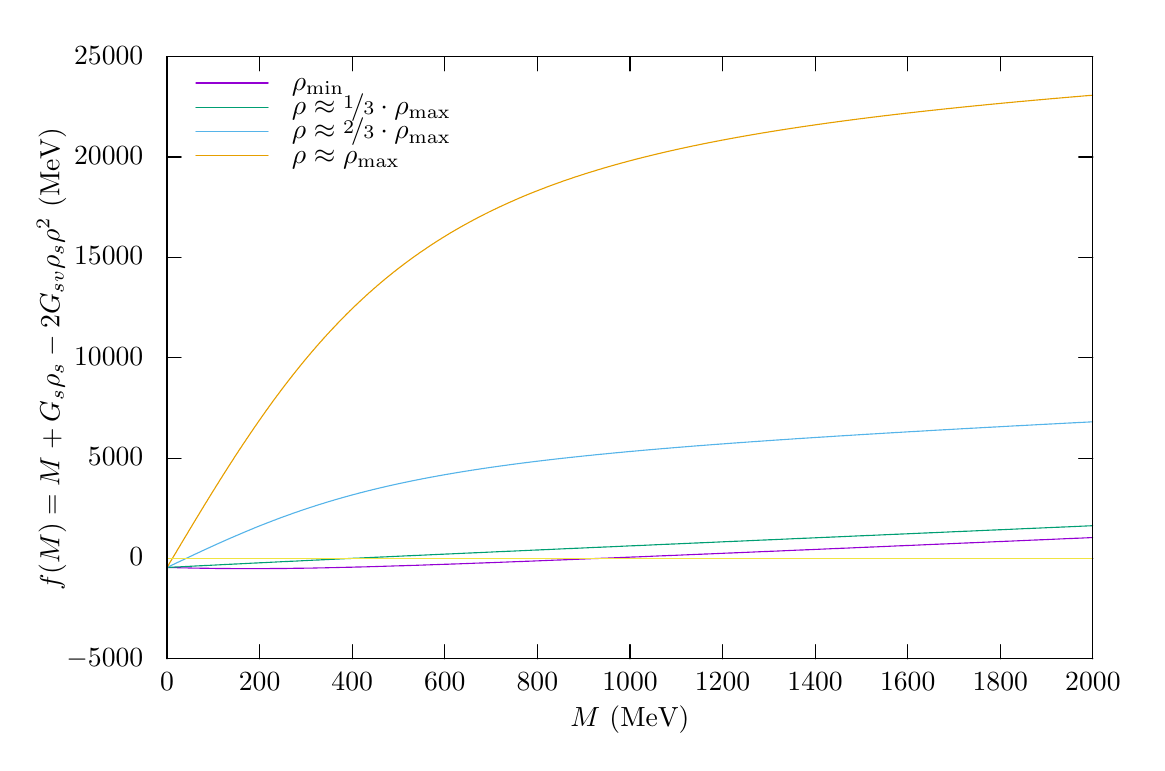
\begin{tikzpicture}[gnuplot]
%% generated with GNUPLOT 5.0p2 (Lua 5.2; terminal rev. 99, script rev. 100)
%% Fri Mar  4 16:19:36 2016
\path (0.000,0.000) rectangle (14.000,9.000);
\gpcolor{color=gp lt color border}
\gpsetlinetype{gp lt border}
\gpsetdashtype{gp dt solid}
\gpsetlinewidth{1.00}
\draw[gp path] (1.688,0.985)--(1.868,0.985);
\draw[gp path] (13.447,0.985)--(13.267,0.985);
\node[gp node right] at (1.504,0.985) {$-5000$};
\draw[gp path] (1.688,2.259)--(1.868,2.259);
\draw[gp path] (13.447,2.259)--(13.267,2.259);
\node[gp node right] at (1.504,2.259) {$0$};
\draw[gp path] (1.688,3.534)--(1.868,3.534);
\draw[gp path] (13.447,3.534)--(13.267,3.534);
\node[gp node right] at (1.504,3.534) {$5000$};
\draw[gp path] (1.688,4.808)--(1.868,4.808);
\draw[gp path] (13.447,4.808)--(13.267,4.808);
\node[gp node right] at (1.504,4.808) {$10000$};
\draw[gp path] (1.688,6.082)--(1.868,6.082);
\draw[gp path] (13.447,6.082)--(13.267,6.082);
\node[gp node right] at (1.504,6.082) {$15000$};
\draw[gp path] (1.688,7.357)--(1.868,7.357);
\draw[gp path] (13.447,7.357)--(13.267,7.357);
\node[gp node right] at (1.504,7.357) {$20000$};
\draw[gp path] (1.688,8.631)--(1.868,8.631);
\draw[gp path] (13.447,8.631)--(13.267,8.631);
\node[gp node right] at (1.504,8.631) {$25000$};
\draw[gp path] (1.688,0.985)--(1.688,1.165);
\draw[gp path] (1.688,8.631)--(1.688,8.451);
\node[gp node center] at (1.688,0.677) {$0$};
\draw[gp path] (2.864,0.985)--(2.864,1.165);
\draw[gp path] (2.864,8.631)--(2.864,8.451);
\node[gp node center] at (2.864,0.677) {$200$};
\draw[gp path] (4.040,0.985)--(4.040,1.165);
\draw[gp path] (4.040,8.631)--(4.040,8.451);
\node[gp node center] at (4.040,0.677) {$400$};
\draw[gp path] (5.216,0.985)--(5.216,1.165);
\draw[gp path] (5.216,8.631)--(5.216,8.451);
\node[gp node center] at (5.216,0.677) {$600$};
\draw[gp path] (6.392,0.985)--(6.392,1.165);
\draw[gp path] (6.392,8.631)--(6.392,8.451);
\node[gp node center] at (6.392,0.677) {$800$};
\draw[gp path] (7.568,0.985)--(7.568,1.165);
\draw[gp path] (7.568,8.631)--(7.568,8.451);
\node[gp node center] at (7.568,0.677) {$1000$};
\draw[gp path] (8.743,0.985)--(8.743,1.165);
\draw[gp path] (8.743,8.631)--(8.743,8.451);
\node[gp node center] at (8.743,0.677) {$1200$};
\draw[gp path] (9.919,0.985)--(9.919,1.165);
\draw[gp path] (9.919,8.631)--(9.919,8.451);
\node[gp node center] at (9.919,0.677) {$1400$};
\draw[gp path] (11.095,0.985)--(11.095,1.165);
\draw[gp path] (11.095,8.631)--(11.095,8.451);
\node[gp node center] at (11.095,0.677) {$1600$};
\draw[gp path] (12.271,0.985)--(12.271,1.165);
\draw[gp path] (12.271,8.631)--(12.271,8.451);
\node[gp node center] at (12.271,0.677) {$1800$};
\draw[gp path] (13.447,0.985)--(13.447,1.165);
\draw[gp path] (13.447,8.631)--(13.447,8.451);
\node[gp node center] at (13.447,0.677) {$2000$};
\draw[gp path] (1.688,8.631)--(1.688,0.985)--(13.447,0.985)--(13.447,8.631)--cycle;
\node[gp node center,rotate=-270] at (0.246,4.808) {$f(M) = M + G_s\rho_s - 2G_{sv}\rho_s\rho^2$ (MeV)};
\node[gp node center] at (7.567,0.215) {$M$ (MeV)};
\node[gp node left] at (3.156,8.297) {$\rho_{\rm{min}}$};
\gpcolor{rgb color={0.580,0.000,0.827}}
\draw[gp path] (2.056,8.297)--(2.972,8.297);
\draw[gp path] (1.691,2.145)--(1.694,2.145)--(1.697,2.144)--(1.700,2.144)--(1.703,2.144)%
  --(1.706,2.144)--(1.709,2.144)--(1.712,2.144)--(1.714,2.144)--(1.717,2.144)--(1.720,2.144)%
  --(1.723,2.144)--(1.726,2.144)--(1.729,2.144)--(1.732,2.144)--(1.735,2.144)--(1.738,2.143)%
  --(1.741,2.143)--(1.744,2.143)--(1.747,2.143)--(1.750,2.143)--(1.753,2.143)--(1.756,2.143)%
  --(1.759,2.143)--(1.761,2.143)--(1.764,2.143)--(1.767,2.143)--(1.770,2.143)--(1.773,2.143)%
  --(1.776,2.143)--(1.779,2.142)--(1.782,2.142)--(1.785,2.142)--(1.788,2.142)--(1.791,2.142)%
  --(1.794,2.142)--(1.797,2.142)--(1.800,2.142)--(1.803,2.142)--(1.806,2.142)--(1.809,2.142)%
  --(1.811,2.142)--(1.814,2.142)--(1.817,2.142)--(1.820,2.141)--(1.823,2.141)--(1.826,2.141)%
  --(1.829,2.141)--(1.832,2.141)--(1.835,2.141)--(1.838,2.141)--(1.841,2.141)--(1.844,2.141)%
  --(1.847,2.141)--(1.850,2.141)--(1.853,2.141)--(1.856,2.141)--(1.859,2.141)--(1.861,2.141)%
  --(1.864,2.140)--(1.867,2.140)--(1.870,2.140)--(1.873,2.140)--(1.876,2.140)--(1.879,2.140)%
  --(1.882,2.140)--(1.885,2.140)--(1.888,2.140)--(1.891,2.140)--(1.894,2.140)--(1.897,2.140)%
  --(1.900,2.140)--(1.903,2.140)--(1.906,2.140)--(1.908,2.139)--(1.911,2.139)--(1.914,2.139)%
  --(1.917,2.139)--(1.920,2.139)--(1.923,2.139)--(1.926,2.139)--(1.929,2.139)--(1.932,2.139)%
  --(1.935,2.139)--(1.938,2.139)--(1.941,2.139)--(1.944,2.139)--(1.947,2.139)--(1.950,2.139)%
  --(1.953,2.139)--(1.956,2.138)--(1.958,2.138)--(1.961,2.138)--(1.964,2.138)--(1.967,2.138)%
  --(1.970,2.138)--(1.973,2.138)--(1.976,2.138)--(1.979,2.138)--(1.982,2.138)--(1.985,2.138)%
  --(1.988,2.138)--(1.991,2.138)--(1.994,2.138)--(1.997,2.138)--(2.000,2.138)--(2.003,2.137)%
  --(2.005,2.137)--(2.008,2.137)--(2.011,2.137)--(2.014,2.137)--(2.017,2.137)--(2.020,2.137)%
  --(2.023,2.137)--(2.026,2.137)--(2.029,2.137)--(2.032,2.137)--(2.035,2.137)--(2.038,2.137)%
  --(2.041,2.137)--(2.044,2.137)--(2.047,2.137)--(2.050,2.137)--(2.053,2.136)--(2.055,2.136)%
  --(2.058,2.136)--(2.061,2.136)--(2.064,2.136)--(2.067,2.136)--(2.070,2.136)--(2.073,2.136)%
  --(2.076,2.136)--(2.079,2.136)--(2.082,2.136)--(2.085,2.136)--(2.088,2.136)--(2.091,2.136)%
  --(2.094,2.136)--(2.097,2.136)--(2.100,2.136)--(2.103,2.136)--(2.105,2.135)--(2.108,2.135)%
  --(2.111,2.135)--(2.114,2.135)--(2.117,2.135)--(2.120,2.135)--(2.123,2.135)--(2.126,2.135)%
  --(2.129,2.135)--(2.132,2.135)--(2.135,2.135)--(2.138,2.135)--(2.141,2.135)--(2.144,2.135)%
  --(2.147,2.135)--(2.150,2.135)--(2.152,2.135)--(2.155,2.135)--(2.158,2.135)--(2.161,2.135)%
  --(2.164,2.134)--(2.167,2.134)--(2.170,2.134)--(2.173,2.134)--(2.176,2.134)--(2.179,2.134)%
  --(2.182,2.134)--(2.185,2.134)--(2.188,2.134)--(2.191,2.134)--(2.194,2.134)--(2.197,2.134)%
  --(2.200,2.134)--(2.202,2.134)--(2.205,2.134)--(2.208,2.134)--(2.211,2.134)--(2.214,2.134)%
  --(2.217,2.134)--(2.220,2.134)--(2.223,2.134)--(2.226,2.133)--(2.229,2.133)--(2.232,2.133)%
  --(2.235,2.133)--(2.238,2.133)--(2.241,2.133)--(2.244,2.133)--(2.247,2.133)--(2.249,2.133)%
  --(2.252,2.133)--(2.255,2.133)--(2.258,2.133)--(2.261,2.133)--(2.264,2.133)--(2.267,2.133)%
  --(2.270,2.133)--(2.273,2.133)--(2.276,2.133)--(2.279,2.133)--(2.282,2.133)--(2.285,2.133)%
  --(2.288,2.133)--(2.291,2.133)--(2.294,2.133)--(2.297,2.133)--(2.299,2.132)--(2.302,2.132)%
  --(2.305,2.132)--(2.308,2.132)--(2.311,2.132)--(2.314,2.132)--(2.317,2.132)--(2.320,2.132)%
  --(2.323,2.132)--(2.326,2.132)--(2.329,2.132)--(2.332,2.132)--(2.335,2.132)--(2.338,2.132)%
  --(2.341,2.132)--(2.344,2.132)--(2.347,2.132)--(2.349,2.132)--(2.352,2.132)--(2.355,2.132)%
  --(2.358,2.132)--(2.361,2.132)--(2.364,2.132)--(2.367,2.132)--(2.370,2.132)--(2.373,2.132)%
  --(2.376,2.132)--(2.379,2.132)--(2.382,2.132)--(2.385,2.131)--(2.388,2.131)--(2.391,2.131)%
  --(2.394,2.131)--(2.396,2.131)--(2.399,2.131)--(2.402,2.131)--(2.405,2.131)--(2.408,2.131)%
  --(2.411,2.131)--(2.414,2.131)--(2.417,2.131)--(2.420,2.131)--(2.423,2.131)--(2.426,2.131)%
  --(2.429,2.131)--(2.432,2.131)--(2.435,2.131)--(2.438,2.131)--(2.441,2.131)--(2.444,2.131)%
  --(2.446,2.131)--(2.449,2.131)--(2.452,2.131)--(2.455,2.131)--(2.458,2.131)--(2.461,2.131)%
  --(2.464,2.131)--(2.467,2.131)--(2.470,2.131)--(2.473,2.131)--(2.476,2.131)--(2.479,2.131)%
  --(2.482,2.131)--(2.485,2.131)--(2.488,2.131)--(2.491,2.131)--(2.493,2.131)--(2.496,2.131)%
  --(2.499,2.130)--(2.502,2.130)--(2.505,2.130)--(2.508,2.130)--(2.511,2.130)--(2.514,2.130)%
  --(2.517,2.130)--(2.520,2.130)--(2.523,2.130)--(2.526,2.130)--(2.529,2.130)--(2.532,2.130)%
  --(2.535,2.130)--(2.538,2.130)--(2.541,2.130)--(2.543,2.130)--(2.546,2.130)--(2.549,2.130)%
  --(2.552,2.130)--(2.555,2.130)--(2.558,2.130)--(2.561,2.130)--(2.564,2.130)--(2.567,2.130)%
  --(2.570,2.130)--(2.573,2.130)--(2.576,2.130)--(2.579,2.130)--(2.582,2.130)--(2.585,2.130)%
  --(2.588,2.130)--(2.591,2.130)--(2.593,2.130)--(2.596,2.130)--(2.599,2.130)--(2.602,2.130)%
  --(2.605,2.130)--(2.608,2.130)--(2.611,2.130)--(2.614,2.130)--(2.617,2.130)--(2.620,2.130)%
  --(2.623,2.130)--(2.626,2.130)--(2.629,2.130)--(2.632,2.130)--(2.635,2.130)--(2.638,2.130)%
  --(2.640,2.130)--(2.643,2.130)--(2.646,2.130)--(2.649,2.130)--(2.652,2.130)--(2.655,2.130)%
  --(2.658,2.130)--(2.661,2.130)--(2.664,2.130)--(2.667,2.130)--(2.670,2.130)--(2.673,2.130)%
  --(2.676,2.130)--(2.679,2.130)--(2.682,2.130)--(2.685,2.130)--(2.688,2.130)--(2.690,2.130)%
  --(2.693,2.130)--(2.696,2.130)--(2.699,2.130)--(2.702,2.130)--(2.705,2.130)--(2.708,2.130)%
  --(2.711,2.130)--(2.714,2.130)--(2.717,2.130)--(2.720,2.130)--(2.723,2.130)--(2.726,2.130)%
  --(2.729,2.130)--(2.732,2.130)--(2.735,2.130)--(2.737,2.130)--(2.740,2.130)--(2.743,2.130)%
  --(2.746,2.130)--(2.749,2.130)--(2.752,2.130)--(2.755,2.130)--(2.758,2.130)--(2.761,2.130)%
  --(2.764,2.130)--(2.767,2.130)--(2.770,2.130)--(2.773,2.130)--(2.776,2.130)--(2.779,2.130)%
  --(2.782,2.130)--(2.785,2.130)--(2.787,2.130)--(2.790,2.130)--(2.793,2.130)--(2.796,2.130)%
  --(2.799,2.130)--(2.802,2.130)--(2.805,2.130)--(2.808,2.130)--(2.811,2.130)--(2.814,2.130)%
  --(2.817,2.130)--(2.820,2.130)--(2.823,2.130)--(2.826,2.130)--(2.829,2.130)--(2.832,2.130)%
  --(2.835,2.130)--(2.837,2.130)--(2.840,2.130)--(2.843,2.130)--(2.846,2.130)--(2.849,2.130)%
  --(2.852,2.130)--(2.855,2.130)--(2.858,2.130)--(2.861,2.130)--(2.864,2.130)--(2.867,2.130)%
  --(2.870,2.130)--(2.873,2.130)--(2.876,2.130)--(2.879,2.130)--(2.882,2.130)--(2.884,2.130)%
  --(2.887,2.130)--(2.890,2.130)--(2.893,2.130)--(2.896,2.130)--(2.899,2.130)--(2.902,2.130)%
  --(2.905,2.130)--(2.908,2.130)--(2.911,2.130)--(2.914,2.130)--(2.917,2.130)--(2.920,2.130)%
  --(2.923,2.130)--(2.926,2.130)--(2.929,2.130)--(2.932,2.130)--(2.934,2.130)--(2.937,2.130)%
  --(2.940,2.130)--(2.943,2.130)--(2.946,2.130)--(2.949,2.130)--(2.952,2.130)--(2.955,2.130)%
  --(2.958,2.130)--(2.961,2.130)--(2.964,2.130)--(2.967,2.130)--(2.970,2.130)--(2.973,2.130)%
  --(2.976,2.130)--(2.979,2.130)--(2.981,2.130)--(2.984,2.130)--(2.987,2.130)--(2.990,2.130)%
  --(2.993,2.130)--(2.996,2.131)--(2.999,2.131)--(3.002,2.131)--(3.005,2.131)--(3.008,2.131)%
  --(3.011,2.131)--(3.014,2.131)--(3.017,2.131)--(3.020,2.131)--(3.023,2.131)--(3.026,2.131)%
  --(3.029,2.131)--(3.031,2.131)--(3.034,2.131)--(3.037,2.131)--(3.040,2.131)--(3.043,2.131)%
  --(3.046,2.131)--(3.049,2.131)--(3.052,2.131)--(3.055,2.131)--(3.058,2.131)--(3.061,2.131)%
  --(3.064,2.131)--(3.067,2.131)--(3.070,2.131)--(3.073,2.131)--(3.076,2.131)--(3.079,2.131)%
  --(3.081,2.131)--(3.084,2.131)--(3.087,2.131)--(3.090,2.131)--(3.093,2.131)--(3.096,2.131)%
  --(3.099,2.131)--(3.102,2.131)--(3.105,2.131)--(3.108,2.131)--(3.111,2.131)--(3.114,2.131)%
  --(3.117,2.131)--(3.120,2.132)--(3.123,2.132)--(3.126,2.132)--(3.128,2.132)--(3.131,2.132)%
  --(3.134,2.132)--(3.137,2.132)--(3.140,2.132)--(3.143,2.132)--(3.146,2.132)--(3.149,2.132)%
  --(3.152,2.132)--(3.155,2.132)--(3.158,2.132)--(3.161,2.132)--(3.164,2.132)--(3.167,2.132)%
  --(3.170,2.132)--(3.173,2.132)--(3.176,2.132)--(3.178,2.132)--(3.181,2.132)--(3.184,2.132)%
  --(3.187,2.132)--(3.190,2.132)--(3.193,2.132)--(3.196,2.132)--(3.199,2.132)--(3.202,2.132)%
  --(3.205,2.132)--(3.208,2.132)--(3.211,2.132)--(3.214,2.133)--(3.217,2.133)--(3.220,2.133)%
  --(3.223,2.133)--(3.225,2.133)--(3.228,2.133)--(3.231,2.133)--(3.234,2.133)--(3.237,2.133)%
  --(3.240,2.133)--(3.243,2.133)--(3.246,2.133)--(3.249,2.133)--(3.252,2.133)--(3.255,2.133)%
  --(3.258,2.133)--(3.261,2.133)--(3.264,2.133)--(3.267,2.133)--(3.270,2.133)--(3.273,2.133)%
  --(3.275,2.133)--(3.278,2.133)--(3.281,2.133)--(3.284,2.133)--(3.287,2.133)--(3.290,2.133)%
  --(3.293,2.134)--(3.296,2.134)--(3.299,2.134)--(3.302,2.134)--(3.305,2.134)--(3.308,2.134)%
  --(3.311,2.134)--(3.314,2.134)--(3.317,2.134)--(3.320,2.134)--(3.323,2.134)--(3.325,2.134)%
  --(3.328,2.134)--(3.331,2.134)--(3.334,2.134)--(3.337,2.134)--(3.340,2.134)--(3.343,2.134)%
  --(3.346,2.134)--(3.349,2.134)--(3.352,2.134)--(3.355,2.134)--(3.358,2.134)--(3.361,2.134)%
  --(3.364,2.135)--(3.367,2.135)--(3.370,2.135)--(3.372,2.135)--(3.375,2.135)--(3.378,2.135)%
  --(3.381,2.135)--(3.384,2.135)--(3.387,2.135)--(3.390,2.135)--(3.393,2.135)--(3.396,2.135)%
  --(3.399,2.135)--(3.402,2.135)--(3.405,2.135)--(3.408,2.135)--(3.411,2.135)--(3.414,2.135)%
  --(3.417,2.135)--(3.420,2.135)--(3.422,2.135)--(3.425,2.135)--(3.428,2.136)--(3.431,2.136)%
  --(3.434,2.136)--(3.437,2.136)--(3.440,2.136)--(3.443,2.136)--(3.446,2.136)--(3.449,2.136)%
  --(3.452,2.136)--(3.455,2.136)--(3.458,2.136)--(3.461,2.136)--(3.464,2.136)--(3.467,2.136)%
  --(3.469,2.136)--(3.472,2.136)--(3.475,2.136)--(3.478,2.136)--(3.481,2.136)--(3.484,2.136)%
  --(3.487,2.137)--(3.490,2.137)--(3.493,2.137)--(3.496,2.137)--(3.499,2.137)--(3.502,2.137)%
  --(3.505,2.137)--(3.508,2.137)--(3.511,2.137)--(3.514,2.137)--(3.517,2.137)--(3.519,2.137)%
  --(3.522,2.137)--(3.525,2.137)--(3.528,2.137)--(3.531,2.137)--(3.534,2.137)--(3.537,2.137)%
  --(3.540,2.137)--(3.543,2.137)--(3.546,2.138)--(3.549,2.138)--(3.552,2.138)--(3.555,2.138)%
  --(3.558,2.138)--(3.561,2.138)--(3.564,2.138)--(3.567,2.138)--(3.569,2.138)--(3.572,2.138)%
  --(3.575,2.138)--(3.578,2.138)--(3.581,2.138)--(3.584,2.138)--(3.587,2.138)--(3.590,2.138)%
  --(3.593,2.138)--(3.596,2.138)--(3.599,2.139)--(3.602,2.139)--(3.605,2.139)--(3.608,2.139)%
  --(3.611,2.139)--(3.614,2.139)--(3.616,2.139)--(3.619,2.139)--(3.622,2.139)--(3.625,2.139)%
  --(3.628,2.139)--(3.631,2.139)--(3.634,2.139)--(3.637,2.139)--(3.640,2.139)--(3.643,2.139)%
  --(3.646,2.139)--(3.649,2.140)--(3.652,2.140)--(3.655,2.140)--(3.658,2.140)--(3.661,2.140)%
  --(3.664,2.140)--(3.666,2.140)--(3.669,2.140)--(3.672,2.140)--(3.675,2.140)--(3.678,2.140)%
  --(3.681,2.140)--(3.684,2.140)--(3.687,2.140)--(3.690,2.140)--(3.693,2.140)--(3.696,2.140)%
  --(3.699,2.141)--(3.702,2.141)--(3.705,2.141)--(3.708,2.141)--(3.711,2.141)--(3.713,2.141)%
  --(3.716,2.141)--(3.719,2.141)--(3.722,2.141)--(3.725,2.141)--(3.728,2.141)--(3.731,2.141)%
  --(3.734,2.141)--(3.737,2.141)--(3.740,2.141)--(3.743,2.141)--(3.746,2.142)--(3.749,2.142)%
  --(3.752,2.142)--(3.755,2.142)--(3.758,2.142)--(3.761,2.142)--(3.763,2.142)--(3.766,2.142)%
  --(3.769,2.142)--(3.772,2.142)--(3.775,2.142)--(3.778,2.142)--(3.781,2.142)--(3.784,2.142)%
  --(3.787,2.142)--(3.790,2.142)--(3.793,2.143)--(3.796,2.143)--(3.799,2.143)--(3.802,2.143)%
  --(3.805,2.143)--(3.808,2.143)--(3.810,2.143)--(3.813,2.143)--(3.816,2.143)--(3.819,2.143)%
  --(3.822,2.143)--(3.825,2.143)--(3.828,2.143)--(3.831,2.143)--(3.834,2.143)--(3.837,2.144)%
  --(3.840,2.144)--(3.843,2.144)--(3.846,2.144)--(3.849,2.144)--(3.852,2.144)--(3.855,2.144)%
  --(3.858,2.144)--(3.860,2.144)--(3.863,2.144)--(3.866,2.144)--(3.869,2.144)--(3.872,2.144)%
  --(3.875,2.144)--(3.878,2.145)--(3.881,2.145)--(3.884,2.145)--(3.887,2.145)--(3.890,2.145)%
  --(3.893,2.145)--(3.896,2.145)--(3.899,2.145)--(3.902,2.145)--(3.905,2.145)--(3.908,2.145)%
  --(3.910,2.145)--(3.913,2.145)--(3.916,2.145)--(3.919,2.145)--(3.922,2.146)--(3.925,2.146)%
  --(3.928,2.146)--(3.931,2.146)--(3.934,2.146)--(3.937,2.146)--(3.940,2.146)--(3.943,2.146)%
  --(3.946,2.146)--(3.949,2.146)--(3.952,2.146)--(3.955,2.146)--(3.957,2.146)--(3.960,2.146)%
  --(3.963,2.147)--(3.966,2.147)--(3.969,2.147)--(3.972,2.147)--(3.975,2.147)--(3.978,2.147)%
  --(3.981,2.147)--(3.984,2.147)--(3.987,2.147)--(3.990,2.147)--(3.993,2.147)--(3.996,2.147)%
  --(3.999,2.147)--(4.002,2.147)--(4.005,2.148)--(4.007,2.148)--(4.010,2.148)--(4.013,2.148)%
  --(4.016,2.148)--(4.019,2.148)--(4.022,2.148)--(4.025,2.148)--(4.028,2.148)--(4.031,2.148)%
  --(4.034,2.148)--(4.037,2.148)--(4.040,2.148)--(4.043,2.149)--(4.046,2.149)--(4.049,2.149)%
  --(4.052,2.149)--(4.054,2.149)--(4.057,2.149)--(4.060,2.149)--(4.063,2.149)--(4.066,2.149)%
  --(4.069,2.149)--(4.072,2.149)--(4.075,2.149)--(4.078,2.149)--(4.081,2.150)--(4.084,2.150)%
  --(4.087,2.150)--(4.090,2.150)--(4.093,2.150)--(4.096,2.150)--(4.099,2.150)--(4.102,2.150)%
  --(4.104,2.150)--(4.107,2.150)--(4.110,2.150)--(4.113,2.150)--(4.116,2.150)--(4.119,2.151)%
  --(4.122,2.151)--(4.125,2.151)--(4.128,2.151)--(4.131,2.151)--(4.134,2.151)--(4.137,2.151)%
  --(4.140,2.151)--(4.143,2.151)--(4.146,2.151)--(4.149,2.151)--(4.152,2.151)--(4.154,2.151)%
  --(4.157,2.152)--(4.160,2.152)--(4.163,2.152)--(4.166,2.152)--(4.169,2.152)--(4.172,2.152)%
  --(4.175,2.152)--(4.178,2.152)--(4.181,2.152)--(4.184,2.152)--(4.187,2.152)--(4.190,2.152)%
  --(4.193,2.152)--(4.196,2.153)--(4.199,2.153)--(4.201,2.153)--(4.204,2.153)--(4.207,2.153)%
  --(4.210,2.153)--(4.213,2.153)--(4.216,2.153)--(4.219,2.153)--(4.222,2.153)--(4.225,2.153)%
  --(4.228,2.153)--(4.231,2.154)--(4.234,2.154)--(4.237,2.154)--(4.240,2.154)--(4.243,2.154)%
  --(4.246,2.154)--(4.249,2.154)--(4.251,2.154)--(4.254,2.154)--(4.257,2.154)--(4.260,2.154)%
  --(4.263,2.154)--(4.266,2.155)--(4.269,2.155)--(4.272,2.155)--(4.275,2.155)--(4.278,2.155)%
  --(4.281,2.155)--(4.284,2.155)--(4.287,2.155)--(4.290,2.155)--(4.293,2.155)--(4.296,2.155)%
  --(4.298,2.155)--(4.301,2.156)--(4.304,2.156)--(4.307,2.156)--(4.310,2.156)--(4.313,2.156)%
  --(4.316,2.156)--(4.319,2.156)--(4.322,2.156)--(4.325,2.156)--(4.328,2.156)--(4.331,2.156)%
  --(4.334,2.156)--(4.337,2.157)--(4.340,2.157)--(4.343,2.157)--(4.346,2.157)--(4.348,2.157)%
  --(4.351,2.157)--(4.354,2.157)--(4.357,2.157)--(4.360,2.157)--(4.363,2.157)--(4.366,2.157)%
  --(4.369,2.157)--(4.372,2.158)--(4.375,2.158)--(4.378,2.158)--(4.381,2.158)--(4.384,2.158)%
  --(4.387,2.158)--(4.390,2.158)--(4.393,2.158)--(4.396,2.158)--(4.398,2.158)--(4.401,2.158)%
  --(4.404,2.158)--(4.407,2.159)--(4.410,2.159)--(4.413,2.159)--(4.416,2.159)--(4.419,2.159)%
  --(4.422,2.159)--(4.425,2.159)--(4.428,2.159)--(4.431,2.159)--(4.434,2.159)--(4.437,2.159)%
  --(4.440,2.160)--(4.443,2.160)--(4.445,2.160)--(4.448,2.160)--(4.451,2.160)--(4.454,2.160)%
  --(4.457,2.160)--(4.460,2.160)--(4.463,2.160)--(4.466,2.160)--(4.469,2.160)--(4.472,2.160)%
  --(4.475,2.161)--(4.478,2.161)--(4.481,2.161)--(4.484,2.161)--(4.487,2.161)--(4.490,2.161)%
  --(4.493,2.161)--(4.495,2.161)--(4.498,2.161)--(4.501,2.161)--(4.504,2.161)--(4.507,2.162)%
  --(4.510,2.162)--(4.513,2.162)--(4.516,2.162)--(4.519,2.162)--(4.522,2.162)--(4.525,2.162)%
  --(4.528,2.162)--(4.531,2.162)--(4.534,2.162)--(4.537,2.162)--(4.540,2.163)--(4.542,2.163)%
  --(4.545,2.163)--(4.548,2.163)--(4.551,2.163)--(4.554,2.163)--(4.557,2.163)--(4.560,2.163)%
  --(4.563,2.163)--(4.566,2.163)--(4.569,2.163)--(4.572,2.164)--(4.575,2.164)--(4.578,2.164)%
  --(4.581,2.164)--(4.584,2.164)--(4.587,2.164)--(4.590,2.164)--(4.592,2.164)--(4.595,2.164)%
  --(4.598,2.164)--(4.601,2.164)--(4.604,2.165)--(4.607,2.165)--(4.610,2.165)--(4.613,2.165)%
  --(4.616,2.165)--(4.619,2.165)--(4.622,2.165)--(4.625,2.165)--(4.628,2.165)--(4.631,2.165)%
  --(4.634,2.165)--(4.637,2.166)--(4.640,2.166)--(4.642,2.166)--(4.645,2.166)--(4.648,2.166)%
  --(4.651,2.166)--(4.654,2.166)--(4.657,2.166)--(4.660,2.166)--(4.663,2.166)--(4.666,2.166)%
  --(4.669,2.167)--(4.672,2.167)--(4.675,2.167)--(4.678,2.167)--(4.681,2.167)--(4.684,2.167)%
  --(4.687,2.167)--(4.689,2.167)--(4.692,2.167)--(4.695,2.167)--(4.698,2.167)--(4.701,2.168)%
  --(4.704,2.168)--(4.707,2.168)--(4.710,2.168)--(4.713,2.168)--(4.716,2.168)--(4.719,2.168)%
  --(4.722,2.168)--(4.725,2.168)--(4.728,2.168)--(4.731,2.169)--(4.734,2.169)--(4.737,2.169)%
  --(4.739,2.169)--(4.742,2.169)--(4.745,2.169)--(4.748,2.169)--(4.751,2.169)--(4.754,2.169)%
  --(4.757,2.169)--(4.760,2.169)--(4.763,2.170)--(4.766,2.170)--(4.769,2.170)--(4.772,2.170)%
  --(4.775,2.170)--(4.778,2.170)--(4.781,2.170)--(4.784,2.170)--(4.786,2.170)--(4.789,2.170)%
  --(4.792,2.171)--(4.795,2.171)--(4.798,2.171)--(4.801,2.171)--(4.804,2.171)--(4.807,2.171)%
  --(4.810,2.171)--(4.813,2.171)--(4.816,2.171)--(4.819,2.171)--(4.822,2.171)--(4.825,2.172)%
  --(4.828,2.172)--(4.831,2.172)--(4.834,2.172)--(4.836,2.172)--(4.839,2.172)--(4.842,2.172)%
  --(4.845,2.172)--(4.848,2.172)--(4.851,2.172)--(4.854,2.173)--(4.857,2.173)--(4.860,2.173)%
  --(4.863,2.173)--(4.866,2.173)--(4.869,2.173)--(4.872,2.173)--(4.875,2.173)--(4.878,2.173)%
  --(4.881,2.173)--(4.884,2.173)--(4.886,2.174)--(4.889,2.174)--(4.892,2.174)--(4.895,2.174)%
  --(4.898,2.174)--(4.901,2.174)--(4.904,2.174)--(4.907,2.174)--(4.910,2.174)--(4.913,2.174)%
  --(4.916,2.175)--(4.919,2.175)--(4.922,2.175)--(4.925,2.175)--(4.928,2.175)--(4.931,2.175)%
  --(4.933,2.175)--(4.936,2.175)--(4.939,2.175)--(4.942,2.175)--(4.945,2.176)--(4.948,2.176)%
  --(4.951,2.176)--(4.954,2.176)--(4.957,2.176)--(4.960,2.176)--(4.963,2.176)--(4.966,2.176)%
  --(4.969,2.176)--(4.972,2.176)--(4.975,2.177)--(4.978,2.177)--(4.981,2.177)--(4.983,2.177)%
  --(4.986,2.177)--(4.989,2.177)--(4.992,2.177)--(4.995,2.177)--(4.998,2.177)--(5.001,2.177)%
  --(5.004,2.178)--(5.007,2.178)--(5.010,2.178)--(5.013,2.178)--(5.016,2.178)--(5.019,2.178)%
  --(5.022,2.178)--(5.025,2.178)--(5.028,2.178)--(5.030,2.178)--(5.033,2.179)--(5.036,2.179)%
  --(5.039,2.179)--(5.042,2.179)--(5.045,2.179)--(5.048,2.179)--(5.051,2.179)--(5.054,2.179)%
  --(5.057,2.179)--(5.060,2.179)--(5.063,2.180)--(5.066,2.180)--(5.069,2.180)--(5.072,2.180)%
  --(5.075,2.180)--(5.078,2.180)--(5.080,2.180)--(5.083,2.180)--(5.086,2.180)--(5.089,2.180)%
  --(5.092,2.181)--(5.095,2.181)--(5.098,2.181)--(5.101,2.181)--(5.104,2.181)--(5.107,2.181)%
  --(5.110,2.181)--(5.113,2.181)--(5.116,2.181)--(5.119,2.181)--(5.122,2.182)--(5.125,2.182)%
  --(5.128,2.182)--(5.130,2.182)--(5.133,2.182)--(5.136,2.182)--(5.139,2.182)--(5.142,2.182)%
  --(5.145,2.182)--(5.148,2.182)--(5.151,2.183)--(5.154,2.183)--(5.157,2.183)--(5.160,2.183)%
  --(5.163,2.183)--(5.166,2.183)--(5.169,2.183)--(5.172,2.183)--(5.175,2.183)--(5.177,2.183)%
  --(5.180,2.184)--(5.183,2.184)--(5.186,2.184)--(5.189,2.184)--(5.192,2.184)--(5.195,2.184)%
  --(5.198,2.184)--(5.201,2.184)--(5.204,2.184)--(5.207,2.184)--(5.210,2.185)--(5.213,2.185)%
  --(5.216,2.185)--(5.219,2.185)--(5.222,2.185)--(5.225,2.185)--(5.227,2.185)--(5.230,2.185)%
  --(5.233,2.185)--(5.236,2.186)--(5.239,2.186)--(5.242,2.186)--(5.245,2.186)--(5.248,2.186)%
  --(5.251,2.186)--(5.254,2.186)--(5.257,2.186)--(5.260,2.186)--(5.263,2.186)--(5.266,2.187)%
  --(5.269,2.187)--(5.272,2.187)--(5.274,2.187)--(5.277,2.187)--(5.280,2.187)--(5.283,2.187)%
  --(5.286,2.187)--(5.289,2.187)--(5.292,2.187)--(5.295,2.188)--(5.298,2.188)--(5.301,2.188)%
  --(5.304,2.188)--(5.307,2.188)--(5.310,2.188)--(5.313,2.188)--(5.316,2.188)--(5.319,2.188)%
  --(5.322,2.189)--(5.324,2.189)--(5.327,2.189)--(5.330,2.189)--(5.333,2.189)--(5.336,2.189)%
  --(5.339,2.189)--(5.342,2.189)--(5.345,2.189)--(5.348,2.189)--(5.351,2.190)--(5.354,2.190)%
  --(5.357,2.190)--(5.360,2.190)--(5.363,2.190)--(5.366,2.190)--(5.369,2.190)--(5.372,2.190)%
  --(5.374,2.190)--(5.377,2.191)--(5.380,2.191)--(5.383,2.191)--(5.386,2.191)--(5.389,2.191)%
  --(5.392,2.191)--(5.395,2.191)--(5.398,2.191)--(5.401,2.191)--(5.404,2.191)--(5.407,2.192)%
  --(5.410,2.192)--(5.413,2.192)--(5.416,2.192)--(5.419,2.192)--(5.421,2.192)--(5.424,2.192)%
  --(5.427,2.192)--(5.430,2.192)--(5.433,2.193)--(5.436,2.193)--(5.439,2.193)--(5.442,2.193)%
  --(5.445,2.193)--(5.448,2.193)--(5.451,2.193)--(5.454,2.193)--(5.457,2.193)--(5.460,2.193)%
  --(5.463,2.194)--(5.466,2.194)--(5.469,2.194)--(5.471,2.194)--(5.474,2.194)--(5.477,2.194)%
  --(5.480,2.194)--(5.483,2.194)--(5.486,2.194)--(5.489,2.195)--(5.492,2.195)--(5.495,2.195)%
  --(5.498,2.195)--(5.501,2.195)--(5.504,2.195)--(5.507,2.195)--(5.510,2.195)--(5.513,2.195)%
  --(5.516,2.195)--(5.518,2.196)--(5.521,2.196)--(5.524,2.196)--(5.527,2.196)--(5.530,2.196)%
  --(5.533,2.196)--(5.536,2.196)--(5.539,2.196)--(5.542,2.196)--(5.545,2.197)--(5.548,2.197)%
  --(5.551,2.197)--(5.554,2.197)--(5.557,2.197)--(5.560,2.197)--(5.563,2.197)--(5.566,2.197)%
  --(5.568,2.197)--(5.571,2.198)--(5.574,2.198)--(5.577,2.198)--(5.580,2.198)--(5.583,2.198)%
  --(5.586,2.198)--(5.589,2.198)--(5.592,2.198)--(5.595,2.198)--(5.598,2.199)--(5.601,2.199)%
  --(5.604,2.199)--(5.607,2.199)--(5.610,2.199)--(5.613,2.199)--(5.616,2.199)--(5.618,2.199)%
  --(5.621,2.199)--(5.624,2.199)--(5.627,2.200)--(5.630,2.200)--(5.633,2.200)--(5.636,2.200)%
  --(5.639,2.200)--(5.642,2.200)--(5.645,2.200)--(5.648,2.200)--(5.651,2.200)--(5.654,2.201)%
  --(5.657,2.201)--(5.660,2.201)--(5.663,2.201)--(5.665,2.201)--(5.668,2.201)--(5.671,2.201)%
  --(5.674,2.201)--(5.677,2.201)--(5.680,2.202)--(5.683,2.202)--(5.686,2.202)--(5.689,2.202)%
  --(5.692,2.202)--(5.695,2.202)--(5.698,2.202)--(5.701,2.202)--(5.704,2.202)--(5.707,2.203)%
  --(5.710,2.203)--(5.713,2.203)--(5.715,2.203)--(5.718,2.203)--(5.721,2.203)--(5.724,2.203)%
  --(5.727,2.203)--(5.730,2.203)--(5.733,2.203)--(5.736,2.204)--(5.739,2.204)--(5.742,2.204)%
  --(5.745,2.204)--(5.748,2.204)--(5.751,2.204)--(5.754,2.204)--(5.757,2.204)--(5.760,2.204)%
  --(5.762,2.205)--(5.765,2.205)--(5.768,2.205)--(5.771,2.205)--(5.774,2.205)--(5.777,2.205)%
  --(5.780,2.205)--(5.783,2.205)--(5.786,2.205)--(5.789,2.206)--(5.792,2.206)--(5.795,2.206)%
  --(5.798,2.206)--(5.801,2.206)--(5.804,2.206)--(5.807,2.206)--(5.810,2.206)--(5.812,2.206)%
  --(5.815,2.207)--(5.818,2.207)--(5.821,2.207)--(5.824,2.207)--(5.827,2.207)--(5.830,2.207)%
  --(5.833,2.207)--(5.836,2.207)--(5.839,2.207)--(5.842,2.208)--(5.845,2.208)--(5.848,2.208)%
  --(5.851,2.208)--(5.854,2.208)--(5.857,2.208)--(5.860,2.208)--(5.862,2.208)--(5.865,2.208)%
  --(5.868,2.209)--(5.871,2.209)--(5.874,2.209)--(5.877,2.209)--(5.880,2.209)--(5.883,2.209)%
  --(5.886,2.209)--(5.889,2.209)--(5.892,2.209)--(5.895,2.210)--(5.898,2.210)--(5.901,2.210)%
  --(5.904,2.210)--(5.907,2.210)--(5.909,2.210)--(5.912,2.210)--(5.915,2.210)--(5.918,2.210)%
  --(5.921,2.211)--(5.924,2.211)--(5.927,2.211)--(5.930,2.211)--(5.933,2.211)--(5.936,2.211)%
  --(5.939,2.211)--(5.942,2.211)--(5.945,2.211)--(5.948,2.212)--(5.951,2.212)--(5.954,2.212)%
  --(5.957,2.212)--(5.959,2.212)--(5.962,2.212)--(5.965,2.212)--(5.968,2.212)--(5.971,2.212)%
  --(5.974,2.213)--(5.977,2.213)--(5.980,2.213)--(5.983,2.213)--(5.986,2.213)--(5.989,2.213)%
  --(5.992,2.213)--(5.995,2.213)--(5.998,2.213)--(6.001,2.214)--(6.004,2.214)--(6.006,2.214)%
  --(6.009,2.214)--(6.012,2.214)--(6.015,2.214)--(6.018,2.214)--(6.021,2.214)--(6.024,2.214)%
  --(6.027,2.215)--(6.030,2.215)--(6.033,2.215)--(6.036,2.215)--(6.039,2.215)--(6.042,2.215)%
  --(6.045,2.215)--(6.048,2.215)--(6.051,2.215)--(6.054,2.216)--(6.056,2.216)--(6.059,2.216)%
  --(6.062,2.216)--(6.065,2.216)--(6.068,2.216)--(6.071,2.216)--(6.074,2.216)--(6.077,2.216)%
  --(6.080,2.217)--(6.083,2.217)--(6.086,2.217)--(6.089,2.217)--(6.092,2.217)--(6.095,2.217)%
  --(6.098,2.217)--(6.101,2.217)--(6.104,2.217)--(6.106,2.218)--(6.109,2.218)--(6.112,2.218)%
  --(6.115,2.218)--(6.118,2.218)--(6.121,2.218)--(6.124,2.218)--(6.127,2.218)--(6.130,2.218)%
  --(6.133,2.219)--(6.136,2.219)--(6.139,2.219)--(6.142,2.219)--(6.145,2.219)--(6.148,2.219)%
  --(6.151,2.219)--(6.153,2.219)--(6.156,2.219)--(6.159,2.220)--(6.162,2.220)--(6.165,2.220)%
  --(6.168,2.220)--(6.171,2.220)--(6.174,2.220)--(6.177,2.220)--(6.180,2.220)--(6.183,2.221)%
  --(6.186,2.221)--(6.189,2.221)--(6.192,2.221)--(6.195,2.221)--(6.198,2.221)--(6.201,2.221)%
  --(6.203,2.221)--(6.206,2.221)--(6.209,2.222)--(6.212,2.222)--(6.215,2.222)--(6.218,2.222)%
  --(6.221,2.222)--(6.224,2.222)--(6.227,2.222)--(6.230,2.222)--(6.233,2.222)--(6.236,2.223)%
  --(6.239,2.223)--(6.242,2.223)--(6.245,2.223)--(6.248,2.223)--(6.250,2.223)--(6.253,2.223)%
  --(6.256,2.223)--(6.259,2.223)--(6.262,2.224)--(6.265,2.224)--(6.268,2.224)--(6.271,2.224)%
  --(6.274,2.224)--(6.277,2.224)--(6.280,2.224)--(6.283,2.224)--(6.286,2.224)--(6.289,2.225)%
  --(6.292,2.225)--(6.295,2.225)--(6.298,2.225)--(6.300,2.225)--(6.303,2.225)--(6.306,2.225)%
  --(6.309,2.225)--(6.312,2.226)--(6.315,2.226)--(6.318,2.226)--(6.321,2.226)--(6.324,2.226)%
  --(6.327,2.226)--(6.330,2.226)--(6.333,2.226)--(6.336,2.226)--(6.339,2.227)--(6.342,2.227)%
  --(6.345,2.227)--(6.348,2.227)--(6.350,2.227)--(6.353,2.227)--(6.356,2.227)--(6.359,2.227)%
  --(6.362,2.227)--(6.365,2.228)--(6.368,2.228)--(6.371,2.228)--(6.374,2.228)--(6.377,2.228)%
  --(6.380,2.228)--(6.383,2.228)--(6.386,2.228)--(6.389,2.228)--(6.392,2.229)--(6.395,2.229)%
  --(6.397,2.229)--(6.400,2.229)--(6.403,2.229)--(6.406,2.229)--(6.409,2.229)--(6.412,2.229)%
  --(6.415,2.230)--(6.418,2.230)--(6.421,2.230)--(6.424,2.230)--(6.427,2.230)--(6.430,2.230)%
  --(6.433,2.230)--(6.436,2.230)--(6.439,2.230)--(6.442,2.231)--(6.445,2.231)--(6.447,2.231)%
  --(6.450,2.231)--(6.453,2.231)--(6.456,2.231)--(6.459,2.231)--(6.462,2.231)--(6.465,2.231)%
  --(6.468,2.232)--(6.471,2.232)--(6.474,2.232)--(6.477,2.232)--(6.480,2.232)--(6.483,2.232)%
  --(6.486,2.232)--(6.489,2.232)--(6.492,2.233)--(6.494,2.233)--(6.497,2.233)--(6.500,2.233)%
  --(6.503,2.233)--(6.506,2.233)--(6.509,2.233)--(6.512,2.233)--(6.515,2.233)--(6.518,2.234)%
  --(6.521,2.234)--(6.524,2.234)--(6.527,2.234)--(6.530,2.234)--(6.533,2.234)--(6.536,2.234)%
  --(6.539,2.234)--(6.542,2.234)--(6.544,2.235)--(6.547,2.235)--(6.550,2.235)--(6.553,2.235)%
  --(6.556,2.235)--(6.559,2.235)--(6.562,2.235)--(6.565,2.235)--(6.568,2.236)--(6.571,2.236)%
  --(6.574,2.236)--(6.577,2.236)--(6.580,2.236)--(6.583,2.236)--(6.586,2.236)--(6.589,2.236)%
  --(6.592,2.236)--(6.594,2.237)--(6.597,2.237)--(6.600,2.237)--(6.603,2.237)--(6.606,2.237)%
  --(6.609,2.237)--(6.612,2.237)--(6.615,2.237)--(6.618,2.237)--(6.621,2.238)--(6.624,2.238)%
  --(6.627,2.238)--(6.630,2.238)--(6.633,2.238)--(6.636,2.238)--(6.639,2.238)--(6.641,2.238)%
  --(6.644,2.239)--(6.647,2.239)--(6.650,2.239)--(6.653,2.239)--(6.656,2.239)--(6.659,2.239)%
  --(6.662,2.239)--(6.665,2.239)--(6.668,2.239)--(6.671,2.240)--(6.674,2.240)--(6.677,2.240)%
  --(6.680,2.240)--(6.683,2.240)--(6.686,2.240)--(6.689,2.240)--(6.691,2.240)--(6.694,2.240)%
  --(6.697,2.241)--(6.700,2.241)--(6.703,2.241)--(6.706,2.241)--(6.709,2.241)--(6.712,2.241)%
  --(6.715,2.241)--(6.718,2.241)--(6.721,2.242)--(6.724,2.242)--(6.727,2.242)--(6.730,2.242)%
  --(6.733,2.242)--(6.736,2.242)--(6.738,2.242)--(6.741,2.242)--(6.744,2.242)--(6.747,2.243)%
  --(6.750,2.243)--(6.753,2.243)--(6.756,2.243)--(6.759,2.243)--(6.762,2.243)--(6.765,2.243)%
  --(6.768,2.243)--(6.771,2.244)--(6.774,2.244)--(6.777,2.244)--(6.780,2.244)--(6.783,2.244)%
  --(6.786,2.244)--(6.788,2.244)--(6.791,2.244)--(6.794,2.244)--(6.797,2.245)--(6.800,2.245)%
  --(6.803,2.245)--(6.806,2.245)--(6.809,2.245)--(6.812,2.245)--(6.815,2.245)--(6.818,2.245)%
  --(6.821,2.246)--(6.824,2.246)--(6.827,2.246)--(6.830,2.246)--(6.833,2.246)--(6.836,2.246)%
  --(6.838,2.246)--(6.841,2.246)--(6.844,2.246)--(6.847,2.247)--(6.850,2.247)--(6.853,2.247)%
  --(6.856,2.247)--(6.859,2.247)--(6.862,2.247)--(6.865,2.247)--(6.868,2.247)--(6.871,2.248)%
  --(6.874,2.248)--(6.877,2.248)--(6.880,2.248)--(6.883,2.248)--(6.885,2.248)--(6.888,2.248)%
  --(6.891,2.248)--(6.894,2.248)--(6.897,2.249)--(6.900,2.249)--(6.903,2.249)--(6.906,2.249)%
  --(6.909,2.249)--(6.912,2.249)--(6.915,2.249)--(6.918,2.249)--(6.921,2.250)--(6.924,2.250)%
  --(6.927,2.250)--(6.930,2.250)--(6.933,2.250)--(6.935,2.250)--(6.938,2.250)--(6.941,2.250)%
  --(6.944,2.250)--(6.947,2.251)--(6.950,2.251)--(6.953,2.251)--(6.956,2.251)--(6.959,2.251)%
  --(6.962,2.251)--(6.965,2.251)--(6.968,2.251)--(6.971,2.252)--(6.974,2.252)--(6.977,2.252)%
  --(6.980,2.252)--(6.982,2.252)--(6.985,2.252)--(6.988,2.252)--(6.991,2.252)--(6.994,2.252)%
  --(6.997,2.253)--(7.000,2.253)--(7.003,2.253)--(7.006,2.253)--(7.009,2.253)--(7.012,2.253)%
  --(7.015,2.253)--(7.018,2.253)--(7.021,2.254)--(7.024,2.254)--(7.027,2.254)--(7.030,2.254)%
  --(7.032,2.254)--(7.035,2.254)--(7.038,2.254)--(7.041,2.254)--(7.044,2.254)--(7.047,2.255)%
  --(7.050,2.255)--(7.053,2.255)--(7.056,2.255)--(7.059,2.255)--(7.062,2.255)--(7.065,2.255)%
  --(7.068,2.255)--(7.071,2.256)--(7.074,2.256)--(7.077,2.256)--(7.080,2.256)--(7.082,2.256)%
  --(7.085,2.256)--(7.088,2.256)--(7.091,2.256)--(7.094,2.256)--(7.097,2.257)--(7.100,2.257)%
  --(7.103,2.257)--(7.106,2.257)--(7.109,2.257)--(7.112,2.257)--(7.115,2.257)--(7.118,2.257)%
  --(7.121,2.258)--(7.124,2.258)--(7.127,2.258)--(7.129,2.258)--(7.132,2.258)--(7.135,2.258)%
  --(7.138,2.258)--(7.141,2.258)--(7.144,2.258)--(7.147,2.259)--(7.150,2.259)--(7.153,2.259)%
  --(7.156,2.259)--(7.159,2.259)--(7.162,2.259)--(7.165,2.259)--(7.168,2.259)--(7.171,2.260)%
  --(7.174,2.260)--(7.177,2.260)--(7.179,2.260)--(7.182,2.260)--(7.185,2.260)--(7.188,2.260)%
  --(7.191,2.260)--(7.194,2.260)--(7.197,2.261)--(7.200,2.261)--(7.203,2.261)--(7.206,2.261)%
  --(7.209,2.261)--(7.212,2.261)--(7.215,2.261)--(7.218,2.261)--(7.221,2.262)--(7.224,2.262)%
  --(7.226,2.262)--(7.229,2.262)--(7.232,2.262)--(7.235,2.262)--(7.238,2.262)--(7.241,2.262)%
  --(7.244,2.263)--(7.247,2.263)--(7.250,2.263)--(7.253,2.263)--(7.256,2.263)--(7.259,2.263)%
  --(7.262,2.263)--(7.265,2.263)--(7.268,2.263)--(7.271,2.264)--(7.274,2.264)--(7.276,2.264)%
  --(7.279,2.264)--(7.282,2.264)--(7.285,2.264)--(7.288,2.264)--(7.291,2.264)--(7.294,2.265)%
  --(7.297,2.265)--(7.300,2.265)--(7.303,2.265)--(7.306,2.265)--(7.309,2.265)--(7.312,2.265)%
  --(7.315,2.265)--(7.318,2.265)--(7.321,2.266)--(7.324,2.266)--(7.326,2.266)--(7.329,2.266)%
  --(7.332,2.266)--(7.335,2.266)--(7.338,2.266)--(7.341,2.266)--(7.344,2.267)--(7.347,2.267)%
  --(7.350,2.267)--(7.353,2.267)--(7.356,2.267)--(7.359,2.267)--(7.362,2.267)--(7.365,2.267)%
  --(7.368,2.268)--(7.371,2.268)--(7.373,2.268)--(7.376,2.268)--(7.379,2.268)--(7.382,2.268)%
  --(7.385,2.268)--(7.388,2.268)--(7.391,2.268)--(7.394,2.269)--(7.397,2.269)--(7.400,2.269)%
  --(7.403,2.269)--(7.406,2.269)--(7.409,2.269)--(7.412,2.269)--(7.415,2.269)--(7.418,2.270)%
  --(7.421,2.270)--(7.423,2.270)--(7.426,2.270)--(7.429,2.270)--(7.432,2.270)--(7.435,2.270)%
  --(7.438,2.270)--(7.441,2.271)--(7.444,2.271)--(7.447,2.271)--(7.450,2.271)--(7.453,2.271)%
  --(7.456,2.271)--(7.459,2.271)--(7.462,2.271)--(7.465,2.271)--(7.468,2.272)--(7.470,2.272)%
  --(7.473,2.272)--(7.476,2.272)--(7.479,2.272)--(7.482,2.272)--(7.485,2.272)--(7.488,2.272)%
  --(7.491,2.273)--(7.494,2.273)--(7.497,2.273)--(7.500,2.273)--(7.503,2.273)--(7.506,2.273)%
  --(7.509,2.273)--(7.512,2.273)--(7.515,2.274)--(7.518,2.274)--(7.520,2.274)--(7.523,2.274)%
  --(7.526,2.274)--(7.529,2.274)--(7.532,2.274)--(7.535,2.274)--(7.538,2.274)--(7.541,2.275)%
  --(7.544,2.275)--(7.547,2.275)--(7.550,2.275)--(7.553,2.275)--(7.556,2.275)--(7.559,2.275)%
  --(7.562,2.275)--(7.565,2.276)--(7.568,2.276)--(7.570,2.276)--(7.573,2.276)--(7.576,2.276)%
  --(7.579,2.276)--(7.582,2.276)--(7.585,2.276)--(7.588,2.277)--(7.591,2.277)--(7.594,2.277)%
  --(7.597,2.277)--(7.600,2.277)--(7.603,2.277)--(7.606,2.277)--(7.609,2.277)--(7.612,2.277)%
  --(7.615,2.278)--(7.617,2.278)--(7.620,2.278)--(7.623,2.278)--(7.626,2.278)--(7.629,2.278)%
  --(7.632,2.278)--(7.635,2.278)--(7.638,2.279)--(7.641,2.279)--(7.644,2.279)--(7.647,2.279)%
  --(7.650,2.279)--(7.653,2.279)--(7.656,2.279)--(7.659,2.279)--(7.662,2.280)--(7.665,2.280)%
  --(7.667,2.280)--(7.670,2.280)--(7.673,2.280)--(7.676,2.280)--(7.679,2.280)--(7.682,2.280)%
  --(7.685,2.280)--(7.688,2.281)--(7.691,2.281)--(7.694,2.281)--(7.697,2.281)--(7.700,2.281)%
  --(7.703,2.281)--(7.706,2.281)--(7.709,2.281)--(7.712,2.282)--(7.714,2.282)--(7.717,2.282)%
  --(7.720,2.282)--(7.723,2.282)--(7.726,2.282)--(7.729,2.282)--(7.732,2.282)--(7.735,2.283)%
  --(7.738,2.283)--(7.741,2.283)--(7.744,2.283)--(7.747,2.283)--(7.750,2.283)--(7.753,2.283)%
  --(7.756,2.283)--(7.759,2.283)--(7.762,2.284)--(7.764,2.284)--(7.767,2.284)--(7.770,2.284)%
  --(7.773,2.284)--(7.776,2.284)--(7.779,2.284)--(7.782,2.284)--(7.785,2.285)--(7.788,2.285)%
  --(7.791,2.285)--(7.794,2.285)--(7.797,2.285)--(7.800,2.285)--(7.803,2.285)--(7.806,2.285)%
  --(7.809,2.286)--(7.811,2.286)--(7.814,2.286)--(7.817,2.286)--(7.820,2.286)--(7.823,2.286)%
  --(7.826,2.286)--(7.829,2.286)--(7.832,2.287)--(7.835,2.287)--(7.838,2.287)--(7.841,2.287)%
  --(7.844,2.287)--(7.847,2.287)--(7.850,2.287)--(7.853,2.287)--(7.856,2.287)--(7.859,2.288)%
  --(7.861,2.288)--(7.864,2.288)--(7.867,2.288)--(7.870,2.288)--(7.873,2.288)--(7.876,2.288)%
  --(7.879,2.288)--(7.882,2.289)--(7.885,2.289)--(7.888,2.289)--(7.891,2.289)--(7.894,2.289)%
  --(7.897,2.289)--(7.900,2.289)--(7.903,2.289)--(7.906,2.290)--(7.909,2.290)--(7.911,2.290)%
  --(7.914,2.290)--(7.917,2.290)--(7.920,2.290)--(7.923,2.290)--(7.926,2.290)--(7.929,2.291)%
  --(7.932,2.291)--(7.935,2.291)--(7.938,2.291)--(7.941,2.291)--(7.944,2.291)--(7.947,2.291)%
  --(7.950,2.291)--(7.953,2.291)--(7.956,2.292)--(7.958,2.292)--(7.961,2.292)--(7.964,2.292)%
  --(7.967,2.292)--(7.970,2.292)--(7.973,2.292)--(7.976,2.292)--(7.979,2.293)--(7.982,2.293)%
  --(7.985,2.293)--(7.988,2.293)--(7.991,2.293)--(7.994,2.293)--(7.997,2.293)--(8.000,2.293)%
  --(8.003,2.294)--(8.006,2.294)--(8.008,2.294)--(8.011,2.294)--(8.014,2.294)--(8.017,2.294)%
  --(8.020,2.294)--(8.023,2.294)--(8.026,2.295)--(8.029,2.295)--(8.032,2.295)--(8.035,2.295)%
  --(8.038,2.295)--(8.041,2.295)--(8.044,2.295)--(8.047,2.295)--(8.050,2.295)--(8.053,2.296)%
  --(8.055,2.296)--(8.058,2.296)--(8.061,2.296)--(8.064,2.296)--(8.067,2.296)--(8.070,2.296)%
  --(8.073,2.296)--(8.076,2.297)--(8.079,2.297)--(8.082,2.297)--(8.085,2.297)--(8.088,2.297)%
  --(8.091,2.297)--(8.094,2.297)--(8.097,2.297)--(8.100,2.298)--(8.103,2.298)--(8.105,2.298)%
  --(8.108,2.298)--(8.111,2.298)--(8.114,2.298)--(8.117,2.298)--(8.120,2.298)--(8.123,2.299)%
  --(8.126,2.299)--(8.129,2.299)--(8.132,2.299)--(8.135,2.299)--(8.138,2.299)--(8.141,2.299)%
  --(8.144,2.299)--(8.147,2.299)--(8.150,2.300)--(8.153,2.300)--(8.155,2.300)--(8.158,2.300)%
  --(8.161,2.300)--(8.164,2.300)--(8.167,2.300)--(8.170,2.300)--(8.173,2.301)--(8.176,2.301)%
  --(8.179,2.301)--(8.182,2.301)--(8.185,2.301)--(8.188,2.301)--(8.191,2.301)--(8.194,2.301)%
  --(8.197,2.302)--(8.200,2.302)--(8.202,2.302)--(8.205,2.302)--(8.208,2.302)--(8.211,2.302)%
  --(8.214,2.302)--(8.217,2.302)--(8.220,2.303)--(8.223,2.303)--(8.226,2.303)--(8.229,2.303)%
  --(8.232,2.303)--(8.235,2.303)--(8.238,2.303)--(8.241,2.303)--(8.244,2.304)--(8.247,2.304)%
  --(8.250,2.304)--(8.252,2.304)--(8.255,2.304)--(8.258,2.304)--(8.261,2.304)--(8.264,2.304)%
  --(8.267,2.304)--(8.270,2.305)--(8.273,2.305)--(8.276,2.305)--(8.279,2.305)--(8.282,2.305)%
  --(8.285,2.305)--(8.288,2.305)--(8.291,2.305)--(8.294,2.306)--(8.297,2.306)--(8.299,2.306)%
  --(8.302,2.306)--(8.305,2.306)--(8.308,2.306)--(8.311,2.306)--(8.314,2.306)--(8.317,2.307)%
  --(8.320,2.307)--(8.323,2.307)--(8.326,2.307)--(8.329,2.307)--(8.332,2.307)--(8.335,2.307)%
  --(8.338,2.307)--(8.341,2.308)--(8.344,2.308)--(8.347,2.308)--(8.349,2.308)--(8.352,2.308)%
  --(8.355,2.308)--(8.358,2.308)--(8.361,2.308)--(8.364,2.309)--(8.367,2.309)--(8.370,2.309)%
  --(8.373,2.309)--(8.376,2.309)--(8.379,2.309)--(8.382,2.309)--(8.385,2.309)--(8.388,2.309)%
  --(8.391,2.310)--(8.394,2.310)--(8.397,2.310)--(8.399,2.310)--(8.402,2.310)--(8.405,2.310)%
  --(8.408,2.310)--(8.411,2.310)--(8.414,2.311)--(8.417,2.311)--(8.420,2.311)--(8.423,2.311)%
  --(8.426,2.311)--(8.429,2.311)--(8.432,2.311)--(8.435,2.311)--(8.438,2.312)--(8.441,2.312)%
  --(8.444,2.312)--(8.446,2.312)--(8.449,2.312)--(8.452,2.312)--(8.455,2.312)--(8.458,2.312)%
  --(8.461,2.313)--(8.464,2.313)--(8.467,2.313)--(8.470,2.313)--(8.473,2.313)--(8.476,2.313)%
  --(8.479,2.313)--(8.482,2.313)--(8.485,2.314)--(8.488,2.314)--(8.491,2.314)--(8.494,2.314)%
  --(8.496,2.314)--(8.499,2.314)--(8.502,2.314)--(8.505,2.314)--(8.508,2.315)--(8.511,2.315)%
  --(8.514,2.315)--(8.517,2.315)--(8.520,2.315)--(8.523,2.315)--(8.526,2.315)--(8.529,2.315)%
  --(8.532,2.315)--(8.535,2.316)--(8.538,2.316)--(8.541,2.316)--(8.543,2.316)--(8.546,2.316)%
  --(8.549,2.316)--(8.552,2.316)--(8.555,2.316)--(8.558,2.317)--(8.561,2.317)--(8.564,2.317)%
  --(8.567,2.317)--(8.570,2.317)--(8.573,2.317)--(8.576,2.317)--(8.579,2.317)--(8.582,2.318)%
  --(8.585,2.318)--(8.588,2.318)--(8.591,2.318)--(8.593,2.318)--(8.596,2.318)--(8.599,2.318)%
  --(8.602,2.318)--(8.605,2.319)--(8.608,2.319)--(8.611,2.319)--(8.614,2.319)--(8.617,2.319)%
  --(8.620,2.319)--(8.623,2.319)--(8.626,2.319)--(8.629,2.320)--(8.632,2.320)--(8.635,2.320)%
  --(8.638,2.320)--(8.641,2.320)--(8.643,2.320)--(8.646,2.320)--(8.649,2.320)--(8.652,2.321)%
  --(8.655,2.321)--(8.658,2.321)--(8.661,2.321)--(8.664,2.321)--(8.667,2.321)--(8.670,2.321)%
  --(8.673,2.321)--(8.676,2.321)--(8.679,2.322)--(8.682,2.322)--(8.685,2.322)--(8.688,2.322)%
  --(8.690,2.322)--(8.693,2.322)--(8.696,2.322)--(8.699,2.322)--(8.702,2.323)--(8.705,2.323)%
  --(8.708,2.323)--(8.711,2.323)--(8.714,2.323)--(8.717,2.323)--(8.720,2.323)--(8.723,2.323)%
  --(8.726,2.324)--(8.729,2.324)--(8.732,2.324)--(8.735,2.324)--(8.738,2.324)--(8.740,2.324)%
  --(8.743,2.324)--(8.746,2.324)--(8.749,2.325)--(8.752,2.325)--(8.755,2.325)--(8.758,2.325)%
  --(8.761,2.325)--(8.764,2.325)--(8.767,2.325)--(8.770,2.325)--(8.773,2.326)--(8.776,2.326)%
  --(8.779,2.326)--(8.782,2.326)--(8.785,2.326)--(8.787,2.326)--(8.790,2.326)--(8.793,2.326)%
  --(8.796,2.327)--(8.799,2.327)--(8.802,2.327)--(8.805,2.327)--(8.808,2.327)--(8.811,2.327)%
  --(8.814,2.327)--(8.817,2.327)--(8.820,2.328)--(8.823,2.328)--(8.826,2.328)--(8.829,2.328)%
  --(8.832,2.328)--(8.835,2.328)--(8.837,2.328)--(8.840,2.328)--(8.843,2.329)--(8.846,2.329)%
  --(8.849,2.329)--(8.852,2.329)--(8.855,2.329)--(8.858,2.329)--(8.861,2.329)--(8.864,2.329)%
  --(8.867,2.329)--(8.870,2.330)--(8.873,2.330)--(8.876,2.330)--(8.879,2.330)--(8.882,2.330)%
  --(8.885,2.330)--(8.887,2.330)--(8.890,2.330)--(8.893,2.331)--(8.896,2.331)--(8.899,2.331)%
  --(8.902,2.331)--(8.905,2.331)--(8.908,2.331)--(8.911,2.331)--(8.914,2.331)--(8.917,2.332)%
  --(8.920,2.332)--(8.923,2.332)--(8.926,2.332)--(8.929,2.332)--(8.932,2.332)--(8.934,2.332)%
  --(8.937,2.332)--(8.940,2.333)--(8.943,2.333)--(8.946,2.333)--(8.949,2.333)--(8.952,2.333)%
  --(8.955,2.333)--(8.958,2.333)--(8.961,2.333)--(8.964,2.334)--(8.967,2.334)--(8.970,2.334)%
  --(8.973,2.334)--(8.976,2.334)--(8.979,2.334)--(8.982,2.334)--(8.984,2.334)--(8.987,2.335)%
  --(8.990,2.335)--(8.993,2.335)--(8.996,2.335)--(8.999,2.335)--(9.002,2.335)--(9.005,2.335)%
  --(9.008,2.335)--(9.011,2.336)--(9.014,2.336)--(9.017,2.336)--(9.020,2.336)--(9.023,2.336)%
  --(9.026,2.336)--(9.029,2.336)--(9.031,2.336)--(9.034,2.337)--(9.037,2.337)--(9.040,2.337)%
  --(9.043,2.337)--(9.046,2.337)--(9.049,2.337)--(9.052,2.337)--(9.055,2.337)--(9.058,2.338)%
  --(9.061,2.338)--(9.064,2.338)--(9.067,2.338)--(9.070,2.338)--(9.073,2.338)--(9.076,2.338)%
  --(9.079,2.338)--(9.081,2.338)--(9.084,2.339)--(9.087,2.339)--(9.090,2.339)--(9.093,2.339)%
  --(9.096,2.339)--(9.099,2.339)--(9.102,2.339)--(9.105,2.339)--(9.108,2.340)--(9.111,2.340)%
  --(9.114,2.340)--(9.117,2.340)--(9.120,2.340)--(9.123,2.340)--(9.126,2.340)--(9.129,2.340)%
  --(9.131,2.341)--(9.134,2.341)--(9.137,2.341)--(9.140,2.341)--(9.143,2.341)--(9.146,2.341)%
  --(9.149,2.341)--(9.152,2.341)--(9.155,2.342)--(9.158,2.342)--(9.161,2.342)--(9.164,2.342)%
  --(9.167,2.342)--(9.170,2.342)--(9.173,2.342)--(9.176,2.342)--(9.178,2.343)--(9.181,2.343)%
  --(9.184,2.343)--(9.187,2.343)--(9.190,2.343)--(9.193,2.343)--(9.196,2.343)--(9.199,2.343)%
  --(9.202,2.344)--(9.205,2.344)--(9.208,2.344)--(9.211,2.344)--(9.214,2.344)--(9.217,2.344)%
  --(9.220,2.344)--(9.223,2.344)--(9.226,2.345)--(9.228,2.345)--(9.231,2.345)--(9.234,2.345)%
  --(9.237,2.345)--(9.240,2.345)--(9.243,2.345)--(9.246,2.345)--(9.249,2.346)--(9.252,2.346)%
  --(9.255,2.346)--(9.258,2.346)--(9.261,2.346)--(9.264,2.346)--(9.267,2.346)--(9.270,2.346)%
  --(9.273,2.347)--(9.275,2.347)--(9.278,2.347)--(9.281,2.347)--(9.284,2.347)--(9.287,2.347)%
  --(9.290,2.347)--(9.293,2.347)--(9.296,2.348)--(9.299,2.348)--(9.302,2.348)--(9.305,2.348)%
  --(9.308,2.348)--(9.311,2.348)--(9.314,2.348)--(9.317,2.348)--(9.320,2.349)--(9.323,2.349)%
  --(9.325,2.349)--(9.328,2.349)--(9.331,2.349)--(9.334,2.349)--(9.337,2.349)--(9.340,2.349)%
  --(9.343,2.349)--(9.346,2.350)--(9.349,2.350)--(9.352,2.350)--(9.355,2.350)--(9.358,2.350)%
  --(9.361,2.350)--(9.364,2.350)--(9.367,2.350)--(9.370,2.351)--(9.373,2.351)--(9.375,2.351)%
  --(9.378,2.351)--(9.381,2.351)--(9.384,2.351)--(9.387,2.351)--(9.390,2.351)--(9.393,2.352)%
  --(9.396,2.352)--(9.399,2.352)--(9.402,2.352)--(9.405,2.352)--(9.408,2.352)--(9.411,2.352)%
  --(9.414,2.352)--(9.417,2.353)--(9.420,2.353)--(9.422,2.353)--(9.425,2.353)--(9.428,2.353)%
  --(9.431,2.353)--(9.434,2.353)--(9.437,2.353)--(9.440,2.354)--(9.443,2.354)--(9.446,2.354)%
  --(9.449,2.354)--(9.452,2.354)--(9.455,2.354)--(9.458,2.354)--(9.461,2.354)--(9.464,2.355)%
  --(9.467,2.355)--(9.470,2.355)--(9.472,2.355)--(9.475,2.355)--(9.478,2.355)--(9.481,2.355)%
  --(9.484,2.355)--(9.487,2.356)--(9.490,2.356)--(9.493,2.356)--(9.496,2.356)--(9.499,2.356)%
  --(9.502,2.356)--(9.505,2.356)--(9.508,2.356)--(9.511,2.357)--(9.514,2.357)--(9.517,2.357)%
  --(9.519,2.357)--(9.522,2.357)--(9.525,2.357)--(9.528,2.357)--(9.531,2.357)--(9.534,2.358)%
  --(9.537,2.358)--(9.540,2.358)--(9.543,2.358)--(9.546,2.358)--(9.549,2.358)--(9.552,2.358)%
  --(9.555,2.358)--(9.558,2.359)--(9.561,2.359)--(9.564,2.359)--(9.567,2.359)--(9.569,2.359)%
  --(9.572,2.359)--(9.575,2.359)--(9.578,2.359)--(9.581,2.360)--(9.584,2.360)--(9.587,2.360)%
  --(9.590,2.360)--(9.593,2.360)--(9.596,2.360)--(9.599,2.360)--(9.602,2.360)--(9.605,2.361)%
  --(9.608,2.361)--(9.611,2.361)--(9.614,2.361)--(9.617,2.361)--(9.619,2.361)--(9.622,2.361)%
  --(9.625,2.361)--(9.628,2.362)--(9.631,2.362)--(9.634,2.362)--(9.637,2.362)--(9.640,2.362)%
  --(9.643,2.362)--(9.646,2.362)--(9.649,2.362)--(9.652,2.363)--(9.655,2.363)--(9.658,2.363)%
  --(9.661,2.363)--(9.664,2.363)--(9.666,2.363)--(9.669,2.363)--(9.672,2.363)--(9.675,2.364)%
  --(9.678,2.364)--(9.681,2.364)--(9.684,2.364)--(9.687,2.364)--(9.690,2.364)--(9.693,2.364)%
  --(9.696,2.364)--(9.699,2.364)--(9.702,2.365)--(9.705,2.365)--(9.708,2.365)--(9.711,2.365)%
  --(9.714,2.365)--(9.716,2.365)--(9.719,2.365)--(9.722,2.365)--(9.725,2.366)--(9.728,2.366)%
  --(9.731,2.366)--(9.734,2.366)--(9.737,2.366)--(9.740,2.366)--(9.743,2.366)--(9.746,2.366)%
  --(9.749,2.367)--(9.752,2.367)--(9.755,2.367)--(9.758,2.367)--(9.761,2.367)--(9.763,2.367)%
  --(9.766,2.367)--(9.769,2.367)--(9.772,2.368)--(9.775,2.368)--(9.778,2.368)--(9.781,2.368)%
  --(9.784,2.368)--(9.787,2.368)--(9.790,2.368)--(9.793,2.368)--(9.796,2.369)--(9.799,2.369)%
  --(9.802,2.369)--(9.805,2.369)--(9.808,2.369)--(9.811,2.369)--(9.813,2.369)--(9.816,2.369)%
  --(9.819,2.370)--(9.822,2.370)--(9.825,2.370)--(9.828,2.370)--(9.831,2.370)--(9.834,2.370)%
  --(9.837,2.370)--(9.840,2.370)--(9.843,2.371)--(9.846,2.371)--(9.849,2.371)--(9.852,2.371)%
  --(9.855,2.371)--(9.858,2.371)--(9.861,2.371)--(9.863,2.371)--(9.866,2.372)--(9.869,2.372)%
  --(9.872,2.372)--(9.875,2.372)--(9.878,2.372)--(9.881,2.372)--(9.884,2.372)--(9.887,2.372)%
  --(9.890,2.373)--(9.893,2.373)--(9.896,2.373)--(9.899,2.373)--(9.902,2.373)--(9.905,2.373)%
  --(9.908,2.373)--(9.910,2.373)--(9.913,2.374)--(9.916,2.374)--(9.919,2.374)--(9.922,2.374)%
  --(9.925,2.374)--(9.928,2.374)--(9.931,2.374)--(9.934,2.374)--(9.937,2.375)--(9.940,2.375)%
  --(9.943,2.375)--(9.946,2.375)--(9.949,2.375)--(9.952,2.375)--(9.955,2.375)--(9.958,2.375)%
  --(9.960,2.376)--(9.963,2.376)--(9.966,2.376)--(9.969,2.376)--(9.972,2.376)--(9.975,2.376)%
  --(9.978,2.376)--(9.981,2.376)--(9.984,2.377)--(9.987,2.377)--(9.990,2.377)--(9.993,2.377)%
  --(9.996,2.377)--(9.999,2.377)--(10.002,2.377)--(10.005,2.377)--(10.007,2.378)--(10.010,2.378)%
  --(10.013,2.378)--(10.016,2.378)--(10.019,2.378)--(10.022,2.378)--(10.025,2.378)--(10.028,2.378)%
  --(10.031,2.379)--(10.034,2.379)--(10.037,2.379)--(10.040,2.379)--(10.043,2.379)--(10.046,2.379)%
  --(10.049,2.379)--(10.052,2.379)--(10.055,2.380)--(10.057,2.380)--(10.060,2.380)--(10.063,2.380)%
  --(10.066,2.380)--(10.069,2.380)--(10.072,2.380)--(10.075,2.380)--(10.078,2.381)--(10.081,2.381)%
  --(10.084,2.381)--(10.087,2.381)--(10.090,2.381)--(10.093,2.381)--(10.096,2.381)--(10.099,2.381)%
  --(10.102,2.382)--(10.105,2.382)--(10.107,2.382)--(10.110,2.382)--(10.113,2.382)--(10.116,2.382)%
  --(10.119,2.382)--(10.122,2.382)--(10.125,2.383)--(10.128,2.383)--(10.131,2.383)--(10.134,2.383)%
  --(10.137,2.383)--(10.140,2.383)--(10.143,2.383)--(10.146,2.383)--(10.149,2.384)--(10.152,2.384)%
  --(10.154,2.384)--(10.157,2.384)--(10.160,2.384)--(10.163,2.384)--(10.166,2.384)--(10.169,2.384)%
  --(10.172,2.385)--(10.175,2.385)--(10.178,2.385)--(10.181,2.385)--(10.184,2.385)--(10.187,2.385)%
  --(10.190,2.385)--(10.193,2.385)--(10.196,2.386)--(10.199,2.386)--(10.202,2.386)--(10.204,2.386)%
  --(10.207,2.386)--(10.210,2.386)--(10.213,2.386)--(10.216,2.386)--(10.219,2.387)--(10.222,2.387)%
  --(10.225,2.387)--(10.228,2.387)--(10.231,2.387)--(10.234,2.387)--(10.237,2.387)--(10.240,2.387)%
  --(10.243,2.388)--(10.246,2.388)--(10.249,2.388)--(10.251,2.388)--(10.254,2.388)--(10.257,2.388)%
  --(10.260,2.388)--(10.263,2.388)--(10.266,2.389)--(10.269,2.389)--(10.272,2.389)--(10.275,2.389)%
  --(10.278,2.389)--(10.281,2.389)--(10.284,2.389)--(10.287,2.389)--(10.290,2.390)--(10.293,2.390)%
  --(10.296,2.390)--(10.299,2.390)--(10.301,2.390)--(10.304,2.390)--(10.307,2.390)--(10.310,2.390)%
  --(10.313,2.391)--(10.316,2.391)--(10.319,2.391)--(10.322,2.391)--(10.325,2.391)--(10.328,2.391)%
  --(10.331,2.391)--(10.334,2.391)--(10.337,2.392)--(10.340,2.392)--(10.343,2.392)--(10.346,2.392)%
  --(10.349,2.392)--(10.351,2.392)--(10.354,2.392)--(10.357,2.392)--(10.360,2.393)--(10.363,2.393)%
  --(10.366,2.393)--(10.369,2.393)--(10.372,2.393)--(10.375,2.393)--(10.378,2.393)--(10.381,2.393)%
  --(10.384,2.394)--(10.387,2.394)--(10.390,2.394)--(10.393,2.394)--(10.396,2.394)--(10.398,2.394)%
  --(10.401,2.394)--(10.404,2.394)--(10.407,2.395)--(10.410,2.395)--(10.413,2.395)--(10.416,2.395)%
  --(10.419,2.395)--(10.422,2.395)--(10.425,2.395)--(10.428,2.395)--(10.431,2.396)--(10.434,2.396)%
  --(10.437,2.396)--(10.440,2.396)--(10.443,2.396)--(10.446,2.396)--(10.448,2.396)--(10.451,2.396)%
  --(10.454,2.397)--(10.457,2.397)--(10.460,2.397)--(10.463,2.397)--(10.466,2.397)--(10.469,2.397)%
  --(10.472,2.397)--(10.475,2.397)--(10.478,2.398)--(10.481,2.398)--(10.484,2.398)--(10.487,2.398)%
  --(10.490,2.398)--(10.493,2.398)--(10.495,2.398)--(10.498,2.398)--(10.501,2.399)--(10.504,2.399)%
  --(10.507,2.399)--(10.510,2.399)--(10.513,2.399)--(10.516,2.399)--(10.519,2.399)--(10.522,2.399)%
  --(10.525,2.400)--(10.528,2.400)--(10.531,2.400)--(10.534,2.400)--(10.537,2.400)--(10.540,2.400)%
  --(10.543,2.400)--(10.545,2.400)--(10.548,2.401)--(10.551,2.401)--(10.554,2.401)--(10.557,2.401)%
  --(10.560,2.401)--(10.563,2.401)--(10.566,2.401)--(10.569,2.401)--(10.572,2.402)--(10.575,2.402)%
  --(10.578,2.402)--(10.581,2.402)--(10.584,2.402)--(10.587,2.402)--(10.590,2.402)--(10.593,2.402)%
  --(10.595,2.403)--(10.598,2.403)--(10.601,2.403)--(10.604,2.403)--(10.607,2.403)--(10.610,2.403)%
  --(10.613,2.403)--(10.616,2.403)--(10.619,2.404)--(10.622,2.404)--(10.625,2.404)--(10.628,2.404)%
  --(10.631,2.404)--(10.634,2.404)--(10.637,2.404)--(10.640,2.404)--(10.642,2.405)--(10.645,2.405)%
  --(10.648,2.405)--(10.651,2.405)--(10.654,2.405)--(10.657,2.405)--(10.660,2.405)--(10.663,2.405)%
  --(10.666,2.406)--(10.669,2.406)--(10.672,2.406)--(10.675,2.406)--(10.678,2.406)--(10.681,2.406)%
  --(10.684,2.406)--(10.687,2.406)--(10.690,2.407)--(10.692,2.407)--(10.695,2.407)--(10.698,2.407)%
  --(10.701,2.407)--(10.704,2.407)--(10.707,2.407)--(10.710,2.407)--(10.713,2.408)--(10.716,2.408)%
  --(10.719,2.408)--(10.722,2.408)--(10.725,2.408)--(10.728,2.408)--(10.731,2.408)--(10.734,2.408)%
  --(10.737,2.409)--(10.739,2.409)--(10.742,2.409)--(10.745,2.409)--(10.748,2.409)--(10.751,2.409)%
  --(10.754,2.409)--(10.757,2.409)--(10.760,2.410)--(10.763,2.410)--(10.766,2.410)--(10.769,2.410)%
  --(10.772,2.410)--(10.775,2.410)--(10.778,2.410)--(10.781,2.410)--(10.784,2.411)--(10.787,2.411)%
  --(10.789,2.411)--(10.792,2.411)--(10.795,2.411)--(10.798,2.411)--(10.801,2.411)--(10.804,2.411)%
  --(10.807,2.412)--(10.810,2.412)--(10.813,2.412)--(10.816,2.412)--(10.819,2.412)--(10.822,2.412)%
  --(10.825,2.412)--(10.828,2.412)--(10.831,2.413)--(10.834,2.413)--(10.837,2.413)--(10.839,2.413)%
  --(10.842,2.413)--(10.845,2.413)--(10.848,2.413)--(10.851,2.413)--(10.854,2.414)--(10.857,2.414)%
  --(10.860,2.414)--(10.863,2.414)--(10.866,2.414)--(10.869,2.414)--(10.872,2.414)--(10.875,2.414)%
  --(10.878,2.415)--(10.881,2.415)--(10.884,2.415)--(10.886,2.415)--(10.889,2.415)--(10.892,2.415)%
  --(10.895,2.415)--(10.898,2.415)--(10.901,2.416)--(10.904,2.416)--(10.907,2.416)--(10.910,2.416)%
  --(10.913,2.416)--(10.916,2.416)--(10.919,2.416)--(10.922,2.416)--(10.925,2.417)--(10.928,2.417)%
  --(10.931,2.417)--(10.934,2.417)--(10.936,2.417)--(10.939,2.417)--(10.942,2.417)--(10.945,2.417)%
  --(10.948,2.418)--(10.951,2.418)--(10.954,2.418)--(10.957,2.418)--(10.960,2.418)--(10.963,2.418)%
  --(10.966,2.418)--(10.969,2.418)--(10.972,2.419)--(10.975,2.419)--(10.978,2.419)--(10.981,2.419)%
  --(10.983,2.419)--(10.986,2.419)--(10.989,2.419)--(10.992,2.419)--(10.995,2.420)--(10.998,2.420)%
  --(11.001,2.420)--(11.004,2.420)--(11.007,2.420)--(11.010,2.420)--(11.013,2.420)--(11.016,2.420)%
  --(11.019,2.421)--(11.022,2.421)--(11.025,2.421)--(11.028,2.421)--(11.031,2.421)--(11.033,2.421)%
  --(11.036,2.421)--(11.039,2.421)--(11.042,2.422)--(11.045,2.422)--(11.048,2.422)--(11.051,2.422)%
  --(11.054,2.422)--(11.057,2.422)--(11.060,2.422)--(11.063,2.422)--(11.066,2.423)--(11.069,2.423)%
  --(11.072,2.423)--(11.075,2.423)--(11.078,2.423)--(11.081,2.423)--(11.083,2.423)--(11.086,2.423)%
  --(11.089,2.424)--(11.092,2.424)--(11.095,2.424)--(11.098,2.424)--(11.101,2.424)--(11.104,2.424)%
  --(11.107,2.424)--(11.110,2.424)--(11.113,2.425)--(11.116,2.425)--(11.119,2.425)--(11.122,2.425)%
  --(11.125,2.425)--(11.128,2.425)--(11.130,2.425)--(11.133,2.425)--(11.136,2.426)--(11.139,2.426)%
  --(11.142,2.426)--(11.145,2.426)--(11.148,2.426)--(11.151,2.426)--(11.154,2.426)--(11.157,2.426)%
  --(11.160,2.427)--(11.163,2.427)--(11.166,2.427)--(11.169,2.427)--(11.172,2.427)--(11.175,2.427)%
  --(11.178,2.427)--(11.180,2.427)--(11.183,2.428)--(11.186,2.428)--(11.189,2.428)--(11.192,2.428)%
  --(11.195,2.428)--(11.198,2.428)--(11.201,2.428)--(11.204,2.428)--(11.207,2.429)--(11.210,2.429)%
  --(11.213,2.429)--(11.216,2.429)--(11.219,2.429)--(11.222,2.429)--(11.225,2.429)--(11.227,2.429)%
  --(11.230,2.430)--(11.233,2.430)--(11.236,2.430)--(11.239,2.430)--(11.242,2.430)--(11.245,2.430)%
  --(11.248,2.430)--(11.251,2.430)--(11.254,2.431)--(11.257,2.431)--(11.260,2.431)--(11.263,2.431)%
  --(11.266,2.431)--(11.269,2.431)--(11.272,2.431)--(11.275,2.431)--(11.277,2.432)--(11.280,2.432)%
  --(11.283,2.432)--(11.286,2.432)--(11.289,2.432)--(11.292,2.432)--(11.295,2.432)--(11.298,2.432)%
  --(11.301,2.433)--(11.304,2.433)--(11.307,2.433)--(11.310,2.433)--(11.313,2.433)--(11.316,2.433)%
  --(11.319,2.433)--(11.322,2.433)--(11.325,2.434)--(11.327,2.434)--(11.330,2.434)--(11.333,2.434)%
  --(11.336,2.434)--(11.339,2.434)--(11.342,2.434)--(11.345,2.434)--(11.348,2.435)--(11.351,2.435)%
  --(11.354,2.435)--(11.357,2.435)--(11.360,2.435)--(11.363,2.435)--(11.366,2.435)--(11.369,2.435)%
  --(11.372,2.436)--(11.374,2.436)--(11.377,2.436)--(11.380,2.436)--(11.383,2.436)--(11.386,2.436)%
  --(11.389,2.436)--(11.392,2.436)--(11.395,2.437)--(11.398,2.437)--(11.401,2.437)--(11.404,2.437)%
  --(11.407,2.437)--(11.410,2.437)--(11.413,2.437)--(11.416,2.437)--(11.419,2.438)--(11.422,2.438)%
  --(11.424,2.438)--(11.427,2.438)--(11.430,2.438)--(11.433,2.438)--(11.436,2.438)--(11.439,2.438)%
  --(11.442,2.439)--(11.445,2.439)--(11.448,2.439)--(11.451,2.439)--(11.454,2.439)--(11.457,2.439)%
  --(11.460,2.439)--(11.463,2.439)--(11.466,2.440)--(11.469,2.440)--(11.471,2.440)--(11.474,2.440)%
  --(11.477,2.440)--(11.480,2.440)--(11.483,2.440)--(11.486,2.441)--(11.489,2.441)--(11.492,2.441)%
  --(11.495,2.441)--(11.498,2.441)--(11.501,2.441)--(11.504,2.441)--(11.507,2.441)--(11.510,2.442)%
  --(11.513,2.442)--(11.516,2.442)--(11.519,2.442)--(11.521,2.442)--(11.524,2.442)--(11.527,2.442)%
  --(11.530,2.442)--(11.533,2.443)--(11.536,2.443)--(11.539,2.443)--(11.542,2.443)--(11.545,2.443)%
  --(11.548,2.443)--(11.551,2.443)--(11.554,2.443)--(11.557,2.444)--(11.560,2.444)--(11.563,2.444)%
  --(11.566,2.444)--(11.568,2.444)--(11.571,2.444)--(11.574,2.444)--(11.577,2.444)--(11.580,2.445)%
  --(11.583,2.445)--(11.586,2.445)--(11.589,2.445)--(11.592,2.445)--(11.595,2.445)--(11.598,2.445)%
  --(11.601,2.445)--(11.604,2.446)--(11.607,2.446)--(11.610,2.446)--(11.613,2.446)--(11.616,2.446)%
  --(11.618,2.446)--(11.621,2.446)--(11.624,2.446)--(11.627,2.447)--(11.630,2.447)--(11.633,2.447)%
  --(11.636,2.447)--(11.639,2.447)--(11.642,2.447)--(11.645,2.447)--(11.648,2.447)--(11.651,2.448)%
  --(11.654,2.448)--(11.657,2.448)--(11.660,2.448)--(11.663,2.448)--(11.666,2.448)--(11.668,2.448)%
  --(11.671,2.448)--(11.674,2.449)--(11.677,2.449)--(11.680,2.449)--(11.683,2.449)--(11.686,2.449)%
  --(11.689,2.449)--(11.692,2.449)--(11.695,2.449)--(11.698,2.450)--(11.701,2.450)--(11.704,2.450)%
  --(11.707,2.450)--(11.710,2.450)--(11.713,2.450)--(11.715,2.450)--(11.718,2.450)--(11.721,2.451)%
  --(11.724,2.451)--(11.727,2.451)--(11.730,2.451)--(11.733,2.451)--(11.736,2.451)--(11.739,2.451)%
  --(11.742,2.451)--(11.745,2.452)--(11.748,2.452)--(11.751,2.452)--(11.754,2.452)--(11.757,2.452)%
  --(11.760,2.452)--(11.763,2.452)--(11.765,2.452)--(11.768,2.453)--(11.771,2.453)--(11.774,2.453)%
  --(11.777,2.453)--(11.780,2.453)--(11.783,2.453)--(11.786,2.453)--(11.789,2.453)--(11.792,2.454)%
  --(11.795,2.454)--(11.798,2.454)--(11.801,2.454)--(11.804,2.454)--(11.807,2.454)--(11.810,2.454)%
  --(11.812,2.454)--(11.815,2.455)--(11.818,2.455)--(11.821,2.455)--(11.824,2.455)--(11.827,2.455)%
  --(11.830,2.455)--(11.833,2.455)--(11.836,2.455)--(11.839,2.456)--(11.842,2.456)--(11.845,2.456)%
  --(11.848,2.456)--(11.851,2.456)--(11.854,2.456)--(11.857,2.456)--(11.860,2.456)--(11.862,2.457)%
  --(11.865,2.457)--(11.868,2.457)--(11.871,2.457)--(11.874,2.457)--(11.877,2.457)--(11.880,2.457)%
  --(11.883,2.457)--(11.886,2.458)--(11.889,2.458)--(11.892,2.458)--(11.895,2.458)--(11.898,2.458)%
  --(11.901,2.458)--(11.904,2.458)--(11.907,2.458)--(11.910,2.459)--(11.912,2.459)--(11.915,2.459)%
  --(11.918,2.459)--(11.921,2.459)--(11.924,2.459)--(11.927,2.459)--(11.930,2.459)--(11.933,2.460)%
  --(11.936,2.460)--(11.939,2.460)--(11.942,2.460)--(11.945,2.460)--(11.948,2.460)--(11.951,2.460)%
  --(11.954,2.460)--(11.957,2.461)--(11.959,2.461)--(11.962,2.461)--(11.965,2.461)--(11.968,2.461)%
  --(11.971,2.461)--(11.974,2.461)--(11.977,2.462)--(11.980,2.462)--(11.983,2.462)--(11.986,2.462)%
  --(11.989,2.462)--(11.992,2.462)--(11.995,2.462)--(11.998,2.462)--(12.001,2.463)--(12.004,2.463)%
  --(12.007,2.463)--(12.009,2.463)--(12.012,2.463)--(12.015,2.463)--(12.018,2.463)--(12.021,2.463)%
  --(12.024,2.464)--(12.027,2.464)--(12.030,2.464)--(12.033,2.464)--(12.036,2.464)--(12.039,2.464)%
  --(12.042,2.464)--(12.045,2.464)--(12.048,2.465)--(12.051,2.465)--(12.054,2.465)--(12.056,2.465)%
  --(12.059,2.465)--(12.062,2.465)--(12.065,2.465)--(12.068,2.465)--(12.071,2.466)--(12.074,2.466)%
  --(12.077,2.466)--(12.080,2.466)--(12.083,2.466)--(12.086,2.466)--(12.089,2.466)--(12.092,2.466)%
  --(12.095,2.467)--(12.098,2.467)--(12.101,2.467)--(12.104,2.467)--(12.106,2.467)--(12.109,2.467)%
  --(12.112,2.467)--(12.115,2.467)--(12.118,2.468)--(12.121,2.468)--(12.124,2.468)--(12.127,2.468)%
  --(12.130,2.468)--(12.133,2.468)--(12.136,2.468)--(12.139,2.468)--(12.142,2.469)--(12.145,2.469)%
  --(12.148,2.469)--(12.151,2.469)--(12.154,2.469)--(12.156,2.469)--(12.159,2.469)--(12.162,2.469)%
  --(12.165,2.470)--(12.168,2.470)--(12.171,2.470)--(12.174,2.470)--(12.177,2.470)--(12.180,2.470)%
  --(12.183,2.470)--(12.186,2.470)--(12.189,2.471)--(12.192,2.471)--(12.195,2.471)--(12.198,2.471)%
  --(12.201,2.471)--(12.203,2.471)--(12.206,2.471)--(12.209,2.471)--(12.212,2.472)--(12.215,2.472)%
  --(12.218,2.472)--(12.221,2.472)--(12.224,2.472)--(12.227,2.472)--(12.230,2.472)--(12.233,2.472)%
  --(12.236,2.473)--(12.239,2.473)--(12.242,2.473)--(12.245,2.473)--(12.248,2.473)--(12.251,2.473)%
  --(12.253,2.473)--(12.256,2.473)--(12.259,2.474)--(12.262,2.474)--(12.265,2.474)--(12.268,2.474)%
  --(12.271,2.474)--(12.274,2.474)--(12.277,2.474)--(12.280,2.474)--(12.283,2.475)--(12.286,2.475)%
  --(12.289,2.475)--(12.292,2.475)--(12.295,2.475)--(12.298,2.475)--(12.300,2.475)--(12.303,2.475)%
  --(12.306,2.476)--(12.309,2.476)--(12.312,2.476)--(12.315,2.476)--(12.318,2.476)--(12.321,2.476)%
  --(12.324,2.476)--(12.327,2.476)--(12.330,2.477)--(12.333,2.477)--(12.336,2.477)--(12.339,2.477)%
  --(12.342,2.477)--(12.345,2.477)--(12.348,2.477)--(12.350,2.477)--(12.353,2.478)--(12.356,2.478)%
  --(12.359,2.478)--(12.362,2.478)--(12.365,2.478)--(12.368,2.478)--(12.371,2.478)--(12.374,2.479)%
  --(12.377,2.479)--(12.380,2.479)--(12.383,2.479)--(12.386,2.479)--(12.389,2.479)--(12.392,2.479)%
  --(12.395,2.479)--(12.398,2.480)--(12.400,2.480)--(12.403,2.480)--(12.406,2.480)--(12.409,2.480)%
  --(12.412,2.480)--(12.415,2.480)--(12.418,2.480)--(12.421,2.481)--(12.424,2.481)--(12.427,2.481)%
  --(12.430,2.481)--(12.433,2.481)--(12.436,2.481)--(12.439,2.481)--(12.442,2.481)--(12.445,2.482)%
  --(12.447,2.482)--(12.450,2.482)--(12.453,2.482)--(12.456,2.482)--(12.459,2.482)--(12.462,2.482)%
  --(12.465,2.482)--(12.468,2.483)--(12.471,2.483)--(12.474,2.483)--(12.477,2.483)--(12.480,2.483)%
  --(12.483,2.483)--(12.486,2.483)--(12.489,2.483)--(12.492,2.484)--(12.495,2.484)--(12.497,2.484)%
  --(12.500,2.484)--(12.503,2.484)--(12.506,2.484)--(12.509,2.484)--(12.512,2.484)--(12.515,2.485)%
  --(12.518,2.485)--(12.521,2.485)--(12.524,2.485)--(12.527,2.485)--(12.530,2.485)--(12.533,2.485)%
  --(12.536,2.485)--(12.539,2.486)--(12.542,2.486)--(12.544,2.486)--(12.547,2.486)--(12.550,2.486)%
  --(12.553,2.486)--(12.556,2.486)--(12.559,2.486)--(12.562,2.487)--(12.565,2.487)--(12.568,2.487)%
  --(12.571,2.487)--(12.574,2.487)--(12.577,2.487)--(12.580,2.487)--(12.583,2.487)--(12.586,2.488)%
  --(12.589,2.488)--(12.592,2.488)--(12.594,2.488)--(12.597,2.488)--(12.600,2.488)--(12.603,2.488)%
  --(12.606,2.488)--(12.609,2.489)--(12.612,2.489)--(12.615,2.489)--(12.618,2.489)--(12.621,2.489)%
  --(12.624,2.489)--(12.627,2.489)--(12.630,2.489)--(12.633,2.490)--(12.636,2.490)--(12.639,2.490)%
  --(12.642,2.490)--(12.644,2.490)--(12.647,2.490)--(12.650,2.490)--(12.653,2.490)--(12.656,2.491)%
  --(12.659,2.491)--(12.662,2.491)--(12.665,2.491)--(12.668,2.491)--(12.671,2.491)--(12.674,2.491)%
  --(12.677,2.491)--(12.680,2.492)--(12.683,2.492)--(12.686,2.492)--(12.689,2.492)--(12.691,2.492)%
  --(12.694,2.492)--(12.697,2.492)--(12.700,2.492)--(12.703,2.493)--(12.706,2.493)--(12.709,2.493)%
  --(12.712,2.493)--(12.715,2.493)--(12.718,2.493)--(12.721,2.493)--(12.724,2.494)--(12.727,2.494)%
  --(12.730,2.494)--(12.733,2.494)--(12.736,2.494)--(12.739,2.494)--(12.741,2.494)--(12.744,2.494)%
  --(12.747,2.495)--(12.750,2.495)--(12.753,2.495)--(12.756,2.495)--(12.759,2.495)--(12.762,2.495)%
  --(12.765,2.495)--(12.768,2.495)--(12.771,2.496)--(12.774,2.496)--(12.777,2.496)--(12.780,2.496)%
  --(12.783,2.496)--(12.786,2.496)--(12.788,2.496)--(12.791,2.496)--(12.794,2.497)--(12.797,2.497)%
  --(12.800,2.497)--(12.803,2.497)--(12.806,2.497)--(12.809,2.497)--(12.812,2.497)--(12.815,2.497)%
  --(12.818,2.498)--(12.821,2.498)--(12.824,2.498)--(12.827,2.498)--(12.830,2.498)--(12.833,2.498)%
  --(12.836,2.498)--(12.838,2.498)--(12.841,2.499)--(12.844,2.499)--(12.847,2.499)--(12.850,2.499)%
  --(12.853,2.499)--(12.856,2.499)--(12.859,2.499)--(12.862,2.499)--(12.865,2.500)--(12.868,2.500)%
  --(12.871,2.500)--(12.874,2.500)--(12.877,2.500)--(12.880,2.500)--(12.883,2.500)--(12.886,2.500)%
  --(12.888,2.501)--(12.891,2.501)--(12.894,2.501)--(12.897,2.501)--(12.900,2.501)--(12.903,2.501)%
  --(12.906,2.501)--(12.909,2.501)--(12.912,2.502)--(12.915,2.502)--(12.918,2.502)--(12.921,2.502)%
  --(12.924,2.502)--(12.927,2.502)--(12.930,2.502)--(12.933,2.502)--(12.935,2.503)--(12.938,2.503)%
  --(12.941,2.503)--(12.944,2.503)--(12.947,2.503)--(12.950,2.503)--(12.953,2.503)--(12.956,2.503)%
  --(12.959,2.504)--(12.962,2.504)--(12.965,2.504)--(12.968,2.504)--(12.971,2.504)--(12.974,2.504)%
  --(12.977,2.504)--(12.980,2.504)--(12.983,2.505)--(12.985,2.505)--(12.988,2.505)--(12.991,2.505)%
  --(12.994,2.505)--(12.997,2.505)--(13.000,2.505)--(13.003,2.505)--(13.006,2.506)--(13.009,2.506)%
  --(13.012,2.506)--(13.015,2.506)--(13.018,2.506)--(13.021,2.506)--(13.024,2.506)--(13.027,2.507)%
  --(13.030,2.507)--(13.032,2.507)--(13.035,2.507)--(13.038,2.507)--(13.041,2.507)--(13.044,2.507)%
  --(13.047,2.507)--(13.050,2.508)--(13.053,2.508)--(13.056,2.508)--(13.059,2.508)--(13.062,2.508)%
  --(13.065,2.508)--(13.068,2.508)--(13.071,2.508)--(13.074,2.509)--(13.077,2.509)--(13.080,2.509)%
  --(13.082,2.509)--(13.085,2.509)--(13.088,2.509)--(13.091,2.509)--(13.094,2.509)--(13.097,2.510)%
  --(13.100,2.510)--(13.103,2.510)--(13.106,2.510)--(13.109,2.510)--(13.112,2.510)--(13.115,2.510)%
  --(13.118,2.510)--(13.121,2.511)--(13.124,2.511)--(13.127,2.511)--(13.130,2.511)--(13.132,2.511)%
  --(13.135,2.511)--(13.138,2.511)--(13.141,2.511)--(13.144,2.512)--(13.147,2.512)--(13.150,2.512)%
  --(13.153,2.512)--(13.156,2.512)--(13.159,2.512)--(13.162,2.512)--(13.165,2.512)--(13.168,2.513)%
  --(13.171,2.513)--(13.174,2.513)--(13.177,2.513)--(13.179,2.513)--(13.182,2.513)--(13.185,2.513)%
  --(13.188,2.513)--(13.191,2.514)--(13.194,2.514)--(13.197,2.514)--(13.200,2.514)--(13.203,2.514)%
  --(13.206,2.514)--(13.209,2.514)--(13.212,2.514)--(13.215,2.515)--(13.218,2.515)--(13.221,2.515)%
  --(13.224,2.515)--(13.227,2.515)--(13.229,2.515)--(13.232,2.515)--(13.235,2.515)--(13.238,2.516)%
  --(13.241,2.516)--(13.244,2.516)--(13.247,2.516)--(13.250,2.516)--(13.253,2.516)--(13.256,2.516)%
  --(13.259,2.516)--(13.262,2.517)--(13.265,2.517)--(13.268,2.517)--(13.271,2.517)--(13.274,2.517)%
  --(13.276,2.517)--(13.279,2.517)--(13.282,2.517)--(13.285,2.518)--(13.288,2.518)--(13.291,2.518)%
  --(13.294,2.518)--(13.297,2.518)--(13.300,2.518)--(13.303,2.518)--(13.306,2.518)--(13.309,2.519)%
  --(13.312,2.519)--(13.315,2.519)--(13.318,2.519)--(13.321,2.519)--(13.324,2.519)--(13.326,2.519)%
  --(13.329,2.520)--(13.332,2.520)--(13.335,2.520)--(13.338,2.520)--(13.341,2.520)--(13.344,2.520)%
  --(13.347,2.520)--(13.350,2.520)--(13.353,2.521)--(13.356,2.521)--(13.359,2.521)--(13.362,2.521)%
  --(13.365,2.521)--(13.368,2.521)--(13.371,2.521)--(13.374,2.521)--(13.376,2.522)--(13.379,2.522)%
  --(13.382,2.522)--(13.385,2.522)--(13.388,2.522)--(13.391,2.522)--(13.394,2.522)--(13.397,2.522)%
  --(13.400,2.523)--(13.403,2.523)--(13.406,2.523)--(13.409,2.523)--(13.412,2.523)--(13.415,2.523)%
  --(13.418,2.523)--(13.421,2.523)--(13.423,2.524)--(13.426,2.524)--(13.429,2.524)--(13.432,2.524)%
  --(13.435,2.524)--(13.438,2.524)--(13.441,2.524)--(13.444,2.524);
\gpcolor{color=gp lt color border}
\node[gp node left] at (3.156,7.989) {$\rho \approx \nicefrac{1}{3} \cdot \rho_{\rm{max}}$};
\gpcolor{rgb color={0.000,0.620,0.451}}
\draw[gp path] (2.056,7.989)--(2.972,7.989);
\draw[gp path] (1.691,2.145)--(1.694,2.145)--(1.697,2.145)--(1.700,2.145)--(1.703,2.145)%
  --(1.706,2.146)--(1.709,2.146)--(1.712,2.146)--(1.714,2.146)--(1.717,2.146)--(1.720,2.146)%
  --(1.723,2.146)--(1.726,2.147)--(1.729,2.147)--(1.732,2.147)--(1.735,2.147)--(1.738,2.147)%
  --(1.741,2.147)--(1.744,2.147)--(1.747,2.148)--(1.750,2.148)--(1.753,2.148)--(1.756,2.148)%
  --(1.759,2.148)--(1.761,2.148)--(1.764,2.149)--(1.767,2.149)--(1.770,2.149)--(1.773,2.149)%
  --(1.776,2.149)--(1.779,2.149)--(1.782,2.149)--(1.785,2.150)--(1.788,2.150)--(1.791,2.150)%
  --(1.794,2.150)--(1.797,2.150)--(1.800,2.150)--(1.803,2.150)--(1.806,2.151)--(1.809,2.151)%
  --(1.811,2.151)--(1.814,2.151)--(1.817,2.151)--(1.820,2.151)--(1.823,2.152)--(1.826,2.152)%
  --(1.829,2.152)--(1.832,2.152)--(1.835,2.152)--(1.838,2.152)--(1.841,2.152)--(1.844,2.153)%
  --(1.847,2.153)--(1.850,2.153)--(1.853,2.153)--(1.856,2.153)--(1.859,2.153)--(1.861,2.153)%
  --(1.864,2.154)--(1.867,2.154)--(1.870,2.154)--(1.873,2.154)--(1.876,2.154)--(1.879,2.154)%
  --(1.882,2.154)--(1.885,2.155)--(1.888,2.155)--(1.891,2.155)--(1.894,2.155)--(1.897,2.155)%
  --(1.900,2.155)--(1.903,2.156)--(1.906,2.156)--(1.908,2.156)--(1.911,2.156)--(1.914,2.156)%
  --(1.917,2.156)--(1.920,2.156)--(1.923,2.157)--(1.926,2.157)--(1.929,2.157)--(1.932,2.157)%
  --(1.935,2.157)--(1.938,2.157)--(1.941,2.157)--(1.944,2.158)--(1.947,2.158)--(1.950,2.158)%
  --(1.953,2.158)--(1.956,2.158)--(1.958,2.158)--(1.961,2.159)--(1.964,2.159)--(1.967,2.159)%
  --(1.970,2.159)--(1.973,2.159)--(1.976,2.159)--(1.979,2.159)--(1.982,2.160)--(1.985,2.160)%
  --(1.988,2.160)--(1.991,2.160)--(1.994,2.160)--(1.997,2.160)--(2.000,2.160)--(2.003,2.161)%
  --(2.005,2.161)--(2.008,2.161)--(2.011,2.161)--(2.014,2.161)--(2.017,2.161)--(2.020,2.162)%
  --(2.023,2.162)--(2.026,2.162)--(2.029,2.162)--(2.032,2.162)--(2.035,2.162)--(2.038,2.162)%
  --(2.041,2.163)--(2.044,2.163)--(2.047,2.163)--(2.050,2.163)--(2.053,2.163)--(2.055,2.163)%
  --(2.058,2.163)--(2.061,2.164)--(2.064,2.164)--(2.067,2.164)--(2.070,2.164)--(2.073,2.164)%
  --(2.076,2.164)--(2.079,2.164)--(2.082,2.165)--(2.085,2.165)--(2.088,2.165)--(2.091,2.165)%
  --(2.094,2.165)--(2.097,2.165)--(2.100,2.166)--(2.103,2.166)--(2.105,2.166)--(2.108,2.166)%
  --(2.111,2.166)--(2.114,2.166)--(2.117,2.166)--(2.120,2.167)--(2.123,2.167)--(2.126,2.167)%
  --(2.129,2.167)--(2.132,2.167)--(2.135,2.167)--(2.138,2.167)--(2.141,2.168)--(2.144,2.168)%
  --(2.147,2.168)--(2.150,2.168)--(2.152,2.168)--(2.155,2.168)--(2.158,2.168)--(2.161,2.169)%
  --(2.164,2.169)--(2.167,2.169)--(2.170,2.169)--(2.173,2.169)--(2.176,2.169)--(2.179,2.170)%
  --(2.182,2.170)--(2.185,2.170)--(2.188,2.170)--(2.191,2.170)--(2.194,2.170)--(2.197,2.170)%
  --(2.200,2.171)--(2.202,2.171)--(2.205,2.171)--(2.208,2.171)--(2.211,2.171)--(2.214,2.171)%
  --(2.217,2.171)--(2.220,2.172)--(2.223,2.172)--(2.226,2.172)--(2.229,2.172)--(2.232,2.172)%
  --(2.235,2.172)--(2.238,2.173)--(2.241,2.173)--(2.244,2.173)--(2.247,2.173)--(2.249,2.173)%
  --(2.252,2.173)--(2.255,2.173)--(2.258,2.174)--(2.261,2.174)--(2.264,2.174)--(2.267,2.174)%
  --(2.270,2.174)--(2.273,2.174)--(2.276,2.174)--(2.279,2.175)--(2.282,2.175)--(2.285,2.175)%
  --(2.288,2.175)--(2.291,2.175)--(2.294,2.175)--(2.297,2.175)--(2.299,2.176)--(2.302,2.176)%
  --(2.305,2.176)--(2.308,2.176)--(2.311,2.176)--(2.314,2.176)--(2.317,2.177)--(2.320,2.177)%
  --(2.323,2.177)--(2.326,2.177)--(2.329,2.177)--(2.332,2.177)--(2.335,2.177)--(2.338,2.178)%
  --(2.341,2.178)--(2.344,2.178)--(2.347,2.178)--(2.349,2.178)--(2.352,2.178)--(2.355,2.178)%
  --(2.358,2.179)--(2.361,2.179)--(2.364,2.179)--(2.367,2.179)--(2.370,2.179)--(2.373,2.179)%
  --(2.376,2.179)--(2.379,2.180)--(2.382,2.180)--(2.385,2.180)--(2.388,2.180)--(2.391,2.180)%
  --(2.394,2.180)--(2.396,2.180)--(2.399,2.181)--(2.402,2.181)--(2.405,2.181)--(2.408,2.181)%
  --(2.411,2.181)--(2.414,2.181)--(2.417,2.182)--(2.420,2.182)--(2.423,2.182)--(2.426,2.182)%
  --(2.429,2.182)--(2.432,2.182)--(2.435,2.182)--(2.438,2.183)--(2.441,2.183)--(2.444,2.183)%
  --(2.446,2.183)--(2.449,2.183)--(2.452,2.183)--(2.455,2.183)--(2.458,2.184)--(2.461,2.184)%
  --(2.464,2.184)--(2.467,2.184)--(2.470,2.184)--(2.473,2.184)--(2.476,2.184)--(2.479,2.185)%
  --(2.482,2.185)--(2.485,2.185)--(2.488,2.185)--(2.491,2.185)--(2.493,2.185)--(2.496,2.185)%
  --(2.499,2.186)--(2.502,2.186)--(2.505,2.186)--(2.508,2.186)--(2.511,2.186)--(2.514,2.186)%
  --(2.517,2.187)--(2.520,2.187)--(2.523,2.187)--(2.526,2.187)--(2.529,2.187)--(2.532,2.187)%
  --(2.535,2.187)--(2.538,2.188)--(2.541,2.188)--(2.543,2.188)--(2.546,2.188)--(2.549,2.188)%
  --(2.552,2.188)--(2.555,2.188)--(2.558,2.189)--(2.561,2.189)--(2.564,2.189)--(2.567,2.189)%
  --(2.570,2.189)--(2.573,2.189)--(2.576,2.189)--(2.579,2.190)--(2.582,2.190)--(2.585,2.190)%
  --(2.588,2.190)--(2.591,2.190)--(2.593,2.190)--(2.596,2.190)--(2.599,2.191)--(2.602,2.191)%
  --(2.605,2.191)--(2.608,2.191)--(2.611,2.191)--(2.614,2.191)--(2.617,2.192)--(2.620,2.192)%
  --(2.623,2.192)--(2.626,2.192)--(2.629,2.192)--(2.632,2.192)--(2.635,2.192)--(2.638,2.193)%
  --(2.640,2.193)--(2.643,2.193)--(2.646,2.193)--(2.649,2.193)--(2.652,2.193)--(2.655,2.193)%
  --(2.658,2.194)--(2.661,2.194)--(2.664,2.194)--(2.667,2.194)--(2.670,2.194)--(2.673,2.194)%
  --(2.676,2.194)--(2.679,2.195)--(2.682,2.195)--(2.685,2.195)--(2.688,2.195)--(2.690,2.195)%
  --(2.693,2.195)--(2.696,2.195)--(2.699,2.196)--(2.702,2.196)--(2.705,2.196)--(2.708,2.196)%
  --(2.711,2.196)--(2.714,2.196)--(2.717,2.196)--(2.720,2.197)--(2.723,2.197)--(2.726,2.197)%
  --(2.729,2.197)--(2.732,2.197)--(2.735,2.197)--(2.737,2.197)--(2.740,2.198)--(2.743,2.198)%
  --(2.746,2.198)--(2.749,2.198)--(2.752,2.198)--(2.755,2.198)--(2.758,2.199)--(2.761,2.199)%
  --(2.764,2.199)--(2.767,2.199)--(2.770,2.199)--(2.773,2.199)--(2.776,2.199)--(2.779,2.200)%
  --(2.782,2.200)--(2.785,2.200)--(2.787,2.200)--(2.790,2.200)--(2.793,2.200)--(2.796,2.200)%
  --(2.799,2.201)--(2.802,2.201)--(2.805,2.201)--(2.808,2.201)--(2.811,2.201)--(2.814,2.201)%
  --(2.817,2.201)--(2.820,2.202)--(2.823,2.202)--(2.826,2.202)--(2.829,2.202)--(2.832,2.202)%
  --(2.835,2.202)--(2.837,2.202)--(2.840,2.203)--(2.843,2.203)--(2.846,2.203)--(2.849,2.203)%
  --(2.852,2.203)--(2.855,2.203)--(2.858,2.203)--(2.861,2.204)--(2.864,2.204)--(2.867,2.204)%
  --(2.870,2.204)--(2.873,2.204)--(2.876,2.204)--(2.879,2.204)--(2.882,2.205)--(2.884,2.205)%
  --(2.887,2.205)--(2.890,2.205)--(2.893,2.205)--(2.896,2.205)--(2.899,2.205)--(2.902,2.206)%
  --(2.905,2.206)--(2.908,2.206)--(2.911,2.206)--(2.914,2.206)--(2.917,2.206)--(2.920,2.206)%
  --(2.923,2.207)--(2.926,2.207)--(2.929,2.207)--(2.932,2.207)--(2.934,2.207)--(2.937,2.207)%
  --(2.940,2.207)--(2.943,2.208)--(2.946,2.208)--(2.949,2.208)--(2.952,2.208)--(2.955,2.208)%
  --(2.958,2.208)--(2.961,2.208)--(2.964,2.209)--(2.967,2.209)--(2.970,2.209)--(2.973,2.209)%
  --(2.976,2.209)--(2.979,2.209)--(2.981,2.210)--(2.984,2.210)--(2.987,2.210)--(2.990,2.210)%
  --(2.993,2.210)--(2.996,2.210)--(2.999,2.210)--(3.002,2.211)--(3.005,2.211)--(3.008,2.211)%
  --(3.011,2.211)--(3.014,2.211)--(3.017,2.211)--(3.020,2.211)--(3.023,2.212)--(3.026,2.212)%
  --(3.029,2.212)--(3.031,2.212)--(3.034,2.212)--(3.037,2.212)--(3.040,2.212)--(3.043,2.213)%
  --(3.046,2.213)--(3.049,2.213)--(3.052,2.213)--(3.055,2.213)--(3.058,2.213)--(3.061,2.213)%
  --(3.064,2.214)--(3.067,2.214)--(3.070,2.214)--(3.073,2.214)--(3.076,2.214)--(3.079,2.214)%
  --(3.081,2.214)--(3.084,2.215)--(3.087,2.215)--(3.090,2.215)--(3.093,2.215)--(3.096,2.215)%
  --(3.099,2.215)--(3.102,2.215)--(3.105,2.216)--(3.108,2.216)--(3.111,2.216)--(3.114,2.216)%
  --(3.117,2.216)--(3.120,2.216)--(3.123,2.216)--(3.126,2.217)--(3.128,2.217)--(3.131,2.217)%
  --(3.134,2.217)--(3.137,2.217)--(3.140,2.217)--(3.143,2.217)--(3.146,2.218)--(3.149,2.218)%
  --(3.152,2.218)--(3.155,2.218)--(3.158,2.218)--(3.161,2.218)--(3.164,2.218)--(3.167,2.219)%
  --(3.170,2.219)--(3.173,2.219)--(3.176,2.219)--(3.178,2.219)--(3.181,2.219)--(3.184,2.219)%
  --(3.187,2.220)--(3.190,2.220)--(3.193,2.220)--(3.196,2.220)--(3.199,2.220)--(3.202,2.220)%
  --(3.205,2.220)--(3.208,2.221)--(3.211,2.221)--(3.214,2.221)--(3.217,2.221)--(3.220,2.221)%
  --(3.223,2.221)--(3.225,2.221)--(3.228,2.222)--(3.231,2.222)--(3.234,2.222)--(3.237,2.222)%
  --(3.240,2.222)--(3.243,2.222)--(3.246,2.222)--(3.249,2.223)--(3.252,2.223)--(3.255,2.223)%
  --(3.258,2.223)--(3.261,2.223)--(3.264,2.223)--(3.267,2.223)--(3.270,2.224)--(3.273,2.224)%
  --(3.275,2.224)--(3.278,2.224)--(3.281,2.224)--(3.284,2.224)--(3.287,2.224)--(3.290,2.225)%
  --(3.293,2.225)--(3.296,2.225)--(3.299,2.225)--(3.302,2.225)--(3.305,2.225)--(3.308,2.225)%
  --(3.311,2.226)--(3.314,2.226)--(3.317,2.226)--(3.320,2.226)--(3.323,2.226)--(3.325,2.226)%
  --(3.328,2.226)--(3.331,2.226)--(3.334,2.227)--(3.337,2.227)--(3.340,2.227)--(3.343,2.227)%
  --(3.346,2.227)--(3.349,2.227)--(3.352,2.227)--(3.355,2.228)--(3.358,2.228)--(3.361,2.228)%
  --(3.364,2.228)--(3.367,2.228)--(3.370,2.228)--(3.372,2.228)--(3.375,2.229)--(3.378,2.229)%
  --(3.381,2.229)--(3.384,2.229)--(3.387,2.229)--(3.390,2.229)--(3.393,2.229)--(3.396,2.230)%
  --(3.399,2.230)--(3.402,2.230)--(3.405,2.230)--(3.408,2.230)--(3.411,2.230)--(3.414,2.230)%
  --(3.417,2.231)--(3.420,2.231)--(3.422,2.231)--(3.425,2.231)--(3.428,2.231)--(3.431,2.231)%
  --(3.434,2.231)--(3.437,2.232)--(3.440,2.232)--(3.443,2.232)--(3.446,2.232)--(3.449,2.232)%
  --(3.452,2.232)--(3.455,2.232)--(3.458,2.233)--(3.461,2.233)--(3.464,2.233)--(3.467,2.233)%
  --(3.469,2.233)--(3.472,2.233)--(3.475,2.233)--(3.478,2.234)--(3.481,2.234)--(3.484,2.234)%
  --(3.487,2.234)--(3.490,2.234)--(3.493,2.234)--(3.496,2.234)--(3.499,2.235)--(3.502,2.235)%
  --(3.505,2.235)--(3.508,2.235)--(3.511,2.235)--(3.514,2.235)--(3.517,2.235)--(3.519,2.236)%
  --(3.522,2.236)--(3.525,2.236)--(3.528,2.236)--(3.531,2.236)--(3.534,2.236)--(3.537,2.236)%
  --(3.540,2.237)--(3.543,2.237)--(3.546,2.237)--(3.549,2.237)--(3.552,2.237)--(3.555,2.237)%
  --(3.558,2.237)--(3.561,2.237)--(3.564,2.238)--(3.567,2.238)--(3.569,2.238)--(3.572,2.238)%
  --(3.575,2.238)--(3.578,2.238)--(3.581,2.238)--(3.584,2.239)--(3.587,2.239)--(3.590,2.239)%
  --(3.593,2.239)--(3.596,2.239)--(3.599,2.239)--(3.602,2.239)--(3.605,2.240)--(3.608,2.240)%
  --(3.611,2.240)--(3.614,2.240)--(3.616,2.240)--(3.619,2.240)--(3.622,2.240)--(3.625,2.241)%
  --(3.628,2.241)--(3.631,2.241)--(3.634,2.241)--(3.637,2.241)--(3.640,2.241)--(3.643,2.241)%
  --(3.646,2.242)--(3.649,2.242)--(3.652,2.242)--(3.655,2.242)--(3.658,2.242)--(3.661,2.242)%
  --(3.664,2.242)--(3.666,2.243)--(3.669,2.243)--(3.672,2.243)--(3.675,2.243)--(3.678,2.243)%
  --(3.681,2.243)--(3.684,2.243)--(3.687,2.243)--(3.690,2.244)--(3.693,2.244)--(3.696,2.244)%
  --(3.699,2.244)--(3.702,2.244)--(3.705,2.244)--(3.708,2.244)--(3.711,2.245)--(3.713,2.245)%
  --(3.716,2.245)--(3.719,2.245)--(3.722,2.245)--(3.725,2.245)--(3.728,2.245)--(3.731,2.246)%
  --(3.734,2.246)--(3.737,2.246)--(3.740,2.246)--(3.743,2.246)--(3.746,2.246)--(3.749,2.246)%
  --(3.752,2.247)--(3.755,2.247)--(3.758,2.247)--(3.761,2.247)--(3.763,2.247)--(3.766,2.247)%
  --(3.769,2.247)--(3.772,2.248)--(3.775,2.248)--(3.778,2.248)--(3.781,2.248)--(3.784,2.248)%
  --(3.787,2.248)--(3.790,2.248)--(3.793,2.249)--(3.796,2.249)--(3.799,2.249)--(3.802,2.249)%
  --(3.805,2.249)--(3.808,2.249)--(3.810,2.249)--(3.813,2.249)--(3.816,2.250)--(3.819,2.250)%
  --(3.822,2.250)--(3.825,2.250)--(3.828,2.250)--(3.831,2.250)--(3.834,2.250)--(3.837,2.251)%
  --(3.840,2.251)--(3.843,2.251)--(3.846,2.251)--(3.849,2.251)--(3.852,2.251)--(3.855,2.251)%
  --(3.858,2.252)--(3.860,2.252)--(3.863,2.252)--(3.866,2.252)--(3.869,2.252)--(3.872,2.252)%
  --(3.875,2.252)--(3.878,2.253)--(3.881,2.253)--(3.884,2.253)--(3.887,2.253)--(3.890,2.253)%
  --(3.893,2.253)--(3.896,2.253)--(3.899,2.253)--(3.902,2.254)--(3.905,2.254)--(3.908,2.254)%
  --(3.910,2.254)--(3.913,2.254)--(3.916,2.254)--(3.919,2.254)--(3.922,2.255)--(3.925,2.255)%
  --(3.928,2.255)--(3.931,2.255)--(3.934,2.255)--(3.937,2.255)--(3.940,2.255)--(3.943,2.256)%
  --(3.946,2.256)--(3.949,2.256)--(3.952,2.256)--(3.955,2.256)--(3.957,2.256)--(3.960,2.256)%
  --(3.963,2.257)--(3.966,2.257)--(3.969,2.257)--(3.972,2.257)--(3.975,2.257)--(3.978,2.257)%
  --(3.981,2.257)--(3.984,2.257)--(3.987,2.258)--(3.990,2.258)--(3.993,2.258)--(3.996,2.258)%
  --(3.999,2.258)--(4.002,2.258)--(4.005,2.258)--(4.007,2.259)--(4.010,2.259)--(4.013,2.259)%
  --(4.016,2.259)--(4.019,2.259)--(4.022,2.259)--(4.025,2.259)--(4.028,2.260)--(4.031,2.260)%
  --(4.034,2.260)--(4.037,2.260)--(4.040,2.260)--(4.043,2.260)--(4.046,2.260)--(4.049,2.261)%
  --(4.052,2.261)--(4.054,2.261)--(4.057,2.261)--(4.060,2.261)--(4.063,2.261)--(4.066,2.261)%
  --(4.069,2.261)--(4.072,2.262)--(4.075,2.262)--(4.078,2.262)--(4.081,2.262)--(4.084,2.262)%
  --(4.087,2.262)--(4.090,2.262)--(4.093,2.263)--(4.096,2.263)--(4.099,2.263)--(4.102,2.263)%
  --(4.104,2.263)--(4.107,2.263)--(4.110,2.263)--(4.113,2.264)--(4.116,2.264)--(4.119,2.264)%
  --(4.122,2.264)--(4.125,2.264)--(4.128,2.264)--(4.131,2.264)--(4.134,2.264)--(4.137,2.265)%
  --(4.140,2.265)--(4.143,2.265)--(4.146,2.265)--(4.149,2.265)--(4.152,2.265)--(4.154,2.265)%
  --(4.157,2.266)--(4.160,2.266)--(4.163,2.266)--(4.166,2.266)--(4.169,2.266)--(4.172,2.266)%
  --(4.175,2.266)--(4.178,2.267)--(4.181,2.267)--(4.184,2.267)--(4.187,2.267)--(4.190,2.267)%
  --(4.193,2.267)--(4.196,2.267)--(4.199,2.268)--(4.201,2.268)--(4.204,2.268)--(4.207,2.268)%
  --(4.210,2.268)--(4.213,2.268)--(4.216,2.268)--(4.219,2.268)--(4.222,2.269)--(4.225,2.269)%
  --(4.228,2.269)--(4.231,2.269)--(4.234,2.269)--(4.237,2.269)--(4.240,2.269)--(4.243,2.270)%
  --(4.246,2.270)--(4.249,2.270)--(4.251,2.270)--(4.254,2.270)--(4.257,2.270)--(4.260,2.270)%
  --(4.263,2.271)--(4.266,2.271)--(4.269,2.271)--(4.272,2.271)--(4.275,2.271)--(4.278,2.271)%
  --(4.281,2.271)--(4.284,2.271)--(4.287,2.272)--(4.290,2.272)--(4.293,2.272)--(4.296,2.272)%
  --(4.298,2.272)--(4.301,2.272)--(4.304,2.272)--(4.307,2.273)--(4.310,2.273)--(4.313,2.273)%
  --(4.316,2.273)--(4.319,2.273)--(4.322,2.273)--(4.325,2.273)--(4.328,2.274)--(4.331,2.274)%
  --(4.334,2.274)--(4.337,2.274)--(4.340,2.274)--(4.343,2.274)--(4.346,2.274)--(4.348,2.274)%
  --(4.351,2.275)--(4.354,2.275)--(4.357,2.275)--(4.360,2.275)--(4.363,2.275)--(4.366,2.275)%
  --(4.369,2.275)--(4.372,2.276)--(4.375,2.276)--(4.378,2.276)--(4.381,2.276)--(4.384,2.276)%
  --(4.387,2.276)--(4.390,2.276)--(4.393,2.276)--(4.396,2.277)--(4.398,2.277)--(4.401,2.277)%
  --(4.404,2.277)--(4.407,2.277)--(4.410,2.277)--(4.413,2.277)--(4.416,2.278)--(4.419,2.278)%
  --(4.422,2.278)--(4.425,2.278)--(4.428,2.278)--(4.431,2.278)--(4.434,2.278)--(4.437,2.279)%
  --(4.440,2.279)--(4.443,2.279)--(4.445,2.279)--(4.448,2.279)--(4.451,2.279)--(4.454,2.279)%
  --(4.457,2.279)--(4.460,2.280)--(4.463,2.280)--(4.466,2.280)--(4.469,2.280)--(4.472,2.280)%
  --(4.475,2.280)--(4.478,2.280)--(4.481,2.281)--(4.484,2.281)--(4.487,2.281)--(4.490,2.281)%
  --(4.493,2.281)--(4.495,2.281)--(4.498,2.281)--(4.501,2.282)--(4.504,2.282)--(4.507,2.282)%
  --(4.510,2.282)--(4.513,2.282)--(4.516,2.282)--(4.519,2.282)--(4.522,2.282)--(4.525,2.283)%
  --(4.528,2.283)--(4.531,2.283)--(4.534,2.283)--(4.537,2.283)--(4.540,2.283)--(4.542,2.283)%
  --(4.545,2.284)--(4.548,2.284)--(4.551,2.284)--(4.554,2.284)--(4.557,2.284)--(4.560,2.284)%
  --(4.563,2.284)--(4.566,2.284)--(4.569,2.285)--(4.572,2.285)--(4.575,2.285)--(4.578,2.285)%
  --(4.581,2.285)--(4.584,2.285)--(4.587,2.285)--(4.590,2.286)--(4.592,2.286)--(4.595,2.286)%
  --(4.598,2.286)--(4.601,2.286)--(4.604,2.286)--(4.607,2.286)--(4.610,2.287)--(4.613,2.287)%
  --(4.616,2.287)--(4.619,2.287)--(4.622,2.287)--(4.625,2.287)--(4.628,2.287)--(4.631,2.287)%
  --(4.634,2.288)--(4.637,2.288)--(4.640,2.288)--(4.642,2.288)--(4.645,2.288)--(4.648,2.288)%
  --(4.651,2.288)--(4.654,2.289)--(4.657,2.289)--(4.660,2.289)--(4.663,2.289)--(4.666,2.289)%
  --(4.669,2.289)--(4.672,2.289)--(4.675,2.289)--(4.678,2.290)--(4.681,2.290)--(4.684,2.290)%
  --(4.687,2.290)--(4.689,2.290)--(4.692,2.290)--(4.695,2.290)--(4.698,2.291)--(4.701,2.291)%
  --(4.704,2.291)--(4.707,2.291)--(4.710,2.291)--(4.713,2.291)--(4.716,2.291)--(4.719,2.291)%
  --(4.722,2.292)--(4.725,2.292)--(4.728,2.292)--(4.731,2.292)--(4.734,2.292)--(4.737,2.292)%
  --(4.739,2.292)--(4.742,2.293)--(4.745,2.293)--(4.748,2.293)--(4.751,2.293)--(4.754,2.293)%
  --(4.757,2.293)--(4.760,2.293)--(4.763,2.294)--(4.766,2.294)--(4.769,2.294)--(4.772,2.294)%
  --(4.775,2.294)--(4.778,2.294)--(4.781,2.294)--(4.784,2.294)--(4.786,2.295)--(4.789,2.295)%
  --(4.792,2.295)--(4.795,2.295)--(4.798,2.295)--(4.801,2.295)--(4.804,2.295)--(4.807,2.296)%
  --(4.810,2.296)--(4.813,2.296)--(4.816,2.296)--(4.819,2.296)--(4.822,2.296)--(4.825,2.296)%
  --(4.828,2.296)--(4.831,2.297)--(4.834,2.297)--(4.836,2.297)--(4.839,2.297)--(4.842,2.297)%
  --(4.845,2.297)--(4.848,2.297)--(4.851,2.298)--(4.854,2.298)--(4.857,2.298)--(4.860,2.298)%
  --(4.863,2.298)--(4.866,2.298)--(4.869,2.298)--(4.872,2.298)--(4.875,2.299)--(4.878,2.299)%
  --(4.881,2.299)--(4.884,2.299)--(4.886,2.299)--(4.889,2.299)--(4.892,2.299)--(4.895,2.300)%
  --(4.898,2.300)--(4.901,2.300)--(4.904,2.300)--(4.907,2.300)--(4.910,2.300)--(4.913,2.300)%
  --(4.916,2.300)--(4.919,2.301)--(4.922,2.301)--(4.925,2.301)--(4.928,2.301)--(4.931,2.301)%
  --(4.933,2.301)--(4.936,2.301)--(4.939,2.302)--(4.942,2.302)--(4.945,2.302)--(4.948,2.302)%
  --(4.951,2.302)--(4.954,2.302)--(4.957,2.302)--(4.960,2.302)--(4.963,2.303)--(4.966,2.303)%
  --(4.969,2.303)--(4.972,2.303)--(4.975,2.303)--(4.978,2.303)--(4.981,2.303)--(4.983,2.304)%
  --(4.986,2.304)--(4.989,2.304)--(4.992,2.304)--(4.995,2.304)--(4.998,2.304)--(5.001,2.304)%
  --(5.004,2.304)--(5.007,2.305)--(5.010,2.305)--(5.013,2.305)--(5.016,2.305)--(5.019,2.305)%
  --(5.022,2.305)--(5.025,2.305)--(5.028,2.306)--(5.030,2.306)--(5.033,2.306)--(5.036,2.306)%
  --(5.039,2.306)--(5.042,2.306)--(5.045,2.306)--(5.048,2.306)--(5.051,2.307)--(5.054,2.307)%
  --(5.057,2.307)--(5.060,2.307)--(5.063,2.307)--(5.066,2.307)--(5.069,2.307)--(5.072,2.308)%
  --(5.075,2.308)--(5.078,2.308)--(5.080,2.308)--(5.083,2.308)--(5.086,2.308)--(5.089,2.308)%
  --(5.092,2.308)--(5.095,2.309)--(5.098,2.309)--(5.101,2.309)--(5.104,2.309)--(5.107,2.309)%
  --(5.110,2.309)--(5.113,2.309)--(5.116,2.310)--(5.119,2.310)--(5.122,2.310)--(5.125,2.310)%
  --(5.128,2.310)--(5.130,2.310)--(5.133,2.310)--(5.136,2.310)--(5.139,2.311)--(5.142,2.311)%
  --(5.145,2.311)--(5.148,2.311)--(5.151,2.311)--(5.154,2.311)--(5.157,2.311)--(5.160,2.312)%
  --(5.163,2.312)--(5.166,2.312)--(5.169,2.312)--(5.172,2.312)--(5.175,2.312)--(5.177,2.312)%
  --(5.180,2.312)--(5.183,2.313)--(5.186,2.313)--(5.189,2.313)--(5.192,2.313)--(5.195,2.313)%
  --(5.198,2.313)--(5.201,2.313)--(5.204,2.314)--(5.207,2.314)--(5.210,2.314)--(5.213,2.314)%
  --(5.216,2.314)--(5.219,2.314)--(5.222,2.314)--(5.225,2.314)--(5.227,2.315)--(5.230,2.315)%
  --(5.233,2.315)--(5.236,2.315)--(5.239,2.315)--(5.242,2.315)--(5.245,2.315)--(5.248,2.316)%
  --(5.251,2.316)--(5.254,2.316)--(5.257,2.316)--(5.260,2.316)--(5.263,2.316)--(5.266,2.316)%
  --(5.269,2.316)--(5.272,2.317)--(5.274,2.317)--(5.277,2.317)--(5.280,2.317)--(5.283,2.317)%
  --(5.286,2.317)--(5.289,2.317)--(5.292,2.318)--(5.295,2.318)--(5.298,2.318)--(5.301,2.318)%
  --(5.304,2.318)--(5.307,2.318)--(5.310,2.318)--(5.313,2.318)--(5.316,2.319)--(5.319,2.319)%
  --(5.322,2.319)--(5.324,2.319)--(5.327,2.319)--(5.330,2.319)--(5.333,2.319)--(5.336,2.320)%
  --(5.339,2.320)--(5.342,2.320)--(5.345,2.320)--(5.348,2.320)--(5.351,2.320)--(5.354,2.320)%
  --(5.357,2.320)--(5.360,2.321)--(5.363,2.321)--(5.366,2.321)--(5.369,2.321)--(5.372,2.321)%
  --(5.374,2.321)--(5.377,2.321)--(5.380,2.321)--(5.383,2.322)--(5.386,2.322)--(5.389,2.322)%
  --(5.392,2.322)--(5.395,2.322)--(5.398,2.322)--(5.401,2.322)--(5.404,2.323)--(5.407,2.323)%
  --(5.410,2.323)--(5.413,2.323)--(5.416,2.323)--(5.419,2.323)--(5.421,2.323)--(5.424,2.323)%
  --(5.427,2.324)--(5.430,2.324)--(5.433,2.324)--(5.436,2.324)--(5.439,2.324)--(5.442,2.324)%
  --(5.445,2.324)--(5.448,2.325)--(5.451,2.325)--(5.454,2.325)--(5.457,2.325)--(5.460,2.325)%
  --(5.463,2.325)--(5.466,2.325)--(5.469,2.325)--(5.471,2.326)--(5.474,2.326)--(5.477,2.326)%
  --(5.480,2.326)--(5.483,2.326)--(5.486,2.326)--(5.489,2.326)--(5.492,2.327)--(5.495,2.327)%
  --(5.498,2.327)--(5.501,2.327)--(5.504,2.327)--(5.507,2.327)--(5.510,2.327)--(5.513,2.327)%
  --(5.516,2.328)--(5.518,2.328)--(5.521,2.328)--(5.524,2.328)--(5.527,2.328)--(5.530,2.328)%
  --(5.533,2.328)--(5.536,2.328)--(5.539,2.329)--(5.542,2.329)--(5.545,2.329)--(5.548,2.329)%
  --(5.551,2.329)--(5.554,2.329)--(5.557,2.329)--(5.560,2.330)--(5.563,2.330)--(5.566,2.330)%
  --(5.568,2.330)--(5.571,2.330)--(5.574,2.330)--(5.577,2.330)--(5.580,2.330)--(5.583,2.331)%
  --(5.586,2.331)--(5.589,2.331)--(5.592,2.331)--(5.595,2.331)--(5.598,2.331)--(5.601,2.331)%
  --(5.604,2.332)--(5.607,2.332)--(5.610,2.332)--(5.613,2.332)--(5.616,2.332)--(5.618,2.332)%
  --(5.621,2.332)--(5.624,2.332)--(5.627,2.333)--(5.630,2.333)--(5.633,2.333)--(5.636,2.333)%
  --(5.639,2.333)--(5.642,2.333)--(5.645,2.333)--(5.648,2.334)--(5.651,2.334)--(5.654,2.334)%
  --(5.657,2.334)--(5.660,2.334)--(5.663,2.334)--(5.665,2.334)--(5.668,2.334)--(5.671,2.335)%
  --(5.674,2.335)--(5.677,2.335)--(5.680,2.335)--(5.683,2.335)--(5.686,2.335)--(5.689,2.335)%
  --(5.692,2.335)--(5.695,2.336)--(5.698,2.336)--(5.701,2.336)--(5.704,2.336)--(5.707,2.336)%
  --(5.710,2.336)--(5.713,2.336)--(5.715,2.337)--(5.718,2.337)--(5.721,2.337)--(5.724,2.337)%
  --(5.727,2.337)--(5.730,2.337)--(5.733,2.337)--(5.736,2.337)--(5.739,2.338)--(5.742,2.338)%
  --(5.745,2.338)--(5.748,2.338)--(5.751,2.338)--(5.754,2.338)--(5.757,2.338)--(5.760,2.339)%
  --(5.762,2.339)--(5.765,2.339)--(5.768,2.339)--(5.771,2.339)--(5.774,2.339)--(5.777,2.339)%
  --(5.780,2.339)--(5.783,2.340)--(5.786,2.340)--(5.789,2.340)--(5.792,2.340)--(5.795,2.340)%
  --(5.798,2.340)--(5.801,2.340)--(5.804,2.340)--(5.807,2.341)--(5.810,2.341)--(5.812,2.341)%
  --(5.815,2.341)--(5.818,2.341)--(5.821,2.341)--(5.824,2.341)--(5.827,2.342)--(5.830,2.342)%
  --(5.833,2.342)--(5.836,2.342)--(5.839,2.342)--(5.842,2.342)--(5.845,2.342)--(5.848,2.342)%
  --(5.851,2.343)--(5.854,2.343)--(5.857,2.343)--(5.860,2.343)--(5.862,2.343)--(5.865,2.343)%
  --(5.868,2.343)--(5.871,2.344)--(5.874,2.344)--(5.877,2.344)--(5.880,2.344)--(5.883,2.344)%
  --(5.886,2.344)--(5.889,2.344)--(5.892,2.344)--(5.895,2.345)--(5.898,2.345)--(5.901,2.345)%
  --(5.904,2.345)--(5.907,2.345)--(5.909,2.345)--(5.912,2.345)--(5.915,2.345)--(5.918,2.346)%
  --(5.921,2.346)--(5.924,2.346)--(5.927,2.346)--(5.930,2.346)--(5.933,2.346)--(5.936,2.346)%
  --(5.939,2.347)--(5.942,2.347)--(5.945,2.347)--(5.948,2.347)--(5.951,2.347)--(5.954,2.347)%
  --(5.957,2.347)--(5.959,2.347)--(5.962,2.348)--(5.965,2.348)--(5.968,2.348)--(5.971,2.348)%
  --(5.974,2.348)--(5.977,2.348)--(5.980,2.348)--(5.983,2.348)--(5.986,2.349)--(5.989,2.349)%
  --(5.992,2.349)--(5.995,2.349)--(5.998,2.349)--(6.001,2.349)--(6.004,2.349)--(6.006,2.350)%
  --(6.009,2.350)--(6.012,2.350)--(6.015,2.350)--(6.018,2.350)--(6.021,2.350)--(6.024,2.350)%
  --(6.027,2.350)--(6.030,2.351)--(6.033,2.351)--(6.036,2.351)--(6.039,2.351)--(6.042,2.351)%
  --(6.045,2.351)--(6.048,2.351)--(6.051,2.352)--(6.054,2.352)--(6.056,2.352)--(6.059,2.352)%
  --(6.062,2.352)--(6.065,2.352)--(6.068,2.352)--(6.071,2.352)--(6.074,2.353)--(6.077,2.353)%
  --(6.080,2.353)--(6.083,2.353)--(6.086,2.353)--(6.089,2.353)--(6.092,2.353)--(6.095,2.353)%
  --(6.098,2.354)--(6.101,2.354)--(6.104,2.354)--(6.106,2.354)--(6.109,2.354)--(6.112,2.354)%
  --(6.115,2.354)--(6.118,2.355)--(6.121,2.355)--(6.124,2.355)--(6.127,2.355)--(6.130,2.355)%
  --(6.133,2.355)--(6.136,2.355)--(6.139,2.355)--(6.142,2.356)--(6.145,2.356)--(6.148,2.356)%
  --(6.151,2.356)--(6.153,2.356)--(6.156,2.356)--(6.159,2.356)--(6.162,2.356)--(6.165,2.357)%
  --(6.168,2.357)--(6.171,2.357)--(6.174,2.357)--(6.177,2.357)--(6.180,2.357)--(6.183,2.357)%
  --(6.186,2.358)--(6.189,2.358)--(6.192,2.358)--(6.195,2.358)--(6.198,2.358)--(6.201,2.358)%
  --(6.203,2.358)--(6.206,2.358)--(6.209,2.359)--(6.212,2.359)--(6.215,2.359)--(6.218,2.359)%
  --(6.221,2.359)--(6.224,2.359)--(6.227,2.359)--(6.230,2.359)--(6.233,2.360)--(6.236,2.360)%
  --(6.239,2.360)--(6.242,2.360)--(6.245,2.360)--(6.248,2.360)--(6.250,2.360)--(6.253,2.361)%
  --(6.256,2.361)--(6.259,2.361)--(6.262,2.361)--(6.265,2.361)--(6.268,2.361)--(6.271,2.361)%
  --(6.274,2.361)--(6.277,2.362)--(6.280,2.362)--(6.283,2.362)--(6.286,2.362)--(6.289,2.362)%
  --(6.292,2.362)--(6.295,2.362)--(6.298,2.362)--(6.300,2.363)--(6.303,2.363)--(6.306,2.363)%
  --(6.309,2.363)--(6.312,2.363)--(6.315,2.363)--(6.318,2.363)--(6.321,2.364)--(6.324,2.364)%
  --(6.327,2.364)--(6.330,2.364)--(6.333,2.364)--(6.336,2.364)--(6.339,2.364)--(6.342,2.364)%
  --(6.345,2.365)--(6.348,2.365)--(6.350,2.365)--(6.353,2.365)--(6.356,2.365)--(6.359,2.365)%
  --(6.362,2.365)--(6.365,2.365)--(6.368,2.366)--(6.371,2.366)--(6.374,2.366)--(6.377,2.366)%
  --(6.380,2.366)--(6.383,2.366)--(6.386,2.366)--(6.389,2.367)--(6.392,2.367)--(6.395,2.367)%
  --(6.397,2.367)--(6.400,2.367)--(6.403,2.367)--(6.406,2.367)--(6.409,2.367)--(6.412,2.368)%
  --(6.415,2.368)--(6.418,2.368)--(6.421,2.368)--(6.424,2.368)--(6.427,2.368)--(6.430,2.368)%
  --(6.433,2.368)--(6.436,2.369)--(6.439,2.369)--(6.442,2.369)--(6.445,2.369)--(6.447,2.369)%
  --(6.450,2.369)--(6.453,2.369)--(6.456,2.370)--(6.459,2.370)--(6.462,2.370)--(6.465,2.370)%
  --(6.468,2.370)--(6.471,2.370)--(6.474,2.370)--(6.477,2.370)--(6.480,2.371)--(6.483,2.371)%
  --(6.486,2.371)--(6.489,2.371)--(6.492,2.371)--(6.494,2.371)--(6.497,2.371)--(6.500,2.371)%
  --(6.503,2.372)--(6.506,2.372)--(6.509,2.372)--(6.512,2.372)--(6.515,2.372)--(6.518,2.372)%
  --(6.521,2.372)--(6.524,2.373)--(6.527,2.373)--(6.530,2.373)--(6.533,2.373)--(6.536,2.373)%
  --(6.539,2.373)--(6.542,2.373)--(6.544,2.373)--(6.547,2.374)--(6.550,2.374)--(6.553,2.374)%
  --(6.556,2.374)--(6.559,2.374)--(6.562,2.374)--(6.565,2.374)--(6.568,2.374)--(6.571,2.375)%
  --(6.574,2.375)--(6.577,2.375)--(6.580,2.375)--(6.583,2.375)--(6.586,2.375)--(6.589,2.375)%
  --(6.592,2.376)--(6.594,2.376)--(6.597,2.376)--(6.600,2.376)--(6.603,2.376)--(6.606,2.376)%
  --(6.609,2.376)--(6.612,2.376)--(6.615,2.377)--(6.618,2.377)--(6.621,2.377)--(6.624,2.377)%
  --(6.627,2.377)--(6.630,2.377)--(6.633,2.377)--(6.636,2.377)--(6.639,2.378)--(6.641,2.378)%
  --(6.644,2.378)--(6.647,2.378)--(6.650,2.378)--(6.653,2.378)--(6.656,2.378)--(6.659,2.379)%
  --(6.662,2.379)--(6.665,2.379)--(6.668,2.379)--(6.671,2.379)--(6.674,2.379)--(6.677,2.379)%
  --(6.680,2.379)--(6.683,2.380)--(6.686,2.380)--(6.689,2.380)--(6.691,2.380)--(6.694,2.380)%
  --(6.697,2.380)--(6.700,2.380)--(6.703,2.380)--(6.706,2.381)--(6.709,2.381)--(6.712,2.381)%
  --(6.715,2.381)--(6.718,2.381)--(6.721,2.381)--(6.724,2.381)--(6.727,2.382)--(6.730,2.382)%
  --(6.733,2.382)--(6.736,2.382)--(6.738,2.382)--(6.741,2.382)--(6.744,2.382)--(6.747,2.382)%
  --(6.750,2.383)--(6.753,2.383)--(6.756,2.383)--(6.759,2.383)--(6.762,2.383)--(6.765,2.383)%
  --(6.768,2.383)--(6.771,2.383)--(6.774,2.384)--(6.777,2.384)--(6.780,2.384)--(6.783,2.384)%
  --(6.786,2.384)--(6.788,2.384)--(6.791,2.384)--(6.794,2.385)--(6.797,2.385)--(6.800,2.385)%
  --(6.803,2.385)--(6.806,2.385)--(6.809,2.385)--(6.812,2.385)--(6.815,2.385)--(6.818,2.386)%
  --(6.821,2.386)--(6.824,2.386)--(6.827,2.386)--(6.830,2.386)--(6.833,2.386)--(6.836,2.386)%
  --(6.838,2.386)--(6.841,2.387)--(6.844,2.387)--(6.847,2.387)--(6.850,2.387)--(6.853,2.387)%
  --(6.856,2.387)--(6.859,2.387)--(6.862,2.387)--(6.865,2.388)--(6.868,2.388)--(6.871,2.388)%
  --(6.874,2.388)--(6.877,2.388)--(6.880,2.388)--(6.883,2.388)--(6.885,2.389)--(6.888,2.389)%
  --(6.891,2.389)--(6.894,2.389)--(6.897,2.389)--(6.900,2.389)--(6.903,2.389)--(6.906,2.389)%
  --(6.909,2.390)--(6.912,2.390)--(6.915,2.390)--(6.918,2.390)--(6.921,2.390)--(6.924,2.390)%
  --(6.927,2.390)--(6.930,2.390)--(6.933,2.391)--(6.935,2.391)--(6.938,2.391)--(6.941,2.391)%
  --(6.944,2.391)--(6.947,2.391)--(6.950,2.391)--(6.953,2.392)--(6.956,2.392)--(6.959,2.392)%
  --(6.962,2.392)--(6.965,2.392)--(6.968,2.392)--(6.971,2.392)--(6.974,2.392)--(6.977,2.393)%
  --(6.980,2.393)--(6.982,2.393)--(6.985,2.393)--(6.988,2.393)--(6.991,2.393)--(6.994,2.393)%
  --(6.997,2.393)--(7.000,2.394)--(7.003,2.394)--(7.006,2.394)--(7.009,2.394)--(7.012,2.394)%
  --(7.015,2.394)--(7.018,2.394)--(7.021,2.394)--(7.024,2.395)--(7.027,2.395)--(7.030,2.395)%
  --(7.032,2.395)--(7.035,2.395)--(7.038,2.395)--(7.041,2.395)--(7.044,2.396)--(7.047,2.396)%
  --(7.050,2.396)--(7.053,2.396)--(7.056,2.396)--(7.059,2.396)--(7.062,2.396)--(7.065,2.396)%
  --(7.068,2.397)--(7.071,2.397)--(7.074,2.397)--(7.077,2.397)--(7.080,2.397)--(7.082,2.397)%
  --(7.085,2.397)--(7.088,2.397)--(7.091,2.398)--(7.094,2.398)--(7.097,2.398)--(7.100,2.398)%
  --(7.103,2.398)--(7.106,2.398)--(7.109,2.398)--(7.112,2.399)--(7.115,2.399)--(7.118,2.399)%
  --(7.121,2.399)--(7.124,2.399)--(7.127,2.399)--(7.129,2.399)--(7.132,2.399)--(7.135,2.400)%
  --(7.138,2.400)--(7.141,2.400)--(7.144,2.400)--(7.147,2.400)--(7.150,2.400)--(7.153,2.400)%
  --(7.156,2.400)--(7.159,2.401)--(7.162,2.401)--(7.165,2.401)--(7.168,2.401)--(7.171,2.401)%
  --(7.174,2.401)--(7.177,2.401)--(7.179,2.401)--(7.182,2.402)--(7.185,2.402)--(7.188,2.402)%
  --(7.191,2.402)--(7.194,2.402)--(7.197,2.402)--(7.200,2.402)--(7.203,2.403)--(7.206,2.403)%
  --(7.209,2.403)--(7.212,2.403)--(7.215,2.403)--(7.218,2.403)--(7.221,2.403)--(7.224,2.403)%
  --(7.226,2.404)--(7.229,2.404)--(7.232,2.404)--(7.235,2.404)--(7.238,2.404)--(7.241,2.404)%
  --(7.244,2.404)--(7.247,2.404)--(7.250,2.405)--(7.253,2.405)--(7.256,2.405)--(7.259,2.405)%
  --(7.262,2.405)--(7.265,2.405)--(7.268,2.405)--(7.271,2.406)--(7.274,2.406)--(7.276,2.406)%
  --(7.279,2.406)--(7.282,2.406)--(7.285,2.406)--(7.288,2.406)--(7.291,2.406)--(7.294,2.407)%
  --(7.297,2.407)--(7.300,2.407)--(7.303,2.407)--(7.306,2.407)--(7.309,2.407)--(7.312,2.407)%
  --(7.315,2.407)--(7.318,2.408)--(7.321,2.408)--(7.324,2.408)--(7.326,2.408)--(7.329,2.408)%
  --(7.332,2.408)--(7.335,2.408)--(7.338,2.408)--(7.341,2.409)--(7.344,2.409)--(7.347,2.409)%
  --(7.350,2.409)--(7.353,2.409)--(7.356,2.409)--(7.359,2.409)--(7.362,2.410)--(7.365,2.410)%
  --(7.368,2.410)--(7.371,2.410)--(7.373,2.410)--(7.376,2.410)--(7.379,2.410)--(7.382,2.410)%
  --(7.385,2.411)--(7.388,2.411)--(7.391,2.411)--(7.394,2.411)--(7.397,2.411)--(7.400,2.411)%
  --(7.403,2.411)--(7.406,2.411)--(7.409,2.412)--(7.412,2.412)--(7.415,2.412)--(7.418,2.412)%
  --(7.421,2.412)--(7.423,2.412)--(7.426,2.412)--(7.429,2.413)--(7.432,2.413)--(7.435,2.413)%
  --(7.438,2.413)--(7.441,2.413)--(7.444,2.413)--(7.447,2.413)--(7.450,2.413)--(7.453,2.414)%
  --(7.456,2.414)--(7.459,2.414)--(7.462,2.414)--(7.465,2.414)--(7.468,2.414)--(7.470,2.414)%
  --(7.473,2.414)--(7.476,2.415)--(7.479,2.415)--(7.482,2.415)--(7.485,2.415)--(7.488,2.415)%
  --(7.491,2.415)--(7.494,2.415)--(7.497,2.415)--(7.500,2.416)--(7.503,2.416)--(7.506,2.416)%
  --(7.509,2.416)--(7.512,2.416)--(7.515,2.416)--(7.518,2.416)--(7.520,2.417)--(7.523,2.417)%
  --(7.526,2.417)--(7.529,2.417)--(7.532,2.417)--(7.535,2.417)--(7.538,2.417)--(7.541,2.417)%
  --(7.544,2.418)--(7.547,2.418)--(7.550,2.418)--(7.553,2.418)--(7.556,2.418)--(7.559,2.418)%
  --(7.562,2.418)--(7.565,2.418)--(7.568,2.419)--(7.570,2.419)--(7.573,2.419)--(7.576,2.419)%
  --(7.579,2.419)--(7.582,2.419)--(7.585,2.419)--(7.588,2.419)--(7.591,2.420)--(7.594,2.420)%
  --(7.597,2.420)--(7.600,2.420)--(7.603,2.420)--(7.606,2.420)--(7.609,2.420)--(7.612,2.421)%
  --(7.615,2.421)--(7.617,2.421)--(7.620,2.421)--(7.623,2.421)--(7.626,2.421)--(7.629,2.421)%
  --(7.632,2.421)--(7.635,2.422)--(7.638,2.422)--(7.641,2.422)--(7.644,2.422)--(7.647,2.422)%
  --(7.650,2.422)--(7.653,2.422)--(7.656,2.422)--(7.659,2.423)--(7.662,2.423)--(7.665,2.423)%
  --(7.667,2.423)--(7.670,2.423)--(7.673,2.423)--(7.676,2.423)--(7.679,2.423)--(7.682,2.424)%
  --(7.685,2.424)--(7.688,2.424)--(7.691,2.424)--(7.694,2.424)--(7.697,2.424)--(7.700,2.424)%
  --(7.703,2.425)--(7.706,2.425)--(7.709,2.425)--(7.712,2.425)--(7.714,2.425)--(7.717,2.425)%
  --(7.720,2.425)--(7.723,2.425)--(7.726,2.426)--(7.729,2.426)--(7.732,2.426)--(7.735,2.426)%
  --(7.738,2.426)--(7.741,2.426)--(7.744,2.426)--(7.747,2.426)--(7.750,2.427)--(7.753,2.427)%
  --(7.756,2.427)--(7.759,2.427)--(7.762,2.427)--(7.764,2.427)--(7.767,2.427)--(7.770,2.427)%
  --(7.773,2.428)--(7.776,2.428)--(7.779,2.428)--(7.782,2.428)--(7.785,2.428)--(7.788,2.428)%
  --(7.791,2.428)--(7.794,2.429)--(7.797,2.429)--(7.800,2.429)--(7.803,2.429)--(7.806,2.429)%
  --(7.809,2.429)--(7.811,2.429)--(7.814,2.429)--(7.817,2.430)--(7.820,2.430)--(7.823,2.430)%
  --(7.826,2.430)--(7.829,2.430)--(7.832,2.430)--(7.835,2.430)--(7.838,2.430)--(7.841,2.431)%
  --(7.844,2.431)--(7.847,2.431)--(7.850,2.431)--(7.853,2.431)--(7.856,2.431)--(7.859,2.431)%
  --(7.861,2.431)--(7.864,2.432)--(7.867,2.432)--(7.870,2.432)--(7.873,2.432)--(7.876,2.432)%
  --(7.879,2.432)--(7.882,2.432)--(7.885,2.433)--(7.888,2.433)--(7.891,2.433)--(7.894,2.433)%
  --(7.897,2.433)--(7.900,2.433)--(7.903,2.433)--(7.906,2.433)--(7.909,2.434)--(7.911,2.434)%
  --(7.914,2.434)--(7.917,2.434)--(7.920,2.434)--(7.923,2.434)--(7.926,2.434)--(7.929,2.434)%
  --(7.932,2.435)--(7.935,2.435)--(7.938,2.435)--(7.941,2.435)--(7.944,2.435)--(7.947,2.435)%
  --(7.950,2.435)--(7.953,2.435)--(7.956,2.436)--(7.958,2.436)--(7.961,2.436)--(7.964,2.436)%
  --(7.967,2.436)--(7.970,2.436)--(7.973,2.436)--(7.976,2.437)--(7.979,2.437)--(7.982,2.437)%
  --(7.985,2.437)--(7.988,2.437)--(7.991,2.437)--(7.994,2.437)--(7.997,2.437)--(8.000,2.438)%
  --(8.003,2.438)--(8.006,2.438)--(8.008,2.438)--(8.011,2.438)--(8.014,2.438)--(8.017,2.438)%
  --(8.020,2.438)--(8.023,2.439)--(8.026,2.439)--(8.029,2.439)--(8.032,2.439)--(8.035,2.439)%
  --(8.038,2.439)--(8.041,2.439)--(8.044,2.439)--(8.047,2.440)--(8.050,2.440)--(8.053,2.440)%
  --(8.055,2.440)--(8.058,2.440)--(8.061,2.440)--(8.064,2.440)--(8.067,2.441)--(8.070,2.441)%
  --(8.073,2.441)--(8.076,2.441)--(8.079,2.441)--(8.082,2.441)--(8.085,2.441)--(8.088,2.441)%
  --(8.091,2.442)--(8.094,2.442)--(8.097,2.442)--(8.100,2.442)--(8.103,2.442)--(8.105,2.442)%
  --(8.108,2.442)--(8.111,2.442)--(8.114,2.443)--(8.117,2.443)--(8.120,2.443)--(8.123,2.443)%
  --(8.126,2.443)--(8.129,2.443)--(8.132,2.443)--(8.135,2.443)--(8.138,2.444)--(8.141,2.444)%
  --(8.144,2.444)--(8.147,2.444)--(8.150,2.444)--(8.153,2.444)--(8.155,2.444)--(8.158,2.445)%
  --(8.161,2.445)--(8.164,2.445)--(8.167,2.445)--(8.170,2.445)--(8.173,2.445)--(8.176,2.445)%
  --(8.179,2.445)--(8.182,2.446)--(8.185,2.446)--(8.188,2.446)--(8.191,2.446)--(8.194,2.446)%
  --(8.197,2.446)--(8.200,2.446)--(8.202,2.446)--(8.205,2.447)--(8.208,2.447)--(8.211,2.447)%
  --(8.214,2.447)--(8.217,2.447)--(8.220,2.447)--(8.223,2.447)--(8.226,2.447)--(8.229,2.448)%
  --(8.232,2.448)--(8.235,2.448)--(8.238,2.448)--(8.241,2.448)--(8.244,2.448)--(8.247,2.448)%
  --(8.250,2.449)--(8.252,2.449)--(8.255,2.449)--(8.258,2.449)--(8.261,2.449)--(8.264,2.449)%
  --(8.267,2.449)--(8.270,2.449)--(8.273,2.450)--(8.276,2.450)--(8.279,2.450)--(8.282,2.450)%
  --(8.285,2.450)--(8.288,2.450)--(8.291,2.450)--(8.294,2.450)--(8.297,2.451)--(8.299,2.451)%
  --(8.302,2.451)--(8.305,2.451)--(8.308,2.451)--(8.311,2.451)--(8.314,2.451)--(8.317,2.451)%
  --(8.320,2.452)--(8.323,2.452)--(8.326,2.452)--(8.329,2.452)--(8.332,2.452)--(8.335,2.452)%
  --(8.338,2.452)--(8.341,2.452)--(8.344,2.453)--(8.347,2.453)--(8.349,2.453)--(8.352,2.453)%
  --(8.355,2.453)--(8.358,2.453)--(8.361,2.453)--(8.364,2.454)--(8.367,2.454)--(8.370,2.454)%
  --(8.373,2.454)--(8.376,2.454)--(8.379,2.454)--(8.382,2.454)--(8.385,2.454)--(8.388,2.455)%
  --(8.391,2.455)--(8.394,2.455)--(8.397,2.455)--(8.399,2.455)--(8.402,2.455)--(8.405,2.455)%
  --(8.408,2.455)--(8.411,2.456)--(8.414,2.456)--(8.417,2.456)--(8.420,2.456)--(8.423,2.456)%
  --(8.426,2.456)--(8.429,2.456)--(8.432,2.456)--(8.435,2.457)--(8.438,2.457)--(8.441,2.457)%
  --(8.444,2.457)--(8.446,2.457)--(8.449,2.457)--(8.452,2.457)--(8.455,2.458)--(8.458,2.458)%
  --(8.461,2.458)--(8.464,2.458)--(8.467,2.458)--(8.470,2.458)--(8.473,2.458)--(8.476,2.458)%
  --(8.479,2.459)--(8.482,2.459)--(8.485,2.459)--(8.488,2.459)--(8.491,2.459)--(8.494,2.459)%
  --(8.496,2.459)--(8.499,2.459)--(8.502,2.460)--(8.505,2.460)--(8.508,2.460)--(8.511,2.460)%
  --(8.514,2.460)--(8.517,2.460)--(8.520,2.460)--(8.523,2.460)--(8.526,2.461)--(8.529,2.461)%
  --(8.532,2.461)--(8.535,2.461)--(8.538,2.461)--(8.541,2.461)--(8.543,2.461)--(8.546,2.462)%
  --(8.549,2.462)--(8.552,2.462)--(8.555,2.462)--(8.558,2.462)--(8.561,2.462)--(8.564,2.462)%
  --(8.567,2.462)--(8.570,2.463)--(8.573,2.463)--(8.576,2.463)--(8.579,2.463)--(8.582,2.463)%
  --(8.585,2.463)--(8.588,2.463)--(8.591,2.463)--(8.593,2.464)--(8.596,2.464)--(8.599,2.464)%
  --(8.602,2.464)--(8.605,2.464)--(8.608,2.464)--(8.611,2.464)--(8.614,2.464)--(8.617,2.465)%
  --(8.620,2.465)--(8.623,2.465)--(8.626,2.465)--(8.629,2.465)--(8.632,2.465)--(8.635,2.465)%
  --(8.638,2.465)--(8.641,2.466)--(8.643,2.466)--(8.646,2.466)--(8.649,2.466)--(8.652,2.466)%
  --(8.655,2.466)--(8.658,2.466)--(8.661,2.467)--(8.664,2.467)--(8.667,2.467)--(8.670,2.467)%
  --(8.673,2.467)--(8.676,2.467)--(8.679,2.467)--(8.682,2.467)--(8.685,2.468)--(8.688,2.468)%
  --(8.690,2.468)--(8.693,2.468)--(8.696,2.468)--(8.699,2.468)--(8.702,2.468)--(8.705,2.468)%
  --(8.708,2.469)--(8.711,2.469)--(8.714,2.469)--(8.717,2.469)--(8.720,2.469)--(8.723,2.469)%
  --(8.726,2.469)--(8.729,2.469)--(8.732,2.470)--(8.735,2.470)--(8.738,2.470)--(8.740,2.470)%
  --(8.743,2.470)--(8.746,2.470)--(8.749,2.470)--(8.752,2.471)--(8.755,2.471)--(8.758,2.471)%
  --(8.761,2.471)--(8.764,2.471)--(8.767,2.471)--(8.770,2.471)--(8.773,2.471)--(8.776,2.472)%
  --(8.779,2.472)--(8.782,2.472)--(8.785,2.472)--(8.787,2.472)--(8.790,2.472)--(8.793,2.472)%
  --(8.796,2.472)--(8.799,2.473)--(8.802,2.473)--(8.805,2.473)--(8.808,2.473)--(8.811,2.473)%
  --(8.814,2.473)--(8.817,2.473)--(8.820,2.473)--(8.823,2.474)--(8.826,2.474)--(8.829,2.474)%
  --(8.832,2.474)--(8.835,2.474)--(8.837,2.474)--(8.840,2.474)--(8.843,2.474)--(8.846,2.475)%
  --(8.849,2.475)--(8.852,2.475)--(8.855,2.475)--(8.858,2.475)--(8.861,2.475)--(8.864,2.475)%
  --(8.867,2.476)--(8.870,2.476)--(8.873,2.476)--(8.876,2.476)--(8.879,2.476)--(8.882,2.476)%
  --(8.885,2.476)--(8.887,2.476)--(8.890,2.477)--(8.893,2.477)--(8.896,2.477)--(8.899,2.477)%
  --(8.902,2.477)--(8.905,2.477)--(8.908,2.477)--(8.911,2.477)--(8.914,2.478)--(8.917,2.478)%
  --(8.920,2.478)--(8.923,2.478)--(8.926,2.478)--(8.929,2.478)--(8.932,2.478)--(8.934,2.478)%
  --(8.937,2.479)--(8.940,2.479)--(8.943,2.479)--(8.946,2.479)--(8.949,2.479)--(8.952,2.479)%
  --(8.955,2.479)--(8.958,2.480)--(8.961,2.480)--(8.964,2.480)--(8.967,2.480)--(8.970,2.480)%
  --(8.973,2.480)--(8.976,2.480)--(8.979,2.480)--(8.982,2.481)--(8.984,2.481)--(8.987,2.481)%
  --(8.990,2.481)--(8.993,2.481)--(8.996,2.481)--(8.999,2.481)--(9.002,2.481)--(9.005,2.482)%
  --(9.008,2.482)--(9.011,2.482)--(9.014,2.482)--(9.017,2.482)--(9.020,2.482)--(9.023,2.482)%
  --(9.026,2.482)--(9.029,2.483)--(9.031,2.483)--(9.034,2.483)--(9.037,2.483)--(9.040,2.483)%
  --(9.043,2.483)--(9.046,2.483)--(9.049,2.483)--(9.052,2.484)--(9.055,2.484)--(9.058,2.484)%
  --(9.061,2.484)--(9.064,2.484)--(9.067,2.484)--(9.070,2.484)--(9.073,2.485)--(9.076,2.485)%
  --(9.079,2.485)--(9.081,2.485)--(9.084,2.485)--(9.087,2.485)--(9.090,2.485)--(9.093,2.485)%
  --(9.096,2.486)--(9.099,2.486)--(9.102,2.486)--(9.105,2.486)--(9.108,2.486)--(9.111,2.486)%
  --(9.114,2.486)--(9.117,2.486)--(9.120,2.487)--(9.123,2.487)--(9.126,2.487)--(9.129,2.487)%
  --(9.131,2.487)--(9.134,2.487)--(9.137,2.487)--(9.140,2.487)--(9.143,2.488)--(9.146,2.488)%
  --(9.149,2.488)--(9.152,2.488)--(9.155,2.488)--(9.158,2.488)--(9.161,2.488)--(9.164,2.488)%
  --(9.167,2.489)--(9.170,2.489)--(9.173,2.489)--(9.176,2.489)--(9.178,2.489)--(9.181,2.489)%
  --(9.184,2.489)--(9.187,2.490)--(9.190,2.490)--(9.193,2.490)--(9.196,2.490)--(9.199,2.490)%
  --(9.202,2.490)--(9.205,2.490)--(9.208,2.490)--(9.211,2.491)--(9.214,2.491)--(9.217,2.491)%
  --(9.220,2.491)--(9.223,2.491)--(9.226,2.491)--(9.228,2.491)--(9.231,2.491)--(9.234,2.492)%
  --(9.237,2.492)--(9.240,2.492)--(9.243,2.492)--(9.246,2.492)--(9.249,2.492)--(9.252,2.492)%
  --(9.255,2.492)--(9.258,2.493)--(9.261,2.493)--(9.264,2.493)--(9.267,2.493)--(9.270,2.493)%
  --(9.273,2.493)--(9.275,2.493)--(9.278,2.494)--(9.281,2.494)--(9.284,2.494)--(9.287,2.494)%
  --(9.290,2.494)--(9.293,2.494)--(9.296,2.494)--(9.299,2.494)--(9.302,2.495)--(9.305,2.495)%
  --(9.308,2.495)--(9.311,2.495)--(9.314,2.495)--(9.317,2.495)--(9.320,2.495)--(9.323,2.495)%
  --(9.325,2.496)--(9.328,2.496)--(9.331,2.496)--(9.334,2.496)--(9.337,2.496)--(9.340,2.496)%
  --(9.343,2.496)--(9.346,2.496)--(9.349,2.497)--(9.352,2.497)--(9.355,2.497)--(9.358,2.497)%
  --(9.361,2.497)--(9.364,2.497)--(9.367,2.497)--(9.370,2.497)--(9.373,2.498)--(9.375,2.498)%
  --(9.378,2.498)--(9.381,2.498)--(9.384,2.498)--(9.387,2.498)--(9.390,2.498)--(9.393,2.499)%
  --(9.396,2.499)--(9.399,2.499)--(9.402,2.499)--(9.405,2.499)--(9.408,2.499)--(9.411,2.499)%
  --(9.414,2.499)--(9.417,2.500)--(9.420,2.500)--(9.422,2.500)--(9.425,2.500)--(9.428,2.500)%
  --(9.431,2.500)--(9.434,2.500)--(9.437,2.500)--(9.440,2.501)--(9.443,2.501)--(9.446,2.501)%
  --(9.449,2.501)--(9.452,2.501)--(9.455,2.501)--(9.458,2.501)--(9.461,2.501)--(9.464,2.502)%
  --(9.467,2.502)--(9.470,2.502)--(9.472,2.502)--(9.475,2.502)--(9.478,2.502)--(9.481,2.502)%
  --(9.484,2.502)--(9.487,2.503)--(9.490,2.503)--(9.493,2.503)--(9.496,2.503)--(9.499,2.503)%
  --(9.502,2.503)--(9.505,2.503)--(9.508,2.504)--(9.511,2.504)--(9.514,2.504)--(9.517,2.504)%
  --(9.519,2.504)--(9.522,2.504)--(9.525,2.504)--(9.528,2.504)--(9.531,2.505)--(9.534,2.505)%
  --(9.537,2.505)--(9.540,2.505)--(9.543,2.505)--(9.546,2.505)--(9.549,2.505)--(9.552,2.505)%
  --(9.555,2.506)--(9.558,2.506)--(9.561,2.506)--(9.564,2.506)--(9.567,2.506)--(9.569,2.506)%
  --(9.572,2.506)--(9.575,2.506)--(9.578,2.507)--(9.581,2.507)--(9.584,2.507)--(9.587,2.507)%
  --(9.590,2.507)--(9.593,2.507)--(9.596,2.507)--(9.599,2.507)--(9.602,2.508)--(9.605,2.508)%
  --(9.608,2.508)--(9.611,2.508)--(9.614,2.508)--(9.617,2.508)--(9.619,2.508)--(9.622,2.509)%
  --(9.625,2.509)--(9.628,2.509)--(9.631,2.509)--(9.634,2.509)--(9.637,2.509)--(9.640,2.509)%
  --(9.643,2.509)--(9.646,2.510)--(9.649,2.510)--(9.652,2.510)--(9.655,2.510)--(9.658,2.510)%
  --(9.661,2.510)--(9.664,2.510)--(9.666,2.510)--(9.669,2.511)--(9.672,2.511)--(9.675,2.511)%
  --(9.678,2.511)--(9.681,2.511)--(9.684,2.511)--(9.687,2.511)--(9.690,2.511)--(9.693,2.512)%
  --(9.696,2.512)--(9.699,2.512)--(9.702,2.512)--(9.705,2.512)--(9.708,2.512)--(9.711,2.512)%
  --(9.714,2.512)--(9.716,2.513)--(9.719,2.513)--(9.722,2.513)--(9.725,2.513)--(9.728,2.513)%
  --(9.731,2.513)--(9.734,2.513)--(9.737,2.514)--(9.740,2.514)--(9.743,2.514)--(9.746,2.514)%
  --(9.749,2.514)--(9.752,2.514)--(9.755,2.514)--(9.758,2.514)--(9.761,2.515)--(9.763,2.515)%
  --(9.766,2.515)--(9.769,2.515)--(9.772,2.515)--(9.775,2.515)--(9.778,2.515)--(9.781,2.515)%
  --(9.784,2.516)--(9.787,2.516)--(9.790,2.516)--(9.793,2.516)--(9.796,2.516)--(9.799,2.516)%
  --(9.802,2.516)--(9.805,2.516)--(9.808,2.517)--(9.811,2.517)--(9.813,2.517)--(9.816,2.517)%
  --(9.819,2.517)--(9.822,2.517)--(9.825,2.517)--(9.828,2.517)--(9.831,2.518)--(9.834,2.518)%
  --(9.837,2.518)--(9.840,2.518)--(9.843,2.518)--(9.846,2.518)--(9.849,2.518)--(9.852,2.519)%
  --(9.855,2.519)--(9.858,2.519)--(9.861,2.519)--(9.863,2.519)--(9.866,2.519)--(9.869,2.519)%
  --(9.872,2.519)--(9.875,2.520)--(9.878,2.520)--(9.881,2.520)--(9.884,2.520)--(9.887,2.520)%
  --(9.890,2.520)--(9.893,2.520)--(9.896,2.520)--(9.899,2.521)--(9.902,2.521)--(9.905,2.521)%
  --(9.908,2.521)--(9.910,2.521)--(9.913,2.521)--(9.916,2.521)--(9.919,2.521)--(9.922,2.522)%
  --(9.925,2.522)--(9.928,2.522)--(9.931,2.522)--(9.934,2.522)--(9.937,2.522)--(9.940,2.522)%
  --(9.943,2.522)--(9.946,2.523)--(9.949,2.523)--(9.952,2.523)--(9.955,2.523)--(9.958,2.523)%
  --(9.960,2.523)--(9.963,2.523)--(9.966,2.524)--(9.969,2.524)--(9.972,2.524)--(9.975,2.524)%
  --(9.978,2.524)--(9.981,2.524)--(9.984,2.524)--(9.987,2.524)--(9.990,2.525)--(9.993,2.525)%
  --(9.996,2.525)--(9.999,2.525)--(10.002,2.525)--(10.005,2.525)--(10.007,2.525)--(10.010,2.525)%
  --(10.013,2.526)--(10.016,2.526)--(10.019,2.526)--(10.022,2.526)--(10.025,2.526)--(10.028,2.526)%
  --(10.031,2.526)--(10.034,2.526)--(10.037,2.527)--(10.040,2.527)--(10.043,2.527)--(10.046,2.527)%
  --(10.049,2.527)--(10.052,2.527)--(10.055,2.527)--(10.057,2.527)--(10.060,2.528)--(10.063,2.528)%
  --(10.066,2.528)--(10.069,2.528)--(10.072,2.528)--(10.075,2.528)--(10.078,2.528)--(10.081,2.529)%
  --(10.084,2.529)--(10.087,2.529)--(10.090,2.529)--(10.093,2.529)--(10.096,2.529)--(10.099,2.529)%
  --(10.102,2.529)--(10.105,2.530)--(10.107,2.530)--(10.110,2.530)--(10.113,2.530)--(10.116,2.530)%
  --(10.119,2.530)--(10.122,2.530)--(10.125,2.530)--(10.128,2.531)--(10.131,2.531)--(10.134,2.531)%
  --(10.137,2.531)--(10.140,2.531)--(10.143,2.531)--(10.146,2.531)--(10.149,2.531)--(10.152,2.532)%
  --(10.154,2.532)--(10.157,2.532)--(10.160,2.532)--(10.163,2.532)--(10.166,2.532)--(10.169,2.532)%
  --(10.172,2.532)--(10.175,2.533)--(10.178,2.533)--(10.181,2.533)--(10.184,2.533)--(10.187,2.533)%
  --(10.190,2.533)--(10.193,2.533)--(10.196,2.534)--(10.199,2.534)--(10.202,2.534)--(10.204,2.534)%
  --(10.207,2.534)--(10.210,2.534)--(10.213,2.534)--(10.216,2.534)--(10.219,2.535)--(10.222,2.535)%
  --(10.225,2.535)--(10.228,2.535)--(10.231,2.535)--(10.234,2.535)--(10.237,2.535)--(10.240,2.535)%
  --(10.243,2.536)--(10.246,2.536)--(10.249,2.536)--(10.251,2.536)--(10.254,2.536)--(10.257,2.536)%
  --(10.260,2.536)--(10.263,2.536)--(10.266,2.537)--(10.269,2.537)--(10.272,2.537)--(10.275,2.537)%
  --(10.278,2.537)--(10.281,2.537)--(10.284,2.537)--(10.287,2.537)--(10.290,2.538)--(10.293,2.538)%
  --(10.296,2.538)--(10.299,2.538)--(10.301,2.538)--(10.304,2.538)--(10.307,2.538)--(10.310,2.539)%
  --(10.313,2.539)--(10.316,2.539)--(10.319,2.539)--(10.322,2.539)--(10.325,2.539)--(10.328,2.539)%
  --(10.331,2.539)--(10.334,2.540)--(10.337,2.540)--(10.340,2.540)--(10.343,2.540)--(10.346,2.540)%
  --(10.349,2.540)--(10.351,2.540)--(10.354,2.540)--(10.357,2.541)--(10.360,2.541)--(10.363,2.541)%
  --(10.366,2.541)--(10.369,2.541)--(10.372,2.541)--(10.375,2.541)--(10.378,2.541)--(10.381,2.542)%
  --(10.384,2.542)--(10.387,2.542)--(10.390,2.542)--(10.393,2.542)--(10.396,2.542)--(10.398,2.542)%
  --(10.401,2.542)--(10.404,2.543)--(10.407,2.543)--(10.410,2.543)--(10.413,2.543)--(10.416,2.543)%
  --(10.419,2.543)--(10.422,2.543)--(10.425,2.544)--(10.428,2.544)--(10.431,2.544)--(10.434,2.544)%
  --(10.437,2.544)--(10.440,2.544)--(10.443,2.544)--(10.446,2.544)--(10.448,2.545)--(10.451,2.545)%
  --(10.454,2.545)--(10.457,2.545)--(10.460,2.545)--(10.463,2.545)--(10.466,2.545)--(10.469,2.545)%
  --(10.472,2.546)--(10.475,2.546)--(10.478,2.546)--(10.481,2.546)--(10.484,2.546)--(10.487,2.546)%
  --(10.490,2.546)--(10.493,2.546)--(10.495,2.547)--(10.498,2.547)--(10.501,2.547)--(10.504,2.547)%
  --(10.507,2.547)--(10.510,2.547)--(10.513,2.547)--(10.516,2.547)--(10.519,2.548)--(10.522,2.548)%
  --(10.525,2.548)--(10.528,2.548)--(10.531,2.548)--(10.534,2.548)--(10.537,2.548)--(10.540,2.549)%
  --(10.543,2.549)--(10.545,2.549)--(10.548,2.549)--(10.551,2.549)--(10.554,2.549)--(10.557,2.549)%
  --(10.560,2.549)--(10.563,2.550)--(10.566,2.550)--(10.569,2.550)--(10.572,2.550)--(10.575,2.550)%
  --(10.578,2.550)--(10.581,2.550)--(10.584,2.550)--(10.587,2.551)--(10.590,2.551)--(10.593,2.551)%
  --(10.595,2.551)--(10.598,2.551)--(10.601,2.551)--(10.604,2.551)--(10.607,2.551)--(10.610,2.552)%
  --(10.613,2.552)--(10.616,2.552)--(10.619,2.552)--(10.622,2.552)--(10.625,2.552)--(10.628,2.552)%
  --(10.631,2.552)--(10.634,2.553)--(10.637,2.553)--(10.640,2.553)--(10.642,2.553)--(10.645,2.553)%
  --(10.648,2.553)--(10.651,2.553)--(10.654,2.553)--(10.657,2.554)--(10.660,2.554)--(10.663,2.554)%
  --(10.666,2.554)--(10.669,2.554)--(10.672,2.554)--(10.675,2.554)--(10.678,2.555)--(10.681,2.555)%
  --(10.684,2.555)--(10.687,2.555)--(10.690,2.555)--(10.692,2.555)--(10.695,2.555)--(10.698,2.555)%
  --(10.701,2.556)--(10.704,2.556)--(10.707,2.556)--(10.710,2.556)--(10.713,2.556)--(10.716,2.556)%
  --(10.719,2.556)--(10.722,2.556)--(10.725,2.557)--(10.728,2.557)--(10.731,2.557)--(10.734,2.557)%
  --(10.737,2.557)--(10.739,2.557)--(10.742,2.557)--(10.745,2.557)--(10.748,2.558)--(10.751,2.558)%
  --(10.754,2.558)--(10.757,2.558)--(10.760,2.558)--(10.763,2.558)--(10.766,2.558)--(10.769,2.558)%
  --(10.772,2.559)--(10.775,2.559)--(10.778,2.559)--(10.781,2.559)--(10.784,2.559)--(10.787,2.559)%
  --(10.789,2.559)--(10.792,2.560)--(10.795,2.560)--(10.798,2.560)--(10.801,2.560)--(10.804,2.560)%
  --(10.807,2.560)--(10.810,2.560)--(10.813,2.560)--(10.816,2.561)--(10.819,2.561)--(10.822,2.561)%
  --(10.825,2.561)--(10.828,2.561)--(10.831,2.561)--(10.834,2.561)--(10.837,2.561)--(10.839,2.562)%
  --(10.842,2.562)--(10.845,2.562)--(10.848,2.562)--(10.851,2.562)--(10.854,2.562)--(10.857,2.562)%
  --(10.860,2.562)--(10.863,2.563)--(10.866,2.563)--(10.869,2.563)--(10.872,2.563)--(10.875,2.563)%
  --(10.878,2.563)--(10.881,2.563)--(10.884,2.563)--(10.886,2.564)--(10.889,2.564)--(10.892,2.564)%
  --(10.895,2.564)--(10.898,2.564)--(10.901,2.564)--(10.904,2.564)--(10.907,2.565)--(10.910,2.565)%
  --(10.913,2.565)--(10.916,2.565)--(10.919,2.565)--(10.922,2.565)--(10.925,2.565)--(10.928,2.565)%
  --(10.931,2.566)--(10.934,2.566)--(10.936,2.566)--(10.939,2.566)--(10.942,2.566)--(10.945,2.566)%
  --(10.948,2.566)--(10.951,2.566)--(10.954,2.567)--(10.957,2.567)--(10.960,2.567)--(10.963,2.567)%
  --(10.966,2.567)--(10.969,2.567)--(10.972,2.567)--(10.975,2.567)--(10.978,2.568)--(10.981,2.568)%
  --(10.983,2.568)--(10.986,2.568)--(10.989,2.568)--(10.992,2.568)--(10.995,2.568)--(10.998,2.568)%
  --(11.001,2.569)--(11.004,2.569)--(11.007,2.569)--(11.010,2.569)--(11.013,2.569)--(11.016,2.569)%
  --(11.019,2.569)--(11.022,2.569)--(11.025,2.570)--(11.028,2.570)--(11.031,2.570)--(11.033,2.570)%
  --(11.036,2.570)--(11.039,2.570)--(11.042,2.570)--(11.045,2.571)--(11.048,2.571)--(11.051,2.571)%
  --(11.054,2.571)--(11.057,2.571)--(11.060,2.571)--(11.063,2.571)--(11.066,2.571)--(11.069,2.572)%
  --(11.072,2.572)--(11.075,2.572)--(11.078,2.572)--(11.081,2.572)--(11.083,2.572)--(11.086,2.572)%
  --(11.089,2.572)--(11.092,2.573)--(11.095,2.573)--(11.098,2.573)--(11.101,2.573)--(11.104,2.573)%
  --(11.107,2.573)--(11.110,2.573)--(11.113,2.573)--(11.116,2.574)--(11.119,2.574)--(11.122,2.574)%
  --(11.125,2.574)--(11.128,2.574)--(11.130,2.574)--(11.133,2.574)--(11.136,2.574)--(11.139,2.575)%
  --(11.142,2.575)--(11.145,2.575)--(11.148,2.575)--(11.151,2.575)--(11.154,2.575)--(11.157,2.575)%
  --(11.160,2.576)--(11.163,2.576)--(11.166,2.576)--(11.169,2.576)--(11.172,2.576)--(11.175,2.576)%
  --(11.178,2.576)--(11.180,2.576)--(11.183,2.577)--(11.186,2.577)--(11.189,2.577)--(11.192,2.577)%
  --(11.195,2.577)--(11.198,2.577)--(11.201,2.577)--(11.204,2.577)--(11.207,2.578)--(11.210,2.578)%
  --(11.213,2.578)--(11.216,2.578)--(11.219,2.578)--(11.222,2.578)--(11.225,2.578)--(11.227,2.578)%
  --(11.230,2.579)--(11.233,2.579)--(11.236,2.579)--(11.239,2.579)--(11.242,2.579)--(11.245,2.579)%
  --(11.248,2.579)--(11.251,2.579)--(11.254,2.580)--(11.257,2.580)--(11.260,2.580)--(11.263,2.580)%
  --(11.266,2.580)--(11.269,2.580)--(11.272,2.580)--(11.275,2.581)--(11.277,2.581)--(11.280,2.581)%
  --(11.283,2.581)--(11.286,2.581)--(11.289,2.581)--(11.292,2.581)--(11.295,2.581)--(11.298,2.582)%
  --(11.301,2.582)--(11.304,2.582)--(11.307,2.582)--(11.310,2.582)--(11.313,2.582)--(11.316,2.582)%
  --(11.319,2.582)--(11.322,2.583)--(11.325,2.583)--(11.327,2.583)--(11.330,2.583)--(11.333,2.583)%
  --(11.336,2.583)--(11.339,2.583)--(11.342,2.583)--(11.345,2.584)--(11.348,2.584)--(11.351,2.584)%
  --(11.354,2.584)--(11.357,2.584)--(11.360,2.584)--(11.363,2.584)--(11.366,2.584)--(11.369,2.585)%
  --(11.372,2.585)--(11.374,2.585)--(11.377,2.585)--(11.380,2.585)--(11.383,2.585)--(11.386,2.585)%
  --(11.389,2.585)--(11.392,2.586)--(11.395,2.586)--(11.398,2.586)--(11.401,2.586)--(11.404,2.586)%
  --(11.407,2.586)--(11.410,2.586)--(11.413,2.587)--(11.416,2.587)--(11.419,2.587)--(11.422,2.587)%
  --(11.424,2.587)--(11.427,2.587)--(11.430,2.587)--(11.433,2.587)--(11.436,2.588)--(11.439,2.588)%
  --(11.442,2.588)--(11.445,2.588)--(11.448,2.588)--(11.451,2.588)--(11.454,2.588)--(11.457,2.588)%
  --(11.460,2.589)--(11.463,2.589)--(11.466,2.589)--(11.469,2.589)--(11.471,2.589)--(11.474,2.589)%
  --(11.477,2.589)--(11.480,2.589)--(11.483,2.590)--(11.486,2.590)--(11.489,2.590)--(11.492,2.590)%
  --(11.495,2.590)--(11.498,2.590)--(11.501,2.590)--(11.504,2.590)--(11.507,2.591)--(11.510,2.591)%
  --(11.513,2.591)--(11.516,2.591)--(11.519,2.591)--(11.521,2.591)--(11.524,2.591)--(11.527,2.592)%
  --(11.530,2.592)--(11.533,2.592)--(11.536,2.592)--(11.539,2.592)--(11.542,2.592)--(11.545,2.592)%
  --(11.548,2.592)--(11.551,2.593)--(11.554,2.593)--(11.557,2.593)--(11.560,2.593)--(11.563,2.593)%
  --(11.566,2.593)--(11.568,2.593)--(11.571,2.593)--(11.574,2.594)--(11.577,2.594)--(11.580,2.594)%
  --(11.583,2.594)--(11.586,2.594)--(11.589,2.594)--(11.592,2.594)--(11.595,2.594)--(11.598,2.595)%
  --(11.601,2.595)--(11.604,2.595)--(11.607,2.595)--(11.610,2.595)--(11.613,2.595)--(11.616,2.595)%
  --(11.618,2.595)--(11.621,2.596)--(11.624,2.596)--(11.627,2.596)--(11.630,2.596)--(11.633,2.596)%
  --(11.636,2.596)--(11.639,2.596)--(11.642,2.596)--(11.645,2.597)--(11.648,2.597)--(11.651,2.597)%
  --(11.654,2.597)--(11.657,2.597)--(11.660,2.597)--(11.663,2.597)--(11.666,2.598)--(11.668,2.598)%
  --(11.671,2.598)--(11.674,2.598)--(11.677,2.598)--(11.680,2.598)--(11.683,2.598)--(11.686,2.598)%
  --(11.689,2.599)--(11.692,2.599)--(11.695,2.599)--(11.698,2.599)--(11.701,2.599)--(11.704,2.599)%
  --(11.707,2.599)--(11.710,2.599)--(11.713,2.600)--(11.715,2.600)--(11.718,2.600)--(11.721,2.600)%
  --(11.724,2.600)--(11.727,2.600)--(11.730,2.600)--(11.733,2.600)--(11.736,2.601)--(11.739,2.601)%
  --(11.742,2.601)--(11.745,2.601)--(11.748,2.601)--(11.751,2.601)--(11.754,2.601)--(11.757,2.601)%
  --(11.760,2.602)--(11.763,2.602)--(11.765,2.602)--(11.768,2.602)--(11.771,2.602)--(11.774,2.602)%
  --(11.777,2.602)--(11.780,2.603)--(11.783,2.603)--(11.786,2.603)--(11.789,2.603)--(11.792,2.603)%
  --(11.795,2.603)--(11.798,2.603)--(11.801,2.603)--(11.804,2.604)--(11.807,2.604)--(11.810,2.604)%
  --(11.812,2.604)--(11.815,2.604)--(11.818,2.604)--(11.821,2.604)--(11.824,2.604)--(11.827,2.605)%
  --(11.830,2.605)--(11.833,2.605)--(11.836,2.605)--(11.839,2.605)--(11.842,2.605)--(11.845,2.605)%
  --(11.848,2.605)--(11.851,2.606)--(11.854,2.606)--(11.857,2.606)--(11.860,2.606)--(11.862,2.606)%
  --(11.865,2.606)--(11.868,2.606)--(11.871,2.606)--(11.874,2.607)--(11.877,2.607)--(11.880,2.607)%
  --(11.883,2.607)--(11.886,2.607)--(11.889,2.607)--(11.892,2.607)--(11.895,2.607)--(11.898,2.608)%
  --(11.901,2.608)--(11.904,2.608)--(11.907,2.608)--(11.910,2.608)--(11.912,2.608)--(11.915,2.608)%
  --(11.918,2.609)--(11.921,2.609)--(11.924,2.609)--(11.927,2.609)--(11.930,2.609)--(11.933,2.609)%
  --(11.936,2.609)--(11.939,2.609)--(11.942,2.610)--(11.945,2.610)--(11.948,2.610)--(11.951,2.610)%
  --(11.954,2.610)--(11.957,2.610)--(11.959,2.610)--(11.962,2.610)--(11.965,2.611)--(11.968,2.611)%
  --(11.971,2.611)--(11.974,2.611)--(11.977,2.611)--(11.980,2.611)--(11.983,2.611)--(11.986,2.611)%
  --(11.989,2.612)--(11.992,2.612)--(11.995,2.612)--(11.998,2.612)--(12.001,2.612)--(12.004,2.612)%
  --(12.007,2.612)--(12.009,2.612)--(12.012,2.613)--(12.015,2.613)--(12.018,2.613)--(12.021,2.613)%
  --(12.024,2.613)--(12.027,2.613)--(12.030,2.613)--(12.033,2.613)--(12.036,2.614)--(12.039,2.614)%
  --(12.042,2.614)--(12.045,2.614)--(12.048,2.614)--(12.051,2.614)--(12.054,2.614)--(12.056,2.615)%
  --(12.059,2.615)--(12.062,2.615)--(12.065,2.615)--(12.068,2.615)--(12.071,2.615)--(12.074,2.615)%
  --(12.077,2.615)--(12.080,2.616)--(12.083,2.616)--(12.086,2.616)--(12.089,2.616)--(12.092,2.616)%
  --(12.095,2.616)--(12.098,2.616)--(12.101,2.616)--(12.104,2.617)--(12.106,2.617)--(12.109,2.617)%
  --(12.112,2.617)--(12.115,2.617)--(12.118,2.617)--(12.121,2.617)--(12.124,2.617)--(12.127,2.618)%
  --(12.130,2.618)--(12.133,2.618)--(12.136,2.618)--(12.139,2.618)--(12.142,2.618)--(12.145,2.618)%
  --(12.148,2.618)--(12.151,2.619)--(12.154,2.619)--(12.156,2.619)--(12.159,2.619)--(12.162,2.619)%
  --(12.165,2.619)--(12.168,2.619)--(12.171,2.620)--(12.174,2.620)--(12.177,2.620)--(12.180,2.620)%
  --(12.183,2.620)--(12.186,2.620)--(12.189,2.620)--(12.192,2.620)--(12.195,2.621)--(12.198,2.621)%
  --(12.201,2.621)--(12.203,2.621)--(12.206,2.621)--(12.209,2.621)--(12.212,2.621)--(12.215,2.621)%
  --(12.218,2.622)--(12.221,2.622)--(12.224,2.622)--(12.227,2.622)--(12.230,2.622)--(12.233,2.622)%
  --(12.236,2.622)--(12.239,2.622)--(12.242,2.623)--(12.245,2.623)--(12.248,2.623)--(12.251,2.623)%
  --(12.253,2.623)--(12.256,2.623)--(12.259,2.623)--(12.262,2.623)--(12.265,2.624)--(12.268,2.624)%
  --(12.271,2.624)--(12.274,2.624)--(12.277,2.624)--(12.280,2.624)--(12.283,2.624)--(12.286,2.624)%
  --(12.289,2.625)--(12.292,2.625)--(12.295,2.625)--(12.298,2.625)--(12.300,2.625)--(12.303,2.625)%
  --(12.306,2.625)--(12.309,2.626)--(12.312,2.626)--(12.315,2.626)--(12.318,2.626)--(12.321,2.626)%
  --(12.324,2.626)--(12.327,2.626)--(12.330,2.626)--(12.333,2.627)--(12.336,2.627)--(12.339,2.627)%
  --(12.342,2.627)--(12.345,2.627)--(12.348,2.627)--(12.350,2.627)--(12.353,2.627)--(12.356,2.628)%
  --(12.359,2.628)--(12.362,2.628)--(12.365,2.628)--(12.368,2.628)--(12.371,2.628)--(12.374,2.628)%
  --(12.377,2.628)--(12.380,2.629)--(12.383,2.629)--(12.386,2.629)--(12.389,2.629)--(12.392,2.629)%
  --(12.395,2.629)--(12.398,2.629)--(12.400,2.629)--(12.403,2.630)--(12.406,2.630)--(12.409,2.630)%
  --(12.412,2.630)--(12.415,2.630)--(12.418,2.630)--(12.421,2.630)--(12.424,2.630)--(12.427,2.631)%
  --(12.430,2.631)--(12.433,2.631)--(12.436,2.631)--(12.439,2.631)--(12.442,2.631)--(12.445,2.631)%
  --(12.447,2.632)--(12.450,2.632)--(12.453,2.632)--(12.456,2.632)--(12.459,2.632)--(12.462,2.632)%
  --(12.465,2.632)--(12.468,2.632)--(12.471,2.633)--(12.474,2.633)--(12.477,2.633)--(12.480,2.633)%
  --(12.483,2.633)--(12.486,2.633)--(12.489,2.633)--(12.492,2.633)--(12.495,2.634)--(12.497,2.634)%
  --(12.500,2.634)--(12.503,2.634)--(12.506,2.634)--(12.509,2.634)--(12.512,2.634)--(12.515,2.634)%
  --(12.518,2.635)--(12.521,2.635)--(12.524,2.635)--(12.527,2.635)--(12.530,2.635)--(12.533,2.635)%
  --(12.536,2.635)--(12.539,2.635)--(12.542,2.636)--(12.544,2.636)--(12.547,2.636)--(12.550,2.636)%
  --(12.553,2.636)--(12.556,2.636)--(12.559,2.636)--(12.562,2.637)--(12.565,2.637)--(12.568,2.637)%
  --(12.571,2.637)--(12.574,2.637)--(12.577,2.637)--(12.580,2.637)--(12.583,2.637)--(12.586,2.638)%
  --(12.589,2.638)--(12.592,2.638)--(12.594,2.638)--(12.597,2.638)--(12.600,2.638)--(12.603,2.638)%
  --(12.606,2.638)--(12.609,2.639)--(12.612,2.639)--(12.615,2.639)--(12.618,2.639)--(12.621,2.639)%
  --(12.624,2.639)--(12.627,2.639)--(12.630,2.639)--(12.633,2.640)--(12.636,2.640)--(12.639,2.640)%
  --(12.642,2.640)--(12.644,2.640)--(12.647,2.640)--(12.650,2.640)--(12.653,2.640)--(12.656,2.641)%
  --(12.659,2.641)--(12.662,2.641)--(12.665,2.641)--(12.668,2.641)--(12.671,2.641)--(12.674,2.641)%
  --(12.677,2.641)--(12.680,2.642)--(12.683,2.642)--(12.686,2.642)--(12.689,2.642)--(12.691,2.642)%
  --(12.694,2.642)--(12.697,2.642)--(12.700,2.643)--(12.703,2.643)--(12.706,2.643)--(12.709,2.643)%
  --(12.712,2.643)--(12.715,2.643)--(12.718,2.643)--(12.721,2.643)--(12.724,2.644)--(12.727,2.644)%
  --(12.730,2.644)--(12.733,2.644)--(12.736,2.644)--(12.739,2.644)--(12.741,2.644)--(12.744,2.644)%
  --(12.747,2.645)--(12.750,2.645)--(12.753,2.645)--(12.756,2.645)--(12.759,2.645)--(12.762,2.645)%
  --(12.765,2.645)--(12.768,2.645)--(12.771,2.646)--(12.774,2.646)--(12.777,2.646)--(12.780,2.646)%
  --(12.783,2.646)--(12.786,2.646)--(12.788,2.646)--(12.791,2.646)--(12.794,2.647)--(12.797,2.647)%
  --(12.800,2.647)--(12.803,2.647)--(12.806,2.647)--(12.809,2.647)--(12.812,2.647)--(12.815,2.647)%
  --(12.818,2.648)--(12.821,2.648)--(12.824,2.648)--(12.827,2.648)--(12.830,2.648)--(12.833,2.648)%
  --(12.836,2.648)--(12.838,2.649)--(12.841,2.649)--(12.844,2.649)--(12.847,2.649)--(12.850,2.649)%
  --(12.853,2.649)--(12.856,2.649)--(12.859,2.649)--(12.862,2.650)--(12.865,2.650)--(12.868,2.650)%
  --(12.871,2.650)--(12.874,2.650)--(12.877,2.650)--(12.880,2.650)--(12.883,2.650)--(12.886,2.651)%
  --(12.888,2.651)--(12.891,2.651)--(12.894,2.651)--(12.897,2.651)--(12.900,2.651)--(12.903,2.651)%
  --(12.906,2.651)--(12.909,2.652)--(12.912,2.652)--(12.915,2.652)--(12.918,2.652)--(12.921,2.652)%
  --(12.924,2.652)--(12.927,2.652)--(12.930,2.652)--(12.933,2.653)--(12.935,2.653)--(12.938,2.653)%
  --(12.941,2.653)--(12.944,2.653)--(12.947,2.653)--(12.950,2.653)--(12.953,2.653)--(12.956,2.654)%
  --(12.959,2.654)--(12.962,2.654)--(12.965,2.654)--(12.968,2.654)--(12.971,2.654)--(12.974,2.654)%
  --(12.977,2.655)--(12.980,2.655)--(12.983,2.655)--(12.985,2.655)--(12.988,2.655)--(12.991,2.655)%
  --(12.994,2.655)--(12.997,2.655)--(13.000,2.656)--(13.003,2.656)--(13.006,2.656)--(13.009,2.656)%
  --(13.012,2.656)--(13.015,2.656)--(13.018,2.656)--(13.021,2.656)--(13.024,2.657)--(13.027,2.657)%
  --(13.030,2.657)--(13.032,2.657)--(13.035,2.657)--(13.038,2.657)--(13.041,2.657)--(13.044,2.657)%
  --(13.047,2.658)--(13.050,2.658)--(13.053,2.658)--(13.056,2.658)--(13.059,2.658)--(13.062,2.658)%
  --(13.065,2.658)--(13.068,2.658)--(13.071,2.659)--(13.074,2.659)--(13.077,2.659)--(13.080,2.659)%
  --(13.082,2.659)--(13.085,2.659)--(13.088,2.659)--(13.091,2.660)--(13.094,2.660)--(13.097,2.660)%
  --(13.100,2.660)--(13.103,2.660)--(13.106,2.660)--(13.109,2.660)--(13.112,2.660)--(13.115,2.661)%
  --(13.118,2.661)--(13.121,2.661)--(13.124,2.661)--(13.127,2.661)--(13.130,2.661)--(13.132,2.661)%
  --(13.135,2.661)--(13.138,2.662)--(13.141,2.662)--(13.144,2.662)--(13.147,2.662)--(13.150,2.662)%
  --(13.153,2.662)--(13.156,2.662)--(13.159,2.662)--(13.162,2.663)--(13.165,2.663)--(13.168,2.663)%
  --(13.171,2.663)--(13.174,2.663)--(13.177,2.663)--(13.179,2.663)--(13.182,2.663)--(13.185,2.664)%
  --(13.188,2.664)--(13.191,2.664)--(13.194,2.664)--(13.197,2.664)--(13.200,2.664)--(13.203,2.664)%
  --(13.206,2.664)--(13.209,2.665)--(13.212,2.665)--(13.215,2.665)--(13.218,2.665)--(13.221,2.665)%
  --(13.224,2.665)--(13.227,2.665)--(13.229,2.666)--(13.232,2.666)--(13.235,2.666)--(13.238,2.666)%
  --(13.241,2.666)--(13.244,2.666)--(13.247,2.666)--(13.250,2.666)--(13.253,2.667)--(13.256,2.667)%
  --(13.259,2.667)--(13.262,2.667)--(13.265,2.667)--(13.268,2.667)--(13.271,2.667)--(13.274,2.667)%
  --(13.276,2.668)--(13.279,2.668)--(13.282,2.668)--(13.285,2.668)--(13.288,2.668)--(13.291,2.668)%
  --(13.294,2.668)--(13.297,2.668)--(13.300,2.669)--(13.303,2.669)--(13.306,2.669)--(13.309,2.669)%
  --(13.312,2.669)--(13.315,2.669)--(13.318,2.669)--(13.321,2.669)--(13.324,2.670)--(13.326,2.670)%
  --(13.329,2.670)--(13.332,2.670)--(13.335,2.670)--(13.338,2.670)--(13.341,2.670)--(13.344,2.670)%
  --(13.347,2.671)--(13.350,2.671)--(13.353,2.671)--(13.356,2.671)--(13.359,2.671)--(13.362,2.671)%
  --(13.365,2.671)--(13.368,2.672)--(13.371,2.672)--(13.374,2.672)--(13.376,2.672)--(13.379,2.672)%
  --(13.382,2.672)--(13.385,2.672)--(13.388,2.672)--(13.391,2.673)--(13.394,2.673)--(13.397,2.673)%
  --(13.400,2.673)--(13.403,2.673)--(13.406,2.673)--(13.409,2.673)--(13.412,2.673)--(13.415,2.674)%
  --(13.418,2.674)--(13.421,2.674)--(13.423,2.674)--(13.426,2.674)--(13.429,2.674)--(13.432,2.674)%
  --(13.435,2.674)--(13.438,2.675)--(13.441,2.675)--(13.444,2.675);
\gpcolor{color=gp lt color border}
\node[gp node left] at (3.156,7.681) {$\rho \approx \nicefrac{2}{3} \cdot \rho_{\rm{max}}$};
\gpcolor{rgb color={0.337,0.706,0.914}}
\draw[gp path] (2.056,7.681)--(2.972,7.681);
\draw[gp path] (1.691,2.146)--(1.694,2.147)--(1.697,2.149)--(1.700,2.150)--(1.703,2.152)%
  --(1.706,2.153)--(1.709,2.154)--(1.712,2.156)--(1.714,2.157)--(1.717,2.159)--(1.720,2.160)%
  --(1.723,2.161)--(1.726,2.163)--(1.729,2.164)--(1.732,2.166)--(1.735,2.167)--(1.738,2.168)%
  --(1.741,2.170)--(1.744,2.171)--(1.747,2.173)--(1.750,2.174)--(1.753,2.175)--(1.756,2.177)%
  --(1.759,2.178)--(1.761,2.180)--(1.764,2.181)--(1.767,2.182)--(1.770,2.184)--(1.773,2.185)%
  --(1.776,2.187)--(1.779,2.188)--(1.782,2.189)--(1.785,2.191)--(1.788,2.192)--(1.791,2.194)%
  --(1.794,2.195)--(1.797,2.196)--(1.800,2.198)--(1.803,2.199)--(1.806,2.201)--(1.809,2.202)%
  --(1.811,2.203)--(1.814,2.205)--(1.817,2.206)--(1.820,2.207)--(1.823,2.209)--(1.826,2.210)%
  --(1.829,2.212)--(1.832,2.213)--(1.835,2.214)--(1.838,2.216)--(1.841,2.217)--(1.844,2.219)%
  --(1.847,2.220)--(1.850,2.221)--(1.853,2.223)--(1.856,2.224)--(1.859,2.226)--(1.861,2.227)%
  --(1.864,2.228)--(1.867,2.230)--(1.870,2.231)--(1.873,2.233)--(1.876,2.234)--(1.879,2.235)%
  --(1.882,2.237)--(1.885,2.238)--(1.888,2.239)--(1.891,2.241)--(1.894,2.242)--(1.897,2.244)%
  --(1.900,2.245)--(1.903,2.246)--(1.906,2.248)--(1.908,2.249)--(1.911,2.251)--(1.914,2.252)%
  --(1.917,2.253)--(1.920,2.255)--(1.923,2.256)--(1.926,2.258)--(1.929,2.259)--(1.932,2.260)%
  --(1.935,2.262)--(1.938,2.263)--(1.941,2.264)--(1.944,2.266)--(1.947,2.267)--(1.950,2.269)%
  --(1.953,2.270)--(1.956,2.271)--(1.958,2.273)--(1.961,2.274)--(1.964,2.276)--(1.967,2.277)%
  --(1.970,2.278)--(1.973,2.280)--(1.976,2.281)--(1.979,2.282)--(1.982,2.284)--(1.985,2.285)%
  --(1.988,2.287)--(1.991,2.288)--(1.994,2.289)--(1.997,2.291)--(2.000,2.292)--(2.003,2.293)%
  --(2.005,2.295)--(2.008,2.296)--(2.011,2.298)--(2.014,2.299)--(2.017,2.300)--(2.020,2.302)%
  --(2.023,2.303)--(2.026,2.305)--(2.029,2.306)--(2.032,2.307)--(2.035,2.309)--(2.038,2.310)%
  --(2.041,2.311)--(2.044,2.313)--(2.047,2.314)--(2.050,2.316)--(2.053,2.317)--(2.055,2.318)%
  --(2.058,2.320)--(2.061,2.321)--(2.064,2.322)--(2.067,2.324)--(2.070,2.325)--(2.073,2.326)%
  --(2.076,2.328)--(2.079,2.329)--(2.082,2.331)--(2.085,2.332)--(2.088,2.333)--(2.091,2.335)%
  --(2.094,2.336)--(2.097,2.337)--(2.100,2.339)--(2.103,2.340)--(2.105,2.342)--(2.108,2.343)%
  --(2.111,2.344)--(2.114,2.346)--(2.117,2.347)--(2.120,2.348)--(2.123,2.350)--(2.126,2.351)%
  --(2.129,2.352)--(2.132,2.354)--(2.135,2.355)--(2.138,2.357)--(2.141,2.358)--(2.144,2.359)%
  --(2.147,2.361)--(2.150,2.362)--(2.152,2.363)--(2.155,2.365)--(2.158,2.366)--(2.161,2.367)%
  --(2.164,2.369)--(2.167,2.370)--(2.170,2.371)--(2.173,2.373)--(2.176,2.374)--(2.179,2.376)%
  --(2.182,2.377)--(2.185,2.378)--(2.188,2.380)--(2.191,2.381)--(2.194,2.382)--(2.197,2.384)%
  --(2.200,2.385)--(2.202,2.386)--(2.205,2.388)--(2.208,2.389)--(2.211,2.390)--(2.214,2.392)%
  --(2.217,2.393)--(2.220,2.394)--(2.223,2.396)--(2.226,2.397)--(2.229,2.398)--(2.232,2.400)%
  --(2.235,2.401)--(2.238,2.402)--(2.241,2.404)--(2.244,2.405)--(2.247,2.407)--(2.249,2.408)%
  --(2.252,2.409)--(2.255,2.411)--(2.258,2.412)--(2.261,2.413)--(2.264,2.415)--(2.267,2.416)%
  --(2.270,2.417)--(2.273,2.419)--(2.276,2.420)--(2.279,2.421)--(2.282,2.423)--(2.285,2.424)%
  --(2.288,2.425)--(2.291,2.427)--(2.294,2.428)--(2.297,2.429)--(2.299,2.431)--(2.302,2.432)%
  --(2.305,2.433)--(2.308,2.435)--(2.311,2.436)--(2.314,2.437)--(2.317,2.439)--(2.320,2.440)%
  --(2.323,2.441)--(2.326,2.443)--(2.329,2.444)--(2.332,2.445)--(2.335,2.446)--(2.338,2.448)%
  --(2.341,2.449)--(2.344,2.450)--(2.347,2.452)--(2.349,2.453)--(2.352,2.454)--(2.355,2.456)%
  --(2.358,2.457)--(2.361,2.458)--(2.364,2.460)--(2.367,2.461)--(2.370,2.462)--(2.373,2.464)%
  --(2.376,2.465)--(2.379,2.466)--(2.382,2.468)--(2.385,2.469)--(2.388,2.470)--(2.391,2.472)%
  --(2.394,2.473)--(2.396,2.474)--(2.399,2.475)--(2.402,2.477)--(2.405,2.478)--(2.408,2.479)%
  --(2.411,2.481)--(2.414,2.482)--(2.417,2.483)--(2.420,2.485)--(2.423,2.486)--(2.426,2.487)%
  --(2.429,2.488)--(2.432,2.490)--(2.435,2.491)--(2.438,2.492)--(2.441,2.494)--(2.444,2.495)%
  --(2.446,2.496)--(2.449,2.498)--(2.452,2.499)--(2.455,2.500)--(2.458,2.501)--(2.461,2.503)%
  --(2.464,2.504)--(2.467,2.505)--(2.470,2.507)--(2.473,2.508)--(2.476,2.509)--(2.479,2.511)%
  --(2.482,2.512)--(2.485,2.513)--(2.488,2.514)--(2.491,2.516)--(2.493,2.517)--(2.496,2.518)%
  --(2.499,2.520)--(2.502,2.521)--(2.505,2.522)--(2.508,2.523)--(2.511,2.525)--(2.514,2.526)%
  --(2.517,2.527)--(2.520,2.528)--(2.523,2.530)--(2.526,2.531)--(2.529,2.532)--(2.532,2.534)%
  --(2.535,2.535)--(2.538,2.536)--(2.541,2.537)--(2.543,2.539)--(2.546,2.540)--(2.549,2.541)%
  --(2.552,2.542)--(2.555,2.544)--(2.558,2.545)--(2.561,2.546)--(2.564,2.548)--(2.567,2.549)%
  --(2.570,2.550)--(2.573,2.551)--(2.576,2.553)--(2.579,2.554)--(2.582,2.555)--(2.585,2.556)%
  --(2.588,2.558)--(2.591,2.559)--(2.593,2.560)--(2.596,2.561)--(2.599,2.563)--(2.602,2.564)%
  --(2.605,2.565)--(2.608,2.566)--(2.611,2.568)--(2.614,2.569)--(2.617,2.570)--(2.620,2.571)%
  --(2.623,2.573)--(2.626,2.574)--(2.629,2.575)--(2.632,2.576)--(2.635,2.578)--(2.638,2.579)%
  --(2.640,2.580)--(2.643,2.581)--(2.646,2.583)--(2.649,2.584)--(2.652,2.585)--(2.655,2.586)%
  --(2.658,2.588)--(2.661,2.589)--(2.664,2.590)--(2.667,2.591)--(2.670,2.593)--(2.673,2.594)%
  --(2.676,2.595)--(2.679,2.596)--(2.682,2.598)--(2.685,2.599)--(2.688,2.600)--(2.690,2.601)%
  --(2.693,2.603)--(2.696,2.604)--(2.699,2.605)--(2.702,2.606)--(2.705,2.607)--(2.708,2.609)%
  --(2.711,2.610)--(2.714,2.611)--(2.717,2.612)--(2.720,2.614)--(2.723,2.615)--(2.726,2.616)%
  --(2.729,2.617)--(2.732,2.618)--(2.735,2.620)--(2.737,2.621)--(2.740,2.622)--(2.743,2.623)%
  --(2.746,2.625)--(2.749,2.626)--(2.752,2.627)--(2.755,2.628)--(2.758,2.629)--(2.761,2.631)%
  --(2.764,2.632)--(2.767,2.633)--(2.770,2.634)--(2.773,2.635)--(2.776,2.637)--(2.779,2.638)%
  --(2.782,2.639)--(2.785,2.640)--(2.787,2.641)--(2.790,2.643)--(2.793,2.644)--(2.796,2.645)%
  --(2.799,2.646)--(2.802,2.647)--(2.805,2.649)--(2.808,2.650)--(2.811,2.651)--(2.814,2.652)%
  --(2.817,2.653)--(2.820,2.655)--(2.823,2.656)--(2.826,2.657)--(2.829,2.658)--(2.832,2.659)%
  --(2.835,2.661)--(2.837,2.662)--(2.840,2.663)--(2.843,2.664)--(2.846,2.665)--(2.849,2.666)%
  --(2.852,2.668)--(2.855,2.669)--(2.858,2.670)--(2.861,2.671)--(2.864,2.672)--(2.867,2.674)%
  --(2.870,2.675)--(2.873,2.676)--(2.876,2.677)--(2.879,2.678)--(2.882,2.679)--(2.884,2.681)%
  --(2.887,2.682)--(2.890,2.683)--(2.893,2.684)--(2.896,2.685)--(2.899,2.686)--(2.902,2.688)%
  --(2.905,2.689)--(2.908,2.690)--(2.911,2.691)--(2.914,2.692)--(2.917,2.693)--(2.920,2.695)%
  --(2.923,2.696)--(2.926,2.697)--(2.929,2.698)--(2.932,2.699)--(2.934,2.700)--(2.937,2.701)%
  --(2.940,2.703)--(2.943,2.704)--(2.946,2.705)--(2.949,2.706)--(2.952,2.707)--(2.955,2.708)%
  --(2.958,2.710)--(2.961,2.711)--(2.964,2.712)--(2.967,2.713)--(2.970,2.714)--(2.973,2.715)%
  --(2.976,2.716)--(2.979,2.718)--(2.981,2.719)--(2.984,2.720)--(2.987,2.721)--(2.990,2.722)%
  --(2.993,2.723)--(2.996,2.724)--(2.999,2.725)--(3.002,2.727)--(3.005,2.728)--(3.008,2.729)%
  --(3.011,2.730)--(3.014,2.731)--(3.017,2.732)--(3.020,2.733)--(3.023,2.735)--(3.026,2.736)%
  --(3.029,2.737)--(3.031,2.738)--(3.034,2.739)--(3.037,2.740)--(3.040,2.741)--(3.043,2.742)%
  --(3.046,2.744)--(3.049,2.745)--(3.052,2.746)--(3.055,2.747)--(3.058,2.748)--(3.061,2.749)%
  --(3.064,2.750)--(3.067,2.751)--(3.070,2.752)--(3.073,2.754)--(3.076,2.755)--(3.079,2.756)%
  --(3.081,2.757)--(3.084,2.758)--(3.087,2.759)--(3.090,2.760)--(3.093,2.761)--(3.096,2.762)%
  --(3.099,2.763)--(3.102,2.765)--(3.105,2.766)--(3.108,2.767)--(3.111,2.768)--(3.114,2.769)%
  --(3.117,2.770)--(3.120,2.771)--(3.123,2.772)--(3.126,2.773)--(3.128,2.774)--(3.131,2.776)%
  --(3.134,2.777)--(3.137,2.778)--(3.140,2.779)--(3.143,2.780)--(3.146,2.781)--(3.149,2.782)%
  --(3.152,2.783)--(3.155,2.784)--(3.158,2.785)--(3.161,2.786)--(3.164,2.787)--(3.167,2.789)%
  --(3.170,2.790)--(3.173,2.791)--(3.176,2.792)--(3.178,2.793)--(3.181,2.794)--(3.184,2.795)%
  --(3.187,2.796)--(3.190,2.797)--(3.193,2.798)--(3.196,2.799)--(3.199,2.800)--(3.202,2.801)%
  --(3.205,2.802)--(3.208,2.804)--(3.211,2.805)--(3.214,2.806)--(3.217,2.807)--(3.220,2.808)%
  --(3.223,2.809)--(3.225,2.810)--(3.228,2.811)--(3.231,2.812)--(3.234,2.813)--(3.237,2.814)%
  --(3.240,2.815)--(3.243,2.816)--(3.246,2.817)--(3.249,2.818)--(3.252,2.819)--(3.255,2.820)%
  --(3.258,2.821)--(3.261,2.822)--(3.264,2.824)--(3.267,2.825)--(3.270,2.826)--(3.273,2.827)%
  --(3.275,2.828)--(3.278,2.829)--(3.281,2.830)--(3.284,2.831)--(3.287,2.832)--(3.290,2.833)%
  --(3.293,2.834)--(3.296,2.835)--(3.299,2.836)--(3.302,2.837)--(3.305,2.838)--(3.308,2.839)%
  --(3.311,2.840)--(3.314,2.841)--(3.317,2.842)--(3.320,2.843)--(3.323,2.844)--(3.325,2.845)%
  --(3.328,2.846)--(3.331,2.847)--(3.334,2.848)--(3.337,2.849)--(3.340,2.850)--(3.343,2.851)%
  --(3.346,2.852)--(3.349,2.853)--(3.352,2.854)--(3.355,2.855)--(3.358,2.856)--(3.361,2.857)%
  --(3.364,2.858)--(3.367,2.859)--(3.370,2.861)--(3.372,2.862)--(3.375,2.863)--(3.378,2.864)%
  --(3.381,2.865)--(3.384,2.866)--(3.387,2.867)--(3.390,2.868)--(3.393,2.869)--(3.396,2.870)%
  --(3.399,2.871)--(3.402,2.872)--(3.405,2.873)--(3.408,2.874)--(3.411,2.875)--(3.414,2.876)%
  --(3.417,2.877)--(3.420,2.878)--(3.422,2.879)--(3.425,2.879)--(3.428,2.880)--(3.431,2.881)%
  --(3.434,2.882)--(3.437,2.883)--(3.440,2.884)--(3.443,2.885)--(3.446,2.886)--(3.449,2.887)%
  --(3.452,2.888)--(3.455,2.889)--(3.458,2.890)--(3.461,2.891)--(3.464,2.892)--(3.467,2.893)%
  --(3.469,2.894)--(3.472,2.895)--(3.475,2.896)--(3.478,2.897)--(3.481,2.898)--(3.484,2.899)%
  --(3.487,2.900)--(3.490,2.901)--(3.493,2.902)--(3.496,2.903)--(3.499,2.904)--(3.502,2.905)%
  --(3.505,2.906)--(3.508,2.907)--(3.511,2.908)--(3.514,2.909)--(3.517,2.910)--(3.519,2.911)%
  --(3.522,2.912)--(3.525,2.913)--(3.528,2.914)--(3.531,2.914)--(3.534,2.915)--(3.537,2.916)%
  --(3.540,2.917)--(3.543,2.918)--(3.546,2.919)--(3.549,2.920)--(3.552,2.921)--(3.555,2.922)%
  --(3.558,2.923)--(3.561,2.924)--(3.564,2.925)--(3.567,2.926)--(3.569,2.927)--(3.572,2.928)%
  --(3.575,2.929)--(3.578,2.930)--(3.581,2.931)--(3.584,2.932)--(3.587,2.932)--(3.590,2.933)%
  --(3.593,2.934)--(3.596,2.935)--(3.599,2.936)--(3.602,2.937)--(3.605,2.938)--(3.608,2.939)%
  --(3.611,2.940)--(3.614,2.941)--(3.616,2.942)--(3.619,2.943)--(3.622,2.944)--(3.625,2.945)%
  --(3.628,2.945)--(3.631,2.946)--(3.634,2.947)--(3.637,2.948)--(3.640,2.949)--(3.643,2.950)%
  --(3.646,2.951)--(3.649,2.952)--(3.652,2.953)--(3.655,2.954)--(3.658,2.955)--(3.661,2.956)%
  --(3.664,2.956)--(3.666,2.957)--(3.669,2.958)--(3.672,2.959)--(3.675,2.960)--(3.678,2.961)%
  --(3.681,2.962)--(3.684,2.963)--(3.687,2.964)--(3.690,2.965)--(3.693,2.966)--(3.696,2.966)%
  --(3.699,2.967)--(3.702,2.968)--(3.705,2.969)--(3.708,2.970)--(3.711,2.971)--(3.713,2.972)%
  --(3.716,2.973)--(3.719,2.974)--(3.722,2.974)--(3.725,2.975)--(3.728,2.976)--(3.731,2.977)%
  --(3.734,2.978)--(3.737,2.979)--(3.740,2.980)--(3.743,2.981)--(3.746,2.982)--(3.749,2.982)%
  --(3.752,2.983)--(3.755,2.984)--(3.758,2.985)--(3.761,2.986)--(3.763,2.987)--(3.766,2.988)%
  --(3.769,2.989)--(3.772,2.990)--(3.775,2.990)--(3.778,2.991)--(3.781,2.992)--(3.784,2.993)%
  --(3.787,2.994)--(3.790,2.995)--(3.793,2.996)--(3.796,2.996)--(3.799,2.997)--(3.802,2.998)%
  --(3.805,2.999)--(3.808,3.000)--(3.810,3.001)--(3.813,3.002)--(3.816,3.003)--(3.819,3.003)%
  --(3.822,3.004)--(3.825,3.005)--(3.828,3.006)--(3.831,3.007)--(3.834,3.008)--(3.837,3.009)%
  --(3.840,3.009)--(3.843,3.010)--(3.846,3.011)--(3.849,3.012)--(3.852,3.013)--(3.855,3.014)%
  --(3.858,3.015)--(3.860,3.015)--(3.863,3.016)--(3.866,3.017)--(3.869,3.018)--(3.872,3.019)%
  --(3.875,3.020)--(3.878,3.020)--(3.881,3.021)--(3.884,3.022)--(3.887,3.023)--(3.890,3.024)%
  --(3.893,3.025)--(3.896,3.025)--(3.899,3.026)--(3.902,3.027)--(3.905,3.028)--(3.908,3.029)%
  --(3.910,3.030)--(3.913,3.030)--(3.916,3.031)--(3.919,3.032)--(3.922,3.033)--(3.925,3.034)%
  --(3.928,3.035)--(3.931,3.035)--(3.934,3.036)--(3.937,3.037)--(3.940,3.038)--(3.943,3.039)%
  --(3.946,3.040)--(3.949,3.040)--(3.952,3.041)--(3.955,3.042)--(3.957,3.043)--(3.960,3.044)%
  --(3.963,3.044)--(3.966,3.045)--(3.969,3.046)--(3.972,3.047)--(3.975,3.048)--(3.978,3.049)%
  --(3.981,3.049)--(3.984,3.050)--(3.987,3.051)--(3.990,3.052)--(3.993,3.053)--(3.996,3.053)%
  --(3.999,3.054)--(4.002,3.055)--(4.005,3.056)--(4.007,3.057)--(4.010,3.057)--(4.013,3.058)%
  --(4.016,3.059)--(4.019,3.060)--(4.022,3.061)--(4.025,3.061)--(4.028,3.062)--(4.031,3.063)%
  --(4.034,3.064)--(4.037,3.065)--(4.040,3.065)--(4.043,3.066)--(4.046,3.067)--(4.049,3.068)%
  --(4.052,3.069)--(4.054,3.069)--(4.057,3.070)--(4.060,3.071)--(4.063,3.072)--(4.066,3.073)%
  --(4.069,3.073)--(4.072,3.074)--(4.075,3.075)--(4.078,3.076)--(4.081,3.076)--(4.084,3.077)%
  --(4.087,3.078)--(4.090,3.079)--(4.093,3.080)--(4.096,3.080)--(4.099,3.081)--(4.102,3.082)%
  --(4.104,3.083)--(4.107,3.083)--(4.110,3.084)--(4.113,3.085)--(4.116,3.086)--(4.119,3.087)%
  --(4.122,3.087)--(4.125,3.088)--(4.128,3.089)--(4.131,3.090)--(4.134,3.090)--(4.137,3.091)%
  --(4.140,3.092)--(4.143,3.093)--(4.146,3.093)--(4.149,3.094)--(4.152,3.095)--(4.154,3.096)%
  --(4.157,3.096)--(4.160,3.097)--(4.163,3.098)--(4.166,3.099)--(4.169,3.100)--(4.172,3.100)%
  --(4.175,3.101)--(4.178,3.102)--(4.181,3.103)--(4.184,3.103)--(4.187,3.104)--(4.190,3.105)%
  --(4.193,3.106)--(4.196,3.106)--(4.199,3.107)--(4.201,3.108)--(4.204,3.109)--(4.207,3.109)%
  --(4.210,3.110)--(4.213,3.111)--(4.216,3.112)--(4.219,3.112)--(4.222,3.113)--(4.225,3.114)%
  --(4.228,3.114)--(4.231,3.115)--(4.234,3.116)--(4.237,3.117)--(4.240,3.117)--(4.243,3.118)%
  --(4.246,3.119)--(4.249,3.120)--(4.251,3.120)--(4.254,3.121)--(4.257,3.122)--(4.260,3.123)%
  --(4.263,3.123)--(4.266,3.124)--(4.269,3.125)--(4.272,3.125)--(4.275,3.126)--(4.278,3.127)%
  --(4.281,3.128)--(4.284,3.128)--(4.287,3.129)--(4.290,3.130)--(4.293,3.131)--(4.296,3.131)%
  --(4.298,3.132)--(4.301,3.133)--(4.304,3.133)--(4.307,3.134)--(4.310,3.135)--(4.313,3.136)%
  --(4.316,3.136)--(4.319,3.137)--(4.322,3.138)--(4.325,3.138)--(4.328,3.139)--(4.331,3.140)%
  --(4.334,3.141)--(4.337,3.141)--(4.340,3.142)--(4.343,3.143)--(4.346,3.143)--(4.348,3.144)%
  --(4.351,3.145)--(4.354,3.146)--(4.357,3.146)--(4.360,3.147)--(4.363,3.148)--(4.366,3.148)%
  --(4.369,3.149)--(4.372,3.150)--(4.375,3.150)--(4.378,3.151)--(4.381,3.152)--(4.384,3.153)%
  --(4.387,3.153)--(4.390,3.154)--(4.393,3.155)--(4.396,3.155)--(4.398,3.156)--(4.401,3.157)%
  --(4.404,3.157)--(4.407,3.158)--(4.410,3.159)--(4.413,3.160)--(4.416,3.160)--(4.419,3.161)%
  --(4.422,3.162)--(4.425,3.162)--(4.428,3.163)--(4.431,3.164)--(4.434,3.164)--(4.437,3.165)%
  --(4.440,3.166)--(4.443,3.166)--(4.445,3.167)--(4.448,3.168)--(4.451,3.168)--(4.454,3.169)%
  --(4.457,3.170)--(4.460,3.170)--(4.463,3.171)--(4.466,3.172)--(4.469,3.172)--(4.472,3.173)%
  --(4.475,3.174)--(4.478,3.175)--(4.481,3.175)--(4.484,3.176)--(4.487,3.177)--(4.490,3.177)%
  --(4.493,3.178)--(4.495,3.179)--(4.498,3.179)--(4.501,3.180)--(4.504,3.181)--(4.507,3.181)%
  --(4.510,3.182)--(4.513,3.183)--(4.516,3.183)--(4.519,3.184)--(4.522,3.185)--(4.525,3.185)%
  --(4.528,3.186)--(4.531,3.187)--(4.534,3.187)--(4.537,3.188)--(4.540,3.189)--(4.542,3.189)%
  --(4.545,3.190)--(4.548,3.190)--(4.551,3.191)--(4.554,3.192)--(4.557,3.192)--(4.560,3.193)%
  --(4.563,3.194)--(4.566,3.194)--(4.569,3.195)--(4.572,3.196)--(4.575,3.196)--(4.578,3.197)%
  --(4.581,3.198)--(4.584,3.198)--(4.587,3.199)--(4.590,3.200)--(4.592,3.200)--(4.595,3.201)%
  --(4.598,3.202)--(4.601,3.202)--(4.604,3.203)--(4.607,3.203)--(4.610,3.204)--(4.613,3.205)%
  --(4.616,3.205)--(4.619,3.206)--(4.622,3.207)--(4.625,3.207)--(4.628,3.208)--(4.631,3.209)%
  --(4.634,3.209)--(4.637,3.210)--(4.640,3.210)--(4.642,3.211)--(4.645,3.212)--(4.648,3.212)%
  --(4.651,3.213)--(4.654,3.214)--(4.657,3.214)--(4.660,3.215)--(4.663,3.216)--(4.666,3.216)%
  --(4.669,3.217)--(4.672,3.217)--(4.675,3.218)--(4.678,3.219)--(4.681,3.219)--(4.684,3.220)%
  --(4.687,3.221)--(4.689,3.221)--(4.692,3.222)--(4.695,3.222)--(4.698,3.223)--(4.701,3.224)%
  --(4.704,3.224)--(4.707,3.225)--(4.710,3.226)--(4.713,3.226)--(4.716,3.227)--(4.719,3.227)%
  --(4.722,3.228)--(4.725,3.229)--(4.728,3.229)--(4.731,3.230)--(4.734,3.230)--(4.737,3.231)%
  --(4.739,3.232)--(4.742,3.232)--(4.745,3.233)--(4.748,3.233)--(4.751,3.234)--(4.754,3.235)%
  --(4.757,3.235)--(4.760,3.236)--(4.763,3.237)--(4.766,3.237)--(4.769,3.238)--(4.772,3.238)%
  --(4.775,3.239)--(4.778,3.240)--(4.781,3.240)--(4.784,3.241)--(4.786,3.241)--(4.789,3.242)%
  --(4.792,3.243)--(4.795,3.243)--(4.798,3.244)--(4.801,3.244)--(4.804,3.245)--(4.807,3.246)%
  --(4.810,3.246)--(4.813,3.247)--(4.816,3.247)--(4.819,3.248)--(4.822,3.249)--(4.825,3.249)%
  --(4.828,3.250)--(4.831,3.250)--(4.834,3.251)--(4.836,3.251)--(4.839,3.252)--(4.842,3.253)%
  --(4.845,3.253)--(4.848,3.254)--(4.851,3.254)--(4.854,3.255)--(4.857,3.256)--(4.860,3.256)%
  --(4.863,3.257)--(4.866,3.257)--(4.869,3.258)--(4.872,3.259)--(4.875,3.259)--(4.878,3.260)%
  --(4.881,3.260)--(4.884,3.261)--(4.886,3.261)--(4.889,3.262)--(4.892,3.263)--(4.895,3.263)%
  --(4.898,3.264)--(4.901,3.264)--(4.904,3.265)--(4.907,3.265)--(4.910,3.266)--(4.913,3.267)%
  --(4.916,3.267)--(4.919,3.268)--(4.922,3.268)--(4.925,3.269)--(4.928,3.269)--(4.931,3.270)%
  --(4.933,3.271)--(4.936,3.271)--(4.939,3.272)--(4.942,3.272)--(4.945,3.273)--(4.948,3.273)%
  --(4.951,3.274)--(4.954,3.275)--(4.957,3.275)--(4.960,3.276)--(4.963,3.276)--(4.966,3.277)%
  --(4.969,3.277)--(4.972,3.278)--(4.975,3.279)--(4.978,3.279)--(4.981,3.280)--(4.983,3.280)%
  --(4.986,3.281)--(4.989,3.281)--(4.992,3.282)--(4.995,3.282)--(4.998,3.283)--(5.001,3.284)%
  --(5.004,3.284)--(5.007,3.285)--(5.010,3.285)--(5.013,3.286)--(5.016,3.286)--(5.019,3.287)%
  --(5.022,3.287)--(5.025,3.288)--(5.028,3.289)--(5.030,3.289)--(5.033,3.290)--(5.036,3.290)%
  --(5.039,3.291)--(5.042,3.291)--(5.045,3.292)--(5.048,3.292)--(5.051,3.293)--(5.054,3.294)%
  --(5.057,3.294)--(5.060,3.295)--(5.063,3.295)--(5.066,3.296)--(5.069,3.296)--(5.072,3.297)%
  --(5.075,3.297)--(5.078,3.298)--(5.080,3.298)--(5.083,3.299)--(5.086,3.299)--(5.089,3.300)%
  --(5.092,3.301)--(5.095,3.301)--(5.098,3.302)--(5.101,3.302)--(5.104,3.303)--(5.107,3.303)%
  --(5.110,3.304)--(5.113,3.304)--(5.116,3.305)--(5.119,3.305)--(5.122,3.306)--(5.125,3.306)%
  --(5.128,3.307)--(5.130,3.308)--(5.133,3.308)--(5.136,3.309)--(5.139,3.309)--(5.142,3.310)%
  --(5.145,3.310)--(5.148,3.311)--(5.151,3.311)--(5.154,3.312)--(5.157,3.312)--(5.160,3.313)%
  --(5.163,3.313)--(5.166,3.314)--(5.169,3.314)--(5.172,3.315)--(5.175,3.315)--(5.177,3.316)%
  --(5.180,3.316)--(5.183,3.317)--(5.186,3.318)--(5.189,3.318)--(5.192,3.319)--(5.195,3.319)%
  --(5.198,3.320)--(5.201,3.320)--(5.204,3.321)--(5.207,3.321)--(5.210,3.322)--(5.213,3.322)%
  --(5.216,3.323)--(5.219,3.323)--(5.222,3.324)--(5.225,3.324)--(5.227,3.325)--(5.230,3.325)%
  --(5.233,3.326)--(5.236,3.326)--(5.239,3.327)--(5.242,3.327)--(5.245,3.328)--(5.248,3.328)%
  --(5.251,3.329)--(5.254,3.329)--(5.257,3.330)--(5.260,3.330)--(5.263,3.331)--(5.266,3.331)%
  --(5.269,3.332)--(5.272,3.332)--(5.274,3.333)--(5.277,3.333)--(5.280,3.334)--(5.283,3.334)%
  --(5.286,3.335)--(5.289,3.335)--(5.292,3.336)--(5.295,3.336)--(5.298,3.337)--(5.301,3.337)%
  --(5.304,3.338)--(5.307,3.338)--(5.310,3.339)--(5.313,3.339)--(5.316,3.340)--(5.319,3.340)%
  --(5.322,3.341)--(5.324,3.341)--(5.327,3.342)--(5.330,3.342)--(5.333,3.343)--(5.336,3.343)%
  --(5.339,3.344)--(5.342,3.344)--(5.345,3.345)--(5.348,3.345)--(5.351,3.346)--(5.354,3.346)%
  --(5.357,3.347)--(5.360,3.347)--(5.363,3.348)--(5.366,3.348)--(5.369,3.349)--(5.372,3.349)%
  --(5.374,3.350)--(5.377,3.350)--(5.380,3.351)--(5.383,3.351)--(5.386,3.352)--(5.389,3.352)%
  --(5.392,3.353)--(5.395,3.353)--(5.398,3.354)--(5.401,3.354)--(5.404,3.355)--(5.407,3.355)%
  --(5.410,3.356)--(5.413,3.356)--(5.416,3.357)--(5.419,3.357)--(5.421,3.358)--(5.424,3.358)%
  --(5.427,3.359)--(5.430,3.359)--(5.433,3.359)--(5.436,3.360)--(5.439,3.360)--(5.442,3.361)%
  --(5.445,3.361)--(5.448,3.362)--(5.451,3.362)--(5.454,3.363)--(5.457,3.363)--(5.460,3.364)%
  --(5.463,3.364)--(5.466,3.365)--(5.469,3.365)--(5.471,3.366)--(5.474,3.366)--(5.477,3.367)%
  --(5.480,3.367)--(5.483,3.368)--(5.486,3.368)--(5.489,3.368)--(5.492,3.369)--(5.495,3.369)%
  --(5.498,3.370)--(5.501,3.370)--(5.504,3.371)--(5.507,3.371)--(5.510,3.372)--(5.513,3.372)%
  --(5.516,3.373)--(5.518,3.373)--(5.521,3.374)--(5.524,3.374)--(5.527,3.375)--(5.530,3.375)%
  --(5.533,3.375)--(5.536,3.376)--(5.539,3.376)--(5.542,3.377)--(5.545,3.377)--(5.548,3.378)%
  --(5.551,3.378)--(5.554,3.379)--(5.557,3.379)--(5.560,3.380)--(5.563,3.380)--(5.566,3.381)%
  --(5.568,3.381)--(5.571,3.381)--(5.574,3.382)--(5.577,3.382)--(5.580,3.383)--(5.583,3.383)%
  --(5.586,3.384)--(5.589,3.384)--(5.592,3.385)--(5.595,3.385)--(5.598,3.386)--(5.601,3.386)%
  --(5.604,3.386)--(5.607,3.387)--(5.610,3.387)--(5.613,3.388)--(5.616,3.388)--(5.618,3.389)%
  --(5.621,3.389)--(5.624,3.390)--(5.627,3.390)--(5.630,3.391)--(5.633,3.391)--(5.636,3.391)%
  --(5.639,3.392)--(5.642,3.392)--(5.645,3.393)--(5.648,3.393)--(5.651,3.394)--(5.654,3.394)%
  --(5.657,3.395)--(5.660,3.395)--(5.663,3.395)--(5.665,3.396)--(5.668,3.396)--(5.671,3.397)%
  --(5.674,3.397)--(5.677,3.398)--(5.680,3.398)--(5.683,3.399)--(5.686,3.399)--(5.689,3.399)%
  --(5.692,3.400)--(5.695,3.400)--(5.698,3.401)--(5.701,3.401)--(5.704,3.402)--(5.707,3.402)%
  --(5.710,3.402)--(5.713,3.403)--(5.715,3.403)--(5.718,3.404)--(5.721,3.404)--(5.724,3.405)%
  --(5.727,3.405)--(5.730,3.406)--(5.733,3.406)--(5.736,3.406)--(5.739,3.407)--(5.742,3.407)%
  --(5.745,3.408)--(5.748,3.408)--(5.751,3.409)--(5.754,3.409)--(5.757,3.409)--(5.760,3.410)%
  --(5.762,3.410)--(5.765,3.411)--(5.768,3.411)--(5.771,3.412)--(5.774,3.412)--(5.777,3.412)%
  --(5.780,3.413)--(5.783,3.413)--(5.786,3.414)--(5.789,3.414)--(5.792,3.415)--(5.795,3.415)%
  --(5.798,3.415)--(5.801,3.416)--(5.804,3.416)--(5.807,3.417)--(5.810,3.417)--(5.812,3.418)%
  --(5.815,3.418)--(5.818,3.418)--(5.821,3.419)--(5.824,3.419)--(5.827,3.420)--(5.830,3.420)%
  --(5.833,3.420)--(5.836,3.421)--(5.839,3.421)--(5.842,3.422)--(5.845,3.422)--(5.848,3.423)%
  --(5.851,3.423)--(5.854,3.423)--(5.857,3.424)--(5.860,3.424)--(5.862,3.425)--(5.865,3.425)%
  --(5.868,3.426)--(5.871,3.426)--(5.874,3.426)--(5.877,3.427)--(5.880,3.427)--(5.883,3.428)%
  --(5.886,3.428)--(5.889,3.428)--(5.892,3.429)--(5.895,3.429)--(5.898,3.430)--(5.901,3.430)%
  --(5.904,3.430)--(5.907,3.431)--(5.909,3.431)--(5.912,3.432)--(5.915,3.432)--(5.918,3.433)%
  --(5.921,3.433)--(5.924,3.433)--(5.927,3.434)--(5.930,3.434)--(5.933,3.435)--(5.936,3.435)%
  --(5.939,3.435)--(5.942,3.436)--(5.945,3.436)--(5.948,3.437)--(5.951,3.437)--(5.954,3.437)%
  --(5.957,3.438)--(5.959,3.438)--(5.962,3.439)--(5.965,3.439)--(5.968,3.439)--(5.971,3.440)%
  --(5.974,3.440)--(5.977,3.441)--(5.980,3.441)--(5.983,3.441)--(5.986,3.442)--(5.989,3.442)%
  --(5.992,3.443)--(5.995,3.443)--(5.998,3.443)--(6.001,3.444)--(6.004,3.444)--(6.006,3.445)%
  --(6.009,3.445)--(6.012,3.445)--(6.015,3.446)--(6.018,3.446)--(6.021,3.447)--(6.024,3.447)%
  --(6.027,3.447)--(6.030,3.448)--(6.033,3.448)--(6.036,3.449)--(6.039,3.449)--(6.042,3.449)%
  --(6.045,3.450)--(6.048,3.450)--(6.051,3.451)--(6.054,3.451)--(6.056,3.451)--(6.059,3.452)%
  --(6.062,3.452)--(6.065,3.453)--(6.068,3.453)--(6.071,3.453)--(6.074,3.454)--(6.077,3.454)%
  --(6.080,3.454)--(6.083,3.455)--(6.086,3.455)--(6.089,3.456)--(6.092,3.456)--(6.095,3.456)%
  --(6.098,3.457)--(6.101,3.457)--(6.104,3.458)--(6.106,3.458)--(6.109,3.458)--(6.112,3.459)%
  --(6.115,3.459)--(6.118,3.460)--(6.121,3.460)--(6.124,3.460)--(6.127,3.461)--(6.130,3.461)%
  --(6.133,3.461)--(6.136,3.462)--(6.139,3.462)--(6.142,3.463)--(6.145,3.463)--(6.148,3.463)%
  --(6.151,3.464)--(6.153,3.464)--(6.156,3.465)--(6.159,3.465)--(6.162,3.465)--(6.165,3.466)%
  --(6.168,3.466)--(6.171,3.466)--(6.174,3.467)--(6.177,3.467)--(6.180,3.468)--(6.183,3.468)%
  --(6.186,3.468)--(6.189,3.469)--(6.192,3.469)--(6.195,3.469)--(6.198,3.470)--(6.201,3.470)%
  --(6.203,3.471)--(6.206,3.471)--(6.209,3.471)--(6.212,3.472)--(6.215,3.472)--(6.218,3.472)%
  --(6.221,3.473)--(6.224,3.473)--(6.227,3.474)--(6.230,3.474)--(6.233,3.474)--(6.236,3.475)%
  --(6.239,3.475)--(6.242,3.475)--(6.245,3.476)--(6.248,3.476)--(6.250,3.477)--(6.253,3.477)%
  --(6.256,3.477)--(6.259,3.478)--(6.262,3.478)--(6.265,3.478)--(6.268,3.479)--(6.271,3.479)%
  --(6.274,3.480)--(6.277,3.480)--(6.280,3.480)--(6.283,3.481)--(6.286,3.481)--(6.289,3.481)%
  --(6.292,3.482)--(6.295,3.482)--(6.298,3.482)--(6.300,3.483)--(6.303,3.483)--(6.306,3.484)%
  --(6.309,3.484)--(6.312,3.484)--(6.315,3.485)--(6.318,3.485)--(6.321,3.485)--(6.324,3.486)%
  --(6.327,3.486)--(6.330,3.486)--(6.333,3.487)--(6.336,3.487)--(6.339,3.488)--(6.342,3.488)%
  --(6.345,3.488)--(6.348,3.489)--(6.350,3.489)--(6.353,3.489)--(6.356,3.490)--(6.359,3.490)%
  --(6.362,3.490)--(6.365,3.491)--(6.368,3.491)--(6.371,3.492)--(6.374,3.492)--(6.377,3.492)%
  --(6.380,3.493)--(6.383,3.493)--(6.386,3.493)--(6.389,3.494)--(6.392,3.494)--(6.395,3.494)%
  --(6.397,3.495)--(6.400,3.495)--(6.403,3.495)--(6.406,3.496)--(6.409,3.496)--(6.412,3.497)%
  --(6.415,3.497)--(6.418,3.497)--(6.421,3.498)--(6.424,3.498)--(6.427,3.498)--(6.430,3.499)%
  --(6.433,3.499)--(6.436,3.499)--(6.439,3.500)--(6.442,3.500)--(6.445,3.500)--(6.447,3.501)%
  --(6.450,3.501)--(6.453,3.501)--(6.456,3.502)--(6.459,3.502)--(6.462,3.502)--(6.465,3.503)%
  --(6.468,3.503)--(6.471,3.504)--(6.474,3.504)--(6.477,3.504)--(6.480,3.505)--(6.483,3.505)%
  --(6.486,3.505)--(6.489,3.506)--(6.492,3.506)--(6.494,3.506)--(6.497,3.507)--(6.500,3.507)%
  --(6.503,3.507)--(6.506,3.508)--(6.509,3.508)--(6.512,3.508)--(6.515,3.509)--(6.518,3.509)%
  --(6.521,3.509)--(6.524,3.510)--(6.527,3.510)--(6.530,3.510)--(6.533,3.511)--(6.536,3.511)%
  --(6.539,3.511)--(6.542,3.512)--(6.544,3.512)--(6.547,3.513)--(6.550,3.513)--(6.553,3.513)%
  --(6.556,3.514)--(6.559,3.514)--(6.562,3.514)--(6.565,3.515)--(6.568,3.515)--(6.571,3.515)%
  --(6.574,3.516)--(6.577,3.516)--(6.580,3.516)--(6.583,3.517)--(6.586,3.517)--(6.589,3.517)%
  --(6.592,3.518)--(6.594,3.518)--(6.597,3.518)--(6.600,3.519)--(6.603,3.519)--(6.606,3.519)%
  --(6.609,3.520)--(6.612,3.520)--(6.615,3.520)--(6.618,3.521)--(6.621,3.521)--(6.624,3.521)%
  --(6.627,3.522)--(6.630,3.522)--(6.633,3.522)--(6.636,3.523)--(6.639,3.523)--(6.641,3.523)%
  --(6.644,3.524)--(6.647,3.524)--(6.650,3.524)--(6.653,3.525)--(6.656,3.525)--(6.659,3.525)%
  --(6.662,3.526)--(6.665,3.526)--(6.668,3.526)--(6.671,3.527)--(6.674,3.527)--(6.677,3.527)%
  --(6.680,3.528)--(6.683,3.528)--(6.686,3.528)--(6.689,3.529)--(6.691,3.529)--(6.694,3.529)%
  --(6.697,3.530)--(6.700,3.530)--(6.703,3.530)--(6.706,3.531)--(6.709,3.531)--(6.712,3.531)%
  --(6.715,3.532)--(6.718,3.532)--(6.721,3.532)--(6.724,3.533)--(6.727,3.533)--(6.730,3.533)%
  --(6.733,3.534)--(6.736,3.534)--(6.738,3.534)--(6.741,3.535)--(6.744,3.535)--(6.747,3.535)%
  --(6.750,3.535)--(6.753,3.536)--(6.756,3.536)--(6.759,3.536)--(6.762,3.537)--(6.765,3.537)%
  --(6.768,3.537)--(6.771,3.538)--(6.774,3.538)--(6.777,3.538)--(6.780,3.539)--(6.783,3.539)%
  --(6.786,3.539)--(6.788,3.540)--(6.791,3.540)--(6.794,3.540)--(6.797,3.541)--(6.800,3.541)%
  --(6.803,3.541)--(6.806,3.542)--(6.809,3.542)--(6.812,3.542)--(6.815,3.543)--(6.818,3.543)%
  --(6.821,3.543)--(6.824,3.544)--(6.827,3.544)--(6.830,3.544)--(6.833,3.544)--(6.836,3.545)%
  --(6.838,3.545)--(6.841,3.545)--(6.844,3.546)--(6.847,3.546)--(6.850,3.546)--(6.853,3.547)%
  --(6.856,3.547)--(6.859,3.547)--(6.862,3.548)--(6.865,3.548)--(6.868,3.548)--(6.871,3.549)%
  --(6.874,3.549)--(6.877,3.549)--(6.880,3.550)--(6.883,3.550)--(6.885,3.550)--(6.888,3.550)%
  --(6.891,3.551)--(6.894,3.551)--(6.897,3.551)--(6.900,3.552)--(6.903,3.552)--(6.906,3.552)%
  --(6.909,3.553)--(6.912,3.553)--(6.915,3.553)--(6.918,3.554)--(6.921,3.554)--(6.924,3.554)%
  --(6.927,3.555)--(6.930,3.555)--(6.933,3.555)--(6.935,3.555)--(6.938,3.556)--(6.941,3.556)%
  --(6.944,3.556)--(6.947,3.557)--(6.950,3.557)--(6.953,3.557)--(6.956,3.558)--(6.959,3.558)%
  --(6.962,3.558)--(6.965,3.559)--(6.968,3.559)--(6.971,3.559)--(6.974,3.559)--(6.977,3.560)%
  --(6.980,3.560)--(6.982,3.560)--(6.985,3.561)--(6.988,3.561)--(6.991,3.561)--(6.994,3.562)%
  --(6.997,3.562)--(7.000,3.562)--(7.003,3.562)--(7.006,3.563)--(7.009,3.563)--(7.012,3.563)%
  --(7.015,3.564)--(7.018,3.564)--(7.021,3.564)--(7.024,3.565)--(7.027,3.565)--(7.030,3.565)%
  --(7.032,3.566)--(7.035,3.566)--(7.038,3.566)--(7.041,3.566)--(7.044,3.567)--(7.047,3.567)%
  --(7.050,3.567)--(7.053,3.568)--(7.056,3.568)--(7.059,3.568)--(7.062,3.569)--(7.065,3.569)%
  --(7.068,3.569)--(7.071,3.569)--(7.074,3.570)--(7.077,3.570)--(7.080,3.570)--(7.082,3.571)%
  --(7.085,3.571)--(7.088,3.571)--(7.091,3.572)--(7.094,3.572)--(7.097,3.572)--(7.100,3.572)%
  --(7.103,3.573)--(7.106,3.573)--(7.109,3.573)--(7.112,3.574)--(7.115,3.574)--(7.118,3.574)%
  --(7.121,3.575)--(7.124,3.575)--(7.127,3.575)--(7.129,3.575)--(7.132,3.576)--(7.135,3.576)%
  --(7.138,3.576)--(7.141,3.577)--(7.144,3.577)--(7.147,3.577)--(7.150,3.577)--(7.153,3.578)%
  --(7.156,3.578)--(7.159,3.578)--(7.162,3.579)--(7.165,3.579)--(7.168,3.579)--(7.171,3.580)%
  --(7.174,3.580)--(7.177,3.580)--(7.179,3.580)--(7.182,3.581)--(7.185,3.581)--(7.188,3.581)%
  --(7.191,3.582)--(7.194,3.582)--(7.197,3.582)--(7.200,3.582)--(7.203,3.583)--(7.206,3.583)%
  --(7.209,3.583)--(7.212,3.584)--(7.215,3.584)--(7.218,3.584)--(7.221,3.584)--(7.224,3.585)%
  --(7.226,3.585)--(7.229,3.585)--(7.232,3.586)--(7.235,3.586)--(7.238,3.586)--(7.241,3.586)%
  --(7.244,3.587)--(7.247,3.587)--(7.250,3.587)--(7.253,3.588)--(7.256,3.588)--(7.259,3.588)%
  --(7.262,3.588)--(7.265,3.589)--(7.268,3.589)--(7.271,3.589)--(7.274,3.590)--(7.276,3.590)%
  --(7.279,3.590)--(7.282,3.590)--(7.285,3.591)--(7.288,3.591)--(7.291,3.591)--(7.294,3.592)%
  --(7.297,3.592)--(7.300,3.592)--(7.303,3.592)--(7.306,3.593)--(7.309,3.593)--(7.312,3.593)%
  --(7.315,3.594)--(7.318,3.594)--(7.321,3.594)--(7.324,3.594)--(7.326,3.595)--(7.329,3.595)%
  --(7.332,3.595)--(7.335,3.596)--(7.338,3.596)--(7.341,3.596)--(7.344,3.596)--(7.347,3.597)%
  --(7.350,3.597)--(7.353,3.597)--(7.356,3.598)--(7.359,3.598)--(7.362,3.598)--(7.365,3.598)%
  --(7.368,3.599)--(7.371,3.599)--(7.373,3.599)--(7.376,3.600)--(7.379,3.600)--(7.382,3.600)%
  --(7.385,3.600)--(7.388,3.601)--(7.391,3.601)--(7.394,3.601)--(7.397,3.601)--(7.400,3.602)%
  --(7.403,3.602)--(7.406,3.602)--(7.409,3.603)--(7.412,3.603)--(7.415,3.603)--(7.418,3.603)%
  --(7.421,3.604)--(7.423,3.604)--(7.426,3.604)--(7.429,3.605)--(7.432,3.605)--(7.435,3.605)%
  --(7.438,3.605)--(7.441,3.606)--(7.444,3.606)--(7.447,3.606)--(7.450,3.606)--(7.453,3.607)%
  --(7.456,3.607)--(7.459,3.607)--(7.462,3.608)--(7.465,3.608)--(7.468,3.608)--(7.470,3.608)%
  --(7.473,3.609)--(7.476,3.609)--(7.479,3.609)--(7.482,3.609)--(7.485,3.610)--(7.488,3.610)%
  --(7.491,3.610)--(7.494,3.611)--(7.497,3.611)--(7.500,3.611)--(7.503,3.611)--(7.506,3.612)%
  --(7.509,3.612)--(7.512,3.612)--(7.515,3.612)--(7.518,3.613)--(7.520,3.613)--(7.523,3.613)%
  --(7.526,3.614)--(7.529,3.614)--(7.532,3.614)--(7.535,3.614)--(7.538,3.615)--(7.541,3.615)%
  --(7.544,3.615)--(7.547,3.615)--(7.550,3.616)--(7.553,3.616)--(7.556,3.616)--(7.559,3.617)%
  --(7.562,3.617)--(7.565,3.617)--(7.568,3.617)--(7.570,3.618)--(7.573,3.618)--(7.576,3.618)%
  --(7.579,3.618)--(7.582,3.619)--(7.585,3.619)--(7.588,3.619)--(7.591,3.620)--(7.594,3.620)%
  --(7.597,3.620)--(7.600,3.620)--(7.603,3.621)--(7.606,3.621)--(7.609,3.621)--(7.612,3.621)%
  --(7.615,3.622)--(7.617,3.622)--(7.620,3.622)--(7.623,3.622)--(7.626,3.623)--(7.629,3.623)%
  --(7.632,3.623)--(7.635,3.623)--(7.638,3.624)--(7.641,3.624)--(7.644,3.624)--(7.647,3.625)%
  --(7.650,3.625)--(7.653,3.625)--(7.656,3.625)--(7.659,3.626)--(7.662,3.626)--(7.665,3.626)%
  --(7.667,3.626)--(7.670,3.627)--(7.673,3.627)--(7.676,3.627)--(7.679,3.627)--(7.682,3.628)%
  --(7.685,3.628)--(7.688,3.628)--(7.691,3.629)--(7.694,3.629)--(7.697,3.629)--(7.700,3.629)%
  --(7.703,3.630)--(7.706,3.630)--(7.709,3.630)--(7.712,3.630)--(7.714,3.631)--(7.717,3.631)%
  --(7.720,3.631)--(7.723,3.631)--(7.726,3.632)--(7.729,3.632)--(7.732,3.632)--(7.735,3.632)%
  --(7.738,3.633)--(7.741,3.633)--(7.744,3.633)--(7.747,3.633)--(7.750,3.634)--(7.753,3.634)%
  --(7.756,3.634)--(7.759,3.634)--(7.762,3.635)--(7.764,3.635)--(7.767,3.635)--(7.770,3.636)%
  --(7.773,3.636)--(7.776,3.636)--(7.779,3.636)--(7.782,3.637)--(7.785,3.637)--(7.788,3.637)%
  --(7.791,3.637)--(7.794,3.638)--(7.797,3.638)--(7.800,3.638)--(7.803,3.638)--(7.806,3.639)%
  --(7.809,3.639)--(7.811,3.639)--(7.814,3.639)--(7.817,3.640)--(7.820,3.640)--(7.823,3.640)%
  --(7.826,3.640)--(7.829,3.641)--(7.832,3.641)--(7.835,3.641)--(7.838,3.641)--(7.841,3.642)%
  --(7.844,3.642)--(7.847,3.642)--(7.850,3.642)--(7.853,3.643)--(7.856,3.643)--(7.859,3.643)%
  --(7.861,3.643)--(7.864,3.644)--(7.867,3.644)--(7.870,3.644)--(7.873,3.644)--(7.876,3.645)%
  --(7.879,3.645)--(7.882,3.645)--(7.885,3.645)--(7.888,3.646)--(7.891,3.646)--(7.894,3.646)%
  --(7.897,3.646)--(7.900,3.647)--(7.903,3.647)--(7.906,3.647)--(7.909,3.647)--(7.911,3.648)%
  --(7.914,3.648)--(7.917,3.648)--(7.920,3.648)--(7.923,3.649)--(7.926,3.649)--(7.929,3.649)%
  --(7.932,3.649)--(7.935,3.650)--(7.938,3.650)--(7.941,3.650)--(7.944,3.650)--(7.947,3.651)%
  --(7.950,3.651)--(7.953,3.651)--(7.956,3.651)--(7.958,3.652)--(7.961,3.652)--(7.964,3.652)%
  --(7.967,3.652)--(7.970,3.653)--(7.973,3.653)--(7.976,3.653)--(7.979,3.653)--(7.982,3.654)%
  --(7.985,3.654)--(7.988,3.654)--(7.991,3.654)--(7.994,3.655)--(7.997,3.655)--(8.000,3.655)%
  --(8.003,3.655)--(8.006,3.656)--(8.008,3.656)--(8.011,3.656)--(8.014,3.656)--(8.017,3.657)%
  --(8.020,3.657)--(8.023,3.657)--(8.026,3.657)--(8.029,3.658)--(8.032,3.658)--(8.035,3.658)%
  --(8.038,3.658)--(8.041,3.659)--(8.044,3.659)--(8.047,3.659)--(8.050,3.659)--(8.053,3.660)%
  --(8.055,3.660)--(8.058,3.660)--(8.061,3.660)--(8.064,3.661)--(8.067,3.661)--(8.070,3.661)%
  --(8.073,3.661)--(8.076,3.662)--(8.079,3.662)--(8.082,3.662)--(8.085,3.662)--(8.088,3.663)%
  --(8.091,3.663)--(8.094,3.663)--(8.097,3.663)--(8.100,3.664)--(8.103,3.664)--(8.105,3.664)%
  --(8.108,3.664)--(8.111,3.665)--(8.114,3.665)--(8.117,3.665)--(8.120,3.665)--(8.123,3.665)%
  --(8.126,3.666)--(8.129,3.666)--(8.132,3.666)--(8.135,3.666)--(8.138,3.667)--(8.141,3.667)%
  --(8.144,3.667)--(8.147,3.667)--(8.150,3.668)--(8.153,3.668)--(8.155,3.668)--(8.158,3.668)%
  --(8.161,3.669)--(8.164,3.669)--(8.167,3.669)--(8.170,3.669)--(8.173,3.670)--(8.176,3.670)%
  --(8.179,3.670)--(8.182,3.670)--(8.185,3.671)--(8.188,3.671)--(8.191,3.671)--(8.194,3.671)%
  --(8.197,3.671)--(8.200,3.672)--(8.202,3.672)--(8.205,3.672)--(8.208,3.672)--(8.211,3.673)%
  --(8.214,3.673)--(8.217,3.673)--(8.220,3.673)--(8.223,3.674)--(8.226,3.674)--(8.229,3.674)%
  --(8.232,3.674)--(8.235,3.675)--(8.238,3.675)--(8.241,3.675)--(8.244,3.675)--(8.247,3.676)%
  --(8.250,3.676)--(8.252,3.676)--(8.255,3.676)--(8.258,3.676)--(8.261,3.677)--(8.264,3.677)%
  --(8.267,3.677)--(8.270,3.677)--(8.273,3.678)--(8.276,3.678)--(8.279,3.678)--(8.282,3.678)%
  --(8.285,3.679)--(8.288,3.679)--(8.291,3.679)--(8.294,3.679)--(8.297,3.680)--(8.299,3.680)%
  --(8.302,3.680)--(8.305,3.680)--(8.308,3.680)--(8.311,3.681)--(8.314,3.681)--(8.317,3.681)%
  --(8.320,3.681)--(8.323,3.682)--(8.326,3.682)--(8.329,3.682)--(8.332,3.682)--(8.335,3.683)%
  --(8.338,3.683)--(8.341,3.683)--(8.344,3.683)--(8.347,3.684)--(8.349,3.684)--(8.352,3.684)%
  --(8.355,3.684)--(8.358,3.684)--(8.361,3.685)--(8.364,3.685)--(8.367,3.685)--(8.370,3.685)%
  --(8.373,3.686)--(8.376,3.686)--(8.379,3.686)--(8.382,3.686)--(8.385,3.687)--(8.388,3.687)%
  --(8.391,3.687)--(8.394,3.687)--(8.397,3.687)--(8.399,3.688)--(8.402,3.688)--(8.405,3.688)%
  --(8.408,3.688)--(8.411,3.689)--(8.414,3.689)--(8.417,3.689)--(8.420,3.689)--(8.423,3.690)%
  --(8.426,3.690)--(8.429,3.690)--(8.432,3.690)--(8.435,3.690)--(8.438,3.691)--(8.441,3.691)%
  --(8.444,3.691)--(8.446,3.691)--(8.449,3.692)--(8.452,3.692)--(8.455,3.692)--(8.458,3.692)%
  --(8.461,3.693)--(8.464,3.693)--(8.467,3.693)--(8.470,3.693)--(8.473,3.693)--(8.476,3.694)%
  --(8.479,3.694)--(8.482,3.694)--(8.485,3.694)--(8.488,3.695)--(8.491,3.695)--(8.494,3.695)%
  --(8.496,3.695)--(8.499,3.695)--(8.502,3.696)--(8.505,3.696)--(8.508,3.696)--(8.511,3.696)%
  --(8.514,3.697)--(8.517,3.697)--(8.520,3.697)--(8.523,3.697)--(8.526,3.698)--(8.529,3.698)%
  --(8.532,3.698)--(8.535,3.698)--(8.538,3.698)--(8.541,3.699)--(8.543,3.699)--(8.546,3.699)%
  --(8.549,3.699)--(8.552,3.700)--(8.555,3.700)--(8.558,3.700)--(8.561,3.700)--(8.564,3.700)%
  --(8.567,3.701)--(8.570,3.701)--(8.573,3.701)--(8.576,3.701)--(8.579,3.702)--(8.582,3.702)%
  --(8.585,3.702)--(8.588,3.702)--(8.591,3.702)--(8.593,3.703)--(8.596,3.703)--(8.599,3.703)%
  --(8.602,3.703)--(8.605,3.704)--(8.608,3.704)--(8.611,3.704)--(8.614,3.704)--(8.617,3.704)%
  --(8.620,3.705)--(8.623,3.705)--(8.626,3.705)--(8.629,3.705)--(8.632,3.706)--(8.635,3.706)%
  --(8.638,3.706)--(8.641,3.706)--(8.643,3.706)--(8.646,3.707)--(8.649,3.707)--(8.652,3.707)%
  --(8.655,3.707)--(8.658,3.708)--(8.661,3.708)--(8.664,3.708)--(8.667,3.708)--(8.670,3.708)%
  --(8.673,3.709)--(8.676,3.709)--(8.679,3.709)--(8.682,3.709)--(8.685,3.710)--(8.688,3.710)%
  --(8.690,3.710)--(8.693,3.710)--(8.696,3.710)--(8.699,3.711)--(8.702,3.711)--(8.705,3.711)%
  --(8.708,3.711)--(8.711,3.712)--(8.714,3.712)--(8.717,3.712)--(8.720,3.712)--(8.723,3.712)%
  --(8.726,3.713)--(8.729,3.713)--(8.732,3.713)--(8.735,3.713)--(8.738,3.714)--(8.740,3.714)%
  --(8.743,3.714)--(8.746,3.714)--(8.749,3.714)--(8.752,3.715)--(8.755,3.715)--(8.758,3.715)%
  --(8.761,3.715)--(8.764,3.715)--(8.767,3.716)--(8.770,3.716)--(8.773,3.716)--(8.776,3.716)%
  --(8.779,3.717)--(8.782,3.717)--(8.785,3.717)--(8.787,3.717)--(8.790,3.717)--(8.793,3.718)%
  --(8.796,3.718)--(8.799,3.718)--(8.802,3.718)--(8.805,3.719)--(8.808,3.719)--(8.811,3.719)%
  --(8.814,3.719)--(8.817,3.719)--(8.820,3.720)--(8.823,3.720)--(8.826,3.720)--(8.829,3.720)%
  --(8.832,3.720)--(8.835,3.721)--(8.837,3.721)--(8.840,3.721)--(8.843,3.721)--(8.846,3.722)%
  --(8.849,3.722)--(8.852,3.722)--(8.855,3.722)--(8.858,3.722)--(8.861,3.723)--(8.864,3.723)%
  --(8.867,3.723)--(8.870,3.723)--(8.873,3.723)--(8.876,3.724)--(8.879,3.724)--(8.882,3.724)%
  --(8.885,3.724)--(8.887,3.725)--(8.890,3.725)--(8.893,3.725)--(8.896,3.725)--(8.899,3.725)%
  --(8.902,3.726)--(8.905,3.726)--(8.908,3.726)--(8.911,3.726)--(8.914,3.726)--(8.917,3.727)%
  --(8.920,3.727)--(8.923,3.727)--(8.926,3.727)--(8.929,3.728)--(8.932,3.728)--(8.934,3.728)%
  --(8.937,3.728)--(8.940,3.728)--(8.943,3.729)--(8.946,3.729)--(8.949,3.729)--(8.952,3.729)%
  --(8.955,3.729)--(8.958,3.730)--(8.961,3.730)--(8.964,3.730)--(8.967,3.730)--(8.970,3.731)%
  --(8.973,3.731)--(8.976,3.731)--(8.979,3.731)--(8.982,3.731)--(8.984,3.732)--(8.987,3.732)%
  --(8.990,3.732)--(8.993,3.732)--(8.996,3.732)--(8.999,3.733)--(9.002,3.733)--(9.005,3.733)%
  --(9.008,3.733)--(9.011,3.733)--(9.014,3.734)--(9.017,3.734)--(9.020,3.734)--(9.023,3.734)%
  --(9.026,3.735)--(9.029,3.735)--(9.031,3.735)--(9.034,3.735)--(9.037,3.735)--(9.040,3.736)%
  --(9.043,3.736)--(9.046,3.736)--(9.049,3.736)--(9.052,3.736)--(9.055,3.737)--(9.058,3.737)%
  --(9.061,3.737)--(9.064,3.737)--(9.067,3.737)--(9.070,3.738)--(9.073,3.738)--(9.076,3.738)%
  --(9.079,3.738)--(9.081,3.739)--(9.084,3.739)--(9.087,3.739)--(9.090,3.739)--(9.093,3.739)%
  --(9.096,3.740)--(9.099,3.740)--(9.102,3.740)--(9.105,3.740)--(9.108,3.740)--(9.111,3.741)%
  --(9.114,3.741)--(9.117,3.741)--(9.120,3.741)--(9.123,3.741)--(9.126,3.742)--(9.129,3.742)%
  --(9.131,3.742)--(9.134,3.742)--(9.137,3.742)--(9.140,3.743)--(9.143,3.743)--(9.146,3.743)%
  --(9.149,3.743)--(9.152,3.744)--(9.155,3.744)--(9.158,3.744)--(9.161,3.744)--(9.164,3.744)%
  --(9.167,3.745)--(9.170,3.745)--(9.173,3.745)--(9.176,3.745)--(9.178,3.745)--(9.181,3.746)%
  --(9.184,3.746)--(9.187,3.746)--(9.190,3.746)--(9.193,3.746)--(9.196,3.747)--(9.199,3.747)%
  --(9.202,3.747)--(9.205,3.747)--(9.208,3.747)--(9.211,3.748)--(9.214,3.748)--(9.217,3.748)%
  --(9.220,3.748)--(9.223,3.748)--(9.226,3.749)--(9.228,3.749)--(9.231,3.749)--(9.234,3.749)%
  --(9.237,3.749)--(9.240,3.750)--(9.243,3.750)--(9.246,3.750)--(9.249,3.750)--(9.252,3.751)%
  --(9.255,3.751)--(9.258,3.751)--(9.261,3.751)--(9.264,3.751)--(9.267,3.752)--(9.270,3.752)%
  --(9.273,3.752)--(9.275,3.752)--(9.278,3.752)--(9.281,3.753)--(9.284,3.753)--(9.287,3.753)%
  --(9.290,3.753)--(9.293,3.753)--(9.296,3.754)--(9.299,3.754)--(9.302,3.754)--(9.305,3.754)%
  --(9.308,3.754)--(9.311,3.755)--(9.314,3.755)--(9.317,3.755)--(9.320,3.755)--(9.323,3.755)%
  --(9.325,3.756)--(9.328,3.756)--(9.331,3.756)--(9.334,3.756)--(9.337,3.756)--(9.340,3.757)%
  --(9.343,3.757)--(9.346,3.757)--(9.349,3.757)--(9.352,3.757)--(9.355,3.758)--(9.358,3.758)%
  --(9.361,3.758)--(9.364,3.758)--(9.367,3.758)--(9.370,3.759)--(9.373,3.759)--(9.375,3.759)%
  --(9.378,3.759)--(9.381,3.759)--(9.384,3.760)--(9.387,3.760)--(9.390,3.760)--(9.393,3.760)%
  --(9.396,3.760)--(9.399,3.761)--(9.402,3.761)--(9.405,3.761)--(9.408,3.761)--(9.411,3.761)%
  --(9.414,3.762)--(9.417,3.762)--(9.420,3.762)--(9.422,3.762)--(9.425,3.762)--(9.428,3.763)%
  --(9.431,3.763)--(9.434,3.763)--(9.437,3.763)--(9.440,3.763)--(9.443,3.764)--(9.446,3.764)%
  --(9.449,3.764)--(9.452,3.764)--(9.455,3.764)--(9.458,3.765)--(9.461,3.765)--(9.464,3.765)%
  --(9.467,3.765)--(9.470,3.765)--(9.472,3.766)--(9.475,3.766)--(9.478,3.766)--(9.481,3.766)%
  --(9.484,3.766)--(9.487,3.767)--(9.490,3.767)--(9.493,3.767)--(9.496,3.767)--(9.499,3.767)%
  --(9.502,3.768)--(9.505,3.768)--(9.508,3.768)--(9.511,3.768)--(9.514,3.768)--(9.517,3.769)%
  --(9.519,3.769)--(9.522,3.769)--(9.525,3.769)--(9.528,3.769)--(9.531,3.770)--(9.534,3.770)%
  --(9.537,3.770)--(9.540,3.770)--(9.543,3.770)--(9.546,3.771)--(9.549,3.771)--(9.552,3.771)%
  --(9.555,3.771)--(9.558,3.771)--(9.561,3.772)--(9.564,3.772)--(9.567,3.772)--(9.569,3.772)%
  --(9.572,3.772)--(9.575,3.773)--(9.578,3.773)--(9.581,3.773)--(9.584,3.773)--(9.587,3.773)%
  --(9.590,3.774)--(9.593,3.774)--(9.596,3.774)--(9.599,3.774)--(9.602,3.774)--(9.605,3.774)%
  --(9.608,3.775)--(9.611,3.775)--(9.614,3.775)--(9.617,3.775)--(9.619,3.775)--(9.622,3.776)%
  --(9.625,3.776)--(9.628,3.776)--(9.631,3.776)--(9.634,3.776)--(9.637,3.777)--(9.640,3.777)%
  --(9.643,3.777)--(9.646,3.777)--(9.649,3.777)--(9.652,3.778)--(9.655,3.778)--(9.658,3.778)%
  --(9.661,3.778)--(9.664,3.778)--(9.666,3.779)--(9.669,3.779)--(9.672,3.779)--(9.675,3.779)%
  --(9.678,3.779)--(9.681,3.780)--(9.684,3.780)--(9.687,3.780)--(9.690,3.780)--(9.693,3.780)%
  --(9.696,3.781)--(9.699,3.781)--(9.702,3.781)--(9.705,3.781)--(9.708,3.781)--(9.711,3.782)%
  --(9.714,3.782)--(9.716,3.782)--(9.719,3.782)--(9.722,3.782)--(9.725,3.782)--(9.728,3.783)%
  --(9.731,3.783)--(9.734,3.783)--(9.737,3.783)--(9.740,3.783)--(9.743,3.784)--(9.746,3.784)%
  --(9.749,3.784)--(9.752,3.784)--(9.755,3.784)--(9.758,3.785)--(9.761,3.785)--(9.763,3.785)%
  --(9.766,3.785)--(9.769,3.785)--(9.772,3.786)--(9.775,3.786)--(9.778,3.786)--(9.781,3.786)%
  --(9.784,3.786)--(9.787,3.787)--(9.790,3.787)--(9.793,3.787)--(9.796,3.787)--(9.799,3.787)%
  --(9.802,3.787)--(9.805,3.788)--(9.808,3.788)--(9.811,3.788)--(9.813,3.788)--(9.816,3.788)%
  --(9.819,3.789)--(9.822,3.789)--(9.825,3.789)--(9.828,3.789)--(9.831,3.789)--(9.834,3.790)%
  --(9.837,3.790)--(9.840,3.790)--(9.843,3.790)--(9.846,3.790)--(9.849,3.791)--(9.852,3.791)%
  --(9.855,3.791)--(9.858,3.791)--(9.861,3.791)--(9.863,3.791)--(9.866,3.792)--(9.869,3.792)%
  --(9.872,3.792)--(9.875,3.792)--(9.878,3.792)--(9.881,3.793)--(9.884,3.793)--(9.887,3.793)%
  --(9.890,3.793)--(9.893,3.793)--(9.896,3.794)--(9.899,3.794)--(9.902,3.794)--(9.905,3.794)%
  --(9.908,3.794)--(9.910,3.795)--(9.913,3.795)--(9.916,3.795)--(9.919,3.795)--(9.922,3.795)%
  --(9.925,3.795)--(9.928,3.796)--(9.931,3.796)--(9.934,3.796)--(9.937,3.796)--(9.940,3.796)%
  --(9.943,3.797)--(9.946,3.797)--(9.949,3.797)--(9.952,3.797)--(9.955,3.797)--(9.958,3.798)%
  --(9.960,3.798)--(9.963,3.798)--(9.966,3.798)--(9.969,3.798)--(9.972,3.798)--(9.975,3.799)%
  --(9.978,3.799)--(9.981,3.799)--(9.984,3.799)--(9.987,3.799)--(9.990,3.800)--(9.993,3.800)%
  --(9.996,3.800)--(9.999,3.800)--(10.002,3.800)--(10.005,3.801)--(10.007,3.801)--(10.010,3.801)%
  --(10.013,3.801)--(10.016,3.801)--(10.019,3.801)--(10.022,3.802)--(10.025,3.802)--(10.028,3.802)%
  --(10.031,3.802)--(10.034,3.802)--(10.037,3.803)--(10.040,3.803)--(10.043,3.803)--(10.046,3.803)%
  --(10.049,3.803)--(10.052,3.804)--(10.055,3.804)--(10.057,3.804)--(10.060,3.804)--(10.063,3.804)%
  --(10.066,3.804)--(10.069,3.805)--(10.072,3.805)--(10.075,3.805)--(10.078,3.805)--(10.081,3.805)%
  --(10.084,3.806)--(10.087,3.806)--(10.090,3.806)--(10.093,3.806)--(10.096,3.806)--(10.099,3.807)%
  --(10.102,3.807)--(10.105,3.807)--(10.107,3.807)--(10.110,3.807)--(10.113,3.807)--(10.116,3.808)%
  --(10.119,3.808)--(10.122,3.808)--(10.125,3.808)--(10.128,3.808)--(10.131,3.809)--(10.134,3.809)%
  --(10.137,3.809)--(10.140,3.809)--(10.143,3.809)--(10.146,3.809)--(10.149,3.810)--(10.152,3.810)%
  --(10.154,3.810)--(10.157,3.810)--(10.160,3.810)--(10.163,3.811)--(10.166,3.811)--(10.169,3.811)%
  --(10.172,3.811)--(10.175,3.811)--(10.178,3.812)--(10.181,3.812)--(10.184,3.812)--(10.187,3.812)%
  --(10.190,3.812)--(10.193,3.812)--(10.196,3.813)--(10.199,3.813)--(10.202,3.813)--(10.204,3.813)%
  --(10.207,3.813)--(10.210,3.814)--(10.213,3.814)--(10.216,3.814)--(10.219,3.814)--(10.222,3.814)%
  --(10.225,3.814)--(10.228,3.815)--(10.231,3.815)--(10.234,3.815)--(10.237,3.815)--(10.240,3.815)%
  --(10.243,3.816)--(10.246,3.816)--(10.249,3.816)--(10.251,3.816)--(10.254,3.816)--(10.257,3.816)%
  --(10.260,3.817)--(10.263,3.817)--(10.266,3.817)--(10.269,3.817)--(10.272,3.817)--(10.275,3.818)%
  --(10.278,3.818)--(10.281,3.818)--(10.284,3.818)--(10.287,3.818)--(10.290,3.819)--(10.293,3.819)%
  --(10.296,3.819)--(10.299,3.819)--(10.301,3.819)--(10.304,3.819)--(10.307,3.820)--(10.310,3.820)%
  --(10.313,3.820)--(10.316,3.820)--(10.319,3.820)--(10.322,3.821)--(10.325,3.821)--(10.328,3.821)%
  --(10.331,3.821)--(10.334,3.821)--(10.337,3.821)--(10.340,3.822)--(10.343,3.822)--(10.346,3.822)%
  --(10.349,3.822)--(10.351,3.822)--(10.354,3.823)--(10.357,3.823)--(10.360,3.823)--(10.363,3.823)%
  --(10.366,3.823)--(10.369,3.823)--(10.372,3.824)--(10.375,3.824)--(10.378,3.824)--(10.381,3.824)%
  --(10.384,3.824)--(10.387,3.825)--(10.390,3.825)--(10.393,3.825)--(10.396,3.825)--(10.398,3.825)%
  --(10.401,3.825)--(10.404,3.826)--(10.407,3.826)--(10.410,3.826)--(10.413,3.826)--(10.416,3.826)%
  --(10.419,3.826)--(10.422,3.827)--(10.425,3.827)--(10.428,3.827)--(10.431,3.827)--(10.434,3.827)%
  --(10.437,3.828)--(10.440,3.828)--(10.443,3.828)--(10.446,3.828)--(10.448,3.828)--(10.451,3.828)%
  --(10.454,3.829)--(10.457,3.829)--(10.460,3.829)--(10.463,3.829)--(10.466,3.829)--(10.469,3.830)%
  --(10.472,3.830)--(10.475,3.830)--(10.478,3.830)--(10.481,3.830)--(10.484,3.830)--(10.487,3.831)%
  --(10.490,3.831)--(10.493,3.831)--(10.495,3.831)--(10.498,3.831)--(10.501,3.832)--(10.504,3.832)%
  --(10.507,3.832)--(10.510,3.832)--(10.513,3.832)--(10.516,3.832)--(10.519,3.833)--(10.522,3.833)%
  --(10.525,3.833)--(10.528,3.833)--(10.531,3.833)--(10.534,3.833)--(10.537,3.834)--(10.540,3.834)%
  --(10.543,3.834)--(10.545,3.834)--(10.548,3.834)--(10.551,3.835)--(10.554,3.835)--(10.557,3.835)%
  --(10.560,3.835)--(10.563,3.835)--(10.566,3.835)--(10.569,3.836)--(10.572,3.836)--(10.575,3.836)%
  --(10.578,3.836)--(10.581,3.836)--(10.584,3.837)--(10.587,3.837)--(10.590,3.837)--(10.593,3.837)%
  --(10.595,3.837)--(10.598,3.837)--(10.601,3.838)--(10.604,3.838)--(10.607,3.838)--(10.610,3.838)%
  --(10.613,3.838)--(10.616,3.838)--(10.619,3.839)--(10.622,3.839)--(10.625,3.839)--(10.628,3.839)%
  --(10.631,3.839)--(10.634,3.840)--(10.637,3.840)--(10.640,3.840)--(10.642,3.840)--(10.645,3.840)%
  --(10.648,3.840)--(10.651,3.841)--(10.654,3.841)--(10.657,3.841)--(10.660,3.841)--(10.663,3.841)%
  --(10.666,3.841)--(10.669,3.842)--(10.672,3.842)--(10.675,3.842)--(10.678,3.842)--(10.681,3.842)%
  --(10.684,3.843)--(10.687,3.843)--(10.690,3.843)--(10.692,3.843)--(10.695,3.843)--(10.698,3.843)%
  --(10.701,3.844)--(10.704,3.844)--(10.707,3.844)--(10.710,3.844)--(10.713,3.844)--(10.716,3.844)%
  --(10.719,3.845)--(10.722,3.845)--(10.725,3.845)--(10.728,3.845)--(10.731,3.845)--(10.734,3.846)%
  --(10.737,3.846)--(10.739,3.846)--(10.742,3.846)--(10.745,3.846)--(10.748,3.846)--(10.751,3.847)%
  --(10.754,3.847)--(10.757,3.847)--(10.760,3.847)--(10.763,3.847)--(10.766,3.847)--(10.769,3.848)%
  --(10.772,3.848)--(10.775,3.848)--(10.778,3.848)--(10.781,3.848)--(10.784,3.849)--(10.787,3.849)%
  --(10.789,3.849)--(10.792,3.849)--(10.795,3.849)--(10.798,3.849)--(10.801,3.850)--(10.804,3.850)%
  --(10.807,3.850)--(10.810,3.850)--(10.813,3.850)--(10.816,3.850)--(10.819,3.851)--(10.822,3.851)%
  --(10.825,3.851)--(10.828,3.851)--(10.831,3.851)--(10.834,3.851)--(10.837,3.852)--(10.839,3.852)%
  --(10.842,3.852)--(10.845,3.852)--(10.848,3.852)--(10.851,3.853)--(10.854,3.853)--(10.857,3.853)%
  --(10.860,3.853)--(10.863,3.853)--(10.866,3.853)--(10.869,3.854)--(10.872,3.854)--(10.875,3.854)%
  --(10.878,3.854)--(10.881,3.854)--(10.884,3.854)--(10.886,3.855)--(10.889,3.855)--(10.892,3.855)%
  --(10.895,3.855)--(10.898,3.855)--(10.901,3.855)--(10.904,3.856)--(10.907,3.856)--(10.910,3.856)%
  --(10.913,3.856)--(10.916,3.856)--(10.919,3.857)--(10.922,3.857)--(10.925,3.857)--(10.928,3.857)%
  --(10.931,3.857)--(10.934,3.857)--(10.936,3.858)--(10.939,3.858)--(10.942,3.858)--(10.945,3.858)%
  --(10.948,3.858)--(10.951,3.858)--(10.954,3.859)--(10.957,3.859)--(10.960,3.859)--(10.963,3.859)%
  --(10.966,3.859)--(10.969,3.859)--(10.972,3.860)--(10.975,3.860)--(10.978,3.860)--(10.981,3.860)%
  --(10.983,3.860)--(10.986,3.861)--(10.989,3.861)--(10.992,3.861)--(10.995,3.861)--(10.998,3.861)%
  --(11.001,3.861)--(11.004,3.862)--(11.007,3.862)--(11.010,3.862)--(11.013,3.862)--(11.016,3.862)%
  --(11.019,3.862)--(11.022,3.863)--(11.025,3.863)--(11.028,3.863)--(11.031,3.863)--(11.033,3.863)%
  --(11.036,3.863)--(11.039,3.864)--(11.042,3.864)--(11.045,3.864)--(11.048,3.864)--(11.051,3.864)%
  --(11.054,3.864)--(11.057,3.865)--(11.060,3.865)--(11.063,3.865)--(11.066,3.865)--(11.069,3.865)%
  --(11.072,3.865)--(11.075,3.866)--(11.078,3.866)--(11.081,3.866)--(11.083,3.866)--(11.086,3.866)%
  --(11.089,3.867)--(11.092,3.867)--(11.095,3.867)--(11.098,3.867)--(11.101,3.867)--(11.104,3.867)%
  --(11.107,3.868)--(11.110,3.868)--(11.113,3.868)--(11.116,3.868)--(11.119,3.868)--(11.122,3.868)%
  --(11.125,3.869)--(11.128,3.869)--(11.130,3.869)--(11.133,3.869)--(11.136,3.869)--(11.139,3.869)%
  --(11.142,3.870)--(11.145,3.870)--(11.148,3.870)--(11.151,3.870)--(11.154,3.870)--(11.157,3.870)%
  --(11.160,3.871)--(11.163,3.871)--(11.166,3.871)--(11.169,3.871)--(11.172,3.871)--(11.175,3.871)%
  --(11.178,3.872)--(11.180,3.872)--(11.183,3.872)--(11.186,3.872)--(11.189,3.872)--(11.192,3.872)%
  --(11.195,3.873)--(11.198,3.873)--(11.201,3.873)--(11.204,3.873)--(11.207,3.873)--(11.210,3.873)%
  --(11.213,3.874)--(11.216,3.874)--(11.219,3.874)--(11.222,3.874)--(11.225,3.874)--(11.227,3.875)%
  --(11.230,3.875)--(11.233,3.875)--(11.236,3.875)--(11.239,3.875)--(11.242,3.875)--(11.245,3.876)%
  --(11.248,3.876)--(11.251,3.876)--(11.254,3.876)--(11.257,3.876)--(11.260,3.876)--(11.263,3.877)%
  --(11.266,3.877)--(11.269,3.877)--(11.272,3.877)--(11.275,3.877)--(11.277,3.877)--(11.280,3.878)%
  --(11.283,3.878)--(11.286,3.878)--(11.289,3.878)--(11.292,3.878)--(11.295,3.878)--(11.298,3.879)%
  --(11.301,3.879)--(11.304,3.879)--(11.307,3.879)--(11.310,3.879)--(11.313,3.879)--(11.316,3.880)%
  --(11.319,3.880)--(11.322,3.880)--(11.325,3.880)--(11.327,3.880)--(11.330,3.880)--(11.333,3.881)%
  --(11.336,3.881)--(11.339,3.881)--(11.342,3.881)--(11.345,3.881)--(11.348,3.881)--(11.351,3.882)%
  --(11.354,3.882)--(11.357,3.882)--(11.360,3.882)--(11.363,3.882)--(11.366,3.882)--(11.369,3.883)%
  --(11.372,3.883)--(11.374,3.883)--(11.377,3.883)--(11.380,3.883)--(11.383,3.883)--(11.386,3.884)%
  --(11.389,3.884)--(11.392,3.884)--(11.395,3.884)--(11.398,3.884)--(11.401,3.884)--(11.404,3.885)%
  --(11.407,3.885)--(11.410,3.885)--(11.413,3.885)--(11.416,3.885)--(11.419,3.885)--(11.422,3.886)%
  --(11.424,3.886)--(11.427,3.886)--(11.430,3.886)--(11.433,3.886)--(11.436,3.886)--(11.439,3.887)%
  --(11.442,3.887)--(11.445,3.887)--(11.448,3.887)--(11.451,3.887)--(11.454,3.887)--(11.457,3.888)%
  --(11.460,3.888)--(11.463,3.888)--(11.466,3.888)--(11.469,3.888)--(11.471,3.888)--(11.474,3.889)%
  --(11.477,3.889)--(11.480,3.889)--(11.483,3.889)--(11.486,3.889)--(11.489,3.889)--(11.492,3.890)%
  --(11.495,3.890)--(11.498,3.890)--(11.501,3.890)--(11.504,3.890)--(11.507,3.890)--(11.510,3.891)%
  --(11.513,3.891)--(11.516,3.891)--(11.519,3.891)--(11.521,3.891)--(11.524,3.891)--(11.527,3.892)%
  --(11.530,3.892)--(11.533,3.892)--(11.536,3.892)--(11.539,3.892)--(11.542,3.892)--(11.545,3.893)%
  --(11.548,3.893)--(11.551,3.893)--(11.554,3.893)--(11.557,3.893)--(11.560,3.893)--(11.563,3.894)%
  --(11.566,3.894)--(11.568,3.894)--(11.571,3.894)--(11.574,3.894)--(11.577,3.894)--(11.580,3.895)%
  --(11.583,3.895)--(11.586,3.895)--(11.589,3.895)--(11.592,3.895)--(11.595,3.895)--(11.598,3.896)%
  --(11.601,3.896)--(11.604,3.896)--(11.607,3.896)--(11.610,3.896)--(11.613,3.896)--(11.616,3.897)%
  --(11.618,3.897)--(11.621,3.897)--(11.624,3.897)--(11.627,3.897)--(11.630,3.897)--(11.633,3.898)%
  --(11.636,3.898)--(11.639,3.898)--(11.642,3.898)--(11.645,3.898)--(11.648,3.898)--(11.651,3.899)%
  --(11.654,3.899)--(11.657,3.899)--(11.660,3.899)--(11.663,3.899)--(11.666,3.899)--(11.668,3.900)%
  --(11.671,3.900)--(11.674,3.900)--(11.677,3.900)--(11.680,3.900)--(11.683,3.900)--(11.686,3.901)%
  --(11.689,3.901)--(11.692,3.901)--(11.695,3.901)--(11.698,3.901)--(11.701,3.901)--(11.704,3.902)%
  --(11.707,3.902)--(11.710,3.902)--(11.713,3.902)--(11.715,3.902)--(11.718,3.902)--(11.721,3.902)%
  --(11.724,3.903)--(11.727,3.903)--(11.730,3.903)--(11.733,3.903)--(11.736,3.903)--(11.739,3.903)%
  --(11.742,3.904)--(11.745,3.904)--(11.748,3.904)--(11.751,3.904)--(11.754,3.904)--(11.757,3.904)%
  --(11.760,3.905)--(11.763,3.905)--(11.765,3.905)--(11.768,3.905)--(11.771,3.905)--(11.774,3.905)%
  --(11.777,3.906)--(11.780,3.906)--(11.783,3.906)--(11.786,3.906)--(11.789,3.906)--(11.792,3.906)%
  --(11.795,3.907)--(11.798,3.907)--(11.801,3.907)--(11.804,3.907)--(11.807,3.907)--(11.810,3.907)%
  --(11.812,3.908)--(11.815,3.908)--(11.818,3.908)--(11.821,3.908)--(11.824,3.908)--(11.827,3.908)%
  --(11.830,3.909)--(11.833,3.909)--(11.836,3.909)--(11.839,3.909)--(11.842,3.909)--(11.845,3.909)%
  --(11.848,3.910)--(11.851,3.910)--(11.854,3.910)--(11.857,3.910)--(11.860,3.910)--(11.862,3.910)%
  --(11.865,3.910)--(11.868,3.911)--(11.871,3.911)--(11.874,3.911)--(11.877,3.911)--(11.880,3.911)%
  --(11.883,3.911)--(11.886,3.912)--(11.889,3.912)--(11.892,3.912)--(11.895,3.912)--(11.898,3.912)%
  --(11.901,3.912)--(11.904,3.913)--(11.907,3.913)--(11.910,3.913)--(11.912,3.913)--(11.915,3.913)%
  --(11.918,3.913)--(11.921,3.914)--(11.924,3.914)--(11.927,3.914)--(11.930,3.914)--(11.933,3.914)%
  --(11.936,3.914)--(11.939,3.915)--(11.942,3.915)--(11.945,3.915)--(11.948,3.915)--(11.951,3.915)%
  --(11.954,3.915)--(11.957,3.916)--(11.959,3.916)--(11.962,3.916)--(11.965,3.916)--(11.968,3.916)%
  --(11.971,3.916)--(11.974,3.916)--(11.977,3.917)--(11.980,3.917)--(11.983,3.917)--(11.986,3.917)%
  --(11.989,3.917)--(11.992,3.917)--(11.995,3.918)--(11.998,3.918)--(12.001,3.918)--(12.004,3.918)%
  --(12.007,3.918)--(12.009,3.918)--(12.012,3.919)--(12.015,3.919)--(12.018,3.919)--(12.021,3.919)%
  --(12.024,3.919)--(12.027,3.919)--(12.030,3.920)--(12.033,3.920)--(12.036,3.920)--(12.039,3.920)%
  --(12.042,3.920)--(12.045,3.920)--(12.048,3.921)--(12.051,3.921)--(12.054,3.921)--(12.056,3.921)%
  --(12.059,3.921)--(12.062,3.921)--(12.065,3.921)--(12.068,3.922)--(12.071,3.922)--(12.074,3.922)%
  --(12.077,3.922)--(12.080,3.922)--(12.083,3.922)--(12.086,3.923)--(12.089,3.923)--(12.092,3.923)%
  --(12.095,3.923)--(12.098,3.923)--(12.101,3.923)--(12.104,3.924)--(12.106,3.924)--(12.109,3.924)%
  --(12.112,3.924)--(12.115,3.924)--(12.118,3.924)--(12.121,3.925)--(12.124,3.925)--(12.127,3.925)%
  --(12.130,3.925)--(12.133,3.925)--(12.136,3.925)--(12.139,3.925)--(12.142,3.926)--(12.145,3.926)%
  --(12.148,3.926)--(12.151,3.926)--(12.154,3.926)--(12.156,3.926)--(12.159,3.927)--(12.162,3.927)%
  --(12.165,3.927)--(12.168,3.927)--(12.171,3.927)--(12.174,3.927)--(12.177,3.928)--(12.180,3.928)%
  --(12.183,3.928)--(12.186,3.928)--(12.189,3.928)--(12.192,3.928)--(12.195,3.929)--(12.198,3.929)%
  --(12.201,3.929)--(12.203,3.929)--(12.206,3.929)--(12.209,3.929)--(12.212,3.929)--(12.215,3.930)%
  --(12.218,3.930)--(12.221,3.930)--(12.224,3.930)--(12.227,3.930)--(12.230,3.930)--(12.233,3.931)%
  --(12.236,3.931)--(12.239,3.931)--(12.242,3.931)--(12.245,3.931)--(12.248,3.931)--(12.251,3.932)%
  --(12.253,3.932)--(12.256,3.932)--(12.259,3.932)--(12.262,3.932)--(12.265,3.932)--(12.268,3.933)%
  --(12.271,3.933)--(12.274,3.933)--(12.277,3.933)--(12.280,3.933)--(12.283,3.933)--(12.286,3.933)%
  --(12.289,3.934)--(12.292,3.934)--(12.295,3.934)--(12.298,3.934)--(12.300,3.934)--(12.303,3.934)%
  --(12.306,3.935)--(12.309,3.935)--(12.312,3.935)--(12.315,3.935)--(12.318,3.935)--(12.321,3.935)%
  --(12.324,3.936)--(12.327,3.936)--(12.330,3.936)--(12.333,3.936)--(12.336,3.936)--(12.339,3.936)%
  --(12.342,3.936)--(12.345,3.937)--(12.348,3.937)--(12.350,3.937)--(12.353,3.937)--(12.356,3.937)%
  --(12.359,3.937)--(12.362,3.938)--(12.365,3.938)--(12.368,3.938)--(12.371,3.938)--(12.374,3.938)%
  --(12.377,3.938)--(12.380,3.939)--(12.383,3.939)--(12.386,3.939)--(12.389,3.939)--(12.392,3.939)%
  --(12.395,3.939)--(12.398,3.939)--(12.400,3.940)--(12.403,3.940)--(12.406,3.940)--(12.409,3.940)%
  --(12.412,3.940)--(12.415,3.940)--(12.418,3.941)--(12.421,3.941)--(12.424,3.941)--(12.427,3.941)%
  --(12.430,3.941)--(12.433,3.941)--(12.436,3.942)--(12.439,3.942)--(12.442,3.942)--(12.445,3.942)%
  --(12.447,3.942)--(12.450,3.942)--(12.453,3.942)--(12.456,3.943)--(12.459,3.943)--(12.462,3.943)%
  --(12.465,3.943)--(12.468,3.943)--(12.471,3.943)--(12.474,3.944)--(12.477,3.944)--(12.480,3.944)%
  --(12.483,3.944)--(12.486,3.944)--(12.489,3.944)--(12.492,3.945)--(12.495,3.945)--(12.497,3.945)%
  --(12.500,3.945)--(12.503,3.945)--(12.506,3.945)--(12.509,3.945)--(12.512,3.946)--(12.515,3.946)%
  --(12.518,3.946)--(12.521,3.946)--(12.524,3.946)--(12.527,3.946)--(12.530,3.947)--(12.533,3.947)%
  --(12.536,3.947)--(12.539,3.947)--(12.542,3.947)--(12.544,3.947)--(12.547,3.948)--(12.550,3.948)%
  --(12.553,3.948)--(12.556,3.948)--(12.559,3.948)--(12.562,3.948)--(12.565,3.948)--(12.568,3.949)%
  --(12.571,3.949)--(12.574,3.949)--(12.577,3.949)--(12.580,3.949)--(12.583,3.949)--(12.586,3.950)%
  --(12.589,3.950)--(12.592,3.950)--(12.594,3.950)--(12.597,3.950)--(12.600,3.950)--(12.603,3.951)%
  --(12.606,3.951)--(12.609,3.951)--(12.612,3.951)--(12.615,3.951)--(12.618,3.951)--(12.621,3.951)%
  --(12.624,3.952)--(12.627,3.952)--(12.630,3.952)--(12.633,3.952)--(12.636,3.952)--(12.639,3.952)%
  --(12.642,3.953)--(12.644,3.953)--(12.647,3.953)--(12.650,3.953)--(12.653,3.953)--(12.656,3.953)%
  --(12.659,3.953)--(12.662,3.954)--(12.665,3.954)--(12.668,3.954)--(12.671,3.954)--(12.674,3.954)%
  --(12.677,3.954)--(12.680,3.955)--(12.683,3.955)--(12.686,3.955)--(12.689,3.955)--(12.691,3.955)%
  --(12.694,3.955)--(12.697,3.955)--(12.700,3.956)--(12.703,3.956)--(12.706,3.956)--(12.709,3.956)%
  --(12.712,3.956)--(12.715,3.956)--(12.718,3.957)--(12.721,3.957)--(12.724,3.957)--(12.727,3.957)%
  --(12.730,3.957)--(12.733,3.957)--(12.736,3.958)--(12.739,3.958)--(12.741,3.958)--(12.744,3.958)%
  --(12.747,3.958)--(12.750,3.958)--(12.753,3.958)--(12.756,3.959)--(12.759,3.959)--(12.762,3.959)%
  --(12.765,3.959)--(12.768,3.959)--(12.771,3.959)--(12.774,3.960)--(12.777,3.960)--(12.780,3.960)%
  --(12.783,3.960)--(12.786,3.960)--(12.788,3.960)--(12.791,3.960)--(12.794,3.961)--(12.797,3.961)%
  --(12.800,3.961)--(12.803,3.961)--(12.806,3.961)--(12.809,3.961)--(12.812,3.962)--(12.815,3.962)%
  --(12.818,3.962)--(12.821,3.962)--(12.824,3.962)--(12.827,3.962)--(12.830,3.962)--(12.833,3.963)%
  --(12.836,3.963)--(12.838,3.963)--(12.841,3.963)--(12.844,3.963)--(12.847,3.963)--(12.850,3.964)%
  --(12.853,3.964)--(12.856,3.964)--(12.859,3.964)--(12.862,3.964)--(12.865,3.964)--(12.868,3.964)%
  --(12.871,3.965)--(12.874,3.965)--(12.877,3.965)--(12.880,3.965)--(12.883,3.965)--(12.886,3.965)%
  --(12.888,3.966)--(12.891,3.966)--(12.894,3.966)--(12.897,3.966)--(12.900,3.966)--(12.903,3.966)%
  --(12.906,3.967)--(12.909,3.967)--(12.912,3.967)--(12.915,3.967)--(12.918,3.967)--(12.921,3.967)%
  --(12.924,3.967)--(12.927,3.968)--(12.930,3.968)--(12.933,3.968)--(12.935,3.968)--(12.938,3.968)%
  --(12.941,3.968)--(12.944,3.969)--(12.947,3.969)--(12.950,3.969)--(12.953,3.969)--(12.956,3.969)%
  --(12.959,3.969)--(12.962,3.969)--(12.965,3.970)--(12.968,3.970)--(12.971,3.970)--(12.974,3.970)%
  --(12.977,3.970)--(12.980,3.970)--(12.983,3.971)--(12.985,3.971)--(12.988,3.971)--(12.991,3.971)%
  --(12.994,3.971)--(12.997,3.971)--(13.000,3.971)--(13.003,3.972)--(13.006,3.972)--(13.009,3.972)%
  --(13.012,3.972)--(13.015,3.972)--(13.018,3.972)--(13.021,3.973)--(13.024,3.973)--(13.027,3.973)%
  --(13.030,3.973)--(13.032,3.973)--(13.035,3.973)--(13.038,3.973)--(13.041,3.974)--(13.044,3.974)%
  --(13.047,3.974)--(13.050,3.974)--(13.053,3.974)--(13.056,3.974)--(13.059,3.975)--(13.062,3.975)%
  --(13.065,3.975)--(13.068,3.975)--(13.071,3.975)--(13.074,3.975)--(13.077,3.975)--(13.080,3.976)%
  --(13.082,3.976)--(13.085,3.976)--(13.088,3.976)--(13.091,3.976)--(13.094,3.976)--(13.097,3.976)%
  --(13.100,3.977)--(13.103,3.977)--(13.106,3.977)--(13.109,3.977)--(13.112,3.977)--(13.115,3.977)%
  --(13.118,3.978)--(13.121,3.978)--(13.124,3.978)--(13.127,3.978)--(13.130,3.978)--(13.132,3.978)%
  --(13.135,3.978)--(13.138,3.979)--(13.141,3.979)--(13.144,3.979)--(13.147,3.979)--(13.150,3.979)%
  --(13.153,3.979)--(13.156,3.980)--(13.159,3.980)--(13.162,3.980)--(13.165,3.980)--(13.168,3.980)%
  --(13.171,3.980)--(13.174,3.980)--(13.177,3.981)--(13.179,3.981)--(13.182,3.981)--(13.185,3.981)%
  --(13.188,3.981)--(13.191,3.981)--(13.194,3.982)--(13.197,3.982)--(13.200,3.982)--(13.203,3.982)%
  --(13.206,3.982)--(13.209,3.982)--(13.212,3.982)--(13.215,3.983)--(13.218,3.983)--(13.221,3.983)%
  --(13.224,3.983)--(13.227,3.983)--(13.229,3.983)--(13.232,3.984)--(13.235,3.984)--(13.238,3.984)%
  --(13.241,3.984)--(13.244,3.984)--(13.247,3.984)--(13.250,3.984)--(13.253,3.985)--(13.256,3.985)%
  --(13.259,3.985)--(13.262,3.985)--(13.265,3.985)--(13.268,3.985)--(13.271,3.986)--(13.274,3.986)%
  --(13.276,3.986)--(13.279,3.986)--(13.282,3.986)--(13.285,3.986)--(13.288,3.986)--(13.291,3.987)%
  --(13.294,3.987)--(13.297,3.987)--(13.300,3.987)--(13.303,3.987)--(13.306,3.987)--(13.309,3.987)%
  --(13.312,3.988)--(13.315,3.988)--(13.318,3.988)--(13.321,3.988)--(13.324,3.988)--(13.326,3.988)%
  --(13.329,3.989)--(13.332,3.989)--(13.335,3.989)--(13.338,3.989)--(13.341,3.989)--(13.344,3.989)%
  --(13.347,3.989)--(13.350,3.990)--(13.353,3.990)--(13.356,3.990)--(13.359,3.990)--(13.362,3.990)%
  --(13.365,3.990)--(13.368,3.991)--(13.371,3.991)--(13.374,3.991)--(13.376,3.991)--(13.379,3.991)%
  --(13.382,3.991)--(13.385,3.991)--(13.388,3.992)--(13.391,3.992)--(13.394,3.992)--(13.397,3.992)%
  --(13.400,3.992)--(13.403,3.992)--(13.406,3.992)--(13.409,3.993)--(13.412,3.993)--(13.415,3.993)%
  --(13.418,3.993)--(13.421,3.993)--(13.423,3.993)--(13.426,3.994)--(13.429,3.994)--(13.432,3.994)%
  --(13.435,3.994)--(13.438,3.994)--(13.441,3.994)--(13.444,3.994);
\gpcolor{color=gp lt color border}
\node[gp node left] at (3.156,7.373) {$\rho \approx \rho_{\rm{max}}$};
\gpcolor{rgb color={0.902,0.624,0.000}}
\draw[gp path] (2.056,7.373)--(2.972,7.373);
\draw[gp path] (1.691,2.150)--(1.694,2.155)--(1.697,2.159)--(1.700,2.164)--(1.703,2.169)%
  --(1.706,2.174)--(1.709,2.179)--(1.712,2.184)--(1.714,2.189)--(1.717,2.194)--(1.720,2.199)%
  --(1.723,2.204)--(1.726,2.209)--(1.729,2.214)--(1.732,2.219)--(1.735,2.224)--(1.738,2.229)%
  --(1.741,2.234)--(1.744,2.239)--(1.747,2.243)--(1.750,2.248)--(1.753,2.253)--(1.756,2.258)%
  --(1.759,2.263)--(1.761,2.268)--(1.764,2.273)--(1.767,2.278)--(1.770,2.283)--(1.773,2.288)%
  --(1.776,2.293)--(1.779,2.298)--(1.782,2.303)--(1.785,2.308)--(1.788,2.313)--(1.791,2.318)%
  --(1.794,2.322)--(1.797,2.327)--(1.800,2.332)--(1.803,2.337)--(1.806,2.342)--(1.809,2.347)%
  --(1.811,2.352)--(1.814,2.357)--(1.817,2.362)--(1.820,2.367)--(1.823,2.372)--(1.826,2.377)%
  --(1.829,2.382)--(1.832,2.387)--(1.835,2.391)--(1.838,2.396)--(1.841,2.401)--(1.844,2.406)%
  --(1.847,2.411)--(1.850,2.416)--(1.853,2.421)--(1.856,2.426)--(1.859,2.431)--(1.861,2.436)%
  --(1.864,2.441)--(1.867,2.446)--(1.870,2.451)--(1.873,2.455)--(1.876,2.460)--(1.879,2.465)%
  --(1.882,2.470)--(1.885,2.475)--(1.888,2.480)--(1.891,2.485)--(1.894,2.490)--(1.897,2.495)%
  --(1.900,2.500)--(1.903,2.505)--(1.906,2.510)--(1.908,2.514)--(1.911,2.519)--(1.914,2.524)%
  --(1.917,2.529)--(1.920,2.534)--(1.923,2.539)--(1.926,2.544)--(1.929,2.549)--(1.932,2.554)%
  --(1.935,2.559)--(1.938,2.564)--(1.941,2.568)--(1.944,2.573)--(1.947,2.578)--(1.950,2.583)%
  --(1.953,2.588)--(1.956,2.593)--(1.958,2.598)--(1.961,2.603)--(1.964,2.608)--(1.967,2.613)%
  --(1.970,2.617)--(1.973,2.622)--(1.976,2.627)--(1.979,2.632)--(1.982,2.637)--(1.985,2.642)%
  --(1.988,2.647)--(1.991,2.652)--(1.994,2.657)--(1.997,2.661)--(2.000,2.666)--(2.003,2.671)%
  --(2.005,2.676)--(2.008,2.681)--(2.011,2.686)--(2.014,2.691)--(2.017,2.696)--(2.020,2.700)%
  --(2.023,2.705)--(2.026,2.710)--(2.029,2.715)--(2.032,2.720)--(2.035,2.725)--(2.038,2.730)%
  --(2.041,2.735)--(2.044,2.739)--(2.047,2.744)--(2.050,2.749)--(2.053,2.754)--(2.055,2.759)%
  --(2.058,2.764)--(2.061,2.769)--(2.064,2.773)--(2.067,2.778)--(2.070,2.783)--(2.073,2.788)%
  --(2.076,2.793)--(2.079,2.798)--(2.082,2.803)--(2.085,2.807)--(2.088,2.812)--(2.091,2.817)%
  --(2.094,2.822)--(2.097,2.827)--(2.100,2.832)--(2.103,2.836)--(2.105,2.841)--(2.108,2.846)%
  --(2.111,2.851)--(2.114,2.856)--(2.117,2.861)--(2.120,2.865)--(2.123,2.870)--(2.126,2.875)%
  --(2.129,2.880)--(2.132,2.885)--(2.135,2.890)--(2.138,2.894)--(2.141,2.899)--(2.144,2.904)%
  --(2.147,2.909)--(2.150,2.914)--(2.152,2.918)--(2.155,2.923)--(2.158,2.928)--(2.161,2.933)%
  --(2.164,2.938)--(2.167,2.943)--(2.170,2.947)--(2.173,2.952)--(2.176,2.957)--(2.179,2.962)%
  --(2.182,2.967)--(2.185,2.971)--(2.188,2.976)--(2.191,2.981)--(2.194,2.986)--(2.197,2.990)%
  --(2.200,2.995)--(2.202,3.000)--(2.205,3.005)--(2.208,3.010)--(2.211,3.014)--(2.214,3.019)%
  --(2.217,3.024)--(2.220,3.029)--(2.223,3.034)--(2.226,3.038)--(2.229,3.043)--(2.232,3.048)%
  --(2.235,3.053)--(2.238,3.057)--(2.241,3.062)--(2.244,3.067)--(2.247,3.072)--(2.249,3.076)%
  --(2.252,3.081)--(2.255,3.086)--(2.258,3.091)--(2.261,3.095)--(2.264,3.100)--(2.267,3.105)%
  --(2.270,3.110)--(2.273,3.114)--(2.276,3.119)--(2.279,3.124)--(2.282,3.129)--(2.285,3.133)%
  --(2.288,3.138)--(2.291,3.143)--(2.294,3.147)--(2.297,3.152)--(2.299,3.157)--(2.302,3.162)%
  --(2.305,3.166)--(2.308,3.171)--(2.311,3.176)--(2.314,3.181)--(2.317,3.185)--(2.320,3.190)%
  --(2.323,3.195)--(2.326,3.199)--(2.329,3.204)--(2.332,3.209)--(2.335,3.213)--(2.338,3.218)%
  --(2.341,3.223)--(2.344,3.228)--(2.347,3.232)--(2.349,3.237)--(2.352,3.242)--(2.355,3.246)%
  --(2.358,3.251)--(2.361,3.256)--(2.364,3.260)--(2.367,3.265)--(2.370,3.270)--(2.373,3.274)%
  --(2.376,3.279)--(2.379,3.284)--(2.382,3.288)--(2.385,3.293)--(2.388,3.298)--(2.391,3.302)%
  --(2.394,3.307)--(2.396,3.312)--(2.399,3.316)--(2.402,3.321)--(2.405,3.326)--(2.408,3.330)%
  --(2.411,3.335)--(2.414,3.339)--(2.417,3.344)--(2.420,3.349)--(2.423,3.353)--(2.426,3.358)%
  --(2.429,3.363)--(2.432,3.367)--(2.435,3.372)--(2.438,3.376)--(2.441,3.381)--(2.444,3.386)%
  --(2.446,3.390)--(2.449,3.395)--(2.452,3.400)--(2.455,3.404)--(2.458,3.409)--(2.461,3.413)%
  --(2.464,3.418)--(2.467,3.423)--(2.470,3.427)--(2.473,3.432)--(2.476,3.436)--(2.479,3.441)%
  --(2.482,3.446)--(2.485,3.450)--(2.488,3.455)--(2.491,3.459)--(2.493,3.464)--(2.496,3.468)%
  --(2.499,3.473)--(2.502,3.478)--(2.505,3.482)--(2.508,3.487)--(2.511,3.491)--(2.514,3.496)%
  --(2.517,3.500)--(2.520,3.505)--(2.523,3.509)--(2.526,3.514)--(2.529,3.518)--(2.532,3.523)%
  --(2.535,3.528)--(2.538,3.532)--(2.541,3.537)--(2.543,3.541)--(2.546,3.546)--(2.549,3.550)%
  --(2.552,3.555)--(2.555,3.559)--(2.558,3.564)--(2.561,3.568)--(2.564,3.573)--(2.567,3.577)%
  --(2.570,3.582)--(2.573,3.586)--(2.576,3.591)--(2.579,3.595)--(2.582,3.600)--(2.585,3.604)%
  --(2.588,3.609)--(2.591,3.613)--(2.593,3.618)--(2.596,3.622)--(2.599,3.627)--(2.602,3.631)%
  --(2.605,3.636)--(2.608,3.640)--(2.611,3.645)--(2.614,3.649)--(2.617,3.654)--(2.620,3.658)%
  --(2.623,3.662)--(2.626,3.667)--(2.629,3.671)--(2.632,3.676)--(2.635,3.680)--(2.638,3.685)%
  --(2.640,3.689)--(2.643,3.694)--(2.646,3.698)--(2.649,3.702)--(2.652,3.707)--(2.655,3.711)%
  --(2.658,3.716)--(2.661,3.720)--(2.664,3.725)--(2.667,3.729)--(2.670,3.733)--(2.673,3.738)%
  --(2.676,3.742)--(2.679,3.747)--(2.682,3.751)--(2.685,3.755)--(2.688,3.760)--(2.690,3.764)%
  --(2.693,3.769)--(2.696,3.773)--(2.699,3.777)--(2.702,3.782)--(2.705,3.786)--(2.708,3.790)%
  --(2.711,3.795)--(2.714,3.799)--(2.717,3.804)--(2.720,3.808)--(2.723,3.812)--(2.726,3.817)%
  --(2.729,3.821)--(2.732,3.825)--(2.735,3.830)--(2.737,3.834)--(2.740,3.838)--(2.743,3.843)%
  --(2.746,3.847)--(2.749,3.851)--(2.752,3.856)--(2.755,3.860)--(2.758,3.864)--(2.761,3.869)%
  --(2.764,3.873)--(2.767,3.877)--(2.770,3.882)--(2.773,3.886)--(2.776,3.890)--(2.779,3.895)%
  --(2.782,3.899)--(2.785,3.903)--(2.787,3.907)--(2.790,3.912)--(2.793,3.916)--(2.796,3.920)%
  --(2.799,3.925)--(2.802,3.929)--(2.805,3.933)--(2.808,3.937)--(2.811,3.942)--(2.814,3.946)%
  --(2.817,3.950)--(2.820,3.954)--(2.823,3.959)--(2.826,3.963)--(2.829,3.967)--(2.832,3.971)%
  --(2.835,3.976)--(2.837,3.980)--(2.840,3.984)--(2.843,3.988)--(2.846,3.993)--(2.849,3.997)%
  --(2.852,4.001)--(2.855,4.005)--(2.858,4.009)--(2.861,4.014)--(2.864,4.018)--(2.867,4.022)%
  --(2.870,4.026)--(2.873,4.031)--(2.876,4.035)--(2.879,4.039)--(2.882,4.043)--(2.884,4.047)%
  --(2.887,4.051)--(2.890,4.056)--(2.893,4.060)--(2.896,4.064)--(2.899,4.068)--(2.902,4.072)%
  --(2.905,4.077)--(2.908,4.081)--(2.911,4.085)--(2.914,4.089)--(2.917,4.093)--(2.920,4.097)%
  --(2.923,4.101)--(2.926,4.106)--(2.929,4.110)--(2.932,4.114)--(2.934,4.118)--(2.937,4.122)%
  --(2.940,4.126)--(2.943,4.130)--(2.946,4.135)--(2.949,4.139)--(2.952,4.143)--(2.955,4.147)%
  --(2.958,4.151)--(2.961,4.155)--(2.964,4.159)--(2.967,4.163)--(2.970,4.167)--(2.973,4.171)%
  --(2.976,4.176)--(2.979,4.180)--(2.981,4.184)--(2.984,4.188)--(2.987,4.192)--(2.990,4.196)%
  --(2.993,4.200)--(2.996,4.204)--(2.999,4.208)--(3.002,4.212)--(3.005,4.216)--(3.008,4.220)%
  --(3.011,4.224)--(3.014,4.228)--(3.017,4.232)--(3.020,4.237)--(3.023,4.241)--(3.026,4.245)%
  --(3.029,4.249)--(3.031,4.253)--(3.034,4.257)--(3.037,4.261)--(3.040,4.265)--(3.043,4.269)%
  --(3.046,4.273)--(3.049,4.277)--(3.052,4.281)--(3.055,4.285)--(3.058,4.289)--(3.061,4.293)%
  --(3.064,4.297)--(3.067,4.301)--(3.070,4.305)--(3.073,4.309)--(3.076,4.313)--(3.079,4.317)%
  --(3.081,4.321)--(3.084,4.325)--(3.087,4.328)--(3.090,4.332)--(3.093,4.336)--(3.096,4.340)%
  --(3.099,4.344)--(3.102,4.348)--(3.105,4.352)--(3.108,4.356)--(3.111,4.360)--(3.114,4.364)%
  --(3.117,4.368)--(3.120,4.372)--(3.123,4.376)--(3.126,4.380)--(3.128,4.384)--(3.131,4.388)%
  --(3.134,4.391)--(3.137,4.395)--(3.140,4.399)--(3.143,4.403)--(3.146,4.407)--(3.149,4.411)%
  --(3.152,4.415)--(3.155,4.419)--(3.158,4.423)--(3.161,4.426)--(3.164,4.430)--(3.167,4.434)%
  --(3.170,4.438)--(3.173,4.442)--(3.176,4.446)--(3.178,4.450)--(3.181,4.453)--(3.184,4.457)%
  --(3.187,4.461)--(3.190,4.465)--(3.193,4.469)--(3.196,4.473)--(3.199,4.477)--(3.202,4.480)%
  --(3.205,4.484)--(3.208,4.488)--(3.211,4.492)--(3.214,4.496)--(3.217,4.499)--(3.220,4.503)%
  --(3.223,4.507)--(3.225,4.511)--(3.228,4.515)--(3.231,4.518)--(3.234,4.522)--(3.237,4.526)%
  --(3.240,4.530)--(3.243,4.534)--(3.246,4.537)--(3.249,4.541)--(3.252,4.545)--(3.255,4.549)%
  --(3.258,4.552)--(3.261,4.556)--(3.264,4.560)--(3.267,4.564)--(3.270,4.567)--(3.273,4.571)%
  --(3.275,4.575)--(3.278,4.579)--(3.281,4.582)--(3.284,4.586)--(3.287,4.590)--(3.290,4.594)%
  --(3.293,4.597)--(3.296,4.601)--(3.299,4.605)--(3.302,4.608)--(3.305,4.612)--(3.308,4.616)%
  --(3.311,4.620)--(3.314,4.623)--(3.317,4.627)--(3.320,4.631)--(3.323,4.634)--(3.325,4.638)%
  --(3.328,4.642)--(3.331,4.645)--(3.334,4.649)--(3.337,4.653)--(3.340,4.656)--(3.343,4.660)%
  --(3.346,4.664)--(3.349,4.667)--(3.352,4.671)--(3.355,4.675)--(3.358,4.678)--(3.361,4.682)%
  --(3.364,4.686)--(3.367,4.689)--(3.370,4.693)--(3.372,4.697)--(3.375,4.700)--(3.378,4.704)%
  --(3.381,4.707)--(3.384,4.711)--(3.387,4.715)--(3.390,4.718)--(3.393,4.722)--(3.396,4.725)%
  --(3.399,4.729)--(3.402,4.733)--(3.405,4.736)--(3.408,4.740)--(3.411,4.743)--(3.414,4.747)%
  --(3.417,4.751)--(3.420,4.754)--(3.422,4.758)--(3.425,4.761)--(3.428,4.765)--(3.431,4.768)%
  --(3.434,4.772)--(3.437,4.775)--(3.440,4.779)--(3.443,4.783)--(3.446,4.786)--(3.449,4.790)%
  --(3.452,4.793)--(3.455,4.797)--(3.458,4.800)--(3.461,4.804)--(3.464,4.807)--(3.467,4.811)%
  --(3.469,4.814)--(3.472,4.818)--(3.475,4.821)--(3.478,4.825)--(3.481,4.828)--(3.484,4.832)%
  --(3.487,4.835)--(3.490,4.839)--(3.493,4.842)--(3.496,4.846)--(3.499,4.849)--(3.502,4.853)%
  --(3.505,4.856)--(3.508,4.860)--(3.511,4.863)--(3.514,4.867)--(3.517,4.870)--(3.519,4.873)%
  --(3.522,4.877)--(3.525,4.880)--(3.528,4.884)--(3.531,4.887)--(3.534,4.891)--(3.537,4.894)%
  --(3.540,4.898)--(3.543,4.901)--(3.546,4.904)--(3.549,4.908)--(3.552,4.911)--(3.555,4.915)%
  --(3.558,4.918)--(3.561,4.921)--(3.564,4.925)--(3.567,4.928)--(3.569,4.932)--(3.572,4.935)%
  --(3.575,4.938)--(3.578,4.942)--(3.581,4.945)--(3.584,4.949)--(3.587,4.952)--(3.590,4.955)%
  --(3.593,4.959)--(3.596,4.962)--(3.599,4.965)--(3.602,4.969)--(3.605,4.972)--(3.608,4.976)%
  --(3.611,4.979)--(3.614,4.982)--(3.616,4.986)--(3.619,4.989)--(3.622,4.992)--(3.625,4.996)%
  --(3.628,4.999)--(3.631,5.002)--(3.634,5.006)--(3.637,5.009)--(3.640,5.012)--(3.643,5.015)%
  --(3.646,5.019)--(3.649,5.022)--(3.652,5.025)--(3.655,5.029)--(3.658,5.032)--(3.661,5.035)%
  --(3.664,5.039)--(3.666,5.042)--(3.669,5.045)--(3.672,5.048)--(3.675,5.052)--(3.678,5.055)%
  --(3.681,5.058)--(3.684,5.061)--(3.687,5.065)--(3.690,5.068)--(3.693,5.071)--(3.696,5.074)%
  --(3.699,5.078)--(3.702,5.081)--(3.705,5.084)--(3.708,5.087)--(3.711,5.091)--(3.713,5.094)%
  --(3.716,5.097)--(3.719,5.100)--(3.722,5.104)--(3.725,5.107)--(3.728,5.110)--(3.731,5.113)%
  --(3.734,5.116)--(3.737,5.120)--(3.740,5.123)--(3.743,5.126)--(3.746,5.129)--(3.749,5.132)%
  --(3.752,5.136)--(3.755,5.139)--(3.758,5.142)--(3.761,5.145)--(3.763,5.148)--(3.766,5.151)%
  --(3.769,5.155)--(3.772,5.158)--(3.775,5.161)--(3.778,5.164)--(3.781,5.167)--(3.784,5.170)%
  --(3.787,5.173)--(3.790,5.177)--(3.793,5.180)--(3.796,5.183)--(3.799,5.186)--(3.802,5.189)%
  --(3.805,5.192)--(3.808,5.195)--(3.810,5.198)--(3.813,5.202)--(3.816,5.205)--(3.819,5.208)%
  --(3.822,5.211)--(3.825,5.214)--(3.828,5.217)--(3.831,5.220)--(3.834,5.223)--(3.837,5.226)%
  --(3.840,5.229)--(3.843,5.233)--(3.846,5.236)--(3.849,5.239)--(3.852,5.242)--(3.855,5.245)%
  --(3.858,5.248)--(3.860,5.251)--(3.863,5.254)--(3.866,5.257)--(3.869,5.260)--(3.872,5.263)%
  --(3.875,5.266)--(3.878,5.269)--(3.881,5.272)--(3.884,5.275)--(3.887,5.278)--(3.890,5.281)%
  --(3.893,5.284)--(3.896,5.287)--(3.899,5.290)--(3.902,5.293)--(3.905,5.296)--(3.908,5.299)%
  --(3.910,5.302)--(3.913,5.305)--(3.916,5.308)--(3.919,5.311)--(3.922,5.314)--(3.925,5.317)%
  --(3.928,5.320)--(3.931,5.323)--(3.934,5.326)--(3.937,5.329)--(3.940,5.332)--(3.943,5.335)%
  --(3.946,5.338)--(3.949,5.341)--(3.952,5.344)--(3.955,5.347)--(3.957,5.350)--(3.960,5.353)%
  --(3.963,5.356)--(3.966,5.359)--(3.969,5.362)--(3.972,5.365)--(3.975,5.368)--(3.978,5.371)%
  --(3.981,5.374)--(3.984,5.376)--(3.987,5.379)--(3.990,5.382)--(3.993,5.385)--(3.996,5.388)%
  --(3.999,5.391)--(4.002,5.394)--(4.005,5.397)--(4.007,5.400)--(4.010,5.403)--(4.013,5.406)%
  --(4.016,5.408)--(4.019,5.411)--(4.022,5.414)--(4.025,5.417)--(4.028,5.420)--(4.031,5.423)%
  --(4.034,5.426)--(4.037,5.429)--(4.040,5.431)--(4.043,5.434)--(4.046,5.437)--(4.049,5.440)%
  --(4.052,5.443)--(4.054,5.446)--(4.057,5.449)--(4.060,5.451)--(4.063,5.454)--(4.066,5.457)%
  --(4.069,5.460)--(4.072,5.463)--(4.075,5.466)--(4.078,5.468)--(4.081,5.471)--(4.084,5.474)%
  --(4.087,5.477)--(4.090,5.480)--(4.093,5.482)--(4.096,5.485)--(4.099,5.488)--(4.102,5.491)%
  --(4.104,5.494)--(4.107,5.496)--(4.110,5.499)--(4.113,5.502)--(4.116,5.505)--(4.119,5.507)%
  --(4.122,5.510)--(4.125,5.513)--(4.128,5.516)--(4.131,5.519)--(4.134,5.521)--(4.137,5.524)%
  --(4.140,5.527)--(4.143,5.530)--(4.146,5.532)--(4.149,5.535)--(4.152,5.538)--(4.154,5.541)%
  --(4.157,5.543)--(4.160,5.546)--(4.163,5.549)--(4.166,5.551)--(4.169,5.554)--(4.172,5.557)%
  --(4.175,5.560)--(4.178,5.562)--(4.181,5.565)--(4.184,5.568)--(4.187,5.570)--(4.190,5.573)%
  --(4.193,5.576)--(4.196,5.579)--(4.199,5.581)--(4.201,5.584)--(4.204,5.587)--(4.207,5.589)%
  --(4.210,5.592)--(4.213,5.595)--(4.216,5.597)--(4.219,5.600)--(4.222,5.603)--(4.225,5.605)%
  --(4.228,5.608)--(4.231,5.611)--(4.234,5.613)--(4.237,5.616)--(4.240,5.619)--(4.243,5.621)%
  --(4.246,5.624)--(4.249,5.627)--(4.251,5.629)--(4.254,5.632)--(4.257,5.635)--(4.260,5.637)%
  --(4.263,5.640)--(4.266,5.642)--(4.269,5.645)--(4.272,5.648)--(4.275,5.650)--(4.278,5.653)%
  --(4.281,5.655)--(4.284,5.658)--(4.287,5.661)--(4.290,5.663)--(4.293,5.666)--(4.296,5.668)%
  --(4.298,5.671)--(4.301,5.674)--(4.304,5.676)--(4.307,5.679)--(4.310,5.681)--(4.313,5.684)%
  --(4.316,5.687)--(4.319,5.689)--(4.322,5.692)--(4.325,5.694)--(4.328,5.697)--(4.331,5.699)%
  --(4.334,5.702)--(4.337,5.704)--(4.340,5.707)--(4.343,5.710)--(4.346,5.712)--(4.348,5.715)%
  --(4.351,5.717)--(4.354,5.720)--(4.357,5.722)--(4.360,5.725)--(4.363,5.727)--(4.366,5.730)%
  --(4.369,5.732)--(4.372,5.735)--(4.375,5.737)--(4.378,5.740)--(4.381,5.742)--(4.384,5.745)%
  --(4.387,5.747)--(4.390,5.750)--(4.393,5.752)--(4.396,5.755)--(4.398,5.757)--(4.401,5.760)%
  --(4.404,5.762)--(4.407,5.765)--(4.410,5.767)--(4.413,5.770)--(4.416,5.772)--(4.419,5.775)%
  --(4.422,5.777)--(4.425,5.780)--(4.428,5.782)--(4.431,5.785)--(4.434,5.787)--(4.437,5.790)%
  --(4.440,5.792)--(4.443,5.794)--(4.445,5.797)--(4.448,5.799)--(4.451,5.802)--(4.454,5.804)%
  --(4.457,5.807)--(4.460,5.809)--(4.463,5.812)--(4.466,5.814)--(4.469,5.816)--(4.472,5.819)%
  --(4.475,5.821)--(4.478,5.824)--(4.481,5.826)--(4.484,5.828)--(4.487,5.831)--(4.490,5.833)%
  --(4.493,5.836)--(4.495,5.838)--(4.498,5.840)--(4.501,5.843)--(4.504,5.845)--(4.507,5.848)%
  --(4.510,5.850)--(4.513,5.852)--(4.516,5.855)--(4.519,5.857)--(4.522,5.860)--(4.525,5.862)%
  --(4.528,5.864)--(4.531,5.867)--(4.534,5.869)--(4.537,5.871)--(4.540,5.874)--(4.542,5.876)%
  --(4.545,5.878)--(4.548,5.881)--(4.551,5.883)--(4.554,5.885)--(4.557,5.888)--(4.560,5.890)%
  --(4.563,5.893)--(4.566,5.895)--(4.569,5.897)--(4.572,5.899)--(4.575,5.902)--(4.578,5.904)%
  --(4.581,5.906)--(4.584,5.909)--(4.587,5.911)--(4.590,5.913)--(4.592,5.916)--(4.595,5.918)%
  --(4.598,5.920)--(4.601,5.923)--(4.604,5.925)--(4.607,5.927)--(4.610,5.930)--(4.613,5.932)%
  --(4.616,5.934)--(4.619,5.936)--(4.622,5.939)--(4.625,5.941)--(4.628,5.943)--(4.631,5.945)%
  --(4.634,5.948)--(4.637,5.950)--(4.640,5.952)--(4.642,5.955)--(4.645,5.957)--(4.648,5.959)%
  --(4.651,5.961)--(4.654,5.964)--(4.657,5.966)--(4.660,5.968)--(4.663,5.970)--(4.666,5.973)%
  --(4.669,5.975)--(4.672,5.977)--(4.675,5.979)--(4.678,5.982)--(4.681,5.984)--(4.684,5.986)%
  --(4.687,5.988)--(4.689,5.990)--(4.692,5.993)--(4.695,5.995)--(4.698,5.997)--(4.701,5.999)%
  --(4.704,6.002)--(4.707,6.004)--(4.710,6.006)--(4.713,6.008)--(4.716,6.010)--(4.719,6.013)%
  --(4.722,6.015)--(4.725,6.017)--(4.728,6.019)--(4.731,6.021)--(4.734,6.023)--(4.737,6.026)%
  --(4.739,6.028)--(4.742,6.030)--(4.745,6.032)--(4.748,6.034)--(4.751,6.037)--(4.754,6.039)%
  --(4.757,6.041)--(4.760,6.043)--(4.763,6.045)--(4.766,6.047)--(4.769,6.049)--(4.772,6.052)%
  --(4.775,6.054)--(4.778,6.056)--(4.781,6.058)--(4.784,6.060)--(4.786,6.062)--(4.789,6.064)%
  --(4.792,6.067)--(4.795,6.069)--(4.798,6.071)--(4.801,6.073)--(4.804,6.075)--(4.807,6.077)%
  --(4.810,6.079)--(4.813,6.081)--(4.816,6.084)--(4.819,6.086)--(4.822,6.088)--(4.825,6.090)%
  --(4.828,6.092)--(4.831,6.094)--(4.834,6.096)--(4.836,6.098)--(4.839,6.100)--(4.842,6.103)%
  --(4.845,6.105)--(4.848,6.107)--(4.851,6.109)--(4.854,6.111)--(4.857,6.113)--(4.860,6.115)%
  --(4.863,6.117)--(4.866,6.119)--(4.869,6.121)--(4.872,6.123)--(4.875,6.125)--(4.878,6.127)%
  --(4.881,6.129)--(4.884,6.132)--(4.886,6.134)--(4.889,6.136)--(4.892,6.138)--(4.895,6.140)%
  --(4.898,6.142)--(4.901,6.144)--(4.904,6.146)--(4.907,6.148)--(4.910,6.150)--(4.913,6.152)%
  --(4.916,6.154)--(4.919,6.156)--(4.922,6.158)--(4.925,6.160)--(4.928,6.162)--(4.931,6.164)%
  --(4.933,6.166)--(4.936,6.168)--(4.939,6.170)--(4.942,6.172)--(4.945,6.174)--(4.948,6.176)%
  --(4.951,6.178)--(4.954,6.180)--(4.957,6.182)--(4.960,6.184)--(4.963,6.186)--(4.966,6.188)%
  --(4.969,6.190)--(4.972,6.192)--(4.975,6.194)--(4.978,6.196)--(4.981,6.198)--(4.983,6.200)%
  --(4.986,6.202)--(4.989,6.204)--(4.992,6.206)--(4.995,6.208)--(4.998,6.210)--(5.001,6.212)%
  --(5.004,6.214)--(5.007,6.216)--(5.010,6.218)--(5.013,6.220)--(5.016,6.222)--(5.019,6.224)%
  --(5.022,6.226)--(5.025,6.228)--(5.028,6.229)--(5.030,6.231)--(5.033,6.233)--(5.036,6.235)%
  --(5.039,6.237)--(5.042,6.239)--(5.045,6.241)--(5.048,6.243)--(5.051,6.245)--(5.054,6.247)%
  --(5.057,6.249)--(5.060,6.251)--(5.063,6.253)--(5.066,6.255)--(5.069,6.256)--(5.072,6.258)%
  --(5.075,6.260)--(5.078,6.262)--(5.080,6.264)--(5.083,6.266)--(5.086,6.268)--(5.089,6.270)%
  --(5.092,6.272)--(5.095,6.274)--(5.098,6.275)--(5.101,6.277)--(5.104,6.279)--(5.107,6.281)%
  --(5.110,6.283)--(5.113,6.285)--(5.116,6.287)--(5.119,6.289)--(5.122,6.291)--(5.125,6.292)%
  --(5.128,6.294)--(5.130,6.296)--(5.133,6.298)--(5.136,6.300)--(5.139,6.302)--(5.142,6.304)%
  --(5.145,6.305)--(5.148,6.307)--(5.151,6.309)--(5.154,6.311)--(5.157,6.313)--(5.160,6.315)%
  --(5.163,6.317)--(5.166,6.318)--(5.169,6.320)--(5.172,6.322)--(5.175,6.324)--(5.177,6.326)%
  --(5.180,6.328)--(5.183,6.329)--(5.186,6.331)--(5.189,6.333)--(5.192,6.335)--(5.195,6.337)%
  --(5.198,6.338)--(5.201,6.340)--(5.204,6.342)--(5.207,6.344)--(5.210,6.346)--(5.213,6.348)%
  --(5.216,6.349)--(5.219,6.351)--(5.222,6.353)--(5.225,6.355)--(5.227,6.357)--(5.230,6.358)%
  --(5.233,6.360)--(5.236,6.362)--(5.239,6.364)--(5.242,6.365)--(5.245,6.367)--(5.248,6.369)%
  --(5.251,6.371)--(5.254,6.373)--(5.257,6.374)--(5.260,6.376)--(5.263,6.378)--(5.266,6.380)%
  --(5.269,6.381)--(5.272,6.383)--(5.274,6.385)--(5.277,6.387)--(5.280,6.389)--(5.283,6.390)%
  --(5.286,6.392)--(5.289,6.394)--(5.292,6.396)--(5.295,6.397)--(5.298,6.399)--(5.301,6.401)%
  --(5.304,6.403)--(5.307,6.404)--(5.310,6.406)--(5.313,6.408)--(5.316,6.409)--(5.319,6.411)%
  --(5.322,6.413)--(5.324,6.415)--(5.327,6.416)--(5.330,6.418)--(5.333,6.420)--(5.336,6.422)%
  --(5.339,6.423)--(5.342,6.425)--(5.345,6.427)--(5.348,6.428)--(5.351,6.430)--(5.354,6.432)%
  --(5.357,6.434)--(5.360,6.435)--(5.363,6.437)--(5.366,6.439)--(5.369,6.440)--(5.372,6.442)%
  --(5.374,6.444)--(5.377,6.445)--(5.380,6.447)--(5.383,6.449)--(5.386,6.451)--(5.389,6.452)%
  --(5.392,6.454)--(5.395,6.456)--(5.398,6.457)--(5.401,6.459)--(5.404,6.461)--(5.407,6.462)%
  --(5.410,6.464)--(5.413,6.466)--(5.416,6.467)--(5.419,6.469)--(5.421,6.471)--(5.424,6.472)%
  --(5.427,6.474)--(5.430,6.476)--(5.433,6.477)--(5.436,6.479)--(5.439,6.481)--(5.442,6.482)%
  --(5.445,6.484)--(5.448,6.486)--(5.451,6.487)--(5.454,6.489)--(5.457,6.490)--(5.460,6.492)%
  --(5.463,6.494)--(5.466,6.495)--(5.469,6.497)--(5.471,6.499)--(5.474,6.500)--(5.477,6.502)%
  --(5.480,6.504)--(5.483,6.505)--(5.486,6.507)--(5.489,6.508)--(5.492,6.510)--(5.495,6.512)%
  --(5.498,6.513)--(5.501,6.515)--(5.504,6.516)--(5.507,6.518)--(5.510,6.520)--(5.513,6.521)%
  --(5.516,6.523)--(5.518,6.525)--(5.521,6.526)--(5.524,6.528)--(5.527,6.529)--(5.530,6.531)%
  --(5.533,6.532)--(5.536,6.534)--(5.539,6.536)--(5.542,6.537)--(5.545,6.539)--(5.548,6.540)%
  --(5.551,6.542)--(5.554,6.544)--(5.557,6.545)--(5.560,6.547)--(5.563,6.548)--(5.566,6.550)%
  --(5.568,6.551)--(5.571,6.553)--(5.574,6.555)--(5.577,6.556)--(5.580,6.558)--(5.583,6.559)%
  --(5.586,6.561)--(5.589,6.562)--(5.592,6.564)--(5.595,6.566)--(5.598,6.567)--(5.601,6.569)%
  --(5.604,6.570)--(5.607,6.572)--(5.610,6.573)--(5.613,6.575)--(5.616,6.576)--(5.618,6.578)%
  --(5.621,6.579)--(5.624,6.581)--(5.627,6.583)--(5.630,6.584)--(5.633,6.586)--(5.636,6.587)%
  --(5.639,6.589)--(5.642,6.590)--(5.645,6.592)--(5.648,6.593)--(5.651,6.595)--(5.654,6.596)%
  --(5.657,6.598)--(5.660,6.599)--(5.663,6.601)--(5.665,6.602)--(5.668,6.604)--(5.671,6.605)%
  --(5.674,6.607)--(5.677,6.608)--(5.680,6.610)--(5.683,6.611)--(5.686,6.613)--(5.689,6.614)%
  --(5.692,6.616)--(5.695,6.617)--(5.698,6.619)--(5.701,6.620)--(5.704,6.622)--(5.707,6.623)%
  --(5.710,6.625)--(5.713,6.626)--(5.715,6.628)--(5.718,6.629)--(5.721,6.631)--(5.724,6.632)%
  --(5.727,6.634)--(5.730,6.635)--(5.733,6.637)--(5.736,6.638)--(5.739,6.640)--(5.742,6.641)%
  --(5.745,6.643)--(5.748,6.644)--(5.751,6.646)--(5.754,6.647)--(5.757,6.649)--(5.760,6.650)%
  --(5.762,6.651)--(5.765,6.653)--(5.768,6.654)--(5.771,6.656)--(5.774,6.657)--(5.777,6.659)%
  --(5.780,6.660)--(5.783,6.662)--(5.786,6.663)--(5.789,6.665)--(5.792,6.666)--(5.795,6.667)%
  --(5.798,6.669)--(5.801,6.670)--(5.804,6.672)--(5.807,6.673)--(5.810,6.675)--(5.812,6.676)%
  --(5.815,6.677)--(5.818,6.679)--(5.821,6.680)--(5.824,6.682)--(5.827,6.683)--(5.830,6.685)%
  --(5.833,6.686)--(5.836,6.687)--(5.839,6.689)--(5.842,6.690)--(5.845,6.692)--(5.848,6.693)%
  --(5.851,6.694)--(5.854,6.696)--(5.857,6.697)--(5.860,6.699)--(5.862,6.700)--(5.865,6.702)%
  --(5.868,6.703)--(5.871,6.704)--(5.874,6.706)--(5.877,6.707)--(5.880,6.709)--(5.883,6.710)%
  --(5.886,6.711)--(5.889,6.713)--(5.892,6.714)--(5.895,6.715)--(5.898,6.717)--(5.901,6.718)%
  --(5.904,6.720)--(5.907,6.721)--(5.909,6.722)--(5.912,6.724)--(5.915,6.725)--(5.918,6.727)%
  --(5.921,6.728)--(5.924,6.729)--(5.927,6.731)--(5.930,6.732)--(5.933,6.733)--(5.936,6.735)%
  --(5.939,6.736)--(5.942,6.737)--(5.945,6.739)--(5.948,6.740)--(5.951,6.742)--(5.954,6.743)%
  --(5.957,6.744)--(5.959,6.746)--(5.962,6.747)--(5.965,6.748)--(5.968,6.750)--(5.971,6.751)%
  --(5.974,6.752)--(5.977,6.754)--(5.980,6.755)--(5.983,6.756)--(5.986,6.758)--(5.989,6.759)%
  --(5.992,6.760)--(5.995,6.762)--(5.998,6.763)--(6.001,6.764)--(6.004,6.766)--(6.006,6.767)%
  --(6.009,6.768)--(6.012,6.770)--(6.015,6.771)--(6.018,6.772)--(6.021,6.774)--(6.024,6.775)%
  --(6.027,6.776)--(6.030,6.778)--(6.033,6.779)--(6.036,6.780)--(6.039,6.782)--(6.042,6.783)%
  --(6.045,6.784)--(6.048,6.786)--(6.051,6.787)--(6.054,6.788)--(6.056,6.789)--(6.059,6.791)%
  --(6.062,6.792)--(6.065,6.793)--(6.068,6.795)--(6.071,6.796)--(6.074,6.797)--(6.077,6.799)%
  --(6.080,6.800)--(6.083,6.801)--(6.086,6.802)--(6.089,6.804)--(6.092,6.805)--(6.095,6.806)%
  --(6.098,6.808)--(6.101,6.809)--(6.104,6.810)--(6.106,6.811)--(6.109,6.813)--(6.112,6.814)%
  --(6.115,6.815)--(6.118,6.817)--(6.121,6.818)--(6.124,6.819)--(6.127,6.820)--(6.130,6.822)%
  --(6.133,6.823)--(6.136,6.824)--(6.139,6.826)--(6.142,6.827)--(6.145,6.828)--(6.148,6.829)%
  --(6.151,6.831)--(6.153,6.832)--(6.156,6.833)--(6.159,6.834)--(6.162,6.836)--(6.165,6.837)%
  --(6.168,6.838)--(6.171,6.839)--(6.174,6.841)--(6.177,6.842)--(6.180,6.843)--(6.183,6.844)%
  --(6.186,6.846)--(6.189,6.847)--(6.192,6.848)--(6.195,6.849)--(6.198,6.851)--(6.201,6.852)%
  --(6.203,6.853)--(6.206,6.854)--(6.209,6.856)--(6.212,6.857)--(6.215,6.858)--(6.218,6.859)%
  --(6.221,6.860)--(6.224,6.862)--(6.227,6.863)--(6.230,6.864)--(6.233,6.865)--(6.236,6.867)%
  --(6.239,6.868)--(6.242,6.869)--(6.245,6.870)--(6.248,6.871)--(6.250,6.873)--(6.253,6.874)%
  --(6.256,6.875)--(6.259,6.876)--(6.262,6.878)--(6.265,6.879)--(6.268,6.880)--(6.271,6.881)%
  --(6.274,6.882)--(6.277,6.884)--(6.280,6.885)--(6.283,6.886)--(6.286,6.887)--(6.289,6.888)%
  --(6.292,6.890)--(6.295,6.891)--(6.298,6.892)--(6.300,6.893)--(6.303,6.894)--(6.306,6.896)%
  --(6.309,6.897)--(6.312,6.898)--(6.315,6.899)--(6.318,6.900)--(6.321,6.901)--(6.324,6.903)%
  --(6.327,6.904)--(6.330,6.905)--(6.333,6.906)--(6.336,6.907)--(6.339,6.909)--(6.342,6.910)%
  --(6.345,6.911)--(6.348,6.912)--(6.350,6.913)--(6.353,6.914)--(6.356,6.916)--(6.359,6.917)%
  --(6.362,6.918)--(6.365,6.919)--(6.368,6.920)--(6.371,6.921)--(6.374,6.923)--(6.377,6.924)%
  --(6.380,6.925)--(6.383,6.926)--(6.386,6.927)--(6.389,6.928)--(6.392,6.930)--(6.395,6.931)%
  --(6.397,6.932)--(6.400,6.933)--(6.403,6.934)--(6.406,6.935)--(6.409,6.936)--(6.412,6.938)%
  --(6.415,6.939)--(6.418,6.940)--(6.421,6.941)--(6.424,6.942)--(6.427,6.943)--(6.430,6.944)%
  --(6.433,6.946)--(6.436,6.947)--(6.439,6.948)--(6.442,6.949)--(6.445,6.950)--(6.447,6.951)%
  --(6.450,6.952)--(6.453,6.954)--(6.456,6.955)--(6.459,6.956)--(6.462,6.957)--(6.465,6.958)%
  --(6.468,6.959)--(6.471,6.960)--(6.474,6.961)--(6.477,6.963)--(6.480,6.964)--(6.483,6.965)%
  --(6.486,6.966)--(6.489,6.967)--(6.492,6.968)--(6.494,6.969)--(6.497,6.970)--(6.500,6.971)%
  --(6.503,6.973)--(6.506,6.974)--(6.509,6.975)--(6.512,6.976)--(6.515,6.977)--(6.518,6.978)%
  --(6.521,6.979)--(6.524,6.980)--(6.527,6.981)--(6.530,6.983)--(6.533,6.984)--(6.536,6.985)%
  --(6.539,6.986)--(6.542,6.987)--(6.544,6.988)--(6.547,6.989)--(6.550,6.990)--(6.553,6.991)%
  --(6.556,6.992)--(6.559,6.993)--(6.562,6.995)--(6.565,6.996)--(6.568,6.997)--(6.571,6.998)%
  --(6.574,6.999)--(6.577,7.000)--(6.580,7.001)--(6.583,7.002)--(6.586,7.003)--(6.589,7.004)%
  --(6.592,7.005)--(6.594,7.006)--(6.597,7.007)--(6.600,7.009)--(6.603,7.010)--(6.606,7.011)%
  --(6.609,7.012)--(6.612,7.013)--(6.615,7.014)--(6.618,7.015)--(6.621,7.016)--(6.624,7.017)%
  --(6.627,7.018)--(6.630,7.019)--(6.633,7.020)--(6.636,7.021)--(6.639,7.022)--(6.641,7.023)%
  --(6.644,7.025)--(6.647,7.026)--(6.650,7.027)--(6.653,7.028)--(6.656,7.029)--(6.659,7.030)%
  --(6.662,7.031)--(6.665,7.032)--(6.668,7.033)--(6.671,7.034)--(6.674,7.035)--(6.677,7.036)%
  --(6.680,7.037)--(6.683,7.038)--(6.686,7.039)--(6.689,7.040)--(6.691,7.041)--(6.694,7.042)%
  --(6.697,7.043)--(6.700,7.044)--(6.703,7.045)--(6.706,7.046)--(6.709,7.047)--(6.712,7.049)%
  --(6.715,7.050)--(6.718,7.051)--(6.721,7.052)--(6.724,7.053)--(6.727,7.054)--(6.730,7.055)%
  --(6.733,7.056)--(6.736,7.057)--(6.738,7.058)--(6.741,7.059)--(6.744,7.060)--(6.747,7.061)%
  --(6.750,7.062)--(6.753,7.063)--(6.756,7.064)--(6.759,7.065)--(6.762,7.066)--(6.765,7.067)%
  --(6.768,7.068)--(6.771,7.069)--(6.774,7.070)--(6.777,7.071)--(6.780,7.072)--(6.783,7.073)%
  --(6.786,7.074)--(6.788,7.075)--(6.791,7.076)--(6.794,7.077)--(6.797,7.078)--(6.800,7.079)%
  --(6.803,7.080)--(6.806,7.081)--(6.809,7.082)--(6.812,7.083)--(6.815,7.084)--(6.818,7.085)%
  --(6.821,7.086)--(6.824,7.087)--(6.827,7.088)--(6.830,7.089)--(6.833,7.090)--(6.836,7.091)%
  --(6.838,7.092)--(6.841,7.093)--(6.844,7.094)--(6.847,7.095)--(6.850,7.096)--(6.853,7.097)%
  --(6.856,7.098)--(6.859,7.099)--(6.862,7.100)--(6.865,7.101)--(6.868,7.102)--(6.871,7.103)%
  --(6.874,7.104)--(6.877,7.105)--(6.880,7.106)--(6.883,7.107)--(6.885,7.108)--(6.888,7.109)%
  --(6.891,7.110)--(6.894,7.110)--(6.897,7.111)--(6.900,7.112)--(6.903,7.113)--(6.906,7.114)%
  --(6.909,7.115)--(6.912,7.116)--(6.915,7.117)--(6.918,7.118)--(6.921,7.119)--(6.924,7.120)%
  --(6.927,7.121)--(6.930,7.122)--(6.933,7.123)--(6.935,7.124)--(6.938,7.125)--(6.941,7.126)%
  --(6.944,7.127)--(6.947,7.128)--(6.950,7.129)--(6.953,7.130)--(6.956,7.131)--(6.959,7.132)%
  --(6.962,7.133)--(6.965,7.133)--(6.968,7.134)--(6.971,7.135)--(6.974,7.136)--(6.977,7.137)%
  --(6.980,7.138)--(6.982,7.139)--(6.985,7.140)--(6.988,7.141)--(6.991,7.142)--(6.994,7.143)%
  --(6.997,7.144)--(7.000,7.145)--(7.003,7.146)--(7.006,7.147)--(7.009,7.148)--(7.012,7.148)%
  --(7.015,7.149)--(7.018,7.150)--(7.021,7.151)--(7.024,7.152)--(7.027,7.153)--(7.030,7.154)%
  --(7.032,7.155)--(7.035,7.156)--(7.038,7.157)--(7.041,7.158)--(7.044,7.159)--(7.047,7.160)%
  --(7.050,7.160)--(7.053,7.161)--(7.056,7.162)--(7.059,7.163)--(7.062,7.164)--(7.065,7.165)%
  --(7.068,7.166)--(7.071,7.167)--(7.074,7.168)--(7.077,7.169)--(7.080,7.170)--(7.082,7.171)%
  --(7.085,7.171)--(7.088,7.172)--(7.091,7.173)--(7.094,7.174)--(7.097,7.175)--(7.100,7.176)%
  --(7.103,7.177)--(7.106,7.178)--(7.109,7.179)--(7.112,7.180)--(7.115,7.180)--(7.118,7.181)%
  --(7.121,7.182)--(7.124,7.183)--(7.127,7.184)--(7.129,7.185)--(7.132,7.186)--(7.135,7.187)%
  --(7.138,7.188)--(7.141,7.189)--(7.144,7.189)--(7.147,7.190)--(7.150,7.191)--(7.153,7.192)%
  --(7.156,7.193)--(7.159,7.194)--(7.162,7.195)--(7.165,7.196)--(7.168,7.197)--(7.171,7.197)%
  --(7.174,7.198)--(7.177,7.199)--(7.179,7.200)--(7.182,7.201)--(7.185,7.202)--(7.188,7.203)%
  --(7.191,7.204)--(7.194,7.204)--(7.197,7.205)--(7.200,7.206)--(7.203,7.207)--(7.206,7.208)%
  --(7.209,7.209)--(7.212,7.210)--(7.215,7.211)--(7.218,7.211)--(7.221,7.212)--(7.224,7.213)%
  --(7.226,7.214)--(7.229,7.215)--(7.232,7.216)--(7.235,7.217)--(7.238,7.218)--(7.241,7.218)%
  --(7.244,7.219)--(7.247,7.220)--(7.250,7.221)--(7.253,7.222)--(7.256,7.223)--(7.259,7.224)%
  --(7.262,7.224)--(7.265,7.225)--(7.268,7.226)--(7.271,7.227)--(7.274,7.228)--(7.276,7.229)%
  --(7.279,7.230)--(7.282,7.230)--(7.285,7.231)--(7.288,7.232)--(7.291,7.233)--(7.294,7.234)%
  --(7.297,7.235)--(7.300,7.235)--(7.303,7.236)--(7.306,7.237)--(7.309,7.238)--(7.312,7.239)%
  --(7.315,7.240)--(7.318,7.241)--(7.321,7.241)--(7.324,7.242)--(7.326,7.243)--(7.329,7.244)%
  --(7.332,7.245)--(7.335,7.246)--(7.338,7.246)--(7.341,7.247)--(7.344,7.248)--(7.347,7.249)%
  --(7.350,7.250)--(7.353,7.251)--(7.356,7.251)--(7.359,7.252)--(7.362,7.253)--(7.365,7.254)%
  --(7.368,7.255)--(7.371,7.256)--(7.373,7.256)--(7.376,7.257)--(7.379,7.258)--(7.382,7.259)%
  --(7.385,7.260)--(7.388,7.261)--(7.391,7.261)--(7.394,7.262)--(7.397,7.263)--(7.400,7.264)%
  --(7.403,7.265)--(7.406,7.265)--(7.409,7.266)--(7.412,7.267)--(7.415,7.268)--(7.418,7.269)%
  --(7.421,7.270)--(7.423,7.270)--(7.426,7.271)--(7.429,7.272)--(7.432,7.273)--(7.435,7.274)%
  --(7.438,7.274)--(7.441,7.275)--(7.444,7.276)--(7.447,7.277)--(7.450,7.278)--(7.453,7.278)%
  --(7.456,7.279)--(7.459,7.280)--(7.462,7.281)--(7.465,7.282)--(7.468,7.282)--(7.470,7.283)%
  --(7.473,7.284)--(7.476,7.285)--(7.479,7.286)--(7.482,7.286)--(7.485,7.287)--(7.488,7.288)%
  --(7.491,7.289)--(7.494,7.290)--(7.497,7.290)--(7.500,7.291)--(7.503,7.292)--(7.506,7.293)%
  --(7.509,7.294)--(7.512,7.294)--(7.515,7.295)--(7.518,7.296)--(7.520,7.297)--(7.523,7.298)%
  --(7.526,7.298)--(7.529,7.299)--(7.532,7.300)--(7.535,7.301)--(7.538,7.302)--(7.541,7.302)%
  --(7.544,7.303)--(7.547,7.304)--(7.550,7.305)--(7.553,7.305)--(7.556,7.306)--(7.559,7.307)%
  --(7.562,7.308)--(7.565,7.309)--(7.568,7.309)--(7.570,7.310)--(7.573,7.311)--(7.576,7.312)%
  --(7.579,7.312)--(7.582,7.313)--(7.585,7.314)--(7.588,7.315)--(7.591,7.316)--(7.594,7.316)%
  --(7.597,7.317)--(7.600,7.318)--(7.603,7.319)--(7.606,7.319)--(7.609,7.320)--(7.612,7.321)%
  --(7.615,7.322)--(7.617,7.322)--(7.620,7.323)--(7.623,7.324)--(7.626,7.325)--(7.629,7.326)%
  --(7.632,7.326)--(7.635,7.327)--(7.638,7.328)--(7.641,7.329)--(7.644,7.329)--(7.647,7.330)%
  --(7.650,7.331)--(7.653,7.332)--(7.656,7.332)--(7.659,7.333)--(7.662,7.334)--(7.665,7.335)%
  --(7.667,7.335)--(7.670,7.336)--(7.673,7.337)--(7.676,7.338)--(7.679,7.338)--(7.682,7.339)%
  --(7.685,7.340)--(7.688,7.341)--(7.691,7.341)--(7.694,7.342)--(7.697,7.343)--(7.700,7.344)%
  --(7.703,7.344)--(7.706,7.345)--(7.709,7.346)--(7.712,7.347)--(7.714,7.347)--(7.717,7.348)%
  --(7.720,7.349)--(7.723,7.350)--(7.726,7.350)--(7.729,7.351)--(7.732,7.352)--(7.735,7.353)%
  --(7.738,7.353)--(7.741,7.354)--(7.744,7.355)--(7.747,7.356)--(7.750,7.356)--(7.753,7.357)%
  --(7.756,7.358)--(7.759,7.358)--(7.762,7.359)--(7.764,7.360)--(7.767,7.361)--(7.770,7.361)%
  --(7.773,7.362)--(7.776,7.363)--(7.779,7.364)--(7.782,7.364)--(7.785,7.365)--(7.788,7.366)%
  --(7.791,7.366)--(7.794,7.367)--(7.797,7.368)--(7.800,7.369)--(7.803,7.369)--(7.806,7.370)%
  --(7.809,7.371)--(7.811,7.372)--(7.814,7.372)--(7.817,7.373)--(7.820,7.374)--(7.823,7.374)%
  --(7.826,7.375)--(7.829,7.376)--(7.832,7.377)--(7.835,7.377)--(7.838,7.378)--(7.841,7.379)%
  --(7.844,7.379)--(7.847,7.380)--(7.850,7.381)--(7.853,7.382)--(7.856,7.382)--(7.859,7.383)%
  --(7.861,7.384)--(7.864,7.384)--(7.867,7.385)--(7.870,7.386)--(7.873,7.387)--(7.876,7.387)%
  --(7.879,7.388)--(7.882,7.389)--(7.885,7.389)--(7.888,7.390)--(7.891,7.391)--(7.894,7.392)%
  --(7.897,7.392)--(7.900,7.393)--(7.903,7.394)--(7.906,7.394)--(7.909,7.395)--(7.911,7.396)%
  --(7.914,7.396)--(7.917,7.397)--(7.920,7.398)--(7.923,7.399)--(7.926,7.399)--(7.929,7.400)%
  --(7.932,7.401)--(7.935,7.401)--(7.938,7.402)--(7.941,7.403)--(7.944,7.403)--(7.947,7.404)%
  --(7.950,7.405)--(7.953,7.405)--(7.956,7.406)--(7.958,7.407)--(7.961,7.408)--(7.964,7.408)%
  --(7.967,7.409)--(7.970,7.410)--(7.973,7.410)--(7.976,7.411)--(7.979,7.412)--(7.982,7.412)%
  --(7.985,7.413)--(7.988,7.414)--(7.991,7.414)--(7.994,7.415)--(7.997,7.416)--(8.000,7.416)%
  --(8.003,7.417)--(8.006,7.418)--(8.008,7.419)--(8.011,7.419)--(8.014,7.420)--(8.017,7.421)%
  --(8.020,7.421)--(8.023,7.422)--(8.026,7.423)--(8.029,7.423)--(8.032,7.424)--(8.035,7.425)%
  --(8.038,7.425)--(8.041,7.426)--(8.044,7.427)--(8.047,7.427)--(8.050,7.428)--(8.053,7.429)%
  --(8.055,7.429)--(8.058,7.430)--(8.061,7.431)--(8.064,7.431)--(8.067,7.432)--(8.070,7.433)%
  --(8.073,7.433)--(8.076,7.434)--(8.079,7.435)--(8.082,7.435)--(8.085,7.436)--(8.088,7.437)%
  --(8.091,7.437)--(8.094,7.438)--(8.097,7.439)--(8.100,7.439)--(8.103,7.440)--(8.105,7.441)%
  --(8.108,7.441)--(8.111,7.442)--(8.114,7.443)--(8.117,7.443)--(8.120,7.444)--(8.123,7.445)%
  --(8.126,7.445)--(8.129,7.446)--(8.132,7.447)--(8.135,7.447)--(8.138,7.448)--(8.141,7.449)%
  --(8.144,7.449)--(8.147,7.450)--(8.150,7.451)--(8.153,7.451)--(8.155,7.452)--(8.158,7.453)%
  --(8.161,7.453)--(8.164,7.454)--(8.167,7.454)--(8.170,7.455)--(8.173,7.456)--(8.176,7.456)%
  --(8.179,7.457)--(8.182,7.458)--(8.185,7.458)--(8.188,7.459)--(8.191,7.460)--(8.194,7.460)%
  --(8.197,7.461)--(8.200,7.462)--(8.202,7.462)--(8.205,7.463)--(8.208,7.464)--(8.211,7.464)%
  --(8.214,7.465)--(8.217,7.465)--(8.220,7.466)--(8.223,7.467)--(8.226,7.467)--(8.229,7.468)%
  --(8.232,7.469)--(8.235,7.469)--(8.238,7.470)--(8.241,7.471)--(8.244,7.471)--(8.247,7.472)%
  --(8.250,7.472)--(8.252,7.473)--(8.255,7.474)--(8.258,7.474)--(8.261,7.475)--(8.264,7.476)%
  --(8.267,7.476)--(8.270,7.477)--(8.273,7.478)--(8.276,7.478)--(8.279,7.479)--(8.282,7.479)%
  --(8.285,7.480)--(8.288,7.481)--(8.291,7.481)--(8.294,7.482)--(8.297,7.483)--(8.299,7.483)%
  --(8.302,7.484)--(8.305,7.484)--(8.308,7.485)--(8.311,7.486)--(8.314,7.486)--(8.317,7.487)%
  --(8.320,7.488)--(8.323,7.488)--(8.326,7.489)--(8.329,7.489)--(8.332,7.490)--(8.335,7.491)%
  --(8.338,7.491)--(8.341,7.492)--(8.344,7.493)--(8.347,7.493)--(8.349,7.494)--(8.352,7.494)%
  --(8.355,7.495)--(8.358,7.496)--(8.361,7.496)--(8.364,7.497)--(8.367,7.498)--(8.370,7.498)%
  --(8.373,7.499)--(8.376,7.499)--(8.379,7.500)--(8.382,7.501)--(8.385,7.501)--(8.388,7.502)%
  --(8.391,7.502)--(8.394,7.503)--(8.397,7.504)--(8.399,7.504)--(8.402,7.505)--(8.405,7.505)%
  --(8.408,7.506)--(8.411,7.507)--(8.414,7.507)--(8.417,7.508)--(8.420,7.508)--(8.423,7.509)%
  --(8.426,7.510)--(8.429,7.510)--(8.432,7.511)--(8.435,7.512)--(8.438,7.512)--(8.441,7.513)%
  --(8.444,7.513)--(8.446,7.514)--(8.449,7.515)--(8.452,7.515)--(8.455,7.516)--(8.458,7.516)%
  --(8.461,7.517)--(8.464,7.518)--(8.467,7.518)--(8.470,7.519)--(8.473,7.519)--(8.476,7.520)%
  --(8.479,7.521)--(8.482,7.521)--(8.485,7.522)--(8.488,7.522)--(8.491,7.523)--(8.494,7.524)%
  --(8.496,7.524)--(8.499,7.525)--(8.502,7.525)--(8.505,7.526)--(8.508,7.526)--(8.511,7.527)%
  --(8.514,7.528)--(8.517,7.528)--(8.520,7.529)--(8.523,7.529)--(8.526,7.530)--(8.529,7.531)%
  --(8.532,7.531)--(8.535,7.532)--(8.538,7.532)--(8.541,7.533)--(8.543,7.534)--(8.546,7.534)%
  --(8.549,7.535)--(8.552,7.535)--(8.555,7.536)--(8.558,7.536)--(8.561,7.537)--(8.564,7.538)%
  --(8.567,7.538)--(8.570,7.539)--(8.573,7.539)--(8.576,7.540)--(8.579,7.541)--(8.582,7.541)%
  --(8.585,7.542)--(8.588,7.542)--(8.591,7.543)--(8.593,7.543)--(8.596,7.544)--(8.599,7.545)%
  --(8.602,7.545)--(8.605,7.546)--(8.608,7.546)--(8.611,7.547)--(8.614,7.547)--(8.617,7.548)%
  --(8.620,7.549)--(8.623,7.549)--(8.626,7.550)--(8.629,7.550)--(8.632,7.551)--(8.635,7.551)%
  --(8.638,7.552)--(8.641,7.553)--(8.643,7.553)--(8.646,7.554)--(8.649,7.554)--(8.652,7.555)%
  --(8.655,7.555)--(8.658,7.556)--(8.661,7.557)--(8.664,7.557)--(8.667,7.558)--(8.670,7.558)%
  --(8.673,7.559)--(8.676,7.559)--(8.679,7.560)--(8.682,7.561)--(8.685,7.561)--(8.688,7.562)%
  --(8.690,7.562)--(8.693,7.563)--(8.696,7.563)--(8.699,7.564)--(8.702,7.565)--(8.705,7.565)%
  --(8.708,7.566)--(8.711,7.566)--(8.714,7.567)--(8.717,7.567)--(8.720,7.568)--(8.723,7.568)%
  --(8.726,7.569)--(8.729,7.570)--(8.732,7.570)--(8.735,7.571)--(8.738,7.571)--(8.740,7.572)%
  --(8.743,7.572)--(8.746,7.573)--(8.749,7.573)--(8.752,7.574)--(8.755,7.575)--(8.758,7.575)%
  --(8.761,7.576)--(8.764,7.576)--(8.767,7.577)--(8.770,7.577)--(8.773,7.578)--(8.776,7.578)%
  --(8.779,7.579)--(8.782,7.580)--(8.785,7.580)--(8.787,7.581)--(8.790,7.581)--(8.793,7.582)%
  --(8.796,7.582)--(8.799,7.583)--(8.802,7.583)--(8.805,7.584)--(8.808,7.585)--(8.811,7.585)%
  --(8.814,7.586)--(8.817,7.586)--(8.820,7.587)--(8.823,7.587)--(8.826,7.588)--(8.829,7.588)%
  --(8.832,7.589)--(8.835,7.589)--(8.837,7.590)--(8.840,7.590)--(8.843,7.591)--(8.846,7.592)%
  --(8.849,7.592)--(8.852,7.593)--(8.855,7.593)--(8.858,7.594)--(8.861,7.594)--(8.864,7.595)%
  --(8.867,7.595)--(8.870,7.596)--(8.873,7.596)--(8.876,7.597)--(8.879,7.598)--(8.882,7.598)%
  --(8.885,7.599)--(8.887,7.599)--(8.890,7.600)--(8.893,7.600)--(8.896,7.601)--(8.899,7.601)%
  --(8.902,7.602)--(8.905,7.602)--(8.908,7.603)--(8.911,7.603)--(8.914,7.604)--(8.917,7.604)%
  --(8.920,7.605)--(8.923,7.606)--(8.926,7.606)--(8.929,7.607)--(8.932,7.607)--(8.934,7.608)%
  --(8.937,7.608)--(8.940,7.609)--(8.943,7.609)--(8.946,7.610)--(8.949,7.610)--(8.952,7.611)%
  --(8.955,7.611)--(8.958,7.612)--(8.961,7.612)--(8.964,7.613)--(8.967,7.613)--(8.970,7.614)%
  --(8.973,7.614)--(8.976,7.615)--(8.979,7.616)--(8.982,7.616)--(8.984,7.617)--(8.987,7.617)%
  --(8.990,7.618)--(8.993,7.618)--(8.996,7.619)--(8.999,7.619)--(9.002,7.620)--(9.005,7.620)%
  --(9.008,7.621)--(9.011,7.621)--(9.014,7.622)--(9.017,7.622)--(9.020,7.623)--(9.023,7.623)%
  --(9.026,7.624)--(9.029,7.624)--(9.031,7.625)--(9.034,7.625)--(9.037,7.626)--(9.040,7.626)%
  --(9.043,7.627)--(9.046,7.627)--(9.049,7.628)--(9.052,7.629)--(9.055,7.629)--(9.058,7.630)%
  --(9.061,7.630)--(9.064,7.631)--(9.067,7.631)--(9.070,7.632)--(9.073,7.632)--(9.076,7.633)%
  --(9.079,7.633)--(9.081,7.634)--(9.084,7.634)--(9.087,7.635)--(9.090,7.635)--(9.093,7.636)%
  --(9.096,7.636)--(9.099,7.637)--(9.102,7.637)--(9.105,7.638)--(9.108,7.638)--(9.111,7.639)%
  --(9.114,7.639)--(9.117,7.640)--(9.120,7.640)--(9.123,7.641)--(9.126,7.641)--(9.129,7.642)%
  --(9.131,7.642)--(9.134,7.643)--(9.137,7.643)--(9.140,7.644)--(9.143,7.644)--(9.146,7.645)%
  --(9.149,7.645)--(9.152,7.646)--(9.155,7.646)--(9.158,7.647)--(9.161,7.647)--(9.164,7.648)%
  --(9.167,7.648)--(9.170,7.649)--(9.173,7.649)--(9.176,7.650)--(9.178,7.650)--(9.181,7.651)%
  --(9.184,7.651)--(9.187,7.652)--(9.190,7.652)--(9.193,7.653)--(9.196,7.653)--(9.199,7.654)%
  --(9.202,7.654)--(9.205,7.655)--(9.208,7.655)--(9.211,7.656)--(9.214,7.656)--(9.217,7.657)%
  --(9.220,7.657)--(9.223,7.658)--(9.226,7.658)--(9.228,7.659)--(9.231,7.659)--(9.234,7.660)%
  --(9.237,7.660)--(9.240,7.661)--(9.243,7.661)--(9.246,7.662)--(9.249,7.662)--(9.252,7.663)%
  --(9.255,7.663)--(9.258,7.664)--(9.261,7.664)--(9.264,7.665)--(9.267,7.665)--(9.270,7.666)%
  --(9.273,7.666)--(9.275,7.667)--(9.278,7.667)--(9.281,7.668)--(9.284,7.668)--(9.287,7.669)%
  --(9.290,7.669)--(9.293,7.669)--(9.296,7.670)--(9.299,7.670)--(9.302,7.671)--(9.305,7.671)%
  --(9.308,7.672)--(9.311,7.672)--(9.314,7.673)--(9.317,7.673)--(9.320,7.674)--(9.323,7.674)%
  --(9.325,7.675)--(9.328,7.675)--(9.331,7.676)--(9.334,7.676)--(9.337,7.677)--(9.340,7.677)%
  --(9.343,7.678)--(9.346,7.678)--(9.349,7.679)--(9.352,7.679)--(9.355,7.680)--(9.358,7.680)%
  --(9.361,7.681)--(9.364,7.681)--(9.367,7.682)--(9.370,7.682)--(9.373,7.682)--(9.375,7.683)%
  --(9.378,7.683)--(9.381,7.684)--(9.384,7.684)--(9.387,7.685)--(9.390,7.685)--(9.393,7.686)%
  --(9.396,7.686)--(9.399,7.687)--(9.402,7.687)--(9.405,7.688)--(9.408,7.688)--(9.411,7.689)%
  --(9.414,7.689)--(9.417,7.690)--(9.420,7.690)--(9.422,7.690)--(9.425,7.691)--(9.428,7.691)%
  --(9.431,7.692)--(9.434,7.692)--(9.437,7.693)--(9.440,7.693)--(9.443,7.694)--(9.446,7.694)%
  --(9.449,7.695)--(9.452,7.695)--(9.455,7.696)--(9.458,7.696)--(9.461,7.697)--(9.464,7.697)%
  --(9.467,7.698)--(9.470,7.698)--(9.472,7.698)--(9.475,7.699)--(9.478,7.699)--(9.481,7.700)%
  --(9.484,7.700)--(9.487,7.701)--(9.490,7.701)--(9.493,7.702)--(9.496,7.702)--(9.499,7.703)%
  --(9.502,7.703)--(9.505,7.704)--(9.508,7.704)--(9.511,7.704)--(9.514,7.705)--(9.517,7.705)%
  --(9.519,7.706)--(9.522,7.706)--(9.525,7.707)--(9.528,7.707)--(9.531,7.708)--(9.534,7.708)%
  --(9.537,7.709)--(9.540,7.709)--(9.543,7.710)--(9.546,7.710)--(9.549,7.710)--(9.552,7.711)%
  --(9.555,7.711)--(9.558,7.712)--(9.561,7.712)--(9.564,7.713)--(9.567,7.713)--(9.569,7.714)%
  --(9.572,7.714)--(9.575,7.715)--(9.578,7.715)--(9.581,7.715)--(9.584,7.716)--(9.587,7.716)%
  --(9.590,7.717)--(9.593,7.717)--(9.596,7.718)--(9.599,7.718)--(9.602,7.719)--(9.605,7.719)%
  --(9.608,7.720)--(9.611,7.720)--(9.614,7.720)--(9.617,7.721)--(9.619,7.721)--(9.622,7.722)%
  --(9.625,7.722)--(9.628,7.723)--(9.631,7.723)--(9.634,7.724)--(9.637,7.724)--(9.640,7.724)%
  --(9.643,7.725)--(9.646,7.725)--(9.649,7.726)--(9.652,7.726)--(9.655,7.727)--(9.658,7.727)%
  --(9.661,7.728)--(9.664,7.728)--(9.666,7.728)--(9.669,7.729)--(9.672,7.729)--(9.675,7.730)%
  --(9.678,7.730)--(9.681,7.731)--(9.684,7.731)--(9.687,7.732)--(9.690,7.732)--(9.693,7.732)%
  --(9.696,7.733)--(9.699,7.733)--(9.702,7.734)--(9.705,7.734)--(9.708,7.735)--(9.711,7.735)%
  --(9.714,7.736)--(9.716,7.736)--(9.719,7.736)--(9.722,7.737)--(9.725,7.737)--(9.728,7.738)%
  --(9.731,7.738)--(9.734,7.739)--(9.737,7.739)--(9.740,7.740)--(9.743,7.740)--(9.746,7.740)%
  --(9.749,7.741)--(9.752,7.741)--(9.755,7.742)--(9.758,7.742)--(9.761,7.743)--(9.763,7.743)%
  --(9.766,7.743)--(9.769,7.744)--(9.772,7.744)--(9.775,7.745)--(9.778,7.745)--(9.781,7.746)%
  --(9.784,7.746)--(9.787,7.746)--(9.790,7.747)--(9.793,7.747)--(9.796,7.748)--(9.799,7.748)%
  --(9.802,7.749)--(9.805,7.749)--(9.808,7.750)--(9.811,7.750)--(9.813,7.750)--(9.816,7.751)%
  --(9.819,7.751)--(9.822,7.752)--(9.825,7.752)--(9.828,7.753)--(9.831,7.753)--(9.834,7.753)%
  --(9.837,7.754)--(9.840,7.754)--(9.843,7.755)--(9.846,7.755)--(9.849,7.756)--(9.852,7.756)%
  --(9.855,7.756)--(9.858,7.757)--(9.861,7.757)--(9.863,7.758)--(9.866,7.758)--(9.869,7.759)%
  --(9.872,7.759)--(9.875,7.759)--(9.878,7.760)--(9.881,7.760)--(9.884,7.761)--(9.887,7.761)%
  --(9.890,7.761)--(9.893,7.762)--(9.896,7.762)--(9.899,7.763)--(9.902,7.763)--(9.905,7.764)%
  --(9.908,7.764)--(9.910,7.764)--(9.913,7.765)--(9.916,7.765)--(9.919,7.766)--(9.922,7.766)%
  --(9.925,7.767)--(9.928,7.767)--(9.931,7.767)--(9.934,7.768)--(9.937,7.768)--(9.940,7.769)%
  --(9.943,7.769)--(9.946,7.770)--(9.949,7.770)--(9.952,7.770)--(9.955,7.771)--(9.958,7.771)%
  --(9.960,7.772)--(9.963,7.772)--(9.966,7.772)--(9.969,7.773)--(9.972,7.773)--(9.975,7.774)%
  --(9.978,7.774)--(9.981,7.775)--(9.984,7.775)--(9.987,7.775)--(9.990,7.776)--(9.993,7.776)%
  --(9.996,7.777)--(9.999,7.777)--(10.002,7.777)--(10.005,7.778)--(10.007,7.778)--(10.010,7.779)%
  --(10.013,7.779)--(10.016,7.779)--(10.019,7.780)--(10.022,7.780)--(10.025,7.781)--(10.028,7.781)%
  --(10.031,7.782)--(10.034,7.782)--(10.037,7.782)--(10.040,7.783)--(10.043,7.783)--(10.046,7.784)%
  --(10.049,7.784)--(10.052,7.784)--(10.055,7.785)--(10.057,7.785)--(10.060,7.786)--(10.063,7.786)%
  --(10.066,7.786)--(10.069,7.787)--(10.072,7.787)--(10.075,7.788)--(10.078,7.788)--(10.081,7.789)%
  --(10.084,7.789)--(10.087,7.789)--(10.090,7.790)--(10.093,7.790)--(10.096,7.791)--(10.099,7.791)%
  --(10.102,7.791)--(10.105,7.792)--(10.107,7.792)--(10.110,7.793)--(10.113,7.793)--(10.116,7.793)%
  --(10.119,7.794)--(10.122,7.794)--(10.125,7.795)--(10.128,7.795)--(10.131,7.795)--(10.134,7.796)%
  --(10.137,7.796)--(10.140,7.797)--(10.143,7.797)--(10.146,7.797)--(10.149,7.798)--(10.152,7.798)%
  --(10.154,7.799)--(10.157,7.799)--(10.160,7.799)--(10.163,7.800)--(10.166,7.800)--(10.169,7.801)%
  --(10.172,7.801)--(10.175,7.801)--(10.178,7.802)--(10.181,7.802)--(10.184,7.803)--(10.187,7.803)%
  --(10.190,7.803)--(10.193,7.804)--(10.196,7.804)--(10.199,7.805)--(10.202,7.805)--(10.204,7.805)%
  --(10.207,7.806)--(10.210,7.806)--(10.213,7.807)--(10.216,7.807)--(10.219,7.807)--(10.222,7.808)%
  --(10.225,7.808)--(10.228,7.809)--(10.231,7.809)--(10.234,7.809)--(10.237,7.810)--(10.240,7.810)%
  --(10.243,7.811)--(10.246,7.811)--(10.249,7.811)--(10.251,7.812)--(10.254,7.812)--(10.257,7.812)%
  --(10.260,7.813)--(10.263,7.813)--(10.266,7.814)--(10.269,7.814)--(10.272,7.814)--(10.275,7.815)%
  --(10.278,7.815)--(10.281,7.816)--(10.284,7.816)--(10.287,7.816)--(10.290,7.817)--(10.293,7.817)%
  --(10.296,7.818)--(10.299,7.818)--(10.301,7.818)--(10.304,7.819)--(10.307,7.819)--(10.310,7.820)%
  --(10.313,7.820)--(10.316,7.820)--(10.319,7.821)--(10.322,7.821)--(10.325,7.821)--(10.328,7.822)%
  --(10.331,7.822)--(10.334,7.823)--(10.337,7.823)--(10.340,7.823)--(10.343,7.824)--(10.346,7.824)%
  --(10.349,7.825)--(10.351,7.825)--(10.354,7.825)--(10.357,7.826)--(10.360,7.826)--(10.363,7.826)%
  --(10.366,7.827)--(10.369,7.827)--(10.372,7.828)--(10.375,7.828)--(10.378,7.828)--(10.381,7.829)%
  --(10.384,7.829)--(10.387,7.830)--(10.390,7.830)--(10.393,7.830)--(10.396,7.831)--(10.398,7.831)%
  --(10.401,7.831)--(10.404,7.832)--(10.407,7.832)--(10.410,7.833)--(10.413,7.833)--(10.416,7.833)%
  --(10.419,7.834)--(10.422,7.834)--(10.425,7.835)--(10.428,7.835)--(10.431,7.835)--(10.434,7.836)%
  --(10.437,7.836)--(10.440,7.836)--(10.443,7.837)--(10.446,7.837)--(10.448,7.838)--(10.451,7.838)%
  --(10.454,7.838)--(10.457,7.839)--(10.460,7.839)--(10.463,7.839)--(10.466,7.840)--(10.469,7.840)%
  --(10.472,7.841)--(10.475,7.841)--(10.478,7.841)--(10.481,7.842)--(10.484,7.842)--(10.487,7.842)%
  --(10.490,7.843)--(10.493,7.843)--(10.495,7.844)--(10.498,7.844)--(10.501,7.844)--(10.504,7.845)%
  --(10.507,7.845)--(10.510,7.845)--(10.513,7.846)--(10.516,7.846)--(10.519,7.847)--(10.522,7.847)%
  --(10.525,7.847)--(10.528,7.848)--(10.531,7.848)--(10.534,7.848)--(10.537,7.849)--(10.540,7.849)%
  --(10.543,7.850)--(10.545,7.850)--(10.548,7.850)--(10.551,7.851)--(10.554,7.851)--(10.557,7.851)%
  --(10.560,7.852)--(10.563,7.852)--(10.566,7.853)--(10.569,7.853)--(10.572,7.853)--(10.575,7.854)%
  --(10.578,7.854)--(10.581,7.854)--(10.584,7.855)--(10.587,7.855)--(10.590,7.855)--(10.593,7.856)%
  --(10.595,7.856)--(10.598,7.857)--(10.601,7.857)--(10.604,7.857)--(10.607,7.858)--(10.610,7.858)%
  --(10.613,7.858)--(10.616,7.859)--(10.619,7.859)--(10.622,7.859)--(10.625,7.860)--(10.628,7.860)%
  --(10.631,7.861)--(10.634,7.861)--(10.637,7.861)--(10.640,7.862)--(10.642,7.862)--(10.645,7.862)%
  --(10.648,7.863)--(10.651,7.863)--(10.654,7.864)--(10.657,7.864)--(10.660,7.864)--(10.663,7.865)%
  --(10.666,7.865)--(10.669,7.865)--(10.672,7.866)--(10.675,7.866)--(10.678,7.866)--(10.681,7.867)%
  --(10.684,7.867)--(10.687,7.867)--(10.690,7.868)--(10.692,7.868)--(10.695,7.869)--(10.698,7.869)%
  --(10.701,7.869)--(10.704,7.870)--(10.707,7.870)--(10.710,7.870)--(10.713,7.871)--(10.716,7.871)%
  --(10.719,7.871)--(10.722,7.872)--(10.725,7.872)--(10.728,7.873)--(10.731,7.873)--(10.734,7.873)%
  --(10.737,7.874)--(10.739,7.874)--(10.742,7.874)--(10.745,7.875)--(10.748,7.875)--(10.751,7.875)%
  --(10.754,7.876)--(10.757,7.876)--(10.760,7.876)--(10.763,7.877)--(10.766,7.877)--(10.769,7.878)%
  --(10.772,7.878)--(10.775,7.878)--(10.778,7.879)--(10.781,7.879)--(10.784,7.879)--(10.787,7.880)%
  --(10.789,7.880)--(10.792,7.880)--(10.795,7.881)--(10.798,7.881)--(10.801,7.881)--(10.804,7.882)%
  --(10.807,7.882)--(10.810,7.883)--(10.813,7.883)--(10.816,7.883)--(10.819,7.884)--(10.822,7.884)%
  --(10.825,7.884)--(10.828,7.885)--(10.831,7.885)--(10.834,7.885)--(10.837,7.886)--(10.839,7.886)%
  --(10.842,7.886)--(10.845,7.887)--(10.848,7.887)--(10.851,7.887)--(10.854,7.888)--(10.857,7.888)%
  --(10.860,7.888)--(10.863,7.889)--(10.866,7.889)--(10.869,7.890)--(10.872,7.890)--(10.875,7.890)%
  --(10.878,7.891)--(10.881,7.891)--(10.884,7.891)--(10.886,7.892)--(10.889,7.892)--(10.892,7.892)%
  --(10.895,7.893)--(10.898,7.893)--(10.901,7.893)--(10.904,7.894)--(10.907,7.894)--(10.910,7.894)%
  --(10.913,7.895)--(10.916,7.895)--(10.919,7.895)--(10.922,7.896)--(10.925,7.896)--(10.928,7.896)%
  --(10.931,7.897)--(10.934,7.897)--(10.936,7.898)--(10.939,7.898)--(10.942,7.898)--(10.945,7.899)%
  --(10.948,7.899)--(10.951,7.899)--(10.954,7.900)--(10.957,7.900)--(10.960,7.900)--(10.963,7.901)%
  --(10.966,7.901)--(10.969,7.901)--(10.972,7.902)--(10.975,7.902)--(10.978,7.902)--(10.981,7.903)%
  --(10.983,7.903)--(10.986,7.903)--(10.989,7.904)--(10.992,7.904)--(10.995,7.904)--(10.998,7.905)%
  --(11.001,7.905)--(11.004,7.905)--(11.007,7.906)--(11.010,7.906)--(11.013,7.906)--(11.016,7.907)%
  --(11.019,7.907)--(11.022,7.907)--(11.025,7.908)--(11.028,7.908)--(11.031,7.908)--(11.033,7.909)%
  --(11.036,7.909)--(11.039,7.910)--(11.042,7.910)--(11.045,7.910)--(11.048,7.911)--(11.051,7.911)%
  --(11.054,7.911)--(11.057,7.912)--(11.060,7.912)--(11.063,7.912)--(11.066,7.913)--(11.069,7.913)%
  --(11.072,7.913)--(11.075,7.914)--(11.078,7.914)--(11.081,7.914)--(11.083,7.915)--(11.086,7.915)%
  --(11.089,7.915)--(11.092,7.916)--(11.095,7.916)--(11.098,7.916)--(11.101,7.917)--(11.104,7.917)%
  --(11.107,7.917)--(11.110,7.918)--(11.113,7.918)--(11.116,7.918)--(11.119,7.919)--(11.122,7.919)%
  --(11.125,7.919)--(11.128,7.920)--(11.130,7.920)--(11.133,7.920)--(11.136,7.921)--(11.139,7.921)%
  --(11.142,7.921)--(11.145,7.922)--(11.148,7.922)--(11.151,7.922)--(11.154,7.923)--(11.157,7.923)%
  --(11.160,7.923)--(11.163,7.924)--(11.166,7.924)--(11.169,7.924)--(11.172,7.925)--(11.175,7.925)%
  --(11.178,7.925)--(11.180,7.926)--(11.183,7.926)--(11.186,7.926)--(11.189,7.927)--(11.192,7.927)%
  --(11.195,7.927)--(11.198,7.928)--(11.201,7.928)--(11.204,7.928)--(11.207,7.929)--(11.210,7.929)%
  --(11.213,7.929)--(11.216,7.930)--(11.219,7.930)--(11.222,7.930)--(11.225,7.931)--(11.227,7.931)%
  --(11.230,7.931)--(11.233,7.932)--(11.236,7.932)--(11.239,7.932)--(11.242,7.933)--(11.245,7.933)%
  --(11.248,7.933)--(11.251,7.934)--(11.254,7.934)--(11.257,7.934)--(11.260,7.934)--(11.263,7.935)%
  --(11.266,7.935)--(11.269,7.935)--(11.272,7.936)--(11.275,7.936)--(11.277,7.936)--(11.280,7.937)%
  --(11.283,7.937)--(11.286,7.937)--(11.289,7.938)--(11.292,7.938)--(11.295,7.938)--(11.298,7.939)%
  --(11.301,7.939)--(11.304,7.939)--(11.307,7.940)--(11.310,7.940)--(11.313,7.940)--(11.316,7.941)%
  --(11.319,7.941)--(11.322,7.941)--(11.325,7.942)--(11.327,7.942)--(11.330,7.942)--(11.333,7.943)%
  --(11.336,7.943)--(11.339,7.943)--(11.342,7.944)--(11.345,7.944)--(11.348,7.944)--(11.351,7.945)%
  --(11.354,7.945)--(11.357,7.945)--(11.360,7.946)--(11.363,7.946)--(11.366,7.946)--(11.369,7.946)%
  --(11.372,7.947)--(11.374,7.947)--(11.377,7.947)--(11.380,7.948)--(11.383,7.948)--(11.386,7.948)%
  --(11.389,7.949)--(11.392,7.949)--(11.395,7.949)--(11.398,7.950)--(11.401,7.950)--(11.404,7.950)%
  --(11.407,7.951)--(11.410,7.951)--(11.413,7.951)--(11.416,7.952)--(11.419,7.952)--(11.422,7.952)%
  --(11.424,7.953)--(11.427,7.953)--(11.430,7.953)--(11.433,7.953)--(11.436,7.954)--(11.439,7.954)%
  --(11.442,7.954)--(11.445,7.955)--(11.448,7.955)--(11.451,7.955)--(11.454,7.956)--(11.457,7.956)%
  --(11.460,7.956)--(11.463,7.957)--(11.466,7.957)--(11.469,7.957)--(11.471,7.958)--(11.474,7.958)%
  --(11.477,7.958)--(11.480,7.959)--(11.483,7.959)--(11.486,7.959)--(11.489,7.959)--(11.492,7.960)%
  --(11.495,7.960)--(11.498,7.960)--(11.501,7.961)--(11.504,7.961)--(11.507,7.961)--(11.510,7.962)%
  --(11.513,7.962)--(11.516,7.962)--(11.519,7.963)--(11.521,7.963)--(11.524,7.963)--(11.527,7.964)%
  --(11.530,7.964)--(11.533,7.964)--(11.536,7.965)--(11.539,7.965)--(11.542,7.965)--(11.545,7.965)%
  --(11.548,7.966)--(11.551,7.966)--(11.554,7.966)--(11.557,7.967)--(11.560,7.967)--(11.563,7.967)%
  --(11.566,7.968)--(11.568,7.968)--(11.571,7.968)--(11.574,7.969)--(11.577,7.969)--(11.580,7.969)%
  --(11.583,7.969)--(11.586,7.970)--(11.589,7.970)--(11.592,7.970)--(11.595,7.971)--(11.598,7.971)%
  --(11.601,7.971)--(11.604,7.972)--(11.607,7.972)--(11.610,7.972)--(11.613,7.973)--(11.616,7.973)%
  --(11.618,7.973)--(11.621,7.974)--(11.624,7.974)--(11.627,7.974)--(11.630,7.974)--(11.633,7.975)%
  --(11.636,7.975)--(11.639,7.975)--(11.642,7.976)--(11.645,7.976)--(11.648,7.976)--(11.651,7.977)%
  --(11.654,7.977)--(11.657,7.977)--(11.660,7.977)--(11.663,7.978)--(11.666,7.978)--(11.668,7.978)%
  --(11.671,7.979)--(11.674,7.979)--(11.677,7.979)--(11.680,7.980)--(11.683,7.980)--(11.686,7.980)%
  --(11.689,7.981)--(11.692,7.981)--(11.695,7.981)--(11.698,7.981)--(11.701,7.982)--(11.704,7.982)%
  --(11.707,7.982)--(11.710,7.983)--(11.713,7.983)--(11.715,7.983)--(11.718,7.984)--(11.721,7.984)%
  --(11.724,7.984)--(11.727,7.985)--(11.730,7.985)--(11.733,7.985)--(11.736,7.985)--(11.739,7.986)%
  --(11.742,7.986)--(11.745,7.986)--(11.748,7.987)--(11.751,7.987)--(11.754,7.987)--(11.757,7.988)%
  --(11.760,7.988)--(11.763,7.988)--(11.765,7.988)--(11.768,7.989)--(11.771,7.989)--(11.774,7.989)%
  --(11.777,7.990)--(11.780,7.990)--(11.783,7.990)--(11.786,7.991)--(11.789,7.991)--(11.792,7.991)%
  --(11.795,7.991)--(11.798,7.992)--(11.801,7.992)--(11.804,7.992)--(11.807,7.993)--(11.810,7.993)%
  --(11.812,7.993)--(11.815,7.994)--(11.818,7.994)--(11.821,7.994)--(11.824,7.994)--(11.827,7.995)%
  --(11.830,7.995)--(11.833,7.995)--(11.836,7.996)--(11.839,7.996)--(11.842,7.996)--(11.845,7.997)%
  --(11.848,7.997)--(11.851,7.997)--(11.854,7.997)--(11.857,7.998)--(11.860,7.998)--(11.862,7.998)%
  --(11.865,7.999)--(11.868,7.999)--(11.871,7.999)--(11.874,7.999)--(11.877,8.000)--(11.880,8.000)%
  --(11.883,8.000)--(11.886,8.001)--(11.889,8.001)--(11.892,8.001)--(11.895,8.002)--(11.898,8.002)%
  --(11.901,8.002)--(11.904,8.002)--(11.907,8.003)--(11.910,8.003)--(11.912,8.003)--(11.915,8.004)%
  --(11.918,8.004)--(11.921,8.004)--(11.924,8.005)--(11.927,8.005)--(11.930,8.005)--(11.933,8.005)%
  --(11.936,8.006)--(11.939,8.006)--(11.942,8.006)--(11.945,8.007)--(11.948,8.007)--(11.951,8.007)%
  --(11.954,8.007)--(11.957,8.008)--(11.959,8.008)--(11.962,8.008)--(11.965,8.009)--(11.968,8.009)%
  --(11.971,8.009)--(11.974,8.010)--(11.977,8.010)--(11.980,8.010)--(11.983,8.010)--(11.986,8.011)%
  --(11.989,8.011)--(11.992,8.011)--(11.995,8.012)--(11.998,8.012)--(12.001,8.012)--(12.004,8.012)%
  --(12.007,8.013)--(12.009,8.013)--(12.012,8.013)--(12.015,8.014)--(12.018,8.014)--(12.021,8.014)%
  --(12.024,8.014)--(12.027,8.015)--(12.030,8.015)--(12.033,8.015)--(12.036,8.016)--(12.039,8.016)%
  --(12.042,8.016)--(12.045,8.016)--(12.048,8.017)--(12.051,8.017)--(12.054,8.017)--(12.056,8.018)%
  --(12.059,8.018)--(12.062,8.018)--(12.065,8.018)--(12.068,8.019)--(12.071,8.019)--(12.074,8.019)%
  --(12.077,8.020)--(12.080,8.020)--(12.083,8.020)--(12.086,8.021)--(12.089,8.021)--(12.092,8.021)%
  --(12.095,8.021)--(12.098,8.022)--(12.101,8.022)--(12.104,8.022)--(12.106,8.023)--(12.109,8.023)%
  --(12.112,8.023)--(12.115,8.023)--(12.118,8.024)--(12.121,8.024)--(12.124,8.024)--(12.127,8.025)%
  --(12.130,8.025)--(12.133,8.025)--(12.136,8.025)--(12.139,8.026)--(12.142,8.026)--(12.145,8.026)%
  --(12.148,8.027)--(12.151,8.027)--(12.154,8.027)--(12.156,8.027)--(12.159,8.028)--(12.162,8.028)%
  --(12.165,8.028)--(12.168,8.029)--(12.171,8.029)--(12.174,8.029)--(12.177,8.029)--(12.180,8.030)%
  --(12.183,8.030)--(12.186,8.030)--(12.189,8.031)--(12.192,8.031)--(12.195,8.031)--(12.198,8.031)%
  --(12.201,8.032)--(12.203,8.032)--(12.206,8.032)--(12.209,8.032)--(12.212,8.033)--(12.215,8.033)%
  --(12.218,8.033)--(12.221,8.034)--(12.224,8.034)--(12.227,8.034)--(12.230,8.034)--(12.233,8.035)%
  --(12.236,8.035)--(12.239,8.035)--(12.242,8.036)--(12.245,8.036)--(12.248,8.036)--(12.251,8.036)%
  --(12.253,8.037)--(12.256,8.037)--(12.259,8.037)--(12.262,8.038)--(12.265,8.038)--(12.268,8.038)%
  --(12.271,8.038)--(12.274,8.039)--(12.277,8.039)--(12.280,8.039)--(12.283,8.040)--(12.286,8.040)%
  --(12.289,8.040)--(12.292,8.040)--(12.295,8.041)--(12.298,8.041)--(12.300,8.041)--(12.303,8.041)%
  --(12.306,8.042)--(12.309,8.042)--(12.312,8.042)--(12.315,8.043)--(12.318,8.043)--(12.321,8.043)%
  --(12.324,8.043)--(12.327,8.044)--(12.330,8.044)--(12.333,8.044)--(12.336,8.045)--(12.339,8.045)%
  --(12.342,8.045)--(12.345,8.045)--(12.348,8.046)--(12.350,8.046)--(12.353,8.046)--(12.356,8.046)%
  --(12.359,8.047)--(12.362,8.047)--(12.365,8.047)--(12.368,8.048)--(12.371,8.048)--(12.374,8.048)%
  --(12.377,8.048)--(12.380,8.049)--(12.383,8.049)--(12.386,8.049)--(12.389,8.049)--(12.392,8.050)%
  --(12.395,8.050)--(12.398,8.050)--(12.400,8.051)--(12.403,8.051)--(12.406,8.051)--(12.409,8.051)%
  --(12.412,8.052)--(12.415,8.052)--(12.418,8.052)--(12.421,8.053)--(12.424,8.053)--(12.427,8.053)%
  --(12.430,8.053)--(12.433,8.054)--(12.436,8.054)--(12.439,8.054)--(12.442,8.054)--(12.445,8.055)%
  --(12.447,8.055)--(12.450,8.055)--(12.453,8.056)--(12.456,8.056)--(12.459,8.056)--(12.462,8.056)%
  --(12.465,8.057)--(12.468,8.057)--(12.471,8.057)--(12.474,8.057)--(12.477,8.058)--(12.480,8.058)%
  --(12.483,8.058)--(12.486,8.059)--(12.489,8.059)--(12.492,8.059)--(12.495,8.059)--(12.497,8.060)%
  --(12.500,8.060)--(12.503,8.060)--(12.506,8.060)--(12.509,8.061)--(12.512,8.061)--(12.515,8.061)%
  --(12.518,8.062)--(12.521,8.062)--(12.524,8.062)--(12.527,8.062)--(12.530,8.063)--(12.533,8.063)%
  --(12.536,8.063)--(12.539,8.063)--(12.542,8.064)--(12.544,8.064)--(12.547,8.064)--(12.550,8.064)%
  --(12.553,8.065)--(12.556,8.065)--(12.559,8.065)--(12.562,8.066)--(12.565,8.066)--(12.568,8.066)%
  --(12.571,8.066)--(12.574,8.067)--(12.577,8.067)--(12.580,8.067)--(12.583,8.067)--(12.586,8.068)%
  --(12.589,8.068)--(12.592,8.068)--(12.594,8.069)--(12.597,8.069)--(12.600,8.069)--(12.603,8.069)%
  --(12.606,8.070)--(12.609,8.070)--(12.612,8.070)--(12.615,8.070)--(12.618,8.071)--(12.621,8.071)%
  --(12.624,8.071)--(12.627,8.071)--(12.630,8.072)--(12.633,8.072)--(12.636,8.072)--(12.639,8.073)%
  --(12.642,8.073)--(12.644,8.073)--(12.647,8.073)--(12.650,8.074)--(12.653,8.074)--(12.656,8.074)%
  --(12.659,8.074)--(12.662,8.075)--(12.665,8.075)--(12.668,8.075)--(12.671,8.075)--(12.674,8.076)%
  --(12.677,8.076)--(12.680,8.076)--(12.683,8.077)--(12.686,8.077)--(12.689,8.077)--(12.691,8.077)%
  --(12.694,8.078)--(12.697,8.078)--(12.700,8.078)--(12.703,8.078)--(12.706,8.079)--(12.709,8.079)%
  --(12.712,8.079)--(12.715,8.079)--(12.718,8.080)--(12.721,8.080)--(12.724,8.080)--(12.727,8.080)%
  --(12.730,8.081)--(12.733,8.081)--(12.736,8.081)--(12.739,8.082)--(12.741,8.082)--(12.744,8.082)%
  --(12.747,8.082)--(12.750,8.083)--(12.753,8.083)--(12.756,8.083)--(12.759,8.083)--(12.762,8.084)%
  --(12.765,8.084)--(12.768,8.084)--(12.771,8.084)--(12.774,8.085)--(12.777,8.085)--(12.780,8.085)%
  --(12.783,8.085)--(12.786,8.086)--(12.788,8.086)--(12.791,8.086)--(12.794,8.087)--(12.797,8.087)%
  --(12.800,8.087)--(12.803,8.087)--(12.806,8.088)--(12.809,8.088)--(12.812,8.088)--(12.815,8.088)%
  --(12.818,8.089)--(12.821,8.089)--(12.824,8.089)--(12.827,8.089)--(12.830,8.090)--(12.833,8.090)%
  --(12.836,8.090)--(12.838,8.090)--(12.841,8.091)--(12.844,8.091)--(12.847,8.091)--(12.850,8.091)%
  --(12.853,8.092)--(12.856,8.092)--(12.859,8.092)--(12.862,8.093)--(12.865,8.093)--(12.868,8.093)%
  --(12.871,8.093)--(12.874,8.094)--(12.877,8.094)--(12.880,8.094)--(12.883,8.094)--(12.886,8.095)%
  --(12.888,8.095)--(12.891,8.095)--(12.894,8.095)--(12.897,8.096)--(12.900,8.096)--(12.903,8.096)%
  --(12.906,8.096)--(12.909,8.097)--(12.912,8.097)--(12.915,8.097)--(12.918,8.097)--(12.921,8.098)%
  --(12.924,8.098)--(12.927,8.098)--(12.930,8.098)--(12.933,8.099)--(12.935,8.099)--(12.938,8.099)%
  --(12.941,8.099)--(12.944,8.100)--(12.947,8.100)--(12.950,8.100)--(12.953,8.101)--(12.956,8.101)%
  --(12.959,8.101)--(12.962,8.101)--(12.965,8.102)--(12.968,8.102)--(12.971,8.102)--(12.974,8.102)%
  --(12.977,8.103)--(12.980,8.103)--(12.983,8.103)--(12.985,8.103)--(12.988,8.104)--(12.991,8.104)%
  --(12.994,8.104)--(12.997,8.104)--(13.000,8.105)--(13.003,8.105)--(13.006,8.105)--(13.009,8.105)%
  --(13.012,8.106)--(13.015,8.106)--(13.018,8.106)--(13.021,8.106)--(13.024,8.107)--(13.027,8.107)%
  --(13.030,8.107)--(13.032,8.107)--(13.035,8.108)--(13.038,8.108)--(13.041,8.108)--(13.044,8.108)%
  --(13.047,8.109)--(13.050,8.109)--(13.053,8.109)--(13.056,8.109)--(13.059,8.110)--(13.062,8.110)%
  --(13.065,8.110)--(13.068,8.110)--(13.071,8.111)--(13.074,8.111)--(13.077,8.111)--(13.080,8.111)%
  --(13.082,8.112)--(13.085,8.112)--(13.088,8.112)--(13.091,8.112)--(13.094,8.113)--(13.097,8.113)%
  --(13.100,8.113)--(13.103,8.113)--(13.106,8.114)--(13.109,8.114)--(13.112,8.114)--(13.115,8.114)%
  --(13.118,8.115)--(13.121,8.115)--(13.124,8.115)--(13.127,8.115)--(13.130,8.116)--(13.132,8.116)%
  --(13.135,8.116)--(13.138,8.116)--(13.141,8.117)--(13.144,8.117)--(13.147,8.117)--(13.150,8.117)%
  --(13.153,8.118)--(13.156,8.118)--(13.159,8.118)--(13.162,8.118)--(13.165,8.119)--(13.168,8.119)%
  --(13.171,8.119)--(13.174,8.119)--(13.177,8.120)--(13.179,8.120)--(13.182,8.120)--(13.185,8.120)%
  --(13.188,8.121)--(13.191,8.121)--(13.194,8.121)--(13.197,8.121)--(13.200,8.122)--(13.203,8.122)%
  --(13.206,8.122)--(13.209,8.122)--(13.212,8.123)--(13.215,8.123)--(13.218,8.123)--(13.221,8.123)%
  --(13.224,8.124)--(13.227,8.124)--(13.229,8.124)--(13.232,8.124)--(13.235,8.125)--(13.238,8.125)%
  --(13.241,8.125)--(13.244,8.125)--(13.247,8.126)--(13.250,8.126)--(13.253,8.126)--(13.256,8.126)%
  --(13.259,8.127)--(13.262,8.127)--(13.265,8.127)--(13.268,8.127)--(13.271,8.128)--(13.274,8.128)%
  --(13.276,8.128)--(13.279,8.128)--(13.282,8.129)--(13.285,8.129)--(13.288,8.129)--(13.291,8.129)%
  --(13.294,8.130)--(13.297,8.130)--(13.300,8.130)--(13.303,8.130)--(13.306,8.131)--(13.309,8.131)%
  --(13.312,8.131)--(13.315,8.131)--(13.318,8.132)--(13.321,8.132)--(13.324,8.132)--(13.326,8.132)%
  --(13.329,8.133)--(13.332,8.133)--(13.335,8.133)--(13.338,8.133)--(13.341,8.134)--(13.344,8.134)%
  --(13.347,8.134)--(13.350,8.134)--(13.353,8.135)--(13.356,8.135)--(13.359,8.135)--(13.362,8.135)%
  --(13.365,8.136)--(13.368,8.136)--(13.371,8.136)--(13.374,8.136)--(13.376,8.137)--(13.379,8.137)%
  --(13.382,8.137)--(13.385,8.137)--(13.388,8.137)--(13.391,8.138)--(13.394,8.138)--(13.397,8.138)%
  --(13.400,8.138)--(13.403,8.139)--(13.406,8.139)--(13.409,8.139)--(13.412,8.139)--(13.415,8.140)%
  --(13.418,8.140)--(13.421,8.140)--(13.423,8.140)--(13.426,8.141)--(13.429,8.141)--(13.432,8.141)%
  --(13.435,8.141)--(13.438,8.142)--(13.441,8.142)--(13.444,8.142);
\gpcolor{rgb color={0.941,0.894,0.259}}
\draw[gp path] (1.688,2.259)--(1.807,2.259)--(1.925,2.259)--(2.044,2.259)--(2.163,2.259)%
  --(2.282,2.259)--(2.400,2.259)--(2.519,2.259)--(2.638,2.259)--(2.757,2.259)--(2.875,2.259)%
  --(2.994,2.259)--(3.113,2.259)--(3.232,2.259)--(3.350,2.259)--(3.469,2.259)--(3.588,2.259)%
  --(3.707,2.259)--(3.825,2.259)--(3.944,2.259)--(4.063,2.259)--(4.182,2.259)--(4.300,2.259)%
  --(4.419,2.259)--(4.538,2.259)--(4.657,2.259)--(4.775,2.259)--(4.894,2.259)--(5.013,2.259)%
  --(5.132,2.259)--(5.250,2.259)--(5.369,2.259)--(5.488,2.259)--(5.607,2.259)--(5.725,2.259)%
  --(5.844,2.259)--(5.963,2.259)--(6.082,2.259)--(6.200,2.259)--(6.319,2.259)--(6.438,2.259)%
  --(6.557,2.259)--(6.675,2.259)--(6.794,2.259)--(6.913,2.259)--(7.032,2.259)--(7.150,2.259)%
  --(7.269,2.259)--(7.388,2.259)--(7.507,2.259)--(7.625,2.259)--(7.744,2.259)--(7.863,2.259)%
  --(7.982,2.259)--(8.100,2.259)--(8.219,2.259)--(8.338,2.259)--(8.457,2.259)--(8.575,2.259)%
  --(8.694,2.259)--(8.813,2.259)--(8.932,2.259)--(9.050,2.259)--(9.169,2.259)--(9.288,2.259)%
  --(9.407,2.259)--(9.525,2.259)--(9.644,2.259)--(9.763,2.259)--(9.882,2.259)--(10.000,2.259)%
  --(10.119,2.259)--(10.238,2.259)--(10.357,2.259)--(10.475,2.259)--(10.594,2.259)--(10.713,2.259)%
  --(10.832,2.259)--(10.950,2.259)--(11.069,2.259)--(11.188,2.259)--(11.307,2.259)--(11.425,2.259)%
  --(11.544,2.259)--(11.663,2.259)--(11.782,2.259)--(11.900,2.259)--(12.019,2.259)--(12.138,2.259)%
  --(12.257,2.259)--(12.375,2.259)--(12.494,2.259)--(12.613,2.259)--(12.732,2.259)--(12.850,2.259)%
  --(12.969,2.259)--(13.088,2.259)--(13.207,2.259)--(13.325,2.259)--(13.444,2.259);
\gpcolor{color=gp lt color border}
\draw[gp path] (1.688,8.631)--(1.688,0.985)--(13.447,0.985)--(13.447,8.631)--cycle;
%% coordinates of the plot area
\gpdefrectangularnode{gp plot 1}{\pgfpoint{1.688cm}{0.985cm}}{\pgfpoint{13.447cm}{8.631cm}}
\end{tikzpicture}
%% gnuplot variables

	\caption{Exemplos de formas diferentes para $f(M)$ para valores diferentes de $\rho$. Os momentos de Fermi foram determinados a partir de \eqref{Eq:Mom_Fermi_a_partir_de_rho} com fração de prótons 1/2. \protect[Parameters: eNJL1m; Proton fraction: 1/2] }
	\label{Fig:Gap_zero_graph_eNJL1m}
\end{figure*}

\begin{figure*}
	\begin{tikzpicture}[gnuplot]
%% generated with GNUPLOT 5.0p2 (Lua 5.2; terminal rev. 99, script rev. 100)
%% Wed Mar  9 15:32:49 2016
\path (0.000,0.000) rectangle (14.000,9.000);
\gpcolor{color=gp lt color border}
\gpsetlinetype{gp lt border}
\gpsetdashtype{gp dt solid}
\gpsetlinewidth{1.00}
\draw[gp path] (1.320,0.985)--(1.500,0.985);
\draw[gp path] (13.447,0.985)--(13.267,0.985);
\node[gp node right] at (1.136,0.985) {$820$};
\draw[gp path] (1.320,2.259)--(1.500,2.259);
\draw[gp path] (13.447,2.259)--(13.267,2.259);
\node[gp node right] at (1.136,2.259) {$840$};
\draw[gp path] (1.320,3.534)--(1.500,3.534);
\draw[gp path] (13.447,3.534)--(13.267,3.534);
\node[gp node right] at (1.136,3.534) {$860$};
\draw[gp path] (1.320,4.808)--(1.500,4.808);
\draw[gp path] (13.447,4.808)--(13.267,4.808);
\node[gp node right] at (1.136,4.808) {$880$};
\draw[gp path] (1.320,6.082)--(1.500,6.082);
\draw[gp path] (13.447,6.082)--(13.267,6.082);
\node[gp node right] at (1.136,6.082) {$900$};
\draw[gp path] (1.320,7.357)--(1.500,7.357);
\draw[gp path] (13.447,7.357)--(13.267,7.357);
\node[gp node right] at (1.136,7.357) {$920$};
\draw[gp path] (1.320,8.631)--(1.500,8.631);
\draw[gp path] (13.447,8.631)--(13.267,8.631);
\node[gp node right] at (1.136,8.631) {$940$};
\draw[gp path] (1.320,0.985)--(1.320,1.165);
\draw[gp path] (1.320,8.631)--(1.320,8.451);
\node[gp node center] at (1.320,0.677) {$0$};
\draw[gp path] (2.836,0.985)--(2.836,1.165);
\draw[gp path] (2.836,8.631)--(2.836,8.451);
\node[gp node center] at (2.836,0.677) {$0.05$};
\draw[gp path] (4.352,0.985)--(4.352,1.165);
\draw[gp path] (4.352,8.631)--(4.352,8.451);
\node[gp node center] at (4.352,0.677) {$0.1$};
\draw[gp path] (5.868,0.985)--(5.868,1.165);
\draw[gp path] (5.868,8.631)--(5.868,8.451);
\node[gp node center] at (5.868,0.677) {$0.15$};
\draw[gp path] (7.384,0.985)--(7.384,1.165);
\draw[gp path] (7.384,8.631)--(7.384,8.451);
\node[gp node center] at (7.384,0.677) {$0.2$};
\draw[gp path] (8.899,0.985)--(8.899,1.165);
\draw[gp path] (8.899,8.631)--(8.899,8.451);
\node[gp node center] at (8.899,0.677) {$0.25$};
\draw[gp path] (10.415,0.985)--(10.415,1.165);
\draw[gp path] (10.415,8.631)--(10.415,8.451);
\node[gp node center] at (10.415,0.677) {$0.3$};
\draw[gp path] (11.931,0.985)--(11.931,1.165);
\draw[gp path] (11.931,8.631)--(11.931,8.451);
\node[gp node center] at (11.931,0.677) {$0.35$};
\draw[gp path] (13.447,0.985)--(13.447,1.165);
\draw[gp path] (13.447,8.631)--(13.447,8.451);
\node[gp node center] at (13.447,0.677) {$0.4$};
\draw[gp path] (1.320,8.631)--(1.320,0.985)--(13.447,0.985)--(13.447,8.631)--cycle;
\node[gp node center,rotate=-270] at (0.246,4.808) {$M$ (MeV)};
\node[gp node center] at (7.383,0.215) {$\rho$ ($\rm{fm}^{-3}$)};
\gpcolor{rgb color={0.580,0.000,0.827}}
\draw[gp path] (1.633,8.180)--(1.644,8.180)--(1.654,8.157)--(1.664,8.157)--(1.675,8.133)%
  --(1.685,8.133)--(1.695,8.110)--(1.706,8.110)--(1.716,8.087)--(1.726,8.087)--(1.737,8.063)%
  --(1.747,8.063)--(1.757,8.040)--(1.768,8.040)--(1.778,8.017)--(1.788,8.017)--(1.799,7.993)%
  --(1.809,7.993)--(1.819,7.970)--(1.830,7.970)--(1.840,7.947)--(1.850,7.947)--(1.860,7.923)%
  --(1.871,7.923)--(1.881,7.900)--(1.891,7.900)--(1.902,7.877)--(1.912,7.877)--(1.922,7.853)%
  --(1.933,7.853)--(1.943,7.830)--(1.953,7.830)--(1.964,7.807)--(1.974,7.807)--(1.984,7.783)%
  --(1.995,7.783)--(2.005,7.760)--(2.015,7.760)--(2.026,7.737)--(2.036,7.737)--(2.046,7.713)%
  --(2.057,7.713)--(2.067,7.690)--(2.077,7.690)--(2.087,7.667)--(2.098,7.667)--(2.108,7.643)%
  --(2.118,7.643)--(2.129,7.620)--(2.139,7.620)--(2.149,7.597)--(2.160,7.597)--(2.170,7.573)%
  --(2.180,7.573)--(2.191,7.550)--(2.201,7.550)--(2.211,7.527)--(2.222,7.527)--(2.232,7.503)%
  --(2.242,7.503)--(2.253,7.503)--(2.263,7.480)--(2.273,7.480)--(2.284,7.457)--(2.294,7.457)%
  --(2.304,7.433)--(2.314,7.433)--(2.325,7.410)--(2.335,7.410)--(2.345,7.387)--(2.356,7.387)%
  --(2.366,7.363)--(2.376,7.363)--(2.387,7.340)--(2.397,7.340)--(2.407,7.317)--(2.418,7.317)%
  --(2.428,7.293)--(2.438,7.293)--(2.449,7.293)--(2.459,7.270)--(2.469,7.270)--(2.480,7.247)%
  --(2.490,7.247)--(2.500,7.223)--(2.511,7.223)--(2.521,7.200)--(2.531,7.200)--(2.542,7.177)%
  --(2.552,7.177)--(2.562,7.153)--(2.572,7.153)--(2.583,7.153)--(2.593,7.130)--(2.603,7.130)%
  --(2.614,7.107)--(2.624,7.107)--(2.634,7.083)--(2.645,7.083)--(2.655,7.060)--(2.665,7.060)%
  --(2.676,7.037)--(2.686,7.037)--(2.696,7.037)--(2.707,7.013)--(2.717,7.013)--(2.727,6.990)%
  --(2.738,6.990)--(2.748,6.967)--(2.758,6.967)--(2.769,6.943)--(2.779,6.943)--(2.789,6.943)%
  --(2.799,6.920)--(2.810,6.920)--(2.820,6.897)--(2.830,6.897)--(2.841,6.873)--(2.851,6.873)%
  --(2.861,6.850)--(2.872,6.850)--(2.882,6.850)--(2.892,6.827)--(2.903,6.827)--(2.913,6.803)%
  --(2.923,6.803)--(2.934,6.780)--(2.944,6.780)--(2.954,6.757)--(2.965,6.757)--(2.975,6.757)%
  --(2.985,6.733)--(2.996,6.733)--(3.006,6.710)--(3.016,6.710)--(3.026,6.687)--(3.037,6.687)%
  --(3.047,6.687)--(3.057,6.663)--(3.068,6.663)--(3.078,6.640)--(3.088,6.640)--(3.099,6.617)%
  --(3.109,6.617)--(3.119,6.617)--(3.130,6.593)--(3.140,6.593)--(3.150,6.570)--(3.161,6.570)%
  --(3.171,6.570)--(3.181,6.547)--(3.192,6.547)--(3.202,6.523)--(3.212,6.523)--(3.223,6.500)%
  --(3.233,6.500)--(3.243,6.500)--(3.253,6.477)--(3.264,6.477)--(3.274,6.453)--(3.284,6.453)%
  --(3.295,6.430)--(3.305,6.430)--(3.315,6.430)--(3.326,6.407)--(3.336,6.407)--(3.346,6.383)%
  --(3.357,6.383)--(3.367,6.383)--(3.377,6.360)--(3.388,6.360)--(3.398,6.337)--(3.408,6.337)%
  --(3.419,6.337)--(3.429,6.313)--(3.439,6.313)--(3.450,6.290)--(3.460,6.290)--(3.470,6.290)%
  --(3.480,6.267)--(3.491,6.267)--(3.501,6.243)--(3.511,6.243)--(3.522,6.220)--(3.532,6.220)%
  --(3.542,6.220)--(3.553,6.197)--(3.563,6.197)--(3.573,6.173)--(3.584,6.173)--(3.594,6.173)%
  --(3.604,6.150)--(3.615,6.150)--(3.625,6.150)--(3.635,6.127)--(3.646,6.127)--(3.656,6.103)%
  --(3.666,6.103)--(3.677,6.103)--(3.687,6.080)--(3.697,6.080)--(3.707,6.057)--(3.718,6.057)%
  --(3.728,6.057)--(3.738,6.033)--(3.749,6.033)--(3.759,6.010)--(3.769,6.010)--(3.780,6.010)%
  --(3.790,5.987)--(3.800,5.987)--(3.811,5.963)--(3.821,5.963)--(3.831,5.963)--(3.842,5.940)%
  --(3.852,5.940)--(3.862,5.940)--(3.873,5.917)--(3.883,5.917)--(3.893,5.893)--(3.904,5.893)%
  --(3.914,5.893)--(3.924,5.870)--(3.934,5.870)--(3.945,5.847)--(3.955,5.847)--(3.965,5.847)%
  --(3.976,5.823)--(3.986,5.823)--(3.996,5.823)--(4.007,5.800)--(4.017,5.800)--(4.027,5.777)%
  --(4.038,5.777)--(4.048,5.777)--(4.058,5.753)--(4.069,5.753)--(4.079,5.753)--(4.089,5.730)%
  --(4.100,5.730)--(4.110,5.707)--(4.120,5.707)--(4.131,5.707)--(4.141,5.683)--(4.151,5.683)%
  --(4.161,5.683)--(4.172,5.660)--(4.182,5.660)--(4.192,5.660)--(4.203,5.637)--(4.213,5.637)%
  --(4.223,5.613)--(4.234,5.613)--(4.244,5.613)--(4.254,5.590)--(4.265,5.590)--(4.275,5.590)%
  --(4.285,5.567)--(4.296,5.567)--(4.306,5.567)--(4.316,5.543)--(4.327,5.543)--(4.337,5.520)%
  --(4.347,5.520)--(4.358,5.520)--(4.368,5.497)--(4.378,5.497)--(4.388,5.497)--(4.399,5.473)%
  --(4.409,5.473)--(4.419,5.473)--(4.430,5.450)--(4.440,5.450)--(4.450,5.450)--(4.461,5.427)%
  --(4.471,5.427)--(4.481,5.403)--(4.492,5.403)--(4.502,5.403)--(4.512,5.380)--(4.523,5.380)%
  --(4.533,5.380)--(4.543,5.357)--(4.554,5.357)--(4.564,5.357)--(4.574,5.333)--(4.585,5.333)%
  --(4.595,5.333)--(4.605,5.310)--(4.615,5.310)--(4.626,5.310)--(4.636,5.287)--(4.646,5.287)%
  --(4.657,5.287)--(4.667,5.263)--(4.677,5.263)--(4.688,5.240)--(4.698,5.240)--(4.708,5.240)%
  --(4.719,5.217)--(4.729,5.217)--(4.739,5.217)--(4.750,5.193)--(4.760,5.193)--(4.770,5.193)%
  --(4.781,5.170)--(4.791,5.170)--(4.801,5.170)--(4.812,5.147)--(4.822,5.147)--(4.832,5.147)%
  --(4.842,5.123)--(4.853,5.123)--(4.863,5.123)--(4.873,5.100)--(4.884,5.100)--(4.894,5.100)%
  --(4.904,5.077)--(4.915,5.077)--(4.925,5.077)--(4.935,5.053)--(4.946,5.053)--(4.956,5.053)%
  --(4.966,5.030)--(4.977,5.030)--(4.987,5.030)--(4.997,5.007)--(5.008,5.007)--(5.018,5.007)%
  --(5.028,4.983)--(5.039,4.983)--(5.049,4.983)--(5.059,4.960)--(5.069,4.960)--(5.080,4.960)%
  --(5.090,4.937)--(5.100,4.937)--(5.111,4.937)--(5.121,4.913)--(5.131,4.913)--(5.142,4.913)%
  --(5.152,4.913)--(5.162,4.890)--(5.173,4.890)--(5.183,4.890)--(5.193,4.867)--(5.204,4.867)%
  --(5.214,4.867)--(5.224,4.843)--(5.235,4.843)--(5.245,4.843)--(5.255,4.820)--(5.266,4.820)%
  --(5.276,4.820)--(5.286,4.797)--(5.296,4.797)--(5.307,4.797)--(5.317,4.773)--(5.327,4.773)%
  --(5.338,4.773)--(5.348,4.750)--(5.358,4.750)--(5.369,4.750)--(5.379,4.750)--(5.389,4.727)%
  --(5.400,4.727)--(5.410,4.727)--(5.420,4.703)--(5.431,4.703)--(5.441,4.703)--(5.451,4.680)%
  --(5.462,4.680)--(5.472,4.680)--(5.482,4.657)--(5.493,4.657)--(5.503,4.657)--(5.513,4.633)%
  --(5.523,4.633)--(5.534,4.633)--(5.544,4.633)--(5.554,4.610)--(5.565,4.610)--(5.575,4.610)%
  --(5.585,4.587)--(5.596,4.587)--(5.606,4.587)--(5.616,4.563)--(5.627,4.563)--(5.637,4.563)%
  --(5.647,4.563)--(5.658,4.540)--(5.668,4.540)--(5.678,4.540)--(5.689,4.517)--(5.699,4.517)%
  --(5.709,4.517)--(5.720,4.493)--(5.730,4.493)--(5.740,4.493)--(5.750,4.493)--(5.761,4.470)%
  --(5.771,4.470)--(5.781,4.470)--(5.792,4.447)--(5.802,4.447)--(5.812,4.447)--(5.823,4.423)%
  --(5.833,4.423)--(5.843,4.423)--(5.854,4.423)--(5.864,4.400)--(5.874,4.400)--(5.885,4.400)%
  --(5.895,4.377)--(5.905,4.377)--(5.916,4.377)--(5.926,4.377)--(5.936,4.353)--(5.947,4.353)%
  --(5.957,4.353)--(5.967,4.330)--(5.977,4.330)--(5.988,4.330)--(5.998,4.307)--(6.008,4.307)%
  --(6.019,4.307)--(6.029,4.307)--(6.039,4.283)--(6.050,4.283)--(6.060,4.283)--(6.070,4.260)%
  --(6.081,4.260)--(6.091,4.260)--(6.101,4.260)--(6.112,4.237)--(6.122,4.237)--(6.132,4.237)%
  --(6.143,4.213)--(6.153,4.213)--(6.163,4.213)--(6.174,4.213)--(6.184,4.190)--(6.194,4.190)%
  --(6.204,4.190)--(6.215,4.167)--(6.225,4.167)--(6.235,4.167)--(6.246,4.167)--(6.256,4.143)%
  --(6.266,4.143)--(6.277,4.143)--(6.287,4.143)--(6.297,4.120)--(6.308,4.120)--(6.318,4.120)%
  --(6.328,4.097)--(6.339,4.097)--(6.349,4.097)--(6.359,4.097)--(6.370,4.073)--(6.380,4.073)%
  --(6.390,4.073)--(6.401,4.050)--(6.411,4.050)--(6.421,4.050)--(6.431,4.050)--(6.442,4.027)%
  --(6.452,4.027)--(6.462,4.027)--(6.473,4.027)--(6.483,4.003)--(6.493,4.003)--(6.504,4.003)%
  --(6.514,3.980)--(6.524,3.980)--(6.535,3.980)--(6.545,3.980)--(6.555,3.957)--(6.566,3.957)%
  --(6.576,3.957)--(6.586,3.957)--(6.597,3.933)--(6.607,3.933)--(6.617,3.933)--(6.628,3.933)%
  --(6.638,3.910)--(6.648,3.910)--(6.658,3.910)--(6.669,3.887)--(6.679,3.887)--(6.689,3.887)%
  --(6.700,3.887)--(6.710,3.863)--(6.720,3.863)--(6.731,3.863)--(6.741,3.863)--(6.751,3.840)%
  --(6.762,3.840)--(6.772,3.840)--(6.782,3.840)--(6.793,3.817)--(6.803,3.817)--(6.813,3.817)%
  --(6.824,3.817)--(6.834,3.793)--(6.844,3.793)--(6.855,3.793)--(6.865,3.770)--(6.875,3.770)%
  --(6.885,3.770)--(6.896,3.770)--(6.906,3.747)--(6.916,3.747)--(6.927,3.747)--(6.937,3.747)%
  --(6.947,3.723)--(6.958,3.723)--(6.968,3.723)--(6.978,3.723)--(6.989,3.700)--(6.999,3.700)%
  --(7.009,3.700)--(7.020,3.700)--(7.030,3.677)--(7.040,3.677)--(7.051,3.677)--(7.061,3.677)%
  --(7.071,3.653)--(7.082,3.653)--(7.092,3.653)--(7.102,3.653)--(7.112,3.630)--(7.123,3.630)%
  --(7.133,3.630)--(7.143,3.630)--(7.154,3.607)--(7.164,3.607)--(7.174,3.607)--(7.185,3.607)%
  --(7.195,3.583)--(7.205,3.583)--(7.216,3.583)--(7.226,3.583)--(7.236,3.560)--(7.247,3.560)%
  --(7.257,3.560)--(7.267,3.560)--(7.278,3.537)--(7.288,3.537)--(7.298,3.537)--(7.309,3.537)%
  --(7.319,3.513)--(7.329,3.513)--(7.339,3.513)--(7.350,3.513)--(7.360,3.490)--(7.370,3.490)%
  --(7.381,3.490)--(7.391,3.490)--(7.401,3.467)--(7.412,3.467)--(7.422,3.467)--(7.432,3.467)%
  --(7.443,3.443)--(7.453,3.443)--(7.463,3.443)--(7.474,3.443)--(7.484,3.420)--(7.494,3.420)%
  --(7.505,3.420)--(7.515,3.420)--(7.525,3.397)--(7.536,3.397)--(7.546,3.397)--(7.556,3.397)%
  --(7.566,3.373)--(7.577,3.373)--(7.587,3.373)--(7.597,3.373)--(7.608,3.373)--(7.618,3.350)%
  --(7.628,3.350)--(7.639,3.350)--(7.649,3.350)--(7.659,3.327)--(7.670,3.327)--(7.680,3.327)%
  --(7.690,3.327)--(7.701,3.303)--(7.711,3.303)--(7.721,3.303)--(7.732,3.303)--(7.742,3.280)%
  --(7.752,3.280)--(7.763,3.280)--(7.773,3.280)--(7.783,3.257)--(7.793,3.257)--(7.804,3.257)%
  --(7.814,3.257)--(7.824,3.257)--(7.835,3.233)--(7.845,3.233)--(7.855,3.233)--(7.866,3.233)%
  --(7.876,3.210)--(7.886,3.210)--(7.897,3.210)--(7.907,3.210)--(7.917,3.187)--(7.928,3.187)%
  --(7.938,3.187)--(7.948,3.187)--(7.959,3.187)--(7.969,3.163)--(7.979,3.163)--(7.990,3.163)%
  --(8.000,3.163)--(8.010,3.140)--(8.021,3.140)--(8.031,3.140)--(8.041,3.140)--(8.051,3.117)%
  --(8.062,3.117)--(8.072,3.117)--(8.082,3.117)--(8.093,3.117)--(8.103,3.093)--(8.113,3.093)%
  --(8.124,3.093)--(8.134,3.093)--(8.144,3.070)--(8.155,3.070)--(8.165,3.070)--(8.175,3.070)%
  --(8.186,3.070)--(8.196,3.047)--(8.206,3.047)--(8.217,3.047)--(8.227,3.047)--(8.237,3.023)%
  --(8.248,3.023)--(8.258,3.023)--(8.268,3.023)--(8.278,3.000)--(8.289,3.000)--(8.299,3.000)%
  --(8.309,3.000)--(8.320,3.000)--(8.330,2.977)--(8.340,2.977)--(8.351,2.977)--(8.361,2.977)%
  --(8.371,2.953)--(8.382,2.953)--(8.392,2.953)--(8.402,2.953)--(8.413,2.953)--(8.423,2.930)%
  --(8.433,2.930)--(8.444,2.930)--(8.454,2.930)--(8.464,2.907)--(8.475,2.907)--(8.485,2.907)%
  --(8.495,2.907)--(8.505,2.907)--(8.516,2.883)--(8.526,2.883)--(8.536,2.883)--(8.547,2.883)%
  --(8.557,2.860)--(8.567,2.860)--(8.578,2.860)--(8.588,2.860)--(8.598,2.860)--(8.609,2.837)%
  --(8.619,2.837)--(8.629,2.837)--(8.640,2.837)--(8.650,2.837)--(8.660,2.813)--(8.671,2.813)%
  --(8.681,2.813)--(8.691,2.813)--(8.702,2.790)--(8.712,2.790)--(8.722,2.790)--(8.732,2.790)%
  --(8.743,2.790)--(8.753,2.767)--(8.763,2.767)--(8.774,2.767)--(8.784,2.767)--(8.794,2.767)%
  --(8.805,2.743)--(8.815,2.743)--(8.825,2.743)--(8.836,2.743)--(8.846,2.720)--(8.856,2.720)%
  --(8.867,2.720)--(8.877,2.720)--(8.887,2.720)--(8.898,2.697)--(8.908,2.697)--(8.918,2.697)%
  --(8.929,2.697)--(8.939,2.697)--(8.949,2.673)--(8.959,2.673)--(8.970,2.673)--(8.980,2.673)%
  --(8.990,2.650)--(9.001,2.650)--(9.011,2.650)--(9.021,2.650)--(9.032,2.650)--(9.042,2.627)%
  --(9.052,2.627)--(9.063,2.627)--(9.073,2.627)--(9.083,2.627)--(9.094,2.603)--(9.104,2.603)%
  --(9.114,2.603)--(9.125,2.603)--(9.135,2.603)--(9.145,2.580)--(9.156,2.580)--(9.166,2.580)%
  --(9.176,2.580)--(9.186,2.557)--(9.197,2.557)--(9.207,2.557)--(9.217,2.557)--(9.228,2.557)%
  --(9.238,2.533)--(9.248,2.533)--(9.259,2.533)--(9.269,2.533)--(9.279,2.533)--(9.290,2.510)%
  --(9.300,2.510)--(9.310,2.510)--(9.321,2.510)--(9.331,2.510)--(9.341,2.487)--(9.352,2.487)%
  --(9.362,2.487)--(9.372,2.487)--(9.383,2.487)--(9.393,2.463)--(9.403,2.463)--(9.413,2.463)%
  --(9.424,2.463)--(9.434,2.463)--(9.444,2.440)--(9.455,2.440)--(9.465,2.440)--(9.475,2.440)%
  --(9.486,2.417)--(9.496,2.417)--(9.506,2.417)--(9.517,2.417)--(9.527,2.417)--(9.537,2.393)%
  --(9.548,2.393)--(9.558,2.393)--(9.568,2.393)--(9.579,2.393)--(9.589,2.370)--(9.599,2.370)%
  --(9.610,2.370)--(9.620,2.370)--(9.630,2.370)--(9.640,2.347)--(9.651,2.347)--(9.661,2.347)%
  --(9.671,2.347)--(9.682,2.347)--(9.692,2.323)--(9.702,2.323)--(9.713,2.323)--(9.723,2.323)%
  --(9.733,2.323)--(9.744,2.300)--(9.754,2.300)--(9.764,2.300)--(9.775,2.300)--(9.785,2.300)%
  --(9.795,2.277)--(9.806,2.277)--(9.816,2.277)--(9.826,2.277)--(9.837,2.277)--(9.847,2.253)%
  --(9.857,2.253)--(9.867,2.253)--(9.878,2.253)--(9.888,2.253)--(9.898,2.230)--(9.909,2.230)%
  --(9.919,2.230)--(9.929,2.230)--(9.940,2.230)--(9.950,2.207)--(9.960,2.207)--(9.971,2.207)%
  --(9.981,2.207)--(9.991,2.207)--(10.002,2.183)--(10.012,2.183)--(10.022,2.183)--(10.033,2.183)%
  --(10.043,2.183)--(10.053,2.160)--(10.064,2.160)--(10.074,2.160)--(10.084,2.160)--(10.094,2.160)%
  --(10.105,2.137)--(10.115,2.137)--(10.125,2.137)--(10.136,2.137)--(10.146,2.137)--(10.156,2.113)%
  --(10.167,2.113)--(10.177,2.113)--(10.187,2.113)--(10.198,2.113)--(10.208,2.090)--(10.218,2.090)%
  --(10.229,2.090)--(10.239,2.090)--(10.249,2.090)--(10.260,2.067)--(10.270,2.067)--(10.280,2.067)%
  --(10.291,2.067)--(10.301,2.067)--(10.311,2.043)--(10.321,2.043)--(10.332,2.043)--(10.342,2.043)%
  --(10.352,2.043)--(10.363,2.020)--(10.373,2.020)--(10.383,2.020)--(10.394,2.020)--(10.404,2.020)%
  --(10.414,1.997)--(10.425,1.997)--(10.435,1.997)--(10.445,1.997)--(10.456,1.997)--(10.466,1.973)%
  --(10.476,1.973)--(10.487,1.973)--(10.497,1.973)--(10.507,1.973)--(10.518,1.950)--(10.528,1.950)%
  --(10.538,1.950)--(10.548,1.950)--(10.559,1.950)--(10.569,1.950)--(10.579,1.927)--(10.590,1.927)%
  --(10.600,1.927)--(10.610,1.927)--(10.621,1.927)--(10.631,1.903)--(10.641,1.903)--(10.652,1.903)%
  --(10.662,1.903)--(10.672,1.903)--(10.683,1.880)--(10.693,1.880)--(10.703,1.880)--(10.714,1.880)%
  --(10.724,1.880)--(10.734,1.857)--(10.745,1.857)--(10.755,1.857)--(10.765,1.857)--(10.775,1.857)%
  --(10.786,1.833)--(10.796,1.833)--(10.806,1.833)--(10.817,1.833)--(10.827,1.833)--(10.837,1.810)%
  --(10.848,1.810)--(10.858,1.810)--(10.868,1.810)--(10.879,1.810)--(10.889,1.787)--(10.899,1.787)%
  --(10.910,1.787)--(10.920,1.787)--(10.930,1.787)--(10.941,1.763)--(10.951,1.763)--(10.961,1.763)%
  --(10.972,1.763)--(10.982,1.763)--(10.992,1.740)--(11.002,1.740)--(11.013,1.740)--(11.023,1.740)%
  --(11.033,1.740)--(11.044,1.740)--(11.054,1.717)--(11.064,1.717)--(11.075,1.717)--(11.085,1.717)%
  --(11.095,1.717)--(11.106,1.693)--(11.116,1.693)--(11.126,1.693)--(11.137,1.693)--(11.147,1.693)%
  --(11.157,1.670)--(11.168,1.670)--(11.178,1.670)--(11.188,1.670)--(11.199,1.670)--(11.209,1.647)%
  --(11.219,1.647)--(11.229,1.647)--(11.240,1.647)--(11.250,1.647)--(11.260,1.623)--(11.271,1.623)%
  --(11.281,1.623)--(11.291,1.623)--(11.302,1.623)--(11.312,1.600)--(11.322,1.600)--(11.333,1.600)%
  --(11.343,1.600)--(11.353,1.600)--(11.364,1.577)--(11.374,1.577)--(11.384,1.577)--(11.395,1.577)%
  --(11.405,1.577)--(11.415,1.577)--(11.426,1.553)--(11.436,1.553)--(11.446,1.553)--(11.456,1.553)%
  --(11.467,1.553)--(11.477,1.530)--(11.487,1.530)--(11.498,1.530)--(11.508,1.530)--(11.518,1.530)%
  --(11.529,1.507)--(11.539,1.507)--(11.549,1.507)--(11.560,1.507)--(11.570,1.507)--(11.580,1.483)%
  --(11.591,1.483)--(11.601,1.483)--(11.611,1.483)--(11.622,1.483)--(11.632,1.460)--(11.642,1.460)%
  --(11.653,1.460)--(11.663,1.460)--(11.673,1.460)--(11.683,1.437)--(11.694,1.437)--(11.704,1.437)%
  --(11.714,1.437)--(11.725,1.437)--(11.735,1.413)--(11.745,1.413)--(11.756,1.413)--(11.766,1.413)%
  --(11.776,1.413)--(11.787,1.390)--(11.797,1.390)--(11.807,1.390)--(11.818,1.390)--(11.828,1.390)%
  --(11.838,1.367)--(11.849,1.367)--(11.859,1.367)--(11.869,1.367)--(11.880,1.367)--(11.890,1.343)%
  --(11.900,1.343)--(11.910,1.343)--(11.921,1.343)--(11.931,1.343)--(11.941,1.343);
\gpcolor{color=gp lt color border}
\draw[gp path] (1.320,8.631)--(1.320,0.985)--(13.447,0.985)--(13.447,8.631)--cycle;
%% coordinates of the plot area
\gpdefrectangularnode{gp plot 1}{\pgfpoint{1.320cm}{0.985cm}}{\pgfpoint{13.447cm}{8.631cm}}
\end{tikzpicture}
%% gnuplot variables

	\caption{Gráfico mostrando a massa em função da densidade bariônica para fração de prótons 1/2. Note que $M$ diminui até zero em $\rho \approx 0.35$. Nesse ponto ocorre a restauração da simetria quiral. \protect[Parameters: eNJL1m; Proton fraction: 1/2] }
	\label{Fig:mass_graph_eNJL1m}
\end{figure*}

\begin{figure*}
	\begin{tikzpicture}[gnuplot]
%% generated with GNUPLOT 5.0p2 (Lua 5.2; terminal rev. 99, script rev. 100)
%% Mon Mar  7 16:54:51 2016
\path (0.000,0.000) rectangle (14.000,9.000);
\gpcolor{color=gp lt color border}
\gpsetlinetype{gp lt border}
\gpsetdashtype{gp dt solid}
\gpsetlinewidth{1.00}
\draw[gp path] (1.688,0.985)--(1.868,0.985);
\draw[gp path] (13.447,0.985)--(13.267,0.985);
\node[gp node right] at (1.504,0.985) {$-0.9$};
\draw[gp path] (1.688,1.941)--(1.868,1.941);
\draw[gp path] (13.447,1.941)--(13.267,1.941);
\node[gp node right] at (1.504,1.941) {$-0.85$};
\draw[gp path] (1.688,2.897)--(1.868,2.897);
\draw[gp path] (13.447,2.897)--(13.267,2.897);
\node[gp node right] at (1.504,2.897) {$-0.8$};
\draw[gp path] (1.688,3.852)--(1.868,3.852);
\draw[gp path] (13.447,3.852)--(13.267,3.852);
\node[gp node right] at (1.504,3.852) {$-0.75$};
\draw[gp path] (1.688,4.808)--(1.868,4.808);
\draw[gp path] (13.447,4.808)--(13.267,4.808);
\node[gp node right] at (1.504,4.808) {$-0.7$};
\draw[gp path] (1.688,5.764)--(1.868,5.764);
\draw[gp path] (13.447,5.764)--(13.267,5.764);
\node[gp node right] at (1.504,5.764) {$-0.65$};
\draw[gp path] (1.688,6.720)--(1.868,6.720);
\draw[gp path] (13.447,6.720)--(13.267,6.720);
\node[gp node right] at (1.504,6.720) {$-0.6$};
\draw[gp path] (1.688,7.675)--(1.868,7.675);
\draw[gp path] (13.447,7.675)--(13.267,7.675);
\node[gp node right] at (1.504,7.675) {$-0.55$};
\draw[gp path] (1.688,8.631)--(1.868,8.631);
\draw[gp path] (13.447,8.631)--(13.267,8.631);
\node[gp node right] at (1.504,8.631) {$-0.5$};
\draw[gp path] (1.688,0.985)--(1.688,1.165);
\draw[gp path] (1.688,8.631)--(1.688,8.451);
\node[gp node center] at (1.688,0.677) {$0$};
\draw[gp path] (3.158,0.985)--(3.158,1.165);
\draw[gp path] (3.158,8.631)--(3.158,8.451);
\node[gp node center] at (3.158,0.677) {$0.05$};
\draw[gp path] (4.628,0.985)--(4.628,1.165);
\draw[gp path] (4.628,8.631)--(4.628,8.451);
\node[gp node center] at (4.628,0.677) {$0.1$};
\draw[gp path] (6.098,0.985)--(6.098,1.165);
\draw[gp path] (6.098,8.631)--(6.098,8.451);
\node[gp node center] at (6.098,0.677) {$0.15$};
\draw[gp path] (7.568,0.985)--(7.568,1.165);
\draw[gp path] (7.568,8.631)--(7.568,8.451);
\node[gp node center] at (7.568,0.677) {$0.2$};
\draw[gp path] (9.037,0.985)--(9.037,1.165);
\draw[gp path] (9.037,8.631)--(9.037,8.451);
\node[gp node center] at (9.037,0.677) {$0.25$};
\draw[gp path] (10.507,0.985)--(10.507,1.165);
\draw[gp path] (10.507,8.631)--(10.507,8.451);
\node[gp node center] at (10.507,0.677) {$0.3$};
\draw[gp path] (11.977,0.985)--(11.977,1.165);
\draw[gp path] (11.977,8.631)--(11.977,8.451);
\node[gp node center] at (11.977,0.677) {$0.35$};
\draw[gp path] (13.447,0.985)--(13.447,1.165);
\draw[gp path] (13.447,8.631)--(13.447,8.451);
\node[gp node center] at (13.447,0.677) {$0.4$};
\draw[gp path] (1.688,8.631)--(1.688,0.985)--(13.447,0.985)--(13.447,8.631)--cycle;
\node[gp node center,rotate=-270] at (0.246,4.808) {$\rho_s$ ($\rm{fm}^{-3}$)};
\node[gp node center] at (7.567,0.215) {$\rho$ ($\rm{fm}^{-3}$)};
\gpcolor{rgb color={0.580,0.000,0.827}}
\draw[gp path] (1.992,1.278)--(2.002,1.284)--(2.012,1.292)--(2.022,1.298)--(2.032,1.306)%
  --(2.042,1.312)--(2.052,1.319)--(2.062,1.326)--(2.072,1.333)--(2.082,1.340)--(2.092,1.347)%
  --(2.102,1.353)--(2.112,1.361)--(2.122,1.367)--(2.132,1.375)--(2.142,1.381)--(2.152,1.388)%
  --(2.162,1.395)--(2.172,1.402)--(2.182,1.409)--(2.192,1.416)--(2.202,1.422)--(2.212,1.430)%
  --(2.222,1.436)--(2.232,1.444)--(2.242,1.450)--(2.252,1.457)--(2.262,1.464)--(2.272,1.471)%
  --(2.282,1.478)--(2.292,1.485)--(2.302,1.491)--(2.312,1.499)--(2.322,1.505)--(2.332,1.512)%
  --(2.342,1.519)--(2.352,1.526)--(2.362,1.533)--(2.372,1.540)--(2.382,1.546)--(2.392,1.554)%
  --(2.402,1.560)--(2.412,1.567)--(2.422,1.574)--(2.432,1.581)--(2.442,1.588)--(2.452,1.595)%
  --(2.462,1.601)--(2.472,1.609)--(2.482,1.615)--(2.492,1.623)--(2.502,1.629)--(2.512,1.636)%
  --(2.522,1.643)--(2.532,1.650)--(2.542,1.656)--(2.552,1.664)--(2.562,1.670)--(2.572,1.678)%
  --(2.582,1.684)--(2.592,1.690)--(2.602,1.698)--(2.612,1.704)--(2.622,1.711)--(2.632,1.718)%
  --(2.642,1.725)--(2.652,1.732)--(2.662,1.739)--(2.672,1.745)--(2.682,1.753)--(2.692,1.759)%
  --(2.702,1.766)--(2.712,1.773)--(2.722,1.780)--(2.732,1.787)--(2.742,1.794)--(2.752,1.800)%
  --(2.762,1.808)--(2.772,1.814)--(2.782,1.820)--(2.792,1.828)--(2.802,1.834)--(2.812,1.841)%
  --(2.822,1.848)--(2.832,1.855)--(2.842,1.862)--(2.852,1.869)--(2.862,1.875)--(2.872,1.883)%
  --(2.882,1.889)--(2.892,1.896)--(2.902,1.903)--(2.912,1.909)--(2.922,1.916)--(2.932,1.923)%
  --(2.942,1.930)--(2.952,1.937)--(2.962,1.944)--(2.972,1.950)--(2.982,1.958)--(2.992,1.964)%
  --(3.003,1.971)--(3.013,1.978)--(3.023,1.984)--(3.033,1.991)--(3.043,1.998)--(3.053,2.005)%
  --(3.063,2.011)--(3.073,2.019)--(3.083,2.025)--(3.093,2.032)--(3.103,2.039)--(3.113,2.045)%
  --(3.123,2.053)--(3.133,2.059)--(3.143,2.066)--(3.153,2.073)--(3.163,2.080)--(3.173,2.086)%
  --(3.183,2.094)--(3.193,2.100)--(3.203,2.106)--(3.213,2.114)--(3.223,2.120)--(3.233,2.127)%
  --(3.243,2.134)--(3.253,2.141)--(3.263,2.147)--(3.273,2.155)--(3.283,2.161)--(3.293,2.168)%
  --(3.303,2.175)--(3.313,2.181)--(3.323,2.189)--(3.333,2.195)--(3.343,2.202)--(3.353,2.209)%
  --(3.363,2.215)--(3.373,2.222)--(3.383,2.229)--(3.393,2.236)--(3.403,2.242)--(3.413,2.250)%
  --(3.423,2.256)--(3.433,2.262)--(3.443,2.270)--(3.453,2.276)--(3.463,2.283)--(3.473,2.290)%
  --(3.483,2.296)--(3.493,2.303)--(3.503,2.310)--(3.513,2.317)--(3.523,2.323)--(3.533,2.331)%
  --(3.543,2.337)--(3.553,2.343)--(3.563,2.351)--(3.573,2.357)--(3.583,2.364)--(3.593,2.371)%
  --(3.603,2.378)--(3.613,2.384)--(3.623,2.391)--(3.633,2.398)--(3.643,2.404)--(3.653,2.412)%
  --(3.663,2.418)--(3.673,2.424)--(3.683,2.432)--(3.693,2.438)--(3.703,2.445)--(3.713,2.452)%
  --(3.723,2.458)--(3.733,2.465)--(3.743,2.472)--(3.753,2.479)--(3.763,2.485)--(3.773,2.492)%
  --(3.783,2.499)--(3.793,2.505)--(3.803,2.513)--(3.813,2.519)--(3.823,2.526)--(3.833,2.533)%
  --(3.843,2.539)--(3.853,2.546)--(3.863,2.553)--(3.873,2.560)--(3.883,2.566)--(3.893,2.573)%
  --(3.903,2.580)--(3.913,2.586)--(3.923,2.593)--(3.933,2.600)--(3.943,2.606)--(3.953,2.613)%
  --(3.963,2.620)--(3.973,2.626)--(3.983,2.633)--(3.993,2.640)--(4.003,2.647)--(4.013,2.653)%
  --(4.023,2.660)--(4.033,2.667)--(4.043,2.673)--(4.053,2.681)--(4.063,2.687)--(4.073,2.693)%
  --(4.083,2.701)--(4.093,2.707)--(4.103,2.714)--(4.113,2.721)--(4.123,2.727)--(4.133,2.734)%
  --(4.143,2.741)--(4.153,2.747)--(4.163,2.754)--(4.173,2.760)--(4.183,2.768)--(4.193,2.774)%
  --(4.203,2.780)--(4.213,2.788)--(4.223,2.794)--(4.233,2.801)--(4.243,2.808)--(4.253,2.814)%
  --(4.263,2.821)--(4.273,2.828)--(4.283,2.834)--(4.293,2.841)--(4.303,2.848)--(4.313,2.855)%
  --(4.323,2.861)--(4.333,2.867)--(4.343,2.875)--(4.353,2.881)--(4.363,2.887)--(4.373,2.895)%
  --(4.383,2.901)--(4.393,2.908)--(4.403,2.915)--(4.413,2.921)--(4.423,2.928)--(4.433,2.934)%
  --(4.443,2.941)--(4.453,2.948)--(4.463,2.954)--(4.473,2.961)--(4.483,2.968)--(4.493,2.974)%
  --(4.503,2.982)--(4.513,2.988)--(4.523,2.994)--(4.533,3.001)--(4.543,3.008)--(4.553,3.014)%
  --(4.563,3.021)--(4.573,3.028)--(4.583,3.034)--(4.593,3.041)--(4.603,3.048)--(4.613,3.055)%
  --(4.623,3.061)--(4.633,3.067)--(4.643,3.075)--(4.653,3.081)--(4.663,3.087)--(4.673,3.095)%
  --(4.683,3.101)--(4.693,3.107)--(4.703,3.114)--(4.713,3.121)--(4.723,3.127)--(4.733,3.134)%
  --(4.743,3.141)--(4.753,3.148)--(4.763,3.154)--(4.773,3.161)--(4.783,3.168)--(4.793,3.174)%
  --(4.803,3.180)--(4.813,3.188)--(4.823,3.194)--(4.833,3.200)--(4.843,3.208)--(4.853,3.214)%
  --(4.863,3.220)--(4.873,3.227)--(4.883,3.234)--(4.893,3.240)--(4.903,3.247)--(4.913,3.254)%
  --(4.923,3.260)--(4.933,3.267)--(4.944,3.273)--(4.954,3.281)--(4.964,3.287)--(4.974,3.293)%
  --(4.984,3.300)--(4.994,3.307)--(5.004,3.313)--(5.014,3.320)--(5.024,3.327)--(5.034,3.333)%
  --(5.044,3.340)--(5.054,3.346)--(5.064,3.353)--(5.074,3.360)--(5.084,3.366)--(5.094,3.373)%
  --(5.104,3.380)--(5.114,3.386)--(5.124,3.392)--(5.134,3.400)--(5.144,3.406)--(5.154,3.412)%
  --(5.164,3.419)--(5.174,3.426)--(5.184,3.432)--(5.194,3.439)--(5.204,3.446)--(5.214,3.452)%
  --(5.224,3.459)--(5.234,3.465)--(5.244,3.472)--(5.254,3.479)--(5.264,3.485)--(5.274,3.491)%
  --(5.284,3.499)--(5.294,3.505)--(5.304,3.511)--(5.314,3.519)--(5.324,3.525)--(5.334,3.531)%
  --(5.344,3.538)--(5.354,3.545)--(5.364,3.551)--(5.374,3.558)--(5.384,3.564)--(5.394,3.571)%
  --(5.404,3.577)--(5.414,3.584)--(5.424,3.590)--(5.434,3.597)--(5.444,3.604)--(5.454,3.610)%
  --(5.464,3.617)--(5.474,3.624)--(5.484,3.630)--(5.494,3.636)--(5.504,3.644)--(5.514,3.650)%
  --(5.524,3.656)--(5.534,3.663)--(5.544,3.670)--(5.554,3.676)--(5.564,3.683)--(5.574,3.689)%
  --(5.584,3.696)--(5.594,3.703)--(5.604,3.709)--(5.614,3.715)--(5.624,3.722)--(5.634,3.729)%
  --(5.644,3.735)--(5.654,3.741)--(5.664,3.749)--(5.674,3.755)--(5.684,3.761)--(5.694,3.768)%
  --(5.704,3.775)--(5.714,3.781)--(5.724,3.788)--(5.734,3.794)--(5.744,3.801)--(5.754,3.808)%
  --(5.764,3.814)--(5.774,3.820)--(5.784,3.827)--(5.794,3.834)--(5.804,3.840)--(5.814,3.846)%
  --(5.824,3.854)--(5.834,3.860)--(5.844,3.866)--(5.854,3.873)--(5.864,3.880)--(5.874,3.886)%
  --(5.884,3.892)--(5.894,3.899)--(5.904,3.906)--(5.914,3.912)--(5.924,3.919)--(5.934,3.925)%
  --(5.944,3.932)--(5.954,3.939)--(5.964,3.945)--(5.974,3.951)--(5.984,3.958)--(5.994,3.965)%
  --(6.004,3.971)--(6.014,3.977)--(6.024,3.984)--(6.034,3.991)--(6.044,3.997)--(6.054,4.004)%
  --(6.064,4.010)--(6.074,4.017)--(6.084,4.023)--(6.094,4.030)--(6.104,4.036)--(6.114,4.043)%
  --(6.124,4.050)--(6.134,4.056)--(6.144,4.062)--(6.154,4.069)--(6.164,4.076)--(6.174,4.082)%
  --(6.184,4.088)--(6.194,4.095)--(6.204,4.102)--(6.214,4.108)--(6.224,4.115)--(6.234,4.121)%
  --(6.244,4.128)--(6.254,4.134)--(6.264,4.141)--(6.274,4.147)--(6.284,4.154)--(6.294,4.161)%
  --(6.304,4.167)--(6.314,4.173)--(6.324,4.179)--(6.334,4.187)--(6.344,4.193)--(6.354,4.199)%
  --(6.364,4.206)--(6.374,4.213)--(6.384,4.219)--(6.394,4.225)--(6.404,4.232)--(6.414,4.238)%
  --(6.424,4.245)--(6.434,4.252)--(6.444,4.258)--(6.454,4.264)--(6.464,4.271)--(6.474,4.278)%
  --(6.484,4.284)--(6.494,4.290)--(6.504,4.296)--(6.514,4.304)--(6.524,4.310)--(6.534,4.316)%
  --(6.544,4.323)--(6.554,4.330)--(6.564,4.336)--(6.574,4.342)--(6.584,4.349)--(6.594,4.355)%
  --(6.604,4.362)--(6.614,4.369)--(6.624,4.375)--(6.634,4.381)--(6.644,4.388)--(6.654,4.395)%
  --(6.664,4.401)--(6.674,4.407)--(6.684,4.413)--(6.694,4.421)--(6.704,4.427)--(6.714,4.433)%
  --(6.724,4.440)--(6.734,4.446)--(6.744,4.453)--(6.754,4.459)--(6.764,4.466)--(6.774,4.472)%
  --(6.784,4.478)--(6.794,4.485)--(6.804,4.492)--(6.814,4.498)--(6.824,4.504)--(6.834,4.510)%
  --(6.844,4.518)--(6.854,4.524)--(6.864,4.530)--(6.874,4.537)--(6.885,4.544)--(6.895,4.550)%
  --(6.905,4.556)--(6.915,4.563)--(6.925,4.569)--(6.935,4.576)--(6.945,4.582)--(6.955,4.589)%
  --(6.965,4.595)--(6.975,4.601)--(6.985,4.608)--(6.995,4.615)--(7.005,4.621)--(7.015,4.627)%
  --(7.025,4.633)--(7.035,4.641)--(7.045,4.647)--(7.055,4.653)--(7.065,4.660)--(7.075,4.666)%
  --(7.085,4.673)--(7.095,4.679)--(7.105,4.686)--(7.115,4.692)--(7.125,4.698)--(7.135,4.704)%
  --(7.145,4.712)--(7.155,4.718)--(7.165,4.724)--(7.175,4.730)--(7.185,4.737)--(7.195,4.744)%
  --(7.205,4.750)--(7.215,4.756)--(7.225,4.763)--(7.235,4.769)--(7.245,4.776)--(7.255,4.782)%
  --(7.265,4.789)--(7.275,4.795)--(7.285,4.801)--(7.295,4.808)--(7.305,4.815)--(7.315,4.821)%
  --(7.325,4.827)--(7.335,4.833)--(7.345,4.840)--(7.355,4.847)--(7.365,4.853)--(7.375,4.859)%
  --(7.385,4.866)--(7.395,4.872)--(7.405,4.879)--(7.415,4.885)--(7.425,4.892)--(7.435,4.898)%
  --(7.445,4.904)--(7.455,4.910)--(7.465,4.918)--(7.475,4.924)--(7.485,4.930)--(7.495,4.936)%
  --(7.505,4.943)--(7.515,4.950)--(7.525,4.956)--(7.535,4.962)--(7.545,4.969)--(7.555,4.975)%
  --(7.565,4.981)--(7.575,4.988)--(7.585,4.995)--(7.595,5.001)--(7.605,5.007)--(7.615,5.013)%
  --(7.625,5.020)--(7.635,5.027)--(7.645,5.033)--(7.655,5.039)--(7.665,5.046)--(7.675,5.052)%
  --(7.685,5.058)--(7.695,5.065)--(7.705,5.072)--(7.715,5.078)--(7.725,5.084)--(7.735,5.090)%
  --(7.745,5.098)--(7.755,5.104)--(7.765,5.110)--(7.775,5.116)--(7.785,5.122)--(7.795,5.129)%
  --(7.805,5.136)--(7.815,5.142)--(7.825,5.148)--(7.835,5.155)--(7.845,5.161)--(7.855,5.167)%
  --(7.865,5.174)--(7.875,5.181)--(7.885,5.187)--(7.895,5.193)--(7.905,5.199)--(7.915,5.206)%
  --(7.925,5.212)--(7.935,5.219)--(7.945,5.225)--(7.955,5.232)--(7.965,5.238)--(7.975,5.244)%
  --(7.985,5.250)--(7.995,5.257)--(8.005,5.264)--(8.015,5.270)--(8.025,5.276)--(8.035,5.282)%
  --(8.045,5.289)--(8.055,5.296)--(8.065,5.302)--(8.075,5.308)--(8.085,5.315)--(8.095,5.321)%
  --(8.105,5.327)--(8.115,5.333)--(8.125,5.340)--(8.135,5.347)--(8.145,5.353)--(8.155,5.359)%
  --(8.165,5.365)--(8.175,5.372)--(8.185,5.379)--(8.195,5.385)--(8.205,5.391)--(8.215,5.398)%
  --(8.225,5.404)--(8.235,5.410)--(8.245,5.416)--(8.255,5.423)--(8.265,5.430)--(8.275,5.436)%
  --(8.285,5.442)--(8.295,5.448)--(8.305,5.455)--(8.315,5.461)--(8.325,5.468)--(8.335,5.474)%
  --(8.345,5.480)--(8.355,5.487)--(8.365,5.493)--(8.375,5.499)--(8.385,5.505)--(8.395,5.513)%
  --(8.405,5.519)--(8.415,5.525)--(8.425,5.531)--(8.435,5.538)--(8.445,5.544)--(8.455,5.550)%
  --(8.465,5.557)--(8.475,5.563)--(8.485,5.570)--(8.495,5.576)--(8.505,5.582)--(8.515,5.588)%
  --(8.525,5.595)--(8.535,5.602)--(8.545,5.608)--(8.555,5.614)--(8.565,5.620)--(8.575,5.627)%
  --(8.585,5.633)--(8.595,5.639)--(8.605,5.646)--(8.615,5.653)--(8.625,5.659)--(8.635,5.665)%
  --(8.645,5.671)--(8.655,5.677)--(8.665,5.684)--(8.675,5.690)--(8.685,5.697)--(8.695,5.703)%
  --(8.705,5.710)--(8.715,5.716)--(8.725,5.722)--(8.735,5.728)--(8.745,5.734)--(8.755,5.741)%
  --(8.765,5.748)--(8.775,5.754)--(8.785,5.760)--(8.795,5.766)--(8.805,5.773)--(8.815,5.779)%
  --(8.826,5.785)--(8.836,5.792)--(8.846,5.799)--(8.856,5.805)--(8.866,5.811)--(8.876,5.817)%
  --(8.886,5.823)--(8.896,5.830)--(8.906,5.836)--(8.916,5.842)--(8.926,5.849)--(8.936,5.855)%
  --(8.946,5.862)--(8.956,5.868)--(8.966,5.874)--(8.976,5.880)--(8.986,5.887)--(8.996,5.893)%
  --(9.006,5.900)--(9.016,5.906)--(9.026,5.912)--(9.036,5.919)--(9.046,5.925)--(9.056,5.931)%
  --(9.066,5.937)--(9.076,5.943)--(9.086,5.951)--(9.096,5.957)--(9.106,5.963)--(9.116,5.969)%
  --(9.126,5.976)--(9.136,5.982)--(9.146,5.988)--(9.156,5.994)--(9.166,6.000)--(9.176,6.008)%
  --(9.186,6.014)--(9.196,6.020)--(9.206,6.026)--(9.216,6.032)--(9.226,6.039)--(9.236,6.045)%
  --(9.246,6.051)--(9.256,6.057)--(9.266,6.064)--(9.276,6.071)--(9.286,6.077)--(9.296,6.083)%
  --(9.306,6.089)--(9.316,6.096)--(9.326,6.102)--(9.336,6.108)--(9.346,6.114)--(9.356,6.120)%
  --(9.366,6.128)--(9.376,6.134)--(9.386,6.140)--(9.396,6.146)--(9.406,6.152)--(9.416,6.159)%
  --(9.426,6.165)--(9.436,6.171)--(9.446,6.177)--(9.456,6.183)--(9.466,6.191)--(9.476,6.197)%
  --(9.486,6.203)--(9.496,6.209)--(9.506,6.215)--(9.516,6.222)--(9.526,6.228)--(9.536,6.234)%
  --(9.546,6.240)--(9.556,6.246)--(9.566,6.254)--(9.576,6.260)--(9.586,6.266)--(9.596,6.272)%
  --(9.606,6.279)--(9.616,6.285)--(9.626,6.291)--(9.636,6.297)--(9.646,6.303)--(9.656,6.310)%
  --(9.666,6.316)--(9.676,6.323)--(9.686,6.329)--(9.696,6.335)--(9.706,6.342)--(9.716,6.348)%
  --(9.726,6.354)--(9.736,6.360)--(9.746,6.366)--(9.756,6.373)--(9.766,6.379)--(9.776,6.385)%
  --(9.786,6.392)--(9.796,6.398)--(9.806,6.405)--(9.816,6.411)--(9.826,6.417)--(9.836,6.423)%
  --(9.846,6.429)--(9.856,6.436)--(9.866,6.442)--(9.876,6.448)--(9.886,6.454)--(9.896,6.461)%
  --(9.906,6.468)--(9.916,6.474)--(9.926,6.480)--(9.936,6.486)--(9.946,6.492)--(9.956,6.499)%
  --(9.966,6.505)--(9.976,6.511)--(9.986,6.517)--(9.996,6.523)--(10.006,6.530)--(10.016,6.536)%
  --(10.026,6.543)--(10.036,6.549)--(10.046,6.555)--(10.056,6.562)--(10.066,6.568)--(10.076,6.574)%
  --(10.086,6.580)--(10.096,6.586)--(10.106,6.593)--(10.116,6.599)--(10.126,6.605)--(10.136,6.611)%
  --(10.146,6.617)--(10.156,6.625)--(10.166,6.631)--(10.176,6.637)--(10.186,6.643)--(10.196,6.649)%
  --(10.206,6.656)--(10.216,6.662)--(10.226,6.668)--(10.236,6.674)--(10.246,6.680)--(10.256,6.687)%
  --(10.266,6.693)--(10.276,6.699)--(10.286,6.705)--(10.296,6.712)--(10.306,6.719)--(10.316,6.725)%
  --(10.326,6.731)--(10.336,6.737)--(10.346,6.743)--(10.356,6.750)--(10.366,6.756)--(10.376,6.762)%
  --(10.386,6.768)--(10.396,6.774)--(10.406,6.781)--(10.416,6.787)--(10.426,6.793)--(10.436,6.799)%
  --(10.446,6.805)--(10.456,6.812)--(10.466,6.819)--(10.476,6.825)--(10.486,6.831)--(10.496,6.837)%
  --(10.506,6.844)--(10.516,6.850)--(10.526,6.856)--(10.536,6.862)--(10.546,6.868)--(10.556,6.875)%
  --(10.566,6.881)--(10.576,6.887)--(10.586,6.893)--(10.596,6.899)--(10.606,6.906)--(10.616,6.912)%
  --(10.626,6.918)--(10.636,6.925)--(10.646,6.931)--(10.656,6.937)--(10.666,6.944)--(10.676,6.950)%
  --(10.686,6.956)--(10.696,6.962)--(10.706,6.968)--(10.716,6.975)--(10.726,6.981)--(10.736,6.987)%
  --(10.746,6.993)--(10.756,6.999)--(10.767,7.006)--(10.777,7.012)--(10.787,7.018)--(10.797,7.024)%
  --(10.807,7.030)--(10.817,7.037)--(10.827,7.043)--(10.837,7.050)--(10.847,7.056)--(10.857,7.062)%
  --(10.867,7.069)--(10.877,7.075)--(10.887,7.081)--(10.897,7.087)--(10.907,7.093)--(10.917,7.100)%
  --(10.927,7.106)--(10.937,7.112)--(10.947,7.118)--(10.957,7.124)--(10.967,7.131)--(10.977,7.137)%
  --(10.987,7.143)--(10.997,7.149)--(11.007,7.155)--(11.017,7.162)--(11.027,7.168)--(11.037,7.174)%
  --(11.047,7.180)--(11.057,7.186)--(11.067,7.193)--(11.077,7.199)--(11.087,7.206)--(11.097,7.212)%
  --(11.107,7.218)--(11.117,7.224)--(11.127,7.231)--(11.137,7.237)--(11.147,7.243)--(11.157,7.249)%
  --(11.167,7.255)--(11.177,7.262)--(11.187,7.268)--(11.197,7.274)--(11.207,7.280)--(11.217,7.286)%
  --(11.227,7.293)--(11.237,7.299)--(11.247,7.305)--(11.257,7.311)--(11.267,7.317)--(11.277,7.324)%
  --(11.287,7.330)--(11.297,7.336)--(11.307,7.342)--(11.317,7.348)--(11.327,7.355)--(11.337,7.361)%
  --(11.347,7.367)--(11.357,7.373)--(11.367,7.379)--(11.377,7.386)--(11.387,7.392)--(11.397,7.398)%
  --(11.407,7.404)--(11.417,7.411)--(11.427,7.417)--(11.437,7.424)--(11.447,7.430)--(11.457,7.436)%
  --(11.467,7.442)--(11.477,7.448)--(11.487,7.455)--(11.497,7.461)--(11.507,7.467)--(11.517,7.473)%
  --(11.527,7.479)--(11.537,7.486)--(11.547,7.492)--(11.557,7.498)--(11.567,7.504)--(11.577,7.510)%
  --(11.587,7.517)--(11.597,7.523)--(11.607,7.529)--(11.617,7.535)--(11.627,7.541)--(11.637,7.548)%
  --(11.647,7.554)--(11.657,7.560)--(11.667,7.566)--(11.677,7.572)--(11.687,7.579)--(11.697,7.585)%
  --(11.707,7.591)--(11.717,7.597)--(11.727,7.603)--(11.737,7.610)--(11.747,7.616)--(11.757,7.622)%
  --(11.767,7.628)--(11.777,7.634)--(11.787,7.641)--(11.797,7.647)--(11.807,7.653)--(11.817,7.659)%
  --(11.827,7.665)--(11.837,7.672)--(11.847,7.678)--(11.857,7.684)--(11.867,7.690)--(11.877,7.696)%
  --(11.887,7.703)--(11.897,7.709)--(11.907,7.715)--(11.917,7.721)--(11.927,7.727)--(11.937,7.734)%
  --(11.947,7.740)--(11.957,7.746)--(11.967,7.752)--(11.977,7.758)--(11.987,7.764);
\gpcolor{color=gp lt color border}
\draw[gp path] (1.688,8.631)--(1.688,0.985)--(13.447,0.985)--(13.447,8.631)--cycle;
%% coordinates of the plot area
\gpdefrectangularnode{gp plot 1}{\pgfpoint{1.688cm}{0.985cm}}{\pgfpoint{13.447cm}{8.631cm}}
\end{tikzpicture}
%% gnuplot variables

	\caption{Gráfico da densidade escalar em função da densidade bariônica para fração de prótons 1/2. O resultado mostrado nesse gráfico é obtido juntamente com os resultados mostrados na Fig.~\ref{Fig:mass_graph} através da solução da Equação~\ref{Eq:Gap_zero}. \protect[Parameters: eNJL1m; Proton fraction: 1/2] }
	\label{Fig:scalar_density_graph_eNJL1m}
\end{figure*}

\begin{figure*}
	\begin{tikzpicture}[gnuplot]
%% generated with GNUPLOT 5.0p2 (Lua 5.2; terminal rev. 99, script rev. 100)
%% Mon Mar  7 16:54:50 2016
\path (0.000,0.000) rectangle (14.000,9.000);
\gpcolor{color=gp lt color border}
\gpsetlinetype{gp lt border}
\gpsetdashtype{gp dt solid}
\gpsetlinewidth{1.00}
\draw[gp path] (1.504,0.985)--(1.684,0.985);
\draw[gp path] (13.447,0.985)--(13.267,0.985);
\node[gp node right] at (1.320,0.985) {$900$};
\draw[gp path] (1.504,2.259)--(1.684,2.259);
\draw[gp path] (13.447,2.259)--(13.267,2.259);
\node[gp node right] at (1.320,2.259) {$920$};
\draw[gp path] (1.504,3.534)--(1.684,3.534);
\draw[gp path] (13.447,3.534)--(13.267,3.534);
\node[gp node right] at (1.320,3.534) {$940$};
\draw[gp path] (1.504,4.808)--(1.684,4.808);
\draw[gp path] (13.447,4.808)--(13.267,4.808);
\node[gp node right] at (1.320,4.808) {$960$};
\draw[gp path] (1.504,6.082)--(1.684,6.082);
\draw[gp path] (13.447,6.082)--(13.267,6.082);
\node[gp node right] at (1.320,6.082) {$980$};
\draw[gp path] (1.504,7.357)--(1.684,7.357);
\draw[gp path] (13.447,7.357)--(13.267,7.357);
\node[gp node right] at (1.320,7.357) {$1000$};
\draw[gp path] (1.504,8.631)--(1.684,8.631);
\draw[gp path] (13.447,8.631)--(13.267,8.631);
\node[gp node right] at (1.320,8.631) {$1020$};
\draw[gp path] (1.504,0.985)--(1.504,1.165);
\draw[gp path] (1.504,8.631)--(1.504,8.451);
\node[gp node center] at (1.504,0.677) {$0$};
\draw[gp path] (2.997,0.985)--(2.997,1.165);
\draw[gp path] (2.997,8.631)--(2.997,8.451);
\node[gp node center] at (2.997,0.677) {$0.05$};
\draw[gp path] (4.490,0.985)--(4.490,1.165);
\draw[gp path] (4.490,8.631)--(4.490,8.451);
\node[gp node center] at (4.490,0.677) {$0.1$};
\draw[gp path] (5.983,0.985)--(5.983,1.165);
\draw[gp path] (5.983,8.631)--(5.983,8.451);
\node[gp node center] at (5.983,0.677) {$0.15$};
\draw[gp path] (7.476,0.985)--(7.476,1.165);
\draw[gp path] (7.476,8.631)--(7.476,8.451);
\node[gp node center] at (7.476,0.677) {$0.2$};
\draw[gp path] (8.968,0.985)--(8.968,1.165);
\draw[gp path] (8.968,8.631)--(8.968,8.451);
\node[gp node center] at (8.968,0.677) {$0.25$};
\draw[gp path] (10.461,0.985)--(10.461,1.165);
\draw[gp path] (10.461,8.631)--(10.461,8.451);
\node[gp node center] at (10.461,0.677) {$0.3$};
\draw[gp path] (11.954,0.985)--(11.954,1.165);
\draw[gp path] (11.954,8.631)--(11.954,8.451);
\node[gp node center] at (11.954,0.677) {$0.35$};
\draw[gp path] (13.447,0.985)--(13.447,1.165);
\draw[gp path] (13.447,8.631)--(13.447,8.451);
\node[gp node center] at (13.447,0.677) {$0.4$};
\draw[gp path] (1.504,8.631)--(1.504,0.985)--(13.447,0.985)--(13.447,8.631)--cycle;
\node[gp node center,rotate=-270] at (0.246,4.808) {$\mu$ (MeV)};
\node[gp node center] at (7.475,0.215) {$\rho$ ($\rm{fm}^{-3}$)};
\node[gp node left] at (2.972,8.297) {$\mu_p$};
\gpcolor{rgb color={0.580,0.000,0.827}}
\draw[gp path] (1.872,8.297)--(2.788,8.297);
\draw[gp path] (1.823,3.330)--(1.833,3.312)--(1.843,3.316)--(1.853,3.297)--(1.864,3.301)%
  --(1.874,3.282)--(1.884,3.286)--(1.894,3.266)--(1.904,3.270)--(1.914,3.251)--(1.925,3.255)%
  --(1.935,3.236)--(1.945,3.240)--(1.955,3.220)--(1.965,3.224)--(1.975,3.205)--(1.985,3.208)%
  --(1.996,3.189)--(2.006,3.193)--(2.016,3.173)--(2.026,3.177)--(2.036,3.157)--(2.046,3.161)%
  --(2.057,3.141)--(2.067,3.145)--(2.077,3.126)--(2.087,3.129)--(2.097,3.110)--(2.107,3.113)%
  --(2.118,3.094)--(2.128,3.097)--(2.138,3.078)--(2.148,3.081)--(2.158,3.062)--(2.168,3.065)%
  --(2.179,3.046)--(2.189,3.049)--(2.199,3.030)--(2.209,3.033)--(2.219,3.014)--(2.229,3.017)%
  --(2.240,2.998)--(2.250,3.002)--(2.260,2.982)--(2.270,2.986)--(2.280,2.966)--(2.290,2.970)%
  --(2.300,2.950)--(2.311,2.954)--(2.321,2.935)--(2.331,2.938)--(2.341,2.919)--(2.351,2.922)%
  --(2.361,2.903)--(2.372,2.907)--(2.382,2.887)--(2.392,2.891)--(2.402,2.871)--(2.412,2.875)%
  --(2.422,2.879)--(2.433,2.859)--(2.443,2.863)--(2.453,2.844)--(2.463,2.847)--(2.473,2.828)%
  --(2.483,2.832)--(2.494,2.813)--(2.504,2.816)--(2.514,2.797)--(2.524,2.801)--(2.534,2.782)%
  --(2.544,2.786)--(2.555,2.767)--(2.565,2.770)--(2.575,2.751)--(2.585,2.755)--(2.595,2.736)%
  --(2.605,2.740)--(2.616,2.744)--(2.626,2.725)--(2.636,2.729)--(2.646,2.710)--(2.656,2.713)%
  --(2.666,2.695)--(2.676,2.698)--(2.687,2.680)--(2.697,2.684)--(2.707,2.665)--(2.717,2.669)%
  --(2.727,2.650)--(2.737,2.654)--(2.748,2.658)--(2.758,2.639)--(2.768,2.643)--(2.778,2.624)%
  --(2.788,2.629)--(2.798,2.610)--(2.809,2.614)--(2.819,2.595)--(2.829,2.599)--(2.839,2.581)%
  --(2.849,2.585)--(2.859,2.589)--(2.870,2.571)--(2.880,2.575)--(2.890,2.556)--(2.900,2.561)%
  --(2.910,2.542)--(2.920,2.547)--(2.931,2.528)--(2.941,2.532)--(2.951,2.537)--(2.961,2.518)%
  --(2.971,2.523)--(2.981,2.505)--(2.991,2.509)--(3.002,2.491)--(3.012,2.495)--(3.022,2.477)%
  --(3.032,2.481)--(3.042,2.486)--(3.052,2.468)--(3.063,2.472)--(3.073,2.454)--(3.083,2.459)%
  --(3.093,2.441)--(3.103,2.445)--(3.113,2.427)--(3.124,2.432)--(3.134,2.436)--(3.144,2.419)%
  --(3.154,2.423)--(3.164,2.405)--(3.174,2.410)--(3.185,2.392)--(3.195,2.397)--(3.205,2.402)%
  --(3.215,2.384)--(3.225,2.389)--(3.235,2.371)--(3.246,2.376)--(3.256,2.358)--(3.266,2.363)%
  --(3.276,2.368)--(3.286,2.350)--(3.296,2.355)--(3.307,2.338)--(3.317,2.343)--(3.327,2.348)%
  --(3.337,2.330)--(3.347,2.335)--(3.357,2.318)--(3.367,2.323)--(3.378,2.305)--(3.388,2.310)%
  --(3.398,2.316)--(3.408,2.298)--(3.418,2.303)--(3.428,2.286)--(3.439,2.291)--(3.449,2.274)%
  --(3.459,2.279)--(3.469,2.285)--(3.479,2.267)--(3.489,2.273)--(3.500,2.256)--(3.510,2.261)%
  --(3.520,2.266)--(3.530,2.249)--(3.540,2.255)--(3.550,2.238)--(3.561,2.243)--(3.571,2.249)%
  --(3.581,2.232)--(3.591,2.237)--(3.601,2.220)--(3.611,2.226)--(3.622,2.231)--(3.632,2.215)%
  --(3.642,2.220)--(3.652,2.203)--(3.662,2.209)--(3.672,2.192)--(3.682,2.198)--(3.693,2.204)%
  --(3.703,2.187)--(3.713,2.193)--(3.723,2.176)--(3.733,2.182)--(3.743,2.188)--(3.754,2.171)%
  --(3.764,2.177)--(3.774,2.183)--(3.784,2.167)--(3.794,2.172)--(3.804,2.156)--(3.815,2.162)%
  --(3.825,2.168)--(3.835,2.152)--(3.845,2.158)--(3.855,2.141)--(3.865,2.147)--(3.876,2.153)%
  --(3.886,2.137)--(3.896,2.143)--(3.906,2.127)--(3.916,2.133)--(3.926,2.139)--(3.937,2.123)%
  --(3.947,2.130)--(3.957,2.114)--(3.967,2.120)--(3.977,2.126)--(3.987,2.110)--(3.998,2.116)%
  --(4.008,2.123)--(4.018,2.107)--(4.028,2.113)--(4.038,2.097)--(4.048,2.104)--(4.058,2.110)%
  --(4.069,2.095)--(4.079,2.101)--(4.089,2.085)--(4.099,2.092)--(4.109,2.098)--(4.119,2.083)%
  --(4.130,2.089)--(4.140,2.096)--(4.150,2.080)--(4.160,2.087)--(4.170,2.071)--(4.180,2.078)%
  --(4.191,2.085)--(4.201,2.069)--(4.211,2.076)--(4.221,2.083)--(4.231,2.068)--(4.241,2.074)%
  --(4.252,2.059)--(4.262,2.066)--(4.272,2.073)--(4.282,2.058)--(4.292,2.064)--(4.302,2.071)%
  --(4.313,2.056)--(4.323,2.063)--(4.333,2.070)--(4.343,2.055)--(4.353,2.062)--(4.363,2.047)%
  --(4.373,2.054)--(4.384,2.061)--(4.394,2.046)--(4.404,2.053)--(4.414,2.061)--(4.424,2.046)%
  --(4.434,2.053)--(4.445,2.060)--(4.455,2.045)--(4.465,2.052)--(4.475,2.038)--(4.485,2.045)%
  --(4.495,2.052)--(4.506,2.038)--(4.516,2.045)--(4.526,2.052)--(4.536,2.038)--(4.546,2.045)%
  --(4.556,2.053)--(4.567,2.038)--(4.577,2.046)--(4.587,2.053)--(4.597,2.039)--(4.607,2.046)%
  --(4.617,2.032)--(4.628,2.039)--(4.638,2.047)--(4.648,2.033)--(4.658,2.040)--(4.668,2.048)%
  --(4.678,2.034)--(4.689,2.041)--(4.699,2.049)--(4.709,2.035)--(4.719,2.043)--(4.729,2.050)%
  --(4.739,2.036)--(4.749,2.044)--(4.760,2.052)--(4.770,2.038)--(4.780,2.046)--(4.790,2.054)%
  --(4.800,2.040)--(4.810,2.048)--(4.821,2.034)--(4.831,2.042)--(4.841,2.050)--(4.851,2.036)%
  --(4.861,2.044)--(4.871,2.052)--(4.882,2.038)--(4.892,2.046)--(4.902,2.055)--(4.912,2.041)%
  --(4.922,2.049)--(4.932,2.057)--(4.943,2.044)--(4.953,2.052)--(4.963,2.060)--(4.973,2.047)%
  --(4.983,2.055)--(4.993,2.063)--(5.004,2.050)--(5.014,2.058)--(5.024,2.066)--(5.034,2.053)%
  --(5.044,2.061)--(5.054,2.070)--(5.064,2.057)--(5.075,2.065)--(5.085,2.074)--(5.095,2.060)%
  --(5.105,2.069)--(5.115,2.077)--(5.125,2.064)--(5.136,2.073)--(5.146,2.081)--(5.156,2.068)%
  --(5.166,2.077)--(5.176,2.086)--(5.186,2.073)--(5.197,2.081)--(5.207,2.090)--(5.217,2.077)%
  --(5.227,2.086)--(5.237,2.095)--(5.247,2.082)--(5.258,2.091)--(5.268,2.100)--(5.278,2.108)%
  --(5.288,2.096)--(5.298,2.105)--(5.308,2.114)--(5.319,2.101)--(5.329,2.110)--(5.339,2.119)%
  --(5.349,2.106)--(5.359,2.115)--(5.369,2.124)--(5.379,2.112)--(5.390,2.121)--(5.400,2.130)%
  --(5.410,2.117)--(5.420,2.127)--(5.430,2.136)--(5.440,2.123)--(5.451,2.133)--(5.461,2.142)%
  --(5.471,2.129)--(5.481,2.139)--(5.491,2.148)--(5.501,2.157)--(5.512,2.145)--(5.522,2.154)%
  --(5.532,2.164)--(5.542,2.152)--(5.552,2.161)--(5.562,2.171)--(5.573,2.158)--(5.583,2.168)%
  --(5.593,2.177)--(5.603,2.165)--(5.613,2.175)--(5.623,2.184)--(5.634,2.172)--(5.644,2.182)%
  --(5.654,2.192)--(5.664,2.201)--(5.674,2.189)--(5.684,2.199)--(5.695,2.209)--(5.705,2.197)%
  --(5.715,2.207)--(5.725,2.217)--(5.735,2.205)--(5.745,2.215)--(5.755,2.224)--(5.766,2.234)%
  --(5.776,2.223)--(5.786,2.233)--(5.796,2.242)--(5.806,2.231)--(5.816,2.241)--(5.827,2.251)%
  --(5.837,2.239)--(5.847,2.249)--(5.857,2.259)--(5.867,2.269)--(5.877,2.258)--(5.888,2.268)%
  --(5.898,2.278)--(5.908,2.267)--(5.918,2.277)--(5.928,2.287)--(5.938,2.276)--(5.949,2.286)%
  --(5.959,2.296)--(5.969,2.306)--(5.979,2.295)--(5.989,2.306)--(5.999,2.316)--(6.010,2.305)%
  --(6.020,2.315)--(6.030,2.325)--(6.040,2.336)--(6.050,2.325)--(6.060,2.335)--(6.070,2.346)%
  --(6.081,2.335)--(6.091,2.345)--(6.101,2.356)--(6.111,2.345)--(6.121,2.355)--(6.131,2.366)%
  --(6.142,2.376)--(6.152,2.366)--(6.162,2.376)--(6.172,2.387)--(6.182,2.376)--(6.192,2.387)%
  --(6.203,2.397)--(6.213,2.408)--(6.223,2.397)--(6.233,2.408)--(6.243,2.419)--(6.253,2.408)%
  --(6.264,2.419)--(6.274,2.430)--(6.284,2.441)--(6.294,2.430)--(6.304,2.441)--(6.314,2.452)%
  --(6.325,2.442)--(6.335,2.453)--(6.345,2.464)--(6.355,2.475)--(6.365,2.464)--(6.375,2.475)%
  --(6.386,2.486)--(6.396,2.497)--(6.406,2.487)--(6.416,2.498)--(6.426,2.509)--(6.436,2.499)%
  --(6.446,2.510)--(6.457,2.521)--(6.467,2.533)--(6.477,2.523)--(6.487,2.534)--(6.497,2.545)%
  --(6.507,2.535)--(6.518,2.546)--(6.528,2.558)--(6.538,2.569)--(6.548,2.559)--(6.558,2.570)%
  --(6.568,2.582)--(6.579,2.593)--(6.589,2.583)--(6.599,2.595)--(6.609,2.606)--(6.619,2.596)%
  --(6.629,2.608)--(6.640,2.619)--(6.650,2.631)--(6.660,2.621)--(6.670,2.633)--(6.680,2.644)%
  --(6.690,2.656)--(6.701,2.646)--(6.711,2.658)--(6.721,2.670)--(6.731,2.681)--(6.741,2.672)%
  --(6.751,2.684)--(6.761,2.695)--(6.772,2.686)--(6.782,2.698)--(6.792,2.709)--(6.802,2.721)%
  --(6.812,2.712)--(6.822,2.724)--(6.833,2.736)--(6.843,2.747)--(6.853,2.738)--(6.863,2.750)%
  --(6.873,2.762)--(6.883,2.774)--(6.894,2.765)--(6.904,2.777)--(6.914,2.789)--(6.924,2.801)%
  --(6.934,2.792)--(6.944,2.804)--(6.955,2.816)--(6.965,2.807)--(6.975,2.819)--(6.985,2.831)%
  --(6.995,2.843)--(7.005,2.834)--(7.016,2.846)--(7.026,2.859)--(7.036,2.871)--(7.046,2.862)%
  --(7.056,2.874)--(7.066,2.887)--(7.077,2.899)--(7.087,2.890)--(7.097,2.902)--(7.107,2.915)%
  --(7.117,2.927)--(7.127,2.918)--(7.137,2.931)--(7.148,2.943)--(7.158,2.956)--(7.168,2.947)%
  --(7.178,2.960)--(7.188,2.972)--(7.198,2.985)--(7.209,2.976)--(7.219,2.989)--(7.229,3.001)%
  --(7.239,3.014)--(7.249,3.005)--(7.259,3.018)--(7.270,3.031)--(7.280,3.043)--(7.290,3.035)%
  --(7.300,3.048)--(7.310,3.060)--(7.320,3.073)--(7.331,3.065)--(7.341,3.077)--(7.351,3.090)%
  --(7.361,3.103)--(7.371,3.095)--(7.381,3.108)--(7.392,3.121)--(7.402,3.134)--(7.412,3.125)%
  --(7.422,3.138)--(7.432,3.151)--(7.442,3.164)--(7.452,3.156)--(7.463,3.169)--(7.473,3.182)%
  --(7.483,3.195)--(7.493,3.187)--(7.503,3.200)--(7.513,3.213)--(7.524,3.226)--(7.534,3.218)%
  --(7.544,3.232)--(7.554,3.245)--(7.564,3.258)--(7.574,3.250)--(7.585,3.263)--(7.595,3.277)%
  --(7.605,3.290)--(7.615,3.282)--(7.625,3.295)--(7.635,3.309)--(7.646,3.322)--(7.656,3.314)%
  --(7.666,3.328)--(7.676,3.341)--(7.686,3.354)--(7.696,3.368)--(7.707,3.360)--(7.717,3.374)%
  --(7.727,3.387)--(7.737,3.400)--(7.747,3.393)--(7.757,3.406)--(7.767,3.420)--(7.778,3.434)%
  --(7.788,3.426)--(7.798,3.440)--(7.808,3.453)--(7.818,3.467)--(7.828,3.459)--(7.839,3.473)%
  --(7.849,3.487)--(7.859,3.500)--(7.869,3.493)--(7.879,3.507)--(7.889,3.521)--(7.900,3.534)%
  --(7.910,3.548)--(7.920,3.541)--(7.930,3.555)--(7.940,3.569)--(7.950,3.582)--(7.961,3.575)%
  --(7.971,3.589)--(7.981,3.603)--(7.991,3.617)--(8.001,3.610)--(8.011,3.624)--(8.022,3.638)%
  --(8.032,3.652)--(8.042,3.666)--(8.052,3.659)--(8.062,3.673)--(8.072,3.687)--(8.083,3.701)%
  --(8.093,3.694)--(8.103,3.708)--(8.113,3.722)--(8.123,3.736)--(8.133,3.730)--(8.143,3.744)%
  --(8.154,3.758)--(8.164,3.772)--(8.174,3.786)--(8.184,3.780)--(8.194,3.794)--(8.204,3.808)%
  --(8.215,3.822)--(8.225,3.816)--(8.235,3.830)--(8.245,3.844)--(8.255,3.859)--(8.265,3.873)%
  --(8.276,3.867)--(8.286,3.881)--(8.296,3.895)--(8.306,3.910)--(8.316,3.903)--(8.326,3.918)%
  --(8.337,3.932)--(8.347,3.947)--(8.357,3.940)--(8.367,3.955)--(8.377,3.969)--(8.387,3.984)%
  --(8.398,3.998)--(8.408,3.992)--(8.418,4.007)--(8.428,4.021)--(8.438,4.036)--(8.448,4.030)%
  --(8.458,4.045)--(8.469,4.059)--(8.479,4.074)--(8.489,4.089)--(8.499,4.082)--(8.509,4.097)%
  --(8.519,4.112)--(8.530,4.127)--(8.540,4.121)--(8.550,4.136)--(8.560,4.150)--(8.570,4.165)%
  --(8.580,4.180)--(8.591,4.174)--(8.601,4.189)--(8.611,4.204)--(8.621,4.219)--(8.631,4.213)%
  --(8.641,4.228)--(8.652,4.243)--(8.662,4.258)--(8.672,4.273)--(8.682,4.267)--(8.692,4.282)%
  --(8.702,4.297)--(8.713,4.312)--(8.723,4.327)--(8.733,4.322)--(8.743,4.337)--(8.753,4.352)%
  --(8.763,4.367)--(8.774,4.361)--(8.784,4.377)--(8.794,4.392)--(8.804,4.407)--(8.814,4.422)%
  --(8.824,4.417)--(8.834,4.432)--(8.845,4.447)--(8.855,4.462)--(8.865,4.478)--(8.875,4.472)%
  --(8.885,4.488)--(8.895,4.503)--(8.906,4.518)--(8.916,4.513)--(8.926,4.528)--(8.936,4.544)%
  --(8.946,4.559)--(8.956,4.575)--(8.967,4.569)--(8.977,4.585)--(8.987,4.600)--(8.997,4.616)%
  --(9.007,4.631)--(9.017,4.626)--(9.028,4.642)--(9.038,4.657)--(9.048,4.673)--(9.058,4.668)%
  --(9.068,4.683)--(9.078,4.699)--(9.089,4.714)--(9.099,4.730)--(9.109,4.725)--(9.119,4.741)%
  --(9.129,4.756)--(9.139,4.772)--(9.149,4.788)--(9.160,4.783)--(9.170,4.799)--(9.180,4.815)%
  --(9.190,4.830)--(9.200,4.846)--(9.210,4.841)--(9.221,4.857)--(9.231,4.873)--(9.241,4.889)%
  --(9.251,4.884)--(9.261,4.900)--(9.271,4.916)--(9.282,4.932)--(9.292,4.948)--(9.302,4.943)%
  --(9.312,4.959)--(9.322,4.975)--(9.332,4.991)--(9.343,5.007)--(9.353,5.002)--(9.363,5.018)%
  --(9.373,5.034)--(9.383,5.050)--(9.393,5.067)--(9.404,5.062)--(9.414,5.078)--(9.424,5.094)%
  --(9.434,5.110)--(9.444,5.127)--(9.454,5.122)--(9.465,5.138)--(9.475,5.154)--(9.485,5.171)%
  --(9.495,5.187)--(9.505,5.183)--(9.515,5.199)--(9.525,5.215)--(9.536,5.231)--(9.546,5.227)%
  --(9.556,5.243)--(9.566,5.260)--(9.576,5.276)--(9.586,5.292)--(9.597,5.288)--(9.607,5.305)%
  --(9.617,5.321)--(9.627,5.337)--(9.637,5.354)--(9.647,5.350)--(9.658,5.366)--(9.668,5.383)%
  --(9.678,5.399)--(9.688,5.416)--(9.698,5.412)--(9.708,5.428)--(9.719,5.445)--(9.729,5.461)%
  --(9.739,5.478)--(9.749,5.474)--(9.759,5.491)--(9.769,5.507)--(9.780,5.524)--(9.790,5.540)%
  --(9.800,5.537)--(9.810,5.553)--(9.820,5.570)--(9.830,5.587)--(9.840,5.603)--(9.851,5.600)%
  --(9.861,5.616)--(9.871,5.633)--(9.881,5.650)--(9.891,5.667)--(9.901,5.663)--(9.912,5.680)%
  --(9.922,5.697)--(9.932,5.713)--(9.942,5.730)--(9.952,5.727)--(9.962,5.743)--(9.973,5.760)%
  --(9.983,5.777)--(9.993,5.794)--(10.003,5.791)--(10.013,5.808)--(10.023,5.825)--(10.034,5.842)%
  --(10.044,5.859)--(10.054,5.855)--(10.064,5.872)--(10.074,5.889)--(10.084,5.906)--(10.095,5.923)%
  --(10.105,5.920)--(10.115,5.937)--(10.125,5.954)--(10.135,5.971)--(10.145,5.988)--(10.156,5.985)%
  --(10.166,6.002)--(10.176,6.019)--(10.186,6.037)--(10.196,6.054)--(10.206,6.050)--(10.216,6.068)%
  --(10.227,6.085)--(10.237,6.102)--(10.247,6.119)--(10.257,6.116)--(10.267,6.134)--(10.277,6.151)%
  --(10.288,6.168)--(10.298,6.186)--(10.308,6.182)--(10.318,6.200)--(10.328,6.217)--(10.338,6.235)%
  --(10.349,6.252)--(10.359,6.249)--(10.369,6.266)--(10.379,6.284)--(10.389,6.301)--(10.399,6.319)%
  --(10.410,6.316)--(10.420,6.333)--(10.430,6.351)--(10.440,6.368)--(10.450,6.386)--(10.460,6.383)%
  --(10.471,6.401)--(10.481,6.418)--(10.491,6.436)--(10.501,6.453)--(10.511,6.451)--(10.521,6.468)%
  --(10.531,6.486)--(10.542,6.504)--(10.552,6.521)--(10.562,6.518)--(10.572,6.536)--(10.582,6.554)%
  --(10.592,6.572)--(10.603,6.589)--(10.613,6.607)--(10.623,6.604)--(10.633,6.622)--(10.643,6.640)%
  --(10.653,6.658)--(10.664,6.676)--(10.674,6.673)--(10.684,6.691)--(10.694,6.709)--(10.704,6.727)%
  --(10.714,6.744)--(10.725,6.742)--(10.735,6.760)--(10.745,6.778)--(10.755,6.796)--(10.765,6.814)%
  --(10.775,6.811)--(10.786,6.829)--(10.796,6.847)--(10.806,6.865)--(10.816,6.883)--(10.826,6.881)%
  --(10.836,6.899)--(10.846,6.917)--(10.857,6.935)--(10.867,6.953)--(10.877,6.951)--(10.887,6.969)%
  --(10.897,6.987)--(10.907,7.005)--(10.918,7.023)--(10.928,7.021)--(10.938,7.039)--(10.948,7.057)%
  --(10.958,7.075)--(10.968,7.094)--(10.979,7.092)--(10.989,7.110)--(10.999,7.128)--(11.009,7.146)%
  --(11.019,7.164)--(11.029,7.162)--(11.040,7.181)--(11.050,7.199)--(11.060,7.217)--(11.070,7.236)%
  --(11.080,7.254)--(11.090,7.252)--(11.101,7.270)--(11.111,7.289)--(11.121,7.307)--(11.131,7.325)%
  --(11.141,7.324)--(11.151,7.342)--(11.162,7.360)--(11.172,7.379)--(11.182,7.397)--(11.192,7.395)%
  --(11.202,7.414)--(11.212,7.432)--(11.222,7.451)--(11.233,7.469)--(11.243,7.468)--(11.253,7.486)%
  --(11.263,7.505)--(11.273,7.523)--(11.283,7.542)--(11.294,7.540)--(11.304,7.559)--(11.314,7.577)%
  --(11.324,7.596)--(11.334,7.615)--(11.344,7.613)--(11.355,7.632)--(11.365,7.650)--(11.375,7.669)%
  --(11.385,7.688)--(11.395,7.686)--(11.405,7.705)--(11.416,7.723)--(11.426,7.742)--(11.436,7.761)%
  --(11.446,7.780)--(11.456,7.778)--(11.466,7.797)--(11.477,7.816)--(11.487,7.835)--(11.497,7.853)%
  --(11.507,7.852)--(11.517,7.871)--(11.527,7.890)--(11.537,7.909)--(11.548,7.927)--(11.558,7.926)%
  --(11.568,7.945)--(11.578,7.964)--(11.588,7.983)--(11.598,8.002)--(11.609,8.000)--(11.619,8.019)%
  --(11.629,8.038)--(11.639,8.057)--(11.649,8.076)--(11.659,8.075)--(11.670,8.094)--(11.680,8.113)%
  --(11.690,8.132)--(11.700,8.151)--(11.710,8.150)--(11.720,8.169)--(11.731,8.188)--(11.741,8.207)%
  --(11.751,8.226)--(11.761,8.225)--(11.771,8.244)--(11.781,8.264)--(11.792,8.283)--(11.802,8.302)%
  --(11.812,8.301)--(11.822,8.320)--(11.832,8.339)--(11.842,8.358)--(11.853,8.378)--(11.863,8.377)%
  --(11.873,8.396)--(11.883,8.415)--(11.893,8.434)--(11.903,8.454)--(11.913,8.453)--(11.924,8.472)%
  --(11.934,8.491)--(11.944,8.511)--(11.954,8.530)--(11.964,8.549);
\gpcolor{color=gp lt color border}
\node[gp node left] at (2.972,7.989) {$\mu_n$};
\gpcolor{rgb color={0.000,0.620,0.451}}
\draw[gp path] (1.872,7.989)--(2.788,7.989);
\draw[gp path] (1.823,3.330)--(1.833,3.312)--(1.843,3.316)--(1.853,3.297)--(1.864,3.301)%
  --(1.874,3.282)--(1.884,3.286)--(1.894,3.266)--(1.904,3.270)--(1.914,3.251)--(1.925,3.255)%
  --(1.935,3.236)--(1.945,3.240)--(1.955,3.220)--(1.965,3.224)--(1.975,3.205)--(1.985,3.208)%
  --(1.996,3.189)--(2.006,3.193)--(2.016,3.173)--(2.026,3.177)--(2.036,3.157)--(2.046,3.161)%
  --(2.057,3.141)--(2.067,3.145)--(2.077,3.126)--(2.087,3.129)--(2.097,3.110)--(2.107,3.113)%
  --(2.118,3.094)--(2.128,3.097)--(2.138,3.078)--(2.148,3.081)--(2.158,3.062)--(2.168,3.065)%
  --(2.179,3.046)--(2.189,3.049)--(2.199,3.030)--(2.209,3.033)--(2.219,3.014)--(2.229,3.017)%
  --(2.240,2.998)--(2.250,3.002)--(2.260,2.982)--(2.270,2.986)--(2.280,2.966)--(2.290,2.970)%
  --(2.300,2.950)--(2.311,2.954)--(2.321,2.935)--(2.331,2.938)--(2.341,2.919)--(2.351,2.922)%
  --(2.361,2.903)--(2.372,2.907)--(2.382,2.887)--(2.392,2.891)--(2.402,2.871)--(2.412,2.875)%
  --(2.422,2.879)--(2.433,2.859)--(2.443,2.863)--(2.453,2.844)--(2.463,2.847)--(2.473,2.828)%
  --(2.483,2.832)--(2.494,2.813)--(2.504,2.816)--(2.514,2.797)--(2.524,2.801)--(2.534,2.782)%
  --(2.544,2.786)--(2.555,2.767)--(2.565,2.770)--(2.575,2.751)--(2.585,2.755)--(2.595,2.736)%
  --(2.605,2.740)--(2.616,2.744)--(2.626,2.725)--(2.636,2.729)--(2.646,2.710)--(2.656,2.713)%
  --(2.666,2.695)--(2.676,2.698)--(2.687,2.680)--(2.697,2.684)--(2.707,2.665)--(2.717,2.669)%
  --(2.727,2.650)--(2.737,2.654)--(2.748,2.658)--(2.758,2.639)--(2.768,2.643)--(2.778,2.624)%
  --(2.788,2.629)--(2.798,2.610)--(2.809,2.614)--(2.819,2.595)--(2.829,2.599)--(2.839,2.581)%
  --(2.849,2.585)--(2.859,2.589)--(2.870,2.571)--(2.880,2.575)--(2.890,2.556)--(2.900,2.561)%
  --(2.910,2.542)--(2.920,2.547)--(2.931,2.528)--(2.941,2.532)--(2.951,2.537)--(2.961,2.518)%
  --(2.971,2.523)--(2.981,2.505)--(2.991,2.509)--(3.002,2.491)--(3.012,2.495)--(3.022,2.477)%
  --(3.032,2.481)--(3.042,2.486)--(3.052,2.468)--(3.063,2.472)--(3.073,2.454)--(3.083,2.459)%
  --(3.093,2.441)--(3.103,2.445)--(3.113,2.427)--(3.124,2.432)--(3.134,2.436)--(3.144,2.419)%
  --(3.154,2.423)--(3.164,2.405)--(3.174,2.410)--(3.185,2.392)--(3.195,2.397)--(3.205,2.402)%
  --(3.215,2.384)--(3.225,2.389)--(3.235,2.371)--(3.246,2.376)--(3.256,2.358)--(3.266,2.363)%
  --(3.276,2.368)--(3.286,2.350)--(3.296,2.355)--(3.307,2.338)--(3.317,2.343)--(3.327,2.348)%
  --(3.337,2.330)--(3.347,2.335)--(3.357,2.318)--(3.367,2.323)--(3.378,2.305)--(3.388,2.310)%
  --(3.398,2.316)--(3.408,2.298)--(3.418,2.303)--(3.428,2.286)--(3.439,2.291)--(3.449,2.274)%
  --(3.459,2.279)--(3.469,2.285)--(3.479,2.267)--(3.489,2.273)--(3.500,2.256)--(3.510,2.261)%
  --(3.520,2.266)--(3.530,2.249)--(3.540,2.255)--(3.550,2.238)--(3.561,2.243)--(3.571,2.249)%
  --(3.581,2.232)--(3.591,2.237)--(3.601,2.220)--(3.611,2.226)--(3.622,2.231)--(3.632,2.215)%
  --(3.642,2.220)--(3.652,2.203)--(3.662,2.209)--(3.672,2.192)--(3.682,2.198)--(3.693,2.204)%
  --(3.703,2.187)--(3.713,2.193)--(3.723,2.176)--(3.733,2.182)--(3.743,2.188)--(3.754,2.171)%
  --(3.764,2.177)--(3.774,2.183)--(3.784,2.167)--(3.794,2.172)--(3.804,2.156)--(3.815,2.162)%
  --(3.825,2.168)--(3.835,2.152)--(3.845,2.158)--(3.855,2.141)--(3.865,2.147)--(3.876,2.153)%
  --(3.886,2.137)--(3.896,2.143)--(3.906,2.127)--(3.916,2.133)--(3.926,2.139)--(3.937,2.123)%
  --(3.947,2.130)--(3.957,2.114)--(3.967,2.120)--(3.977,2.126)--(3.987,2.110)--(3.998,2.116)%
  --(4.008,2.123)--(4.018,2.107)--(4.028,2.113)--(4.038,2.097)--(4.048,2.104)--(4.058,2.110)%
  --(4.069,2.095)--(4.079,2.101)--(4.089,2.085)--(4.099,2.092)--(4.109,2.098)--(4.119,2.083)%
  --(4.130,2.089)--(4.140,2.096)--(4.150,2.080)--(4.160,2.087)--(4.170,2.071)--(4.180,2.078)%
  --(4.191,2.085)--(4.201,2.069)--(4.211,2.076)--(4.221,2.083)--(4.231,2.068)--(4.241,2.074)%
  --(4.252,2.059)--(4.262,2.066)--(4.272,2.073)--(4.282,2.058)--(4.292,2.064)--(4.302,2.071)%
  --(4.313,2.056)--(4.323,2.063)--(4.333,2.070)--(4.343,2.055)--(4.353,2.062)--(4.363,2.047)%
  --(4.373,2.054)--(4.384,2.061)--(4.394,2.046)--(4.404,2.053)--(4.414,2.061)--(4.424,2.046)%
  --(4.434,2.053)--(4.445,2.060)--(4.455,2.045)--(4.465,2.052)--(4.475,2.038)--(4.485,2.045)%
  --(4.495,2.052)--(4.506,2.038)--(4.516,2.045)--(4.526,2.052)--(4.536,2.038)--(4.546,2.045)%
  --(4.556,2.053)--(4.567,2.038)--(4.577,2.046)--(4.587,2.053)--(4.597,2.039)--(4.607,2.046)%
  --(4.617,2.032)--(4.628,2.039)--(4.638,2.047)--(4.648,2.033)--(4.658,2.040)--(4.668,2.048)%
  --(4.678,2.034)--(4.689,2.041)--(4.699,2.049)--(4.709,2.035)--(4.719,2.043)--(4.729,2.050)%
  --(4.739,2.036)--(4.749,2.044)--(4.760,2.052)--(4.770,2.038)--(4.780,2.046)--(4.790,2.054)%
  --(4.800,2.040)--(4.810,2.048)--(4.821,2.034)--(4.831,2.042)--(4.841,2.050)--(4.851,2.036)%
  --(4.861,2.044)--(4.871,2.052)--(4.882,2.038)--(4.892,2.046)--(4.902,2.055)--(4.912,2.041)%
  --(4.922,2.049)--(4.932,2.057)--(4.943,2.044)--(4.953,2.052)--(4.963,2.060)--(4.973,2.047)%
  --(4.983,2.055)--(4.993,2.063)--(5.004,2.050)--(5.014,2.058)--(5.024,2.066)--(5.034,2.053)%
  --(5.044,2.061)--(5.054,2.070)--(5.064,2.057)--(5.075,2.065)--(5.085,2.074)--(5.095,2.060)%
  --(5.105,2.069)--(5.115,2.077)--(5.125,2.064)--(5.136,2.073)--(5.146,2.081)--(5.156,2.068)%
  --(5.166,2.077)--(5.176,2.086)--(5.186,2.073)--(5.197,2.081)--(5.207,2.090)--(5.217,2.077)%
  --(5.227,2.086)--(5.237,2.095)--(5.247,2.082)--(5.258,2.091)--(5.268,2.100)--(5.278,2.108)%
  --(5.288,2.096)--(5.298,2.105)--(5.308,2.114)--(5.319,2.101)--(5.329,2.110)--(5.339,2.119)%
  --(5.349,2.106)--(5.359,2.115)--(5.369,2.124)--(5.379,2.112)--(5.390,2.121)--(5.400,2.130)%
  --(5.410,2.117)--(5.420,2.127)--(5.430,2.136)--(5.440,2.123)--(5.451,2.133)--(5.461,2.142)%
  --(5.471,2.129)--(5.481,2.139)--(5.491,2.148)--(5.501,2.157)--(5.512,2.145)--(5.522,2.154)%
  --(5.532,2.164)--(5.542,2.152)--(5.552,2.161)--(5.562,2.171)--(5.573,2.158)--(5.583,2.168)%
  --(5.593,2.177)--(5.603,2.165)--(5.613,2.175)--(5.623,2.184)--(5.634,2.172)--(5.644,2.182)%
  --(5.654,2.192)--(5.664,2.201)--(5.674,2.189)--(5.684,2.199)--(5.695,2.209)--(5.705,2.197)%
  --(5.715,2.207)--(5.725,2.217)--(5.735,2.205)--(5.745,2.215)--(5.755,2.224)--(5.766,2.234)%
  --(5.776,2.223)--(5.786,2.233)--(5.796,2.242)--(5.806,2.231)--(5.816,2.241)--(5.827,2.251)%
  --(5.837,2.239)--(5.847,2.249)--(5.857,2.259)--(5.867,2.269)--(5.877,2.258)--(5.888,2.268)%
  --(5.898,2.278)--(5.908,2.267)--(5.918,2.277)--(5.928,2.287)--(5.938,2.276)--(5.949,2.286)%
  --(5.959,2.296)--(5.969,2.306)--(5.979,2.295)--(5.989,2.306)--(5.999,2.316)--(6.010,2.305)%
  --(6.020,2.315)--(6.030,2.325)--(6.040,2.336)--(6.050,2.325)--(6.060,2.335)--(6.070,2.346)%
  --(6.081,2.335)--(6.091,2.345)--(6.101,2.356)--(6.111,2.345)--(6.121,2.355)--(6.131,2.366)%
  --(6.142,2.376)--(6.152,2.366)--(6.162,2.376)--(6.172,2.387)--(6.182,2.376)--(6.192,2.387)%
  --(6.203,2.397)--(6.213,2.408)--(6.223,2.397)--(6.233,2.408)--(6.243,2.419)--(6.253,2.408)%
  --(6.264,2.419)--(6.274,2.430)--(6.284,2.441)--(6.294,2.430)--(6.304,2.441)--(6.314,2.452)%
  --(6.325,2.442)--(6.335,2.453)--(6.345,2.464)--(6.355,2.475)--(6.365,2.464)--(6.375,2.475)%
  --(6.386,2.486)--(6.396,2.497)--(6.406,2.487)--(6.416,2.498)--(6.426,2.509)--(6.436,2.499)%
  --(6.446,2.510)--(6.457,2.521)--(6.467,2.533)--(6.477,2.523)--(6.487,2.534)--(6.497,2.545)%
  --(6.507,2.535)--(6.518,2.546)--(6.528,2.558)--(6.538,2.569)--(6.548,2.559)--(6.558,2.570)%
  --(6.568,2.582)--(6.579,2.593)--(6.589,2.583)--(6.599,2.595)--(6.609,2.606)--(6.619,2.596)%
  --(6.629,2.608)--(6.640,2.619)--(6.650,2.631)--(6.660,2.621)--(6.670,2.633)--(6.680,2.644)%
  --(6.690,2.656)--(6.701,2.646)--(6.711,2.658)--(6.721,2.670)--(6.731,2.681)--(6.741,2.672)%
  --(6.751,2.684)--(6.761,2.695)--(6.772,2.686)--(6.782,2.698)--(6.792,2.709)--(6.802,2.721)%
  --(6.812,2.712)--(6.822,2.724)--(6.833,2.736)--(6.843,2.747)--(6.853,2.738)--(6.863,2.750)%
  --(6.873,2.762)--(6.883,2.774)--(6.894,2.765)--(6.904,2.777)--(6.914,2.789)--(6.924,2.801)%
  --(6.934,2.792)--(6.944,2.804)--(6.955,2.816)--(6.965,2.807)--(6.975,2.819)--(6.985,2.831)%
  --(6.995,2.843)--(7.005,2.834)--(7.016,2.846)--(7.026,2.859)--(7.036,2.871)--(7.046,2.862)%
  --(7.056,2.874)--(7.066,2.887)--(7.077,2.899)--(7.087,2.890)--(7.097,2.902)--(7.107,2.915)%
  --(7.117,2.927)--(7.127,2.918)--(7.137,2.931)--(7.148,2.943)--(7.158,2.956)--(7.168,2.947)%
  --(7.178,2.960)--(7.188,2.972)--(7.198,2.985)--(7.209,2.976)--(7.219,2.989)--(7.229,3.001)%
  --(7.239,3.014)--(7.249,3.005)--(7.259,3.018)--(7.270,3.031)--(7.280,3.043)--(7.290,3.035)%
  --(7.300,3.048)--(7.310,3.060)--(7.320,3.073)--(7.331,3.065)--(7.341,3.077)--(7.351,3.090)%
  --(7.361,3.103)--(7.371,3.095)--(7.381,3.108)--(7.392,3.121)--(7.402,3.134)--(7.412,3.125)%
  --(7.422,3.138)--(7.432,3.151)--(7.442,3.164)--(7.452,3.156)--(7.463,3.169)--(7.473,3.182)%
  --(7.483,3.195)--(7.493,3.187)--(7.503,3.200)--(7.513,3.213)--(7.524,3.226)--(7.534,3.218)%
  --(7.544,3.232)--(7.554,3.245)--(7.564,3.258)--(7.574,3.250)--(7.585,3.263)--(7.595,3.277)%
  --(7.605,3.290)--(7.615,3.282)--(7.625,3.295)--(7.635,3.309)--(7.646,3.322)--(7.656,3.314)%
  --(7.666,3.328)--(7.676,3.341)--(7.686,3.354)--(7.696,3.368)--(7.707,3.360)--(7.717,3.374)%
  --(7.727,3.387)--(7.737,3.400)--(7.747,3.393)--(7.757,3.406)--(7.767,3.420)--(7.778,3.434)%
  --(7.788,3.426)--(7.798,3.440)--(7.808,3.453)--(7.818,3.467)--(7.828,3.459)--(7.839,3.473)%
  --(7.849,3.487)--(7.859,3.500)--(7.869,3.493)--(7.879,3.507)--(7.889,3.521)--(7.900,3.534)%
  --(7.910,3.548)--(7.920,3.541)--(7.930,3.555)--(7.940,3.569)--(7.950,3.582)--(7.961,3.575)%
  --(7.971,3.589)--(7.981,3.603)--(7.991,3.617)--(8.001,3.610)--(8.011,3.624)--(8.022,3.638)%
  --(8.032,3.652)--(8.042,3.666)--(8.052,3.659)--(8.062,3.673)--(8.072,3.687)--(8.083,3.701)%
  --(8.093,3.694)--(8.103,3.708)--(8.113,3.722)--(8.123,3.736)--(8.133,3.730)--(8.143,3.744)%
  --(8.154,3.758)--(8.164,3.772)--(8.174,3.786)--(8.184,3.780)--(8.194,3.794)--(8.204,3.808)%
  --(8.215,3.822)--(8.225,3.816)--(8.235,3.830)--(8.245,3.844)--(8.255,3.859)--(8.265,3.873)%
  --(8.276,3.867)--(8.286,3.881)--(8.296,3.895)--(8.306,3.910)--(8.316,3.903)--(8.326,3.918)%
  --(8.337,3.932)--(8.347,3.947)--(8.357,3.940)--(8.367,3.955)--(8.377,3.969)--(8.387,3.984)%
  --(8.398,3.998)--(8.408,3.992)--(8.418,4.007)--(8.428,4.021)--(8.438,4.036)--(8.448,4.030)%
  --(8.458,4.045)--(8.469,4.059)--(8.479,4.074)--(8.489,4.089)--(8.499,4.082)--(8.509,4.097)%
  --(8.519,4.112)--(8.530,4.127)--(8.540,4.121)--(8.550,4.136)--(8.560,4.150)--(8.570,4.165)%
  --(8.580,4.180)--(8.591,4.174)--(8.601,4.189)--(8.611,4.204)--(8.621,4.219)--(8.631,4.213)%
  --(8.641,4.228)--(8.652,4.243)--(8.662,4.258)--(8.672,4.273)--(8.682,4.267)--(8.692,4.282)%
  --(8.702,4.297)--(8.713,4.312)--(8.723,4.327)--(8.733,4.322)--(8.743,4.337)--(8.753,4.352)%
  --(8.763,4.367)--(8.774,4.361)--(8.784,4.377)--(8.794,4.392)--(8.804,4.407)--(8.814,4.422)%
  --(8.824,4.417)--(8.834,4.432)--(8.845,4.447)--(8.855,4.462)--(8.865,4.478)--(8.875,4.472)%
  --(8.885,4.488)--(8.895,4.503)--(8.906,4.518)--(8.916,4.513)--(8.926,4.528)--(8.936,4.544)%
  --(8.946,4.559)--(8.956,4.575)--(8.967,4.569)--(8.977,4.585)--(8.987,4.600)--(8.997,4.616)%
  --(9.007,4.631)--(9.017,4.626)--(9.028,4.642)--(9.038,4.657)--(9.048,4.673)--(9.058,4.668)%
  --(9.068,4.683)--(9.078,4.699)--(9.089,4.714)--(9.099,4.730)--(9.109,4.725)--(9.119,4.741)%
  --(9.129,4.756)--(9.139,4.772)--(9.149,4.788)--(9.160,4.783)--(9.170,4.799)--(9.180,4.815)%
  --(9.190,4.830)--(9.200,4.846)--(9.210,4.841)--(9.221,4.857)--(9.231,4.873)--(9.241,4.889)%
  --(9.251,4.884)--(9.261,4.900)--(9.271,4.916)--(9.282,4.932)--(9.292,4.948)--(9.302,4.943)%
  --(9.312,4.959)--(9.322,4.975)--(9.332,4.991)--(9.343,5.007)--(9.353,5.002)--(9.363,5.018)%
  --(9.373,5.034)--(9.383,5.050)--(9.393,5.067)--(9.404,5.062)--(9.414,5.078)--(9.424,5.094)%
  --(9.434,5.110)--(9.444,5.127)--(9.454,5.122)--(9.465,5.138)--(9.475,5.154)--(9.485,5.171)%
  --(9.495,5.187)--(9.505,5.183)--(9.515,5.199)--(9.525,5.215)--(9.536,5.231)--(9.546,5.227)%
  --(9.556,5.243)--(9.566,5.260)--(9.576,5.276)--(9.586,5.292)--(9.597,5.288)--(9.607,5.305)%
  --(9.617,5.321)--(9.627,5.337)--(9.637,5.354)--(9.647,5.350)--(9.658,5.366)--(9.668,5.383)%
  --(9.678,5.399)--(9.688,5.416)--(9.698,5.412)--(9.708,5.428)--(9.719,5.445)--(9.729,5.461)%
  --(9.739,5.478)--(9.749,5.474)--(9.759,5.491)--(9.769,5.507)--(9.780,5.524)--(9.790,5.540)%
  --(9.800,5.537)--(9.810,5.553)--(9.820,5.570)--(9.830,5.587)--(9.840,5.603)--(9.851,5.600)%
  --(9.861,5.616)--(9.871,5.633)--(9.881,5.650)--(9.891,5.667)--(9.901,5.663)--(9.912,5.680)%
  --(9.922,5.697)--(9.932,5.713)--(9.942,5.730)--(9.952,5.727)--(9.962,5.743)--(9.973,5.760)%
  --(9.983,5.777)--(9.993,5.794)--(10.003,5.791)--(10.013,5.808)--(10.023,5.825)--(10.034,5.842)%
  --(10.044,5.859)--(10.054,5.855)--(10.064,5.872)--(10.074,5.889)--(10.084,5.906)--(10.095,5.923)%
  --(10.105,5.920)--(10.115,5.937)--(10.125,5.954)--(10.135,5.971)--(10.145,5.988)--(10.156,5.985)%
  --(10.166,6.002)--(10.176,6.019)--(10.186,6.037)--(10.196,6.054)--(10.206,6.050)--(10.216,6.068)%
  --(10.227,6.085)--(10.237,6.102)--(10.247,6.119)--(10.257,6.116)--(10.267,6.134)--(10.277,6.151)%
  --(10.288,6.168)--(10.298,6.186)--(10.308,6.182)--(10.318,6.200)--(10.328,6.217)--(10.338,6.235)%
  --(10.349,6.252)--(10.359,6.249)--(10.369,6.266)--(10.379,6.284)--(10.389,6.301)--(10.399,6.319)%
  --(10.410,6.316)--(10.420,6.333)--(10.430,6.351)--(10.440,6.368)--(10.450,6.386)--(10.460,6.383)%
  --(10.471,6.401)--(10.481,6.418)--(10.491,6.436)--(10.501,6.453)--(10.511,6.451)--(10.521,6.468)%
  --(10.531,6.486)--(10.542,6.504)--(10.552,6.521)--(10.562,6.518)--(10.572,6.536)--(10.582,6.554)%
  --(10.592,6.572)--(10.603,6.589)--(10.613,6.607)--(10.623,6.604)--(10.633,6.622)--(10.643,6.640)%
  --(10.653,6.658)--(10.664,6.676)--(10.674,6.673)--(10.684,6.691)--(10.694,6.709)--(10.704,6.727)%
  --(10.714,6.744)--(10.725,6.742)--(10.735,6.760)--(10.745,6.778)--(10.755,6.796)--(10.765,6.814)%
  --(10.775,6.811)--(10.786,6.829)--(10.796,6.847)--(10.806,6.865)--(10.816,6.883)--(10.826,6.881)%
  --(10.836,6.899)--(10.846,6.917)--(10.857,6.935)--(10.867,6.953)--(10.877,6.951)--(10.887,6.969)%
  --(10.897,6.987)--(10.907,7.005)--(10.918,7.023)--(10.928,7.021)--(10.938,7.039)--(10.948,7.057)%
  --(10.958,7.075)--(10.968,7.094)--(10.979,7.092)--(10.989,7.110)--(10.999,7.128)--(11.009,7.146)%
  --(11.019,7.164)--(11.029,7.162)--(11.040,7.181)--(11.050,7.199)--(11.060,7.217)--(11.070,7.236)%
  --(11.080,7.254)--(11.090,7.252)--(11.101,7.270)--(11.111,7.289)--(11.121,7.307)--(11.131,7.325)%
  --(11.141,7.324)--(11.151,7.342)--(11.162,7.360)--(11.172,7.379)--(11.182,7.397)--(11.192,7.395)%
  --(11.202,7.414)--(11.212,7.432)--(11.222,7.451)--(11.233,7.469)--(11.243,7.468)--(11.253,7.486)%
  --(11.263,7.505)--(11.273,7.523)--(11.283,7.542)--(11.294,7.540)--(11.304,7.559)--(11.314,7.577)%
  --(11.324,7.596)--(11.334,7.615)--(11.344,7.613)--(11.355,7.632)--(11.365,7.650)--(11.375,7.669)%
  --(11.385,7.688)--(11.395,7.686)--(11.405,7.705)--(11.416,7.723)--(11.426,7.742)--(11.436,7.761)%
  --(11.446,7.780)--(11.456,7.778)--(11.466,7.797)--(11.477,7.816)--(11.487,7.835)--(11.497,7.853)%
  --(11.507,7.852)--(11.517,7.871)--(11.527,7.890)--(11.537,7.909)--(11.548,7.927)--(11.558,7.926)%
  --(11.568,7.945)--(11.578,7.964)--(11.588,7.983)--(11.598,8.002)--(11.609,8.000)--(11.619,8.019)%
  --(11.629,8.038)--(11.639,8.057)--(11.649,8.076)--(11.659,8.075)--(11.670,8.094)--(11.680,8.113)%
  --(11.690,8.132)--(11.700,8.151)--(11.710,8.150)--(11.720,8.169)--(11.731,8.188)--(11.741,8.207)%
  --(11.751,8.226)--(11.761,8.225)--(11.771,8.244)--(11.781,8.264)--(11.792,8.283)--(11.802,8.302)%
  --(11.812,8.301)--(11.822,8.320)--(11.832,8.339)--(11.842,8.358)--(11.853,8.378)--(11.863,8.377)%
  --(11.873,8.396)--(11.883,8.415)--(11.893,8.434)--(11.903,8.454)--(11.913,8.453)--(11.924,8.472)%
  --(11.934,8.491)--(11.944,8.511)--(11.954,8.530)--(11.964,8.549);
\gpcolor{color=gp lt color border}
\draw[gp path] (1.504,8.631)--(1.504,0.985)--(13.447,0.985)--(13.447,8.631)--cycle;
%% coordinates of the plot area
\gpdefrectangularnode{gp plot 1}{\pgfpoint{1.504cm}{0.985cm}}{\pgfpoint{13.447cm}{8.631cm}}
\end{tikzpicture}
%% gnuplot variables

	\caption{Gráfico dos potenciais químicos de próton e nêutron calculados a partir da Equação~\eqref{Eq:Potenciais_Quimicos}. Como a fração de próton é 1/2, ambos os potenciais tem o mesmo valor. \protect[Parameters: eNJL1m; Proton fraction: 1/2] }
	\label{Fig:chemical_potential_graph_eNJL1m}
\end{figure*}

\begin{figure*}
	\begin{tikzpicture}[gnuplot]
%% generated with GNUPLOT 5.0p2 (Lua 5.2; terminal rev. 99, script rev. 100)
%% Fri Mar  4 16:19:36 2016
\path (0.000,0.000) rectangle (14.000,9.000);
\gpcolor{color=gp lt color border}
\gpsetlinetype{gp lt border}
\gpsetdashtype{gp dt solid}
\gpsetlinewidth{1.00}
\draw[gp path] (1.688,0.985)--(1.868,0.985);
\draw[gp path] (13.447,0.985)--(13.267,0.985);
\node[gp node right] at (1.504,0.985) {$-4500$};
\draw[gp path] (1.688,1.835)--(1.868,1.835);
\draw[gp path] (13.447,1.835)--(13.267,1.835);
\node[gp node right] at (1.504,1.835) {$-4000$};
\draw[gp path] (1.688,2.684)--(1.868,2.684);
\draw[gp path] (13.447,2.684)--(13.267,2.684);
\node[gp node right] at (1.504,2.684) {$-3500$};
\draw[gp path] (1.688,3.534)--(1.868,3.534);
\draw[gp path] (13.447,3.534)--(13.267,3.534);
\node[gp node right] at (1.504,3.534) {$-3000$};
\draw[gp path] (1.688,4.383)--(1.868,4.383);
\draw[gp path] (13.447,4.383)--(13.267,4.383);
\node[gp node right] at (1.504,4.383) {$-2500$};
\draw[gp path] (1.688,5.233)--(1.868,5.233);
\draw[gp path] (13.447,5.233)--(13.267,5.233);
\node[gp node right] at (1.504,5.233) {$-2000$};
\draw[gp path] (1.688,6.082)--(1.868,6.082);
\draw[gp path] (13.447,6.082)--(13.267,6.082);
\node[gp node right] at (1.504,6.082) {$-1500$};
\draw[gp path] (1.688,6.932)--(1.868,6.932);
\draw[gp path] (13.447,6.932)--(13.267,6.932);
\node[gp node right] at (1.504,6.932) {$-1000$};
\draw[gp path] (1.688,7.781)--(1.868,7.781);
\draw[gp path] (13.447,7.781)--(13.267,7.781);
\node[gp node right] at (1.504,7.781) {$-500$};
\draw[gp path] (1.688,8.631)--(1.868,8.631);
\draw[gp path] (13.447,8.631)--(13.267,8.631);
\node[gp node right] at (1.504,8.631) {$0$};
\draw[gp path] (1.688,0.985)--(1.688,1.165);
\draw[gp path] (1.688,8.631)--(1.688,8.451);
\node[gp node center] at (1.688,0.677) {$0$};
\draw[gp path] (3.368,0.985)--(3.368,1.165);
\draw[gp path] (3.368,8.631)--(3.368,8.451);
\node[gp node center] at (3.368,0.677) {$0.5$};
\draw[gp path] (5.048,0.985)--(5.048,1.165);
\draw[gp path] (5.048,8.631)--(5.048,8.451);
\node[gp node center] at (5.048,0.677) {$1$};
\draw[gp path] (6.728,0.985)--(6.728,1.165);
\draw[gp path] (6.728,8.631)--(6.728,8.451);
\node[gp node center] at (6.728,0.677) {$1.5$};
\draw[gp path] (8.407,0.985)--(8.407,1.165);
\draw[gp path] (8.407,8.631)--(8.407,8.451);
\node[gp node center] at (8.407,0.677) {$2$};
\draw[gp path] (10.087,0.985)--(10.087,1.165);
\draw[gp path] (10.087,8.631)--(10.087,8.451);
\node[gp node center] at (10.087,0.677) {$2.5$};
\draw[gp path] (11.767,0.985)--(11.767,1.165);
\draw[gp path] (11.767,8.631)--(11.767,8.451);
\node[gp node center] at (11.767,0.677) {$3$};
\draw[gp path] (13.447,0.985)--(13.447,1.165);
\draw[gp path] (13.447,8.631)--(13.447,8.451);
\node[gp node center] at (13.447,0.677) {$3.5$};
\draw[gp path] (1.688,8.631)--(1.688,0.985)--(13.447,0.985)--(13.447,8.631)--cycle;
\node[gp node center,rotate=-270] at (0.246,4.808) {$\omega$ ($\rm{MeV}/\rm{fm}^{3}$)};
\node[gp node center] at (7.567,0.215) {$\rho$ ($\rm{fm}^{-3}$)};
\gpcolor{rgb color={0.580,0.000,0.827}}
\draw[gp path] (1.732,8.029)--(1.742,8.026)--(1.752,8.024)--(1.762,8.022)--(1.772,8.019)%
  --(1.782,8.017)--(1.792,8.015)--(1.802,8.012)--(1.812,8.010)--(1.822,8.007)--(1.832,8.005)%
  --(1.842,8.003)--(1.852,8.000)--(1.862,7.998)--(1.872,7.996)--(1.882,7.994)--(1.893,7.991)%
  --(1.903,7.989)--(1.913,7.987)--(1.923,7.984)--(1.933,7.982)--(1.943,7.980)--(1.953,7.977)%
  --(1.963,7.975)--(1.973,7.973)--(1.983,7.970)--(1.993,7.968)--(2.003,7.966)--(2.013,7.963)%
  --(2.023,7.961)--(2.033,7.959)--(2.043,7.956)--(2.053,7.954)--(2.063,7.952)--(2.074,7.949)%
  --(2.084,7.947)--(2.094,7.945)--(2.104,7.942)--(2.114,7.940)--(2.124,7.938)--(2.134,7.935)%
  --(2.144,7.933)--(2.154,7.930)--(2.164,7.928)--(2.174,7.926)--(2.184,7.923)--(2.194,7.921)%
  --(2.204,7.918)--(2.214,7.916)--(2.224,7.913)--(2.234,7.911)--(2.244,7.908)--(2.255,7.906)%
  --(2.265,7.903)--(2.275,7.901)--(2.285,7.898)--(2.295,7.896)--(2.305,7.893)--(2.315,7.891)%
  --(2.325,7.888)--(2.335,7.886)--(2.345,7.883)--(2.355,7.880)--(2.365,7.878)--(2.375,7.875)%
  --(2.385,7.872)--(2.395,7.870)--(2.405,7.867)--(2.415,7.864)--(2.425,7.862)--(2.436,7.859)%
  --(2.446,7.856)--(2.456,7.853)--(2.466,7.851)--(2.476,7.848)--(2.486,7.845)--(2.496,7.842)%
  --(2.506,7.839)--(2.516,7.837)--(2.526,7.834)--(2.536,7.831)--(2.546,7.828)--(2.556,7.825)%
  --(2.566,7.822)--(2.576,7.819)--(2.586,7.816)--(2.596,7.813)--(2.606,7.810)--(2.617,7.807)%
  --(2.627,7.804)--(2.637,7.801)--(2.647,7.798)--(2.657,7.795)--(2.667,7.792)--(2.677,7.789)%
  --(2.687,7.786)--(2.697,7.783)--(2.707,7.779)--(2.717,7.776)--(2.727,7.773)--(2.737,7.770)%
  --(2.747,7.767)--(2.757,7.763)--(2.767,7.760)--(2.777,7.757)--(2.787,7.753)--(2.798,7.750)%
  --(2.808,7.747)--(2.818,7.743)--(2.828,7.740)--(2.838,7.737)--(2.848,7.733)--(2.858,7.730)%
  --(2.868,7.726)--(2.878,7.723)--(2.888,7.719)--(2.898,7.716)--(2.908,7.713)--(2.918,7.709)%
  --(2.928,7.705)--(2.938,7.702)--(2.948,7.698)--(2.958,7.695)--(2.968,7.691)--(2.979,7.687)%
  --(2.989,7.684)--(2.999,7.680)--(3.009,7.677)--(3.019,7.673)--(3.029,7.669)--(3.039,7.666)%
  --(3.049,7.662)--(3.059,7.658)--(3.069,7.654)--(3.079,7.650)--(3.089,7.647)--(3.099,7.643)%
  --(3.109,7.639)--(3.119,7.635)--(3.129,7.631)--(3.139,7.627)--(3.149,7.624)--(3.160,7.620)%
  --(3.170,7.616)--(3.180,7.612)--(3.190,7.608)--(3.200,7.604)--(3.210,7.600)--(3.220,7.596)%
  --(3.230,7.592)--(3.240,7.588)--(3.250,7.584)--(3.260,7.580)--(3.270,7.576)--(3.280,7.572)%
  --(3.290,7.568)--(3.300,7.564)--(3.310,7.560)--(3.320,7.556)--(3.330,7.551)--(3.341,7.547)%
  --(3.351,7.543)--(3.361,7.539)--(3.371,7.535)--(3.381,7.531)--(3.391,7.527)--(3.401,7.523)%
  --(3.411,7.518)--(3.421,7.514)--(3.431,7.510)--(3.441,7.506)--(3.451,7.502)--(3.461,7.498)%
  --(3.471,7.493)--(3.481,7.489)--(3.491,7.485)--(3.501,7.481)--(3.511,7.477)--(3.522,7.472)%
  --(3.532,7.468)--(3.542,7.464)--(3.552,7.460)--(3.562,7.455)--(3.572,7.451)--(3.582,7.447)%
  --(3.592,7.443)--(3.602,7.438)--(3.612,7.434)--(3.622,7.430)--(3.632,7.425)--(3.642,7.421)%
  --(3.652,7.417)--(3.662,7.413)--(3.672,7.409)--(3.682,7.404)--(3.692,7.400)--(3.703,7.396)%
  --(3.713,7.391)--(3.723,7.387)--(3.733,7.383)--(3.743,7.379)--(3.753,7.374)--(3.763,7.370)%
  --(3.773,7.366)--(3.783,7.362)--(3.793,7.358)--(3.803,7.354)--(3.813,7.349)--(3.823,7.345)%
  --(3.833,7.341)--(3.843,7.337)--(3.853,7.332)--(3.863,7.328)--(3.873,7.324)--(3.884,7.320)%
  --(3.894,7.316)--(3.904,7.312)--(3.914,7.308)--(3.924,7.304)--(3.934,7.299)--(3.944,7.295)%
  --(3.954,7.291)--(3.964,7.287)--(3.974,7.283)--(3.984,7.279)--(3.994,7.275)--(4.004,7.271)%
  --(4.014,7.267)--(4.024,7.263)--(4.034,7.259)--(4.044,7.255)--(4.054,7.251)--(4.065,7.248)%
  --(4.075,7.244)--(4.085,7.240)--(4.095,7.236)--(4.105,7.232)--(4.115,7.228)--(4.125,7.225)%
  --(4.135,7.221)--(4.145,7.217)--(4.155,7.213)--(4.165,7.210)--(4.175,7.206)--(4.185,7.202)%
  --(4.195,7.199)--(4.205,7.195)--(4.215,7.191)--(4.225,7.188)--(4.235,7.184)--(4.246,7.181)%
  --(4.256,7.177)--(4.266,7.174)--(4.276,7.171)--(4.286,7.167)--(4.296,7.164)--(4.306,7.160)%
  --(4.316,7.157)--(4.326,7.154)--(4.336,7.150)--(4.346,7.147)--(4.356,7.144)--(4.366,7.141)%
  --(4.376,7.137)--(4.386,7.134)--(4.396,7.131)--(4.406,7.128)--(4.416,7.125)--(4.427,7.122)%
  --(4.437,7.119)--(4.447,7.116)--(4.457,7.113)--(4.467,7.110)--(4.477,7.107)--(4.487,7.104)%
  --(4.497,7.101)--(4.507,7.099)--(4.517,7.096)--(4.527,7.093)--(4.537,7.090)--(4.547,7.088)%
  --(4.557,7.085)--(4.567,7.082)--(4.577,7.080)--(4.587,7.077)--(4.597,7.075)--(4.608,7.072)%
  --(4.618,7.070)--(4.628,7.067)--(4.638,7.065)--(4.648,7.062)--(4.658,7.060)--(4.668,7.058)%
  --(4.678,7.055)--(4.688,7.053)--(4.698,7.051)--(4.708,7.048)--(4.718,7.046)--(4.728,7.044)%
  --(4.738,7.042)--(4.748,7.040)--(4.758,7.037)--(4.768,7.035)--(4.778,7.033)--(4.789,7.031)%
  --(4.799,7.029)--(4.809,7.027)--(4.819,7.025)--(4.829,7.023)--(4.839,7.021)--(4.849,7.019)%
  --(4.859,7.017)--(4.869,7.015)--(4.879,7.013)--(4.889,7.011)--(4.899,7.009)--(4.909,7.008)%
  --(4.919,7.006)--(4.929,7.004)--(4.939,7.002)--(4.949,7.000)--(4.960,6.998)--(4.970,6.996)%
  --(4.980,6.995)--(4.990,6.993)--(5.000,6.991)--(5.010,6.989)--(5.020,6.987)--(5.030,6.985)%
  --(5.040,6.984)--(5.050,6.982)--(5.060,6.980)--(5.070,6.978)--(5.080,6.976)--(5.090,6.974)%
  --(5.100,6.973)--(5.110,6.971)--(5.120,6.969)--(5.130,6.967)--(5.141,6.965)--(5.151,6.963)%
  --(5.161,6.961)--(5.171,6.959)--(5.181,6.957)--(5.191,6.955)--(5.201,6.953)--(5.211,6.951)%
  --(5.221,6.949)--(5.231,6.947)--(5.241,6.945)--(5.251,6.943)--(5.261,6.941)--(5.271,6.939)%
  --(5.281,6.937)--(5.291,6.935)--(5.301,6.932)--(5.311,6.930)--(5.322,6.928)--(5.332,6.926)%
  --(5.342,6.923)--(5.352,6.921)--(5.362,6.919)--(5.372,6.916)--(5.382,6.914)--(5.392,6.911)%
  --(5.402,6.909)--(5.412,6.906)--(5.422,6.904)--(5.432,6.901)--(5.442,6.899)--(5.452,6.896)%
  --(5.462,6.894)--(5.472,6.891)--(5.482,6.888)--(5.492,6.885)--(5.503,6.883)--(5.513,6.880)%
  --(5.523,6.877)--(5.533,6.874)--(5.543,6.871)--(5.553,6.868)--(5.563,6.865)--(5.573,6.862)%
  --(5.583,6.859)--(5.593,6.856)--(5.603,6.853)--(5.613,6.850)--(5.623,6.847)--(5.633,6.843)%
  --(5.643,6.840)--(5.653,6.837)--(5.663,6.834)--(5.673,6.830)--(5.684,6.827)--(5.694,6.824)%
  --(5.704,6.820)--(5.714,6.817)--(5.724,6.813)--(5.734,6.810)--(5.744,6.806)--(5.754,6.803)%
  --(5.764,6.799)--(5.774,6.795)--(5.784,6.792)--(5.794,6.788)--(5.804,6.784)--(5.814,6.780)%
  --(5.824,6.777)--(5.834,6.773)--(5.844,6.769)--(5.854,6.765)--(5.865,6.761)--(5.875,6.757)%
  --(5.885,6.753)--(5.895,6.749)--(5.905,6.745)--(5.915,6.741)--(5.925,6.737)--(5.935,6.733)%
  --(5.945,6.729)--(5.955,6.725)--(5.965,6.720)--(5.975,6.716)--(5.985,6.712)--(5.995,6.708)%
  --(6.005,6.703)--(6.015,6.699)--(6.025,6.695)--(6.035,6.690)--(6.046,6.686)--(6.056,6.681)%
  --(6.066,6.677)--(6.076,6.672)--(6.086,6.668)--(6.096,6.663)--(6.106,6.659)--(6.116,6.654)%
  --(6.126,6.649)--(6.136,6.645)--(6.146,6.640)--(6.156,6.635)--(6.166,6.631)--(6.176,6.626)%
  --(6.186,6.621)--(6.196,6.616)--(6.206,6.612)--(6.216,6.607)--(6.227,6.602)--(6.237,6.597)%
  --(6.247,6.592)--(6.257,6.587)--(6.267,6.582)--(6.277,6.577)--(6.287,6.572)--(6.297,6.567)%
  --(6.307,6.562)--(6.317,6.557)--(6.327,6.552)--(6.337,6.547)--(6.347,6.542)--(6.357,6.537)%
  --(6.367,6.531)--(6.377,6.526)--(6.387,6.521)--(6.397,6.516)--(6.408,6.510)--(6.418,6.505)%
  --(6.428,6.500)--(6.438,6.495)--(6.448,6.489)--(6.458,6.484)--(6.468,6.479)--(6.478,6.473)%
  --(6.488,6.468)--(6.498,6.462)--(6.508,6.457)--(6.518,6.451)--(6.528,6.446)--(6.538,6.440)%
  --(6.548,6.435)--(6.558,6.429)--(6.568,6.424)--(6.578,6.418)--(6.589,6.413)--(6.599,6.407)%
  --(6.609,6.401)--(6.619,6.396)--(6.629,6.390)--(6.639,6.384)--(6.649,6.378)--(6.659,6.373)%
  --(6.669,6.367)--(6.679,6.361)--(6.689,6.355)--(6.699,6.350)--(6.709,6.344)--(6.719,6.338)%
  --(6.729,6.332)--(6.739,6.326)--(6.749,6.320)--(6.759,6.314)--(6.770,6.308)--(6.780,6.303)%
  --(6.790,6.297)--(6.800,6.291)--(6.810,6.285)--(6.820,6.279)--(6.830,6.273)--(6.840,6.267)%
  --(6.850,6.260)--(6.860,6.254)--(6.870,6.248)--(6.880,6.242)--(6.890,6.236)--(6.900,6.230)%
  --(6.910,6.224)--(6.920,6.218)--(6.930,6.211)--(6.940,6.205)--(6.951,6.199)--(6.961,6.193)%
  --(6.971,6.187)--(6.981,6.180)--(6.991,6.174)--(7.001,6.168)--(7.011,6.161)--(7.021,6.155)%
  --(7.031,6.149)--(7.041,6.142)--(7.051,6.136)--(7.061,6.130)--(7.071,6.123)--(7.081,6.117)%
  --(7.091,6.110)--(7.101,6.104)--(7.111,6.097)--(7.121,6.091)--(7.132,6.084)--(7.142,6.078)%
  --(7.152,6.071)--(7.162,6.065)--(7.172,6.058)--(7.182,6.052)--(7.192,6.045)--(7.202,6.039)%
  --(7.212,6.032)--(7.222,6.025)--(7.232,6.019)--(7.242,6.012)--(7.252,6.005)--(7.262,5.999)%
  --(7.272,5.992)--(7.282,5.985)--(7.292,5.979)--(7.302,5.972)--(7.313,5.965)--(7.323,5.958)%
  --(7.333,5.952)--(7.343,5.945)--(7.353,5.938)--(7.363,5.931)--(7.373,5.924)--(7.383,5.917)%
  --(7.393,5.911)--(7.403,5.904)--(7.413,5.897)--(7.423,5.890)--(7.433,5.883)--(7.443,5.876)%
  --(7.453,5.869)--(7.463,5.862)--(7.473,5.855)--(7.483,5.848)--(7.494,5.841)--(7.504,5.834)%
  --(7.514,5.827)--(7.524,5.820)--(7.534,5.813)--(7.544,5.806)--(7.554,5.799)--(7.564,5.792)%
  --(7.574,5.785)--(7.584,5.778)--(7.594,5.770)--(7.604,5.763)--(7.614,5.756)--(7.624,5.749)%
  --(7.634,5.742)--(7.644,5.735)--(7.654,5.727)--(7.664,5.720)--(7.675,5.713)--(7.685,5.706)%
  --(7.695,5.698)--(7.705,5.691)--(7.715,5.684)--(7.725,5.677)--(7.735,5.669)--(7.745,5.662)%
  --(7.755,5.655)--(7.765,5.647)--(7.775,5.640)--(7.785,5.633)--(7.795,5.625)--(7.805,5.618)%
  --(7.815,5.610)--(7.825,5.603)--(7.835,5.595)--(7.845,5.588)--(7.856,5.581)--(7.866,5.573)%
  --(7.876,5.566)--(7.886,5.558)--(7.896,5.551)--(7.906,5.543)--(7.916,5.535)--(7.926,5.528)%
  --(7.936,5.520)--(7.946,5.513)--(7.956,5.505)--(7.966,5.498)--(7.976,5.490)--(7.986,5.482)%
  --(7.996,5.475)--(8.006,5.467)--(8.016,5.459)--(8.026,5.452)--(8.037,5.444)--(8.047,5.436)%
  --(8.057,5.429)--(8.067,5.421)--(8.077,5.413)--(8.087,5.405)--(8.097,5.398)--(8.107,5.390)%
  --(8.117,5.382)--(8.127,5.374)--(8.137,5.366)--(8.147,5.359)--(8.157,5.351)--(8.167,5.343)%
  --(8.177,5.335)--(8.187,5.327)--(8.197,5.319)--(8.207,5.311)--(8.218,5.303)--(8.228,5.296)%
  --(8.238,5.288)--(8.248,5.280)--(8.258,5.272)--(8.268,5.264)--(8.278,5.256)--(8.288,5.248)%
  --(8.298,5.240)--(8.308,5.232)--(8.318,5.224)--(8.328,5.216)--(8.338,5.208)--(8.348,5.200)%
  --(8.358,5.191)--(8.368,5.183)--(8.378,5.175)--(8.388,5.167)--(8.399,5.159)--(8.409,5.151)%
  --(8.419,5.143)--(8.429,5.135)--(8.439,5.126)--(8.449,5.118)--(8.459,5.110)--(8.469,5.102)%
  --(8.479,5.094)--(8.489,5.085)--(8.499,5.077)--(8.509,5.069)--(8.519,5.061)--(8.529,5.052)%
  --(8.539,5.044)--(8.549,5.036)--(8.559,5.027)--(8.569,5.019)--(8.580,5.011)--(8.590,5.002)%
  --(8.600,4.994)--(8.610,4.986)--(8.620,4.977)--(8.630,4.969)--(8.640,4.960)--(8.650,4.952)%
  --(8.660,4.943)--(8.670,4.935)--(8.680,4.927)--(8.690,4.918)--(8.700,4.910)--(8.710,4.901)%
  --(8.720,4.893)--(8.730,4.884)--(8.740,4.876)--(8.750,4.867)--(8.761,4.858)--(8.771,4.850)%
  --(8.781,4.841)--(8.791,4.833)--(8.801,4.824)--(8.811,4.816)--(8.821,4.807)--(8.831,4.798)%
  --(8.841,4.790)--(8.851,4.781)--(8.861,4.772)--(8.871,4.764)--(8.881,4.755)--(8.891,4.746)%
  --(8.901,4.738)--(8.911,4.729)--(8.921,4.720)--(8.931,4.711)--(8.942,4.703)--(8.952,4.694)%
  --(8.962,4.685)--(8.972,4.676)--(8.982,4.667)--(8.992,4.659)--(9.002,4.650)--(9.012,4.641)%
  --(9.022,4.632)--(9.032,4.623)--(9.042,4.614)--(9.052,4.605)--(9.062,4.597)--(9.072,4.588)%
  --(9.082,4.579)--(9.092,4.570)--(9.102,4.561)--(9.112,4.552)--(9.123,4.543)--(9.133,4.534)%
  --(9.143,4.525)--(9.153,4.516)--(9.163,4.507)--(9.173,4.498)--(9.183,4.489)--(9.193,4.480)%
  --(9.203,4.471)--(9.213,4.462)--(9.223,4.453)--(9.233,4.443)--(9.243,4.434)--(9.253,4.425)%
  --(9.263,4.416)--(9.273,4.407)--(9.283,4.398)--(9.293,4.389)--(9.304,4.379)--(9.314,4.370)%
  --(9.324,4.361)--(9.334,4.352)--(9.344,4.343)--(9.354,4.333)--(9.364,4.324)--(9.374,4.315)%
  --(9.384,4.306)--(9.394,4.296)--(9.404,4.287)--(9.414,4.278)--(9.424,4.268)--(9.434,4.259)%
  --(9.444,4.250)--(9.454,4.240)--(9.464,4.231)--(9.474,4.222)--(9.485,4.212)--(9.495,4.203)%
  --(9.505,4.194)--(9.515,4.184)--(9.525,4.175)--(9.535,4.165)--(9.545,4.156)--(9.555,4.146)%
  --(9.565,4.137)--(9.575,4.127)--(9.585,4.118)--(9.595,4.108)--(9.605,4.099)--(9.615,4.089)%
  --(9.625,4.080)--(9.635,4.070)--(9.645,4.061)--(9.655,4.051)--(9.666,4.042)--(9.676,4.032)%
  --(9.686,4.022)--(9.696,4.013)--(9.706,4.003)--(9.716,3.994)--(9.726,3.984)--(9.736,3.974)%
  --(9.746,3.965)--(9.756,3.955)--(9.766,3.945)--(9.776,3.935)--(9.786,3.926)--(9.796,3.916)%
  --(9.806,3.906)--(9.816,3.897)--(9.826,3.887)--(9.836,3.877)--(9.847,3.867)--(9.857,3.857)%
  --(9.867,3.848)--(9.877,3.838)--(9.887,3.828)--(9.897,3.818)--(9.907,3.808)--(9.917,3.798)%
  --(9.927,3.788)--(9.937,3.779)--(9.947,3.769)--(9.957,3.759)--(9.967,3.749)--(9.977,3.739)%
  --(9.987,3.729)--(9.997,3.719)--(10.007,3.709)--(10.017,3.699)--(10.028,3.689)--(10.038,3.679)%
  --(10.048,3.669)--(10.058,3.659)--(10.068,3.649)--(10.078,3.639)--(10.088,3.629)--(10.098,3.619)%
  --(10.108,3.609)--(10.118,3.599)--(10.128,3.589)--(10.138,3.578)--(10.148,3.568)--(10.158,3.558)%
  --(10.168,3.548)--(10.178,3.538)--(10.188,3.528)--(10.198,3.518)--(10.209,3.507)--(10.219,3.497)%
  --(10.229,3.487)--(10.239,3.477)--(10.249,3.466)--(10.259,3.456)--(10.269,3.446)--(10.279,3.436)%
  --(10.289,3.425)--(10.299,3.415)--(10.309,3.405)--(10.319,3.395)--(10.329,3.384)--(10.339,3.374)%
  --(10.349,3.363)--(10.359,3.353)--(10.369,3.343)--(10.379,3.332)--(10.390,3.322)--(10.400,3.312)%
  --(10.410,3.301)--(10.420,3.291)--(10.430,3.280)--(10.440,3.270)--(10.450,3.259)--(10.460,3.249)%
  --(10.470,3.238)--(10.480,3.228)--(10.490,3.217)--(10.500,3.207)--(10.510,3.196)--(10.520,3.186)%
  --(10.530,3.175)--(10.540,3.165)--(10.550,3.154)--(10.560,3.144)--(10.571,3.133)--(10.581,3.122)%
  --(10.591,3.112)--(10.601,3.101)--(10.611,3.090)--(10.621,3.080)--(10.631,3.069)--(10.641,3.058)%
  --(10.651,3.048)--(10.661,3.037)--(10.671,3.026)--(10.681,3.016)--(10.691,3.005)--(10.701,2.994)%
  --(10.711,2.984)--(10.721,2.973)--(10.731,2.962)--(10.741,2.951)--(10.752,2.940)--(10.762,2.930)%
  --(10.772,2.919)--(10.782,2.908)--(10.792,2.897)--(10.802,2.886)--(10.812,2.875)--(10.822,2.864)%
  --(10.832,2.854)--(10.842,2.843)--(10.852,2.832)--(10.862,2.821)--(10.872,2.810)--(10.882,2.799)%
  --(10.892,2.788)--(10.902,2.777)--(10.912,2.766)--(10.922,2.755)--(10.933,2.744)--(10.943,2.733)%
  --(10.953,2.722)--(10.963,2.711)--(10.973,2.700)--(10.983,2.689)--(10.993,2.678)--(11.003,2.667)%
  --(11.013,2.656)--(11.023,2.645)--(11.033,2.634)--(11.043,2.622)--(11.053,2.611)--(11.063,2.600)%
  --(11.073,2.589)--(11.083,2.578)--(11.093,2.567)--(11.103,2.555)--(11.114,2.544)--(11.124,2.533)%
  --(11.134,2.522)--(11.144,2.511)--(11.154,2.499)--(11.164,2.488)--(11.174,2.477)--(11.184,2.466)%
  --(11.194,2.454)--(11.204,2.443)--(11.214,2.432)--(11.224,2.420)--(11.234,2.409)--(11.244,2.398)%
  --(11.254,2.386)--(11.264,2.375)--(11.274,2.364)--(11.284,2.352)--(11.295,2.341)--(11.305,2.329)%
  --(11.315,2.318)--(11.325,2.307)--(11.335,2.295)--(11.345,2.284)--(11.355,2.272)--(11.365,2.261)%
  --(11.375,2.249)--(11.385,2.238)--(11.395,2.226)--(11.405,2.215)--(11.415,2.203)--(11.425,2.192)%
  --(11.435,2.180)--(11.445,2.169)--(11.455,2.157)--(11.465,2.145)--(11.476,2.134)--(11.486,2.122)%
  --(11.496,2.111)--(11.506,2.099)--(11.516,2.087)--(11.526,2.076)--(11.536,2.064)--(11.546,2.052)%
  --(11.556,2.041)--(11.566,2.029)--(11.576,2.017)--(11.586,2.006)--(11.596,1.994)--(11.606,1.982)%
  --(11.616,1.970)--(11.626,1.959)--(11.636,1.947)--(11.646,1.935)--(11.657,1.923)--(11.667,1.911)%
  --(11.677,1.900)--(11.687,1.888)--(11.697,1.876)--(11.707,1.864)--(11.717,1.852)--(11.727,1.840)%
  --(11.737,1.828)--(11.747,1.816)--(11.757,1.805)--(11.767,1.793)--(11.777,1.781);
\gpcolor{color=gp lt color border}
\draw[gp path] (1.688,8.631)--(1.688,0.985)--(13.447,0.985)--(13.447,8.631)--cycle;
%% coordinates of the plot area
\gpdefrectangularnode{gp plot 1}{\pgfpoint{1.688cm}{0.985cm}}{\pgfpoint{13.447cm}{8.631cm}}
\end{tikzpicture}
%% gnuplot variables

	\caption{Gráfico do potencial grand canônico por unidade de volume obtido através da Equação~\eqref{Eq:potencial_termodinamico}. \protect[Parameters: eNJL1m; Proton fraction: 1/2] }
	\label{Fig:thermodynamic_potential_graph_eNJL1m}
\end{figure*}

\begin{figure*}
	\begin{tikzpicture}[gnuplot]
%% generated with GNUPLOT 5.0p2 (Lua 5.2; terminal rev. 99, script rev. 100)
%% Mon Mar  7 16:54:51 2016
\path (0.000,0.000) rectangle (14.000,9.000);
\gpcolor{color=gp lt color border}
\gpsetlinetype{gp lt border}
\gpsetdashtype{gp dt solid}
\gpsetlinewidth{1.00}
\draw[gp path] (1.320,0.985)--(1.500,0.985);
\draw[gp path] (13.447,0.985)--(13.267,0.985);
\node[gp node right] at (1.136,0.985) {$400$};
\draw[gp path] (1.320,2.259)--(1.500,2.259);
\draw[gp path] (13.447,2.259)--(13.267,2.259);
\node[gp node right] at (1.136,2.259) {$405$};
\draw[gp path] (1.320,3.534)--(1.500,3.534);
\draw[gp path] (13.447,3.534)--(13.267,3.534);
\node[gp node right] at (1.136,3.534) {$410$};
\draw[gp path] (1.320,4.808)--(1.500,4.808);
\draw[gp path] (13.447,4.808)--(13.267,4.808);
\node[gp node right] at (1.136,4.808) {$415$};
\draw[gp path] (1.320,6.082)--(1.500,6.082);
\draw[gp path] (13.447,6.082)--(13.267,6.082);
\node[gp node right] at (1.136,6.082) {$420$};
\draw[gp path] (1.320,7.357)--(1.500,7.357);
\draw[gp path] (13.447,7.357)--(13.267,7.357);
\node[gp node right] at (1.136,7.357) {$425$};
\draw[gp path] (1.320,8.631)--(1.500,8.631);
\draw[gp path] (13.447,8.631)--(13.267,8.631);
\node[gp node right] at (1.136,8.631) {$430$};
\draw[gp path] (1.320,0.985)--(1.320,1.165);
\draw[gp path] (1.320,8.631)--(1.320,8.451);
\node[gp node center] at (1.320,0.677) {$0$};
\draw[gp path] (2.836,0.985)--(2.836,1.165);
\draw[gp path] (2.836,8.631)--(2.836,8.451);
\node[gp node center] at (2.836,0.677) {$0.05$};
\draw[gp path] (4.352,0.985)--(4.352,1.165);
\draw[gp path] (4.352,8.631)--(4.352,8.451);
\node[gp node center] at (4.352,0.677) {$0.1$};
\draw[gp path] (5.868,0.985)--(5.868,1.165);
\draw[gp path] (5.868,8.631)--(5.868,8.451);
\node[gp node center] at (5.868,0.677) {$0.15$};
\draw[gp path] (7.384,0.985)--(7.384,1.165);
\draw[gp path] (7.384,8.631)--(7.384,8.451);
\node[gp node center] at (7.384,0.677) {$0.2$};
\draw[gp path] (8.899,0.985)--(8.899,1.165);
\draw[gp path] (8.899,8.631)--(8.899,8.451);
\node[gp node center] at (8.899,0.677) {$0.25$};
\draw[gp path] (10.415,0.985)--(10.415,1.165);
\draw[gp path] (10.415,8.631)--(10.415,8.451);
\node[gp node center] at (10.415,0.677) {$0.3$};
\draw[gp path] (11.931,0.985)--(11.931,1.165);
\draw[gp path] (11.931,8.631)--(11.931,8.451);
\node[gp node center] at (11.931,0.677) {$0.35$};
\draw[gp path] (13.447,0.985)--(13.447,1.165);
\draw[gp path] (13.447,8.631)--(13.447,8.451);
\node[gp node center] at (13.447,0.677) {$0.4$};
\draw[gp path] (1.320,8.631)--(1.320,0.985)--(13.447,0.985)--(13.447,8.631)--cycle;
\node[gp node center,rotate=-270] at (0.246,4.808) {$P$ ($\rm{MeV}/\rm{fm}^3$)};
\node[gp node center] at (7.383,0.215) {$\rho$ ($\rm{fm}^{-3}$)};
\gpcolor{rgb color={0.580,0.000,0.827}}
\draw[gp path] (1.633,1.765)--(1.644,1.766)--(1.654,1.765)--(1.664,1.765)--(1.675,1.764)%
  --(1.685,1.764)--(1.695,1.763)--(1.706,1.763)--(1.716,1.762)--(1.726,1.763)--(1.737,1.762)%
  --(1.747,1.762)--(1.757,1.761)--(1.768,1.761)--(1.778,1.760)--(1.788,1.760)--(1.799,1.759)%
  --(1.809,1.759)--(1.819,1.758)--(1.830,1.758)--(1.840,1.757)--(1.850,1.757)--(1.860,1.756)%
  --(1.871,1.756)--(1.881,1.754)--(1.891,1.755)--(1.902,1.753)--(1.912,1.754)--(1.922,1.752)%
  --(1.933,1.752)--(1.943,1.751)--(1.953,1.751)--(1.964,1.749)--(1.974,1.750)--(1.984,1.748)%
  --(1.995,1.748)--(2.005,1.747)--(2.015,1.747)--(2.026,1.745)--(2.036,1.745)--(2.046,1.744)%
  --(2.057,1.744)--(2.067,1.742)--(2.077,1.742)--(2.087,1.740)--(2.098,1.741)--(2.108,1.739)%
  --(2.118,1.739)--(2.129,1.737)--(2.139,1.737)--(2.149,1.735)--(2.160,1.736)--(2.170,1.734)%
  --(2.180,1.734)--(2.191,1.732)--(2.201,1.732)--(2.211,1.730)--(2.222,1.730)--(2.232,1.728)%
  --(2.242,1.728)--(2.253,1.729)--(2.263,1.727)--(2.273,1.727)--(2.284,1.725)--(2.294,1.725)%
  --(2.304,1.723)--(2.314,1.723)--(2.325,1.720)--(2.335,1.721)--(2.345,1.718)--(2.356,1.719)%
  --(2.366,1.716)--(2.376,1.717)--(2.387,1.714)--(2.397,1.715)--(2.407,1.712)--(2.418,1.712)%
  --(2.428,1.710)--(2.438,1.710)--(2.449,1.711)--(2.459,1.708)--(2.469,1.709)--(2.480,1.706)%
  --(2.490,1.706)--(2.500,1.703)--(2.511,1.704)--(2.521,1.701)--(2.531,1.702)--(2.542,1.699)%
  --(2.552,1.699)--(2.562,1.696)--(2.572,1.697)--(2.583,1.697)--(2.593,1.694)--(2.603,1.695)%
  --(2.614,1.692)--(2.624,1.693)--(2.634,1.689)--(2.645,1.690)--(2.655,1.687)--(2.665,1.688)%
  --(2.676,1.684)--(2.686,1.685)--(2.696,1.686)--(2.707,1.682)--(2.717,1.683)--(2.727,1.680)%
  --(2.738,1.680)--(2.748,1.677)--(2.758,1.678)--(2.769,1.674)--(2.779,1.675)--(2.789,1.676)%
  --(2.799,1.672)--(2.810,1.673)--(2.820,1.670)--(2.830,1.671)--(2.841,1.667)--(2.851,1.668)%
  --(2.861,1.664)--(2.872,1.665)--(2.882,1.666)--(2.892,1.662)--(2.903,1.663)--(2.913,1.659)%
  --(2.923,1.660)--(2.934,1.656)--(2.944,1.657)--(2.954,1.654)--(2.965,1.655)--(2.975,1.656)%
  --(2.985,1.652)--(2.996,1.653)--(3.006,1.649)--(3.016,1.650)--(3.026,1.646)--(3.037,1.647)%
  --(3.047,1.648)--(3.057,1.644)--(3.068,1.645)--(3.078,1.641)--(3.088,1.642)--(3.099,1.638)%
  --(3.109,1.639)--(3.119,1.640)--(3.130,1.636)--(3.140,1.637)--(3.150,1.633)--(3.161,1.634)%
  --(3.171,1.635)--(3.181,1.631)--(3.192,1.632)--(3.202,1.628)--(3.212,1.629)--(3.223,1.625)%
  --(3.233,1.626)--(3.243,1.627)--(3.253,1.623)--(3.264,1.624)--(3.274,1.620)--(3.284,1.621)%
  --(3.295,1.617)--(3.305,1.618)--(3.315,1.619)--(3.326,1.615)--(3.336,1.616)--(3.346,1.612)%
  --(3.357,1.613)--(3.367,1.615)--(3.377,1.610)--(3.388,1.612)--(3.398,1.607)--(3.408,1.608)%
  --(3.419,1.610)--(3.429,1.605)--(3.439,1.607)--(3.450,1.602)--(3.460,1.604)--(3.470,1.605)%
  --(3.480,1.600)--(3.491,1.602)--(3.501,1.597)--(3.511,1.599)--(3.522,1.594)--(3.532,1.596)%
  --(3.542,1.597)--(3.553,1.592)--(3.563,1.594)--(3.573,1.589)--(3.584,1.591)--(3.594,1.593)%
  --(3.604,1.588)--(3.615,1.589)--(3.625,1.591)--(3.635,1.586)--(3.646,1.588)--(3.656,1.583)%
  --(3.666,1.585)--(3.677,1.587)--(3.687,1.582)--(3.697,1.583)--(3.707,1.578)--(3.718,1.580)%
  --(3.728,1.582)--(3.738,1.577)--(3.749,1.579)--(3.759,1.574)--(3.769,1.576)--(3.780,1.578)%
  --(3.790,1.572)--(3.800,1.575)--(3.811,1.569)--(3.821,1.571)--(3.831,1.573)--(3.842,1.568)%
  --(3.852,1.570)--(3.862,1.572)--(3.873,1.567)--(3.883,1.569)--(3.893,1.564)--(3.904,1.566)%
  --(3.914,1.568)--(3.924,1.563)--(3.934,1.565)--(3.945,1.560)--(3.955,1.562)--(3.965,1.564)%
  --(3.976,1.559)--(3.986,1.561)--(3.996,1.563)--(4.007,1.558)--(4.017,1.560)--(4.027,1.555)%
  --(4.038,1.557)--(4.048,1.559)--(4.058,1.554)--(4.069,1.556)--(4.079,1.559)--(4.089,1.553)%
  --(4.100,1.556)--(4.110,1.550)--(4.120,1.552)--(4.131,1.555)--(4.141,1.549)--(4.151,1.552)%
  --(4.161,1.554)--(4.172,1.549)--(4.182,1.551)--(4.192,1.554)--(4.203,1.548)--(4.213,1.551)%
  --(4.223,1.545)--(4.234,1.548)--(4.244,1.551)--(4.254,1.545)--(4.265,1.548)--(4.275,1.550)%
  --(4.285,1.545)--(4.296,1.547)--(4.306,1.550)--(4.316,1.544)--(4.327,1.547)--(4.337,1.542)%
  --(4.347,1.544)--(4.358,1.547)--(4.368,1.541)--(4.378,1.544)--(4.388,1.547)--(4.399,1.541)%
  --(4.409,1.544)--(4.419,1.548)--(4.430,1.542)--(4.440,1.545)--(4.450,1.548)--(4.461,1.542)%
  --(4.471,1.545)--(4.481,1.539)--(4.492,1.542)--(4.502,1.545)--(4.512,1.539)--(4.523,1.542)%
  --(4.533,1.546)--(4.543,1.540)--(4.554,1.543)--(4.564,1.546)--(4.574,1.540)--(4.585,1.543)%
  --(4.595,1.547)--(4.605,1.541)--(4.615,1.544)--(4.626,1.548)--(4.636,1.541)--(4.646,1.545)%
  --(4.657,1.548)--(4.667,1.542)--(4.677,1.546)--(4.688,1.540)--(4.698,1.543)--(4.708,1.547)%
  --(4.719,1.540)--(4.729,1.544)--(4.739,1.548)--(4.750,1.541)--(4.760,1.545)--(4.770,1.549)%
  --(4.781,1.543)--(4.791,1.546)--(4.801,1.550)--(4.812,1.544)--(4.822,1.548)--(4.832,1.551)%
  --(4.842,1.545)--(4.853,1.549)--(4.863,1.553)--(4.873,1.547)--(4.884,1.550)--(4.894,1.554)%
  --(4.904,1.548)--(4.915,1.552)--(4.925,1.556)--(4.935,1.550)--(4.946,1.554)--(4.956,1.558)%
  --(4.966,1.551)--(4.977,1.556)--(4.987,1.560)--(4.997,1.553)--(5.008,1.558)--(5.018,1.562)%
  --(5.028,1.555)--(5.039,1.560)--(5.049,1.564)--(5.059,1.557)--(5.069,1.562)--(5.080,1.566)%
  --(5.090,1.560)--(5.100,1.564)--(5.111,1.568)--(5.121,1.562)--(5.131,1.566)--(5.142,1.571)%
  --(5.152,1.575)--(5.162,1.569)--(5.173,1.573)--(5.183,1.578)--(5.193,1.571)--(5.204,1.576)%
  --(5.214,1.581)--(5.224,1.574)--(5.235,1.579)--(5.245,1.584)--(5.255,1.577)--(5.266,1.582)%
  --(5.276,1.587)--(5.286,1.580)--(5.296,1.585)--(5.307,1.590)--(5.317,1.583)--(5.327,1.588)%
  --(5.338,1.593)--(5.348,1.586)--(5.358,1.591)--(5.369,1.596)--(5.379,1.601)--(5.389,1.595)%
  --(5.400,1.600)--(5.410,1.605)--(5.420,1.598)--(5.431,1.603)--(5.441,1.608)--(5.451,1.602)%
  --(5.462,1.607)--(5.472,1.612)--(5.482,1.605)--(5.493,1.611)--(5.503,1.616)--(5.513,1.609)%
  --(5.523,1.615)--(5.534,1.620)--(5.544,1.625)--(5.554,1.619)--(5.565,1.624)--(5.575,1.630)%
  --(5.585,1.623)--(5.596,1.628)--(5.606,1.634)--(5.616,1.627)--(5.627,1.633)--(5.637,1.639)%
  --(5.647,1.644)--(5.658,1.637)--(5.668,1.643)--(5.678,1.649)--(5.689,1.642)--(5.699,1.648)%
  --(5.709,1.654)--(5.720,1.647)--(5.730,1.653)--(5.740,1.659)--(5.750,1.665)--(5.761,1.658)%
  --(5.771,1.664)--(5.781,1.670)--(5.792,1.663)--(5.802,1.669)--(5.812,1.675)--(5.823,1.668)%
  --(5.833,1.674)--(5.843,1.680)--(5.854,1.687)--(5.864,1.680)--(5.874,1.686)--(5.885,1.692)%
  --(5.895,1.686)--(5.905,1.692)--(5.916,1.698)--(5.926,1.704)--(5.936,1.698)--(5.947,1.704)%
  --(5.957,1.710)--(5.967,1.704)--(5.977,1.710)--(5.988,1.717)--(5.998,1.710)--(6.008,1.716)%
  --(6.019,1.723)--(6.029,1.729)--(6.039,1.723)--(6.050,1.729)--(6.060,1.736)--(6.070,1.729)%
  --(6.081,1.736)--(6.091,1.743)--(6.101,1.749)--(6.112,1.743)--(6.122,1.749)--(6.132,1.756)%
  --(6.143,1.750)--(6.153,1.756)--(6.163,1.763)--(6.174,1.770)--(6.184,1.764)--(6.194,1.771)%
  --(6.204,1.778)--(6.215,1.771)--(6.225,1.778)--(6.235,1.785)--(6.246,1.792)--(6.256,1.785)%
  --(6.266,1.793)--(6.277,1.800)--(6.287,1.807)--(6.297,1.800)--(6.308,1.808)--(6.318,1.815)%
  --(6.328,1.808)--(6.339,1.816)--(6.349,1.823)--(6.359,1.830)--(6.370,1.824)--(6.380,1.831)%
  --(6.390,1.839)--(6.401,1.832)--(6.411,1.840)--(6.421,1.847)--(6.431,1.855)--(6.442,1.848)%
  --(6.452,1.856)--(6.462,1.863)--(6.473,1.871)--(6.483,1.865)--(6.493,1.872)--(6.504,1.880)%
  --(6.514,1.873)--(6.524,1.881)--(6.535,1.889)--(6.545,1.897)--(6.555,1.890)--(6.566,1.898)%
  --(6.576,1.906)--(6.586,1.915)--(6.597,1.908)--(6.607,1.916)--(6.617,1.924)--(6.628,1.932)%
  --(6.638,1.926)--(6.648,1.934)--(6.658,1.942)--(6.669,1.935)--(6.679,1.944)--(6.689,1.952)%
  --(6.700,1.960)--(6.710,1.954)--(6.720,1.962)--(6.731,1.971)--(6.741,1.979)--(6.751,1.973)%
  --(6.762,1.981)--(6.772,1.990)--(6.782,1.998)--(6.793,1.992)--(6.803,2.000)--(6.813,2.009)%
  --(6.824,2.018)--(6.834,2.011)--(6.844,2.020)--(6.855,2.029)--(6.865,2.022)--(6.875,2.031)%
  --(6.885,2.040)--(6.896,2.049)--(6.906,2.042)--(6.916,2.051)--(6.927,2.060)--(6.937,2.069)%
  --(6.947,2.063)--(6.958,2.072)--(6.968,2.081)--(6.978,2.090)--(6.989,2.084)--(6.999,2.093)%
  --(7.009,2.102)--(7.020,2.111)--(7.030,2.105)--(7.040,2.114)--(7.051,2.124)--(7.061,2.133)%
  --(7.071,2.126)--(7.082,2.136)--(7.092,2.145)--(7.102,2.155)--(7.112,2.148)--(7.123,2.158)%
  --(7.133,2.168)--(7.143,2.177)--(7.154,2.171)--(7.164,2.181)--(7.174,2.190)--(7.185,2.200)%
  --(7.195,2.194)--(7.205,2.204)--(7.216,2.213)--(7.226,2.223)--(7.236,2.217)--(7.247,2.227)%
  --(7.257,2.237)--(7.267,2.247)--(7.278,2.240)--(7.288,2.251)--(7.298,2.261)--(7.309,2.271)%
  --(7.319,2.264)--(7.329,2.275)--(7.339,2.285)--(7.350,2.295)--(7.360,2.289)--(7.370,2.299)%
  --(7.381,2.310)--(7.391,2.320)--(7.401,2.314)--(7.412,2.324)--(7.422,2.335)--(7.432,2.345)%
  --(7.443,2.339)--(7.453,2.349)--(7.463,2.360)--(7.474,2.371)--(7.484,2.364)--(7.494,2.375)%
  --(7.505,2.386)--(7.515,2.397)--(7.525,2.390)--(7.536,2.401)--(7.546,2.412)--(7.556,2.423)%
  --(7.566,2.417)--(7.577,2.428)--(7.587,2.439)--(7.597,2.450)--(7.608,2.461)--(7.618,2.455)%
  --(7.628,2.466)--(7.639,2.477)--(7.649,2.488)--(7.659,2.482)--(7.670,2.493)--(7.680,2.505)%
  --(7.690,2.516)--(7.701,2.510)--(7.711,2.521)--(7.721,2.533)--(7.732,2.544)--(7.742,2.538)%
  --(7.752,2.550)--(7.763,2.561)--(7.773,2.573)--(7.783,2.567)--(7.793,2.578)--(7.804,2.590)%
  --(7.814,2.602)--(7.824,2.614)--(7.835,2.607)--(7.845,2.619)--(7.855,2.631)--(7.866,2.643)%
  --(7.876,2.637)--(7.886,2.649)--(7.897,2.661)--(7.907,2.673)--(7.917,2.667)--(7.928,2.679)%
  --(7.938,2.691)--(7.948,2.704)--(7.959,2.716)--(7.969,2.710)--(7.979,2.722)--(7.990,2.734)%
  --(8.000,2.747)--(8.010,2.741)--(8.021,2.753)--(8.031,2.766)--(8.041,2.778)--(8.051,2.772)%
  --(8.062,2.785)--(8.072,2.797)--(8.082,2.810)--(8.093,2.823)--(8.103,2.817)--(8.113,2.829)%
  --(8.124,2.842)--(8.134,2.855)--(8.144,2.849)--(8.155,2.862)--(8.165,2.875)--(8.175,2.888)%
  --(8.186,2.901)--(8.196,2.895)--(8.206,2.908)--(8.217,2.921)--(8.227,2.934)--(8.237,2.928)%
  --(8.248,2.941)--(8.258,2.955)--(8.268,2.968)--(8.278,2.962)--(8.289,2.975)--(8.299,2.989)%
  --(8.309,3.002)--(8.320,3.016)--(8.330,3.010)--(8.340,3.023)--(8.351,3.037)--(8.361,3.051)%
  --(8.371,3.045)--(8.382,3.058)--(8.392,3.072)--(8.402,3.086)--(8.413,3.100)--(8.423,3.094)%
  --(8.433,3.108)--(8.444,3.122)--(8.454,3.135)--(8.464,3.130)--(8.475,3.144)--(8.485,3.158)%
  --(8.495,3.172)--(8.505,3.186)--(8.516,3.180)--(8.526,3.194)--(8.536,3.208)--(8.547,3.223)%
  --(8.557,3.217)--(8.567,3.231)--(8.578,3.246)--(8.588,3.260)--(8.598,3.274)--(8.609,3.269)%
  --(8.619,3.283)--(8.629,3.298)--(8.640,3.312)--(8.650,3.327)--(8.660,3.321)--(8.671,3.336)%
  --(8.681,3.351)--(8.691,3.365)--(8.702,3.360)--(8.712,3.375)--(8.722,3.390)--(8.732,3.404)%
  --(8.743,3.419)--(8.753,3.414)--(8.763,3.429)--(8.774,3.444)--(8.784,3.459)--(8.794,3.474)%
  --(8.805,3.469)--(8.815,3.484)--(8.825,3.499)--(8.836,3.514)--(8.846,3.509)--(8.856,3.524)%
  --(8.867,3.540)--(8.877,3.555)--(8.887,3.570)--(8.898,3.565)--(8.908,3.580)--(8.918,3.596)%
  --(8.929,3.612)--(8.939,3.627)--(8.949,3.622)--(8.959,3.638)--(8.970,3.653)--(8.980,3.669)%
  --(8.990,3.664)--(9.001,3.680)--(9.011,3.695)--(9.021,3.711)--(9.032,3.727)--(9.042,3.722)%
  --(9.052,3.738)--(9.063,3.754)--(9.073,3.770)--(9.083,3.786)--(9.094,3.781)--(9.104,3.797)%
  --(9.114,3.814)--(9.125,3.830)--(9.135,3.846)--(9.145,3.841)--(9.156,3.857)--(9.166,3.874)%
  --(9.176,3.890)--(9.186,3.885)--(9.197,3.902)--(9.207,3.918)--(9.217,3.935)--(9.228,3.952)%
  --(9.238,3.947)--(9.248,3.963)--(9.259,3.980)--(9.269,3.997)--(9.279,4.014)--(9.290,4.009)%
  --(9.300,4.026)--(9.310,4.043)--(9.321,4.060)--(9.331,4.077)--(9.341,4.072)--(9.352,4.089)%
  --(9.362,4.106)--(9.372,4.123)--(9.383,4.140)--(9.393,4.135)--(9.403,4.153)--(9.413,4.170)%
  --(9.424,4.187)--(9.434,4.205)--(9.444,4.200)--(9.455,4.217)--(9.465,4.235)--(9.475,4.253)%
  --(9.486,4.248)--(9.496,4.265)--(9.506,4.283)--(9.517,4.301)--(9.527,4.318)--(9.537,4.314)%
  --(9.548,4.332)--(9.558,4.349)--(9.568,4.367)--(9.579,4.385)--(9.589,4.381)--(9.599,4.399)%
  --(9.610,4.417)--(9.620,4.435)--(9.630,4.453)--(9.640,4.448)--(9.651,4.467)--(9.661,4.485)%
  --(9.671,4.503)--(9.682,4.521)--(9.692,4.517)--(9.702,4.535)--(9.713,4.554)--(9.723,4.572)%
  --(9.733,4.591)--(9.744,4.586)--(9.754,4.605)--(9.764,4.623)--(9.775,4.642)--(9.785,4.661)%
  --(9.795,4.656)--(9.806,4.675)--(9.816,4.694)--(9.826,4.713)--(9.837,4.732)--(9.847,4.727)%
  --(9.857,4.746)--(9.867,4.765)--(9.878,4.784)--(9.888,4.803)--(9.898,4.799)--(9.909,4.818)%
  --(9.919,4.838)--(9.929,4.857)--(9.940,4.876)--(9.950,4.872)--(9.960,4.891)--(9.971,4.911)%
  --(9.981,4.930)--(9.991,4.949)--(10.002,4.945)--(10.012,4.965)--(10.022,4.984)--(10.033,5.004)%
  --(10.043,5.024)--(10.053,5.020)--(10.064,5.039)--(10.074,5.059)--(10.084,5.079)--(10.094,5.099)%
  --(10.105,5.095)--(10.115,5.115)--(10.125,5.135)--(10.136,5.155)--(10.146,5.175)--(10.156,5.171)%
  --(10.167,5.191)--(10.177,5.211)--(10.187,5.231)--(10.198,5.252)--(10.208,5.248)--(10.218,5.268)%
  --(10.229,5.289)--(10.239,5.309)--(10.249,5.329)--(10.260,5.326)--(10.270,5.346)--(10.280,5.367)%
  --(10.291,5.387)--(10.301,5.408)--(10.311,5.404)--(10.321,5.425)--(10.332,5.446)--(10.342,5.467)%
  --(10.352,5.487)--(10.363,5.484)--(10.373,5.505)--(10.383,5.526)--(10.394,5.547)--(10.404,5.568)%
  --(10.414,5.564)--(10.425,5.585)--(10.435,5.606)--(10.445,5.628)--(10.456,5.649)--(10.466,5.645)%
  --(10.476,5.667)--(10.487,5.688)--(10.497,5.709)--(10.507,5.731)--(10.518,5.727)--(10.528,5.749)%
  --(10.538,5.770)--(10.548,5.792)--(10.559,5.814)--(10.569,5.835)--(10.579,5.832)--(10.590,5.854)%
  --(10.600,5.876)--(10.610,5.897)--(10.621,5.919)--(10.631,5.916)--(10.641,5.938)--(10.652,5.960)%
  --(10.662,5.982)--(10.672,6.004)--(10.683,6.001)--(10.693,6.023)--(10.703,6.045)--(10.714,6.067)%
  --(10.724,6.090)--(10.734,6.087)--(10.745,6.109)--(10.755,6.131)--(10.765,6.154)--(10.775,6.176)%
  --(10.786,6.173)--(10.796,6.196)--(10.806,6.218)--(10.817,6.241)--(10.827,6.264)--(10.837,6.261)%
  --(10.848,6.284)--(10.858,6.306)--(10.868,6.329)--(10.879,6.352)--(10.889,6.349)--(10.899,6.372)%
  --(10.910,6.395)--(10.920,6.418)--(10.930,6.441)--(10.941,6.438)--(10.951,6.462)--(10.961,6.485)%
  --(10.972,6.508)--(10.982,6.531)--(10.992,6.529)--(11.002,6.552)--(11.013,6.575)--(11.023,6.599)%
  --(11.033,6.622)--(11.044,6.646)--(11.054,6.643)--(11.064,6.667)--(11.075,6.690)--(11.085,6.714)%
  --(11.095,6.738)--(11.106,6.735)--(11.116,6.759)--(11.126,6.783)--(11.137,6.807)--(11.147,6.831)%
  --(11.157,6.828)--(11.168,6.852)--(11.178,6.876)--(11.188,6.900)--(11.199,6.924)--(11.209,6.922)%
  --(11.219,6.946)--(11.229,6.971)--(11.240,6.995)--(11.250,7.019)--(11.260,7.017)--(11.271,7.041)%
  --(11.281,7.066)--(11.291,7.090)--(11.302,7.115)--(11.312,7.113)--(11.322,7.137)--(11.333,7.162)%
  --(11.343,7.187)--(11.353,7.211)--(11.364,7.209)--(11.374,7.234)--(11.384,7.259)--(11.395,7.284)%
  --(11.405,7.309)--(11.415,7.334)--(11.426,7.332)--(11.436,7.357)--(11.446,7.382)--(11.456,7.407)%
  --(11.467,7.432)--(11.477,7.430)--(11.487,7.455)--(11.498,7.481)--(11.508,7.506)--(11.518,7.532)%
  --(11.529,7.530)--(11.539,7.555)--(11.549,7.581)--(11.560,7.606)--(11.570,7.632)--(11.580,7.630)%
  --(11.591,7.656)--(11.601,7.681)--(11.611,7.707)--(11.622,7.733)--(11.632,7.731)--(11.642,7.757)%
  --(11.653,7.783)--(11.663,7.809)--(11.673,7.835)--(11.683,7.834)--(11.694,7.860)--(11.704,7.886)%
  --(11.714,7.912)--(11.725,7.938)--(11.735,7.937)--(11.745,7.963)--(11.756,7.989)--(11.766,8.016)%
  --(11.776,8.042)--(11.787,8.041)--(11.797,8.067)--(11.807,8.094)--(11.818,8.120)--(11.828,8.147)%
  --(11.838,8.146)--(11.849,8.172)--(11.859,8.199)--(11.869,8.226)--(11.880,8.253)--(11.890,8.251)%
  --(11.900,8.278)--(11.910,8.305)--(11.921,8.332)--(11.931,8.359)--(11.941,8.386);
\gpcolor{color=gp lt color border}
\draw[gp path] (1.320,8.631)--(1.320,0.985)--(13.447,0.985)--(13.447,8.631)--cycle;
%% coordinates of the plot area
\gpdefrectangularnode{gp plot 1}{\pgfpoint{1.320cm}{0.985cm}}{\pgfpoint{13.447cm}{8.631cm}}
\end{tikzpicture}
%% gnuplot variables

	\caption{Gráfico da pressão obtido através da Equação~\eqref{Eq:Pressao}. Devido ao fato de que estamos usando $\varepsilon_o = 0$ por enquanto, a escala vertical do gráfico está deslocada no sentido positivo. \protect[Parameters: eNJL1m; Proton fraction: 1/2] }
	\label{Fig:pressure_graph_eNJL1m}
\end{figure*}

\begin{figure*}
	\begin{tikzpicture}[gnuplot]
%% generated with GNUPLOT 5.0p2 (Lua 5.2; terminal rev. 99, script rev. 100)
%% Fri Mar  4 16:19:36 2016
\path (0.000,0.000) rectangle (14.000,9.000);
\gpcolor{color=gp lt color border}
\gpsetlinetype{gp lt border}
\gpsetdashtype{gp dt solid}
\gpsetlinewidth{1.00}
\draw[gp path] (1.504,0.985)--(1.684,0.985);
\draw[gp path] (13.447,0.985)--(13.267,0.985);
\node[gp node right] at (1.320,0.985) {$400$};
\draw[gp path] (1.504,2.259)--(1.684,2.259);
\draw[gp path] (13.447,2.259)--(13.267,2.259);
\node[gp node right] at (1.320,2.259) {$600$};
\draw[gp path] (1.504,3.534)--(1.684,3.534);
\draw[gp path] (13.447,3.534)--(13.267,3.534);
\node[gp node right] at (1.320,3.534) {$800$};
\draw[gp path] (1.504,4.808)--(1.684,4.808);
\draw[gp path] (13.447,4.808)--(13.267,4.808);
\node[gp node right] at (1.320,4.808) {$1000$};
\draw[gp path] (1.504,6.082)--(1.684,6.082);
\draw[gp path] (13.447,6.082)--(13.267,6.082);
\node[gp node right] at (1.320,6.082) {$1200$};
\draw[gp path] (1.504,7.357)--(1.684,7.357);
\draw[gp path] (13.447,7.357)--(13.267,7.357);
\node[gp node right] at (1.320,7.357) {$1400$};
\draw[gp path] (1.504,8.631)--(1.684,8.631);
\draw[gp path] (13.447,8.631)--(13.267,8.631);
\node[gp node right] at (1.320,8.631) {$1600$};
\draw[gp path] (1.504,0.985)--(1.504,1.165);
\draw[gp path] (1.504,8.631)--(1.504,8.451);
\node[gp node center] at (1.504,0.677) {$0$};
\draw[gp path] (3.210,0.985)--(3.210,1.165);
\draw[gp path] (3.210,8.631)--(3.210,8.451);
\node[gp node center] at (3.210,0.677) {$0.5$};
\draw[gp path] (4.916,0.985)--(4.916,1.165);
\draw[gp path] (4.916,8.631)--(4.916,8.451);
\node[gp node center] at (4.916,0.677) {$1$};
\draw[gp path] (6.622,0.985)--(6.622,1.165);
\draw[gp path] (6.622,8.631)--(6.622,8.451);
\node[gp node center] at (6.622,0.677) {$1.5$};
\draw[gp path] (8.329,0.985)--(8.329,1.165);
\draw[gp path] (8.329,8.631)--(8.329,8.451);
\node[gp node center] at (8.329,0.677) {$2$};
\draw[gp path] (10.035,0.985)--(10.035,1.165);
\draw[gp path] (10.035,8.631)--(10.035,8.451);
\node[gp node center] at (10.035,0.677) {$2.5$};
\draw[gp path] (11.741,0.985)--(11.741,1.165);
\draw[gp path] (11.741,8.631)--(11.741,8.451);
\node[gp node center] at (11.741,0.677) {$3$};
\draw[gp path] (13.447,0.985)--(13.447,1.165);
\draw[gp path] (13.447,8.631)--(13.447,8.451);
\node[gp node center] at (13.447,0.677) {$3.5$};
\draw[gp path] (1.504,8.631)--(1.504,0.985)--(13.447,0.985)--(13.447,8.631)--cycle;
\node[gp node center,rotate=-270] at (0.246,4.808) {$E/A = \varepsilon/\rho$ (MeV)};
\node[gp node center] at (7.475,0.215) {$\rho$ $\rm{fm}^{-3}$};
\gpcolor{rgb color={0.580,0.000,0.827}}
\draw[gp path] (1.548,1.350)--(1.559,1.355)--(1.569,1.350)--(1.579,1.352)--(1.589,1.353)%
  --(1.599,1.348)--(1.610,1.348)--(1.620,1.348)--(1.630,1.348)--(1.640,1.347)--(1.650,1.346)%
  --(1.661,1.345)--(1.671,1.344)--(1.681,1.343)--(1.691,1.341)--(1.702,1.340)--(1.712,1.341)%
  --(1.722,1.340)--(1.732,1.338)--(1.742,1.339)--(1.753,1.338)--(1.763,1.338)--(1.773,1.337)%
  --(1.783,1.337)--(1.793,1.336)--(1.804,1.337)--(1.814,1.337)--(1.824,1.337)--(1.834,1.336)%
  --(1.845,1.337)--(1.855,1.337)--(1.865,1.338)--(1.875,1.338)--(1.885,1.339)--(1.896,1.339)%
  --(1.906,1.340)--(1.916,1.340)--(1.926,1.341)--(1.936,1.342)--(1.947,1.343)--(1.957,1.344)%
  --(1.967,1.345)--(1.977,1.346)--(1.987,1.347)--(1.998,1.349)--(2.008,1.350)--(2.018,1.352)%
  --(2.028,1.353)--(2.039,1.354)--(2.049,1.356)--(2.059,1.359)--(2.069,1.360)--(2.079,1.362)%
  --(2.090,1.364)--(2.100,1.366)--(2.110,1.368)--(2.120,1.370)--(2.130,1.372)--(2.141,1.375)%
  --(2.151,1.377)--(2.161,1.379)--(2.171,1.382)--(2.182,1.384)--(2.192,1.387)--(2.202,1.390)%
  --(2.212,1.392)--(2.222,1.395)--(2.233,1.398)--(2.243,1.401)--(2.253,1.404)--(2.263,1.407)%
  --(2.273,1.410)--(2.284,1.413)--(2.294,1.416)--(2.304,1.420)--(2.314,1.423)--(2.325,1.426)%
  --(2.335,1.430)--(2.345,1.434)--(2.355,1.437)--(2.365,1.441)--(2.376,1.445)--(2.386,1.448)%
  --(2.396,1.452)--(2.406,1.456)--(2.416,1.460)--(2.427,1.464)--(2.437,1.468)--(2.447,1.472)%
  --(2.457,1.476)--(2.468,1.480)--(2.478,1.484)--(2.488,1.489)--(2.498,1.493)--(2.508,1.498)%
  --(2.519,1.502)--(2.529,1.506)--(2.539,1.511)--(2.549,1.515)--(2.559,1.520)--(2.570,1.524)%
  --(2.580,1.529)--(2.590,1.534)--(2.600,1.539)--(2.610,1.543)--(2.621,1.549)--(2.631,1.553)%
  --(2.641,1.558)--(2.651,1.563)--(2.662,1.568)--(2.672,1.573)--(2.682,1.578)--(2.692,1.584)%
  --(2.702,1.589)--(2.713,1.594)--(2.723,1.599)--(2.733,1.605)--(2.743,1.610)--(2.753,1.615)%
  --(2.764,1.621)--(2.774,1.626)--(2.784,1.632)--(2.794,1.637)--(2.805,1.643)--(2.815,1.648)%
  --(2.825,1.654)--(2.835,1.660)--(2.845,1.665)--(2.856,1.671)--(2.866,1.677)--(2.876,1.682)%
  --(2.886,1.688)--(2.896,1.694)--(2.907,1.700)--(2.917,1.706)--(2.927,1.712)--(2.937,1.718)%
  --(2.948,1.724)--(2.958,1.730)--(2.968,1.736)--(2.978,1.742)--(2.988,1.748)--(2.999,1.754)%
  --(3.009,1.760)--(3.019,1.766)--(3.029,1.772)--(3.039,1.778)--(3.050,1.785)--(3.060,1.791)%
  --(3.070,1.797)--(3.080,1.803)--(3.090,1.810)--(3.101,1.816)--(3.111,1.822)--(3.121,1.829)%
  --(3.131,1.835)--(3.142,1.842)--(3.152,1.848)--(3.162,1.854)--(3.172,1.861)--(3.182,1.867)%
  --(3.193,1.874)--(3.203,1.880)--(3.213,1.887)--(3.223,1.893)--(3.233,1.900)--(3.244,1.906)%
  --(3.254,1.913)--(3.264,1.919)--(3.274,1.926)--(3.285,1.933)--(3.295,1.939)--(3.305,1.946)%
  --(3.315,1.953)--(3.325,1.959)--(3.336,1.966)--(3.346,1.973)--(3.356,1.979)--(3.366,1.986)%
  --(3.376,1.993)--(3.387,1.999)--(3.397,2.006)--(3.407,2.013)--(3.417,2.020)--(3.428,2.026)%
  --(3.438,2.033)--(3.448,2.040)--(3.458,2.047)--(3.468,2.054)--(3.479,2.060)--(3.489,2.067)%
  --(3.499,2.074)--(3.509,2.081)--(3.519,2.087)--(3.530,2.094)--(3.540,2.101)--(3.550,2.108)%
  --(3.560,2.115)--(3.570,2.122)--(3.581,2.128)--(3.591,2.135)--(3.601,2.142)--(3.611,2.149)%
  --(3.622,2.156)--(3.632,2.162)--(3.642,2.169)--(3.652,2.176)--(3.662,2.183)--(3.673,2.190)%
  --(3.683,2.197)--(3.693,2.203)--(3.703,2.210)--(3.713,2.217)--(3.724,2.224)--(3.734,2.231)%
  --(3.744,2.237)--(3.754,2.244)--(3.765,2.251)--(3.775,2.258)--(3.785,2.265)--(3.795,2.271)%
  --(3.805,2.278)--(3.816,2.285)--(3.826,2.292)--(3.836,2.299)--(3.846,2.305)--(3.856,2.312)%
  --(3.867,2.319)--(3.877,2.326)--(3.887,2.332)--(3.897,2.339)--(3.908,2.346)--(3.918,2.352)%
  --(3.928,2.359)--(3.938,2.366)--(3.948,2.372)--(3.959,2.379)--(3.969,2.386)--(3.979,2.393)%
  --(3.989,2.399)--(3.999,2.406)--(4.010,2.412)--(4.020,2.419)--(4.030,2.426)--(4.040,2.432)%
  --(4.051,2.439)--(4.061,2.445)--(4.071,2.452)--(4.081,2.459)--(4.091,2.465)--(4.102,2.472)%
  --(4.112,2.478)--(4.122,2.485)--(4.132,2.491)--(4.142,2.498)--(4.153,2.504)--(4.163,2.511)%
  --(4.173,2.517)--(4.183,2.524)--(4.193,2.530)--(4.204,2.537)--(4.214,2.543)--(4.224,2.550)%
  --(4.234,2.556)--(4.245,2.563)--(4.255,2.569)--(4.265,2.575)--(4.275,2.582)--(4.285,2.588)%
  --(4.296,2.594)--(4.306,2.601)--(4.316,2.607)--(4.326,2.614)--(4.336,2.620)--(4.347,2.626)%
  --(4.357,2.633)--(4.367,2.639)--(4.377,2.645)--(4.388,2.652)--(4.398,2.658)--(4.408,2.664)%
  --(4.418,2.670)--(4.428,2.677)--(4.439,2.683)--(4.449,2.689)--(4.459,2.696)--(4.469,2.702)%
  --(4.479,2.708)--(4.490,2.714)--(4.500,2.721)--(4.510,2.727)--(4.520,2.733)--(4.531,2.739)%
  --(4.541,2.746)--(4.551,2.752)--(4.561,2.758)--(4.571,2.764)--(4.582,2.771)--(4.592,2.777)%
  --(4.602,2.783)--(4.612,2.789)--(4.622,2.796)--(4.633,2.802)--(4.643,2.808)--(4.653,2.815)%
  --(4.663,2.821)--(4.673,2.827)--(4.684,2.833)--(4.694,2.840)--(4.704,2.846)--(4.714,2.852)%
  --(4.725,2.859)--(4.735,2.865)--(4.745,2.872)--(4.755,2.878)--(4.765,2.884)--(4.776,2.891)%
  --(4.786,2.897)--(4.796,2.904)--(4.806,2.910)--(4.816,2.916)--(4.827,2.923)--(4.837,2.929)%
  --(4.847,2.936)--(4.857,2.943)--(4.868,2.949)--(4.878,2.956)--(4.888,2.962)--(4.898,2.969)%
  --(4.908,2.976)--(4.919,2.982)--(4.929,2.989)--(4.939,2.996)--(4.949,3.002)--(4.959,3.009)%
  --(4.970,3.016)--(4.980,3.023)--(4.990,3.029)--(5.000,3.036)--(5.011,3.043)--(5.021,3.050)%
  --(5.031,3.057)--(5.041,3.064)--(5.051,3.071)--(5.062,3.078)--(5.072,3.085)--(5.082,3.092)%
  --(5.092,3.099)--(5.102,3.106)--(5.113,3.114)--(5.123,3.121)--(5.133,3.128)--(5.143,3.135)%
  --(5.154,3.143)--(5.164,3.150)--(5.174,3.157)--(5.184,3.165)--(5.194,3.172)--(5.205,3.179)%
  --(5.215,3.187)--(5.225,3.194)--(5.235,3.202)--(5.245,3.209)--(5.256,3.217)--(5.266,3.224)%
  --(5.276,3.232)--(5.286,3.240)--(5.296,3.247)--(5.307,3.255)--(5.317,3.263)--(5.327,3.271)%
  --(5.337,3.278)--(5.348,3.286)--(5.358,3.294)--(5.368,3.302)--(5.378,3.310)--(5.388,3.318)%
  --(5.399,3.326)--(5.409,3.333)--(5.419,3.341)--(5.429,3.349)--(5.439,3.357)--(5.450,3.366)%
  --(5.460,3.374)--(5.470,3.382)--(5.480,3.390)--(5.491,3.398)--(5.501,3.406)--(5.511,3.414)%
  --(5.521,3.422)--(5.531,3.431)--(5.542,3.439)--(5.552,3.447)--(5.562,3.455)--(5.572,3.464)%
  --(5.582,3.472)--(5.593,3.480)--(5.603,3.489)--(5.613,3.497)--(5.623,3.505)--(5.634,3.514)%
  --(5.644,3.522)--(5.654,3.530)--(5.664,3.539)--(5.674,3.547)--(5.685,3.556)--(5.695,3.564)%
  --(5.705,3.573)--(5.715,3.581)--(5.725,3.590)--(5.736,3.598)--(5.746,3.607)--(5.756,3.615)%
  --(5.766,3.624)--(5.776,3.632)--(5.787,3.641)--(5.797,3.649)--(5.807,3.658)--(5.817,3.667)%
  --(5.828,3.675)--(5.838,3.684)--(5.848,3.692)--(5.858,3.701)--(5.868,3.710)--(5.879,3.718)%
  --(5.889,3.727)--(5.899,3.736)--(5.909,3.744)--(5.919,3.753)--(5.930,3.761)--(5.940,3.770)%
  --(5.950,3.779)--(5.960,3.788)--(5.971,3.796)--(5.981,3.805)--(5.991,3.814)--(6.001,3.822)%
  --(6.011,3.831)--(6.022,3.840)--(6.032,3.849)--(6.042,3.857)--(6.052,3.866)--(6.062,3.875)%
  --(6.073,3.883)--(6.083,3.892)--(6.093,3.901)--(6.103,3.910)--(6.114,3.919)--(6.124,3.927)%
  --(6.134,3.936)--(6.144,3.945)--(6.154,3.954)--(6.165,3.962)--(6.175,3.971)--(6.185,3.980)%
  --(6.195,3.989)--(6.205,3.997)--(6.216,4.006)--(6.226,4.015)--(6.236,4.024)--(6.246,4.032)%
  --(6.257,4.041)--(6.267,4.050)--(6.277,4.059)--(6.287,4.068)--(6.297,4.076)--(6.308,4.085)%
  --(6.318,4.094)--(6.328,4.103)--(6.338,4.112)--(6.348,4.120)--(6.359,4.129)--(6.369,4.138)%
  --(6.379,4.147)--(6.389,4.156)--(6.399,4.164)--(6.410,4.173)--(6.420,4.182)--(6.430,4.191)%
  --(6.440,4.199)--(6.451,4.208)--(6.461,4.217)--(6.471,4.226)--(6.481,4.235)--(6.491,4.243)%
  --(6.502,4.252)--(6.512,4.261)--(6.522,4.270)--(6.532,4.279)--(6.542,4.287)--(6.553,4.296)%
  --(6.563,4.305)--(6.573,4.314)--(6.583,4.322)--(6.594,4.331)--(6.604,4.340)--(6.614,4.349)%
  --(6.624,4.358)--(6.634,4.366)--(6.645,4.375)--(6.655,4.384)--(6.665,4.392)--(6.675,4.401)%
  --(6.685,4.410)--(6.696,4.419)--(6.706,4.428)--(6.716,4.436)--(6.726,4.445)--(6.737,4.454)%
  --(6.747,4.462)--(6.757,4.471)--(6.767,4.480)--(6.777,4.489)--(6.788,4.498)--(6.798,4.506)%
  --(6.808,4.515)--(6.818,4.524)--(6.828,4.533)--(6.839,4.541)--(6.849,4.550)--(6.859,4.559)%
  --(6.869,4.567)--(6.879,4.576)--(6.890,4.585)--(6.900,4.593)--(6.910,4.602)--(6.920,4.611)%
  --(6.931,4.620)--(6.941,4.628)--(6.951,4.637)--(6.961,4.646)--(6.971,4.654)--(6.982,4.663)%
  --(6.992,4.672)--(7.002,4.680)--(7.012,4.689)--(7.022,4.698)--(7.033,4.706)--(7.043,4.715)%
  --(7.053,4.724)--(7.063,4.732)--(7.074,4.741)--(7.084,4.750)--(7.094,4.758)--(7.104,4.767)%
  --(7.114,4.776)--(7.125,4.784)--(7.135,4.793)--(7.145,4.802)--(7.155,4.810)--(7.165,4.819)%
  --(7.176,4.828)--(7.186,4.836)--(7.196,4.845)--(7.206,4.854)--(7.217,4.862)--(7.227,4.871)%
  --(7.237,4.880)--(7.247,4.888)--(7.257,4.897)--(7.268,4.905)--(7.278,4.914)--(7.288,4.923)%
  --(7.298,4.931)--(7.308,4.940)--(7.319,4.948)--(7.329,4.957)--(7.339,4.966)--(7.349,4.974)%
  --(7.360,4.983)--(7.370,4.991)--(7.380,5.000)--(7.390,5.009)--(7.400,5.017)--(7.411,5.026)%
  --(7.421,5.034)--(7.431,5.043)--(7.441,5.051)--(7.451,5.060)--(7.462,5.069)--(7.472,5.077)%
  --(7.482,5.086)--(7.492,5.094)--(7.502,5.103)--(7.513,5.111)--(7.523,5.120)--(7.533,5.128)%
  --(7.543,5.137)--(7.554,5.146)--(7.564,5.154)--(7.574,5.163)--(7.584,5.171)--(7.594,5.180)%
  --(7.605,5.188)--(7.615,5.197)--(7.625,5.205)--(7.635,5.214)--(7.645,5.222)--(7.656,5.231)%
  --(7.666,5.239)--(7.676,5.248)--(7.686,5.256)--(7.697,5.265)--(7.707,5.273)--(7.717,5.282)%
  --(7.727,5.290)--(7.737,5.299)--(7.748,5.307)--(7.758,5.316)--(7.768,5.324)--(7.778,5.333)%
  --(7.788,5.341)--(7.799,5.350)--(7.809,5.358)--(7.819,5.367)--(7.829,5.375)--(7.840,5.384)%
  --(7.850,5.392)--(7.860,5.400)--(7.870,5.409)--(7.880,5.417)--(7.891,5.426)--(7.901,5.434)%
  --(7.911,5.443)--(7.921,5.451)--(7.931,5.460)--(7.942,5.468)--(7.952,5.477)--(7.962,5.485)%
  --(7.972,5.493)--(7.982,5.502)--(7.993,5.510)--(8.003,5.519)--(8.013,5.527)--(8.023,5.535)%
  --(8.034,5.544)--(8.044,5.552)--(8.054,5.561)--(8.064,5.569)--(8.074,5.578)--(8.085,5.586)%
  --(8.095,5.594)--(8.105,5.603)--(8.115,5.611)--(8.125,5.620)--(8.136,5.628)--(8.146,5.636)%
  --(8.156,5.645)--(8.166,5.653)--(8.177,5.662)--(8.187,5.670)--(8.197,5.678)--(8.207,5.687)%
  --(8.217,5.695)--(8.228,5.703)--(8.238,5.712)--(8.248,5.720)--(8.258,5.729)--(8.268,5.737)%
  --(8.279,5.745)--(8.289,5.754)--(8.299,5.762)--(8.309,5.770)--(8.320,5.779)--(8.330,5.787)%
  --(8.340,5.795)--(8.350,5.804)--(8.360,5.812)--(8.371,5.820)--(8.381,5.829)--(8.391,5.837)%
  --(8.401,5.845)--(8.411,5.854)--(8.422,5.862)--(8.432,5.870)--(8.442,5.879)--(8.452,5.887)%
  --(8.463,5.895)--(8.473,5.904)--(8.483,5.912)--(8.493,5.920)--(8.503,5.929)--(8.514,5.937)%
  --(8.524,5.945)--(8.534,5.954)--(8.544,5.962)--(8.554,5.970)--(8.565,5.978)--(8.575,5.987)%
  --(8.585,5.995)--(8.595,6.003)--(8.605,6.012)--(8.616,6.020)--(8.626,6.028)--(8.636,6.037)%
  --(8.646,6.045)--(8.657,6.053)--(8.667,6.061)--(8.677,6.070)--(8.687,6.078)--(8.697,6.086)%
  --(8.708,6.095)--(8.718,6.103)--(8.728,6.111)--(8.738,6.119)--(8.748,6.127)--(8.759,6.136)%
  --(8.769,6.144)--(8.779,6.152)--(8.789,6.161)--(8.800,6.169)--(8.810,6.177)--(8.820,6.185)%
  --(8.830,6.194)--(8.840,6.202)--(8.851,6.210)--(8.861,6.218)--(8.871,6.226)--(8.881,6.235)%
  --(8.891,6.243)--(8.902,6.251)--(8.912,6.259)--(8.922,6.268)--(8.932,6.276)--(8.943,6.284)%
  --(8.953,6.292)--(8.963,6.301)--(8.973,6.309)--(8.983,6.317)--(8.994,6.325)--(9.004,6.334)%
  --(9.014,6.342)--(9.024,6.350)--(9.034,6.358)--(9.045,6.366)--(9.055,6.374)--(9.065,6.383)%
  --(9.075,6.391)--(9.085,6.399)--(9.096,6.407)--(9.106,6.416)--(9.116,6.424)--(9.126,6.432)%
  --(9.137,6.440)--(9.147,6.448)--(9.157,6.456)--(9.167,6.465)--(9.177,6.473)--(9.188,6.481)%
  --(9.198,6.489)--(9.208,6.497)--(9.218,6.505)--(9.228,6.514)--(9.239,6.522)--(9.249,6.530)%
  --(9.259,6.538)--(9.269,6.546)--(9.280,6.554)--(9.290,6.563)--(9.300,6.571)--(9.310,6.579)%
  --(9.320,6.587)--(9.331,6.595)--(9.341,6.603)--(9.351,6.612)--(9.361,6.620)--(9.371,6.628)%
  --(9.382,6.636)--(9.392,6.644)--(9.402,6.652)--(9.412,6.660)--(9.423,6.669)--(9.433,6.677)%
  --(9.443,6.685)--(9.453,6.693)--(9.463,6.701)--(9.474,6.709)--(9.484,6.717)--(9.494,6.726)%
  --(9.504,6.734)--(9.514,6.742)--(9.525,6.750)--(9.535,6.758)--(9.545,6.766)--(9.555,6.774)%
  --(9.565,6.782)--(9.576,6.791)--(9.586,6.799)--(9.596,6.807)--(9.606,6.815)--(9.617,6.823)%
  --(9.627,6.831)--(9.637,6.839)--(9.647,6.847)--(9.657,6.855)--(9.668,6.863)--(9.678,6.872)%
  --(9.688,6.880)--(9.698,6.888)--(9.708,6.896)--(9.719,6.904)--(9.729,6.912)--(9.739,6.920)%
  --(9.749,6.928)--(9.760,6.936)--(9.770,6.944)--(9.780,6.953)--(9.790,6.961)--(9.800,6.969)%
  --(9.811,6.977)--(9.821,6.985)--(9.831,6.993)--(9.841,7.001)--(9.851,7.009)--(9.862,7.017)%
  --(9.872,7.025)--(9.882,7.033)--(9.892,7.041)--(9.903,7.049)--(9.913,7.058)--(9.923,7.066)%
  --(9.933,7.074)--(9.943,7.082)--(9.954,7.090)--(9.964,7.098)--(9.974,7.106)--(9.984,7.114)%
  --(9.994,7.122)--(10.005,7.130)--(10.015,7.138)--(10.025,7.146)--(10.035,7.154)--(10.046,7.162)%
  --(10.056,7.170)--(10.066,7.178)--(10.076,7.186)--(10.086,7.194)--(10.097,7.202)--(10.107,7.210)%
  --(10.117,7.219)--(10.127,7.227)--(10.137,7.235)--(10.148,7.243)--(10.158,7.251)--(10.168,7.259)%
  --(10.178,7.267)--(10.188,7.275)--(10.199,7.283)--(10.209,7.291)--(10.219,7.299)--(10.229,7.307)%
  --(10.240,7.315)--(10.250,7.323)--(10.260,7.331)--(10.270,7.339)--(10.280,7.347)--(10.291,7.355)%
  --(10.301,7.363)--(10.311,7.371)--(10.321,7.379)--(10.331,7.387)--(10.342,7.395)--(10.352,7.403)%
  --(10.362,7.411)--(10.372,7.419)--(10.383,7.427)--(10.393,7.435)--(10.403,7.443)--(10.413,7.451)%
  --(10.423,7.459)--(10.434,7.467)--(10.444,7.475)--(10.454,7.483)--(10.464,7.491)--(10.474,7.499)%
  --(10.485,7.507)--(10.495,7.515)--(10.505,7.523)--(10.515,7.531)--(10.526,7.539)--(10.536,7.547)%
  --(10.546,7.555)--(10.556,7.563)--(10.566,7.571)--(10.577,7.579)--(10.587,7.587)--(10.597,7.595)%
  --(10.607,7.603)--(10.617,7.611)--(10.628,7.619)--(10.638,7.627)--(10.648,7.635)--(10.658,7.643)%
  --(10.668,7.651)--(10.679,7.659)--(10.689,7.667)--(10.699,7.675)--(10.709,7.682)--(10.720,7.691)%
  --(10.730,7.698)--(10.740,7.706)--(10.750,7.714)--(10.760,7.722)--(10.771,7.730)--(10.781,7.738)%
  --(10.791,7.746)--(10.801,7.754)--(10.811,7.762)--(10.822,7.770)--(10.832,7.778)--(10.842,7.786)%
  --(10.852,7.794)--(10.863,7.802)--(10.873,7.810)--(10.883,7.818)--(10.893,7.826)--(10.903,7.834)%
  --(10.914,7.842)--(10.924,7.850)--(10.934,7.857)--(10.944,7.865)--(10.954,7.873)--(10.965,7.881)%
  --(10.975,7.889)--(10.985,7.897)--(10.995,7.905)--(11.006,7.913)--(11.016,7.921)--(11.026,7.929)%
  --(11.036,7.937)--(11.046,7.945)--(11.057,7.953)--(11.067,7.961)--(11.077,7.969)--(11.087,7.976)%
  --(11.097,7.984)--(11.108,7.992)--(11.118,8.000)--(11.128,8.008)--(11.138,8.016)--(11.149,8.024)%
  --(11.159,8.032)--(11.169,8.040)--(11.179,8.048)--(11.189,8.056)--(11.200,8.064)--(11.210,8.071)%
  --(11.220,8.079)--(11.230,8.087)--(11.240,8.095)--(11.251,8.103)--(11.261,8.111)--(11.271,8.119)%
  --(11.281,8.127)--(11.291,8.135)--(11.302,8.143)--(11.312,8.150)--(11.322,8.158)--(11.332,8.166)%
  --(11.343,8.174)--(11.353,8.182)--(11.363,8.190)--(11.373,8.198)--(11.383,8.206)--(11.394,8.214)%
  --(11.404,8.222)--(11.414,8.229)--(11.424,8.237)--(11.434,8.245)--(11.445,8.253)--(11.455,8.261)%
  --(11.465,8.269)--(11.475,8.277)--(11.486,8.285)--(11.496,8.292)--(11.506,8.300)--(11.516,8.308)%
  --(11.526,8.316)--(11.537,8.324)--(11.547,8.332)--(11.557,8.340)--(11.567,8.348)--(11.577,8.355)%
  --(11.588,8.363)--(11.598,8.371)--(11.608,8.379)--(11.618,8.387)--(11.629,8.395)--(11.639,8.403)%
  --(11.649,8.411)--(11.659,8.419)--(11.669,8.426)--(11.680,8.434)--(11.690,8.442)--(11.700,8.450)%
  --(11.710,8.458)--(11.720,8.466)--(11.731,8.473)--(11.741,8.481)--(11.751,8.489);
\gpcolor{color=gp lt color border}
\draw[gp path] (1.504,8.631)--(1.504,0.985)--(13.447,0.985)--(13.447,8.631)--cycle;
%% coordinates of the plot area
\gpdefrectangularnode{gp plot 1}{\pgfpoint{1.504cm}{0.985cm}}{\pgfpoint{13.447cm}{8.631cm}}
\end{tikzpicture}
%% gnuplot variables

	\caption{Gráfico da razão entre a densidade de energia $\varepsilon$ e a densidade $\rho$. Note que o mínimo da energia ocorre em aproximadamente \np[fm^{-3}]{0.15}, que é a densidade de saturação da matéria nuclear. Para obtermos o valor de \np[MeV]{16} por nucleon, basta subtrairmos o valor da massa do nucleon. \protect[Parameters: eNJL1m; Proton fraction: 1/2] }
	\label{Fig:energy_by_nucleon_graph_eNJL1m}
\end{figure*}


\backmatter

\bibliography{Referencias.bib}
\bibliographystyle{plainnat}


\printindex

\end{document}
